\documentclass[12pt]{report}

% comment out the following line when submitting
\def \oscardebug{}

\usepackage{lingmacros}
\usepackage{tree-dvips}
\usepackage{geometry}
\geometry{margin=1in}
\usepackage{titlesec}
\usepackage{paralist}
\usepackage{rotating}
\usepackage{fancybox}
\usepackage{listings}
\lstset{language=C}
\usepackage{comment}
\usepackage{alltt}
\usepackage{color}
\usepackage[square]{natbib}
\usepackage{lastpage}
\usepackage{siunitx}
\usepackage{times}
\usepackage{multirow}
\usepackage[hyphens]{url}
\usepackage{array}
\usepackage{graphicx}
\usepackage{subfig}
\usepackage{upgreek}
\usepackage{mathtools}
\usepackage{amsmath}
\usepackage{float}
\usepackage{booktabs}

\ifx \oscardebug \undefined
\newcommand{\fixme}[1]{{}}
\newcommand{\fixmedp}[1]{{}}
\else
\newcommand{\fixme}[1]{{\bf\textcolor{blue}{ [ FIXME: #1 ]}}}
\newcommand{\fixmedp}[1]{{\bf\textcolor{red}{ [ FIXME dP: #1 ]}}}
\fi

\newcommand{\thesistitle}{Balancing Practicality and Security Isolation for Applications with Untrustworthy System Stacks}
\newcommand{\thesisauthor}{Chia-Che Tsai}
\newcommand{\thesisyear}{2016}
\newcommand{\thesismonth}{August}

\makeatletter
\newcommand*{\declarecommand}{%
  \@star@or@long\declare@command
}
\newcommand*{\declare@command}[1]{%
  \provide@command{#1}{}%
  % \let#1\@empty % would be more efficient, but without error checking
  \renew@command{#1}%
}
\makeatother

\begin{document}
\pagenumbering{gobble}

\title{\bf{Title of Dissertation}}

\vspace*{6\baselineskip}
{\centering{\large\bf{\thesistitle{}}}\\}
\vspace*{3\baselineskip}
\centerline{A Dissertation Proposal presented}
\vspace*{1\baselineskip}
\centerline{by} 
\vspace*{1\baselineskip}
\centerline{\large\bf{\thesisauthor{}}}
\vspace*{1\baselineskip}
\centerline{to} 
\vspace*{1\baselineskip}
\centerline{The Graduate School}
\vspace*{1\baselineskip}
\centerline{in Partial Fulfillment of the}
\vspace*{1\baselineskip}
\centerline{Requirements}
\vspace*{1\baselineskip}
\centerline{for the Degree of}
\vspace*{1\baselineskip}
\centerline{\bf{Doctor of Philosophy}}
\vspace*{1\baselineskip}
\centerline{in}
\vspace*{1\baselineskip}
\centerline{\bf{Computer Scientce}}
\vspace*{1\baselineskip}
\centerline{}
%\centerline{\bf{(Concentration - optional)}}
\vspace*{2\baselineskip}
\centerline{Stony Brook University}
\vspace*{2\baselineskip}
\centerline{\bf{\thesismonth{} \thesisyear{}}}     

%\newpage
%\pagenumbering{gobble}

%\vspace*{32\baselineskip}
%\centerline{\it{(include this copyright page only if you are selecting %copyright through ProQuest, which is optional)}}
%\vspace*{1\baselineskip}
%\centerline{Copyright by}
%\centerline{\thesisauthor{}}
%\centerline{\thesisyear{}}

%\newpage
%\pagenumbering{roman}
%\setcounter{page}{2}

%\centerline{\bf{Stony Brook University}}
%\vspace*{1\baselineskip}
%\centerline{The Graduate School}
%\vspace*{2\baselineskip}
%\centerline{\thesisauthor{}}
%\vspace*{2\baselineskip}
%\centerline{We, the dissertation committee for the above candidate for the}
%\vspace*{1\baselineskip}
%\centerline{Doctor of Philosophy degree, hereby recommend}
%\vspace*{1\baselineskip}
%\centerline{acceptance of this dissertation}
%\vspace*{2\baselineskip}
%\centerline{\bf{Name - Dissertation Advisor}}
%\centerline{\bf{Include title and department}}
%\vspace*{2\baselineskip}
%\centerline{\bf{Name - Chairperson of Defense}}
%\centerline{\bf{Include title and department}}
%\vspace*{2\baselineskip}
%\centerline{\bf{Type the remaining committe members using the above format. Type each member's}}
%\centerline{\bf{name, title and department. Always make sure the signature page is kept to one page in}} 
%\centerline{\bf{length.}}
%\vspace*{1\baselineskip}
%\centerline{\bf{Type the outside member's name last. Include discipline and affiliation.}}
%\vspace*{2\baselineskip}
%\centerline{This dissertation is accepted by the Graduate School}
%\vspace*{3\baselineskip}
%\centerline{Charles Taber}
%\centerline{Dean of the Graduate School}

\newpage
\pagenumbering{gobble}

\centerline{Abstract of the Dissertation Proposal}
\vspace*{3\baselineskip}
{\centering{\large\bf{\thesistitle{}}}\\}
\vspace*{3\baselineskip}
\centerline{by}
\vspace*{1\baselineskip}
\centerline{\large\bf{\thesisauthor{}}}
\vspace*{2\baselineskip}
\centerline{\bf{Doctor of Philosophy}}
\vspace*{1\baselineskip}
\centerline{in}
\vspace*{1\baselineskip}
\centerline{\bf{Computer Science}}
\vspace*{1\baselineskip}
\centerline{}
%\centerline{\bf{(Concentration - optional)}}
\vspace*{1\baselineskip}
\centerline{Stony Brook University}
\vspace*{1\baselineskip}
\centerline{\bf{\thesisyear{}}}
\vspace*{2\baselineskip}
\begin{abstract}

\intel{} \sgx{} hardware enables
applications to protect themselves from potentially-malicious
OSes or hypervisors.  
In cloud computing and other systems, many users and applications
could benefit from SGX. % protections.
Unfortunately, current applications will not work out-of-the-box on SGX.
Although previous work has shown that %, in principle,
a library OS can execute unmodified 
applications on SGX, a belief has developed that 
a library OS will be ruinous for performance and TCB size,
making 
application code modification
an implicit prerequisite to adopting SGX.

%A protected context is called an {\em enclave} include encrypting 


%isolates a program in an encrypted context, 
%called an {\em enclave},
%protecting it against malicious system components (e.g., rootkits),
%or hardware-level attacks (e.g., cold-boot attacks).
%\fixmedp{can we say something more precise?}
%\fixme{is this okay?}
% attacks from a compromised operating system (OS),
% hypervisor, or other sytem software.
%%to resist attacks from 
%%provide a tamper-resistant, isolated execution
%%environment for application code---a promising building block for secure systems.
%%has rapidly gained the attention of developer and research communities.
%Despite the fast-growing interest in \sgx{},
%%Despite a surge of research and development interest in \sgx{},
%adopting the hardware in existing applications has been far from efficient,
%due to the porting effort for overcoming the limitations of legacy frameworks.
%%% Current approaches to legacy application suuport on \sgx{}
%%% requires either modifying the binaries (SCONE, Panoply),
%%% or packaging all binaries into an encrypted archive to be provisioned from a remote server (Haven).
%%% \fixmedp{is this right?  What about Haven?}\fixme{Try to be clear}
%%% These requirements make adopting \sgx{} unstraightforward to unprofessional users.
%%% Moreover, COTS (commercial off-the-shelf) applications cannot be directly
%%% isolated by \sgx{} using the current approaches,
%%% due to difficulty of attesting off-the-shelf binaries
%%% and supporting the system ABI.
%%% For close-source applications or applications that requires modification
%%% to be ported to \sgx{},
%%% users need a framework to accelerate the porting process without the intervention of application developers.
%%% \fixme{is this better?}

%which make \sgx{} harder to adopt, if not impossible
%for closed-source applications without developer support.
%\fixmedp{I would rephrase these as problems, rather than benefits, but I don't understand these points yet:
%(2) reducing (re)deployment cost at upgrades.
%(3) isolating an application at emergency, with the measurement preserved for auditing.
%}

%As existing OS support for \sgx{} requires custom-making applications,
%Not only does Graphene simplify the effort to port an application
%to \sgx{}, but it also introduces benefits including:
%The COTS support not only minimizes the porting effort of an application to merely configuration,
%but introduces benefits such as:
%Using either the \sdk{} or a shielding system
%(e.g., \haven{}~\cite{baumann14haven}),
%the procedure of porting an application to \sgx{} mostly requires centralized effort---one trusted user or entity
%has to be responsible of customizing, packaging and signing the application code to run with \sgx{}, as well as maintaining the correspondent validation and provisioning services.
%%porting of existing applications has been far from efficient,
%%due to the bottleneck on developers to
%%customize, package and authenticate the application code
%%to comply with the legacy frameworks. % (either \sdk{} or \sgx{} \libos{}es).
%%Besides relying on applications tailored to \sgx{},
%Many users %who own an \sgx{}-enabled infrastructure will
%can benefit from a framework that
%seamlessly transits COTS (commercial off-the-shelf) applications to \sgx{} without bottlenecking on porting procedure. 
%%and keeps developers from the critical path of the porting process.
%Some immediate reasons for targeting COTS applications on \sgx{} include
%(1) securing close-source applications only available in stores.
%to facilitate porting executables that heavily rely on dynamic linking (e.g., Apache, OpenJDK),
%and (3) to create throwaway containers for applications abruptly escalated to processing sensitive data, and preserve the attestation information for auditing.
%For reusing legacy applications,
%\sysname{} has the least restriction and human intervention
%compared to its alternatives.


%programming this hardware is cumbersome because of many missing OS abstractions.
%This is fundamental: in order to secure applications from an untrusted OS,
%some risky OS interaction models must be constrained, breaking backward-compatibility.
%%developers often find programming for \sgx{} cumbersome,
%%due to the lack of legacy OS abstractions and APIs in the current infrastructure.
%%To address the problem,
%Developers need a platform with sufficient OS compatibility to get existing code running
%in an enclave quickly (but without defeating the purpose of using \sgx{}), so they can focus on
%their effort on further hardening their applications with other \sgx{} features, such as remote attestation or finer-grained partitioning.
%%so most of an application and its supporting libraries can be reused inside an SGX enclave.
%%The cutting-edge Software Guard Extension (\sgx{}) is at the point of being universally launched
%%in upcoming \intel{} processors.
%%However, the software development for applying this technology, at wherever opportunities lie,
%%falls behind the introduction of the hardware.
%%The main obstacle is
%%the concentration and expertise required
%%for developing software specialized for \sgx{}.
%%As an answer to the issue,


%This paper focuses on Linux COTS applications, to benefit the majority of public clouds
%that use Linux as the backbone OS.
%For securing Linux COTS applications with \sgx{}, two critical challenges present in the legacy frameworks.
%First, Linux executables are commonly linked with shared, local libraries,
%while \sgx{} requires the enclave code to be static and authenticated ahead-of-time.
%%First, for an executable composed of dynamically-linked, regular binaries,
%%the framework must launch the execution with \sgx{} and allow authentication by trusted provisioners.
%Second, the legacy frameworks are not sufficiently compatible with the features
%that many Linux applications depend on.
%A key feature that has been missing is the support of multi-process applications---i.e., ones that \fork{} the isolated execution into another enclave---while retaining the integrity guarantee.

This paper demonstrates that 
these concerns are exaggerated, and 
that a fully-featured
library OS can rapidly deploy unmodified applications on SGX
with overheads
comparable to applications modified to use ``shim'' layers.
%This paper presents \sysname{}, a framework for running unmodified, Linux COTS applications in enclaves.
%This paper describes \sysname{}, a framework for transiting Linux COTS applications to SGX,
%and decentralizing the effort of packaging application code, authenticating benign applications, and building the trust in provisioning services.
We present a port of Graphene to SGX,
as well as a number of improvements to make the security benefits
of SGX more usable, such as integrity support for dynamically-loaded libraries,
and secure multi-process support.
\sysname{} supports a wide range of unmodified applications, including
Apache, GCC, and the R interpreter.
%, and has been used by several other research groups to 
%build concurrent submissions exploring SGX.
%of SGX more usable, such as integrity support for dynamically loaded binaries,
%and secure multi-process support.
%remote attestation, secure inter-process communication, and enclave-level fork.
%Users need only configure and sign the enclave parameters %and sign the configuration.
%to supports a wide range of unmodified applications, including
%both server and desktop workloads.
%Apache, MySQL, the OpenJDK Java Virtual Machine, the Python and R interpreters,
%and Memcached, and has been used by several other research groups to 
%build concurrent submissions exploring SGX.
%\sysname{} is secure, has acceptable performance costs,
%and is can run a range of substantial, unmodified Linux applications in \sgx.
%without any development effort for code modification or recompilation.
%reducing the development effort
%of running Linux applications in an \sgx{} enclave.
%we present \sysname{}, an open-source \libos{}
%for accelerating the software advancement of putting \sgx{} to effective use.
%a fully-ported 
%which is capable of running Linux executables
%inside an \sgx{} enclave.
%\sysname{} includes a 
%\libos{} that encapsulates 
%most OS APIs, and maps these onto a narrower enclave interface.
%\sysname{} designs a narrow enclave interfaces
%with defenses 
%we implement the defense 
%against malicious inputs potentially returned by the untrusted OS
%(i.e., {\em Iago attacks}).
The performance overheads of \sysname{} range from matching a Linux
process to less than $2\times$ in most single-process cases;
these overheads are largely attributable to current SGX hardware 
or missed opportunities to optimize Graphene internals, 
and are not necessarily fundamental to leaving the application unmodified.
%Using the \libos{} reduces the complexity of protecting a broad, state-leaking system interface
%like Linux system calls.
%\sysname{} includes support for multi-process applications,
%where different processes run in separate enclaves;
%\sysname{} also protects multi-process abstractions from the untrusted OS.
% shields the security-sensitive OS states, including ones shared by multi-process applications which span across enclaves.
%For compatibility, \sysname{} implements a major portion of the core Linux system calls,
%supporting xx.x\% \fixme{update this number} of official applications installed on each Ubuntu machine.
\sysname{} is open-source and has been used concurrently by other groups  
for SGX research.


%extends the \graphene{} \libos{}---\graphene{} sustains a narrow interface
%to the untrusted OS, retaining the isolation benefits of an \sgx{} \libos{}.
%Despite this narrow interface, \graphene{} supports and secures many challenging
%Linux features across \sgx{} enclaves, including fork(), signals, namespaces, and other IPC.
%%Below the \libos{}, a narrow interface is exported
%%for integration with rest of the application,
%%and fully configurable for self-validating the inputted resources.
%%The goal of \sysname{} is a framework
%%for loading natively-developed Linux executables into isolated environment,
%%regardless of the deployment and integration models of applications.
%%First, we remove the prerequisite of a trusted server from the dynamic loading process,
%%and use truly application-dependent measurements to establish trustworthy execution.
%%This approach facilitates many options, %deployment and integration options, 
%%Using the multi-process support of \graphene{},
%%our platform contributes several integration options over prior \sgx{} \libos{}es,
%%including process-to-enclave integration, and multi-enclave applications.
%For each application, we make the signatures of \sgx{} enclaves reflect the loaded binaries,
%based on analyzing application dependencies across processes---allowing third-party provisioning servers to attest the execution.
%%The platform has a framework for validating input from the untrusted OS,
%%making several contributions over prior \sgx{} \libos{}es,
%%including asynchronous deployment, enclave-process integration,
%%and multi-enclave environment.
%%\fixmedp{Can you crispen the contributions?}
%%This paper also contributes thorough measurements of applications running with the platform,
%%as well as detailed analysis of the performance overheads of \sgx{} and 
%%tuning strategies to mitigate the pitfalls.
%The \sysname{} framework is contributed back to the open-source \graphene{} project to help 
%accelerate \sgx{} implementation and research.
%%have been 


%Second, \sysname{} exports several SGX features,
%such as attestation and sealing keys,
%as library OS abstractions ready for employment.
%In addition, by using off-the-shelf \intel{} processors for development and evaluation,
%to minimize the gap from the real-world adoption.
%During the development,
%we identify several pivotal factors to the SGX performance,
%which can be fine-tuned in either the \libos{} or applications.
%and provide insights for developers to tune their applications.
%For instance, memory usage impacts the start-up time and paging overhead,
%so we adjust the design toward small memory space and working set.
%In summary, we expect \sysname{} to become the foundation of software development
%for pervasive application protection derived from the rising \sgx{} technology.
%This work is anonymously released as part of the \graphene{} project for early adoption.




%\intel{} \sgx{} enclaves isolate applications
%from untrusted system stacks, as well as attacks to hardware or firmware.
%Previous works have shown how to
%use \sgx{} to isolate a complete, single-process,
%legacy application,
%or a small piece of it---in a single enclave.
%The open problem this work addresses is how to span an application,
%as multi-process and with multiple security principles,
%across several enclaves.
%Due to the lack of tools for developers to partition
%a large application,
%the default approach to using enclaves leads to a large trusted computing base (TCB),
%thereby increasing the risk of exploitable vulnerabilities.
%A multi-enclave model splits the TCB, but introduces
%challenges such as
%extending integrity guarantees to cloned enclaves;
%%minimizing per-enclave provisioning costs;
%and enforcing security policies on shared in-enclave abstractions.

%% \sgx{} hardware can isolate security-critical components of
%% applications in a protected memory space called an {\em enclave}.
%% In an enclave, the CPU guarantees confidentiality and integrity,
%% and offers remote attestation.


%Hardware-isolated execution brought by \sgx{}
%allows applications to guard their most critical security components
%in a sanctuarized memory space ({\it enclave}),
%with confidentiality and integrity guaranteed and attested by processors.
%% Recent works like \haven{}~\cite{baumann14haven} use \libos{}es to
%% facilitate migration of native Windows applications to \sgx{},
%% providing ease of use and
%% a sensible security model to build up the trust for applications
%% running in the cloud.
%% However, users of \haven{} must tolerate the limitations that
%% only single-process Windows applications are supported,
%% and unpacking of application binaries must alway be provisioned
%% from remote servers.
%% Moreover, lack of methods to partition the applications
%% causes large trusted computing base in enclaves,
%% leading to risks of exposing security vulnerabilities to attackers.

%This paper presents {\bf \sysname{}}, %, a shielding system derived from a
%a library OS that creates and coordinates the multi-enclave environment,
%to isolate legacy Linux multi-process applications.
%%supports multi-enclave execution.
%%to migrate Linux applications to \sgx{} enclaves.
%%For multi-process applications, % that are natively partitioned into processes,
%%\sysname{} can place each process in a separate enclave.
%\sysname{} contributes a
%decentralized trust model, where remote hosts
%can attest and provision each binary of an application individually,
%preventing compromised enclaves from
%jeopardizing the security of the whole application.
%\sysname{} also extends hardware integrity measurements to
%dynamically-loaded binaries---a prerequisite for 
%inter-process attestation.
%%We use an off-line model to guarantee the integrity of 
%%by involving software-verified measurements in hardware-generated attestations.
%%We present a
%We evaluate \sysname{} on
%\intel{} \skylake{} processors,
%and contribute baseline measurements of SGX hardware costs.
%Our results show reasonable application performance overheads,
%such as xxx\% throughput cost for the Apache web server and
%xxx\% latency cost on OpenJDK Java virtual machine.

\end{abstract}


\pagenumbering{arabic}

%\newpage
%\centerline{\bf{Dedication Page}}
%\vspace*{4\baselineskip}
%This page is optional.

%\newpage
%\centerline{\bf{Frontispiece}}
%\vspace*{4\baselineskip}
%The frontispiece is generally an illustration, and is an optional page.

%\newpage
%\centerline{\bf{Table of Contents}}
\renewcommand{\contentsname}{\centerline{\normalsize\bf{Table of Contents}}}
\tableofcontents

\newpage
\centerline{\bf{List of Figures / Tables}}
%\vspace*{4\baselineskip}
\begingroup
\let\clearpage\relax
\renewcommand{\listfigurename}{\centerline{\normalsize\bf{Figures}}}
\listoffigures
\renewcommand{\listtablename}{\centerline{\normalsize\bf{Tables}}}
\listoftables
\endgroup

%\newpage
%\centerline{\bf{List of Abbreviations}}
%\vspace*{4\baselineskip}
%Include this list if applicable.

%\newpage
%\centerline{\bf{Preface}}
%\vspace*{4\baselineskip}
%This page is optional.

\newpage
\centerline{\bf{Acknowledgements}}
\vspace*{4\baselineskip}
\fixme{Add acknowledgement.}

%\newpage
%\centerline{\bf{Vita, Publications and/or Fields of Study}}
%\vspace*{4\baselineskip}
%This page is optional for doctoral students only.

\titleformat{\chapter}[display]
    {\normalfont\centering\bf}{\chaptertitlename{} \thechapter{}}{1pc}{\Large\bf}

% Conference macros
% include this in enclosing document for long conference names
%\def\longconferencenames{}

%  Use this one for the cv notes
%\def\includecvnotes{}
%\def\includebionotes{}

\newcommand{\conferencename}[3]{
\ifx\longconferencenames\undefined
\newcommand{#1}[0]{{#2}}
\else
\newcommand{#1}[0]{{#3}}
\fi
}

\newcommand{\cvnote}[1]{
\ifx\includecvnotes\undefined
%
\else
{#1}%
\fi
}


\newcommand{\bionote}[1]{
\ifx\includebionotes\undefined
%
\else
{#1}%
\fi
}


\conferencename{\podc}{PODC}{Proceedings of the ACM symposium on Principles of
distributed computing (PODC)}

\conferencename{\asplos}{ASPLOS}{{Proceedings of the ACM International Conference on Architectural Support for Programming Languages and Operating Systems (ASPLOS)}}

\conferencename{\spaa}{SPAA}{{Proceedings of the ACM symposium on Parallelism in algorithms and architectures (SPAA)}}

\conferencename{\osdi}{OSDI}{{Proceedings of the USENIX Symposium on Operating Systems Design and Implementation (OSDI)}}

\conferencename{\disc}{DISC}{{Proceedings of the International Conference on Distributed Computing (DISC)}}

\conferencename{\usenixatc}{USENIX ATC}{{Proceedings of the USENIX Annual Technical Conference}}
\conferencename{\usenixsec}{USENIX Security}{{Proceedings of the USENIX Security Symposium}}

\conferencename{\pldi}{PLDI}{{Proceedings of the ACM SIGPLAN conference on Programming language design and implementation (PLDI)}}

\conferencename{\computer}{Computer}{{IEEE Computer}}

\conferencename{\sosp}{SOSP}{{Proceedings of the ACM SIGOPS Symposium on Operating Systems Principles (SOSP)}}

\conferencename{\isca}{ISCA}{{Proceedings of the ACM IEEE International Symposium on Computer Architecture (ISCA)}}

\conferencename{\csaw}{CSAW}{{Proceedings of the ACM Workshop on Computer Security Architecture (CSAW)}}

\conferencename{\wddd}{WDDD}{{Proceedings of the Workshop on Duplicating, Deconstructing, and Debunking (WDDD)}}

\conferencename{\vldb}{VLDB}{{Proceedings of the International Conference on Very Large Databases (VLDB)}}

\conferencename{\toplas}{TOPLAS}{{ACM Transactions on Programming Languages and Systems (TOPLAS)}}

\conferencename{\tocs}{TOCS}{{ACM Transactions on Computer Systems (TOCS)}}

\conferencename{\ppopp}{{PPoPP}}{{Proceedings of the ACM SIGPLAN Symposium on Principles and Practice of Parallel Programming (PPoPP)}}

\conferencename{\jpdc}{J. Parallel Distrib. Comput.}{{Journal of Parallel and Distributed Computing}}

\conferencename{\ismm}{ISMM}{{Proceedings of the ACM International Symposium on Memory Management (ISMM)}}

\conferencename{\cacm}{CACM}{{Communications of the ACM (CACM)}}

\conferencename{\hpca}{HPCA}{{Proceedings of the IEEE International Symposium on High-Performance Computer Architecture (HPCA)}}

\conferencename{\transact}{TRANSACT}{{Proceedings of the ACM SIGPLAN Workshop on Transactional Computing (TRANSACT)}}

\conferencename{\iiswc}{IISWC}{{Proceedings of the IEEE International Symposium on Workload Characterization (IISWC)}}

\conferencename{\tpds}{IEEE Trans, Parallel Distrib. Syst.}{{IEEE Transactions on Parallel and Distributed Systems}}

\conferencename{\osr}{OSR}{{ACM Operating Systems Review}}

\conferencename{\nsdi}{NSDI}{{Proceedings of the USENIX Symposium on Networked Systems Design and Implementation (NSDI)}}

\conferencename{\cc}{CC}{{Proceedings of the International Conference on Compiler Construction (CC)}}

\conferencename{\surveys}{ACM Comput. Surv.}{{ACM Computing Surveys}}
\conferencename{\icde}{ICDE}{{Proceedings of the IEEE International Conference on Data Engineering (ICDE)}}
\conferencename{\fast}{FAST}{{Proceedings of the USENIX Conference on File and Storage Technologies (FAST)}}
\conferencename{\eurosys}{{E}uro{S}ys}{{Proceedings of the ACM European Conference on Computer Systems ({E}uro{S}ys)}}
\conferencename{\hotos}{HotOS}{{Proceedings of the USENIX Workshop on Hot Topics in Operating Systems (HotOS)}}
\conferencename{\hotcloud}{HotCloud}{{Proceedings of the USENIX Workshop on Hot Topics in Cloud Computing (HotCloud)}}
\conferencename{\oopsla}{OOPSLA}{{Proceedings of the ACM SIGPLAN Conference on Object-Oriented Programming, Systems, Languages, and Applications (OOPSLA)}}
\conferencename{\ndss}{NDSS}{{Proceedings of the Network and Distributed System Security Symposium (NDSS)}}
\conferencename{\oakland}{IEEE S\&P}{{Proceedings of the IEEE Symposium on Security and Privacy (Oakland)}}
\conferencename{\ispass}{ISPASS}{Proceedings of the IEEE International Symposium on Performance Analysis of Systems and Software (ISPASS)}

\conferencename{\europar}{{E}uro{P}ar}{{Proceedings of the European Conference on Parallel Programming ({E}uro{P}ar)}}

\conferencename{\sigcse}{{SIGCSE}}{{Proceedings of the ACM SIGCSE technical symposium on Computer science education (SIGCSE)}}

\conferencename{\ccs}{{CCS}}{{Proceedings of the ACM Conference on Computer and Communications Security (CCS)}}

\conferencename{\veeconf}{{VEE}}{{Proceedings of the International Conference on Virtual Execution Environments (VEE)}}

\conferencename{\lisa}{{LISA}}{{Proceedings of the Large Installation System Administration Conference (LISA)}}
\conferencename{\scool}{SCOOL}{{Proceedings of the Workshop on Synchronization and Concurrency in Object-Oriented Languages (SCOOL)}}
\conferencename{\cgo}{CGO}{{Proceedings of the International Symposium on Code Generation and Optimization (CGO)}}
\conferencename{\dsn}{{DSN}}{Proceedings of the International Conference on Dependable Systems and Networks (DSN)}
\conferencename{\sac}{{SAC}}{{Proceedings of the ACM Symposium on Applied Computing (SAC)}}

\conferencename{\cluster}{{IEEE Cluster}}{{IEEE International Conference on Cluster Computing}}


%\section{Introduction}
%\label{sec:dcache:introduction}

Operating System kernels commonly cache file system data and metadata in 
a virtual file system (VFS) layer, which abstracts low-level file systems into a common API, 
such as POSIX.  
This caching layer has become a ubiquitous optimization
to hide access latency for 
persistent storage technologies, such as a local disk.
%whether a local disk or a network appliance, 
%have substantially higher access latencies than RAM,
%this caching layer 
%% SOSP Space - kind of quacking on
%% Caching
%% the file system directory hierarchy is particularly important because 
%% low-level file systems often spread this information across 
%% multiple disk sectors.
%% If an application wanted to open a single file on a system without a directory cache, 
%% most low-level file systems would issue numerous disk reads to locate the file and check the permissions
%% on the file and its parent directories;
%% a directory cache can commonly avoid these reads.
The directory cache is not exclusively a performance optimization; it also simplifies 
the implementation of {\tt mount}-ing multiple file systems, 
consistent file handle behavior,
and advanced security 
models, such as SELinux~\citep{selinux}.



%\fixmedp{Be charitable to developers, make our strong claims positively (we are really smarties) rather than calling them dummies}


%% Many observation shows that, in most systems, operations to storage are often
%% dominated by hierarchical structure traversal,
%% and fetching metadata of objects.\fixmetsai{references here}~\citep{duchamp94nfs}
%% In many file systems, traversal and metadata fetching
%% create random access patterns,
%% which are slower than sequential access patterns
%% on many storage media, e.g. magnetic disks.

% dp: I think this is getting down in the weeds.  We need to make the case for the work 
%     more strongly and generally first
%% Directory entry cache, a.k.a \dcache{},
%% is an important optimization in Linux kernels
%% to reduce storage operations for traversal and metadata fetching.
%% The design of \dcache{} is comparable to \vnode{} in BSD and \dnlc{} in Solaris.
%% \dcache{}, as well as \vnode{} and \dnlc{},
%% can be explained as a file system layer that
%% responds to requests on a cache hit,
%% but passes requests down to lower-leveled file systems on a cache miss~\citep{zadok06, skinner93}.

%\fixmedp{F1: Maybe thread together an argument about why no one would have tried a one-hop lookup before?}


%\marginpar{\scriptsize \textcolor{blue}{ Michael, I think the high-order bits are mostly right on Fig~\ref{fig:dcache:lookup-frac},
%but these number may change a bit as we refine the measurement}}

\begin{figure}[t]
\scriptsize
\centering
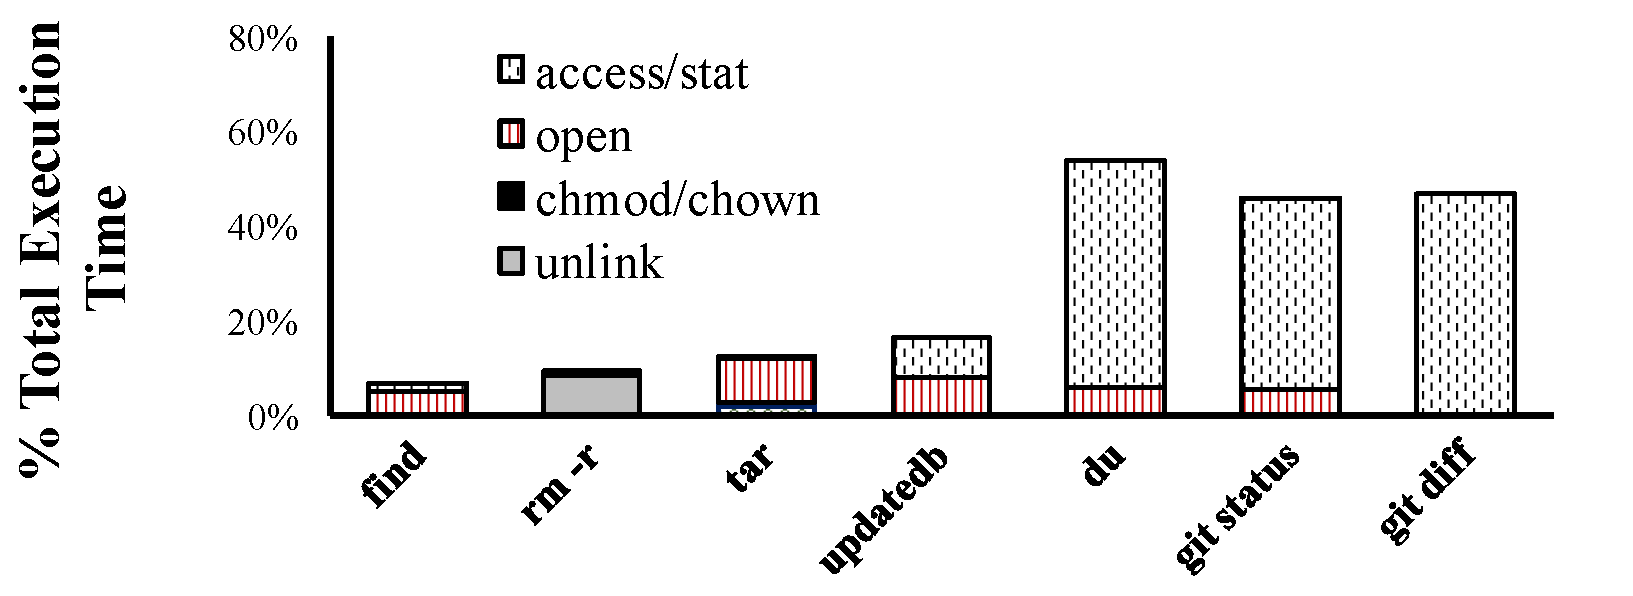
\includegraphics[width=5in]{dcache/plots/syscall-percentage.pdf} \\
\caption[Fraction of execution time on path-based system calls.]
{Fraction of execution time in several common utilities spent
executing path-based system calls with a warm cache, as measured with ftrace.}
\label{fig:dcache:lookup-frac}
%\vspace{-10pt}
\end{figure}

%\fixmedp{Please check these \% against time.  I think git diff is too high.  git status seems ok.}

Directory caches are essential for good application performance.
%Unix was designed such that ``(almost) everything is a file'',
%thus even accesses to in-memory file systems, device files, FIFOs and domain sockets
%first pass through the directory cache.
%In other words, 
Many common system calls must operate on file paths,
which require a directory cache lookup.
For instance, between 10--20\% of all system calls in the iBench system call traces do a path lookup~\citep{filenotafile}. 
Figure~\ref{fig:dcache:lookup-frac} lists the fraction of total execution time
%, as well as system time, 
several common command-line applications spend executing path-based system calls
(more details on these applications and the test machine in \S\ref{sec:dcache:eval}).
We note that these system calls include work other than path lookup,
and that these numbers include some instrumentation overhead;
% are coarse measurements that include  and work than path lookup;
%, and includes some time 
%for synchronous I/O (e.g., during {\tt rename}) as well as non-path tasks (e.g., creating 
%a file handle as part of {\tt open});
nonetheless, in all cases except {\tt rm},
the system call times and counts are dominated by
{\tt stat} and {\tt open}, for which 
%can be serviced from cache and for which 
path lookup is a significant component of execution time.
For these applications, path-based system calls account for 6--54\% of total execution time.
%and 25--77\% of system time.  
This implies that
lowering path lookup latency is
 one of the  biggest 
opportunities for a kernel to improve these applications' execution time.




\begin{figure}[t!]
\centering
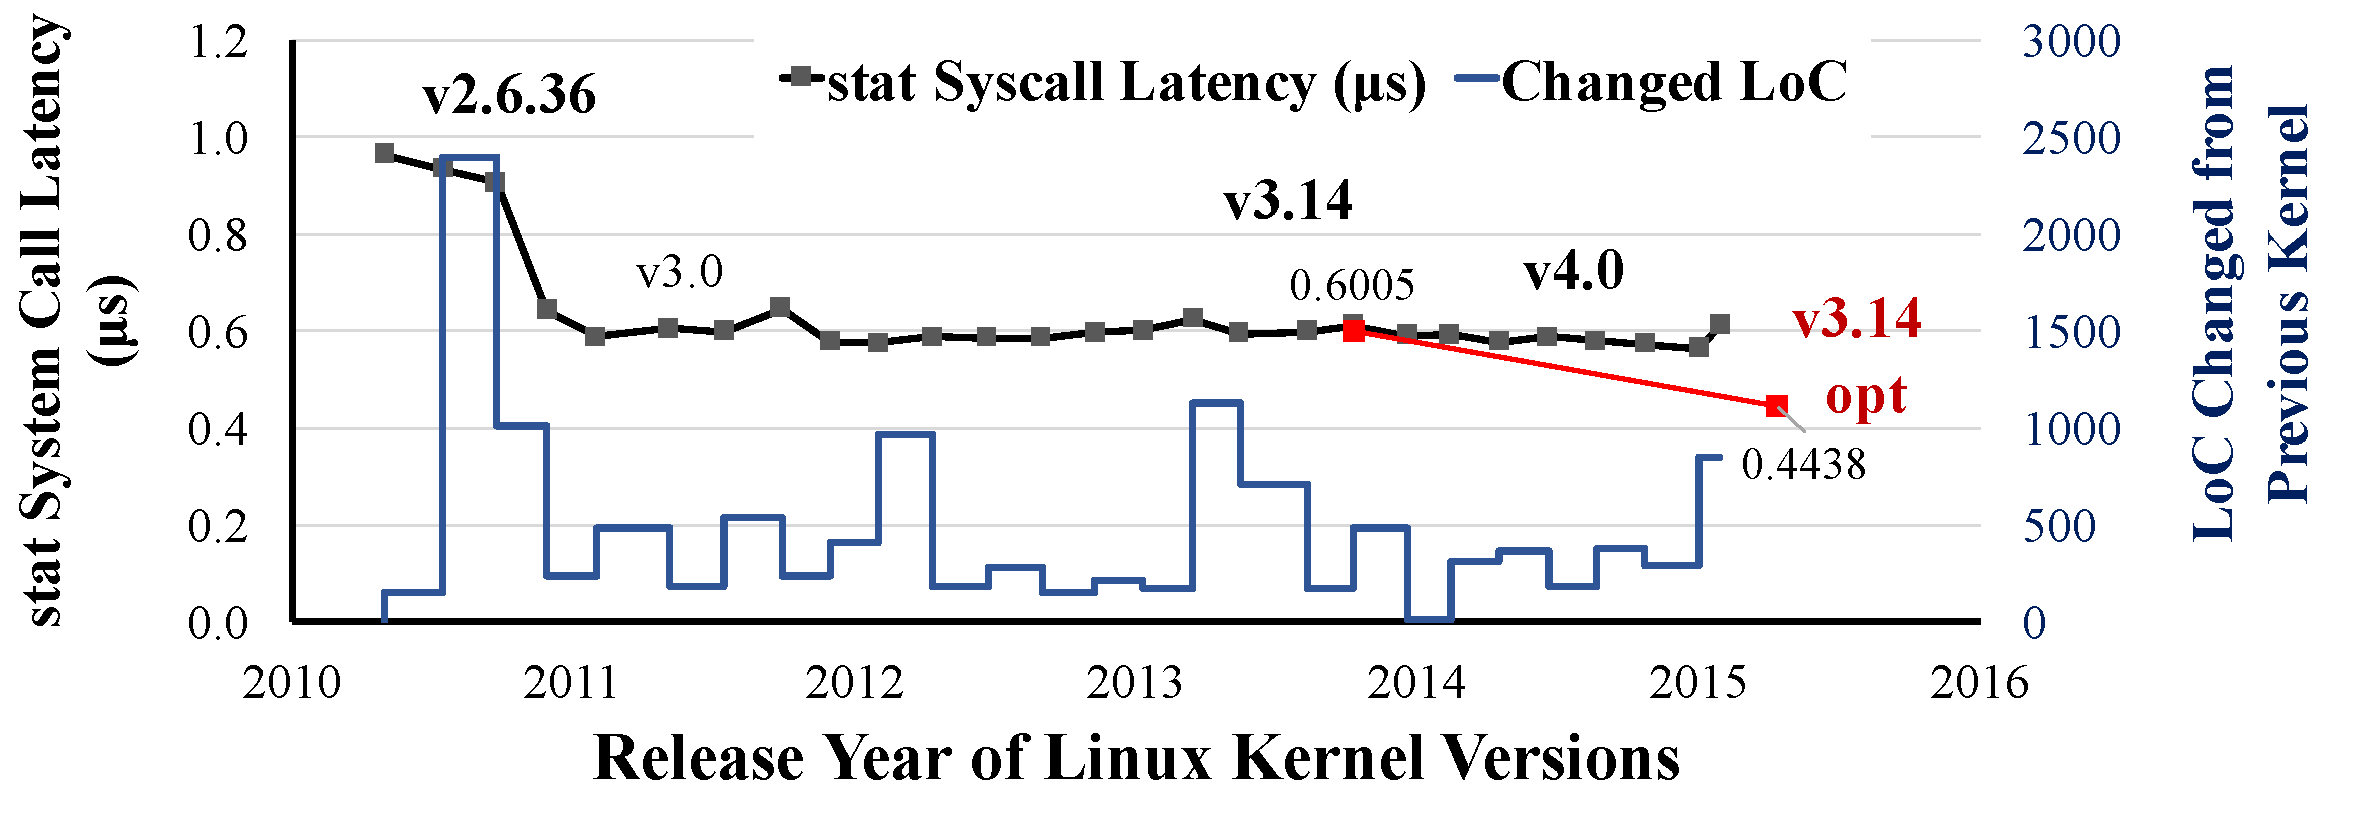
\includegraphics[width=6in]{dcache/plots/latency-by-version.pdf}
\footnotesize
\caption[Lantecy of {\tt stat} system call over years.]
{Latency of {\tt stat} system call with a long path {\tt XXX/YYY/ZZZ/AAA/BBB/CCC/DDD/FFF} on Linux over four years (lower is better), as well as the churn within the directory cache code (all insertions in {\tt dcache.c}, {\tt dcache.h}, {\tt namei.c}, {\tt namei.h} and {\tt namespace.c}). 
%Our optimizations significantly improve performance that has otherwise plateaued, despite significant ongoing developer effort.  
Our optimized \linuxver{} kernel 
further reduces {\tt stat} system call latency by \statspeedup{}\%.}
%\vspace{-15pt}
\label{fig:dcache:by-version}
\end{figure}


%\fixmedp{Add more evidence of lookup importance here: For instance, fraction of lookup time in file-related syscalls, or total lookup time in applications bound on file lookup latency.  }
Unfortunately, even directory cache hits are costly---0.3--1.1 \us{} for a {\tt stat} on our test Linux system, compared to only .04 $\mu$s for a {\tt getppid} and 0.3 \us{} for a 4 KB {\tt pread}. 
%\fixmetsai{Don, check this, I think read will be a better example, getppid is too trivial.}
This issue is taken particularly seriously in the Linux kernel community, which has 
made substantial revisions and increasingly elaborate optimizations to reduce the hit cost
of its directory cache, such as removing locks from the read path or replacing lock ordering with deadlock avoidance in a retry loop~\citep{corbet09jls,dcache-rcu}.
Figure~\ref{fig:dcache:by-version} plots directory cache hit latency against  lines of directory cache code changed 
over several versions of Linux, using a path-to-inode lookup \microbench{} on the test system described
in \S~\ref{sec:dcache:eval}.
These efforts have improved hit latency by 47\% from 2011 to 2013, but have plateaued
for the last three years.
%\fixmedp{if time, filter irrelevant changes from code deltas}
%at the cost of substantial developer effort.
%This latency appears to have plateaued 

The root of the problem is that the POSIX path permission semantics
seemingly require work that is linear in the number of path components,
and severely limit the kernel developer's implementation options.
%The root of this problem is that current directory cache
%designs reflect a straightforward implementation of the POSIX specification,
%which would seemingly require work that is linear in the number of path components.
For instance, in order to open file {\tt /\fnone{}/\fntwo{}/\fnthree{}} 
%for reading, 
one must have search permission
to parent directories {\tt /}, {\tt /\fnone{}}, and {\tt /\fnone{}/\fntwo{}},
as well as permission to access file {\tt \fnthree{}}.
The Linux implementation %of this specification is straightforward, 
simply walks the directory
tree top-down to check permissions.  
Unfortunately, when the critical path is dominated by 
walking a pointer-based data structure, 
including memory barriers on some architectures for multi-core consistency, 
modern CPUs end up stalling on hard-to-prefetch loads.
Moreover, because so many Linux features are built around this behavior, such as Linux Security Modules (LSMs)~\citep{wright+lsm},
namespaces, and mount aliases, it is not clear that any data-structural enhancements
are possible without breaking backward-compatibility with other Linux kernel features.
A priori, it is not obvious that a faster lookup algorithm, such as a single hash table lookup, 
can meet these API specifications and kernel-internal requirements; to our knowledge,
no one has tried previously.

%This paper proposes a decomposition of the directory cache, which allows
%most lookup operations to execute with a single hash table lookup (\S\ref{sec:dcache:dcache}),
%as well as optimizations to reduce the miss rate based on information that is {\em already in the cache}, but not used effectively (\S\ref{sec:dcache:readdir}).
%Our design maintains compatibility (\S\ref{sec:dcache:generalize}) through 
%several essential insights, including 
%how to separate the indexing of paths from checking parent permissions,
%and how to effectively and safely memoize the results of access control checks.


%% This paper proposes several new ways to organize a directory cache, which can yield 
%% substantial performance improvements over the current state of the art.
%% %This paper demonstrates that, despite this developer effort, there is still a substantial 
%% %missed opportunity hiding behind historical, intuitive, but not fundamental design choices.
%% Most of the Linux directory cache design reflects a straightforward implementation of the POSIX 
%% specification. %, with a division of labor that is suitable for mainstream file systems.

%This paper presents an alternative directory cache organization, which 
%improves performance by separating logical tasks, such as separating path indexing from permission checking; yet the design is sufficient to retain compatibility with POSIX.
%In the case of path lookup, 
%this paper demonstrates how 
%a per-component tree walk can be replaced with a single hash table lookup (\S\ref{sec:dcache:dcache}).
% without violating POSIX compliance.

%Our optimizations improve the performance of frequent lookup operations, but 
%introduce several costs, described in \S\ref{sec:dcache:dcache} and measured in \S\ref{sec:dcache:eval},
%which  we believe are acceptable and a net improvement for applications.
%First, these optimizations slow down infrequent modifications to the directory hierarchy, such as {\tt rename}, {\tt chmod},
% and {\tt chown} of a directory. 
%However, these slower operations
%account for less than .01\% of the system calls in the iBench traces~\citep{filenotafile}.
%Second,  the memory overheads of the dcache are increased.
%%(45\% per \dentry{}, as well as some  in our prototype).
%%(\fixmedp{XX MB} in our tests).  
%Third, lookup has a 
%probability of error from signature collisions that can be adjusted to be negligible
%%($2^{-141}$ in our configuration), 
%and within acceptable thresholds widely used by data deduplication systems~\citep{Debnath:2010:CSU:1855840.1855856, Srinivasan:2012:ILI:2208461.2208485, Quinlan:2002:VNA:645371.651321, Zhu:2008:ADB:1364813.1364831}.
%%, as well as how to remove
%%all memory barriers from the lookup path (\S\ref{sec:dcache:update}).
%In the micro-benchmark of Figure~\ref{fig:dcache:by-version}, our directory cache 
%optimizations improve lookup latency by 
%%revisions improve latency of accessing a long path
%%by 
%\statspeedup{}\% over unmodified Linux.
%%Our design addresses other missed
%%opportunities, such as identifying new opportunities to reduce the miss rate
%%through caching directory completeness.
%%\fixmedp{Do we want to highlight LoC?  3K is more than anything in the graph} \fixmetsai{Probably just mention in the evaluation. It's a metric that we should provide, but it's not awfully interesting.}
%%The total lines of code changed are fewer than 3,000 out of \fixmedp{XX}.
%%\fixmedp{Can we get 
%%, yet changes fewer than 3,000 lines of code.

%% SOSP cut - kind of long-winded
\begin{comment}
This paper rethinks current Linux directory cache design choices in light of the following goals:
\begin{compactitem}
\item {\bf Minimize the cost of a cache hit.} (\S\ref{sec:dcache:dcache}).
This means maximizing the benefit of temporal locality for frequent operations,
while pushing extra work of consistency maintenance onto less frequent, already-expensive operations.
%such as handling cache miss or updating massive metadata,
%in order to improve very frequent operations.
\item {\bf Maintain legacy compatibility.} (\S\ref{sec:dcache:generalize}).  Unix path semantics are complex, required by applications, file systems, and security modules, frustrating otherwise straightforward optimizations.  However tempting it may be to redesign path behavior to facilitate caching, path operations must exhibit the same behavior, with lower latency.
\item {\bf Never miss the same request twice in quick succession.} (\S\ref{sec:dcache:readdir}).  A number of less-frequent operations, such as reading a directory or secure temporary file creation, always miss in the cache {\em even if enough information is in cache to satisfy the operation.}  
%Of course, infrequent accesses should still be subject to a cache replacement policy, such as LRU.
\end{compactitem}
%Although directory caches must implement more complex semantics than a hardware memory cache,
%these principles should seem familiar to the reader with a basic architecture background.
%sadly, the Linux directory cache design violates all three.
\end{comment}

%This paper introduces several techniques to improve the performance of a directory cache,
%This paper explains several practical directory cache optimizations,
This paper demonstrates that these techniques improve performance for applications that use the directory cache heavily,
and the harm is minimal to applications that do not benefit.
%and that the worst case \microbench{} is only 12\% slower within \fixmedp{XX}\% of unmodified Linux.
%Each optimization we describe improves performance in isolation, and all can be combined.
%These optimizations change very few lines of code, and are backward-compatible with 
%legacy applications.  
%These changes are encapsulated in the VFS---individual file systems do not have to change their code.
%This paper describes a  prototype of these improvements implemented in Linux \linuxver{}.
%\S~\ref{sec:dcache:background} explains that the directory cache structure of Mac OS X, FreeBSD, and Solaris 
%are sufficiently similar that these principles should generalize.
%we compare and contrast Linux's directory cache
%with Mac OS X, FreeBSD, and Solaris in \S\ref{sec:dcache:background}, and explain inline how each
%optimization could be generalized to these other OS kernels.





%% \item {\bf Modularization and stackability}:
%% Any changes or optimizations must be implemented as modules inside Linux's VFS,
%% and can be stacked on top of the original design or any future optimizations. 
%% \item {\bf Backward compatibility}:
%% Any changes or optimizations must maintain least requirement of modifying any
%% file systems.
%% \item {\bf Generalization to other OSes}: Any changes or optimizations must be portable to other OSes with reasonable effort and change of design.




%% \dcache{} is proven to be effective on improving storage performance.
%% Experiments shows that,
%% in a Linux 3.x kernel, a \dcache{} with a xxx\% hit rate can speed up
%% metadata lookup and fetching time by xxx times.
%% \fixmetsai{experiment result, Linux version, and fs specs here}
%% However, we observed that Linux maintainers have made
%% constant and non-trivial efforts to improve \dcache{} in the Linux kernel.
%% We studied all \dcache{}-related source files in the Linux kernel Git repository,
%% and discovered that maintainers have committed
%% on average xxx revisions per source files.

%% We tested metadata lookup time on primary \dcache{}-related revisions.
%% Most changes on \dcache{} system only create xxx\%-xxx\% speed-up
%% than their predecessor.
%% \fixmetsai{result and graph here}.
%% Moreover, improvement to \dcache{} is still work-in-progress
%% for Linux maintainers.
%% \fixmetsai{reference to threads for latest dcache discussions}. 
%% All the evidences show that,
%% despite of significant reduction of storage operations,
%% efficiency of \dcache{} system internally still remains as a concern.

%% We argue that the design of \dcache{} needs to be carefully re-examined,
%% to fundamentally identify any missed opportunities that
%% improve value of \dcache{}.
%% At a high level, most optimization works for \dcache{} are focused on
%% improving ``how to cache'',
%% but we want to also lay eyes on ``what to cache'',
%% to ensure any valuable information returned from file systems
%% be captured by \dcache{} system.

%The contributions of this paper are as follows:
%\begin{compactitem}
%\item A performance analysis of the costs of path lookup and the opportunities
%to improve cache hit latency.
%\item A directory cache design that improves path lookup latency with a combination of techniques, including:
%  \begin{compactitem}
%  \item Indexing the directory cache by full path, reducing average-case lookup from linear to constant in the number of path components.
%  \item A Prefix Check Cache (PCC) that separates permission checking from path caching.  The PCC memoizes permission checks, and is compatible with LSMs~\citep{wright+lsm}.
%  \item Reducing the cost of checking for hash bucket collisions with path signatures.
%  \end{compactitem}
%\item Identifying opportunities to leverage metadata the kernel already has to reduce miss rates, such as tracking whether a directory is completely in cache.
%\item Carefully addressing numerous, subtle edge cases that would frustrate rote application of these techniques, such as integration with symbolic links and Linux namespaces.
%\item A thorough evaluation of these optimizations.  For instance, our optimizations improve throughput
%of the Dovecot IMAP server by up to \dovecotspeedup\% and latency of 
%updatedb by up to \updatedbspeedup{}\%.
%%git version control system by up to 25\%.
%
%\end{compactitem}

\chapter{System Overview}
\label{chap:graphene}

%\section{Introduction}
%\label{sec:graphene:intro}

Existing library OSes provide single-process applications
with the qualitative benefits of virtualization
at a lower cost~\cite{porter11drawbridge,unikernels,baumann13bascule}.
These benefits include security isolation of mutually untrusting applications,
migration, and host platform independence.
%Library OSes move portions of
%OS kernel functionality into an application library.
In a library OS, the guest OS is essentially ``collapsed''
into an application library,
%% dp: too early for this nomenclature, I think
% \daniela{(a libraryOS instance)},
which implements the OS system calls and abstractions required by legacy applications
and libraries.
The library maps high-level APIs onto a few narrowed interfaces
to the host kernel.
The reduction of host interfaces provides portability to various platforms that can translate the interfaces to host APIs or abstractions,
%and a narrower attack surface that developers can more likely reason about.
% and supporting data structures as library functions---mapping
%high-level APIs onto
%a few paravirtual interfaces to the host kernel.
%Recent library OSes improve efficiency over full guest OSes by eliminating duplicated features
%between the guest and host kernel,
%such as the CPU scheduler, or
%eliminating guest-level multiplexing code, as the library OS supports only one application;
%even compiling out unnecessary guest kernel APIs~\cite{unikernels}.
Compared with visualization, 
\liboses{} can eliminate duplicated features between the guest to the host kernel
such as the CPU scheduler or file system drivers.
Therefore, 
%In total, this can reduce 
the memory requirements of running a single, isolated application in \liboses{}
is  orders-of-magnitude
less than running it with visualization
~\cite{porter11drawbridge,unikernels}.
Library OSes have also been proven
useful for porting legacy applications
onto new hardware platforms, such as Intel's SGX enclaves~\cite{baumann14haven}.
%% dp: This sentence seems a little premature
%In recent works, library OSes provide rich OS features for isolated contexts while the host OSes are untrusted

%% Library OSes reduce the memory requirements of running a self-contained,
%% isolated application process
%% %guest \daniela{I would replaced guest by "isolated process or group of processes (a \libos{} instance)''}
%% by orders of magnitude
%% In a cloud computing environment,
%% increasing the number of applications per server has enormous
%% economic benefits.
%% Even on a desktop or portable system, \libos{}es can reduce the overheads
%% of sandboxing untrusted code and running applications
%% designed for another OS.

%Because library OSes execute within a VM \daniela{this phrase does not read good to me because (i) it might imply the picoprocesses need hypervisor support, as misunderstood by reviewer 1 and (ii) you already emphasized the drawbacks of leveraging a VM} or lightweight process ({\em picoprocess}~\cite{xax}),
%library OSes execute with

%% dp: Daniela, great suggestion!  We need to make this situation seem more
%%     like the sky will fall without our help
A key drawback for recent \liboses{} to run legacy applications, however,
is that the support in these \liboses{} are mostly limited to single-process applications.
Many applications, such as network servers and
shell scripts,
create multiple processes
for
performance scalability, fault isolation, and programmer convenience.
%These applications would benefit from the efficiency and security benefits
%of a library OS.
In order for the efficiency benefits of library OSes to be widely applicable,
especially for unmodified Unix applications,
%either applications must be rewritten to implement ad hoc coordination mechanisms, or
library OSes must provide commonly-used multi-process abstractions,
such as fork,  signals, \sysvipc{} message queues and semaphores, sharing file descriptors, and exit notification.
Without sharing memory across \picoprocs{},
\libos{} must coordinate shared OS states to support multi-process abstractions.
%To support multi-process abstractions, library OSes often have to rely on sharing OS states,
%backed by the hosts' memory sharing features.
For example, Drawbridge~\cite{porter11drawbridge} cannot simulate process forking because copy-on-write memory sharing is not a platform-independent features.


\begin{figure}[t!]
\centering
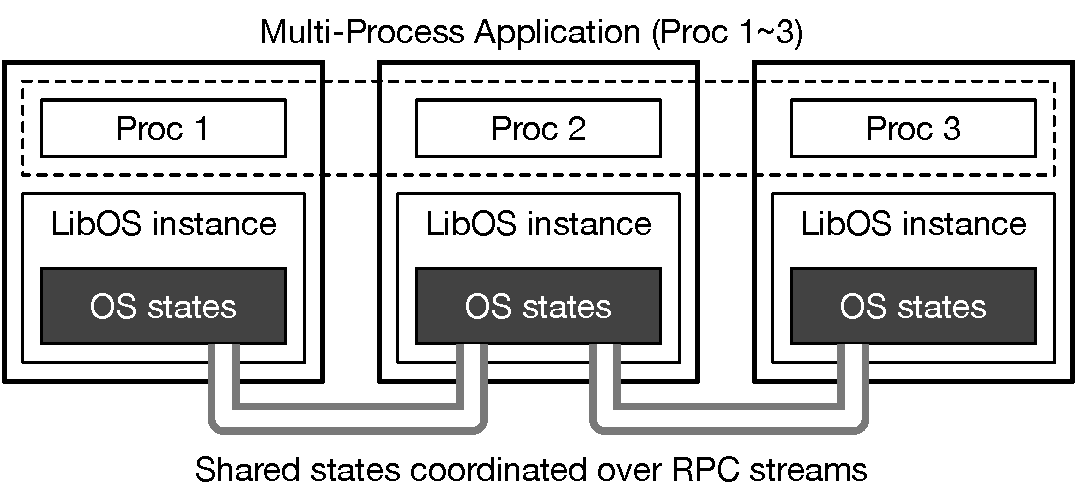
\includegraphics[width=4in]{graphene/figures/concept.pdf}
\caption[Multi-process support model of \graphene{} \libos{}]
{Multi-process support model of \graphene{} \libos{}. For each process of an application, a \libos{} instance will serve system calls and keep local OS states. States of multi-process abstractions are shared by coordinating over host-provided RPC streams, creating an illusion of running in single OS for the application.}
%\vspace{-.1in}
\label{fig:graphene:concept}
\end{figure}

{\bf \graphene{}} is a Linux-compatible library OS
to run legacy, unmodified Linux applications.
In \graphene{}, multiple \libos{} instances collaboratively implement
POSIX abstractions,
yet appear to the application
as a single, shared OS.
\graphene{} instances coordinate state using remote procedure calls (RPCs) over
host-provided byte streams (similar to pipes).
In a distributed POSIX implementation, placement of shared state and messaging complexity
are first-order performance concerns.
%We chose to shift implementation complexity into the library OS
%in order to uphold simple enforcement of security isolation in the host.
By coordinating shared states across \libos{} instances,
\graphene{} is able to create an illusion 
of running in a single OS
for multiple processes in an application (as figure~\ref{fig:graphene:concept}).
%Previous library OS designs ensured security isolation of independent applications,
%comparable to a VM, by keeping a relatively narrow host ABI.
%We selected the \graphene{}
%design because it strikes a unique balance between
%and robust, flexible security enforcement.
The \graphene{} design ensures security isolation of
mutually distrusting, multi-process
applications on the same host system.
Essential to this goal is
minimally expanding the host ABI to support multi-processing,
as well as leveraging RPCs as a natural point to mediate inter-\picoproc{} communication.
RPC coordination among \graphene{} instances can be dynamically disconnected, facilitating novel sandboxing
techniques.  For instance, we develop an Apache web server extension that, upon logging in a given user,
places the worker process's \libos{} in a sandbox with access to only that user's data.
We expect more nuanced degrees of trust are possible in future work.

\begin{comment}
The contributions of this paper are:
\begin{compactitem}
\item \graphene{}, a Linux library OS, which supports
  real-world, multi-process applications including a shell, web server,
  and compiler, which can be  efficiently checkpointed and migrated.
% \fixmetsai{We need to enable mulit-process checkpointing and migration}
% \daniela{the reviewers will be looking for that in the experiments section: "among hosts''}.
\item A framework for implementing multi-process APIs across cooperating library OS instances.
%\daniela{I would change to: "A thorough security analysis of \graphene{} isolation design'' You mention that you trust the reference momitor, so there is no security to
%be evaluated unless you guarantee the process is not vulnerable to exploits. We have not evaluated the security of the coordination design, only the isolation. To evaluate the security to the coordination design we have to look at possible race conditions and how they are dealt with.}
%\item Addressing additional challenges developing a robust Linux library OS, including copy-on-write fork.
\item A thorough evaluation of the overheads of \graphene{}.  Memory footprints are an order of magnitude
smaller than KVM, and several applications perform comparably to a Linux process.
\item A thorough analysis of \graphene{} security isolation.

%In the best case, the overhead of a large {\tt gcc} compilation on \graphene{} is only 3\%.

\end{compactitem}
\end{comment}

%\graphene{}'s design gives the user and system administrator a high degree of flexibility
%in isolating arbitrary groups of unmodified application processes,
%while upholding the efficiency and host compatibility benefits of recent library OSes.

%\fixmedp{After a complete draft is written, coalesce all goals and make sure they are addressed early on.  We are doing some scatter-shot motivation}


\section{Implementing Linux Personality}
\label{sec:graphene:background}

%Recent library OSes~\cite{porter11drawbridge,unikernels,baumann13bascule,osv}
%are designed for security and efficiency, but are limited to single-process applications.
%The security isolation of \liboses{} derives from 
%limited, explicit data sharing and 
%a narrow host interface.  
A \libos{} typically executes in either a paravirtual VM~\cite{unikernels,osv}
% \daniela{I would have the use of a VM as a discussion topic in the end of the paper.}, 
or an OS process, called a \emph{\picoproc{}}~\cite{porter11drawbridge,baumann13bascule},
with an interface restricted to a narrowed set of host kernel ABIs.
These host ABIs heavily restrict effects outside of the application's address space;
as a result, applications in a \picoproc{} have very little opportunity to interfere with each other,
yielding security isolation comparable to a VM.
Library OS efficiency comes from deduplicating features, such as hardware management;
in a VM these features typically appear in both the guest and host kernels.


\graphene{} executes within a \picoproc{} (Figure~\ref{fig:graphene:arch}),
which includes an \emph{unmodified} application binary and supporting libraries, 
running on a \libos{} instance.
The \libos{} is implemented over a host kernel ABI
designed to expose very generic abstractions that can be easily 
implemented on any host OS, including virtual memory, threads, synchronization, byte streams (similar to pipes),
a file system, and networking.
Although the \graphene{} prototype  host kernel is Linux, 
we adapt a host ABI from Drawbridge/Bascule,
which has been previously implemented on Windows, Hyper-V, and Barrelfish~\cite{porter11drawbridge,baumann13bascule,baumann09barrelfish}.
%The \graphene{} host ABI is
% summarized in Table~\ref{tab:abi} and discussed in more detail in \S\ref{sec:linux:pal}\fixmedp{if not cut...}.  
%which exposes only tens of simple host calls. \daniela{briefly define \picoproc{}: A \picoproc{} is unmodified application code running with a \libos{}.}


\begin{figure}[t]
\centering
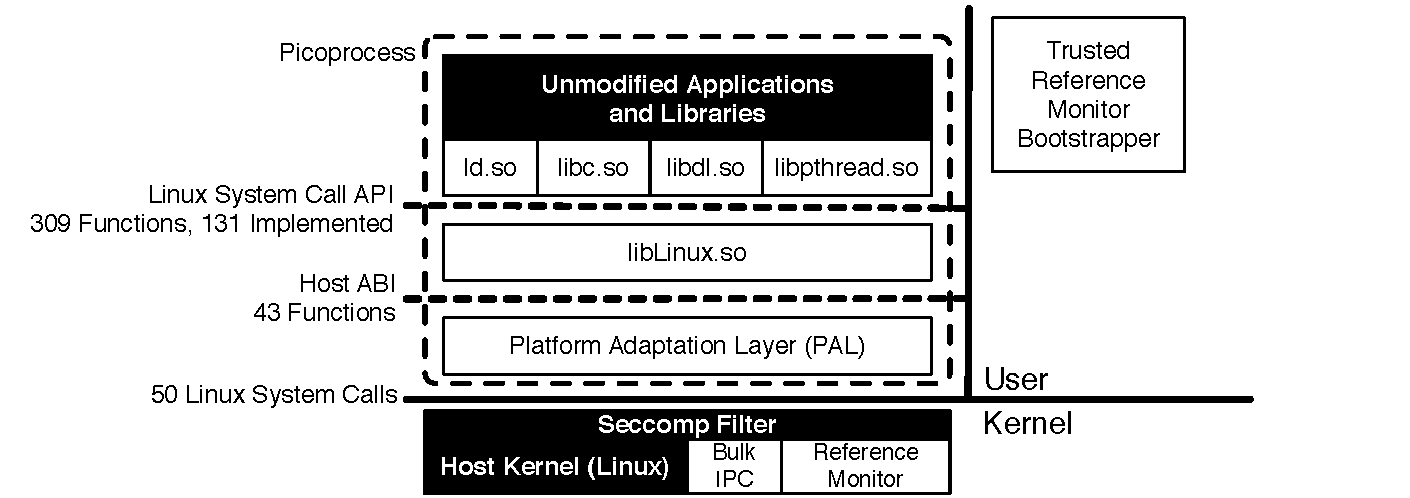
\includegraphics[width=6.5in]{graphene/figures/arch.pdf}
\caption{Building blocks of \graphene{}.  Black components are unmodified.
We modify the four lowest application libraries on Linux:
{\tt ld.so} (the ELF linker and loader),
{\tt libdl.so} (the dynamic library linker),
{\tt libc.so} (standard library C),
and {\tt libpthread.so} (standard threading library),
that issue Linux system calls as function calls directly to {\tt libLinux.so}.
Graphene implements the Linux system calls
using a variant of the Drawbridge ABI,
which is provided by the Platform Adaptation Layer (\pal{}),
implemented using calls to the kernel.
A trusted reference monitor that ensures \libos{} isolation
is implemented as a kernel module.
Another small module is added for fast bulk IPC.}
\label{fig:graphene:arch}
\end{figure}


\graphene{} exports \palcalls{} host ABIs through a 
Platform Adaptation Layer (\pal{}) (Table~\ref{tab:graphene:abi}).
The \pal{} is a binary injected into the \picoproc{} by the host, 
and translates the generic \picoproc{} ABI into host system APIs.
Most of these calls only affect the application-internal state;
any calls with external effects are mediated by a trusted \emph{reference monitor} on the host.
%The reference monitor is a trusted non-\graphene{} process running on the system.
All \graphene{} applications are launched by the reference monitor,
which installs a system call filter and interposes on permitted kernel calls to ensure isolation
(\S\ref{sec:graphene:security}).


These \pal{} ABIs should be a sufficient substrate upon which to
implement guest-specific semantics, or guest \emph{OS personality}.
As an example of this layering, consider the heap memory management abstraction.
Linux provides applications with a data segment---a 
legacy abstraction dating back to original Unix and the era 
of segmented memory management hardware.
The primary thread's stack is at one end of the data segment, and the heap is at another.  
The heap grows up (extended by {\tt sys\_brk}) 
and the stack grows down until they meet in the middle.
In contrast, the \pal{} ABI provides only three simple functions 
that allocate, protect, or unmap regions of virtual memory
with basic access permissions (read, write, and execute).
This clean division of labor encapsulates 
idiosyncratic abstractions in the library OS,
and eliminates the need for
redundant hardware management code, 
such as duplicate low-level page management and swapping heuristics.


%These interfaces are host-independent \daniela{OS or kernel-independent}, as they tend to be very generic and easily
%implemented on any host OS kernel or VMM \daniela{postpone VMM for later}.

At a high level, these library OS designs
scoop the layer just below the system call table out of the OS kernel
and refactor this code as an application library.  
The driving insight is that there is a natural, functionally-narrow division point 
one layer below the system call table
in most OS kernels.
Unlike many OS interfaces, these \pal{} ABIs generally minimize the amount of application state in the kernel, facilitating
migration: a \picoproc{} can programmatically read and modify its own OS state,
copy the state to another \picoproc{}, and the remote \picoproc{} can 
load a copy of this state into the OS---analogous to hardware registers.
A \picoproc{} may not modify another \picoproc{}'s OS state.



%% To implement the Linux OS
%% personality, we introduce 1 ABI for managing x86 segment registers and
%% 2 for handling runtime hardware exceptions.  The extensions are
%% expected to uphold host compatibility since they are also identified
%% and introduced in Bascule. In addition, 6 new ABIs, including
%% copy-on-write page exchanges, stream handle sharing, and sandbox
%% creation, are introduced to improve either efficiency or security
%% isolation of library OSes. These ABIs can always fall back to the
%% Drawbridge/Bascule ABIs if users decide to prioritize compatibility.

\begin{comment}
\begin{table}[t]
\footnotesize
\centering
\begin{tabular}{|l|c|>{\palign{l}}p{4.8in}|}
\hline
\multicolumn{3}{|c|}{\bf Adopted from Drawbridge} \\
\hline
{\bf Class} & {\bf ABIs} & {\bf Description} \\
\hline
Memory & 3 & Allocate and protect virtual memory. \\
\hline
Scheduling & 12 & Threads and synchronization. \\
\hline
Files \&  Streams & 12 & Files inside a {\tt chroot}-style; jails and byte streams among \picoprocs{}. \\
\hline
Process & 2 & Create a child \picoproc{}, and exit self. \\
\hline
Misc & 4 & Get random bits, time of day, etc. \\ % flush instruction cache, etc.\\
\hline
\multicolumn{3}{|c|}{\bf Added by \graphene{}} \\
\hline
{\bf Class} & {\bf ABIs} & {\bf Description} \\
\hline
Segments & 1 & Manage x86 segment registers (FS and GS) for TLS. \\
\hline
Exceptions & 2 & Handle hardware exceptions. \\
\hline
Streams & 4 & Share stream handles across \picoprocs{}, rename files, and set stream attributes (file permissions, socket options, etc.) \\
\hline
Bulk IPC & 3 & Exchange copy-on-write pages.\\
\hline
Sandboxes & 1 & Move into a new sandbox, with a new manifest applied. Pipes and streams that violates the new policy are closed.\\
\hline
\end{tabular}
\caption[List of host ABI functions defined in \graphene{}]
{Classes of  host ABI functions adopted from \drawbridge{}~\cite{porter11drawbridge}, 
followed by ABIs added by \graphene{}.}
\label{tab:graphene:abi}
\end{table}
\end{comment}

\fixme{Need transition to next section.}

\subsection{Multi-Process Support in Library OSes}

A key design feature of Unix is that users compose simple utilities to create
larger applications.  Thus, it is unsurprising that many popular applications for Unix or Linux
require multiple processes
--- an essential feature missing from current \libos{} designs.
%This gap is filled by the \graphene{} \libos{}, which
%extends recent \liboses{} to support multi-process applications.
The underlying design challenge is minimally expanding 
a tightly-drawn isolation boundary
without also exposing idiosyncratic kernel abstractions or
re-duplicating mechanisms \fixme{Discuss deduplicating features upfront} in both the kernel and the \libos{}.

%requires a careful balance among the competing goals of 
%efficiency, host independence, and security isolation.
%The challenge, then, is minimal expansion of

%\vspace{5pt}
%\noindent {\bf Motivating Example.~}
For example,
consider the process identifier (PID) namespace.
In current, single-process lib\-OSes, 
the {\tt getpid()} system call could simply return a fixed value to each application.
This  single-process design is isolated,
but the library OS cannot run a shell script, which requires {\tt fork}-ing and {\tt exec}-ing multiple binaries, signaling, waiting, and other
PID-based APIs.

\vspace{5pt}
\noindent{\bf Design Options.~}
Multi-process  support requires extensions to the \pal{} ABI of recent, single-process \libos{} designs.
Because multi-process abstractions, 
such as signals or System V IPC, 
tend to be idiosyncratic,
an essential problem is identifying a minimal, host-independent
substrate upon which 
to implement OS-specific abstractions.

We see two primary design options:
(1) implement processes and scheduling in 
the library OS, and (2) treat each \libos{} instance as a process, and distribute the 
shared POSIX implementation across a collection of \liboses{}.
We selected the second option, primarily because we expected this would impose fewer
requirements on the host, maximize flexibility in mapping processes 
to physical resources, and facilitate inter-process security policy enforcement. % as enforcing security policies on related processes.

Implementing processes
inside the library OS is also feasible using 
hardware MMU virtualization, similar to Dune~\cite{belay12dune},
but this reintroduces a duplicate scheduler and memory management.
Moreover, Intel and AMD have similar, but mutually incompatible MMU virtualization support,
which would complicate live migration across platforms.
None of these problems are insurmountable, and it would be interesting in future
work to compare both options.

\paragraph{Multi-Process Support in \graphene{}.}
%\daniela{Because Approach and Motivating Example are on the same level, its seems that
%you are starting a new topic under Approach, when the discussion is actually a continuation of
%Motivating Example}
In \graphene{}, multiple \libos{} instances in multiple \picoprocs{} collaborate to 
implement shared abstractions, such as 
 copy-on-write fork, signals, exit notification,
and System V IPC.
For instance, when process A signals process B on \graphene{}, A's \libos{} issues
a remote procedure call (RPC) to B's \libos{} over a host-provided byte stream (similar to a Unix pipe),
and B's \libos{} then calls the appropriate signal handler.

%%% All collaborating \libos{} instances exchange messages as needed 
%%% to provide the application with a consistent view of 
%%% shared abstractions,
%%% such as


%\graphene{} approaches multi-processing by selectively replicating state and issuing remote procedure calls (RPCs) 
%%across multiple, collaborating
%library OS instances.
%Guests may work together to provide the unmodified multi-process application with
%coordination abstractions 

%Shared abstractions on \graphene{}'s are implemented outside of the host, ensuring  host OS independence.
% by implementing these
%shared abstractions entirely
%outside of the host kernel.
%Shared abstractions are implemented outside of the host.
%From the host kernel's perspective, 
\graphene{} implements all shared abstractions in the \libos{}, and \liboses{} cooperatively manage these abstractions
over RPC streams.
Single-process applications still service system calls from local state, and \graphene{} 
includes optimizations to place state where it is most likely to be used,
minimizing RPC overheads.
The host reference monitor can easily isolate \liboses{}
by 
% \graphene{} design isolates \liboses{} by 
%requiring all coordination to use 
%explicit bytes streams \daniela{, pipe-like abstractions provided by the kernel. (suggestion: Reviewer  3)}.
%Security isolation is enforced
%by a kernel-level {\em reference monitor}, which can 
%disconnect or prevent creation of a
blocking all
RPC messages, % between \liboses{} that should be isolated,
without the need to understand the \libos{} details or semantics of these abstractions.
In our PID example, only mutually-trusting \liboses{} can signal each other.
%if the reference monitor prevents creation of RPC streams
%across mutually untrusting \picoprocs{},
%the \liboses{} cannot exchange signals.

%%% \graphene{} is designed to 
%%% The \graphene{} design leverages a number of optimizations to service application system calls 
%%% from local state whenever possible, and to minimize message passing overheads otherwise
%%%  (\S\ref{sec:namespaces:insights}).
%%% Our experience is that starting with a local system call design and then extending it to share state is relatively straightforward,
%%% and introduces little-to-no overhead when the request can be serviced locally.


The \graphene{} library OS is designed
to gracefully handle disconnection from other \liboses{}, 
facilitating dynamic application sandboxing.
RPC streams may be disconnected at any time by 
either the reference monitor or at the request of a \libos{}.
%Message streams may be severed externally, by the reference monitor, or 
%one guest may simply disconnect from others to isolate itself.
%An application may disconnect itself from the 
%Any \graphene{} application may dynamically detach from the confederation, 
%or a host-level sandbox may dynamically separate two guests by severing their communication channels.
When \graphene{} \liboses{} are disconnected, each instance will handle the subsequent
divergence 
%and the library OS will will fork these abstractions
{\em transparently} to the application.
For instance, if a child process is disconnected from the parent by the reference monitor,
each \libos{} will interpret the event as if the other process terminated---closing any open pipes,
delivering exit notifications, etc.
% \daniela{(applications run unmodified) - Reviewer 1 asked clarification on transparently}.

%% A key insight behind our design is that the common use case for these \daniela{cooperating} abstractions
%% is between a pair of processes.  Thus \graphene{} leverages a number of optimizations 
%% to reduce broadcast messages, avoid replication of needless state,
%% and service requests locally


\paragraph{Changes to \pal{} ABI.}
When implementing \graphene{},
we found that the Drawbridge ABI lacked 12 \pal{} calls
essential to running a Linux \libos{} with multi-process support, and 
\graphene{} did not require 3 \pal{} calls to support checkpoint and resume.
Of the 12 new calls, 4 are required for single-process Linux and similar ABI have also been added by \emph{Bascule}~\cite{baumann13bascule}:
rename a file, manage segmentation hardware, and 2 for exception upcalls;
5 are required for stream inheritance, attribute configuration, and sandboxing;
and 3 new calls are used to utilize Bulk IPC channel, for optimizing copy-on-write fork (\S\ref{sec:graphene:impl}).
%Our design requires only 11 additional \pal{} calls, which we believe are fundamental to executing 
%Unix-style multi-process applications.
We design these new \pal{} calls in consideration of the platform independence
among different hosts;
If a \pal{} call is added for optimizations (e.g., Bulk IPC),
it is optional if the implementation is difficult or infeasible on a host.
%in case that the new \pal{} calls are not possible to implement on a host,
%the 
%Our design deliberately provides options where these new \pal{} calls are missing, to preserve the platform importance proven by \emph{Drawbridge}~\cite{porter11drawbridge}.
For example, copy-on-write forking can still be supported
without Bulk IPC supported on the host.
Instead, the inheritance of process state for
copy-on-write forking will be completely over regular pipes.

\paragraph{Comparison with \microkernel{}s.}
The building blocks of \graphene{} are very similar to the system abstractions of a 
\microkernel{}~\cite{liedtke95sosp,klein09sel4,elphinstone13microkernels,liedtke93sosp,chen93memory,Baron:1985:MOE,Accetta:1986:MNK},
except a \microkernel{} often has a even narrower, more restricted interface
than the \pal{} ABI.
%such as the port and
%message abstractions of Mach~\cite{
Unlike a multi-server \microkernel{} system, such as GNU Hurd~\cite{hurd} or Mach-US~\cite{stevenson95mach-us},
which implements Unix abstractions across a set of daemons that are shared by all processes in the system,
\graphene{} implements system abstractions as a library in the application's address space,
and can coordinate library state among \picoprocs{} to implement shared abstractions.
\graphene{} guarantees isolation equivalent to running 
an application on a dedicated VM; this isolation could be implemented on a multi-server \microkernel{}
by running a dedicated set of service daemons for each application.

%%% \graphene{}'s differences are motivated by two considerations: efficient support of both stand-alone, 
%%% single-process applications and multi-process applications; as well as flexible security isolation. 
%%% \graphene{} contributes techniques to seamlessly and efficiently transition 
%%% between single-process and multi-process support, as well as adapting 
%%% some known techniques to a new environment.

The \graphene{} host ABI could be described as a hybrid \microkernel{},
which also exposes the file system and network of the host kernel.
Similarly, we assume that \picoprocs{} are provided by a legacy OS kernel, like Linux or Windows,
or by a Type 2 hypervisor.  We expect that a bare metal hypervisor could export a \pal{},
but would probably require services from a trusted VM, such as Xen's dom0~\cite{barham03xen}.
%or the \pal{} would implement more thread scheduling, networking, and file system code;
%or the \pal{} ABI would change to push this code into the \libos{}.
Arguably, recent \libos{} designs might be improved by rethinking the division of labor in
the network and file system stacks, but this is beyond the scope of this thesis.

\paragraph{Alternatives.}
Another approach to support multi-process applications in a \libos{} 
would be to use hardware MMU virtualization such as nested paging
used by a system like Dune~\cite{belay12dune}
in order to implement a second process abstraction, memory manager, and scheduler in the \libos{}.
This approach threatens the efficiency benefits of deduplicating these features.
A final option is exposing additional kernel interfaces, such as signals, 
by adding more system calls to a \picoproc{}.
This approach undermines host independence, as many of these coordination abstractions 
tend to be very OS-specific.
%Unix signals vs.\ Windows events, {\tt waitpid()} vs.\ blocking on a process handle, etc.
This approach also harms security isolation, as the \libos{} now has access to generally 
porous host kernel interfaces.  
%Although legacy OSes do enforce some access control rules on coordination abstractions,
%kernel developers must audit and add hooks to millions of lines of code.
%As a result,
%users have lost confidence that a traditional OS can comprehensively enforce 
%security isolation on these abstractions---a key motivation for using VMs
%for security isolation.


Systems must strike a careful balance between the competing goals of
security isolation and
multi-process coordination.
Multi-process applications require OS-managed coordination abstractions
such as signals, process exit notification, and System V IPC.
These coordination abstractions operate within shared namespaces, such as the 
process ID namespace
and the System V key space.
These coordination APIs and namespaces must be consistent among coordinating processes,
but can %introduce information leaks and 
undermine security isolation among unrelated processes on the same host.
System designs generally only meet one goal: 
traditional OSes have a rich but porous coordination interface, 
while sandboxing systems and virtual machines (VMs) 
are strictly isolated.
This thesis demonstrates that this unfortunate trade-off is not
fundamental.
%coordination or isolation.  


Traditional OS kernels typically provide  rich multi-process coordination 
APIs, but this richness also makes for a very porous attack surface
area.  For instance, on Windows, a program may inject libraries and
create threads in another program~\cite{windows-dll-inject}; 
similarly, unchecked file descriptor inheritance in Linux can lead to
security problems~\cite{close-on-exec}.  
Although legacy OSes do enforce some access control rules on these abstractions,
kernel developers must audit and add hooks to so much code
that
users have lost confidence that an OS can comprehensively enforce 
security isolation on these abstractions.

For achieving strong security isolation on applications,
%generally lost confidence that legacy OSes can robustly enforce security isolation, and 
users have turned to virtual machines (VMs).
For instance, if two customers host their websites in the same cloud service,
the customers will insist on running their web servers in separate VMs for security.
VMs take a heavy-handed approach to security isolation --- ensuring 
that every application has a dedicated OS kernel in a hardware-isolated address space.
Although virtual machines isolate
applications and provide legacy OS abstractions within a VM, 
coordinating applications must be statically placed in the same VM,
and cannot dynamically move to a separate VM.
For instance, consider a web service running
inside of a VM that wishes to isolate requests for different users in
different VMs after authentication.  The web server administrator must
statically create a VM for each user, introducing substantial
overhead; and the developer loses convenient IPC abstractions and
must rewrite large swaths of code.

\section{Coordinating Guest OS States}
\label{sec:graphene:namespaces}

%\fixmedp{RF: what are the few, powerful mechanisms?  Expect that there are many cases 
%with shared state; re-read this to see if it is clear how to generalize the approach}

%Recent library OS designs focus on single-process applications,
%which move a substantial portion of the OS APIs and state used by the application into the \libos{}.

%A key contribution of the \graphene{} 
%design is robust and flexible support for multi-process applications.
An application executes on \graphene{} 
with the abstraction that all of its processes are running on a single OS.
\graphene{} \libos{}es service system calls
from local \libos{} state whenever possible,
and state is coordinated across \picoprocs{} via RPC when necessary.
Within a sandbox, \graphene{} \picoprocs{} 
coordinate shared state used to implement multi-process
abstractions, such as process identifiers, thread groups, and 
System V IPC including message queues and semaphores, shared file system and file descriptor states (Table~\ref{tab:graphene:multiproc}).
Similar to previous designs~\cite{porter11drawbridge,baumann13bascule}, 
\graphene{} uses the host file system; 
the \libos{} implements file handles and translates between POSIX and the host ABI.
Identifying the best division of labor for a \libos{} file system is 
left for future work.

\begin{comment}
\begin{table}
\footnotesize
\centering
\begin{tabular}{|p{0.9in}|p{1.5in}|p{3.6in}|}
\hline
{\bf Ab\-strac\-tion} & {\bf Shared State} & {\bf Strategy} \\
\hline
Fork & 
\raggedright
PID namespace & Batch allocations of PIDs, children generally created using local state at parent.  \\
\hline
Signaling & PID to \picoproc{} map & Local signals call handler; remote signal delivery by RPC.  Cache mapping of PID to \picoproc{} ID. \\
\hline
\raggedright
Exit notification & 
\raggedright
Remote process status  & Exiting processes issue an RPC, or one synthesized if child becomes unavailable.  The {\tt wait} system call blocks until notification received by IPC helper. \\
\hline
{\tt /proc/[pid]} & Process metadata & Read over RPC.  \\
\hline
Message Queues & 
\raggedright
Key mapping, queue contents & Mappings managed by a leader, contents stored in various \picoprocs{}.  When possible, send messages asynchronously, and migrate queues to the consumer.\\
\hline
Semaphores & 
\raggedright
Key mapping, count. & Mappings managed by leader, migrate ownership to \picoproc{} most frequently acquiring the semaphore. \\
\hline
\raggedright
File System & 
\raggedright
File truncate sizes, FIFO files, domain sockets, symbolic links, file locks & No coordination, create special files in the host to represent symbolic links and file locks. \\
\hline
\raggedright
Shared File Descriptors & 
\raggedright
Seek pointers & Mappings managed by parent, migrate ownership to \picoproc{} most frequently accessing the file descriptors. \\
\hline
\end{tabular}
\caption[Multi-process abstractions implemented in sysname{}]
{Multi-process abstractions implemented in \graphene{}, coordinated state, and implementation strategies.}
\label{tab:graphene:multiproc}
\end{table}
\end{comment}

%% Outline

% Basic idea of what we are doing
% Building blocks
% Implemented abstractions and examples (table)
%% Why not shared FDs?
% Optimizations/insights
% Why different from microkernels?


\begin{comment}
The general problem underlying each multi-process API is 
{\bf namespace management}.  Coordinating \picoprocs{} need a consistent mapping
of names, such as a thread ID or System V message queue ID, 
to the \picoproc{} implementing that particular item.  
Picoprocesses then implement abstractions such as signals
by issuing a remote procedure call (RPC) to the appropriate \picoproc{}.
Because many multi-processing abstractions in Linux can also be used by single-process applications,
a key design goal is to seamlessly transition between single-process uses, serviced 
entirely from local \libos{} state, and multi-process cases, which
leverage remote procedure calls (RPCs) to coordinate accesses to shared abstractions.

As an example of balancing security isolation and coordination APIs,
consider functionality that use the process ID namespace,
such as  Unix signaling or exit notification (e.g., {\tt waitpid()}).
In \graphene{}, the process ID namespace, 
as well as signaling and related system calls,
are implemented inside the library OS.
A process can signal itself by having the \libos{} directly call the handler function.
When \picoprocs{} are in the same sandbox, they coordinate
to implement a consistent, shared process ID namespace,
as well as to send and receive signals amongst themselves.
Cross-process signals are implemented as RPCs
over kernel-managed streams.
When \picoprocs{} are in separate sandboxes,
they do not share a PID namespace, and cannot send signals to each other.
The reference monitor ensures that IPC abstractions, such as signaling,
cannot escape a sandbox by preventing the creation of kernel-level streams
across sandboxes.
\end{comment}


%Figure~\ref{fig:sandbox} illustrates several sandboxes with \picoprocs{}
%collaborating to implement a process ID namespace.  
%Because this namespace is a guest-level abstraction,
%different sandboxes can have overlapping process IDs, and
%cannot signal each other.
%If the connection between the two \picoprocs{} on the right of the figure
%is severed by subdividing the sandbox,
%the processes will become inaccessible to each other
%and each newly isolated library OS will treat the event as a process termination.
%\fixmedp{See if we can get a better figure}

%dp:  Seems redundant, probably imported from S2
\begin{comment}
Within a sandbox, each library OS tracks the PIDs of other \picoprocs{}.
As children are created, each library OS updates its own replica of the 
process tree, with annotations for which host-level connection corresponds
to the remote process.  
If a \picoproc{} signals itself, the signal system call simply calls the 
appropriate signal handling function in the application. 
If a \picoproc{} signals another \picoproc{},
the signal essentially becomes an asynchronous remote procedure call
from the sending library OS to the receiving library OS.
Note that this is all transparent to the unmodified application.
Section~\ref{sec:graphene:namespaces} describes these library OS-internal
coordination mechanisms in more detail.
The current \graphene{} prototype supports 
a range of coordination abstractions, including signaling, 
exit notification, System V message queues, thread identifiers and groups, sessions,
and the process tree.
We believe this sample is sufficiently representative that
remaining tail of Linux IPC abstractions could be easily added.

The reference monitor ensures security isolation
simply by preventing \picoprocs{} in different sandboxes from 
sharing host-level streams.
We adopted this approach to maximize dynamic sandboxing flexibility,
rather than, say, attempt to multiplex one single library OS instance across multiple processes.
\end{comment}

\begin{comment}
A driving design insight is that the common case
for coordination is among pairs of processes.
Examples include a parent waiting on a child to exit, 
one process signaling another, or a single producer and single consumer
sharing a message queue.
Thus, \graphene{} optimizes for the common case of pairwise coordination,
reducing the overhead of replicating data (\S\ref{sec:namespaces:insights}).
\end{comment}

The rest of this section describes our coordination framework, 
beginning with the coordination building blocks,
and then explains the implementation of several multi-process abstractions.
We conclude with lessons learned from optimizing  multi-process performance.

Although a straightforward implementation worked, tuning the performance was the most challenging
aspect of this design;  we conclude with a summary of the lessons learned from optimizing the system.
We conclude with lessons learned from tuning the performance of the system.
then presenting the design and driving insights,
followed by representative examples, 
and concluding with a discussion of failure recovery.

\subsection{Coordination Building Blocks}
\label{sec:graphene:namespaces:blocks}

The general problem underlying each of these coordination APIs is 
{\bf namespace management}.  In other words, coordinating \picoprocs{} need 
a consistent mapping of names, such as a thread ID or System V message queue ID, 
to the \picoproc{} implementing that particular item.  
Because many multi-process abstractions in Linux can also be used by single-process applications,
a key design goal is to seamlessly transition between single-process uses, serviced 
entirely from local \libos{} state, and multi-process cases, which
leverage remote procedure calls (RPCs) to coordinate accesses to shared abstractions.

%Picoprocesses then implement abstractions such as signals
%by issuing a remote procedure call (RPC) to the appropriate \picoproc{}.

\graphene{} creates an  {\bf IPC helper} thread within each \picoproc{},
which exchanges coordination messages with the IPC helper threads of \picoprocs{} 
within the sandbox. %, using these broadcast and point-to-point streams.
The IPC helper
services RPCs from other \picoprocs{} and is
hidden from the application. 
GNU Hurd has a similar helper thread to implement signaling among a process's parent and
immediate children~\cite{hurd};
\graphene{} generalizes this idea to share a broader range of abstractions among any \picoprocs{}
within a sandbox.
%The IPC helpers are necessary 
%in each \picoproc{} to serve remote messages and receive responses atomically.
To avoid deadlock among application threads and the IPC helper thread, 
an application thread may not both hold locks required by the helper thread to service an RPC request
and block
on an RPC response from another \picoproc{}.
All RPC requests are handled from local state and do not issue recursive RPCs.% \fixmedp{Check this}

Within a sandbox, all IPC helper threads exchange messages using a
combination of a {\bf broadcast stream} for global coordination,
and {\bf point-to-point} streams for pairwise interactions, 
minimizing overhead for unrelated operations.
The broadcast stream is created for the \picoproc{} as part of initialization.
Unlike other byte-granularity streams, the broadcast stream sends data at the granularity of messages,
to simplify the handling of concurrent writes to the stream.
Point-to-point streams are simply byte streams between two \picoprocs{};
two processes may establish a point-to-point stream by passing handles through 
an intermediate stream or over the broadcast stream.
The handle-passing ABI is discussed further in Section~\ref{sec:graphene:impl}.
%The broadcast stream is primarily used for failure 
%recovery (\S\ref{sec:namespaces:failurerecovery}); 
%Mmost operations use point-to-point streams to minimize overheads.
If a \picoproc{} leaves a sandbox to create a new one,
its broadcast stream is replaced
with a new one, connected only to the \picoproc{} and any children created in the
new sandbox.

Because message exchange over the broadcast stream does not scale well,
we reduce the use of the broadcast stream to the minimum.
Broadcast stream is merely used for {\bf \picoproc{} identifier allocation}
and {\bf leader recovery}.

One \picoproc{} in each sandbox serves as the {\bf leader}.
The leader is responsible for subdividing each namespace among other \picoprocs{} 
in the sandbox.
For example, the leader might allocate 50 process IDs to a \picoproc{}
that wishes to create children.  The {\bf owner} of the allocation can then allocate process IDs
to children from its local allocation without further involving the leader.
For a given identifier, the owner is the serialization point for all updates,
ensuring serializability and consistency for that resource.
%%% the leader's IPC helper has the added responsibility of coordinating 
%%% global state (name allocations).
%%% Our design minimizes the role of the leader, instead distributing responsibility 
%%% to specific \picoprocs{} when practical.  
%%% If the leader crashes, 
%%% a new leader can be elected. The detail of leadership recovery is discussed in
%%% Section~\ref{sec:namespaces:leader}. 
%More detailed discussion of the \graphene{}-internal
%RPC protocol is omitted for space;
%but it 
%consists of 30 message types which 
%encode both state replication and RPC 
%messages.

\subsection{Examples and Discussion}

%This subsection describes \libos{} coordination by example.
%\vspace{5pt}
\noindent{\bf Signals.~} Inside a {\tt libLinux} instance, signals are implemented using a combination of 
{\tt sigaction} data structures %adapted from Linux
to track signal masks and pending signals;
\pal{}-provided hardware exception upcalls (e.g., for {\tt SIGSEGV});
and  RPCs for cross-\picoproc{} signals (e.g., for  {\tt SIGUSR1}).
If a process signals itself, {\tt libLinux} simply uses internal data structures
to call the appropriate signal handler directly.
%this section describes how this local model is extended with RPCs for remote PIDs.
%For cross-process signals, we use the namespace coordination mechanism.
\graphene{} implements all three of Linux's signaling namespaces:
process, process group, and thread IDs.

\begin{figure}
\centering
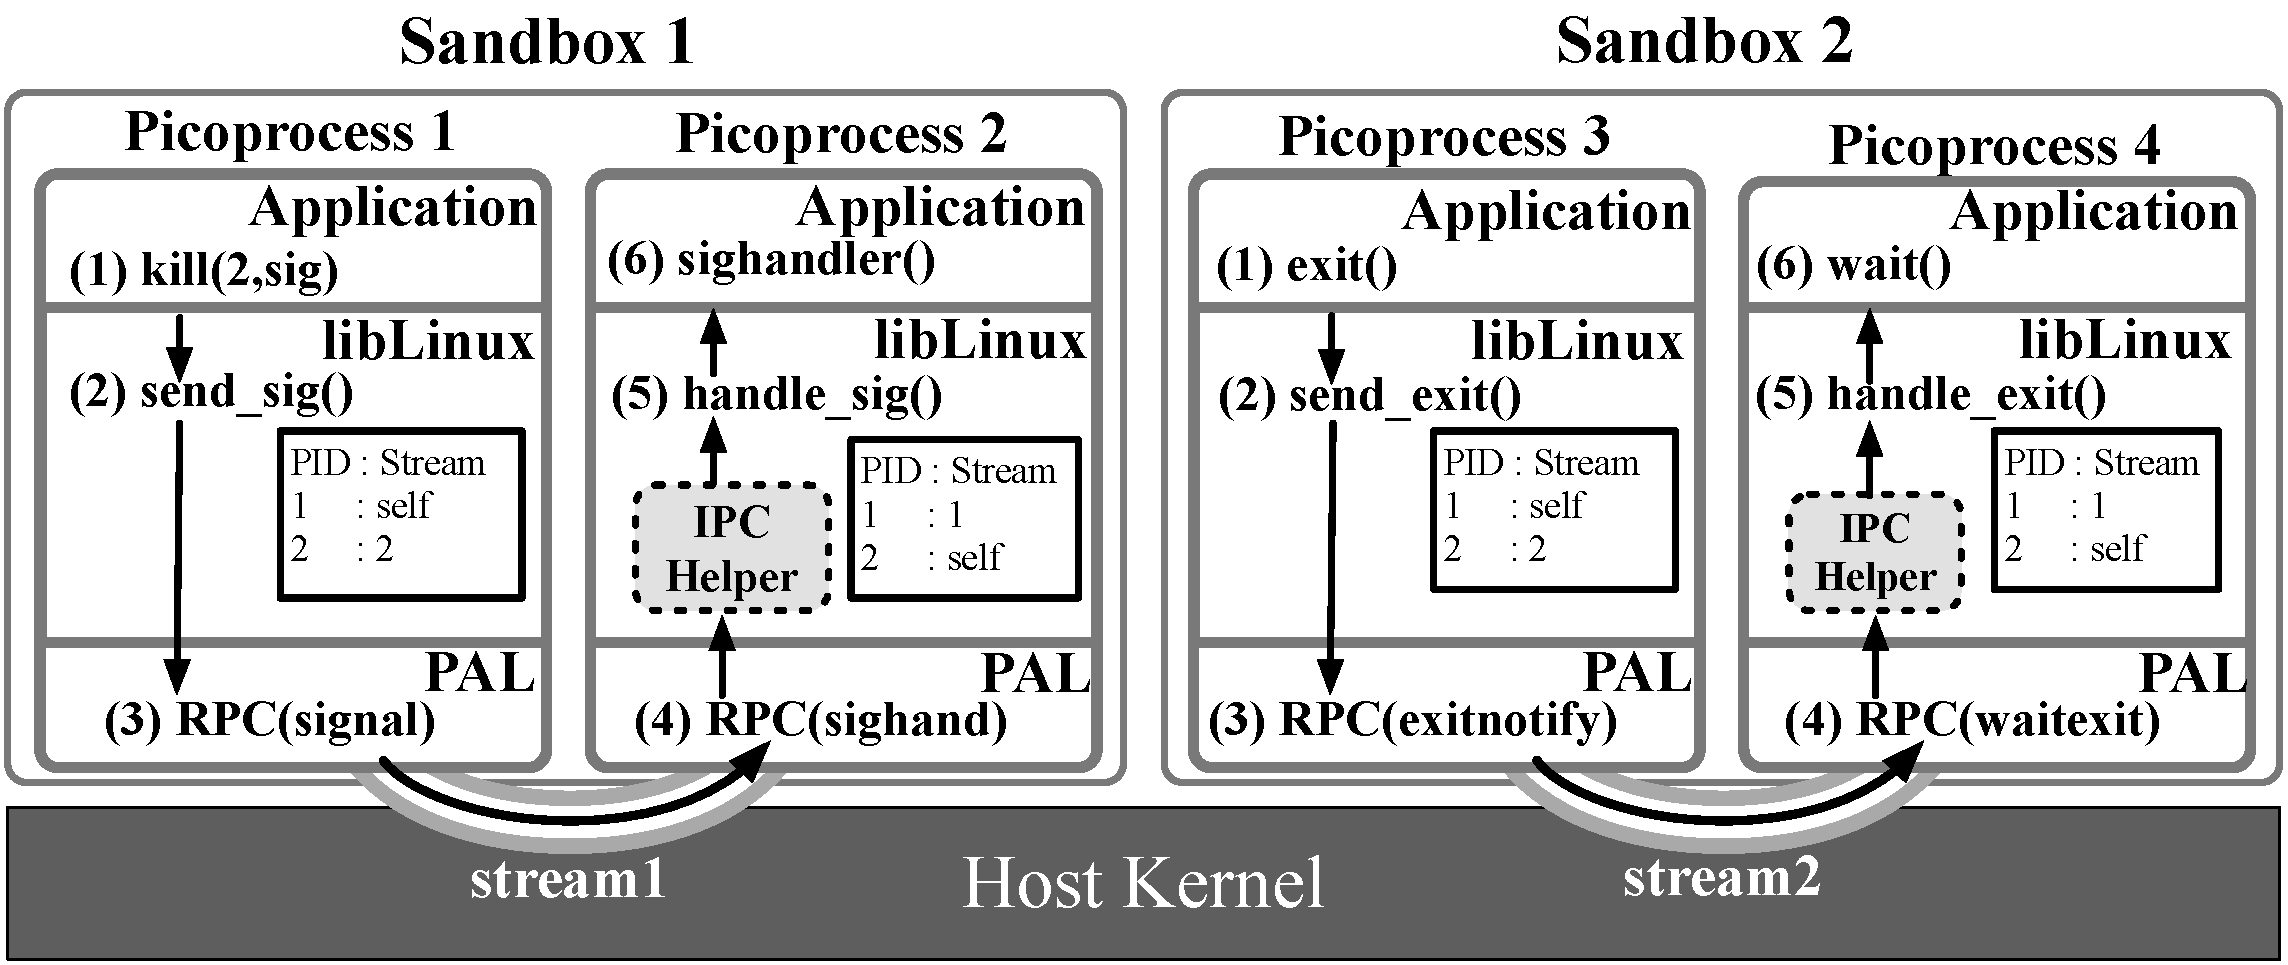
\includegraphics[width=\linewidth]{graphene/figures/coordination.pdf}
\caption{Two pairs of \graphene{} \picoprocs{} in different sandboxes 
coordinate signaling and process ID management.
The location of each PID is tracked in {\tt libLinux}; Picoprocess 1 signals
\picoproc{} 2 by sending a signal RPC over stream 1,
and the signal is ultimately delivered using a 
library implementation of the {\tt sigaction} interface. Picoprocess 4 
waits on an {\tt exitnotify} RPC from  \picoproc{} 3 over stream 2. }
\label{fig:graphene:coordination}
\end{figure}

Figure~\ref{fig:graphene:coordination} illustrates two sandboxes with \picoprocs{}
collaborating to implement a process ID (PID) namespace.  
Because PIDs and signals are a \libos{} abstraction,
\picoprocs{} in 
each sandbox can have overlapping PIDs, and
cannot signal each other.
Picoprocesses in different sandboxes cannot 
exchange RPC messages or otherwise communicate.
%If the connection between \picoprocs{} 1 and 2 is severed by subdividing the sandbox,
%the processes will become inaccessible to each other
%and each newly isolated library OS will treat the event as a process termination.


If \picoproc{} 1 (PID 1) sends a {\tt SIGUSR1} to \picoproc{} 2 (PID 2), illustrated in Figure~\ref{fig:graphene:coordination},
the {\tt kill} call to {\tt libLinux} will check its cached mapping of PIDs to 
point-to-point streams.
If {\tt libLinux} cannot find a mapping, it may begin by sending a query to the leader
to find the owner of PID 2,
and then establish a coordination stream to \picoproc{} 2.
%The leader may also pass a point-to-point coordination stream handle.
Once this stream is established, \picoproc{} 1 can send a  
signal RPC to \picoproc{} 2 (PID 2).
When \picoproc{} 2 receives this RPC, 
{\tt libLinux} will then query its local {\tt sigaction} 
structure and mark {\tt SIGUSR1} as pending.
The next time \picoproc{} 2 makes a {\tt libLinux} call,
the {\tt SIGUSR1} handler will be called upon return. Also in Figure~\ref{fig:graphene:coordination}, \picoproc{} 4 (PID 2) waits on 
\picoproc{} 3 termination (in the same sandbox with PID 1). When \picoproc{} 3 terminates, it invokes the library implementation of exit, which issues
an {\tt exitnotify} RPC to \picoproc{} 4.
%In this example, \picoprocs{} in different sandboxes have the same PID number, but this does not cause conflict as they are isolated and can only communicate with processes in the same sandbox.

%%% Using a helper thread alongside each process to asynchro-
%%% nously handle signaling
%%% is common in many \microkernel{}-based OSes such as GNU Hurd~\cite{hurd}.
%%% GNU Hurd also maintains local mappings of PIDs and RPC ports for inter-process messaging.
%%% However, PID namespace in GNU Hurd is only tracked between the parents/children, so signaling cannot be transferred between arbitrary processes.
%%% \graphene{} handles PID namespace with global consistency inside a sandbox,
%%% but requires no intensive RPCs to any centralized service.   

The \graphene{} {\tt libLinux} signal semantics closely match Linux behavior, which
delivers signals upon return from a system call or an interrupt or trap handler (\pal{} upcall).
%Each process and thread have {\tt sigaction} structures adapted from the Linux source 
%that implement the
%POSIX specification, including handler functions, as well as masking signals and
%reentrant behavior.
The {\tt libc} signal handling code is unmodified on \graphene{}.
%We extend the \pal{} with ABIs for explicit upcalls on certain hardware exceptions, such
%as divide-by-zero or segmentation faults.
%Signals from other processes, such as {\tt SIGUSR1}, are generally delivered upon 
%return from a call into {\tt libLinux}; 
If an application has a signal pending for too long,
e.g., the application is in a CPU-intensive loop, {\tt libLinux} can use a \pal{} function to interrupt 
the thread. 


% Daniela Oliveira commented. old caption for coordination
%\caption{\graphene{} namespace coordination example.  
 % Two applications and {\tt libLinux} instances
 % coordinate signaling and process ID management.
 % The location of each PID is tracked in {\tt libLinux};
 % a signal message is sent over a host stream
 % using the {\tt action} message, 
 % and the signal is ultimately delivered using a 
 % library implementation of the {\tt sigaction} interface.
%}


\begin{comment}
\graphene{} internally indexes point-to-point handles using PIDs.
In order to facilitate reallocation of PIDs without global coordination, 
\graphene{}-internal PIDs also include a {\em generation number},
allowing \picoprocs{} to lazily detect reuse similar to generation numbers 
for inodes in NFS~\cite{sandberg85nfs}.
\end{comment}

\paragraph{System V IPC.} System V IPC
maps an application-specified key onto a unique identifier.
All System V IPC abstractions, including message queues and semaphores,
are then referenced by this identifier (ID).
Similar to PIDs, 
%In order to service IPC requests, including identifier creation, from local state,
the leader divides the ID space among the \picoprocs{}, so that any \picoproc{}
can allocate an ID from local state. %a pre-allocated range.
The leader also dynamically allocates keys to \picoprocs{}.
%%% Global coordination is required to ensure that the same key maps to the same queue ID;
%%% the leader caches this information, but the owner of the queue ID or the semaphore ID 
%%% makes the definitive decision about whether a ID mapping is still valid.
%%% A key which does not have a valid mapping can be assigned to an ID by any \picoproc{}.

\paragraph{Message Queues.} In \graphene{}, the owner of a queue ID is responsible for 
storing the messages written to the queue; all message sends and receives must 
go through the owning \picoproc{}.  
In our initial implementation, any sends to or receives from a remote queue were several
orders of magnitude slower than an access to a local queue.
This led to two essential optimizations.  
First, sending to a remote
message queue was made asynchronous.  In the common case, the sender can simply assume 
the send succeeded, as the existence and location of the queue have already been determined.
The only risk of failure arises when another process deletes the queue.
When a queue is deleted, the owner sends a deletion notification to all other \picoprocs{}
that previously accessed the queue.
If a pending message was sent concurrently with the deletion notification 
(i.e., there is an application-level race condition), 
the message is treated as if it were sent after the deletion and thus dropped.
The second optimization migrates queue ownership from the producer to the consumer,
which must read queue contents synchronously.

%\fixmedp{bill: it is referenced in the Semaphores section, but here there isn't any talk about migrating msg queues to the most active \picoproc{}. also, the section starts with ``two essential optimizations. First \ldots'', but there isn't a second. is queue ownership migration the second?}

Because non-concurrent processes can share a message queue,
our implementation also uses a common file naming scheme to serialize message queues to disk.
If a \picoproc{} which owns a message queue exits, 
any pending messages are serialized to a file,
and the receiving process may request ownership of the queue from the leader.
%In order to prevent happens-before violations in case of failure, 
%message queues may be checkpointed more aggressively.


%\paragraph{Failure Recovery.}
%\label{sec:namespaces:failurerecovery}
%The \graphene{} coordination protocols are designed such that the leader does not store any unrecoverable information---the leader
%only caches the current name allocations.
%Because we assume that \picoprocs{} within a sandbox trust each other, 
%a new leader can simply broadcast a request to 
%recreate the current name allocations.  
%If the leader crashes, a simple leader election protocol is sufficient, e.g., picking the smallest live PID.

%\daniela{I wonder if the remainder of this section should be part of implementation details(section 5)}

\paragraph{Semaphores.} IPC semaphores 
follow a similar pattern to message queues, where ownership of a given semaphore is migrated
to the \picoproc{} that most frequently acquires the semaphore.
%If the owner of a semaphore exits, \graphene{} transfers ownership to the leader.  rather than serialize the semaphore to disk.
Most of the overhead in the Apache benchmark (\S\ref{sec:graphene:eval:perf}) is attributable to semaphore overheads.
%and, in ongoing work, we will likely optimize this by 
%either expanding the host ABI to share synchronization primitives within a sandbox,
%using shared memory to reduce semaphore latency.

\paragraph{Shared File Descriptors.} 
Open handle descriptors in the \graphene{} host ABI do not include a seek pointer; 
Unix-style seek behavior is implemented in the library OS.
The default Linux behavior is that children copy the open handles and file seek cursors,
but subsequent cursor movements are not shared between parent and child.
Shared file descriptor table can be requested by passing the {\tt CLONE\_FILES} flag to the {\tt clone} system call.
Any new file descriptor opened in a shared table will be visible by every process cloned in this way, as well as subsequent cursor update.
%None of our target applications have required a shared seek cursor, and it is not currently implemented,
%but would be a straightforward extension to current RPC mechanisms.
%We expect that the current RPC mechanisms could easily be extended to synchronize a seek pointer among \picoprocs{}.
If multiple \picoprocs{} are sharing file descriptor table,
the oldest one will coordinate the mapping of each file descriptor to the child \picoproc{} who owns the seek pointer.
Every update to the seek pointer will require coordination
if the \picoproc{} isn't owning it,
and similar optimization using migration can be applied here. 

\paragraph{File System States.} 
In some cases file system states need to be shared across \picoprocs{},
but the host ABI cannot export the result of Linux-specific behaviors.
For example, Linux allows user to perform specialized operations on file system
such as opening a FIFO, binding a domain socket, creating a symbolic link,
or atomically locking a file.
Coordinating these states can be cause significant slowdown on regular file system operations, so we simply export the state in regular files on the host,
 and atomically update them by renaming.

\paragraph{Shared Memory.} The \graphene{} host ABI 
does not currently permit shared memory among \picoprocs{}.
We expect that a host ABI and existing support for coordinating System V IDs would be sufficient to implement this,
with the caveat that the host must be able to handle sandbox disconnection gracefully, perhaps converting the pages to copy-on-write.
Thus far we have avoided the use of shared memory in the {\tt libLinux} implementation, both to maximize flexibility in placement of \picoprocs{}, potentially on different physical machines,
and as a rough mechanism to keep all coordination requests explicit.
%As discussed with semaphores, shared memory may also be useful to reduce latency for RPCs among picoproceses when 
%all \picoprocs{} are on the same host.


%in \graphene{} are implemented by a simple producer-consumer model.
%%% Without blocking, the latency of an inter-process semaphore operation equals to a round-trip of RPC messages.
%%% We observed that IPC semaphores can benefit from the same optimization
%%% used by message queues,
%%% based on asynchronous sending.
%%% However, when non-concurrent processes share a semaphore, it does not worth serializing the semaphore state to disk.
%%% When the owner of a semaphore exits,
%%% the semaphore state will be migrated to the leader,
%%% if it has a non-zero counter.
%%% IPC semaphores are intensively used in Apache web servers with a multi-process model. 

 
\begin{comment}
\paragraph{Limitations.} At the time of submission,
\graphene{} does not recover from all cases where a leader \picoproc{} crashes.
Our current prototype requires the IPC helper thread in the leader to remain 
in the sandbox and respond to messages even if its process {\tt main} routine has completed,
and the evaluation data reflects this state.
\end{comment}

\paragraph{Failure and Disconnection Tolerance.}  
\graphene{} is designed to tolerate disconnection of collaborating \libos{} instances,
either because of crashes or blocked RPCs.  In general, \graphene{} makes 
these disconnections isomorphic to a reasonable application behavior,
although there may be some edge cases that cannot be made completely transparent to the application.

In the absence of crashes, placing shared state in a given \picoproc{} introduces the risk that an errant 
application will corrupt shared \libos{} state.  The \microkernel{} approach of 
moving all shared state into a separate server process is more resilient to this problem.
Anecdotally, \graphene{}'s performance optimization of migrating ownership to the process that 
most heavily uses a given shared abstraction also improves the likelihood that only the corrupted
process will be affected.  
Making \graphene{} resilient to arbitrary memory corruption of any \picoproc{} is left for future work.


\paragraph{Leader Recovery.}
\graphene{} provides a leadership recovery mechanism when a leader failure is detected.
A non-leader \picoproc{} can detect the failure of a leader by either observing the shutdown of RPC streams or timing out on waiting for responses. 
Once the \picoproc{} detects leader failure, it sends out a message on the broadcast stream to volunteer for leadership.
After a few rounds of competition, the winning \picoproc{} becomes the new leader and recover the namespace state by recollecting from every other \picoproc{} in the sandbox.

%After a \picoproc{} being elected as the leader,
%the leader state,
%including all the allocated IDs and the RPC stream addresses,
%must be recovered. 
%Recollecting the leader state from all the \picoprocs{} is possible
%but can be inefficient,
%given the new leader may not have knowledge about every \picoproc{}.
%To simplify the implementation,
%we make the leaders of a namespace periodically serialize their states to disk for later recovery.

%When a \picoproc{} is sandboxed, it will detect the failure of leader because all of its RPC streams are closed by the reference monitor.
%Once it starts the leadership recovery, it will automatically win because no other \picoproc{} is sharing the broadcast stream. The procedure can be skipped by informing the sandboxed \picoproc{} before detaching.

\subsection{Lessons Learned}
\label{sec:graphene:namespaces:insights}

The current coordination design is the product of several iterations, which began 
with a fairly simple RPC-based implementation. %, and was then refined based on profiling.
This subsection summarizes the design principles that have emerged from this process.
%We present high-level facets of the design along with the insight
%behind the decision.  The next subsections synthesize these aspects 
%with specific examples of signaling and message queues.

\paragraph{Service requests from local state whenever possible.}
Sending RPC messages over Linux pipes is expensive;
this is unsurprising, given the long history of 
work on reducing IPC overhead in microkernels~\cite{liedtke93sosp,chen93memory}.  
We expect that \graphene{} performance could be improved on a 
\microkernel{} with
a more optimized IPC substrate, such as L4~\cite{liedtke95sosp,klein09sel4,elphinstone13microkernels};
we take a complementary approach of avoiding IPC if possible.
%but this is beyond the scope of our work, and we want \graphene{} to perform well on any 
%host OS.

An example of this principle is migrating message queues to the ``consumer'' when a 
clear producer/consumer pattern is detected, or migrating semaphores to the most frequent requester.
In these situations, synchronous RPC requests can be replaced with local function calls, improving
performance substantially.  For instance, migrating ownership of message queues 
reduced overhead for message receive by a factor of $10\times$.

\paragraph{Lazy discovery and caching improve performance.}  
No library OS keeps a complete replica of all distributed state,
avoiding substantial overheads to pass messages replicating irrelevant state.
Instead, \graphene{} incurs the overhead of discovering the owner of a name
on the first use, and amortizes this cost over subsequent uses.
Part of this overhead is potentially establishing a point-to-point stream,
which can then be cached for subsequent use.
For instance, the first time a process sends a signal, the helper thread 
must figure out whether the process id exists, to which \picoproc{} it maps,
and establish a point-to-point stream to the \picoproc{}.
If they exchange a second signal, the mapping is cached and reused, amortizing this 
setup cost.  For instance, the first signal a process sends to a new processes
takes \~{}2ms, but subsequent signals take only \~{}55 \us{}.

\paragraph{Batched allocation of names minimizes leader workload.}
In order to keep the leader off of the critical path of operations like {\tt fork}, 
the leader typically allocates larger blocks of names, such as process IDs or System V queue IDs.
In the case of {\tt fork}, if a \picoproc{} creates a child, it will request a batch of 
PIDs from the leader (50 by default).  Subsequent child PID allocations will be made from the same 
batch without consulting the leader.
Collaborating processes also cache the owner of a range of PIDs, avoiding 
leader queries for adjacent queries.

%% dp: Sad to see this go, but it is sort of subsumed by the other discussion
\paragraph{The coordination within a sandbox is often pairwise.}
\graphene{} optimizes the common case of pairwise coordination,
by authorizing one side of the coordination to dictate the abstraction state,
but also allows
more than two processes to share an abstraction.
Based on this insight, 
we observe that {\em not all shared state need be replicated by all \picoprocs{}}.
Instead, we adopt a design where one \picoproc{} is authoritative for a given name (e.g., a process ID or a System V queue ID).
For instance, all possible thread IDs are divided among the collaborating \picoprocs{},
and the authoritative \picoproc{} either responds to RPC requests for this thread ID (e.g., a signal)
or indicates that the thread does not exist.
This trade does make commands like {\tt ps} slower, 
but optimizes more common patterns, such as waiting for a child to exit.

\paragraph{Make RPCs asynchronous whenever possible.} 
For operations that must write to state in another \picoproc{}, 
the \graphene{} design strives to cache enough information in the sender 
to evaluate whether the operation will succeed, thereby obviating the 
need to block on the response.  This principle is applied to lower the overheads
of sending messages to a remote queue.


%this is a mapping to a thread within a specific \picoproc{}; for a message queue key,
%the mapping might be empty if the queue does not exist, or it may point to the \picoproc{} storing the pending messages.
%% The general problem underlying each of these coordination APIs is 
%% {\bf namespace management}.  In other words, coordinating \picoprocs{} need a consistent mapping
%% of names, such as a thread ID or System V message queue ID, to the authoritative \picoproc{} for that abstraction, if one exists.


\paragraph{Summary.}
The current \graphene{} design minimizes the use of RPC,
avoiding heavy communication overheads in the common case.
This design also allows for substantial flexibility to dynamically moving processes out of
a sandbox.  Finally, applications do not need to select different 
library OSes {\em a priori} based on whether they are multi-process or single-process---\graphene{}
automatically uses optimal single-process code until otherwise required.

\section{Isolating Mutually Untrusting Applications}
\label{sec:graphene:security}

\sysname{} ensures that mutually untrusting applications 
cannot interfere with each other, providing security isolation
comparable to running in separate VMs.
\sysname{} reduces the attack surface exposed to applications
by restricting access to the host kernel ABI 
and prevents access to unauthorized system calls, files, byte streams,
and network addresses with a \term{reference monitor}.
%The host kernel ABI exported by the \pal{} heavily 
%limits the ability of a \sysname{} application to interact with the rest of the system;
%any external interactions are further mediated by a reference monitor.
%Unlike a typical Linux system, \sysname{} applications cannot interact with shared 
%system daemons or other shared system resources.
%As a result, \sysname{} enforces security isolation similar to running applications in separate VMs---even
%applications that span multiple processes.
\sysname{} contributes a multi-process security model 
based on the abstraction of a \term{sandbox},
or a set of mutually trusting picoprocesses.
The reference monitor permits picoprocesses within the same sandbox
to communicate and exchange RPC messages, but disallows cross-sandbox communication.
The current work focuses on all-or-nothing security isolation, although we expect
this design could support
controlled communication among mutually untrusting \liboses{}
in future work.

The only kernel-level sharing abstractions the reference monitor must mediate
are files, network sockets, and RPC streams
--- all other allowed kernel ABIs
modify only local \picoproc{} state.
%Thus, the reference monitor need only mediate file access, socket and RPC stream creation.
%an unprivileged daemon
%as well as extensions to the App\-Armor LSM~\citep{apparmor},
%which checks file and socket policies in the kernel.
%, reducing context switching overhead
%and the risk of race conditions~\citep{garfinkel03traps}.
In order for the reference monitor to restrict file access, socket and RPC stream creation,
each application includes a \term{manifest file}~\citep{hunt07rethink},
which describes a {\tt chroot}-like, restricted view of the local 
file system (similar to Plan 9's unioned file system views~\citep{pike90plan9}),
%including read-only shared files,
as well as \term{iptables}-style~\citep{iptablesman} network restrictions.
%%% To facilitate sharing read-only libraries,
%%% a manifest may specify a file system view which 
%%% combines several different sub-directories of the local file system,
%%% and can prevent writing to files or directories.


%The \sysname{} reference monitor on a Linux host
%is implemented using {\tt ioctl} system call to a special device {\tt /dev/graphene}.
%A picoprocess is restricted by seccomp filter~\citep{seccomp} to use any {\tt open} or socket {\tt connect} and {\tt bind} system calls.
%It must use the \sysname{} special device to open or create streams,
%so the file paths or network addresses can be checked against the sandbox rules.
%The kernel module as the driver of the \sysname{} special device can coexist with any LSM such as \term{AppArmor} or \term{SELinux}.


\fixme{Explain with a figure.}
When a new picoprocess is launched by the reference monitor, it begins execution in 
a new sandbox.  
Child picoprocesses may either inherit their parent's sandbox, 
or can be started in a separate sandbox
--- specified by a flag to the picoprocess creation ABI.
A parent may specify a subset of its own file system view 
when creating a child, but may not request access to new regions of the 
host file system. 
%The restrictive policy enforced on the child will be written in a new manifest file generated by the parent, and the policy will be checked by the reference monitor.
The child may also issue an {\tt ioctl} call to 
dynamically detach from the parent's sandbox. The reference monitor prevents byte stream creation 
across sandboxes.
%among picoprocesses
%that are not in the same sandbox.
%and restricts external connections to remote URIs according to firewall rules in the manifest.
When a process detaches from a sandbox --- effectively splitting the sandbox ---
the reference monitor closes
any byte streams that could bridge the two sandboxes.

\paragraph{Threat Model.}
We assume  a trustworthy host OS and reference monitor,
which mediates all system calls with effects outside of a picoprocess's address space,
such as file {\tt open} or network socket {\tt bind} or {\tt connect}.
We assume that picoprocesses inside the same sandbox trust each other and that all untrusted code runs in sandboxed picoprocesses.
We assume the adversary can run arbitrary code inside of
one or more picoprocesses within one or more sandboxes.
The adversary can control all code in its
picoprocesses, including {\tt libLinux} and the \pal{}. 
%We also assume a trusted reference monitor process running on the host kernel that 
%launches \sysname{} applications and mediates all system calls with external effects,\fixmedp{define precisely}

\sysname{} ensures that %The key security property the \sysname{} design upholds is that 
the adversary cannot interfere with any victim picoprocesses
in a separate sandbox.  
The \sysname{} sandbox design ensures strict isolation: 
if the only shared kernel abstractions are byte streams and files, 
and the reference monitor ensures
there is no writable intersection between sandboxes,
the adversary cannot interfere with any victim picoprocess.


%%% The only processes allowed to run as standard kernel processes (non-\sysname{}) 
%%% are the reference monitor and
%%% system administration utilities that need more kernel interfaces than the \pal{} ABI provides.
%%% Ensuring that a collaborating picoprocess correctly implements
%%% some function (such as receiving a signal),
%%% as well as preventing exploitation of vulnerabilities in picoprocesses
%%% are beyond the scope of this work.

\sysname{} reduces the system attack surface of the host, but does not change the size of its
trusted computing base; however, reducing the effective system call table
size of a picoprocess does facilitate adoption of a smaller host kernel,
which we leave for future work.

\subsection{System Call Restriction}
\label{sec:graphene:security:syscalls}


Unmodified Linux applications run on \sysname{} by issuing 
system calls as library calls to {\tt libLinux}.
Application calls are serviced by {\tt libLinux}-internal data structures
or \pal{} calls.
The \pal{} is implemented using \nativecalls{} host system calls.
The host OS must block any 
native system call that 
does not appear in the \pal{} source code.
Any allowed system call with external effects is checked by 
the reference monitor.
 
%% dp: Meh
%%% Any picoprocess implementation 
%%% must restrict access to the host system call table,
%%% generally by blocking system calls in the host kernel~\citep{porter11drawbridge}
%%% or using {\tt ptrace}~\citep{xax}.


%The \pal{} is a host-provided library which implements \palcalls{} generic kernel ABIs,
%implemented using 
%These native system calls include {\tt ioctl} with 5 opcodes exclusively used by \sysname{} kernel extensions.

%This section describes how we adapt recent Linux sandboxing techniques 
%to \sysname{}.


%all allowed system calls with potentially external effects.

%%% For instance, an attempt to open a file will be checked by the reference monitor
%%% to see if the file is included in the sandbox definition, specified in the manifest
%%% with required permissions.
%%% Once the file handle is open, the \pal{} is then allowed to issue an {\tt mmap} or {\tt read}
%%% on the handle, as this operation can only affect the picoprocess address space
%%% or  file, which was already checked.

%Because the \pal{} is in the same address space as the application code, it is not
%trusted to enforce any security policies, and our threat model assumes that
%the \pal{} can be compromised by the adversary.
%Thus, the host kernel 
%only permits system calls that appear in the \pal{}'s source code and, through the reference monitor, further inspects calls that can have external effects.

\begin{figure}[t!]
\centering
\includegraphics[width=6.5in]{graphene/figures/syscall-restriction.pdf}
\footnotesize
\caption[System call restriction approach in sysname{}]
{System call restriction approach. The reference monitor loads policies into the LSM at startup.  A \sysname{} application requests OS services in three different ways. 
In the normal case (first line of {\tt main}), {\tt malloc} is invoked causing the invocation of {\tt brk} ({\tt libLinux}) and {\tt mmap} in the \pal{}. In the second line, the application jumps to an address in \pal{}, which is permissible.
Files are accessed through {\tt ioctl} to {\tt /dev/graphene} and checked by reference monitor.
The third line invokes {\tt brk} with an {\tt int} instruction, which is redirected to the {\tt libLinux} function.}
\label{fig:graphene:syscall-restriction}
\end{figure}



\sysname{} restricts the host system call table 
using seccomp~\citep{seccomp}, introduced in Linux 2.6.12.
% a recent Linux system call filtering mechanism, called 
Seccomp allows a process to create an immutable Berkeley Packet Filter (BPF) program
that specifies allowed system calls, as well as creates {\tt ptrace} 
events on certain system calls.
The filter can also filter scalar argument values,
such as only permitting specific {\tt ioctl} opcodes.
%The BPF grammar is rich enough to filter system calls by 
%This feature is particularly salient in the case of {\tt ioctl},
%where the \pal{} uses 5 out of over 400 opcodes for our bulk IPC module and sandbox creation;
%our BPF rules will block any other {\tt ioctl} opcode.
If a system call is rejected, the \pal{} will receive a {\tt SIGSYS} signal,
and can either terminate the application or redirect the 
call to {\tt libLinux}.
Seccomp filters cannot be overridden by any picoprocess,
and are always inherited.
% by all descendant processes.
The current \sysname{} filter is 79 lines 
of straightforward BPF macros.  In our experience, adding more precise argument checks
has not significantly changed performance.

%Seccomp filters are installed using the {\tt prctl} system call;
%blocking {\tt prctl} in a seccomp filter prevents further changes to the filter.

Unfortunately, the logic to check for allowed paths network addresses cannot be implemented 
as a seccomp rule, because it involves reading user memory of unknown sizes. 
In order to avoid the overhead of trapping to the reference monitor on 
every use of {\tt open}, {\tt stat}, {\tt bind} or {\tt connect} system calls, we instead 
force picoprocess to only use {\tt ioctl} system call to \sysname{} special device ({\tt /dev/graphene}) as alternative interface these system calls. Direct access to these system calls are banned by seccomp filter.
%extend AppArmor~\citep{apparmor} 
%to enforce file system isolation in the kernel.

In order to reduce the impact of bugs in the reference monitor,
the reference monitor itself runs with a seccomp filter,
blocking unexpected system calls.

\paragraph{Static Binaries.} 
For compatibility with statically linked binaries, which 
compile in system call instructions,
we leverage seccomp to redirect these calls 
back to {\tt libLinux}.  
For system calls that could also be issued by the \pal{},
we augment our BPF rules with program counter-based filters.
In other words, an {\tt open} system call with a return PC address inside the \pal{} 
will be sent to the reference monitor for further inspection;
an {\tt open} system call with any other return PC address generates 
a {\tt SIGSYS} and is ultimately relayed back to {\tt libLinux}.
Thus, {\tt libLinux} can catch and differentiate application-issued system calls
from those that could also be issued by the \pal{}.
We hasten to note this feature is only for backward compatibility,
not security. 


\begin{comment}
We hasten to note that program counter filtering
is only provided for backwards compatibility, not security.
An attacker can compromise the \pal{}, so system policies are enforced
externally by the reference monitor.


Dynamically redirecting system calls to {\tt libLinux} is 
less efficient than dynamically linking against
the \sysname{} libc or statically compiling {\tt libLinux} into the application.
The overhead of dynamic redirection comes from 
transferring control to the kernel, then back to 
the \pal{}, and then to {\tt libLinux}.
We leave exploration of more efficient alternatives for future work,
such as redirecting the hardware system call table to {\tt libLinux}
on a host system like Dune~\citep{belay12dune},
or dynamically rewriting parts of the static binary~\citep{hunt99detours}.
\end{comment}

\paragraph{Example.}
Figure~\ref{fig:graphene:syscall-restriction} illustrates three possible situations. 
%% An unmodified Linux application is dynamically linked against the 
%% \sysname{} {\tt libc}, 
%% which then dynamically links its system calls from {\tt libLinux},
%% which in turn links in the host kernel ABI from the \pal{}.
%% The application requests OS functionality in three ways.
An unmodified application first invokes the {\tt libc} function {\tt malloc}, which issues 
a {\tt brk} system call to {\tt libLinux}, which requests memory 
from the host via a {\tt Dk\-Virtual\-Memory\-Alloc} \pal{} call,
which ultimately issues an {\tt mmap} host system call.
The {\tt mmap} host system call is allowed by seccomp because it only 
affects the picoprocess's address space.
The second line of the application jumps to the \pal{} instruction that issues
an {\tt open} system call.
From a security perspective, this is permissible,
as it is isomorphic to \pal{} functionality.
In practice, this could cause
corruption of {\tt libLinux} or application data structures,
but the only harm is to the application itself. 
Because this system call involves the file system, the reference monitor LSM first checks if the file to be opened is included in the sandbox definition (manifest) before allowing  the {\tt open} system call in the kernel.  
Finally, the application uses inline assembly to issue a {\tt brk} system call;
%in an attempt to obtain I/O port privilege; 
because this system call was not issued by the \pal{},
seccomp will redirect this call back to the \pal{},
which then calls the {\tt libLinux} implementation.

\paragraph{Process-specific Isolation.} 
Sandbox creation in \sysname{} can provide
more options than virtualization, to reflect the security policy of applications at any timing,
in the granularity of picoprocess. 
A picoprocess can voluntarily detach itself from the current sandbox, dropping its privileges,
after finishing security-sensitive operations.
If a picoprocess decides one of its children is not trustworthy, it may also start the child under a restricted manifest,
or promptly shut down RPC streams to stop sharing OS states.
The picoprocess that moves to a separate sandbox will have a restrictive view of the filesystem, and no coordination with the previous sandboxes.
In section~\ref{sec:graphene:eval}, we describe an experiment that improves security isolation of Apache web server without sacrificing functionality.

\subsection{Reference Monitor}
\label{sec:graphene:security:monitor}

The reference monitor is a trusted process that runs on the host system.
\sysname{} applications are launched by the reference monitor,
which instantiates the seccomp filter and traces all children
to check host system calls that could have external effects.
The reference monitor interposes using ptrace events, 
which can be raised for specific system calls by seccomp.
We ensure that all processes created within a sandbox are traced
by setting the {\tt PTRACE\_O\_TRACESECCOMP} option on all newly created picoprocesses
in the sandbox.

%% from bpjain:
% We have to set the option PTRACE\_O\_TRACESECCOMP on new children
% using ptrace(PTRACE\_SETOPTIONS) and we get the event as
% PTRACE\_EVENT\_SECCOMP whenever a syscall that is Traced is called.
% It happens before the grandchild starts running. We get the
% notification of creation of grandchildren by setting ptrace option
% PTRACE\_O\_TRACECLONE on the child(i.e., parent of grandchild).  I
% need to monitor every fork/clone (only clone since pal only calls
% clone). I get this event even if fork/clone is just allowed.  And
% the event that arrives on clone/fork is completely different from
% seccomp event. Thats a ptrace event too.. but we get
% PTRACE\_EVENT\_CLONE whenever a clone is done by a child on which
% PTRACE\_O\_TRACECLONE option was set.

Each application includes a \term{manifest file}, which specifies restrictions,
including network firewall rules and subsets of the host file system sandboxed
applications are permitted to access.  The reference monitor enforces these
rules by interposing on all system calls involving file paths or remote network addresses.
%\fixmedp{Revise if we can do something smarter; 2x check implementation status before submission}.

%% dp Sadface :(
\paragraph{Privilege.~} 
Although the reference monitor is trusted, it does not run 
with administrative privilege.
Linux 3.5, which we use as our host kernel, 
introduced the {\tt NO\_NEW\_PRIVS} bit, which permits
a non-privileged process to impose sandboxing restrictions on a child.
%Ubuntu back-ported this feature to Linux 3.2, which we use as our host kernel.
This flag prevents a process from acquiring root privilege, % (e.g., via executing a {\tt setuid} binary),
is inherited by all descendant processes,
and cannot be disabled.

\paragraph{Creating New Sandboxes.~} We add a \pal{} call which
permits a picoprocess to request that it be moved into a new sandbox.
This call, as well as file system path checks, are implemented
as extensions to the  AppArmor LSM~\citep{apparmor}.
%We modify \sandboxmodlines{} lines in the
%to implement this call,
The new sandbox call closes any open stream handles that cross sandbox boundaries;
mediate path lookups;
and create a new broadcast stream for multi-process
 coordination (\S\ref{sec:graphene:namespaces:blocks}).
%The reference monitor also interposes on this call so that it can 
%mediate future stream creation.

To securely apply seccomp filtering we leveraged the fact that all
\sysname{} processes have the same parent and also the new
{\tt NO\_NEW\_PRIVS} bit introduced for Linux processes starting kernel
version 3.5. This bit can be set by any process, is inherited across
{\tt fork}, {\tt clone}, and {\tt execve}, and cannot be unset by
children processes. Thus, we set the {\tt NO\_NEW\_PRIVS} bit in the initial
\sysname{} process and apply seccomp filters allowing only system calls
with corresponding functions in the \pal{}. As a result all \sysname{}
processes will inherit the filters and cannot relax or bypass it.



%which reduces the kernel
%system call API surface to user-level processes. This mechanism allows
%a process to specify a whitelist filter for system calls, which is
%implemented as a Berkeley Packet Filter (BPF) program. The invocation
%of a disallowed system call causes the application to throw a {\tt SIGSYS}
%signal, which can be caught by a registered handler provided by the
%application. In \sysname{} we registered this handler at the \pal{}.


%\sysname{} applications rely on an OS loaded as a library to request
%system services. As most of traditional applications, \sysname{}
%processes do not normally issue system calls directly: they invoke
%wrapper functions from a \sysname{}-compliant version of libc, which
%allows for portability, security (parameters are limited and checked)
%and easiness of programming. However, while standard libc functions
%directly invoke the kernel system call themselves, our modified
%version of libc wrappers invoke functions from another library which
%represents the OS, libLinux (Figure \ref{fig:graphene:syscall-restriction}). A
%\sysname{} application can access all necessary system functionality
%through libLinux, which invokes corresponding system call functions at
%the \pal{}, also loaded as a library with a
%\sysname{} process. The \pal{} is the layer responsible for directly
%invoking system calls at the kernel. As discussed in \S\ref{sec:graphene:impl} the \pal{} provides \sysname{} applications with a
%subset of the kernel system call interface.\sysname{} applications rely
%on an OS loaded as a library to request system services.
%
%Even though we expect most of \sysname{} applications to leverage libc
%wrappers, we need to address applications that need to invoke system
%calls directly. Applications might need to bypass a library such as
%libc because some needed wrappers are not provided (there are no
%wrappers in libc for module and NUMA related system calls), or the
%wrapper does not meet the programmer’s needs. \sysname{} applications
%that need to perform direct invocation of system calls run unmodified
%as long as the system calls invoked are provided by the libos{l{}. We
%do not consider this a security violation; even though the application
%would be risking not functioning according to the libosaradigm for
%bypassing the \pal{}, all potential damage would be confined in the
%misbehaving application itself.  However, we do not allow the direct
%invocation of a system call that does not have a corresponding
%function in the libosnd \pal{}. In Figure \ref{fig:graphene:syscall-restriction}
%we illustrate these three situations. We have a \sysname{} application
%loaded with three libraries: a \sysname{}-compliant libc, libLinux
%representing the library OS with functions for a selected number of
%system calls, and the \pal{} which actually invokes host kernel system
%calls. The illustrated application requests three different types of
%OS functionality. It first invokes a function from libc, then it
%directly invokes a system call whose functionality is provided by the
%\pal{}, and third it attempts to directly invoke a system call not
%present in the \pal{}, which is not allowed by \sysname{}.

%We enforce system call restriction by leveraging seccomp Linux system
%call filtering mechanism~\citep{seccomp}, which reduces the kernel
%system call API surface to user-level processes. This mechanism allows
%a process to specify a whitelist filter for system calls, which is
%implemented as a Berkeley Packet Filter (BPF) program. The invocation
%of a disallowed system call causes the application to throw a {\tt SIGSYS}
%signal, which can be caught by a registered handler provided by the
%application. In \sysname{} we registered this handler at the \pal{}.
%
%To securely apply seccomp filtering we leveraged the fact that all
%\sysname{} processes have the same parent and also the new
%{\tt NO\_NEW\_PRIVS} bit introduced for Linux processes starting kernel
%version 3.5. This bit can be set by any process, is inherited across
%{\tt fork}, {\tt clone}, and {\tt execve}, and cannot be unset by
%children processes. Thus, we set the {\tt NO\_NEW\_PRIVS} bit in the initial
%\sysname{} process and apply seccomp filters allowing only system calls
%with corresponding functions in the \pal{}. As a result all \sysname{}
%processes will inherit the filters and cannot relax or bypass it.


%\begin{figure}
%\begin{centering}
%\includegraphics[width=2.0in\textwidth]{figures/syscall_restriction.png}
%\footnotesize
%\caption{System call restriction approach. \sysname{} application requesting OS services. The {\tt printf} function is handled by a wrapper function at our modified version of libc., which invoked a corresponding syscall function at libLinux, the library OS.This function invokes a system call function at the \pal{}, which actually invokes kernel system calls. The application also directly invokes two system calls and the last invocation is prohibited.
%\label{fig:syscall_restriction}
%\end{centering}
%\end{figure}

%\end{comment}

\section{Isolation against Untrusted Hosts}
\label{sec:graphene:sgx}

%\sysname{} is a port of \graphene{} \libos{} to \sgx{},
%to secure native Linux application in \sgx{} enclaves.
%The portability of \graphene{} is discribed in \S\ref{sec:graphene:impl}.
%\sysname{} uses the non-partitioned model
%to secure applications,
%thus only minimal effort is required for developers
%to port applications to \sysname{}.

%\graphene{} \libos{} originally runs on Linux hosts, but with the platform
%adaption layer (PAL) ported to other platform,
%\graphene{} can run Linux applications on other hosts such as
%Windows, BSD or OSX.
%\graphene{} supports up to 139 most commonly used Linux system calls
%(300 in total),
%providing reasonable Linux platform compliance.

%\section{Background and Overview}
%\label{sec:gsgx:background}

%\subsection{\intel{} \sgx{} Enclaves}
%\label{sec:graphene:background:sgx}

%\begin{figure}[t!]
%\centering
%\includegraphics[width=5in]{graphene-sgx/figures/libosvssdk.pdf}
%\footnotesize
%\vspace{-0.3in}
%\caption[Comparison between libOS-based model and partitioned model for Intel SGX]
%{Comparison between libOS-based model (e.g., \haven{} and \sysname{})
%and SDK-based (SDK for \sgx{}) model for migrating applications in enclaves.
%Green (light) boxes are trusted components and red (dark) boxes are untrusted.
%The libOS-based model often yields a larger TCB in the enclave,
%while the SDK-based model requires developers to be responsible of
%securing the enclave on the untrusted interface.}
%\label{fig:libosvssdk}
%\end{figure}

\intel{} \sgx{} (Software Guard Extension)
is a set of new x86/x86\_64 instructions
introduced in the latest \intel{} \skylake{} processors,
to create, interface and attest
an isolated memory region (\emph{enclave}) inside applications' virtual memory.
\sgx{} guarantee any data in an enclave
stay encrypted in the DRAMs, using a secret key derived from
the application's cryptographic measurements.
The secret data store in the enclave memory
can only be accessed within the code inside the enclave,
and the code must be signed by the developers' private key.
The use cases of \sgx{} mostly involve an enclave
retrieving a signed attestation from the \intel{} processor,
to exchange provisioning of information from trusted remote servers.
The purpose is equivalent to
expanding the execution from remote servers
to untrusted hosts,
to securely harness resources such as CPU cycles and DRAMs.

\sgx{} is an appealing tool for protecting small, highly sensitive execution, 
against malicious or compromised OSes, hypervisors, or even hardware peripheral.
For instance, \cite{hoekstra13sgx} show how SGX can be used
to build a trusted path from a video chat application to a GPU and network card, which maintains confidentiality and integrity of the
video stream, even if the OS is compromised.
Similarly, because DRAM contents are encrypted, SGX can resist attacks such as cold-boot attacks~\cite{halderman09coldboot} or 
malicious peripheral devices~\cite{hudson15thunderstrike}.

\paragraph{A Partitioned Usage Model.}
To secure an application with \sgx{},
the common usage model requires the developers to partition the application into two parts:
the trusted part which runs the sensitive execution in the enclave,
and the untrusted part which loads and triggers the execution of the trusted parts.
%Developers shall keep the trusted path as small and simple
%Even if the trusted code only contains the simplest the logic,
%the untrusted code is still needed to pass the input and output of the execution.
The interaction between the trusted and untrusted parts is through \emph{untrusted interfaces}.
Untrusted interfaces are defined by the developers, and include a few
logical entry and exit points of the enclave.
In the architectural level,
an enclave only has exactly one hardware entry point and one exit point.
The architecture forbids the untrusted part
to willingly jump into any location of an enclave,
to bypass or alter the valid behavior of the trusted part.
The control flow of the execution is the enclave transfers to one of the logical entry points,
based on the input parameter passed
at the hardware entry point.
%The control transfer from the hardware entry point to the logical entry points
%is based on the operation code passed as an argument at enclave entry.

With the partitioned usage model,
the developers can minimize the trusted computing base (TCB) of the enclave,
at their best effort,
and restraint the behavior of the isolated execution.
% that can only be triggered by the untrusted interface.
The partitioning prevents unpredictable behaviors in the enclave,
to compromise the confidentiality or integrity.
The developers explicitly mark the sites in the application code
to determine entry and exit of the enclave.
%The untrusted and trusted code must explicitly call for enclave entry or exit
%at the fixed sites in the application.

%\intel{} \sgx{} ({\it Software Guard Extensions})
%are a set of new x86/x64 instructions
%introduced in the \intel{} Skylake processor family.
%Using \sgx{}, an 
%application can designate part of its virtual memory as an {\em enclave}.
%The CPU guarantees that the contents of the enclave never leave the CPU package unencrypted.
%The CPU also measures the integrity of a binary loaded into the enclave, and offers remote attestation,
%similar to a TPM~\cite{TPM}.


%%% create a protected memory region, called an {\em enclave}, inside it's virtual memory,
%%% where it can load its security sensitive data with hardware-enforced isolation from the untrusted OS. 
%%% The processor with \sgx{}
%%% guarantees that any data loaded in enclave
%%% stays encrypted in the DRAM, by using a secret key deterministically derived from the application's cryptographic measurement and the CPU secret. 



% \sgx{} provides useful building blocks for secure applications, but does not
%absolve the programmer of all responsibility for reasoning about end-to-end security.
%Bugs in the application or supporting libraries can still disclose sensitive data from an enclave,
%and porting code into SGX can be subtle.
%
%Fundamentally, this argues for writing enclave code in higher-level languages
%(e.g., \java{}) that provide important 
%safety properties, such as memory and type safety, that reduce or eliminate common vulnerabilities.
%Ideally, one would formally verify security properties of enclave code~\cite{moat}; this verification is significantly aided by using 
%higher-level languages amenable to formal reasoning.  Verification is significantly harder
%with C/C++ or assembly languages.

%One must note that \sgx{} only promises the integrity of application binaries
%initially loaded in enclaves.
%The gap between integrity of binaries and complete security has to be filled
%by ones who develop and approve the applications.
%More specifically, the clients are responsible of
%testing whether the applications contain any vulnerabilities
%that lead to information leak.
%To minimize the risk of leaving any flaws in the applications unintentionally,
%developers often tend to cut down the trusted computing base (TCB)
%of the applications. With smaller TCB, clients who launched the enclaves
%can more easily reason about the thoroughness of securing the execution.

%To achieve smaller TCB, the software development kit of \sgx{}
%intends to encourage developers to partition the applications and
%keep only security sensitive components in the enclaves.
%Such an intention is exactly contradicted by the trust model of \haven{},
%which must trust the loaded application as a whole.
%Except for the cases in which the whole applications must be secured,
%\haven{} actually downgrades the trustworthiness of enclaves.
%Figure~\ref{fig:gsgx:libosvssdk} shows the comparison of the two models.

\paragraph{Using A Library OS.}
 
The partitioned usage model
restricts the risk of the isolated execution being
compromised by the untrusted host,
yet requires the developers to
cleanly split a part of the application
and inject entry and exit points at wherever interaction is needed.
Moreover, the developers are responsible
for validating and examining the soundness of the partitioned application,
to ensure every execution paths in the enclave
that are affected by the untrusted entities
are carefully checked and sanitized.
Porting a legacy application to a partitioned model
requires developers to have substantial familiarity to the application code,
as well as the principles for
developing unexploitable,
well-controlled execution in the enclave.
%be familiar with
%the mechanism of enclave entry and exit,
%and always bear the security of the isolated execution in mind.
%For developers that are not expert to architecture and security issues,
%pursuing the partitioned model may need significant efforts.   
When the sensitive execution to be isolated in the enclave
becomes considerably complex,
the effort for porting and validating the execution
quickly becomes unacceptably expensive.

\emph{Haven}~\cite{baumann14haven}
shows a \emph{non-partitioned usage model},
for loading whole, unmodified applications and supporting libraries
into enclaves.
The non-partitioned model allows application to be run in the enclave as it is, without any porting effort.
To support the non-partitioned model,
a key requirement is to support the system APIs needed by
the application and supporting libraries,
right inside the enclave.
Essentially, the execution not only is forbidden to access any host system APIs
(i.e., using {\tt syscall} or {\tt sysenter} instructions)
in the enclave,
but also unsafe to rely on the untrusted host
to provide system APIs.
A \libos{}, on the other hand, supports system APIs as in-memory function calls,
and mediates all input and output
during interaction with the untrusted host.
For instance, Haven supports unmodified Windows applications in enclaves,
using \drawbridge{} \libos{}~\cite{porter11drawbridge}
to handle all the Windows API calls.

At the low level, the non-partitioned model still requires partitioning, but instead of the applications,
it is the \libos{} itself that needs to be partitioned.
More precisely, The \pal{} that provides host ABI to the \libos{} is the component that is split across the two sides of the enclave boundary,
while the \libos{}, alone with the isolated application
and its supporting libraries,
are dynamically loaded.
The partitioned \pal{} interacts with the host through a fixed, narrow untrusted interface,
to access host resources if necessary.
%interacts with a \libos{}-specific untrusted interface,
%which is the only trusted interface needed to be defined,
%and will never be extended no matter which application is loaded.


\subsection{Porting \graphene{} to \intel{} \sgx{}}

\fixme{Need transition here}

The building blocks are shown as figure~\ref{fig:graphene:sgx-arch}.
\graphenesgx{} is partitioned into two parts:
an untrusted \pal{} to initialize the enclave and provide the untrusted interface;
and the trusted \libos{} including the host ABI, {\tt libLinux}, and core {\tt libc} libraries.
Except the host ABI is statically loaded in the enclave since the start up,
other components of \graphenesgx{} in the enclave are dynamically loaded,
as needed. 
%For each binary loaded by \sysname{}, \sysname{} bootstraps the enclave
%from an untrusted platform adaption layer (PAL) that defines
%a narrowed untrusted interface.
%To speed up initialization, the untrusted PAL starts the enclave
%with an statically linked library image ({\tt graphene.so}).
%The image includes
%\graphene{} host ABI,
%\libos{} ({\tt libLinux}, implementing Linux personality),
%and basic libraries of GNU library C
%({\tt libc}, {\tt libpthread} and {\tt ld}, the runtime loader).
%The \sysname{} library image then loads the unmodified applications
%and libraries into the enclave.
After the \libos{} is laoded in the enclave,
the \libos{} will load the application and its supporting libraries,
and call their entry functions.
The \libos{} will handle all the system calls redirected from the applications,
whereas it may access host resource through the host ABI calls,
which are redirected to the untrusted interface
to interact with the host. 

\begin{figure}[t!]
\centering
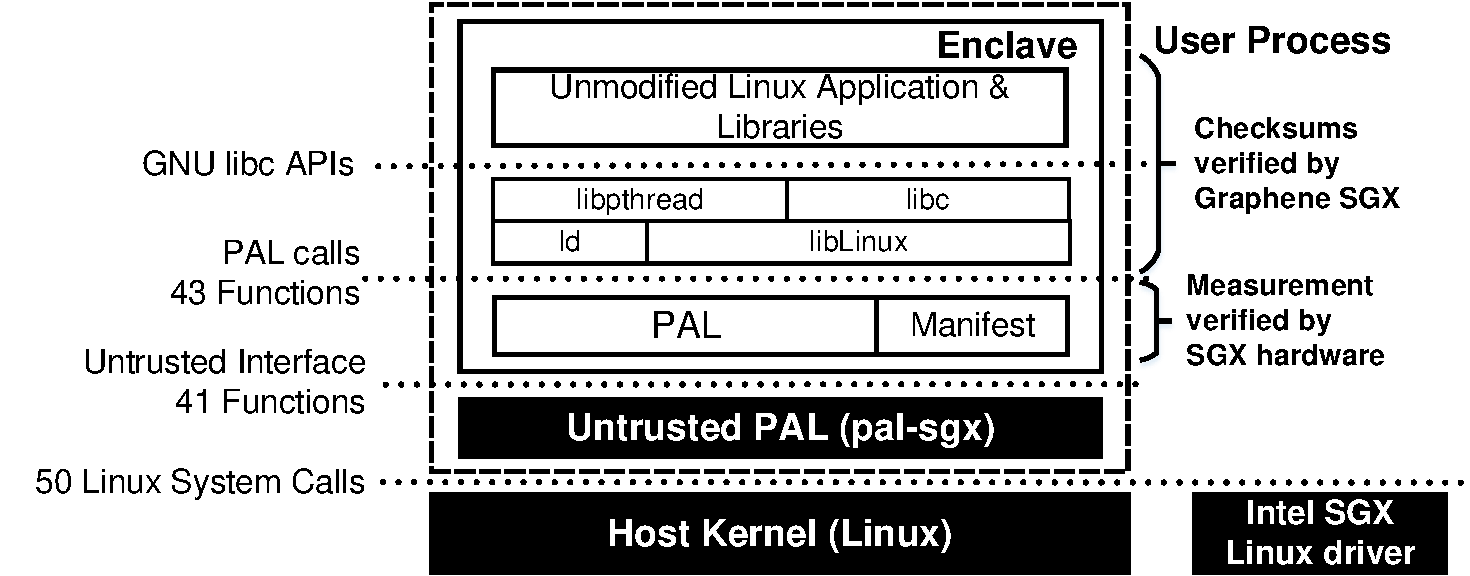
\includegraphics[width=5.5in]{graphene-sgx/figures/architecture.pdf}
\footnotesize
\caption[The \graphenesgx{} building blocks]
{The \graphenesgx{} building blocks.
Green (light) boxes are trusted components trusted,
and red (dark) boxes are untrusted.
\graphenesgx{} is statically linked with {\tt libLinux},
the \libos{} binary, and basic libraries of GNU library C.
To build up the trust, the \graphenesgx{} image along with
a manifest and application measurements
are verified by \sgx{} during bootstrap. Applications and other libraries
are verified by \graphenesgx{}. The enclave interacts with the host kernel,
through untrusted PAL, on a narrowed untrusted interfaces with 41 functions.}
\label{fig:graphene:sgx-arch}
\end{figure}

\paragraph{Applications Integrity.}
A key requirement of the non-partitioned usage model is to guarantee the integrity of the secured applications.
Because the applications are dynamically loaded by the \libos{}
{\em after} the enclave starts up,
the CPUs cannot verify the integrity of loaded application binaries.
An alternative is to place all application binaries in an encrypted virtual disk,
which can be decrypted using a securely provisioned key~\cite{baumann14haven}.

\graphenesgx{} guarantees the integrity of applications
by signing each supporting binaries or generating checksums for the binaries.
For each secured application, the signing tool will generate
a manifest and a correspondent signature.
A manifest will contain the attributes of the enclave and \libos{},
and the checksums of the supporting binaries.
The manifest will be loaded in the enclave before the enclave starts,
and verified by the hardware as part of the enclave measurement.
The integrity of the supporting binaries
are validated by \pal{} before loading from the untrusted host.

By verify the integrity of applications individually,
we decouple the deployment and verification of the application binaries;
users may simply deploy the manifest and the signature to the untrusted host,
and all the binaries, including the \libos{}, can be loaded from the local file system.

\paragraph{Untrusted Interface.}
The untrusted interface is defined as Table~\ref{tab:graphene:sgx-interface}.
\graphenesgx{} draws the untrusted interface right above the calling
of the host APIs (Linux system calls) in \pal{}.
Most code inherited from the \graphene{} Linux \pal{} stays in
the enclave, to keep the states secure.
Because the host is not trusted,
\graphenesgx{} is built upon the assumption that the untrusted interface
can be exploited to
pass malicious arguments, or return incorrect results.
For example, {\tt file\_open} may return a file descriptor that points
to a wrong file, or {\tt map\_untrusted} may return an address in the enclave. 
Beside checking for malicious returned results,
\graphenesgx{} must actively check the behavior of the host.

For instance, if the isolated application opens a stream for IO,
\graphenesgx{} must guarantee either the stream is protected cryptographically,
or assume that nothing is safely read or written.
In addition, \graphenesgx{} does not include {\tt file\_sync} in the untrusted interface,
because it does not trust the host to faithfully flush any stream.
With a robustly designed untrusted interface,
the worst scenario a malicious host can cause is \emph{denial-of-the-service}.

%The Untrusted interface of an enclave is the API that communicates the enclave
%and the untrusted host, with both entries and exits of the enclave.
%Note that for hardware an enclave only has exactly one entry and exit,
%to which execution jumps
%using {\tt EENTER} and {\tt EEXIT} instructions.
%The untrusted interface is simply a callback table that redirects execution
%afterward (similar to system calls).

\begin{table}[t!]
\centering
\footnotesize
\begin{tabular}{lc>{\palign[\tt]{l}}p{4.5in}}
\hline
\addlinespace
Classes & \# & {\normalfont\bf Untrusted Interface Functions} \\
\addlinespace
\hline
Entries / Exits & 3 & 
start\_enclave
exit\_enclave
start\_thread
\\
\hline
Memory & 2 &
map\_untrusted
unmap\_untrusted
\\
\hline
Scheduling & 4 &
sleep
schedule
futex
gettime
\\
\hline
Cloning & 2 &
clone\_thread
clone\_process
\\
\hline
Files & 8 &
file\_open
file\_mkdir
file\_rename
file\_delete
file\_truncate
file\_write
file\_read
file\_readdir
\\
\hline
Sockets & 8 &
sock\_listen
sock\_accept
sock\_connect
socketpair
sock\_send
sock\_receive
sock\_shutdown
sock\_setopt
\\
\hline
File Descriptors & 3 &
fd\_close
fd\_size
fds\_poll
\\
\hline
Misc & 3 &
print\_debug
load\_gdb
cpuid
\\
\hline
\end{tabular}

\caption[The \graphenesgx{} untrusted interface]
{The \graphenesgx{} untrusted interface, which consists of \interfacenum{} functions in total.
Most of the interface is derived from the host system call footprint of
\graphene{} \libos{}. Enclave must not trust the hosts to
always return right responses or faithfully perform operations.}
\label{tab:graphene:sgx-interface}
\end{table}

%\paragraph{The Signing Tool.}
%Each enclave launched in \sgx{} requires a signature, signed by the developers' private key.
%The signature structure ({\tt SIGSTRUCT}) contains
%the enclave attributes, product ID, the enclave measurement,
%and RSA-based signature of the structure.
%\sysname{} maintains enclave signatures on a per-binary basis.
%Unlike \haven{}, we extend the enclave's measurement to
%cover all binaries loaded in the enclave, not just the \libos{} itself.
%To keep the application binaries being dynamically loaded,
%the measurement of these binary files are stored as
%{\bf application checksums}, verified by \sysname{} at loading.
%With the application checksums being measured in enclaves,
%different binaries loaded with different library dependencies
%will naturally yield different measurements,
%easily differentiating the attestations generated by processors.

\paragraph{Signing and Launching Applications.}
A key requirement of supporting the non-partitioned model is to secure the process of dynamic loading.
In \graphenesgx{}, application binaries are verified by their checksums.
The enclave manifest lists all the checksums,
and is included in the cryptographic measurement when the enclave starts.
The measurement for launching the enclave is distinct
for different applications.

When developers port an application to \graphenesgx{},
the enclave signature are generated by the signer,
on a trusted host.
The signing process essentially creates a snapshot of
the trusted execution environment,
by hashing all the binaries to be loaded.
After the signing, developers ship the application, along side with the enclave signature, manifest, \graphenesgx{} binaries and all the supporting libraries,
to the untrusted hos,
on which \graphenesgx{} loads the application in the enclave.

%where applications are loaded,
%an architectural enclave called {\tt aesm} on each platform that supports \sgx{}
%must be trusted by all enclave.
%{\tt aesm} is a secured service signed by \intel{} for generating
%valid enclave tokens.
%The {\tt aesm} binary is part of the \sgx{} SDK,
%and signed using an \intel{} internal key, thus cannot be
%tampered by any third party.
%Otherwise, any other parts of the platform that launches the enclave
%must not be trusted, including the host kernel,
%\sgx{} kernel driver, and most parts of the hardware except the processor.

%Although \haven{} only includes the shielding module
%in the enclave measurements,
%it can still differentiate applications by forcing different digests
%on the same shielding module.
%The trick is to inject an unique ID for each application,
%into the module binary.
%We argue that \sysname{} uses a more straightforward model, with no need to
%maintain the uniqueness of any IDs.
%
%
%
%
%
%
%
%However, carefully engineering the untrusted interface is simply not enough
%to secure the enclave.
%We must not rely on the applications to always
%sanitize IO or encrypt the streams,
%especially if the applications are formally assumed to run on trusted host.
%\sysname{} requires clients to provide {\bf manifests} to state
%the policy of applications while accessing the untrusted interface.
%The manifests are measured, so their integrity can be attested by processors.
%For example, all streams opened must be either encrypted or signed,
%unless the manifest explicitly states ones as unimportant
%(e.g., debug streams).
%Another type of policies can be used for authenticate other ends of RPC streams
%based on the measurements of target enclaves.
%These policies are used to decentralize the trust in multi-process applications,
%that we will discuss in length in section~\ref{sec:multiproc}.

\paragraph{Threat model.}
The host ABI, \libos{}, {\tt libc} and all supporting libraries and binaries
that loaded into the enclave
must be considered as part of the TCB.
The rest of system, including the untrusted \pal{}, the host, any hardware peripheral or remote entity that are not attested
can be malicious or compromised
to launch arbitrary attack on the isolated application.
%When an application is loaded by \sysname{}, it ought to be trusted by
%certain remote entities
%for provisioning confidential information or
%accepting the enclave's computation results.
%The trusted application code in the enclave includes both
%{\bf static} and {\bf dynamic} parts.
%The host ABI, library OS, and basic GNU lib C are loaded statically
%at the enclave launching time,
%with their integrity verified by the processor.
%Otherwise, any code that is dynamically loaded, or generated at runtime
%(e.g., by just-in-time compilation),
%must be secured by \sysname{} or other trusted parts.
For multi-process applications, each \picoproc{} created by \graphenesgx{}
will be isolated in its own enclave.
No mutual trust is required between the \picoprocs{},
unless the \emph{manifest file}
allows sharing the multi-process abstractions.
%For example, a parent process can decide to pass output to a child process
%through a secured pipe,
%but the parent process does not have to trust the child, assuming
%the parent will sanitize any information passed to the child.
%For processes that have the same security level,
%clients can also put them into a mutually trusted group,
%where all processes are allowed to share any abstractions.

\paragraph{Side-Channel Attacks.}
We consider side-channel attacks as a potential threat in \graphenesgx{}.
%Since enclaves are launched on untrusted hosts, it is hard to prevent
%enclaves from becoming vulnerable to side-channel attacks.
Attackers may exploit timing channels to expose confidential
information in the enclave, and current \sgx{} technology has no defense
against these attacks.
\cite{xu15controlledchannel} show a stronger attack than regular side-channel attacks, as \emph{controlled channel attacks}.
This type of attack exploits the fact that an enclave must cooperate
with the host OS for page management,
the OS can manipulate paging to amplify the side channels
for exposing more secrets.
%Currently there is no defense against this type of attacks, except minimizing
%the side channels by rearranging code and data in enclave pages.
Both side-channel attacks and Controlled channel attacks
are common problems in all solutions based on \sgx{},
including \haven{}. In this paper, we consider solving these attacks as
out of the scope to our work.

%\paragraph{Remote attestation.}
%For enclaves, the only way to be securely provisioned by another entity
%is by attestation.
%\sgx{} provides a signed proof of the enclave measurement,
%which can be verified by other entities as long as their platforms
%also support \sgx{}.
%In \haven{} model, the same shielding module cannot have different applications
%securely provisioned, because their enclave measurements will simply
%appear no difference.
%Because \sysname{} includes the applications into enclave measurements,
%\sgx{} can generate attestation that differentiates the loaded applications.




\subsection{Securing Multiple Processes in Multiple Enclaves}
\label{sec:gsgx:multiproc}

Upon existing platforms using \sgx{}, there is no
multi-process abstractions of any kinds that has been supported so far.
%either in \haven{} or other systems.
The main challenge for multi-process support in enclaves
is that enclaves cannot share pages,
to support either Linux-style copy-on-write forking or
sharing abstraction states across processes.
\graphene{} implements multi-process support
in zero-sharing fashion.
The multi-process abstraction supported by \graphene{} thus also \graphenesgx{}
includes {\tt fork}, {\tt execve}, signals, System V IPC, etc.
%The {\it zero-sharing} nature of \graphene{} makes it possible
%to support multi-process abstractions in enclaves
%without any architecture changes.

In this section we will describe how \graphenesgx{} securely creates
processes in new enclaves,
for supporting {\tt fork} and {\tt execve},
and implements inter-process communication
(namespace coordination, signals, System V IPC, etc)
with process isolation.

%\subsection{Forking into New Enclave}
%\label{sec:gsgx:multiproc:fork}

\begin{figure}[t!]
\centering
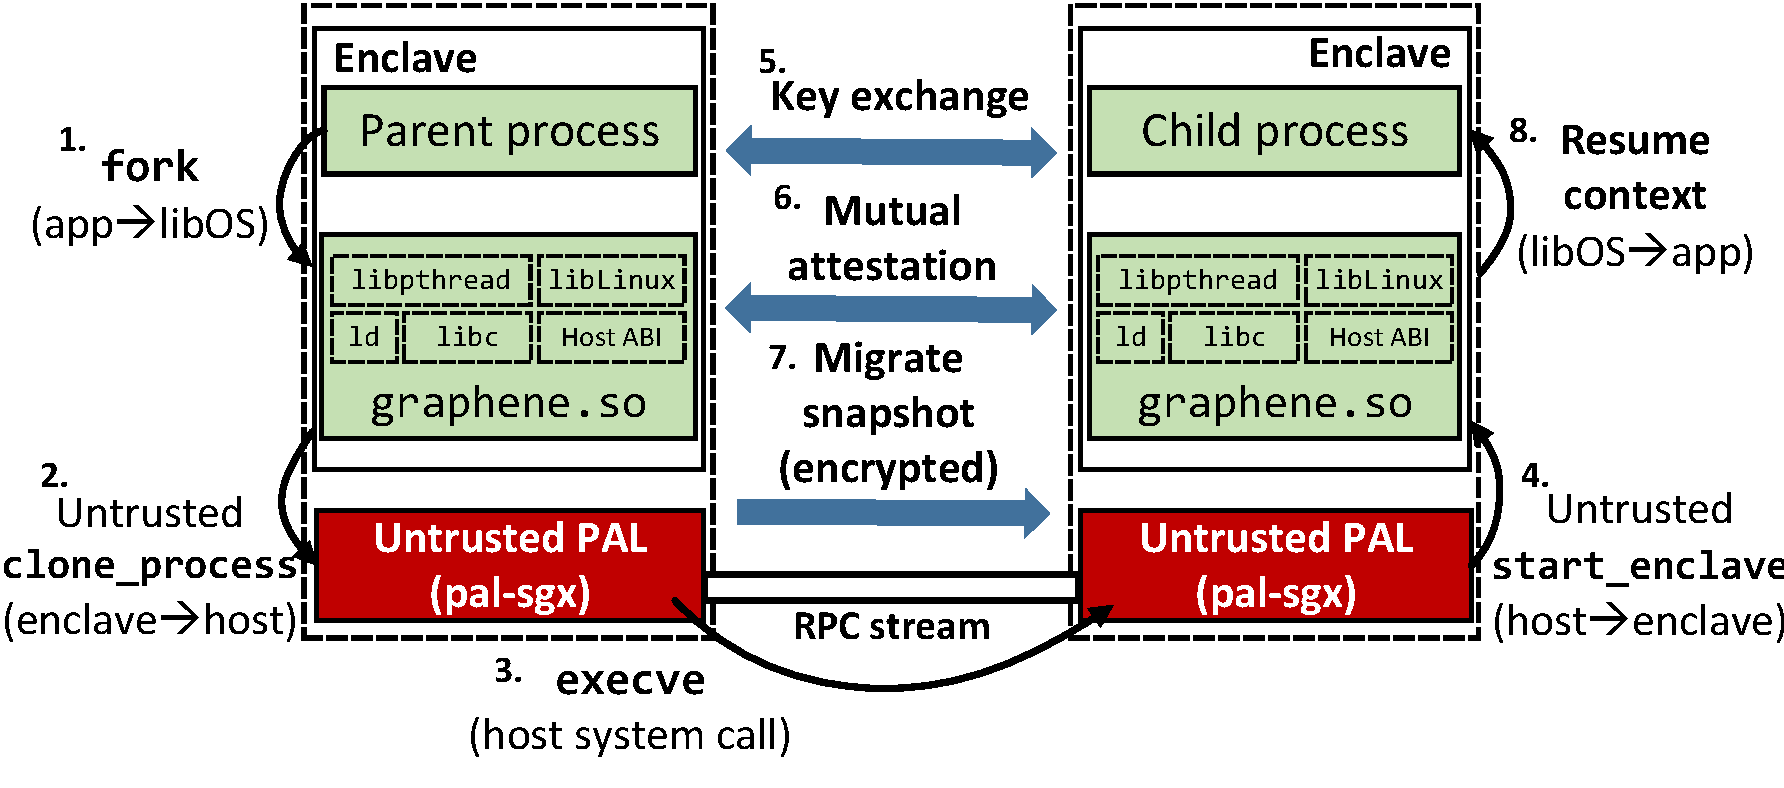
\includegraphics[width=6.5in]{graphene-sgx/figures/fork.pdf}
\footnotesize
\caption[Process creation in \graphenesgx{}]
{Process creation in \graphenesgx{}.
Numbers show the order of operations.
When a process forks, \graphenesgx{} calls {\tt execve} system call
on the untrusted host,
to create a clean enclave with the same \libos{} image.
Then the two enclaves build up the mutual trust by
exchanging a session key, verifying attestation of each other,
and migrating the process snapshot from the parent.}
\label{fig:graphene:sgx-fork}
\end{figure}

To securely create process across enclaves,
\graphenesgx{} builds trusted paths for enclaves to send process snapshots and coordinate shared states.
Since the enclaves do not directly share pages,
the coordination must be intermediated by the untrusted host.
The untrusted host may launch attacks on the multi-process abstractions of \graphenesgx{},
by either counterfeiting the behavior of either the forking or forked process,
or acting as man-in-the-middle between two processes.

%is capable of building up the trust to newly launched enclaves,
%through cooperation with an untrusted host.
%Once a clean and trusted new enclave is launched,
%The parent process will send a snapshot to the new one,
%to create a clone of itself.
%Snapshotting and migrating process states
%is a feature robustly implemented and heavily used in \graphene{} \libos{},
%of which we simply inherit the design.

When a isolated process forks,
\graphenesgx{} requests the untrusted host to create a clean enclave
of the forking process.
The parent and child process in their own enclaves
will coordinate over an encrypted RPC streams,
with the session key exchange at the beginning of coordination.
After securing the RPC streams,
the participating processes exchange attestation,
ensuring both sides are restricted to running the same application.
Once the mutual trust is built between the two processes,
further inter-process coordination is secured.
%because the parent and the child will be running the same binary,
%both enclaves can simply be expected to have the same measurement.
%To build up the trust, the two processes will open an encrypted channel
%using a session key,
%and exchange attestation generated by the processor.
%Once both sides have confirmed the integrity of the other,
%the parent process is safe to send its snapshot, encrypted, to the child
%through the said channel.
%The child process will restore the snapshot in its own enclave,
%making it a clone of its parent.
The design of process creation in \graphenesgx{} is shown as Figure~\ref{fig:graphene:sgx-fork}.

%Forking in \graphenesgx{} mainly defends against 3 types of attacks
%from the untrusted host:
%
%\begin{compactenum}
%
%\item The host pretends to be the child enclave, to expose the process snapshot
%sent from the parent.
%
%\item The host pretends to be the parent enclave, to compromise the
%child process using a malicious process snapshot.
%
%\item The untrusted host becomes a man-in-the-middle, which bounces
%encrypted messages between the child and parent enclaves, with session keys
%negotiated with both sides.
%
%\end{compactenum}
%
%As described earlier, attacks 1 and 2 are prevented by mutual attestation
%between the parent and the child,
%and encrypting the channel for sending the snapshot.
%The attestation signed by the processor proves that both entities communicating
%are valid \graphenesgx{} enclaves,
%and encrypting the channel prevents the snapshot being eavesdropped or
%counterfeited by the host.

To defend against the man-in-the-middle attack, we take advantage of
a user-customized 512-bit field
in the attestation structure generated and signed by the \sgx{} hardware.
This field is filled with a SHA-256 hash value of the agreed session key,
and the current enclave ID,
to prove that the attested party is the one who agrees on the key.

%Once a parent enclave forks a child, by default the child must be trusted
%to maintain its own security,
%because the migrated snapshot discloses all information in the parent.
%Unless the binary run in the parent enclave ensures
%that no secrets is stored in the enclave memory at the time of snapshotting,
%the parent enclave cannot simply drop the trust against the child.
%For example, a pre-forked Apache web server may want to keep each worker
%that responds to HTTP requests isolated,
%to avoid being compromised by one attacked worker.
%\graphene{} \libos{} provides an API for applications like Apache to explicitly
%specify isolation to untrusted child processes.
%\graphenesgx{} inherits the ability of dynamic process isolation,
%but developers are responsible for keeping confidential information
%from the untrusted children.

\paragraph{Implementing {\tt execve}.}
Unlike {\tt fork}, {\tt execve}
starts a process with a specified binary, often different from the callers,
in a clean process state.
%When a thread in the process, either single-threaded or multi-threaded,
%calls {\tt execve} in \graphenesgx{},
%\libos{} will migrate the calling thread to a new process,
%with clean process states except opened files cloned from the parent.
A key challenge for implementing {\tt execve} is to
identify trusted binaries that can be loaded into new enclaves as child processes.
Although a child process created by {\tt execve} does not start with
a snapshot of its parent,
The processes share states through inheriting file handles,
or future inter-process coordination.
The communication between the processes must be considered internal interaction of the application,
thus shall be protected from the host.

%Consider the case where the parent process and its child shares
%a multi-process abstraction (e.g., message queue).
%Even if only the parent side is provisioned by the client, the child side
%can still potentially compromise the secrets,
%by exploiting vulnerabilities in the shared abstraction.
%The trust between the parent and the child must be mutual,
%unless the two enclaves are strictly isolated.

As securing {\tt fork}, {\tt execve} is secured by the attestation of
the child processes' measurements.
\graphenesgx{} only allows a isolated process to create a child process
in an enclave whose measurement is listed in its manifest.
In addition, a child process does not verify the measurement of its parent,
but instead presents the measurements of all ancestors
to remote trusted server when attesting its own integrity.
In other word, for the same binary {\tt ls} isolated in the enclave,
the measurement reflects the distinction if the binary is called by,
say a shell or Apache server.

%To identify binaries that can be trusted (either as parents or children)
%during process creation,
%\graphenesgx{} requires each binary ported for an application,
%to be shipped with a list of binaries that can be {\tt execve}'d,
%and those that can be callers of {\tt execve} to the said binary.
%Each binary in the list is identified by its measurement, which is mutually attested
%between the parent and the child during process creation.
%This list must be signed by a private key provided by the client,
%while the public key must be included in the enclave measurement of the binary.

%\subsection{Securing Inter-Process Coordination}
%\label{sec:graphene:multiproc:ipc}
%
%After process creation, multiple processes in an application amy cooperate
%through sharing multi-process abstractions,
%such as signals or message queues.
%In \graphene{}, \picoprocs{} coordinate over RPC streams,
%to maintain the state of shared objects,
%as well as 
%the namespace states such as in which \picoprocs{} these objects are proxied.
%
%\graphene{} coordinates multi-process abstractions and namespaces
%by passing messages over RPC streams.
%Such a design is beneficial for supporting multi-process abstractions in enclaves.
%\graphenesgx{} inherits the same design of inter-process coordination,
%and the RPC streams used for coordination can be secured by the enclaves proactively on untrusted hosts.

%In \graphene{}, security isolation among multi-process abstractions,
%regardless of their semantics,
%are enforced by isolating the RPC streams used for coordination.
%Unfortunately, \graphenesgx{} cannot trust the host to faithfully isolate
%the RPC streams.
%Each enclave launched for an application must secure inter-process coordination
%spontaneously, by only communicating to enclaves that it has attested
%and exchanged secret keys with.
%Because inter-process coordination is completely transparent
%to the applications,
%all information sent over RPC streams must be encrypted,
%because \libos{} cannot determine whether the information may contain any secret.



%\section{Minimizing the TCB with the Non-Partitioned Model}

%\subsection{Reducing the TCB in \libos{}}
%\subsection{Partitioning the TCB in Multi-Process Applications}



\section{Implementation Details in \graphene{}}
\label{sec:graphene:impl}

\paragraph{Linux \pal{}.}
The majority of \pal{} calls are simple wrappers for similar Linux system calls, 
adding less than 100 LoC on average for translation between \pal{} and Linux abstractions.
The largest \pal{} calls are for exception handling, synchronization, and picoprocess
creation, which require multiple system calls and range from 500--800 LoC each.
Creating a new picoprocesses internally requires a {\tt vfork} and {\tt exec} of a clean 
application instance, and would be more efficiently implemented in the kernel.
Finally, the other major \pal{} components are an ELF loader (2 kLoC), headers (800 LoC),
and internal support code (2.3 kLoC).

\paragraph{Alternative \pal{} Ports.}
We prove the platform independence of \graphene{}
by porting \pal{} to \emph{FreeBSD}, \emph{OSX} and \emph{Windows}.
With the alternative host \pal{}, unmodified Linux binaries,
along with {\tt glibc} and {libLinux},
can be transparently run on the host.
For FreeBSD,
only 1.2 kLoC of the host \pal{} code need to be rewritten,
which are significantly less than FreeBSD Linux compatibility module (10.8 kLoC).
\pal{} components including ELF loader and internal support code can be shared by any \pal{} ports.

%\fix{We leave host \pal{} ports to non-unix OSes like Windows as future work,
%but previous works~\cite{porter11drawbridge,baumann13bascule} have already shown it feasible.}

\begin{table}[t!b!]
\footnotesize
\centering
\begin{tabular}{|l|rr|}
\hline
{\bf Component} & {\bf Lines} & ({\bf \% Changed})\\
\hline
GNU Library C ({\tt libc}, {\tt ld}, {\tt libdl}, {\tt libpthread}) & \libclines{} & $0.07\%$ \\
\hline
Linux Library OS ({\tt libLinux}) & 31,112 & \\
Linux host \pal{} & 11,644 & \\
Extra code for Linux \sgx{} host \pal{} & 9.354 & \\
% updated by Chia-Che on Oct. 10, 2013
\hline
%Storage Server & \fixmedp{XX} & \\
Reference monitor bootstrapper & \reflines{} & \\
Linux kernel reference monitor module ({\tt /dev/graphene}) & \sandboxmodlines{} & \\
Linux kernel IPC module ({\tt /dev/gipc}) & \gipclines{} & \\
\hline
\end{tabular}
\caption[Lines of code written or changed in \graphene{}]
{Lines of code written or changed to produce \graphene{}.  Applications and other libraries are unchanged.}
\label{tab:graphene:loc}
\end{table}


%% * most calls are a wrapper, \fixmedp{XX} LoC on average.
%% * Exception handling, sync, and process creation were harder (500-800 LoC each).  Process creation requires a clean instance (vfork+exec), would be simpler to implement in kernel.
%% * Other major components: ELF loader (2kLoC), headers(800 LoC), internal support code (2300 LoC)


%\fixmedp{Chia-Che, update LoC table}

\paragraph{Implementing Linux Personality.} 
%\fixmedp{Revisit the logical flow of these paragraphs}
The \graphene{} {\tt libLinux.so} implements a subset 
of the Linux system call API (currently \graphenesyscalls{} calls)
using only the \pal{} ABI to interact with the host.
We note that Linux exports a very long tail of infrequently used calls.
%applications.
A rough analysis of this tail indicates roughly 100 additional calls that can be implemented
with the existing \pal{} ABI and coordination framework, less than 10 administrative calls that will not make sense to expose to 
an application, such as loading a kernel module or rebooting the system, and roughly 54 that will require 
\pal{} extensions to meaningfully implement, such as controlling scheduling,
NUMA placement, I/O privilege, and shared memory.
In the last category of system calls, the degree to which actual host details should be exported versus emulated is debatable.

%We believe represent the most commonly used system calls.
%When an application requests a call or argument that {\tt libLinux.so} does not implement,
%the picoprocess exits with a distinct error message. 
Each time we have tested \graphene{} with a new application, the number of extra system calls
required has dropped---most recently we only added 4 calls
(namely, epoll\_create, epoll\_wait, semget and semop)
to support the Apache web server.
Thus, we believe \graphene{} implements a representative sample of Linux calls.

%such as {\tt sched\_setparam}, which manipulates scheduler-specific
%parameters or 
%{\tt uselib}, which has been abandoned 
%in {\tt glibc} version 2 in favor of a user-space dynamic linker.
%We do not plan to implement administrative interfaces, such as {\tt reboot}.
%The growth in the set of supported system calls has been driven by 
%the requirements of new applications we use to exercise \graphene{}, and has been 
%slowing considerably over time.

%directly to guests, and thus will not implement them in {\tt libLinux.so}.

% dp: :(
\begin{comment}
Most {\tt libLinux.so} code reimplements
Linux kernel functionality.  We found it expedient to 
read the Linux source in order to understand its behavior and then reimplement 
that behavior on the \pal{} ABI in most cases.
In some cases, such as the file caching code,
%directory entry (dentry) cache, 
we refactored code directly from the Linux kernel.
%% In these cases, we simplified data structures to only include data
%% we needed for a single application, and to hook in with other 
%% {\tt libLinux} subsystems.
%% An interesting direction for future work would identify techniques
%% to automatically import larger swaths of Linux kernel code, facilitating
%% adoption of new features and bugfixes.
\end{comment}

In order to use {\tt libLinux.so}, we modified \libclines{} lines of {\tt glibc} to replace 
system instructions with function calls into {\tt lib\-Linux.so},
and to cooperatively manage thread-local storage with {\tt libLinux.so} (Table~\ref{tab:graphene:loc}).

%All totaled, we only needed to modify \libclines{} lines of glibc source code to redirect all 
%system calls to {\tt libLinux} 

%\section{User-level {\tt fork} and other Linux library OS challenges}
%%% \vspace{5pt}
%%% \label{sec:fork}
%%% \noindent {\bf Copy-On-Write Fork.~}
%%% Creating a clean guest eases reasoning about security isolation, as all shared abstractions
%%% must be implemented using explicit data streams  between guests.
%%% This section describes how we implement these Unix abstractions in the guest
%%% %achieve a sensible division of labor between guest and host, and 
%%% without baking Unix personality into the host ABI.


\begin{comment}
\vspace{5pt}
\noindent{\bf Guest self-migration.~}  One of the key features of the host ABI
is that guest state can be programmatically read and recreated.
As a result, guests can checkpoint, migrate, and resume themselves in a new picoprocess,
potentially on a new host.  
Most of the library OS and application state are checkpointed simply 
by copying the contents of virtual memory into a file.
Checkpointing requires manually serializing a few key data structures
in {\tt libLinux} that are needed to resume the library OS from a checkpoint,
% interface directly with the PAL, 
including the thread states, handle table, and memory mappings.  

Resuming from a checkpoint involves restoring these key data
structures (handles, thread register contexts, memory mappings), and re-loading memory
contents from the checkpoint.  Most additional data structures
in {\tt libLinux}, and all application data structures,
are reloaded at the virtual address as before the checkpoint and work without modification.
\end{comment}

\begin{comment}
When a new guest begins execution, an input argument to {\tt libLinux} indicates
whether control should be transferred to the Linux loader ({\tt ld.so}) to start a new application instance, 
or whether a checkpoint should be loaded instead.
\end{comment}
%After the checkpoint is loaded, all threads resume execution on their stacks.

\paragraph{Implementing fork by (Ab)using Checkpoints.} 
Copy-on-write fork presented a particular challenge.
%when implemented using only a VM-like picoprocess abstraction.
As with a virtual machine, each new picoprocess 
is created in a ``clean'' state; fork is implemented in the \libos{}.
%yet applications require common Unix abstractions such as file handle inheritance and copy-on-write fork.

Graphene implements file Unix-style {\tt fork}
by leveraging portions of the checkpoint and migration code,
which can programmatically save and restore OS state (e.g., file handles, and memory mappings).
Rather than writing the checkpoint to a file, 
we developed an efficient bulk IPC mechanism to 
permit copy-on-write sharing of memory pages among processes.
Bulk IPC is a performance optimization over sending each byte of the parent address
space over a stream, although {\tt libLinux} can also implement {\tt fork}
over a stream.
Bulk IPC adds 3 calls to the host ABI,
and the host reference monitor only permits bulk IPC among
picoprocesses within a sandbox.

%% Conceptually, {\tt fork} could be implemented by checkpointing the parent,
%% modifying the primary thread's checkpoint 
%% so that the child returns 0 from the fork call 
%% (indicating it is the child),
%% and then immediately resuming the checkpoint in another picoprocess.

%% In practice, we optimize {\tt fork} performance by avoiding 
%% the use of an intermediate checkpoint file, instead transferring the checkpoint
%% directly to the child over a host-level bulk IPC
%%  mechanism (\S\ref{sec:linux:pal}).
%The Graphene bulk IPC abstraction adds 3 PAL calls 
%that allow guests to efficiently transfer large regions of memory to each other\fixmedp{after reordering, add a forward or back ref}.

Using our bulk IPC mechanism,
the sender (parent) can request that the host kernel copy
a series of pages, which need not be virtually contiguous,
into the receiver's address space.
The receiver (child) specifies where these pages should be mapped.
In both sender and receiver, the pages are marked copy-on-write.  
This bulk IPC mechanism sends pages out-of-band on a byte stream and guests also use the stream to send control messages 
indicating 
how many pages are being sent and how they should be interpreted.

Our IPC module is \gipclines{} lines of code (Table~\ref{tab:graphene:loc}), 
runs on multiple versions of Linux (2.6 and 3 series kernels), and
does not require
Linux kernel changes or recompilation.


\begin{comment}
A critical challenge in developing a Linux library OS was implementing 
handle inheritance in the guest.  In some cases, 
handles are easy to reproduce: an open file can simply be reopened in the child,
and the cursor offset adjusted (note that file handle offsets are a library abstraction
implemented over a memory mapped file).
Pipes, however, are not easily recreated without host support.
\end{comment}
%One option was to create explicitly named host-level byte streams,
%similar to System V or Windows named pipes.
%This strategy is simple to add to the Drawbridge host ABI and easy to program in {\tt libLinux},
%but complicates security isolation, as guests must be prevented from 
%opening a host-level pipe outside of their sandbox.

%A second option, which we pursue, is to only create anonymous bytes streams,
\paragraph{Inheriting File Handles.}
Graphene adds two PAL ABI functions that transfer 
stream handles out-of-band over reviously 
established byte streams within a sandbox.  Handle passing facilitates inheritance
and general-purpose RPC.
This mechanism is similar to Unix Domain Sockets,
which are commonly used by sandboxing systems. % such as plash~\citep{plash}.
This strategy allows a guest to seamlessly and explicitly 
share an open handle with another guest in the same sandbox, but prevents
a guest from sharing a handle with a guest outside of the sandbox.

\begin{comment}
\vspace{5pt}
\noindent{\bf Discussion.~}
A Graphene picoprocess can copy part or all its address space into a child
picoprocess relatively efficiently.
Although this mechanism is less efficient than an in-kernel {\tt fork},
we wanted to maintain the generality benefits of recent \liboses{},
and only added the minimal building blocks to the host ABI.
%we felt this design would bake Unix personality into the host kernel ABI,
%and  reintroduce security problems caused by accidental inheritance~\citep{close-on-exec}.
The transfer of data is explicit to the host, can be mediated by a reference monitor,
the sender, or the receiver.
For instance, recent Unix systems introduced a close-on-exec flag for file handles~\citep{close-on-exec}, 
which prevents inheritance of handles to sensitive files.  This can be implemented
either in a parent, by excluding the file handle from a checkpoint, 
or in the child, by closing this handle on an {\tt exec} call.
Our current implementation implements close-on-exec in the child for complete compatibility,
but a more security-sensitive application could easily implement ``close-on-fork'' semantics 
in the parent.
This clean division of labor retains full functionality
and facilitates extensibility.


\end{comment}


\begin{comment}
\vspace{5pt}
\noindent{\bf ABI Extensions.~}
\graphene{} extends the Drawbridge ABI with 9 additional \pal{} calls.
As discussed above, one creates a new sandbox, and 
5 additional calls were added for IPC.
We also add 3 calls to manage x86 segmentation registers
and exceptions (Bascule~\cite{baumann13bascule} adds
similar extensions).
\end{comment}

\paragraph{Synchronization.} Perhaps surprisingly, implementing Linux
synchronization appears substantially easier than Windows synchronization, 
as {\tt libLinux} did not require all of the various
synchronization ABIs provided by Drawbridge.
We believe the reason for this is that Linux has consolidated 
all user-level synchronization primitives to use futexes~\cite{franke02futex},
which are essentially kernel-level wait queues.
%In Windows parlance, this is simply an Event associated with a virtual address.
%Thus, our effort implementing synchronization was relatively straightforward.

%\papersection{\Thehostabi{}}
\label{sec:overview:host}

\issuedone{1.1.b}{Describe \thehostabi{} specification}
The development of \graphene{} starts with defining a simple host ABI (application binary interface) called \thehostabi{},
containing only OS abstractions essential to target applications.
%and is easily ported to different platforms.
%and minimal specifications for the host OSes and hardware.
%The host ABI is a new boundary between OSes (or hypervisors) and applications.
\Thehostabi{} separates
the implementation of an existing system API (application programming interfaces), which determines the compatibility against applications,
from hardware abstraction features, such as file systems, network stacks, and device drivers. 
\graphene{} moves the system API components
to a \libos{} in the userspace and reimplements the functionality using \thehostabi{}.
To port \graphene{} to a new host OS or hardware,
OS developers only have to implement \thehostabi{} on the target host system API,
%to new host OSes and hardware,
instead of paying a tremendous cost to translate the whole system API specification. Figure~\ref{fig:overview:porting} illustrates the porting process of \graphene{}.



%The host ABI separates the low-level, hardware management features, from the idiosyncrasy of system interface. 
%\graphene{} moves the upper layer of OS components,
%including the system calls and namespaces, into an library OS,
%leaving \thehostabi{} 
%as a narrowed interface to the host OSes and hardware.
%The host ABI intends to minimize the development effort on each host OS or hardware
%to mitigate the interface distinctions,
%to simply porting the OS abstractions defined in \thehostabi{}.


\begin{figure}[t!]
\centering
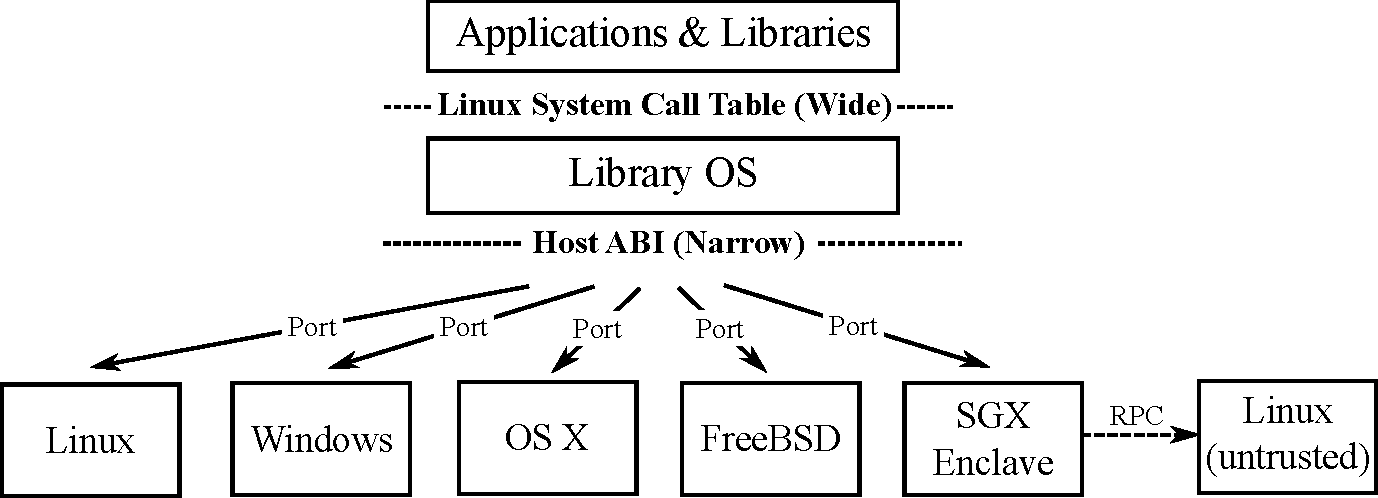
\includegraphics[width=30em]{porting.pdf}
\caption{Porting model of \graphene{}.}
%\vspace{-.1in}
\label{fig:overview:porting}
\end{figure}



\papersubsection{Platform Adaption Layers (PALs)}
\label{sec:overview:host:pal}


For each host OS or hardware, \graphene{} uses
a thin library called a {\bf platform translation layer (PAL)}
to translate among host interfaces.
%is loaded below the library OS, to translate each functions in \thehostabi{} to native system interfaces.
The main purpose of a PAL is to mitigate the semantic gap
between \thehostabi{} and
native host system APIs.
%The effort of PAL development is per host OS, whereas the library OS implementation is reusable on every hosts. %The simplicity of \thehostabi{} can be also estimated by the effort of implementing a PAL for each host.
By implementing a PAL on a new host OS or hardware,
users can reuse
the same \libos{} to run the same collection of unmodified Linux applications.
%To keep the porting effort low,
%the development of a PAL must be straightforward
%for average OS developers.
%to achieve with limited efforts.
%Based on the principle of porting simplicity, PAL development must be straightforward
%for average developers.







%The host ABI is defined for the simplicity of porting, as well as the sufficiency for implementing a library OS compatible to Linux.
%First of all, the number of host functions included in \thehostabi{}
%is much smaller than the number of system calls in a commodity OS such as Linux. 
\graphene{} currently contains PAL implementations for several popular OSes,
including Linux, \win{}, \osx{}, and FreeBSD.
%and \sgx{} with an untrusted Linux kernel.
Most of these OSes provide a POSIX-like system API similar to \thehostabi{}.
Due to the similarity, translating most of \thehostabi{} to one of the system APIs
are straightforward for average OS developers.
\Thehostabi{} is also much smaller than the actual POSIX API, making it extremely portable.



A part of \thehostabi{} may be challenging to port
on an OS,
due to unexpected system assumptions made by the OS.
For instance, \win{} does not support
fine-grained memory deallocation for de-privileged applications.
To implement system calls like \syscall{munmap} and \syscall{mprotect},
\graphene{} needs host ABIs to
deallocate or protect virtual memory pages at page granularity.
%A workaround is to change memory mappings at the physical page level,
%but will require running the \win{} PAL with root permissions.
%This type of porting challenges
%tends to be results of design decisions or assumptions made by OS developers.
%A \libos{} can potentially design
%different emulation strategies
%to compensate missing host abstractions.
A few host abstractions such as a bulk IPC feature are
optional to the host ABI;
if a host OS does not support these abstractions,
the \libos{} must fall back to alternatives. 

%In our experience, the development of a PAL is around ten thousand lines of code.

%For each port, the amount of code written for implementing \thehostabi{} is at the order of magnitude of thousands of lines of code, which is much more manageable than implementing a flat translation layer for system interfaces.


\begin{comment}
Based on the experience in \graphene{},
it is hard to ensure the portability of \thehostabi{} on every potential hosts.
%even a host ABI specialized for simplicity cannot guarantee to be portable on every hosts.
A host may simply lacks the functionality
for implementing a \hostapi{}.
The assumption is, maintaining the compatibility of \thehostabi{} poses a much less challenge than maintaining the whole system API.
Besides, the library OS may flexibly switch among emulation strategies
to compensate the absence of certain host abstraction.
As an example,
bulk IPC is optional in \thehostabi{} since its first definition,
due to the expectation
that implementing the feature may not be feasible on some hosts.
If bulk IPC is not available,
the library OS can fall back to RPC-based IPC, with a reasonable amount of performance penalty.
In the worst case, if there is no emulation strategies
to compensate for the absence of a \hostapi{},
user can predict the affected applications and avoid running these applications
on specific hosts. 
%at least users can predict whether an application will be affected and thus cannot run on certain hosts.
\end{comment}


%For a host OS that does not support ELF binaries, the PAL must follow the binary format which the host OS accepts, such as the Portable Executable (PE) format on \win{}.
%The PAL is the only layer in the user space which cannot be reused
%across different hosts. Besides the PAL, all of the other binaries in the user space are fully reusable, including the library OS, the supporting libraries, and the application executable.



%The host abstractions map to several common system calls in a commodity OS.
%For example, \funcname{StreamRead} and \funcname{StreamWrite} can directly map to the POSIX functions \funcname{pread} and \funcname{pwrite}, which are available in most OSes including Linux, BSD, \osx{}, and \win{}.
%More than half of the functions in \thehostabi{} can be counted toward this category.
%The rest of the host abstractions are either specific to Linux
%(e.g., TLS support),
%or belong to the POSIX functions that are not shared with commodity OSes
%(e.g., \funcname{mmap} on \win{}).
%The PAL emulates these host abstractions, using existing system interfaces available on the host OS, unless the software emulation is fundamentally impossible (e.g., restricted by the system interfaces), or too expensive (e.g., high overhead from copying data).



\papersubsection{Definitions and design principles}
 

\graphene{} defines \palcallnum{} calls in \thehostabi{} (also called \hostapis{}),
with a set of host abstractions
sufficient for \libos{} development.
%The host ABI defines the interaction between the library OS and a specific host.
%The \graphene{} library OS can be deployed on any ``host'' where \thehostabi{} has been ported.
This thesis defines
a {\bf host} of \thehostabi{}
to be an OS or hypervisor
which contains enough OS functionality for running a standalone application or virtual machine.
Most of the host targets in \graphene{}
are monolithic OSes,
including Linux, \win{}, \osx{}, and FreeBSD.
%which has defined a massive system API for programmability.
A monolithic OS 
usually contains a massive amount of system APIs,
which is sufficient for
implementing \thehostabi{}.


A special example of a host
is an \sgx{} (Software Guard Extensions) enclaves~\cite{intelsgx},
which
restricts OS functionality for security reasons.
The restrictions on \sgx{}
are results of a strong threat model
which distrusts any OS features except ones that are virtualized by the CPUs or migrated into enclaves.
The only way to obtain any missing OS features such as storage or networking
is to request through RPC (remote procedure call).
Requesting untrusted OS services through RPC also introduces new security threats that application developers tend not to anticipate~\cite{checkoway13iago,osdi16scone}.
Due to all the compatibility and security challenges discussed above,
this thesis uses \sgx{} as a representative example of a host
with unusual assumptions (e.g., threat models) and restrictions
compared to a monolithic OS.

%An innovative hardware abstraction like \sgx{} (software guard extensions)
%imposes unique assumptions and restrictions
%on a commodity OS,
%%creates a special host on top of Linux or \win{},
%%with unique interfaces and specifications regarding the host OSes.
%and thus creates a special host above the OS.

%If an OS has mutated or tweaked the interface for a hardware platform,
%such as an \sgx{} enclave 
%running on an untrusted Linux kernel,
%the combination of the OS (Linux) and the hardware platform (\sgx{}) is considered a specialized host.
%Especially, the \sgx{} port of \thehostabi{} faces several unique challenges,
%which will be discussed in Chapter~\ref{chap:sgx}.


\begin{comment}
%\fixme{each sentense should be a paragraph; starting the 2nd sentence}
\fixmedp{start with a strong opening stating the rationale}
The host ABI of \graphene{}
define functions needed from a host, in order to implement the library OS for reusing applications.
%to reuse an application and all its supporting libraries, including the \graphene{} library OS.
Each host of \graphene{} contains an OS and a hardware platform, either of which causes compatibility issues for running unmodified applications.
OS developers can port the library OS to a new host,
by simply reimplementing the narrowed host ABIs using abstractions available on the host.
%a new host platform.
%For each host which requires the compatibility for unmodified Linux applications, one only has to implement the narrowed host ABIs,
%instead of reimplementing the bloated, ``legacy'' system interfaces
%needed by the applications.
By implementing \thehostabi{}, OS developers skip the painful process of rebuilding the whole system interfaces of a commercial OS such as Linux.
The host ABIs strictly decouples the porting effort on the hosts from the compatibility feature for applications.
%The host ABIs decouple the OS development in the host and the implementation of compatibility for the existing Linux application.
What \thehostabi{} exposes is a simplified extended machine,
similar to a para-virtualization interface, capable of running the library OS as a lightweight virtual machine. % with compatibility against Linux applications.
%on which another layer of virtualization (i.e., the library OS) can be built to reproduce the compatibility for Linux.
\end{comment}


\begin{comment}
Two design principles drive the definition of \thehostabi{}s:
{\em simplicity} (i.e., easy to port on any hosts)
and {\em sufficiency} (i.e., containing enough OS functions for implementing a library OS).
The process of deciding \thehostabi{}s is comparable to
finding a ``pinch point'' within a OS implementation,
which can conveniently mediate a significant portion of OS execution paths for managing hardware abstractions.
%The two principles drive the development of \thehostabi{}s,
%The whole development of the \graphene{} library
%must be disciplined
%on extending \thehostabi{}s only when it is strongly required.
%of restraining extensions to \thehostabi{}s unless absolutely necessary.
The two principles
determine the soundness of the \graphene{} approach to improving compatibility
for any hosts.
\end{comment}


%%The host ABI is defined with partitioning in mind.
%\Thehostabi{} 
%determines a boundary which partitions several upper-level OS components, %, such as system calls and namespaces,
%into a library OS,
%%, as a dynamically-linked library which can be deployed
%%to various hosts.
%%The rationale behind the partitioning is based on the fact that not every OS component is equally important to compatibility, for applications which need to be ported across hosts.
%%When an OS is extended for a new hardware,
%%these OS components usually remain unchanged, or are predominantly reused.
%%Partitioning
%%into a library OS further guards these 
%in order to isolate the host idiosyncrasy. % on specific hardware. %any potential changes for adopting new hardware.
%%Similar isolation
%%exists in traditional OSes, but without partitioning:
%The strategy
%is also used in OSes:
%An example is the Linux virtual file system (VFS), an internal interface
%which encapsulates operations of file system drivers.
%%On the other hand,
%%drivers (e.g., drivers for file systems, block devices, or network cards)
%%and architecture-specific instructions
%%stay encapsulated in the host OS.
%%in the Linux kernels are usually encapsulated under a virtualized, in-kernel interface (e.g., the Linux virtual file system),
%%to simplify the development of the rest of the kernel.
%Similar to VFS,
%\thehostabi{} is intended
%to be a more ubiquitous interface,
%which encapsulates
%any host-specific behavior and semantic
%inside the host OS.
%%for encapsulating both OS and hardware idiosyncrasy on a wide range on hosts.
%%declares a ubiquitous system interface, to encapsulate both OS and hardware abstractions
%%for the library OS.




\Thehostabi{} shares several characteristics with a virtual hardware interface
exported by a hypervisor.
A generic, backward-compatible
virtual hardware interface
%a set of generic, virtual hardware,
%which the VM can control with the same drivers.
allows an unmodified OS kernel to run inside a virtual machine as on the bare metal.
%by exporting interfaces close to commodity hardware.
%To avoid additional porting effort, the virtual hardware are close to the typical commodity hardware.
%For instance, a virtual hardware interface
%usually includes a virtual NIC (network interface controller),
%such as the virtualized E1000 interfaces
%available in VMware workstation or QEMU.
%As a result, \thehostabi{} contains the
%typical OS features and interfaces, similar to the API of early UNIX systems.
The key difference between
a virtual hardware interface
and \thehostabi{}
is that \thehostabi{} does not target reusing a whole, unmodified OS kernel as a guest.
Instead, 
\thehostabi{} contains higher-level abstractions such as files and network sockets
to ensure portability on most host OSes.
The concept
of defining \thehostabi{}
with a customized guest OS (i.e., a \libos{}) running atop \thehostabi{} is similar to para-virtualization.
%\thehostabi{} expects the \libos{}
%to be rewritten and
%customized for \thehostabi{},
%similar to a 
%para-virtualizated VM.
%Compared to an actual para-virtualized VM,
A para-virtualized VM defines hypercalls as interfaces between a guest OS and a hypervisor.
Furthermore, \thehostabi{} avoids duplication of OS components
such as scheduler, page fault handler, file systems, and network stacks
between the host and \libos{}.
%Another difference is that \thehostabi{} is called by normal function calls, whereas para-virtualization relies on hypercalls.
To compare a VM and a \libos{} on a spectrum,
a VM reuses a whole OS on a wide, backward-compatible virtual hardware interface
whereas a \libos{} implements only system API components on a simplified host ABI.

The following paragraphs discuss the key design principles of \thehostabi{},
including porting simplicity, sufficiency for \libos{} development, and ease of migration.

\paragraph{Porting simplicity.}
%To reduce porting effort
%\thehostabi{}
%must be simple to port on a host OS or hardware.
To reduce porting efforts,
\graphene{} defines \thehostabi{}
using two strategies:
first, \graphene{} significantly reduces both the size and complexity of host OS features
that OS developers have to implement.
Effectively, \graphene{} avoids duplicated OS features and handling rare corner cases
on \thehostabi{}.
%The development of \graphene{} disciplinarily avoiding adding any functions to \thehostabi{},
%unless the library OS cannot internally implement an OS feature.
Second, the definition of \thehostabi{}
imitates common system APIs in a POSIX-like monolithic OS,
to directly translate most calls to
a few similar host abstractions.
%existing system calls or system library functions
%on each host.
%include functions which can be directly mapped to OS functions exported by the host.
%%the likelihood of finding similar features on the host, to be translated to functions in \thehostabi{}.
%The assumption that such a strategy is possible
%is based on
%the observation that
%%similarity of system interfaces is common among most OSes.
%similar OS functions, especially UNIX-style APIs,
%tend to commonly exist in most OSes.
%, to reduce the learning curve for programming applications.
For instance,
the stream APIs in \thehostabi{}, such as \palcall{StreamRead} and \palcall{StreamWrite}
are similar to
system calls like \syscall{read} and \syscall{write} exist on Linux, BSD, and POSIX API,
or \syscall{ReadFile} and \syscall{WriteFile}
on \win{}.
%with similar functionality and semantics.
%and 
%looks similar to \syscall{ReadFile} in \win{}, except the data types.
%The definition of \thehostabi{}
%is based on observations of the system interfaces in some of the important hosts,
%including Linux system calls and \win{} API.
%exported by the targeted hosts,
%and defines the functions in \thehostabi{}, to be easily translated to the native system interfaces.
%The host ABI is essentially a subset of the common features from every potential hosts.
%We expect %\thehostabi{} defined with simplicity in mind
%to be straightforward to port on most hosts,
%Most functions in \thehostabi{} can be easily translated to host system interfaces
%in various styles.
As the rest of this thesis proves, porting \thehostabi{} is straightforward
on most monolithic OSes.

%For example, \thehostabi{} defines \syscall{StreamRead} and \syscall{StreamWrite} for accessing I/O streams, similar to .
%xcept some nuanced details like order of parameters.


% by including OS functions , such as \syscall{FileRead} and \syscall{FileWrite}, similar to the Linux system calls, \syscall{pread} and \syscall{pwrite}.




\begin{comment}
The simplicity of \thehostabi{}s requires retaining a minimalist design of host functions. %, based on typical OS services for managing hardware.
%\graphene{} reduces the host functions
%to the bare minimum.
The host ABIs should only contain operations that
are absolutely necessary for requesting external hardware abstractions.
%A way to simplify \thehostabi{}s is to move host functions into the library OS
%and to replace them with wrappers consisting of other host functions.
Any functions that can be partially or wholly implemented inside the library OS
should be further simplified, or even removed from \thehostabi{}s.
%---in other words, whether \thehostabi{}s can be further reduced.
Moreover, \thehostabi{}s have to be simple enough to implement on
most hosts;
%In the simplest host ABIs, none of the host functions shall be able to internally implement the behavior of another host function,
%or the definition of \thehostabi{}s is further reducible.
that is, \thehostabi{}s should contain only OS functions that are commonly offered on
most hosts.
The host ABIs are close to simplified UNIX interfaces,
such as reading or writing a file or an I/O device as a byte stream,
or creating a virtual memory mapping.
%the most common OS functions
%offered on most of the potential hosts,
For most hosts,
implementing \thehostabi{} should be as straightforward as redirecting the functions to the closest host system calls.
%such as the Linux system calls or the \win{} APIs.
For example, the functionality of \syscall{StreamRead} and \syscall{StreamWrite} in \thehostabi{}s can loosely match with
\syscall{read} and \syscall{write} in Linux,
or \syscall{ReadFile} and \syscall{WriteFile} in \win{}.
%This thesis also evaluates the simplicity of \thehostabi{}s by counting the lines of code used to implement \thehostabi{}s on each host platforms.
Since most OSes have inherited a similar design from UNIX,
it is fair to assume finding
comparable OS functions %host platforms
to \thehostabi{} would be reasonably easy.
%fair to assume that \thehostabi{}s 
\end{comment}



\paragraph{Sufficiency for \libos{} development.}
%\Thehostabi{} defines
%the host abstraction available for a \libos{} to access host hardware abstractions.
To develop a \libos{} with compatibility against a wide range of applications,
\thehostabi{}
%are demonstrated by the fact that
%the exported host functions 
contain any OS abstractions that the \libos{} cannot easily emulate.
%and a full-function library OS is implemented on top of them.
For most hosts,
the host OS abstractions
%can be categorized into five types:
include
process creation, memory management, and I/O (typically, files and network connection)~\cite{dhamdhere2007os-textbook}.
%Besides security and protection,
%the definition of \thehostabi{} is closely related with hardware management,
%and offers the most basic abstractions for each category of OS functions.
%managing specific types of hardware,
%and each contain a few basic abstractions
%which can be expanded into other system interfaces.
%For example, the basic OS functions for memory management include
%allocating (\syscall{VirtMemAlloc}),
%protecting (\syscall{VirtMemProt}),
%and deallocating (\syscall{VirtMemFree}) memory regions. % at certain granularity
%(usually in pages).
%These basic functions can be used to implement other forms of memory allocation,
%such as growing heaps with \syscall{brk}
%or allocating thread-private stacks.
%The definition of the \drawbridge{} host ABI is a hint, for creating a list of host abstractions necessary for the library OS, including streams, memory, threads, and processes. 
%If \thehostabi{}s are insufficient for implementing certain system interfaces, one may extend \thehostabi{}s with the missing functions,
%with the discipline to retain the simplicity of \thehostabi{}s.
%The extension to \thehostabi{}s must be d, to keep the extension minimal, and to avoid adding redundant functions.
%The implementation of the \graphene{} library OS demonstrates that
%\thehostabi{} is sufficient for implementing significant portion of Linux system calls.
For each type of abstractions,
a monolithic OS may define several variants of system APIs with similar functionality.
For instance, Linux provides two system calls, \syscall{mmap} and \syscall{brk}, both for memory allocation in a process.
\syscall{mmap} allocates larger memory regions with page granularity,
whereas \syscall{brk} simply grows a single, continuous heap space for more fine-grained allocation.
Many applications such as GCC~\cite{gcc}
switch among system API variants in case one of them is unavailable on certain OS distributions.
This thesis shows that,
by adopting only the semantics of one of these similar APIs or abstractions, the host OS can stay simple with
the \libos{} emulating the rest of APIs.
For instance, \thehostabi{} includes \syscall{VirtMemAlloc}
as a similar feature as \syscall{mmap},
which is sufficient to emulating both \syscall{mmap} and \syscall{brk}.



\graphene{} defines \thehostabi{} partially based on
\drawbridge{},
a library OS for single-process \win{} applications.
The host ABI of \drawbridge{} 
contains 36 functions,
%demonstrates that its host ABI is sufficient
%for running a library OS in which 99.7\% of code comes from the \win{} 7 source.
%The host ABIs of \drawbridge{} are later extended
%for running a Linux-based library OS called Bascule~\cite{baumann13bascule}.
and several works have ported the host ABI to different hosts,
including \win{}, Linux, Barrelfish, and \sgx{}~\cite{porter11drawbridge,baumann14haven,mssql-on-linux,baumann13bascule}.
%and is capable of running a library OS for single-process, Linux applications, with a few host ABI changes~\cite{baumann13bascule}.
%ill loads and links the rest of application binaries, just like the native Linux loader (i.e., \code{ld.so}).
%\graphene{} takes the high-level definitions of the \drawbridge{} and Bascule host ABIs, and customizes for general-purpose Linux applications and a wider range of hosts. 
Although running \win{} and Linux applications may face
a different set of challenges,
the nature of their APIs is mostly similar, with a few exceptions.
During the development of \graphene{}, developers found the occasions in which
the host ABI of \drawbridge{}
is not sufficient to address Linux-specific challenges
and decide to extend \thehostabi{}.
Section~\ref{sec:overview:host:abi} and Chapter~\ref{chap:abi}
will further discuss the Linux-specific extensions of \thehostabi{}.


\paragraph{Migration.}
The \graphene{} library OS shares several features of VMs, including checkpointing and migrating a running application.
Migrating a process is also the key to emulating copy-on-write forking,
on a host without physical memory sharing (e.g., \sgx{}).
A hypervisor checkpoints and migrates a VM by snapshotting the VM states above a stateless virtual hardware interface. % as a clean boundary for snapshotting the application and OS state.
\Thehostabi{} is also defined to be statelessness,
by ensuring any states in the hosts to be temporary and reproducible to the applications and \libos{}.





\papersubsection{The \hostapis{}}
\label{sec:overview:host:abi}


%\fixmedp{the beginning doesn't capture the whole paragraph.}
%The host ABI shares several common abstractions with production OSes.
%The functions in \thehostabi{}
%define the basic features needed from the hosts, to run the library OS.
%The definition of the host functions
%should be unsurprising to average OS developers,
%making the implementation on a new host to be fairly straightforward.
%The host ABI reflects the common functionality of most OSes, including Linux and \win{}.
%Although the same OS abstractions may be defined
%as different idiosyncratic system interfaces on each host OSes,
%\graphene{} takes into consideration of porting the host functions to either OSes, in the most effortless way possible.





%fixmedp{give more of the background}
Table~\ref{tab:overview:abi} lists the \palcallnum{} calls defined in \thehostabi{}:
%Among these \hostapis{}, 
25 calls are inherited from the \drawbridge{} host ABI,
including functions to managing I/O (e.g., \palcall{StreamOpen}), memory allocation (e.g., \palcall{VirtMemAlloc}), scheduling (e.g., \palcall{ThreadCreate}), and several miscellaneous functions (e.g., \palcall{SystemTimeQuery}).
%Most of the host functions only affect the OS or hardware states
%related to the process itself.
%For example, \syscall{VirtMemAlloc} can only allocate memory in the calling process,
%and cannot affect other processes running in parallel.
%Only I/O streaming functions export states to the host OS, and share states with other processes or library OSes.
14 calls are added by \graphene{}, to implement Linux-specific features.
For example, unlike \win{} or \osx{}, Linux %The host ABI is also complemented with several Linux-specific abstractions, such as
delivers hardware exceptions to a process as signals.
Linux also requires 
the x86-specific segment registers (i.e., FS/GS registers)
to determine the location of thread-local storage (TLS), which can be hard-coded in application binaries by a compilation mode of GCC.
On \win{} or \osx{}, the x86-specific segment registers are mostly ignored, and even frequently reset to eliminate attack vectors.
%The host ABI contains host functions (), which can be directly called from the library OS. \graphene{} shows that \thehostabi{} is sufficient to implementing a large portion of the Linux system calls.
%These functions are not defined in \drawbridge{}, the \win{}-based library OS,
%because these abstractions do not exist in \win{}.
%The \drawbridge{} host ABI does not contain exception delivery because the feature is
%not commonly used in \win{} applications.
%Moreover, the x86 segment registers cannot be modified in \win{}
%because the OS assigns fixed values to these registers
%for the whole execution.
%Although \drawbridge{} excludes these abstractions, Bascule extends \thehostabi{} to include similar functions,
%demonstrating that the extension is indeed necessary.
\graphene{} discovers these abstractions as a necessity for implementing a rich Linux \libos{}.



\begin{table}[htp!]
\centering
\input{abi-table}
\caption{An overview of \thehostabi{} of \graphene{}. The ones marked with the symbol $\dagger$ are introduced in the initial publication of \graphene{}~\cite{tsai14graphene} or later extended for this thesis. The rest are inherited from \drawbridge{}~\cite{porter11drawbridge}.}
\label{tab:overview:abi}
\end{table}

%The interfaces, as part of \thehostabi{}, which access these host abstractions, are ultimately simplified to reduce the porting effort on each host.
%Unlike the system interfaces in the OS, \thehostabi{} does not prioritize backward compatibility. Therefore, \thehostabi{} includes only the minimum interfaces that the library OS needs to interact with the host. The host ABI does not have to include any of  the legacy system interfaces from a production OS, let alone preserving different flavors of system interfaces for backward compatibility.



\graphene{} introduces five calls for 
remote procedure call (RPC) between \libos{} instances
in a multi-process application.
\graphene{} simplifies porting multi-process abstractions
on each host OS
to implementing RPCs.
The basic RPC abstraction is 
a pipe-like RPC stream for message passing between processes.
To improve performance,
%RPC is critical for implementing the coordination of OS states
%across library OS instances.
%The basic form of RPC in \graphene{} is a pipe-like RPC byte stream, which a library OS can simply use to send messages.
%It is a common design choice
%to implement inter-process coordination through message-passing
%instead of shared memory, especially for hardware platforms that do not guarantee memory coherence~\cite{baumann09barrelfish}.
%A problem to the message-passing approach is the significant overheads
%on frequently exchanging distributed OS states.
\thehostabi{} defines an optional, bulk IPC abstraction
to send large chunks of virtual memory
across processes.
%The bulk IPC feature works similarly as sending the memory through RPC streams,
%but is much faster because it avoids copying memory in the host.


%for host platforms that urgently require lowering the RPC overheads.
%Another extension is for
%%\funcname{StreamSendHandle} and \funcname{StreamRecvHandle}
%delegating opened stream handles to another process, through a connecting pipe.
%The feature is similar to sending file descriptors
%through UNIX sockets in Linux, and is used to share opened network sockets with the \syscall{fork}'ed processes.
%%Another RPC abstraction is a bulk IPC channel; a process can use \funcname{PhsyicalMemoryCommit} to commit a large chunk of memory to a bulk IPC channel, which \funcname{PhsyicalMemoryMap} can map into another process, as copy-on-write. The library OS uses bulk IPC as an optimization to \syscall{fork}.
%Despite that either of the RPC primitives
%is not necessary easy to implement on every hosts, the inclusion of these host functions is completely optional, and the library OS can always fall back to the message-passing approach.



%All the host functions are designed to appear as ``stateless''
%as possible to the library OS.
%Being stateless to the library OS means that
%a host function does not preserve any permanent state of certain host abstraction.
%A stateless function can recover
%from disconnection of the library OS, and be reconnected at any timing.
%The host functions can maintain temporary bookkeeping for the convenience of porting,
%but should not assume the bookkeeping states to be permanent.
%The principle of defining all the host functions to be stateless
%is primarily for two purposes:
%{\em migration} and {\em security isolation}.
%For migration, the fact that the library OS can disconnect freely from the host functions simplifies the implementation of the migration feature.
%Migration is also an important foundation to implementing \syscall{fork}, because the cloned process need to receive a snapshot of the parent process.
%For security isolation, 
%a stateless host function is easier to check,
%because the security monitor only has to verify each instance of host function calls,
%instead of tracing multiple host functions over a longer period of time.

%the functions to access each host abstraction must appear \fixmedp{clarify `stateless'} stateless to the host, except for the handles to identify the resources. Each call to the host functions is independent. The arguments given for each call must be always be absolute values, instead of relative values.
%For example, the offset given to \funcname{StreamMap}, \funcname{StreamRead}, and \funcname{StreamWrite} (if the opened handle is a file) are offsets from the beginning of the file, and thus are irrelevant to how many bytes that are previously written or read.
%When enforcing isolation rules, the host OS can check the arguments of each calls to the host functions, independently and atomically.


%A host ABI (application binary interface) has to define the convention of application binaries, including the binary format and the linking procedure, as well as a set of  system interfaces.
%The host ABIs contain a minimal loader which recognizes a basic version of the ELF (Executable and Linkable Format), just enough to compose a binary of the library OS.
%The very initial loading procedure as part of \thehostabi{}s only loads a clean library OS instance.
%Each host of \graphene{} is supposed implement a minimal dynamic loader,
%which can load the \graphene{} library OS binary in ELF.
%The library OS then completes the dynamic loading procedure,
%by directly loading the Linux native dynamic loader (i.e., \code{ld.so}), and indirectly loading the rest of the application binaries.







\papersubsection{Host-enforced security isolation}
\label{sec:overview:host:security}


To target multi-tenant environments, 
\graphene{} enforces strong security isolation between mutually-untrusting applications running on the same host.
The security isolation of \graphene{} is comparable to running each application
in a VM or a container.
Just as a virtual hardware interface isolating each VM,
\thehostabi{} also enforces security isolation between library OS instances.
%according to the trust model of the applications.


On a trusted host OS,
\graphene{} delegates security isolation as a host-level feature.
The library OS and the application must mutually trust each other, due to lack of internal privilege separation in a process.
%The host ABI also separates API implementation
%from security isolation.
%To ensure isolation, each host must restrict access from the applications or the library OS, to any unauthorized host abstractions.
On each host, a reference monitor enforces security isolation policies, by access control on OS abstractions sharable among processes, including files, network sockets, and RPC streams.
%The host-level security isolation is orthogonal to API complexity.
Separating security isolation from API implementation simplifies security checks
for applications that only require
complete protection from other tenants.
%based on monitoring the references to host resources and rejecting authorized resource access.
%to the host abstractions.





%\graphene{} reduces the attack surface exposed to applications
%by restricting access to the host kernel ABI 
%and prevents access to unauthorized system calls, files, byte streams,
%and network addresses with a \emph{reference monitor}.
%The host kernel ABI exported by the \pal{} heavily 
%limits the ability of a \graphene{} application to interact with the rest of the system;
%any external interactions are further mediated by a reference monitor.
%Unlike a typical Linux system, \graphene{} applications cannot interact with shared 
%system daemons or other shared system resources.
%As a result, \graphene{} enforces security isolation similar to running applications in separate VMs---even
%applications that span multiple processes.


In \graphene{},
one or multiple processes of the same application run in a {\bf sandbox}.
Multiple library OS instances coordinate
in a sandbox
to present a unified OS view
to the application.
%As the library OS instances can coordinate shared OS states using simple RPC streams,
The design simplifies the enforcement of security isolation for multi-process abstractions.
\graphene{}
uses the reference monitor to block RPC streams across the sandbox boundary,
stopping applications in different sandboxes from accessing multi-process OS states.
%\graphene{} contributes a multi-process security model 
%based on the abstraction of a \emph{sandbox},
%or a set of mutually trusting processes.
%If a reference monitor exists, the reference monitor permits the processes within the same sandbox to communicate and exchange RPC messages, but disallows cross-sandbox communication.
The current design focuses on security isolation, although we do expect to extend the design for more sophisticated policies
in the future.

\begin{comment}
The only host abstractions that are shared across processes and must be mediated by the host for isolation are files, network sockets, and RPC streams
--- all other allowed host ABI modify only local process state, such as VMAs and threads.
%Thus, the reference monitor need only mediate file access, socket and RPC stream creation.
%an unprivileged daemon
%as well as extensions to the App\-Armor LSM~\cite{apparmor},
%which checks file and socket policies in the kernel.
%, reducing context switching overhead
%and the risk of race conditions~\cite{garfinkel03traps}.
In order for the reference monitor to restrict file access, socket and RPC stream creation,
each application includes a {\em manifest file}~\cite{hunt07rethink},
which describes a {\tt chroot}-like, restricted view of the local 
file system (similar to Plan 9's unioned file system views~\cite{pike90plan9}),
%including read-only shared files,
as well as {\em iptables}-style~\cite{iptablesman} network firewall rules.
To facilitate sharing read-only libraries, a manifest may specify a file system view which combines several different sub-directories of the local file system, and can prevent writing to files or directories.


For example, the \graphene{} reference monitor on the Linux host is implemented using \syscall{ioctl} to a special device (\code{/dev/graphene})~\fixme{a prospective design}.
A process is restricted by the Linux BPF-style system call filter, or the SECCOMP filter~\cite{seccomp}, to use \syscall{open} to access any files, or to \syscall{connect} or \syscall{bind} to any sockets.
It must use the \graphene{} special device to open or create streams, so the file paths or network addresses can be checked against the sandbox rules. The kernel module as the driver of the \graphene{} special device can coexist with any Linux Security Module (LSM), such as AppArmor~\cite{apparmor} or SELinux~\cite{selinux}.


When a new process is launched by the host, it begins execution in a new sandbox.  
Child processes may either inherit their parent's sandbox, or can be started in a separate sandbox---specified by a flag to the host abstractions of process creation.
A parent may specify a subset of its own file system view 
when creating a child, but may not request access to new regions of the host file system. 
%The restrictive policy enforced on the child will be written in a new manifest file generated by the parent, and the policy will be checked by the reference monitor.
The child may also issue an {\tt ioctl} call to 
dynamically detach from the parent's sandbox. The reference monitor prevents byte stream creation across sandboxes.
%among picoprocesses
%that are not in the same sandbox.
%and restricts external connections to remote URIs according to firewall rules in the manifest.
When a process detaches from a sandbox, effectively splitting the sandbox, the host must closes all RPC streams that could bridge the two sandboxes.
\end{comment}



\paragraph{Threat model.}
For most hosts, application trusts the host OSes as well a \libos{} instances in the same processes.
For multiple processes inside a sandbox,
the \liboses{} in these processes
also trust each other.
Applications or \liboses{} are not trusted by the host OSes or processes outside of the sandboxes.
Applications and \liboses{}
can become the adversary to the host OS,
by exploiting vulnerabilities on \thehostabi{}.
%the \graphene{} design reduces the attack surface between the hosts and the library OS instances, to defend against a malicious application.

%On a host with a reference monitor, the host OS and the reference monitor are both trusted, to mediate all system interfaces used to implement \thehostabi{}. The host must check all access to any abstractions with effects outside of a process's internal state, such as an opened file, or a connected network socket.
%Processes inside the same sandbox mutually trust each other. The adversary can run arbitrary code inside of one or more processes within one or more sandboxes.
%The adversary can control all code in its processes, including the library OS and the host-specific PAL.
%{\tt libLinux} and the \pal{}. 
%We also assume a trusted reference monitor process running on the host kernel that 
%launches \graphene{} applications and mediates all system calls with external effects,\fixmedp{define precisely}

%\graphene{} ensures that %The key security property the \graphene{} design upholds is that 
%the adversary cannot interfere with any victim picoprocesses
%in a separate sandbox.  
%The \graphene{} sandbox design ensures strict isolation: 
%if the only shared kernel abstractions are byte streams and files, 
%and the reference monitor ensures
%there is no writable intersection between sandboxes,
%the adversary cannot interfere with any victim picoprocess.


The threat model of \graphene{} on \sgx{}
contains the adversary from other hosts but excludes
the host OS, hypervisor, and any hardware except the CPU from its trusted computing base (TCB).
An untrusted OS or hypervisor
potentially has lots of opportunities to invade applications or VMs,
using Iago attacks~\cite{checkoway13iago}.
The challenges of porting \graphene{} to \sgx{} is not limited to resolving the compatibility issues of enclaves but also defending applications and \liboses{} against untrusted host OSes.







%%% The only processes allowed to run as standard kernel processes (non-\graphene{}) 
%%% are the reference monitor and
%%% system administration utilities that need more kernel interfaces than the \pal{} ABI provides.
%%% Ensuring that a collaborating picoprocess correctly implements
%%% some function (such as receiving a signal),
%%% as well as preventing exploitation of vulnerabilities in picoprocesses
%%% are beyond the scope of this work.

%\graphene{} reduces the system attack surface of the host, but does not change the size of its
%trusted computing base; however, reducing the effective system call table
%size of a picoprocess does facilitate adoption of a smaller host kernel,
%which we leave for future work.





%\paragraph{Linux Personality.}

%\paragraph{Memory and Binary Loading.}

%\paragraph{Exception handling.}

%\paragraph{Attestation.}

%\paragraph{Framework Support.}


\section{Evaluation of \graphene{}}
\label{sec:graphene:eval}

%\fixmedp{Missing back-of-the envelope for fork overheads, fraction of system calls using ipc}


This section evaluates \graphene{}'s multi-process coordination, security, cross-host migration, memory footprint, and performance.
We drive this evaluation with a selection of real-world applications that leverage multiple processes in \graphene{},
as well as with microbenchmarks and stress tests.
We organize the evaluation around the following questions:
\begin{compactenum}
\item How do \graphene{}'s startup and migration costs compare to running an application in a dedicated VM?
\item Given that RAM is often the limiting factor in VMs per system, how does \graphene{}'s memory footprint compare to other virtualization techniques?
\item What are the performance overheads of \graphene{} relative to a native Linux process or VM?
\item What additional overheads are added by the reference monitor?
\item How do \graphene{}'s overheads scale with the number of processes in a sandbox?
\item Does the \graphene{} reference monitor enforce security isolation comparable to running the application in a VM?  
\item What fraction of recent Linux vulnerabilities would \graphene{} prevent?
\end{compactenum}

%We note that no recent single-process library OSes are both publicly available
%and able to execute unmodified Linux binaries.

Except for scalability measurements, 
all measurements were collected on a 
Dell Optiplex 790 with 
a 4-core 3.40 GHz Intel Core i7 CPU,
4 GB RAM, and a 250GB, 7200 RPM ATA disk.
Our host system runs Ubuntu 12.04 server with host Linux kernel version 3.5, 
which includes KVM on 
QEMU version 1.0.
%Adding more detail of KVM environment
Each KVM Guest is deployed with 4 virtual CPU with EPT, 2GB RAM, a 30GB virtual disk image, Virtio enabled for network and disk, bridged connection with TAP, and runs the same Ubuntu and Linux kernel image.
We note that recent library OSes are either not openly available
or cannot execute unmodified Linux binaries.
Unless otherwise noted, \graphene{} measurements include the reference monitor.
%In order to assess the relative overhead of the monitor (\S\ref{sec:eval:micro}), 
%we include some microbenchmark measurements with and without the monitor.

%\paragraph{Seccomp filter optimization.~}
%Our benchmark shows that applying a seccomp filter can cause \fixme{xxx}\% overhead on {\tt getppid} syscall latency. We use a seccomp optimization patch, which just-in-time compiles filter code into machine code~\cite{seccomp-jit}.
%The result shows that the patch can improve xxx\% of {\tt getppid} latency.
%This patch is not officially adopted by Linux kernel, but it can be confirmed secure at least for x86-64 architecture.


\begin{table}[t!b!]
\footnotesize
\centering
\begin{tabular}{|l|r|rr|rr|rr|}
\hline
{\bf Test } & {\bf Linux } & \multicolumn{2}{c|}{{\bf KVM}}
& \multicolumn{2}{c|}{{\bf \graphene{}}} \\\hline

%Start-up time& 88.40& 3293296.77 & 3725349\% & 125350.73 & 1417\%& 622.00 & 604\% \\
Start-up   & 208 \us{} & 3.3 s & 15K\x{} & 641 \us{} & 3.1\x{}  \\
\hline
Checkpoint & N/A   & 0.987 s  &  &   416 \us{} &  \\
\hline
Resume     & N/A   & 1.146 s  &  &  1387 \us{} & \\
\hline\hline
Checkpoint size & N/A & \multicolumn{2}{l|}{105 MB} & \multicolumn{2}{l|}{376 KB}   \\
\hline
\end{tabular}
\caption[Startup, checkpoint, and resume times in Linux, KVM, and \graphene{}]
{Startup, checkpoint, and resume times for (1) a native Linux process,
(2) a KVM virtual machine,
(3) a \graphene{} \picoproc{},
(4) a \graphene{} \picoproc{} in a \sgx{} enclave,
 where appropriate. Lower is better.  
Overheads are relative to Linux.} 
\label{tab:graphene:startup}
\end{table}

\subsection{Process Migration and Application Startup}

%A key feature of VMs is the ability to move a running application to a new system.
\graphene{} supports migration of an application from a \picoproc{} on one machine
to a \picoproc{} on another machine by checkpointing the application,
copying the checkpoint over the network, and then resuming the checkpoint.
%We note that resuming a checkpoint executes entirely in userspace.
Table~\ref{tab:graphene:startup} shows the time to start
up a process, VM, or \picoproc{}; as well as the checkpoint and resume time for KVM and \graphene{}.
Migration across machines is a function of network bandwidth,
%% and checkpoint size, 
so we report checkpoint size instead. % of migration time.
%Only KVM and \graphene{} have the ability to checkpoint and resume, and are the only data points listed.


\graphene{} shows dramatically faster initialization times than a VM. This is not surprising,
since \graphene{} is substantially smaller than an OS kernel. 
Similarly, checkpointing and restoring a 4 MB application on \graphene{} is 1--4 times faster than checkpointing or restoring a KVM guest.



%\fixmedp{Error bars on mem usage graphs missing}

\subsection{Memory Footprint}
\label{sec:graphene:eval:mem}

We begin by measuring the minimal memory footprint of a simple ``hello world'' program 
on Linux (352 KB) and \graphene{} (1.4 MB).
Thus, one would expect roughly 1 MB of extra memory usage for any single-\picoproc{} application.
Because of copy-on-write sharing, however, the incremental cost of adding additional ``hello world'' children
is only about 790 KB per process.
%, although this will vary based on usage.

%Figure~\ref{fig:graphene:memusage} lists memory overheads of 
%a diverse set of {\em unmodified}
%applications, including 
%a {\tt make -j 4} of Gra\-phene's {\tt libLinux}
%using the {\tt \gcc{}} compiler (v4.4.5), 
%%\busy, a software which combines tiny versions of most common UNIX utilities into a single
%%small executable;
%the \light{} web server (v1.4.30) with 4 threads,
%the Apache web server (v2.4.3) with 4 processes,
%and the \busy{} shell (v4.1) executing the shell script test ({\tt multi.sh}) from the Unixbench suite (v5.1.3)~\cite{unixbench}.
%We measure memory utilization based on the maximum kernel-reported resident set size
%of each process or VM. For most applications, memory usage was fairly constant across inputs,
%so we only display representative examples.
%
%\begin{figure}[t!]
%\centering
%\includeplot[0.5]{apps-memusage}
%\centerline{\includegraphics[width=\linewidth]{figures/memusage.pdf}}
%\caption{Memory usage of applications on Linux, \graphene{}, and KVM, in MB.  Lower s better.
%\label{fig:graphene:memusage}}
%\end{figure}


We found that the memory footprints of compilation were a function of the 
size of the source base, even on Linux; we select compile of {\tt libLinux} as a representative example.
\graphene{} adds less than 15\% overhead in all cases.
%every compilation we measured on \graphene{} had less than 10\% memory overhead.

Unixbench on \graphene{} uses substantially more memory at a given time than native Linux---more than double.
In these samples, however, \graphene{} also had 3--4\x{} as many processes
running; this is because Unixbench simply spawns all of the tasks in the background, rather than
executing them sequentially.   Because \graphene{} processes execute more slowly (attributable to a slower {\tt fork}---\S\ref{sec:graphene:eval:perf}),
a given sample will include more \picoprocs{}, pushing total memory usage higher.
Thus, we expect that further tuning {\tt fork} performance will lower sampled memory usage.


Across all workloads, \graphene{}'s memory footprint is 3--20\x{}  
smaller than KVM.  
For all tests, we used a minimal KVM disk image, 
%formatted as a 30GB\fixmewkj{this can be changed to be smaller, but I don't know if disk size would impact memory} raw disk image with ext4. The root image was 
generated using debootstrap 1.0.39ubuntu0.3 and supplemented only by packages required to obtain, compile, and run the experiments.
In order to make memory footprint measurements as fair as possible to KVM, 
we used both the virtio balloon driver and kernel same page merging (KSM)~\cite{ksm}.
We also reduced the RAM allocated to the VM to the smallest size without harming performance---128MB.  We note that memory measured includes memory used by QEMU for VM device emulation, 
adding a few dozen MB.
%hence the total is 
%a few dozen MB higher than the RAM allocated to the VM.

If the smallest usable Linux VM consumes about 150 MB of RAM, our measurements indicate that 
one could run anywhere from 12--188 libOSes within the same footprint.


\begin{table}[t!b!]
\footnotesize
%\tiny
\centering

\begin{tabular}{|l|rr|rrr|rrr|rrr|}
\hline
&\multicolumn{11}{c|}{Execution time (s), +/- Conf. Interval, \% Overhead} \\
\hline
{\bf \gcc/make} & \multicolumn{2}{c|}{\bf Linux} & \multicolumn{3}{c|}{{\bf in KVM}} & \multicolumn{3}{c|}{{\bf \graphene{} + SC + RM}} & \multicolumn{3}{c|}{{\bf \graphene{} + \sgx{}}} \\
\hline
% gcc
%\multicolumn{2}{|l|}{helloworld} & .02 & .02 & 0 \% & .03 & 100 \% \\ 
%\hline
%oggenc & 1.42 & .01 & 1.51 & .00 & 6 \% & 1.43 & .00 & 1 \% \\\hline
gcc (helloworld)  & 0.020 & .000 &  0.022 & .000 & 7 \% &  0.023 & .000 &  12 \% & 6.097 & .012 & 298 $\times$  \\\hline
gcc (.7M\loc{})   & 21.64 &  .00 &  23.37 &  .02 & 8 \% &  21.88 &  .00 &   1 \% & 75.41 & .03 & 248 \%  \\\hline
make bzip2        & 2.332 & .000 &  2.448 & .000 & 5 \% &  2.407 & .000 &   3 \% & \multicolumn{3}{c|}{not supported yet}   \\\hline
make -j4 bzip2    & 0.888 & .000 &  0.967 & .000 & 9 \% &  0.923 & .004 &   4 \% & \multicolumn{3}{c|}{not supported yet}   \\\hline
make libLinux     & 4.832 & .000 &  5.037 & .000 & 4 \% &  5.112 & .001 &   6 \% & \multicolumn{3}{c|}{not supported yet}   \\\hline
make -j4 libLinux & 1.361 & .000 &  1.413 & .000 & 4 \% &  1.459 & .000 &   7 \% & \multicolumn{3}{c|}{not supported yet}   \\\hline



\hline\hline
Ap. Bnch     & \multicolumn{11}{c|}{Avg Throughput (MB/s), +/- Conf. Interval, \% Overhead} \\
\hline
{\bf Apache} & \multicolumn{2}{c|}{\bf Linux} & \multicolumn{3}{c|}{{\bf in in KVM}} & \multicolumn{3}{c|}{{\bf \graphene{} + SC + RM}}  & \multicolumn{3}{c|}{{\bf \graphene{} + \sgx{}}} \\
\hline
25 conc     & 6.282 & .005 & 5.327 & .031 & 18 \% & 4.586 & .002 & 36 \% & 2.312 & .192 & 171 \%    \\\hline
50 conc     & 6.305 & .002 & 5.420 & .060 & 16 \% & 4.555 & .012 & 38 \% & 2.752 & .463 & 129 \%  \\\hline
100 conc    & 6.347 & .010 & 5.152 & .036 & 22 \% & 4.572 & .009 & 39 \% & 2.488 & .781 & 155 \%   \\\hline

{\bf \light{}} & \multicolumn{2}{c|}{\bf Linux} & \multicolumn{3}{c|}{{\bf in KVM}} & \multicolumn{3}{c|}{{\bf \graphene{} + SC + RM}} & \multicolumn{3}{c|}{{\bf \graphene{} + \sgx{}}} \\
\hline

25 conc    & 6.66 &.01 &6.46 &.03 &3 \% &5.65 &.00 &18 \% & 2.124 & .072 & 171 \%    \\\hline
50 conc    & 6.65 &.13 &6.41 &.02 &4 \% &4.79 &.00 &39 \% & 2.437 & .107 & 171 \%    \\\hline
100 conc   & 6.69 &.01 &6.39 &.03 &5 \% &4.56 &.01 &47 \% & 2.417 & .235 & 171 \%    \\\hline

\hline\hline
%%%%% UnixBench

  & \multicolumn{11}{c|}{Execution Time (s), +/- Conf. Interval, \% Overhead} \\
\hline
{\bf bash } & \multicolumn{2}{c|}{\bf Linux} & \multicolumn{3}{c|}{{\bf in KVM}} & \multicolumn{3}{c|}{{\bf \graphene{} + RM}} & \multicolumn{3}{c|}{{\bf \graphenesgx{}}} \\
\hline
%2.1 s linux
%graphene 10.06s

%bash
Unix utils & 0.87 & .00 & 1.10 & .01 & 26 \% & 2.01 & .00 & 134 \% & \multicolumn{3}{c|}{not supported yet} \\\hline
Unixbench  & 0.55 & .00 & 0.55 & .00 &  0 \% & 1.49 & .00 & 192 \% & \multicolumn{3}{c|}{not supported yet} \\\hline
\end{tabular}
\caption[Application benchmark results in Linux, KVM and \graphene{}]
{Application benchmark execution times in a (1) native Linux process, (2) a process inside a KVM virtual machine, (3) a \graphene{} \picoproc{} with the SECCOMP filter ({\bf +SC}) and reference monitor ({\bf +RM}), and (3) \graphene{} in \sgx{} enclaves. }
\label{tab:graphene:apps}
\end{table}


\subsection{Application performance}
\label{sec:graphene:eval:perf}

Table~\ref{tab:graphene:apps} lists 
execution time of our {\em unmodified} 
application benchmarks (detailed in \S\ref{sec:graphene:eval:mem}).
All applications create multiple processes,
except for \light{}, which only creates multiple threads.
Each data point is the average of at least six runs, 
and 95\% confidence intervals are listed in the table.

We exercise  {\tt \gcc{}}/{\tt make}
with inputs of varying sizes:
%the pbzip2 compression utility (v1.1.6, 4 KLoC),
%the ogg sound encoder (v1.0.1, 5 KLoC),
%GNU {\tt make} (v3.82, \fixmedp{XX} KLoC)
bzip2 (v1.0.6, 5KLoC, 13 files),
\graphene{}'s {\tt libLinux} (31 KLoC, 78 files)
and \gcc{} (v3.5.0, 551 KLoC, collected as a single source file). 
We benchmark Apache (4 preforked workers) and \light{} (4 threads) with 
\ab{},
which issues 25, 50, and 100 concurrent requests
to download a 100 byte file 50,000 times.

We exercised \busy{} with 
300 iterations of the Unixbench benchmark~\cite{unixbench}, as well as 
300 iterations of a simple shell script benchmark that runs 6 common shell script commands
({\tt cp}, {\tt rm}, {\tt ls}, {\tt cat}, {\tt date}, and {\tt echo}).

Compilation workloads incur overheads ranging from 5--30\%.
%All compilation workloads have minimal overheads compared to native when executed sequentially;
Parallel compilation on both \graphene{} and Linux yields comparable  speedups  over sequential,
but the percent overhead increases for parallel \graphene{}.
For instance, {\tt make -j4 libLinux} speeds up 3.7\x{} on Linux and 3.4$\times$ on \graphene{}.
The compilation overheads are primarily from the reference monitor---nearly all for bzip2 and gcc, and half for {\tt libLinux}.
%Nearly all of the overhead from the bzip2 and gcc compilations are from the reference monitor; about half of the overheads of {\tt libLinux} compile 
%are the reference monitor and half are \graphene{} itself.
In the case of both \busy{} workloads, the key bottleneck is the {\tt fork} system call.
Profiling indicates that half of the time in {\tt libLinux} is spent on {\tt fork} in both benchmarks.
The trend is exacerbated in Unixbench, which creates all of the processes at the beginning and
waits for them all to complete; because \graphene{} cannot create children as quickly as native, this leads to 
load imbalance throughout the rest of the benchmark.  

With the reference monitor disabled,  \light{} has equivalent throughput to a native Linux process;
as discussed in the next subsection, these overheads come from checking paths in the monitor.
The Apache web server loses about half of its throughput relative to \light{} on \graphene{}.
The primary bottleneck in Apache relative to \light{} is System V semaphores,
%, which account for about 
%one third of the additional time spent in {\tt libLinux}
%relative to \light{}, 
and the remaining overheads are attributable to more time spent waiting for input.
The overheads for both \light{} and Apache on KVM are primarily attributable
to bridged networking.





\subsection{Micro-benchmarks}
\label{sec:graphene:eval:micro}

In order to understand the overheads of individual system calls,
Table~\ref{tab:graphene:lmbench} lists 
a representative sample of 
tests from the
\lmbench{} suite, version 2.5~\cite{McVoy:lmbench}.
Each row reports a mean and 95\% confidence interval;
we use the default number of iterations for each test case.
%We have added code to \lmbench{} to also calculate 95\% confidence intervals 
%within a run~\footnote{The lmbench authors deliberately exclude variation statistics
%because most methods assume a known distribution, generally a normal distribution---an 
%assumption which is often not the case for a computer microbenchmark~\cite{staelin05lmbench}.
%Though confidence intervals should be taken with a grain of salt, 
%we include them because they clearly indicate that these experiments have very low variance. In 
%a few cases of minor performance improvement, one can assess the impact of noise.}.
To measure the marginal cost of the reference monitor, we report numbers with and without 
the reference monitor.

%The performance of \graphene{} relative to Linux varies
%based on the system call.  
In general, calls that can be serviced inside the library are faster than native,
whereas calls that require translation to a native call incur overheads typically under 100\%.
For instance, 
the self-signaling test (sig overhead)
just calls the signal handler as a function,
which is almost twice as fast
as the Linux kernel implementation.  

\begin{table}[t!b!]
\footnotesize
\centering
\begin{tabular}{|l|rr|rrr|rrr|rrr|}
\hline
{\bf Test } & \multicolumn{2}{c|}{{\bf Linux}} & \multicolumn{3}{c|}{{\bf \graphene{}
}} & \multicolumn{3}{c|}{{\bf \graphene{} + SC + RM}} & \multicolumn{3}{c|}{{\bf \graphene{} + \sgx{}}} \\
&
\usec{} & +/- & 
\usec{} & +/- & \%O &
\usec{} & +/- & \%O & 
\usec{} & +/- & \%O \\

\hline

syscall        &  0.045 & .000 &  0.014 & .000 & -68.9 &    0.014 & .000 & -68.9 &  0.014 & .000 &   -68.9 \\\hline
read           &  0.115 & .000 &  0.118 & .000 &   2.6 &    0.118 & .000 &   2.6 &  0.119 & .000 &     3.5 \\\hline
write          &  0.115 & .000 &  0.115 & .000 &   0.0 &    0.115 & .000 &   0.0 &  0.115 & .000 &     0.0 \\\hline
stat           &  0.332 & .000 &  1.154 & .000 & 247.6 &    1.161 & .000 & 249.7 &  1.167 & .000 &   251.2 \\\hline
fstat          &  0.107 & .000 &  0.189 & .000 &  76.6 &    0.189 & .003 &  76.6 &  0.189 & .000 &    76.6 \\\hline
open/close     &  0.880 & .003 &  2.552 & .005 & 190.0 &    2.816 & .002 & 330.0 & 17.189 & .031 & 1,853.3 \\\hline
select file    &  3.360 & .001 & 11.536 & .003 & 243.3 &   11.647 & .004 & 246.6 & 11.567 & .003 &   244.3 \\\hline
select tcp     & 10.590 & .002 & 11.679 & .002 &  10.3 &   12.050 & .000 &  13.8 & 14.594 & .239 &    37.8 \\\hline
sig install    &  0.126 & .000 &  0.126 & .000 &   0.0 &    0.126 & .000 &   0.0 &  0.122 & .000 &    -3.2 \\\hline
sigusr1        &  0.951 & .000 &  0.184 & .000 & -80.7 &    0.188 & .000 & -80.2 &  0.184 & .000 &   -80.6 \\\hline
sigsegv        &  0.263 & .000 &  1.467 & .000 & 457.8 &    1.681 & .000 & 539.2 &  \multicolumn{3}{c|}{not supported yet}  \\\hline\hline
TCP            &  8.354 & .001 &  9.121 & .002 &   1.8 &    9.699 & .002 &  16.1 & 15.921 & .002 &  91 
\\\hline
UDP            &  7.222 & .002 &  9.450 & .002 &  30.8 &    9.995 & .001 &  38.4 & 15.671 & .003 & 116 
\\\hline
AF\_UNIX       &  4.937 & .011 &  5.024 & .001 &   1.8 &    6.155 & .010 &  24.7 & 12.567 & .003 & 152 
\\\hline\hline
fork+exit      &  66.86 & 0.09 &   380.47 & 3.55 & 469 &   442.83 & 1.39 &   562 & 1.22 \asec{} & .11 & 18k $\times$ \\\hline
fork+fork+exit & 148.32 & 0.55 &   778.00 & 6.87 & 424 &   915.67 & 3.35 &   517 & 2.66 \asec{} & .11 & 18k $\times$ \\\hline
vfork+exec     & 141.53 & 0.18 &   487.67 & 5.05 & 245 &   547.30 & 5.22 &   286 & 1.11 \asec{} & .06 &  8k $\times$ \\\hline
fork+exec      & 194.93 & 0.20 &   810.00 & 3.27 & 315 &   878.50 & 1.89 &   350 & 2.94 \asec{} & .21 & 15k $\times$ \\\hline
fork+fork+exec & 266.89 & 0.36 & 1,200.60 & 5.20 & 349 & 1,387.75 & 6.21 &   420 & 3.98 \asec{} & .50 & 15k $\times$ \\\hline
fork+sh        & 499.64 & 0.67 & 1,726.75 & 6.14 & 245 & 1,912.00 & 3.83 &   283 & \multicolumn{3}{c|}{not supported yet} \\\hline
%\hline
%UDP lat.&7.26&0.0&10.35&0.1&43&11.63&0.1&60 \\\hline
%TCP lat.&8.70&0.0&9.84&0.1&13&11.48&0.1&32 \\\hline
%\hline
%%%  \bf{Test} & K/s & +/- & K/s & +/- & \%O & K/s & +/- & \%O \\\hline
%%% %% \bf{Test} & \bf{K/s} & \bf{+/-} & \bf{K/s} & \bf{+/-} & \bf{\%O} & \bf{K/s} & \bf{+/-} & \bf{\%O} \\\hline
%%% 0K creat & 174 & 0.9 & 72 & 0.1 & 143 & 77 & 0.2 & 125 \\\hline
%%% 0K del & 232 & 1.2 & 130 & 0.5 & 79 & 117 & 0.2 & 98 \\\hline
%%% 4K creat & 120 & 0.1  & 33 & 0.0 & 265 & 31 & 0.0 & 284 \\\hline
%%% 4K del & 184 & 1.3  & 112 & 0.1 & 64 & 104 & 0.2 & 78 \\\hline
%%% 10K creat & 83 & 0.1  & 28 & 0.0 & 195 & 27 & 0.0 & 204 \\\hline
%%% 10K del & 149 & 0.3  & 94 & 0.1 & 58 & 88 & 0.2 & 69 \\\hline
\end{tabular}
\caption[\lmbench{} benchmarking results in Linux, KVM and \graphene{}]
{\lmbench{} comparison among (1) native Linux processes, (2) \graphene{} \picoprocs{} on Linux host, both without and with the SECCOMP filter ({\bf +SC}) and reference monitor ({\bf +RM}), and (3) \graphene{} in \sgx{} enclaves.
Execution time is in microseconds, and lower is better. 
%The file system is measured in thousands operations per second, and higher is better.
Overheads are relative to Linux; negative overheads indicate improved performance.} 
\label{tab:graphene:lmbench}
\end{table}


The most expensive system calls occur when {\tt libLinux} inadvertently duplicates work
with the host kernel.  
For instance, many of the file path and handle management calls duplicate some of the effort of the host file system,
leading to a 1--3\x{} slower implementation than native.
As the worst example,
{\tt fork+exit} is 5.9\x{} slower than Linux.
Profiling indicates that about one sixth of this overhead is in process creation, which 
takes additional work to create a clean \picoproc{} on Linux; we expect this overhead could be reduced
with a kernel-level implementation of the process creation ABI, rather than emulating this behavior on {\tt clone}.
Another half of the overhead comes from the
{\tt libLinux} checkpointing code (commensurate with the data in Table~\ref{tab:graphene:lmbench}), which 
includes a substantial amount of serialization effort which might be reduced by checkpointing the data structures in place.
A more competitive {\tt fork} will require host support and additional {\tt libLinux} tuning.
%Thus, we think a competitive {\tt fork} implementation will require both a more suitable host kernel
%and more tuning in the {\tt libLinux} code. 
%\fixmewkj{explain why TCP faster than UDP?}

We also measure the overhead of isolating a \graphene{} \picoproc{} inside the reference monitor.
Because most filtering rules can be statically loaded into the kernel,
the cost of filtering is negligible with few exceptions.
%TCP and UDP latency is increased slightly because the monitor checks
%the arguments of the {\tt connect} system call.
Only calls that
involve path traversals, such as {\tt open} and {\tt exec}, result in substantial overheads relative to \graphene{}.
%%, adding an additional 100--200\% overhead. This is 
%because the AppArmor extensions must verify that
%the requested paths are in the permitted file system view.
%Alternative implementations, such as a {\tt chroot-ed} environment using the aufs unioning file system version 3.0~\cite{aufs},
%resulted in opens that were {\em twice} as slow as our LSM extensions.
An efficient implementation of an environment similar to FreeBSD  jails~\cite{jails}
would make all reference monitoring overheads negligible.

\begin{table}[t!b!]
\footnotesize
\centering
\begin{tabular}{|ll|rr|rrr|}
\hline
\multicolumn{2}{|c|}{{\bf Test}} &
\multicolumn{2}{c|}{{\bf Linux}} &
\multicolumn{3}{c|}{{\bf \graphene{}}} \\
 & & \us{} & +/- & \us{} & +/- & \\
\hline
msgget   & in-process    & 3320	& 0.7 &  2823 & 0.3 &	-15	\%		\\
(create) & inter-process & 3336	& 0.5 &  2879 & 3.6 &	-14	\%		\\
         & persistent    &  N/A	&     & 10015 & 0.7 &	202	\%      \\
\hline								
msgget   & in-process    & 3245	& 0.5 &   137 & 0.0 &	-96	\%		\\
         & inter-process & 3272	& 3.4 &  8362 & 2.4 &	156	\%		\\
         & persistent    &  N/A	&     &  9386 & 0.4 &	189	\%      \\
\hline								
msgsnd   & in-process    &  149	& 0.2 &   443 & 0.2 &	191	\%		\\
         & inter-process &  153	& 0.3 &   761 & 1.1 &	397	\%		\\
         & persistent    &  N/A	&     &   471 & 0.8 &	216	\%	    \\
\hline								
msgrcv   & in-process    &  149	& 0.1 &   237 & 0.2 &	60	\%		\\
         & inter-process &  153	& 0.1 &   779 & 2.2 &	409	\%  	\\
         & persistent    &  N/A	&     &   979 & 0.6 &	561	\%	    \\
         \hline
\end{tabular}
\caption[The \microbench{} results for System V message queues in Linux, KVM, and \graphene{}]
{Micro-benchmark comparison for System V message queues
between a native Linux process and \graphene{} \picoprocs{}.
Execution time is in microseconds, and lower is better.
overheads are relative to Linux, and negative overheads indicate improved performance.}
%We measure the cost of sending and receiving from the same process (in process),
%across two processes (inter process), and non-concurrently (persistent).
\label{tab:graphene:msgq}
\end{table}

\paragraph{System V IPC.}
Table~\ref{tab:graphene:msgq} lists the \microbench{}s
which exercise each System V message queue function,
within one \picoproc{} (in process), across two concurrent \picoprocs{} (inter process),
and across two non-concurrent \picoprocs{} (persistent).
Linux comparisons for persistent are missing, since message queues 
survive processes in kernel memory.

In-process queue creation and lookup are faster than Linux.
In-process send and receive overheads are higher
because of locking on the internal data structures; the current implementation acquires and releases four
fine-grained locks, two of which could be elided by using RCU to eliminate locking for the readers~\cite{mckenney04rcu}.
Most of the costs of persisting message queue contents are also attributable to locking.

Although inter-process send and receive still induce substantial overhead, the optimizations
discussed in \S\ref{sec:graphene:namespaces:insights} reduced overheads compared to a naive implementation
by a factor of ten.  The optimizations of asynchronous sending and migrating ownership of queues
when a producer/consumer pattern were detected were particularly helpful.

%%\begin{comment}
%\paragraph{Scalability.}
%We compare the scalability of \graphene{}'s RPC substrate with the scalability
%of Linux pipes, using a \libos{} that compares the cost of ping-ponging a no-op RPC within a sandbox.
%%In order to evaluate the scalability of \graphene{}'s m
%%we created a microbenchmark where processes within one sandbox ping-pong a no-op RPC,
%%in figure~\ref{fig:rpc4core}.For comparison we executed a similar test where processes send equal sized
%For this experiment, we used a 48-core SuperMicro SuperServer, with four 12-core AMD Opteron 6172 chips running at 2.1 GHz and 64 GB of RAM.
%The performance of \graphene{} closely matches Linux (Figure~\ref{fig:graphene:rpc48core}),
%indicating that the \graphene{} RPC mechanism doesn't introduce any scalability bottlenecks above
%the scalability of IPC on the host OS (Linux).
%The relative performance differences are more variable above 24 cores, which we believe are the 
%result of host-level scheduling.
%We hasten to note that these are worst-case stress tests; based on our application behaviors as well as 
%tuning experience, we expect RPC messages to be infrequent and to scale further in practice.


%% messages over pipes on native Linux.The results indicated that the RPC substrate itself 
%% scales in a pattern closely following native Linux pipes. This was on a 4 core machine.
%% %%The RPC overheads indicate that the RPC substrate itself easily scales to 32 \picoprocs{}
%% %%within one sandbox.  Beyond 32 \picoprocs{}, the IPC helper threads are not always available 
%% %%to service requests and latency starts to increase more rapidly.
%% We re-ran the tests on a 48 core machine and found that the RPC substrate scales more gracefully
%% in this case. The scheduling on a 48 core machine improved the scalability.Figure
%% %%We remind the reader that this degree of scaling was achieved on only a 4 core machine.
%% %%For comparison, we also include a comparable {\tt libLinux}-level 
%% %%signal ping-pong benchmark.  This is less scalable than the RPC substrate due to coarse
%% %%locking on the sigaction structures in {\tt libLinux}.
%% These tests indicate that \graphene{}'s RPC mechanism is sufficiently scalable within a sandbox for 
%% any reasonable multi-processing application.
%%\end{comment}


%\begin{figure}[t!]
%\centering
%\includeplot[0.5]{rpc-scalability}
%\centerline{\includegraphics[width=\linewidth]{figures/48core.png}}
%\vspace{-10pt}
%\caption{Scalability of Linux pipes and \graphene{} RPC on a 48 core machine. Pairs of processes concurrently exchange 10,000 1-byte messages.
%\label{fig:rpc48core}}
%\end{figure}


%% \fixmedp{Qualitative tests we should do:
%% %
%% Daemonize apache, disconnect PAL channel.
%% %
%% Externally disconnect a stream; handle PID transparently (e.g., looks like other PID died and goes away, deliver sigchld, etc.).
%% %
%% Dynamic reattachment (merge)
%% %
%% Group migration of a multi-process workload?
%% %
%% }



%% \paragraph{exec-after-fork.}
%% \emph{exec-after-fork} is a special case that show the
%% generalization of out namespace coordination design. 
%% Because of assumption of maintain PID domain, a thread or process
%% has to inhabit in the process who allocates the PID or direct child of it.
%% However, \emph{exec-after-fork} causes the thread migrated
%% the grandchild process, and lose direct control. We use an extra
%% Namespace operation {\tt regroup} to force all the connected process
%% to replace PID in leases or channel records.
%% Our experiment shows that an exec-after-fork program can
%% successfully wait on its child. 







%\subsection{Multi-Processing and Security}

%This subsection details the microbenchmarks
%and stress tests we use to exercise \graphene{}'s multi-processing
%support and security isolation.

%\paragraph{Security isolation.}

%We validate that the \graphene{} host can dynamically move a \picoproc{} into a new sandbox, and that the \graphene{} handles this transparently to the application. In this test case, the host forcibly disconnects all streams between two guests after execution begins. Both library OSes behave as if the other \picoproc{} terminated, delivering exit notifications, closing application-visible pipes. The \picoproc{} which was not already leader for IPC coordination  assumes this role in the new sandbox. Thus, we show that \graphene{} gracefully handles dynamic sandboxing or disconnection of collaborating \picoprocs{}.

\subsection{Security Study}

Demonstrating security is always challenging, as it requires exploring all possible attacks.
We instead offer statistics that indicate an overall reduction in attack surface,
and qualitative validation where appropriate.
\graphene{} runs substantial Linux applications using less than 15\% of the
Linux system call table
--- reducing this attack surface.
We wrote several tests that attempt to issue illegal system calls with inline assembly;
we validate that all system calls are redirected to {\tt libLinux},
and that signals and other IPC cannot cross sandbox boundaries.
%This protection adds only \~{}2,500 lines of code to the trusted computing base
%of the system.  
%Admittedly, Linux itself adds millions of lines to the TCB,
%but independent results indicate the \graphene{} ABI
%could be implemented on a substantially smaller kernel~\cite{porter11drawbridge, baumann13bascule}.




%\graphene{}’s goal is to provide a lightweight alternative to isolate applications. Instead of leveraging a heavy-weighed VM to isolate an application or a set of collaborating processes, one can leverage \graphene{} to achieve isolation with much less memory overhead. Application isolation has many advantages from a security viewpoint: any vulnerability, malicious computations and bugs are isolated in the application sandbox. It is very hard for a malicious application to affect another, for example, obtaining/leaking sensitive information,  crashing or affecting performance. 

\begin{comment}
In our design, only trusted applications such as system utilities can run as a non-\graphene{} \picoproc{}, as they need many more functionality that the \graphene{} Linux ABI support. From a security standpoint, nothing prevents a \graphene{} \picoprocs{} from acting maliciously, as application code runs unmodified in \graphene{}.  However, it is important to note that \graphene{}’s goal is not to secure a system but to isolate applications in a competitive level compared to the VM alternative. 
\end{comment}

%Thus, the security issues discussed in this section are related to \emph{isolation}, especially in comparison to the VM environment. In fact, VM environment can suffer from malicious processes in the same guest. 

%For example, a malicious process in a VM could hog system resources on purpose (e.g, continuously computing the factorial of a number to waste CPU cycles) to affect performance/availability of another VM system. 


\paragraph{Isolation Experiments.}
This subsection tests whether \graphene{} meets its goal of providing equivalent isolation
to a VM.
We conducted an evaluation of the security of the isolation mechanisms in \graphene{} and analyzed whether a malicious \graphene{} \picoproc{} could 
(i) fork a non-\graphene{} process, 
(ii)  kill processes from another sandbox or a non \graphene{} process, 
(iii) access files not prescribed in its Manifest, and 
(iv) discover secrets from \picoprocs{} in other sandboxes or from non-\graphene{} process through side-channels via the {\tt /proc} file system. 
The first three attacks use inline assembly to directly issue a system call, and are blocked by the reference monitor; the fourth creates
an attack similar to Memento~\cite{memento} and is frustrated by the fact that {\tt /proc} is implemented within {\tt libLinux} and
the system {\tt /proc} is inaccessible from \graphene{}.

\begin{comment}
Consider the configuration illustrated in Figure \ref{fig:coordination} and assume that \picoproc{} 1 is malicious . In our first experiment, \picoproc{} 1 unsuccessfully attempts to fork a non-\graphene{} process by invoking the {\tt fork()} function and also invoking the {\tt fork} system call directly. Since \graphene{} hooks system calls at the kernel level, it does not matter how the fork occurs since the kernel checks whether it is a \graphene{} \picoproc{} that is calling {\tt fork} and creates a new \graphene{} process if it is. 

In our second experiment \picoproc{} 1 attempts to kill \picoproc{} 3 in a separate sandbox. Picoprocess 1 is blocked from calling the kill command on any process that is not explicitly contained in its sandbox since the PID is checked against the sandbox's PID list. 

%Each \graphene{} application includes a manifest, which specifies restrictions, including such as network firewall rules and subsets of the file system it is allowed to access. 

In a third experiment \picoproc{} 1 tries to access files that do not belong in its Manifest. Picoprocess 1 attempts to circumvent the Manifest rules through the function {\tt open}, {\tt fopen}, and also by calling the open system call directly. When the open system call is called, it’s filename parameter is checked against a list of acceptable directories and rejected if it does not match anything in this list. This blocks the \picoproc{} 1 from accessing illegal files.

In our last experiment, \picoproc{} 1 attempts to obtain secrets from \picoproc{} 3, in an attack similar to Memento \cite{memento}. \graphene{} processes are restricted from using the proc file system in order gain information about system processes.  In our experiment, \picoproc{} 1's manifest file was setup to deny access to this directory and, as a result, it was unable access system or other processes' information outside its sandbox.
\end{comment}

%This attack involves correlating a web browser’s data resident size (inspected via the {\tt proc} file system) to the web sites visited by a user. 
%Since the proc file system is accessed as though it was part of the normal file system, any access to it has to go through the system  open command.
\paragraph{Analysis of Linux Vulnerabilities.}
\graphene{} restricts \picoprocs{} to 15\% of the system call table.
To evaluate the impact on system security,
we \emph{manually} analyzed
all reported Linux vulnerabilities from 2011--2013 (a total
of 291 vulnerabilities)~\cite{linuxvuln}.
We categorized these exploits by kernel component, listed in Table~\ref{table:vulnerabilities}.
Roughly half of these vulnerabilities required a system
call  which \graphene{} blocks in order to exploit the system.
\graphene{} would only allow 5 of the relevant vulnerabilities
through its system call filtering and reference monitor.
The remaining half of the vulnerabilities were entirely within the kernel or modules,
    such as bugs in the virtual memory subsystem.

\begin{table}[t!b!]
\footnotesize
\centering
\begin{tabular}{|l|r|rr|}
\hline
{\bf Category } & {\bf Total} & \multicolumn{2}{|c|}{{\bf Prevented by \graphene{}}}\\

%&& \multicolumn{2}{|c|}{{\bf by \graphene{}}}\\
\hline
System call      & 118        &   \hspace{0.2in} 113 &96\% \\\hline 
Network          & 73         &   \hspace{0.2in}30 & 41\% \\\hline 
File system      & 33         &  \hspace{0.2in} 2  & 6\% \\\hline 
Drivers          & 37         &   \hspace{0.2in} 0 &\\\hline 
VM subsystem     & 15         &   \hspace{0.2in} 0 &\\\hline 
Application vulnerabilities & 2   & \hspace{0.2in} 2 & 100\% \\\hline 
Kernel other     & 13      & \hspace{0.2in} 0 &\\\hline 
Total            & 291     & \hspace{0.2in} 147 & 51\% \\\hline 
%\hline
\end{tabular}
\caption[Analysis of Linux vulnerabilities prevented by \graphene{}]
{Manual analysis of Linux vulnerabilities from 2011-2013 and \graphene{}'s prevention.}
\label{table:vulnerabilities}
\end{table}


%One particularly interesting observation was that nearly 10\% of vulnerabilities
%were in uncommonly-used network protocols, and 

%%% For each
%%% vulnerability we analyzed whether or not \graphene{} restrictions,
%%% especially related to system calls, would have prevented the
%%% vulnerability. Table \ref{table:vulnerabilities} shows the results of
%%% our analysis.

%System
%call interface, Network subsystem , File System, Drivers, VM support
%subsystem, vulnerable applications and general kernel issues.
%%% Even though \graphene{}'s main goal is to provide a light-weight
%%% alternative for isolating a process or a group of cooperating
%%% processes, we wanted to discover how this paradigm affect the overall
%%% security of a system. To accomplish that we 


 
\begin{comment}
As Table \ref{table:vulnerabilities} illustrates almost all Linux
system call-related vulnerabilities are prevented through the \graphene{}
paradigm. These vulnerabilities are related to system calls or flags
that are blocked or restricted in \graphene{}, such as I/O control, event
polling and notification, huge pages, socket options, task stats,
\emph{etc.}  \graphene{} also restricts rarely used network protocols
such as VSOCK, TIPC and ROSE, and this prevents 41\% of network
vulnerabilities in \graphene{} systems. The Manifest file used to
restrict portions of the file system also prevented 2 FS-related
vulnerabilities. We also considered vulnerabilities in Linux
applications as preventable by \graphene{}, as all the effects are
confined in the correspondent \picoproc{} or sandbox. 
\end{comment}



Despite the fact that our primary security goal is isolation, 
these results indicate that moving the system call table into 
the application has the potential to substantially reduce exploitable 
system vulnerabilities.

\paragraph{New Opportunities.}
To explore new use cases of the \graphene{} sandboxing model, we modified the 
Apache {\tt mod\_\-auth\_\-basic.so} module to call the new library OS function
{\tt sandbox\_create} after user authentication.
The work\-er process that services the user request executes in a separate sandbox 
with file system access restricted to only data required for that user.
Similarly, this worker's libosannot coordinate shared OS abstractions with other worker processes,
limiting the risk to other users if this process is exploited.
We see interesting opportunities to expand this model in future work.
\fixme{Describe in details.}

%The module detaches a child process that serves the request, put it in a more
%restrictive sandbox with limited access to the filesystem, without downgrading functionality.
%Although a sandboxed
%process cannot be reused for further requests, it quarantines the authenticated
%website users in a jail. The quarantined users are still abled to download the contents which they are allowed to.


%%% Our results show
%%% that \graphene{} paradigm prevents 50\% of all Linux security
%%% vulnerabilities reported for the last 3 years, even though the
%%% immediate goal of the paradigm is isolation.



%As an example of our analysis process, consider the description of Linux vulnerability with CVE-2013-1828: \emph{The {\tt sctp\_getsockopt\_assoc\_stats} function in net/sctp/socket.c in the Linux kernel before 3.8.4 does not validate a size value before proceeding to a {\tt copy\_from\_user} operation, which allows local users to gain privileges via a crafted application that contains an SCTP\_GET\_ASSOC\_STATS {\tt getsockopt} system call}. As the {\tt getsockopt} system call is not provided in the PAL and gets blocked even if the application invoked it directly through inline assembly, this vulnerability will not occur in \graphene{} applications.

%processes sharing I/O context, perf events, key control and related functions, ptrace, capabilities, module loading/unloading, tun tap, partitions, TPM encruption, sigqueueand and Hyper V.
%, NFC, NETROM, LLC, L2TP, IUCV, IRDA, CAIF, BLUETOOTH


%\fixmedp{Please list the version of each, and write a sentence for each one
%describing how it was .}
% released under GPL.

%% don issues:
%% Why fork+sh fast in graphene?
%% Why stat slow in graphene
%% why unix sockets fast in kvm
%% why file system so fast?





%% This experiment show how \graphene{} isolate child processes by
%% shutdown namespace coordination channel. We enforce an easy
%% isolation rule (defined by manifest) that isolate process
%% after their parent explicitly exits. The child process loses the view
%% of namespace of its parent, and  becomes a namespace master.

\section{Summary}
\label{sec:graphene:summary}

%\sysname{} extends library OS designs 
%to include multi-process APIs required by common applications, such as a shell or 
%web server.
%\sysname{} demonstrates efficient, selective
%coordination of shared state across multiple library OS 
%instances---maintaining host independence.
%%simplifying security sandboxing of otherwise unwieldy OS features.
%Applications on \sysname{} enjoy both 
%strong security isolation with acceptable performance and low memory overheads.
%% from unrelated programs 
%%and seamless shared namespaces 
%%among a group of coordinating guests.
%%% Although this paper focuses on distributed coordination
%%% to facilitate the efficiency benefits,
%%% expect our experiences with distributed coordination 
%%% may also be particularly relevant to highly scalable OS designs, 
%%% which avoid the bottlenecks of shared OS data structures~\citep{baumann09barrelfish, song11eurosys}.
%%Graphene's overheads are acceptable and the memory 
%%footprint is substantially lower than a VM.



%% , which could benefit from the reduced memory footprint
%% in a cloud 

%% by introducing a novel design for  coordination APIs. 
%% to a new OS (Linux),
%% new classes of applications,
%% and introduces a
%% %an alternative design point for storage virtualization.
%% Our results further demonstrate the feasibility of the library OS model.
%% % generally,
%% Applications on Graphene enjoy both 
%% strong security isolation from unrelated programs 
%% and seamless shared namespaces 
%% among a group of coordinating guests.
%% Although we explore this concept in a library OS,
%% we expect the namespace coordination framework 
%% could also be adapted to limit the attack surface area between
%% processes in a traditional OS.
%% We expect these experiences with distributed coordination 
%% may also be particularly relevant to highly scalable OS designs, 
%% which avoid the bottlenecks of shared OS data structures~\citep{baumann09barrelfish}.
%and specifically of content-addressable storage as the primary virtual storage abstraction.
%%% This work opens up a number of interesting questions for future work, 
%%% including studying opportunities for low-level storage optimization within the CAS server,
%%% making CAS the root file system,
%%% eliminating storage management in the host kernel, and 
%%% investigating the impact of frequent migration among devices.

Enabling legacy applications in a restricted environment,
such as \picoprocs{} or enclaves,
requires extra effort for mitigating the limitations of platforms,
in order to support typical OS personalities.
\term{\graphene{}}, as described in this chapter, extends the existing \libos{} designs
from isolating single-process or unshared abstractions
to include multi-process APIs required by many UNIX applications,
such as servers or shell scripts.
The challenge that \graphene{} primarily overcomes
is the requirement for coordinating shared states across multiple \picoprocs{},
to provides a collaborative, unified OS view.
Essentially, \graphene{} implements all shared, multi-process abstractions
and OS states
based on coordination over host-provided, pipe-like RPC streams.
The RPC-based, distributed OS implementation enables multi-process support in \graphene{}, with minimal extension to the host interface,
and a sweet-spot for enforcing inter-application security isolation,
by simply sandboxing the RPC streams.
Such a model largely reduces the complexity of
enforcing security isolation
on idiosyncratic multi-process abstractions
and shared states.
Because the corporative nature of \picoprocs{} in \graphene{},
an application can even dynamically impose sandboxing on one of its processes,
to reflect per-process, variable security policies.


In principle, we attempt to use \graphene{} to justify the platform independence
of the \libos{} design,
without sacrificing its qualitative benefits,
such as isolating mutually-untrusting applications
and a narrow attack surface to kernels.
\graphene{} implements a considerable number of common Linux system calls,
to support popular, modern applications
such as Apache web server, GNU Make, OpenJDK \java{} VM and the Python runtime.
\graphene{} translates the high-level system APIs used by applications
to a host ABI
inherited and extended from a previous Windows-compatible \libos{}~\citep{porter11drawbridge}.
In addition, we port the \pal{} (Platform Adaption Layer) of \graphene{}
to various platforms,
including FreeBSD, OSX, Windows, and even a more restricted environment, the \intel{} \sgx{} enclaves.
In particular, \graphene{} being ported to \intel{} \sgx{}
(\term{\graphenesgx{}})
can isolate applications --- either single-process or multi-process
--- on a host where neither the operating system nor the hardware (except the CPU package)
is trusted by the applications. 
Overall, \graphene{} shows that,
by simply porting the reasonably sized host ABI
to a new platform,
a whole large spectrum of legacy applications tested on the previous platforms
can be activated all together.




\paperchapter{\java{} Applications on \sgx{}}
\label{chap:civet}


\newcommand{\sysname}{Civet}
\newcommand{\jvm}{JVM}
\newcommand{\jvmname}{OpenJDK 7}
\newcommand{\staticphase}{design-time}
\newcommand{\statictool}{Shredder}
\newcommand{\dynamicphase}{execution-time}
%\newcommand{\dynamicframework}{Escalator}
\newcommand{\dynamicframework}{Connector}
\newcommand{\tcbsize}{trusted code size}


\makeatletter
\newcommand{\Capitalize}[1]{%
	\edef\@tempa{\expandafter\@gobble\string#1}%
	\edef\@tempb{\expandafter\@car\@tempa\@nil}%
	\edef\@tempa{\expandafter\@cdr\@tempa\@nil}%
	\uppercase\expandafter{\expandafter\def\expandafter\@tempb\expandafter{\@tempb}}%
	\@namedef{\@tempb\@tempa}{\expandafter\MakeUppercase\expandafter{#1}}}
\makeatother

\Capitalize{\dynamicphase}
\Capitalize{\staticphase}


\makeatletter
\def\input@path{{civet/}}
\makeatother
\graphicspath{{civet/figures/}}

\begin{abstract}

\intel{} \sgx{} hardware enables
applications to protect themselves from potentially-malicious
OSes or hypervisors.  
In cloud computing and other systems, many users and applications
could benefit from SGX. % protections.
Unfortunately, current applications will not work out-of-the-box on SGX.
Although previous work has shown that %, in principle,
a library OS can execute unmodified 
applications on SGX, a belief has developed that 
a library OS will be ruinous for performance and TCB size,
making 
application code modification
an implicit prerequisite to adopting SGX.

%A protected context is called an {\em enclave} include encrypting 


%isolates a program in an encrypted context, 
%called an {\em enclave},
%protecting it against malicious system components (e.g., rootkits),
%or hardware-level attacks (e.g., cold-boot attacks).
%\fixmedp{can we say something more precise?}
%\fixme{is this okay?}
% attacks from a compromised operating system (OS),
% hypervisor, or other sytem software.
%%to resist attacks from 
%%provide a tamper-resistant, isolated execution
%%environment for application code---a promising building block for secure systems.
%%has rapidly gained the attention of developer and research communities.
%Despite the fast-growing interest in \sgx{},
%%Despite a surge of research and development interest in \sgx{},
%adopting the hardware in existing applications has been far from efficient,
%due to the porting effort for overcoming the limitations of legacy frameworks.
%%% Current approaches to legacy application suuport on \sgx{}
%%% requires either modifying the binaries (SCONE, Panoply),
%%% or packaging all binaries into an encrypted archive to be provisioned from a remote server (Haven).
%%% \fixmedp{is this right?  What about Haven?}\fixme{Try to be clear}
%%% These requirements make adopting \sgx{} unstraightforward to unprofessional users.
%%% Moreover, COTS (commercial off-the-shelf) applications cannot be directly
%%% isolated by \sgx{} using the current approaches,
%%% due to difficulty of attesting off-the-shelf binaries
%%% and supporting the system ABI.
%%% For close-source applications or applications that requires modification
%%% to be ported to \sgx{},
%%% users need a framework to accelerate the porting process without the intervention of application developers.
%%% \fixme{is this better?}

%which make \sgx{} harder to adopt, if not impossible
%for closed-source applications without developer support.
%\fixmedp{I would rephrase these as problems, rather than benefits, but I don't understand these points yet:
%(2) reducing (re)deployment cost at upgrades.
%(3) isolating an application at emergency, with the measurement preserved for auditing.
%}

%As existing OS support for \sgx{} requires custom-making applications,
%Not only does Graphene simplify the effort to port an application
%to \sgx{}, but it also introduces benefits including:
%The COTS support not only minimizes the porting effort of an application to merely configuration,
%but introduces benefits such as:
%Using either the \sdk{} or a shielding system
%(e.g., \haven{}~\cite{baumann14haven}),
%the procedure of porting an application to \sgx{} mostly requires centralized effort---one trusted user or entity
%has to be responsible of customizing, packaging and signing the application code to run with \sgx{}, as well as maintaining the correspondent validation and provisioning services.
%%porting of existing applications has been far from efficient,
%%due to the bottleneck on developers to
%%customize, package and authenticate the application code
%%to comply with the legacy frameworks. % (either \sdk{} or \sgx{} \libos{}es).
%%Besides relying on applications tailored to \sgx{},
%Many users %who own an \sgx{}-enabled infrastructure will
%can benefit from a framework that
%seamlessly transits COTS (commercial off-the-shelf) applications to \sgx{} without bottlenecking on porting procedure. 
%%and keeps developers from the critical path of the porting process.
%Some immediate reasons for targeting COTS applications on \sgx{} include
%(1) securing close-source applications only available in stores.
%to facilitate porting executables that heavily rely on dynamic linking (e.g., Apache, OpenJDK),
%and (3) to create throwaway containers for applications abruptly escalated to processing sensitive data, and preserve the attestation information for auditing.
%For reusing legacy applications,
%\sysname{} has the least restriction and human intervention
%compared to its alternatives.


%programming this hardware is cumbersome because of many missing OS abstractions.
%This is fundamental: in order to secure applications from an untrusted OS,
%some risky OS interaction models must be constrained, breaking backward-compatibility.
%%developers often find programming for \sgx{} cumbersome,
%%due to the lack of legacy OS abstractions and APIs in the current infrastructure.
%%To address the problem,
%Developers need a platform with sufficient OS compatibility to get existing code running
%in an enclave quickly (but without defeating the purpose of using \sgx{}), so they can focus on
%their effort on further hardening their applications with other \sgx{} features, such as remote attestation or finer-grained partitioning.
%%so most of an application and its supporting libraries can be reused inside an SGX enclave.
%%The cutting-edge Software Guard Extension (\sgx{}) is at the point of being universally launched
%%in upcoming \intel{} processors.
%%However, the software development for applying this technology, at wherever opportunities lie,
%%falls behind the introduction of the hardware.
%%The main obstacle is
%%the concentration and expertise required
%%for developing software specialized for \sgx{}.
%%As an answer to the issue,


%This paper focuses on Linux COTS applications, to benefit the majority of public clouds
%that use Linux as the backbone OS.
%For securing Linux COTS applications with \sgx{}, two critical challenges present in the legacy frameworks.
%First, Linux executables are commonly linked with shared, local libraries,
%while \sgx{} requires the enclave code to be static and authenticated ahead-of-time.
%%First, for an executable composed of dynamically-linked, regular binaries,
%%the framework must launch the execution with \sgx{} and allow authentication by trusted provisioners.
%Second, the legacy frameworks are not sufficiently compatible with the features
%that many Linux applications depend on.
%A key feature that has been missing is the support of multi-process applications---i.e., ones that \fork{} the isolated execution into another enclave---while retaining the integrity guarantee.

This paper demonstrates that 
these concerns are exaggerated, and 
that a fully-featured
library OS can rapidly deploy unmodified applications on SGX
with overheads
comparable to applications modified to use ``shim'' layers.
%This paper presents \sysname{}, a framework for running unmodified, Linux COTS applications in enclaves.
%This paper describes \sysname{}, a framework for transiting Linux COTS applications to SGX,
%and decentralizing the effort of packaging application code, authenticating benign applications, and building the trust in provisioning services.
We present a port of Graphene to SGX,
as well as a number of improvements to make the security benefits
of SGX more usable, such as integrity support for dynamically-loaded libraries,
and secure multi-process support.
\sysname{} supports a wide range of unmodified applications, including
Apache, GCC, and the R interpreter.
%, and has been used by several other research groups to 
%build concurrent submissions exploring SGX.
%of SGX more usable, such as integrity support for dynamically loaded binaries,
%and secure multi-process support.
%remote attestation, secure inter-process communication, and enclave-level fork.
%Users need only configure and sign the enclave parameters %and sign the configuration.
%to supports a wide range of unmodified applications, including
%both server and desktop workloads.
%Apache, MySQL, the OpenJDK Java Virtual Machine, the Python and R interpreters,
%and Memcached, and has been used by several other research groups to 
%build concurrent submissions exploring SGX.
%\sysname{} is secure, has acceptable performance costs,
%and is can run a range of substantial, unmodified Linux applications in \sgx.
%without any development effort for code modification or recompilation.
%reducing the development effort
%of running Linux applications in an \sgx{} enclave.
%we present \sysname{}, an open-source \libos{}
%for accelerating the software advancement of putting \sgx{} to effective use.
%a fully-ported 
%which is capable of running Linux executables
%inside an \sgx{} enclave.
%\sysname{} includes a 
%\libos{} that encapsulates 
%most OS APIs, and maps these onto a narrower enclave interface.
%\sysname{} designs a narrow enclave interfaces
%with defenses 
%we implement the defense 
%against malicious inputs potentially returned by the untrusted OS
%(i.e., {\em Iago attacks}).
The performance overheads of \sysname{} range from matching a Linux
process to less than $2\times$ in most single-process cases;
these overheads are largely attributable to current SGX hardware 
or missed opportunities to optimize Graphene internals, 
and are not necessarily fundamental to leaving the application unmodified.
%Using the \libos{} reduces the complexity of protecting a broad, state-leaking system interface
%like Linux system calls.
%\sysname{} includes support for multi-process applications,
%where different processes run in separate enclaves;
%\sysname{} also protects multi-process abstractions from the untrusted OS.
% shields the security-sensitive OS states, including ones shared by multi-process applications which span across enclaves.
%For compatibility, \sysname{} implements a major portion of the core Linux system calls,
%supporting xx.x\% \fixme{update this number} of official applications installed on each Ubuntu machine.
\sysname{} is open-source and has been used concurrently by other groups  
for SGX research.


%extends the \graphene{} \libos{}---\graphene{} sustains a narrow interface
%to the untrusted OS, retaining the isolation benefits of an \sgx{} \libos{}.
%Despite this narrow interface, \graphene{} supports and secures many challenging
%Linux features across \sgx{} enclaves, including fork(), signals, namespaces, and other IPC.
%%Below the \libos{}, a narrow interface is exported
%%for integration with rest of the application,
%%and fully configurable for self-validating the inputted resources.
%%The goal of \sysname{} is a framework
%%for loading natively-developed Linux executables into isolated environment,
%%regardless of the deployment and integration models of applications.
%%First, we remove the prerequisite of a trusted server from the dynamic loading process,
%%and use truly application-dependent measurements to establish trustworthy execution.
%%This approach facilitates many options, %deployment and integration options, 
%%Using the multi-process support of \graphene{},
%%our platform contributes several integration options over prior \sgx{} \libos{}es,
%%including process-to-enclave integration, and multi-enclave applications.
%For each application, we make the signatures of \sgx{} enclaves reflect the loaded binaries,
%based on analyzing application dependencies across processes---allowing third-party provisioning servers to attest the execution.
%%The platform has a framework for validating input from the untrusted OS,
%%making several contributions over prior \sgx{} \libos{}es,
%%including asynchronous deployment, enclave-process integration,
%%and multi-enclave environment.
%%\fixmedp{Can you crispen the contributions?}
%%This paper also contributes thorough measurements of applications running with the platform,
%%as well as detailed analysis of the performance overheads of \sgx{} and 
%%tuning strategies to mitigate the pitfalls.
%The \sysname{} framework is contributed back to the open-source \graphene{} project to help 
%accelerate \sgx{} implementation and research.
%%have been 


%Second, \sysname{} exports several SGX features,
%such as attestation and sealing keys,
%as library OS abstractions ready for employment.
%In addition, by using off-the-shelf \intel{} processors for development and evaluation,
%to minimize the gap from the real-world adoption.
%During the development,
%we identify several pivotal factors to the SGX performance,
%which can be fine-tuned in either the \libos{} or applications.
%and provide insights for developers to tune their applications.
%For instance, memory usage impacts the start-up time and paging overhead,
%so we adjust the design toward small memory space and working set.
%In summary, we expect \sysname{} to become the foundation of software development
%for pervasive application protection derived from the rising \sgx{} technology.
%This work is anonymously released as part of the \graphene{} project for early adoption.




%\intel{} \sgx{} enclaves isolate applications
%from untrusted system stacks, as well as attacks to hardware or firmware.
%Previous works have shown how to
%use \sgx{} to isolate a complete, single-process,
%legacy application,
%or a small piece of it---in a single enclave.
%The open problem this work addresses is how to span an application,
%as multi-process and with multiple security principles,
%across several enclaves.
%Due to the lack of tools for developers to partition
%a large application,
%the default approach to using enclaves leads to a large trusted computing base (TCB),
%thereby increasing the risk of exploitable vulnerabilities.
%A multi-enclave model splits the TCB, but introduces
%challenges such as
%extending integrity guarantees to cloned enclaves;
%%minimizing per-enclave provisioning costs;
%and enforcing security policies on shared in-enclave abstractions.

%% \sgx{} hardware can isolate security-critical components of
%% applications in a protected memory space called an {\em enclave}.
%% In an enclave, the CPU guarantees confidentiality and integrity,
%% and offers remote attestation.


%Hardware-isolated execution brought by \sgx{}
%allows applications to guard their most critical security components
%in a sanctuarized memory space ({\it enclave}),
%with confidentiality and integrity guaranteed and attested by processors.
%% Recent works like \haven{}~\cite{baumann14haven} use \libos{}es to
%% facilitate migration of native Windows applications to \sgx{},
%% providing ease of use and
%% a sensible security model to build up the trust for applications
%% running in the cloud.
%% However, users of \haven{} must tolerate the limitations that
%% only single-process Windows applications are supported,
%% and unpacking of application binaries must alway be provisioned
%% from remote servers.
%% Moreover, lack of methods to partition the applications
%% causes large trusted computing base in enclaves,
%% leading to risks of exposing security vulnerabilities to attackers.

%This paper presents {\bf \sysname{}}, %, a shielding system derived from a
%a library OS that creates and coordinates the multi-enclave environment,
%to isolate legacy Linux multi-process applications.
%%supports multi-enclave execution.
%%to migrate Linux applications to \sgx{} enclaves.
%%For multi-process applications, % that are natively partitioned into processes,
%%\sysname{} can place each process in a separate enclave.
%\sysname{} contributes a
%decentralized trust model, where remote hosts
%can attest and provision each binary of an application individually,
%preventing compromised enclaves from
%jeopardizing the security of the whole application.
%\sysname{} also extends hardware integrity measurements to
%dynamically-loaded binaries---a prerequisite for 
%inter-process attestation.
%%We use an off-line model to guarantee the integrity of 
%%by involving software-verified measurements in hardware-generated attestations.
%%We present a
%We evaluate \sysname{} on
%\intel{} \skylake{} processors,
%and contribute baseline measurements of SGX hardware costs.
%Our results show reasonable application performance overheads,
%such as xxx\% throughput cost for the Apache web server and
%xxx\% latency cost on OpenJDK Java virtual machine.

\end{abstract}

%\section{Introduction}
%\label{sec:dcache:introduction}

Operating System kernels commonly cache file system data and metadata in 
a virtual file system (VFS) layer, which abstracts low-level file systems into a common API, 
such as POSIX.  
This caching layer has become a ubiquitous optimization
to hide access latency for 
persistent storage technologies, such as a local disk.
%whether a local disk or a network appliance, 
%have substantially higher access latencies than RAM,
%this caching layer 
%% SOSP Space - kind of quacking on
%% Caching
%% the file system directory hierarchy is particularly important because 
%% low-level file systems often spread this information across 
%% multiple disk sectors.
%% If an application wanted to open a single file on a system without a directory cache, 
%% most low-level file systems would issue numerous disk reads to locate the file and check the permissions
%% on the file and its parent directories;
%% a directory cache can commonly avoid these reads.
The directory cache is not exclusively a performance optimization; it also simplifies 
the implementation of {\tt mount}-ing multiple file systems, 
consistent file handle behavior,
and advanced security 
models, such as SELinux~\citep{selinux}.



%\fixmedp{Be charitable to developers, make our strong claims positively (we are really smarties) rather than calling them dummies}


%% Many observation shows that, in most systems, operations to storage are often
%% dominated by hierarchical structure traversal,
%% and fetching metadata of objects.\fixmetsai{references here}~\citep{duchamp94nfs}
%% In many file systems, traversal and metadata fetching
%% create random access patterns,
%% which are slower than sequential access patterns
%% on many storage media, e.g. magnetic disks.

% dp: I think this is getting down in the weeds.  We need to make the case for the work 
%     more strongly and generally first
%% Directory entry cache, a.k.a \dcache{},
%% is an important optimization in Linux kernels
%% to reduce storage operations for traversal and metadata fetching.
%% The design of \dcache{} is comparable to \vnode{} in BSD and \dnlc{} in Solaris.
%% \dcache{}, as well as \vnode{} and \dnlc{},
%% can be explained as a file system layer that
%% responds to requests on a cache hit,
%% but passes requests down to lower-leveled file systems on a cache miss~\citep{zadok06, skinner93}.

%\fixmedp{F1: Maybe thread together an argument about why no one would have tried a one-hop lookup before?}


%\marginpar{\scriptsize \textcolor{blue}{ Michael, I think the high-order bits are mostly right on Fig~\ref{fig:dcache:lookup-frac},
%but these number may change a bit as we refine the measurement}}

\begin{figure}[t]
\scriptsize
\centering
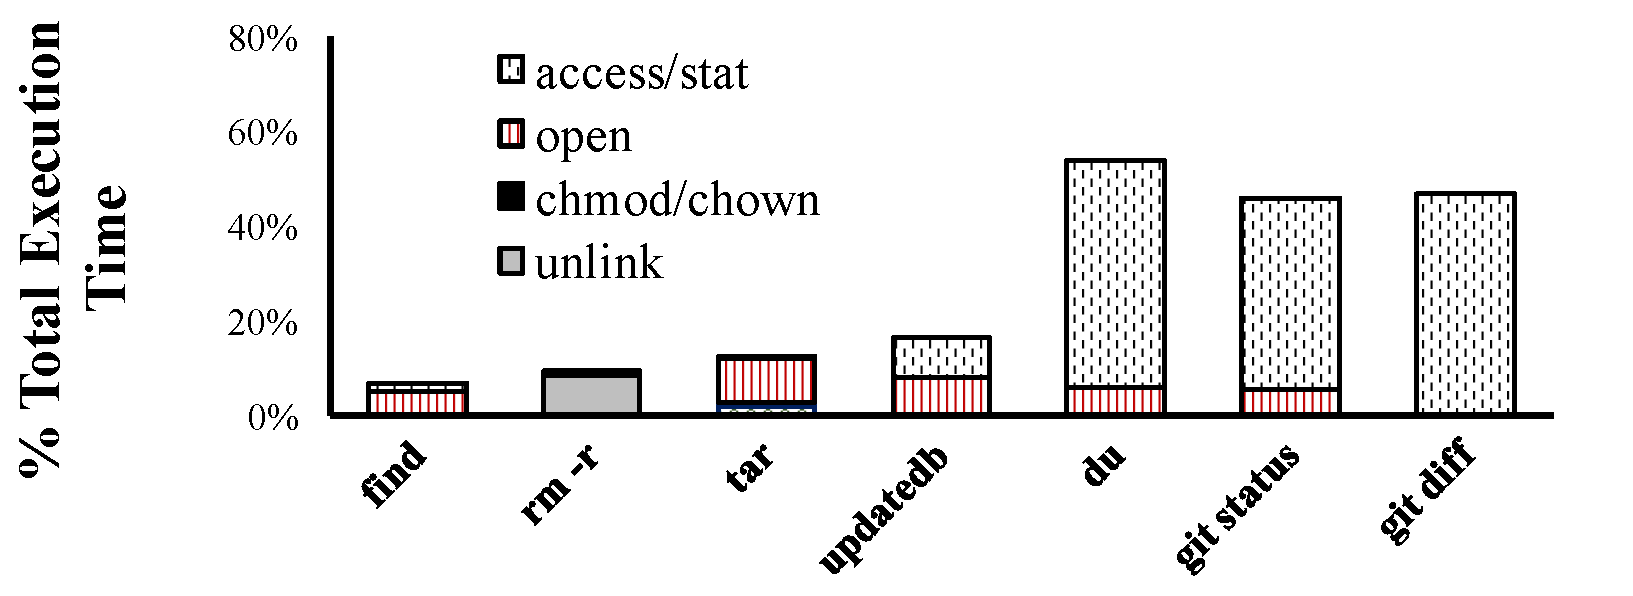
\includegraphics[width=5in]{dcache/plots/syscall-percentage.pdf} \\
\caption[Fraction of execution time on path-based system calls.]
{Fraction of execution time in several common utilities spent
executing path-based system calls with a warm cache, as measured with ftrace.}
\label{fig:dcache:lookup-frac}
%\vspace{-10pt}
\end{figure}

%\fixmedp{Please check these \% against time.  I think git diff is too high.  git status seems ok.}

Directory caches are essential for good application performance.
%Unix was designed such that ``(almost) everything is a file'',
%thus even accesses to in-memory file systems, device files, FIFOs and domain sockets
%first pass through the directory cache.
%In other words, 
Many common system calls must operate on file paths,
which require a directory cache lookup.
For instance, between 10--20\% of all system calls in the iBench system call traces do a path lookup~\citep{filenotafile}. 
Figure~\ref{fig:dcache:lookup-frac} lists the fraction of total execution time
%, as well as system time, 
several common command-line applications spend executing path-based system calls
(more details on these applications and the test machine in \S\ref{sec:dcache:eval}).
We note that these system calls include work other than path lookup,
and that these numbers include some instrumentation overhead;
% are coarse measurements that include  and work than path lookup;
%, and includes some time 
%for synchronous I/O (e.g., during {\tt rename}) as well as non-path tasks (e.g., creating 
%a file handle as part of {\tt open});
nonetheless, in all cases except {\tt rm},
the system call times and counts are dominated by
{\tt stat} and {\tt open}, for which 
%can be serviced from cache and for which 
path lookup is a significant component of execution time.
For these applications, path-based system calls account for 6--54\% of total execution time.
%and 25--77\% of system time.  
This implies that
lowering path lookup latency is
 one of the  biggest 
opportunities for a kernel to improve these applications' execution time.




\begin{figure}[t!]
\centering
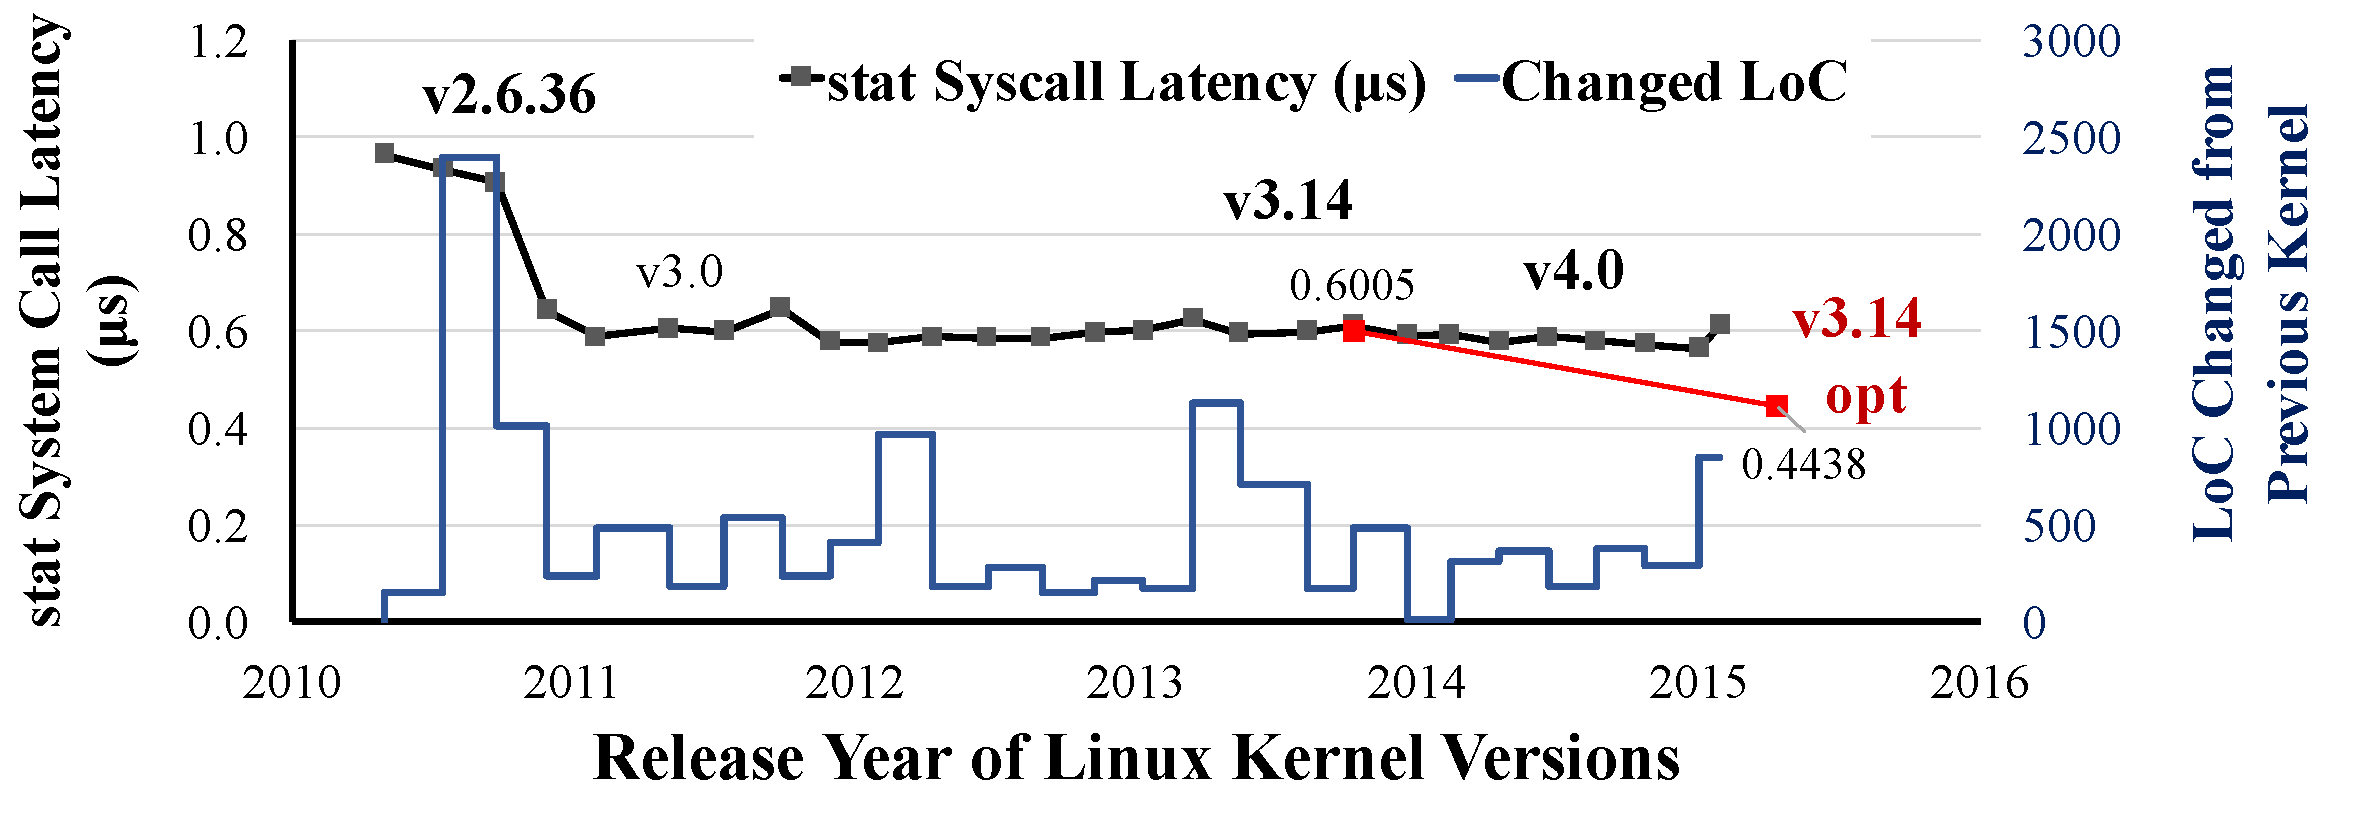
\includegraphics[width=6in]{dcache/plots/latency-by-version.pdf}
\footnotesize
\caption[Lantecy of {\tt stat} system call over years.]
{Latency of {\tt stat} system call with a long path {\tt XXX/YYY/ZZZ/AAA/BBB/CCC/DDD/FFF} on Linux over four years (lower is better), as well as the churn within the directory cache code (all insertions in {\tt dcache.c}, {\tt dcache.h}, {\tt namei.c}, {\tt namei.h} and {\tt namespace.c}). 
%Our optimizations significantly improve performance that has otherwise plateaued, despite significant ongoing developer effort.  
Our optimized \linuxver{} kernel 
further reduces {\tt stat} system call latency by \statspeedup{}\%.}
%\vspace{-15pt}
\label{fig:dcache:by-version}
\end{figure}


%\fixmedp{Add more evidence of lookup importance here: For instance, fraction of lookup time in file-related syscalls, or total lookup time in applications bound on file lookup latency.  }
Unfortunately, even directory cache hits are costly---0.3--1.1 \us{} for a {\tt stat} on our test Linux system, compared to only .04 $\mu$s for a {\tt getppid} and 0.3 \us{} for a 4 KB {\tt pread}. 
%\fixmetsai{Don, check this, I think read will be a better example, getppid is too trivial.}
This issue is taken particularly seriously in the Linux kernel community, which has 
made substantial revisions and increasingly elaborate optimizations to reduce the hit cost
of its directory cache, such as removing locks from the read path or replacing lock ordering with deadlock avoidance in a retry loop~\citep{corbet09jls,dcache-rcu}.
Figure~\ref{fig:dcache:by-version} plots directory cache hit latency against  lines of directory cache code changed 
over several versions of Linux, using a path-to-inode lookup \microbench{} on the test system described
in \S~\ref{sec:dcache:eval}.
These efforts have improved hit latency by 47\% from 2011 to 2013, but have plateaued
for the last three years.
%\fixmedp{if time, filter irrelevant changes from code deltas}
%at the cost of substantial developer effort.
%This latency appears to have plateaued 

The root of the problem is that the POSIX path permission semantics
seemingly require work that is linear in the number of path components,
and severely limit the kernel developer's implementation options.
%The root of this problem is that current directory cache
%designs reflect a straightforward implementation of the POSIX specification,
%which would seemingly require work that is linear in the number of path components.
For instance, in order to open file {\tt /\fnone{}/\fntwo{}/\fnthree{}} 
%for reading, 
one must have search permission
to parent directories {\tt /}, {\tt /\fnone{}}, and {\tt /\fnone{}/\fntwo{}},
as well as permission to access file {\tt \fnthree{}}.
The Linux implementation %of this specification is straightforward, 
simply walks the directory
tree top-down to check permissions.  
Unfortunately, when the critical path is dominated by 
walking a pointer-based data structure, 
including memory barriers on some architectures for multi-core consistency, 
modern CPUs end up stalling on hard-to-prefetch loads.
Moreover, because so many Linux features are built around this behavior, such as Linux Security Modules (LSMs)~\citep{wright+lsm},
namespaces, and mount aliases, it is not clear that any data-structural enhancements
are possible without breaking backward-compatibility with other Linux kernel features.
A priori, it is not obvious that a faster lookup algorithm, such as a single hash table lookup, 
can meet these API specifications and kernel-internal requirements; to our knowledge,
no one has tried previously.

%This paper proposes a decomposition of the directory cache, which allows
%most lookup operations to execute with a single hash table lookup (\S\ref{sec:dcache:dcache}),
%as well as optimizations to reduce the miss rate based on information that is {\em already in the cache}, but not used effectively (\S\ref{sec:dcache:readdir}).
%Our design maintains compatibility (\S\ref{sec:dcache:generalize}) through 
%several essential insights, including 
%how to separate the indexing of paths from checking parent permissions,
%and how to effectively and safely memoize the results of access control checks.


%% This paper proposes several new ways to organize a directory cache, which can yield 
%% substantial performance improvements over the current state of the art.
%% %This paper demonstrates that, despite this developer effort, there is still a substantial 
%% %missed opportunity hiding behind historical, intuitive, but not fundamental design choices.
%% Most of the Linux directory cache design reflects a straightforward implementation of the POSIX 
%% specification. %, with a division of labor that is suitable for mainstream file systems.

%This paper presents an alternative directory cache organization, which 
%improves performance by separating logical tasks, such as separating path indexing from permission checking; yet the design is sufficient to retain compatibility with POSIX.
%In the case of path lookup, 
%this paper demonstrates how 
%a per-component tree walk can be replaced with a single hash table lookup (\S\ref{sec:dcache:dcache}).
% without violating POSIX compliance.

%Our optimizations improve the performance of frequent lookup operations, but 
%introduce several costs, described in \S\ref{sec:dcache:dcache} and measured in \S\ref{sec:dcache:eval},
%which  we believe are acceptable and a net improvement for applications.
%First, these optimizations slow down infrequent modifications to the directory hierarchy, such as {\tt rename}, {\tt chmod},
% and {\tt chown} of a directory. 
%However, these slower operations
%account for less than .01\% of the system calls in the iBench traces~\citep{filenotafile}.
%Second,  the memory overheads of the dcache are increased.
%%(45\% per \dentry{}, as well as some  in our prototype).
%%(\fixmedp{XX MB} in our tests).  
%Third, lookup has a 
%probability of error from signature collisions that can be adjusted to be negligible
%%($2^{-141}$ in our configuration), 
%and within acceptable thresholds widely used by data deduplication systems~\citep{Debnath:2010:CSU:1855840.1855856, Srinivasan:2012:ILI:2208461.2208485, Quinlan:2002:VNA:645371.651321, Zhu:2008:ADB:1364813.1364831}.
%%, as well as how to remove
%%all memory barriers from the lookup path (\S\ref{sec:dcache:update}).
%In the micro-benchmark of Figure~\ref{fig:dcache:by-version}, our directory cache 
%optimizations improve lookup latency by 
%%revisions improve latency of accessing a long path
%%by 
%\statspeedup{}\% over unmodified Linux.
%%Our design addresses other missed
%%opportunities, such as identifying new opportunities to reduce the miss rate
%%through caching directory completeness.
%%\fixmedp{Do we want to highlight LoC?  3K is more than anything in the graph} \fixmetsai{Probably just mention in the evaluation. It's a metric that we should provide, but it's not awfully interesting.}
%%The total lines of code changed are fewer than 3,000 out of \fixmedp{XX}.
%%\fixmedp{Can we get 
%%, yet changes fewer than 3,000 lines of code.

%% SOSP cut - kind of long-winded
\begin{comment}
This paper rethinks current Linux directory cache design choices in light of the following goals:
\begin{compactitem}
\item {\bf Minimize the cost of a cache hit.} (\S\ref{sec:dcache:dcache}).
This means maximizing the benefit of temporal locality for frequent operations,
while pushing extra work of consistency maintenance onto less frequent, already-expensive operations.
%such as handling cache miss or updating massive metadata,
%in order to improve very frequent operations.
\item {\bf Maintain legacy compatibility.} (\S\ref{sec:dcache:generalize}).  Unix path semantics are complex, required by applications, file systems, and security modules, frustrating otherwise straightforward optimizations.  However tempting it may be to redesign path behavior to facilitate caching, path operations must exhibit the same behavior, with lower latency.
\item {\bf Never miss the same request twice in quick succession.} (\S\ref{sec:dcache:readdir}).  A number of less-frequent operations, such as reading a directory or secure temporary file creation, always miss in the cache {\em even if enough information is in cache to satisfy the operation.}  
%Of course, infrequent accesses should still be subject to a cache replacement policy, such as LRU.
\end{compactitem}
%Although directory caches must implement more complex semantics than a hardware memory cache,
%these principles should seem familiar to the reader with a basic architecture background.
%sadly, the Linux directory cache design violates all three.
\end{comment}

%This paper introduces several techniques to improve the performance of a directory cache,
%This paper explains several practical directory cache optimizations,
This paper demonstrates that these techniques improve performance for applications that use the directory cache heavily,
and the harm is minimal to applications that do not benefit.
%and that the worst case \microbench{} is only 12\% slower within \fixmedp{XX}\% of unmodified Linux.
%Each optimization we describe improves performance in isolation, and all can be combined.
%These optimizations change very few lines of code, and are backward-compatible with 
%legacy applications.  
%These changes are encapsulated in the VFS---individual file systems do not have to change their code.
%This paper describes a  prototype of these improvements implemented in Linux \linuxver{}.
%\S~\ref{sec:dcache:background} explains that the directory cache structure of Mac OS X, FreeBSD, and Solaris 
%are sufficiently similar that these principles should generalize.
%we compare and contrast Linux's directory cache
%with Mac OS X, FreeBSD, and Solaris in \S\ref{sec:dcache:background}, and explain inline how each
%optimization could be generalized to these other OS kernels.





%% \item {\bf Modularization and stackability}:
%% Any changes or optimizations must be implemented as modules inside Linux's VFS,
%% and can be stacked on top of the original design or any future optimizations. 
%% \item {\bf Backward compatibility}:
%% Any changes or optimizations must maintain least requirement of modifying any
%% file systems.
%% \item {\bf Generalization to other OSes}: Any changes or optimizations must be portable to other OSes with reasonable effort and change of design.




%% \dcache{} is proven to be effective on improving storage performance.
%% Experiments shows that,
%% in a Linux 3.x kernel, a \dcache{} with a xxx\% hit rate can speed up
%% metadata lookup and fetching time by xxx times.
%% \fixmetsai{experiment result, Linux version, and fs specs here}
%% However, we observed that Linux maintainers have made
%% constant and non-trivial efforts to improve \dcache{} in the Linux kernel.
%% We studied all \dcache{}-related source files in the Linux kernel Git repository,
%% and discovered that maintainers have committed
%% on average xxx revisions per source files.

%% We tested metadata lookup time on primary \dcache{}-related revisions.
%% Most changes on \dcache{} system only create xxx\%-xxx\% speed-up
%% than their predecessor.
%% \fixmetsai{result and graph here}.
%% Moreover, improvement to \dcache{} is still work-in-progress
%% for Linux maintainers.
%% \fixmetsai{reference to threads for latest dcache discussions}. 
%% All the evidences show that,
%% despite of significant reduction of storage operations,
%% efficiency of \dcache{} system internally still remains as a concern.

%% We argue that the design of \dcache{} needs to be carefully re-examined,
%% to fundamentally identify any missed opportunities that
%% improve value of \dcache{}.
%% At a high level, most optimization works for \dcache{} are focused on
%% improving ``how to cache'',
%% but we want to also lay eyes on ``what to cache'',
%% to ensure any valuable information returned from file systems
%% be captured by \dcache{} system.

%The contributions of this paper are as follows:
%\begin{compactitem}
%\item A performance analysis of the costs of path lookup and the opportunities
%to improve cache hit latency.
%\item A directory cache design that improves path lookup latency with a combination of techniques, including:
%  \begin{compactitem}
%  \item Indexing the directory cache by full path, reducing average-case lookup from linear to constant in the number of path components.
%  \item A Prefix Check Cache (PCC) that separates permission checking from path caching.  The PCC memoizes permission checks, and is compatible with LSMs~\citep{wright+lsm}.
%  \item Reducing the cost of checking for hash bucket collisions with path signatures.
%  \end{compactitem}
%\item Identifying opportunities to leverage metadata the kernel already has to reduce miss rates, such as tracking whether a directory is completely in cache.
%\item Carefully addressing numerous, subtle edge cases that would frustrate rote application of these techniques, such as integration with symbolic links and Linux namespaces.
%\item A thorough evaluation of these optimizations.  For instance, our optimizations improve throughput
%of the Dovecot IMAP server by up to \dovecotspeedup\% and latency of 
%updatedb by up to \updatedbspeedup{}\%.
%%git version control system by up to 25\%.
%
%\end{compactitem}

%\section{Background}
\label{sec:background}

This section summarizes \sgx{},
and current design points for running or porting applications on \sgx{}.
%and the legacy frameworks of porting 
%including \haven{}~\cite{baumann14haven}, \scone{}~\cite{osdi16scone}, and Panoply~\cite{shinde17panoply}. 


\subsection{Software Guard Extensions (SGX)}
\label{sec:background:sgx}

%\begin{figure}[t!]
%\centering
%\includegraphics[width=\linewidth]{figures/libosvssdk.pdf}
%\footnotesize
%\vspace{-0.3in}
%\caption{
%Comparison between libOS-based model (e.g., \haven{} and \graphenesgx{})
%and SDK-based (SDK for \sgx{}) model for migrating applications in enclaves.
%Green (light) boxes are trusted components and red (dark) boxes are untrusted.
%The libOS-based model often yields a larger TCB in the enclave,
%while the SDK-based model requires developers to be responsible of
%securing the enclave on the untrusted interface.
%}
%\label{fig:libosvssdk}
%\end{figure}

The primary SGX abstraction is an \emph{enclave}: an isolated execution environment within the virtual address space of a process.
The code and data in enclave memory do not leave the CPU
package unencrypted; when memory contents are read back into cache,
the CPU decrypts the contents, and checks the integrity of cache lines and the virtual-to-physical mapping.
SGX also cryptographically measures the integrity of enclaves at start-up, and 
provide attestation to remote systems or other enclaves.
%Remote entities can identify the owners of enclaves by distinguishing the cryptographic measurements
%generated with different signing keys.

%%% \sgx{} is a new feature on the 6th-genaration \intel{} CPUs.
%%% it contains a set of new x86/64 instructions, to initiate, destroy, and attest isolated execution environments (i.e., enclaves) in the address space of applications.
%%% When \sgx{} loads an application in an enclave,
%%% the code and data of the application will remain encrypted in the main memory,
%%% forbidding any mean to eavesdrop the application secrets.
%is a set of new x86/x64 instructions introduced
%to the latest \intel{} CPUs,
%to bootstrap an isolated execution environment
%inside applications' virtual memory address space.
%\sgx{} creates a memory region
%(generally referred as {\bf enclave}), storing both the code and data of the isolated execution,
%which stays encrypted in DRAMs and only the CPU is capable of encryption and decryption.
%The CPU derives the encryption key
%from the cryptographic measurement of the initial state of enclave memory,
%to allow remote entities to verify the soundness of execution and establish the trust
%needed for provisioning sensitive data.

\sgx{} enables a threat model where one only trusts the \intel{} CPUs and the 
code running in the enclave(s).
%whereas the rest of application, system software, off-CPU-package hardware devices and providers are untrusted. 
\sgx{} protects applications from three different types of attacks on the same host, which are summarized in Figure~\ref{fig:sgx-threats}: untrusted application code inside the same process but outside the enclave; operating systems, hypervisors, and other system software;
%\fixme{added Mona's suggestion}
other applications on the same host; and off-chip hardware.
A SGX enclave can also trust a remote service or enclave, and be trusted after inter-platform attestation~\cite{sgx-attestation}.




%%% \begin{compactenum}

%%% \item {\bf Inside process memory:}
%%% \sgx{} partitions the application process into two privilege levels, as the trusted part (in enclaves) which can access the whole process memory, and the untrusted part (outside enclaves) forbidden to access enclave memory.
%%% %the privileged part (in the  enclave region) can access all process memory,
%%% %while the unprivileged part (outside the enclave region) is limited to access only data that are not isolated by \sgx{}.

%%% \item {\bf From hosting OSes or hypervisors:}
%%% \sgx{} assumes that OSes and hypervisors can be compromised by either exploiting system vulnerabilities
%%% or malicious system software installed by administrators.
%%% Both types of compromise are legitimate threats to modern OSes, due to complexity of modern OSes and usage of public facilities like clouds.

%%% %Operating systems or hypervisors
%%% %that are either compromised by rootkits
%%% %or deliberately modified by the host providers.
%%% %An attacking host can access the raw data in DRAMs, or remap the
%%% %physical pages to other contexts.

%%% \item {\bf Physically from the hardware:}
%%% One type of attacks that cannot be defended by software-based solutions~\cite{flicker, criswell2014virtualghost}
%%% is from the attackers who have physical access to the hosts.
%%% \sgx{} can resist attacks on the host hardware
%%% including hacking peripheral devices like ethernet cards and connectors~\cite{hudson15thunderstrike}, tapping into buses, or eavesdroping DRAM data using Cold-boot attack~\cite{halderman09coldboot}.


%%% \end{compactenum}


%%% \sgx{} protects an application against unpredictable threats from both local and remote hosts.
%%% \sgx{} establishes a trusted path
%%% from one enclave to another,
%%% providing end-to-end protection to both enclaves to
%%% exchange data with confidentiality and integrity.
%%% %, processing the data and returning the computation results with end-to-end protection.
%%% We can further divide up the protection using \sgx{} into three elements:
%The use cases of \sgx{} mostly involve the process that an enclave
%retrieves a signed attestation from the processor,
%to exchange provisioning of critical information from remote servers.
%The purpose of such process is equivalent to
%expanding the trusted execution
%from remote servers
%to untrusted hosts,
%to harness resources such as CPU cycles and DRAMs.

%%% \begin{compactenum}

%%% \item {\bf Isolated execution:}
%%% \sgx{} guarantees the execution initiated in an enclave
%%% to be isolated from any part of the system except the enclave itself.
%%% %any part of the system except the enclave itself can access the execution state. 
%%% Achieved by the secrecy of encryption keys in \intel{} CPUs.

%%% \item {\bf Attestation of integrity:}
%%% Remote entities with a \sgx{}-enabled CPU can verify the integrity of an enclave, using the \intel{} Attestation Services (ISV)~\cite{isv}.
%%% %for its integrity of running the exact code that it is given.
%%% Achieved by the uniqueness of CPU keys to sign the cryptographic measurement of enclaves.

%%% \item {\bf Authentication:}
%%% Remote entities can identify the owners of enclaves by distinguishing the cryptographic measurements generated with different signing keys.


%%% %explicitly launched for processing the specific tasks, regardless of the identicality of execution.
%%% %That is, two mutually distrusting users can launch the same execution in  separate enclaves, yet be able to distinguish by the measurements as MACs (Message Authentication Code) signed by the users' private keys.

%%% \end{compactenum}


%One must note that \sgx{} only promises the integrity of application binaries
%initially loaded in enclaves.
%The gap between integrity of binaries and complete security has to be filled
%by ones who develop and approve the applications.
%More specifically, the clients are responsible of
%testing whether the applications contain any vulnerabilities
%that lead to information leak.
%To minimize the risk of leaving any flaws in the applications unintentionally,
%developers often tend to cut down the trusted computing base (TCB)
%of the applications. With smaller TCB, clients who launched the enclaves
%can more easily reason about the thoroughness of securing the execution.

%To achieve smaller TCB, the software development kit of \sgx{}
%intends to encourage developers to partition the applications and
%keep only security sensitive components in the enclaves.
%Such an intention is exactly contradicted by the trust model of \haven{},
%which must trust the loaded application as a whole.
%Except for the cases in which the whole applications must be secured,
%\haven{} actually downgrades the trustworthiness of enclaves.
%Figure~\ref{fig:libosvssdk} shows the comparison of the two models.


%%% By synthesizing and streamlining these three elements (i.e., isolation, attestation and authentication),
%%% \sgx{} provides a promising build block to securing applications
%%% from unpreditable security threats.

%developing applications
%that are resistant to unpreditable, unavoidable threats.
%Users expect \sgx{} to build up a wall for protecting the sensitive data, even against a catastrophic scenario like a complete takeover of the infrastructure.  

%\fixmedp{Explain how to read the figures in the captions. What do colors and shading mean?}
%
%\fixme{Disabled the whole discussion about SDK. dp: ok with me, but probably drop from figure} 
\begin{comment}
\subsection{The legacy framework (The \sdk{})}

{\bf Intel's \sgx{} SDK} (software development kit) for Linux~\cite{intel-sgx-sdk} is the official framework
for programming \sgx{} execution within Linux applications.
\sdk{} includes the components of two phases:
a {\bf compile-time utility} to generate a valid executable for running inside enclave,
and a {\bf run-time framework} to trigger the hardware-enforced isolated execution.
The two-phased design is based on the assumption that compilation of applications
is controlled by trusted, security experts,
to retain the trustworthiness of isolation model when running on untrusted OSes.


The work flow of \sgx{} programming using \sdk{} is as follows:
\begin{compactenum}
\item At the build-time (on trusted hosts), developers create a self-contained, static executable as the initial code and data after enclave creation.
We refer the executable as an ``enclave image''.
The enclave image is statically links with the enclave infrastructure, which provides enclave APIs (e.g., retrieving attestation) and a extremely small set of POSIX functions (e.g., {\tt memset()}).
After linking, the compile-time utility signs the executable and inserts the enclave signature structure
({\tt SIGSTRUCT}) in the application code.
\item At the execution-time (on untrusted hosts), the enclave image is taken by the framework. The user-space driver then requests enclave creation with the kernel driver, through {\tt ioctl()} to a pseudo-device {\tt /dev/isgx}.
The kernel driver creates and initializes an enclave using the authenticated signature structure,
and a token exchanged from an architectural enclave, {\tt AESMD}, for ensuring the validity of enclave. 
\end{compactenum}





%During the compile time,
%the developers create a self-contained, static binary, as the initial image of an run-time enclave (an ``enclave image'').
%\sdk{} provides the infrastructural libraries (libsgx) for static linking, which contain enclave APIs and few POSIX functions.
%A signing tool of \sdk{} will generates a valid enclave signature
%derived from the enclave image.
%Both the static linking and signing must happen on a trusted, development machine.


%After generating the enclave image, developers then ship it with the rest of application,
%to untrusted hosts (\sgx{}-enabled)
%where the \sdk{} run-time framework is installed.
%The run-time framework provides both kernel and user-space drivers,
%to interface \sgx{} hardware using the new x86 instructions (e.g., {\tt ECREATE}, {\tt EADD}, {\tt EENTER}).
%The framework also includes an architectural enclave (AESM), for validating the enclave attributes (and generating a run-time token),
%and a kernel EPC (enclave page cache) driver that manages paging for all running enclaves.



% includes both compile-time and run-time components:
%for the compile time, the SDK provides all the infrastructure libraries,
%which the applications statically link with,
%and a signing tool that generates the enclave signatures for hardware validation.
%The run-time framework then takes the signed enclave binaries,
%and uses the kernel and user-space drivers to initiate the isolated execution in enclaves.



\sdk{} centers the whole programming model based on the concept of partitioning an application,
and isolating only minimum application code in enclaves.
The partitioning minimizes the risk of compromising the enclaves,
due to smaller trusted computing base (TCB) and less opportunity of omitting security glitches.
With this model,
developers are expected
to identify the part of an application that performs the sensitive operations,
and define an validated interface to
the sensitive part and rest of the application.
\sdk{} encourages partitioning by reducing the difficulty of defining and accessing the interface---a language tool automatically generates the interface code with extra argument-sanitizing code.
The generated interface code essentially filters input and output of the enclave,
and prevents randomly copying memory across the enclave boundary, leaking or corrupting internal data.


%The Intel SDK has its limitations. The infrastructure of the SDK provides APIs in enclaves for accessing SGX features (e.g., attestation), as well as a small set of POSIX APIs
%(\roughly{}10 functions, such as {\tt printf} and {\tt memset}).


Despite that \sdk{} attempts to alleviate the difficulty of partitioning for SGX,
porting a piece of application code that is sophisticated and interactive to the rest of application
is still a significant cost to pay.
In general, developers want to find a reasonable granularity of partitioning---a ``sweet spot'' that partitions the application code neither too small nor too large, 
to nicely balance between frequency of enclave exits and risk of introducing incompatible code.
For an application written in C/C++, partitioning is cumbersome especially if the application is poorly modularized.


Unfortunately, the limited POSIX support in the \sdk{} infrastructure really strikes
the opportunity of fine-grained partitioning.
The lack of POSIX APIs in the infrastructure is fundamental, due to the restriction
on OS interaction from the enclaves.
The missing APIs encapsulates system calls, which can expose the enclave to some risky OS interaction model, such as {\bf Iago Attacks}~\cite{checkoway13iago}.

%In conclusion, this work targets on completing the API support, either at POSIX level or system calls,
%while retaining the isolation model.
%The platform can assist developers to refocus on partitioning applications for minimizing the risks.

\end{comment}

\subsection{SGX Software Design Space}

This subsection summarizes the principal design choices facing any 
framework for running applications on SGX.  We explain the decisions in
recent systems for SGX applications, and the trade-offs in this space.

\begin{figure}[t!]
\centering
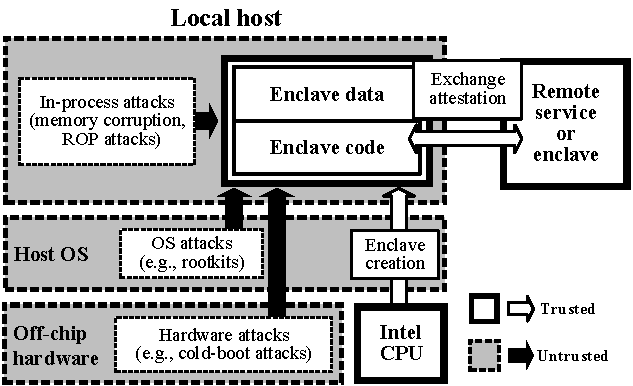
\includegraphics[width=.5\linewidth]{sgx.pdf}
\caption{The threat model of \sgx{}. \sgx{} protects applications
from three types of attacks:
in-process attacks from outside of the enclave,
attacks from OS or hypervisor, and attacks from off-chip hardware.}
% Red (dark) boxes are untrusted components and green (light) boxes are trusted.}
%For each enclave, \sgx{} establishes the chain of trust from the \intel{} CPU.
%Enclaves across physical machines or even infrastructures can remotely attest the integrity of execution, using the signatures generated and signed by the CPU.
%Green (light) boxes and arrows represent the trusted components and operations, and red (dark) boxes and arrows represent the otherwise.
\label{fig:sgx-threats}
\end{figure}

\paragraph{How much functionality to pull into the enclave?}
At one extreme, a library OS like Haven~\cite{baumann14haven} pulls most
of the application-supporting code of the OS into the enclave.
On the other extreme, thin ``shim'' layers, like SCONE~\cite{osdi16scone} and Panoply~\cite{shinde17panoply} 
wrap an API layer such as the system call table.
Pulling more code into the enclave increases the size of the TCB,
but can reduce the size and complexity of the interface, and attack surface, 
between the enclave
and the untrusted OS.

The impact of this choice on performance
largely depends on two issues. First, entering or exiting the enclave 
is expensive; if the division of labor reduces enclave border crossings, 
it will improve performance.
The second is the size of the Enclave Page Cache (EPC),
limited to 128MB on version 1 of SGX.
If a large supporting framework tips the application's working set size
past this mark, the enclave will incur expensive swapping.


\paragraph{Shielding complexity.}
SGX hardware can isolate an application from an untrusted OS, but 
SGX alone can't protect an application that  requires
functionality from the OS.  {\em Iago attacks}~\cite{checkoway13iago}
are semantic attacks from the untrusted OS against the application, where an unchecked system call return 
value or effect compromises the application.
Iago attacks can be subtle and hard to comprehensively detect, at least with the current
POSIX or Linux system call table interfaces.

Thus, any SGX framework must provide some {\em shielding} support, to 
validate or reject inputs from the untrusted OS.  
The complexity of shielding is directly related to the interface complexity:
inasmuch as a library OS or shim can reduce the size or complexity of the 
enclave API, 
the risks of a successful Iago attack are reduced.

\paragraph{Application code complexity.}
Common example applications for SGX in the literature 
amount to a simple network service running a TLS
library in the enclave, putting minimal demands on a shim layer. 
Even modestly complex applications, such as the R runtime and a simple
analytics package, require dozens of system calls providing wide-ranging functionality, 
including \syscall{fork} and \syscall{execve}.
For these applications, the options for the user or developer become: 
(1) modifying the application to require less of the runtime; (2) opening and shielding more 
interfaces to the untrusted OS; (3) pulling more functionality into a shim or a library OS.
The goal of this paper is to provide an efficient baseline, based on (3),
so that users can quickly run applications on SGX, and developers can 
explore (1) or (2) at their leisure.

\paragraph{Application partitioning.} An application can have multiple
enclaves, or put less important functionality outside of the enclave.
For instance, a web server can keep cryptographic keys in an enclave,
but still allow client requests to be serviced outside of the enclave.
Similarly, a privilege-separated or multi-principal application might create a separate enclave for
each privilege level.

This level of analysis is application-specific, and beyond the focus of this paper.
%which is on running unmodified applications in enclaves.
However, partitioning a complex application into multiple enclaves
can be good for security. In support of this goal,
\graphenesgx{} can run smaller pieces of code, such as a library, in an enclave, as well as
coordinate shared state across enclaves.

%* Partitioned vs. unpartitioned app?

%** Right choice depends a lot on whether the app has multiple principals or security concerns.

\begin{comment}
\fixmedp{Did a first cut at 2.2; needs to integrate the figure (or drop it).  I didn't know what to write for 2.3 yet.  I left the old text below for now (if there is anything you really want to save), but it needs to go away}

\subsection{Open Challenges}

\fixmedp{Here, I would give a taste of some of the issues we solve and why they are hard, like dynamic loading (and maybe fork or IPC).  Keep it short, a few paragraphs.}
\end{comment}

%\begin{figure}[t!]
%\centering
%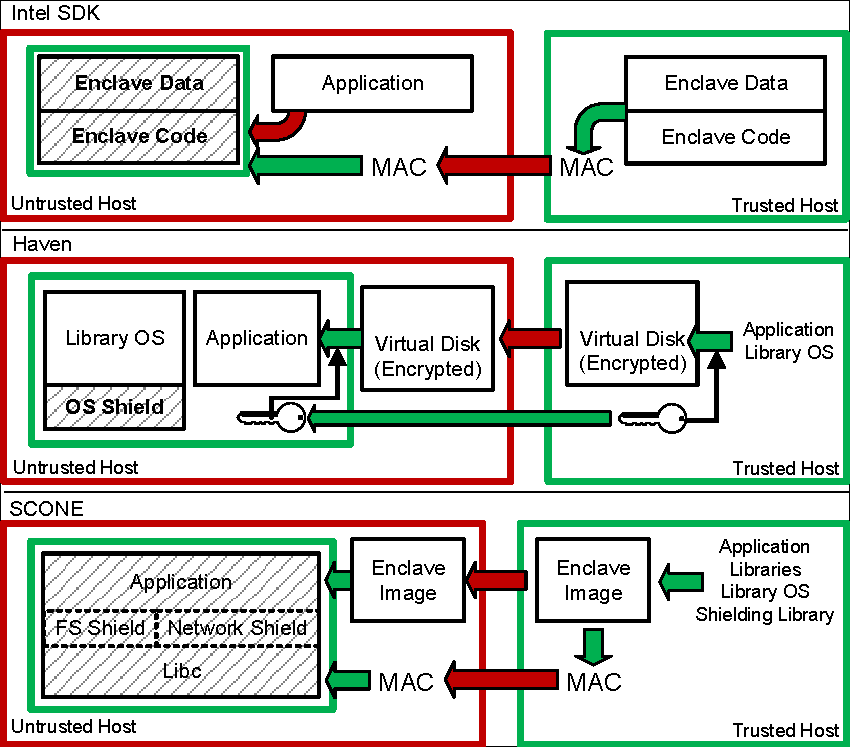
\includegraphics[width=\linewidth]{figures/sdkvslibos.pdf}
%\caption{Comparison of the code integrity model among different \sgx{} frameworks, including the \sdk{}, \haven{} and \scone{}.}
%%Green (light) boxes and arrows represent the trusted components
%%and operations, and red (dark) boxes and arrows represent the otherwise.
%%Patterned blocks represent the code and data included in the initial measurements of the enclaves.}
%\label{fig:sdkvslibos}
%\end{figure}


\begin{comment}
\subsection{\sgx{} shielding systems}
\label{sec:background:shielding-systems}




The current \sgx{} shielding systems, such as \haven{}~\cite{baumann14haven}, \scone{}~\cite{osdi16scone}, and Panoply~\cite{shinde17panoply}, enforce end-to-end isolation to
legacy applications without partitioning.
A \sgx{} shielding system preserves the trusted computing base (TCB)
of an application, and further increases it with a shielding layer to defend against the untrusted OSes.
By avoiding application partitioning,
%model of quarantining an unmodified, COTS application in an \sgx{} enclave.
a shielding system minimizes the effort of reprogramming the applications for \sgx{} execution, often with recompilation or packaging the binaries in an encrypted enclave.
%to merely recompiling or packaging the application code before signing it off for enclave execution.
%These \libos{}es internalize OS features into the enclave, to maintain a fixed-size,
%narrow interface to the untrusted host OSes.
%Porting applications using a \sgx{} \libos{} is vastly different from the programming model of \sdk{}---no programming effort is needed when porting with a \sgx{} \libos{}, and applications are isolated without partitioning.
In the following paragraphs, we compare the current shielding systems with the \graphenesgx{} approach.

\haven{}~\cite{baumann14haven} uses a \libos{} called \drawbridge{} in each enclave
to shield a single-process \emph{Windows} application from the untrusted host OS.
\haven{} absorbs the implementation of system APIs (i.e., Win32 APIs) from the host OS,
%\haven{} uses \drawbridge{}~\cite{porter11drawbridge} as the backbone of its enclave infrastructure, 
and exports a narrow enclave interface on which untrusted inputs are carefully filtered to defend against the Iago-type attacks.
Adding a \libos{} to each enclave causes a bloat of TCB---for \haven{}, the size of a \libos{} binary and shielding layer is \roughly{}200MB.
\haven{} has to establish the trust and integrity in all these binaries loaded into an enclave. Except that the shielding layer is a part of the enclave since its creation, \haven{} enforces the integrity of both the \libos{} and the isolated application,
by storing all binaries on an encrypted virtual disk and relying a remote, trusted server to provision the key for decryption.
\haven{} builds a trusted path from a remote server to local cloud machines,
to securely bootstrap application execution inside the enclaves.
%Other minor comparison between \haven{} and this work: the development and evaluation of \haven{}, at publication, is based on a simulated architecture.
%On the contrast, \graphenesgx{} is a released open-source platform, tested by many developers from institutes and corporations. \fixme{maybe bring up TCB?}



\scone{}~\cite{osdi16scone} isolates Linux micro-services in enclaves as a container-like environment.
After a brief attempt of building a \libos{} like \haven{},
\scone{} chooses a different approach of shielding the system API usage in applications, by designing shielding strategies based on each API.
\scone{} stacks the application on top of file-system and network shielding libraries, and extends a standard library C (musl~\cite{musl}) to securely exit the enclave for system calls.
Within the \sgx{}-aware Libc, \scone{} carefully filters the inputs from the host system calls, as the defend against known Iago attacks.
For instance, \scone{} ensures that pointers given to and returned by a host system call will point to addresses outside the enclave,
to prevent the host OS to manipulate pointers and cause memory corruption in the enclave.
\scone{} also authenticates or encrypts file or network streams
based on configurations given by the developers.


%The \libos{} implementation in \scone{} is based on musl~\cite{musl} and LKL (Linux kernel library)~\cite{lkl}.
%The design of a SCONE enclave (or Secure Container) has similarity
%with a basic block of \graphenesgx{}:
%they both validate input files based on cryptographic methods, and are fully configurable at a per-file basis.
%However, \graphenesgx{} supports a more complete set of Linux system APIs.
%The APIs that \graphenesgx{} especially contributes over \scone{} are the Linux multi-process APIs, including copy-on-write {\tt fork()}, {\tt exec()}, signals, and system V IPC (message queues and semaphores).

Panoply~\cite{shinde17panoply} further reduces the TCB of a shielding system over the SCONE approach, by excluding both a \libos{} and \libc{} from enclaves.
Instead, Panoply uses a shim layer shielding a portion of the POSIX API. The shim layer yields about 20 KLoC as its TCB (trusted computing base), which is much smaller than libc and/or a library OS.
% in other shielding systems.
As Panoply delegates the libc functions outside the enclave, its shim library defends the supported POSIX API,
including 91 {\em safe} functions and 163 {\em wild (unsafe)} functions.
Panoply also supports multi-process API including \fork{}, \exec{}, signaling, and sharing untrusted memory with inline encryption.
Compared to \graphenesgx{}, Panoply has made some different design decisions in supporting multi-process API,
including supporting fork by copying memory on-demand with statically determining memory access,
and using secured messaging for inter-process negotiating instead of coordinating over an encrypted RPC stream.




\subsection{Comparison and security implications}

\fixme{need to drop the SDK discussion, revisit the security claims, and discuss Iago attacks in details.}

Figure~\ref{fig:sdkvslibos} shows the comparison between \haven{}, \scone{}, Panoply, and \graphenesgx{}.
%The \sdk{} model uses a static MAC of the enclave code and data, given to the \sgx{} driver for bootstrapping the isolated execution.
The \haven{} model only initiates enclaves with the OS shield layer,
which unpacks the enclave binaries from a virtual disk---decrypted using a provisioned key.  
The \scone{} model extends the \sdk{} model---it statically links the application binaries with the shielding library, creating a static enclave image verifiable by its MAC. The \sdk{} and \scone{} model retain more flexibility in deploying and integrating \sgx{} enclaves by focusing on the code integrity rather than encryption.

The key concerns that affects users choosing among these solutions are {\bf trusted computing base (TCB) size} and {\bf attack surface}.
However, since all these solutions are based on different design decisions, assumption and requirements, the comparison of TCB size and attack surface is often imprecise and inconclusive.

\paragraph{TCB size.}
Most studies measure the TCB size of a system by the total LoC (lines of code) written for all the trusted components, or the size (in bytes) of all the trusted binaries.
The comparison of TCB size is only meaningful when two systems have comparable system features,
and are order-of-magnitude different in term of LoC or binary size.
For instance, the comparison of TCB size between \haven{} and \scone{} is never an apples-to-apples comparison.
The implemented system features and personalities
in these two systems are fundamentally different, and \haven{} supports a much larger fraction of Windows features than the fraction of Linux features supported by \scone{}.

We argue that the only occasion that the reduction of TCB size
can be convincingly demonstrated is when a design has partitioned a system into isolated components,
or removed unreachable execution paths.
For instance, the \sdk{} promotes application partitioning for \sgx{};
it requires additional partitioning effort but is effective for confining the TCB size.
By statically linking the application binaries
with the shielding layers and standard C library, \scone{} offers more opportunities in stripping the Libc and shield code of unused APIs, and thus reducing its TCB size.



\paragraph{Attack surface.}

Most studies estimate the severity of having an attack surface by the size of interface to the trusted and untrusted components.
The experience of \scone{} provides an important insight for estimating attack surface: the narrowness of interface is not proportional to the difficulty of defending against incoming attacks.
An interface overloaded with too many features or semantics can become a major source of vulnerabilities.

%\subsection{The \graphene{} Library OS}
%
%\graphene{}~\cite{tsai14graphene} introduces a \libos{} design that supports
%both single-process and multi-process Linux applications,
%but retains a narrow host interface (43 functions) as a vantage point for enforcing security isolation.
%The main contribution of \graphene{} is an distributed implementation of the POSIX namespace coordination,
%to support Linux multi-process abstractions across \libos{} instances.
%All the multi-process abstractions in \graphene{} is implemented using simple pipe-like RPC streams,
%without relying on any host memory sharing support.
%Based on this design, \graphene{} can easily isolate mutually untrusting applications,
%by blocking the RPC streams between unrelated applications.
%
%
%
%The design decisions made by \graphene{} are important keys to the \graphenesgx{} framework.
%First, the host interface contains mostly internal abstractions, and three external ones including files, network connections, and RPC streams.
%The simplicity of the host interface facilitates shielding the \libos{}
%from risky OS interaction.
%Moreover, \graphene{} implements multi-process abstractions across instances without memory sharing.
%\graphenesgx{} can rely on the distributed POSIX implementation
%to support multi-process applications across multiple enclaves, by coordination over validated RPC streams.


\end{comment}




\papersection{Background and Motivation}
\label{sec:background}

%\fixmets{1.5 page}

This section discusses the security features of  \sgx{}, and the challenges faced by developers that
intend to use \sgx{} for partitioning \java{} applications.
%the key challenges developers face when trying to manually partition applications using a technology such as \sgx{}.
%discuss the programming models and threats to security of \sgx{} enclaves.

\begin{figure}[t!]
\centering
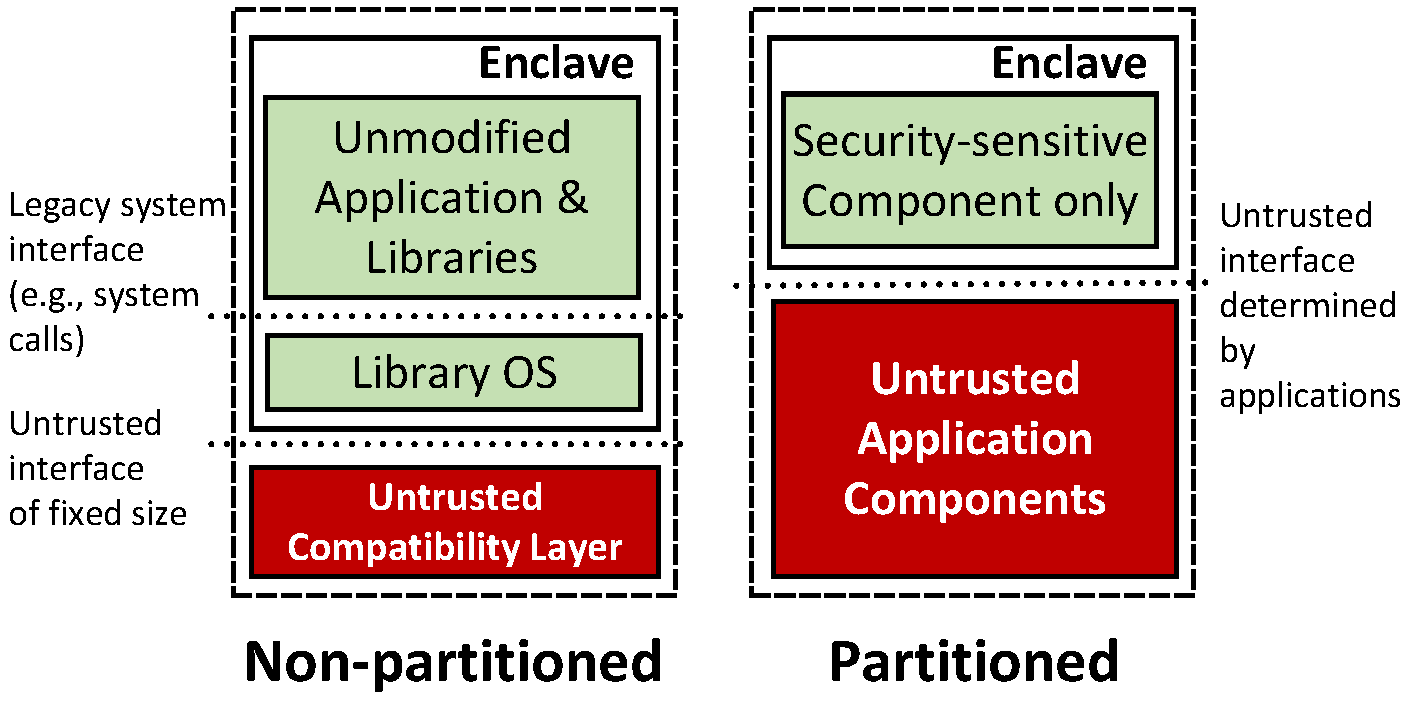
\includegraphics[width=1.0\linewidth]{libosvssdk.pdf}
\footnotesize
\caption{
Comparison between the Non-partitioned model (e.g., Haven)
and partitioned model for protecting applications in enclaves.
Green (light) boxes are trusted components and red (dark) boxes are untrusted.
The non-partitioned model yields a larger TCB in the enclave,
while the partitioned model requires developers to determine the untrusted interface at the enclave boundary.
}
\label{fig:libosvssdk}
\end{figure}

\papersubsection{\sgx{} Enclaves}

\intel{} \sgx{} ({\it Software Guard Extensions})
are a set of new x86/x86\_64 instructions
introduced in the \intel{} Skylake processor family.
Using \sgx{}, an 
application can designate part of its virtual memory as an {\em enclave}.
The CPU ensures that the contents of the enclave never leave the CPU package unencrypted.
The CPU also measures the integrity of a binary loaded into the enclave, and offers remote attestation,
similar to a TPM~\cite{TPM}.

%%% create a protected memory region, called an {\em enclave}, inside it's virtual memory,
%%% where it can load its security sensitive data with hardware-enforced isolation from the untrusted OS. 
%%% The processor with \sgx{}
%%% guarantees that any data loaded in enclave
%%% stays encrypted in the DRAM, by using a secret key deterministically derived from the application's cryptographic measurement and the CPU secret. 

\sgx{} is an appealing tool for protecting small amounts of highly-sensitive data or code, because it can defend 
against a malicious or compromised OS, hypervisor, or even hardware peripheral.
For instance, Hoekstra et al.~\cite{sgx-workshop1} show how \sgx{} can be used
to build a trusted path from a video chat application to a GPU and network card, which maintains confidentiality and integrity of the
video stream, even if the OS is compromised.
Similarly, because DRAM contents are encrypted, \sgx{} can resist attacks such as cold-boot attacks~\cite{halderman09coldboot} or 
malicious peripheral devices~\cite{hudson15thunderstrike}.

%\fixmedp{The flow from here to partitioned apps doesn't make sense.  Why are we getting into \sgx{} problems, then partitioned vs non-partitioned, then back to more problems?}
\sgx{} provides useful building blocks for secure applications, but does not
absolve the programmer of all responsibility for reasoning about end-to-end security.
Bugs in the application or supporting libraries can still disclose sensitive data from an enclave,
and porting code into \sgx{} can be subtle.
Inputs and outputs of an enclave must be checked carefully, and application-internal functions 
may not be hardened to the level of network-facing application interfaces.

Fundamentally, this argues for some combination of static analysis
and runtime monitoring of 
enclave code.  This is greatly simplified when the enclave code is written in higher-level languages
with properties 
%amenable to analysis.
%with type safety, memory safety, and other 
%that provide important 
%safety properties,
such as type safety or memory safety. %, thereby reducing the likelihood of these vulnerabilities.
Ideally, one would formally verify security properties of enclave code~\cite{moat}; this verification is significantly aided by using 
higher-level languages amenable to formal reasoning.
%Verification is significantly harder
%with C/C++ or assembly languages.


%The rest of this subsection outlines several pitfalls in partitioning an application for \sgx{}.



%\paragraph{Side Channels and Denial-of-Service.}
%In the current \sgx{} design, side channels are a significant concern, and are out of the scope of this paper.
%A controlled channel attack~\fixmedp{cite} can single step enclave execution by inducing page faults
%in the enclave.  \sysname{} does not specifically defend against side channel attacks,
%and we expect that any solution to this problem involves redesigning the %division of labor in virtual
%memory management for enclaves.

%Similarly, there is no guarantee that a compromised application will ever %enter
%an enclave.  Denial-of-service attacks are out of scope for this paper.

%% \paragraph{Writes outside of the enclave.}
%% However, the security of \sgx{} enclaves is founded on trusting the code running inside the enclave.
%% \sgx{} allows the trusted code to read and write data structures 
%% outside of the enclave.  Thus, it is easy for a developer to inadvertently write
%% code that discloses a secret, say by using a library that memoizes intermediate results to the untrusted heap.
%% A fundamental requirement is that developers must be able to reason about (or assert)
%% what code can and can't access data {\em outside} of the enclave.
%% \fixmedp{Can we say anything about whether such tools exist before Civet?}

%% %\fixmedp{Do I recall correctly that you can easily write to data outside of the enclave?  If so, this seems like something easy to get wrong, especially 
%% %if a library memoizes intermediate results.  The developer needs to be able to tell 
%% %Unless I am full of shit, can we paragraph-ize this fixme?

%% \paragraph{Vulnerabilities in the isolated applications.} 
%% One of the major threats to enclave security is the vulnerabilities in the isolated code,
%% such as memory corruption bugs,
%% control flow or information flows, semantic bugs, and so forth. 
%% %Moreover, although \sgx{} code integrity guarantees make enclaves resistant to code injection,
%% %an attacker may still manipulate control flow using code-reuse attacks~\cite{code-reuse-attacks}.
%% Moreover, recent research~\cite{hudata} shows that even with control flow integrity,
%% attackers can still manipulate the execution to leak the secrets through information flow.



%%% \sgx{} also proves the integrity of loaded binaries to remote trusted entities
%%% using mutual attestation based on a symmetric key generated from the measurements of communicating entities.
%%% \sgx{} usage model mostly involve the launched enclave mutually attesting the trusted host
%%% to obtain provisioning of security-sensitive information
%%% through a trusted channel. Such an execution model leverages resources such as CPU and DRAM from vulnerable untrusted \sgx{}-enabled hosts owned by cloud providers
%%% by extending the trust from
%%% the hosts owned and trusted by the clients or service providers.
%%% For instance, \sgx{} can isolate the decoder engine in an enclave
%%% after authenticating the customers to enforce Digital Right Management (DRM) even if the digital data is hosted on an untrusted cloud server.

%Use cases of \sgx{} mostly involve the launched enclave
%retrieving a cryptographically signed attestation from the processor,
%to exchange security critical information with remote servers through secured channels.
%The effect is equivalent to expanding the trusted space from remote servers
%to the local end, to harness local resources such as CPU and DRAM.

%One must note that \sgx{} only promises the integrity of application binaries
%initially loaded in enclaves.
%The gap between integrity of binaries and complete security has to be filled
%by ones who develop and approve the applications.
%More specifically, the clients are responsible of
%testing whether the applications contain any vulnerabilities
%that lead to information leak.
%To minimize the risk of leaving any flaws in the applications unintentionally,
%developers often tend to cut down the trusted computing base (TCB)
%of the applications. With smaller TCB, clients who launched the enclaves
%can more easily reason about the thoroughness of securing the execution.

%%% The key strength of \sgx{} enclaves over other software-based isolation framework such as
%%% {\em Flicker}, {\em Inktag} or {\em Virtual Ghost} is
%%% the ability to defend against attacks at the hardware level.
%%% These software-based solution often
%%% rely on a hypervisor below the OS to isolate the applications.
%%% If the hardware is attacked,
%%% the attackers may still bypass the software checkpoints,
%%% or directly steal confidential information from the DRAM.
%%% For \sgx{}, the only hardware included in the TCB is the CPU package,
%%% and in practice CPUs are believed to be hard to attack.
%%% Using techniques like cold-boot attacks~\cite{halderman09coldboot}
%%% to peek into DRAM content,
%%% or intruding the boot process using corrupted peripheral devices like Thuderstrike~\cite{hudson15thunderstrike}
%%% will affect any software-based isolation, but not \sgx{} enclaves.



%To achieve smaller TCB, the software development kit of \sgx{}
%intends to encourage developers to partition the applications and
%keep only security sensitive components in the enclaves.
%Such an intention is exactly contradicted by the trust model of \haven{},
%which must trust the loaded application as a whole.
%Except for the cases in which the whole applications must be secured,
%\haven{} actually downgrades the trustworthiness of enclaves.
%Figure~\ref{fig:libosvssdk} shows the comparison of the two models.

%%% In prior works using \sgx{} enclaves to secure applications,
%%% developers choose between two different programing models: the {\em library-OS-based} and the {\em partitioned} model (as shown in Figure~\ref{fig:libosvssdk}).
%%% In the libOS-based model, developers run the whole standalone,
%%% legacy application inside the enclave, using \sgx{} such as {\em Haven} or {\em \sgx{} libOS} to facilitate the rich OS features.
%%% The main benefit of using \sgx{} is that developers only have to employ minimal efforts to port any existing application.
%%% Even when designing new applications, developers bear no responsibility
%%% of identifying and reasoning about
%%% the security sensitive part of the application.

%%% However, when using libOS-based model, a sophisticated legacy application
%%% will yield huge trusted computing base (TCB) in the enclave,
%%% aggravating the risk of leaking information through vulnerabilities inside the enclave.
%%% Known bugs such as {\em the heart-bleeding bug} has shown that
%%% running security sensitive code like an encryption engine, and management code such as heart-beating service in the same address space
%%% can cause vulnerabilities that compromise the security by leaking the encryption key.
%%% As a result, using a partitioned model, developers can isolate only the most security sensitive components in an enclave,
%%% and leave the remaining code outside to minimize the TCB.

%%% Developers have to define the {\em untrusted interface} 
%%% to allow parts of a partitioned applications to interact.
%%% The untrusted interface is used either by the the untrusted components
%%% to trigger execution of the isolated components,
%%% or by isolated components to use untrusted rich OS features, such as networking for provisioning and sending the execution output to the remote hosts.
%%% Unlike the libOS approach that has a fixed untrusted interface (for different applications) at their interaction boundary with the OS,
%%% the width of untrusted interface for a partitioned application is up to developers' design.
%%% The \intel{} SDK for \sgx{} supports a set of syntaxes to specify the type and direction of flow for parameters of the untrusted interface, and enforces primitive
%%% type-checking of incoming values on transition to enclave.

%%% The trade-off between the libOS-based and partition model is based 
%%% on ease of development, the width of untrusted interface,
%%% and size of TCB.
%%% The benefit of the libOS-based model is that developers can save the effort
%%% of determining what to execute in the enclave,
%%% and whether the execution is safe,
%%% because the whole application is wrapped in the enclave.
%%% However, the risk of having vulnerabilities in the applications
%%% is not reduced, but in fact amplified due to the addition of
%%% the \sgx{} (e.g., the Haven binary yields around a few hundred MBs) to TCB.
%%% On the other hand, if the developers are willing to spend effort on carefully identifying the untrusted interface and re-designing their application around this interface, the partitioned model can improve security guarantees by minimizing the attack vectors.

%%% The goal of \sysname{} is to provide the benefits of both models.
%%% \sysname{} support a partitioned model
%%% for developers to isolate security-sensitive part of a \java{} application in enclave,
%%% and provide a language-based tool to automatically partition
%%% the minimal supporting classes to generate the enclave image.
%%% Even in the case where the isolated component need to frequently interact with the untrusted component or the OS,
%%% the language protection technique of information flow tracking
%%% guarantees that the secrets in the enclave are never leaked
%%% without the developers explicit consent. 


\papersubsection{Two \sgx{} Usage Models}
\paragraph{Non-partitioned applications}
One model for using \sgx{} is to run an entire application in the enclave.
This is exemplified by Haven~\cite{baumann14haven}, which runs a \win{} application and all supporting libraries
on top of a library OS (\libos{}) inside an enclave.  This approach is illustrated on the left side of Figure~\ref{fig:libosvssdk}.
The non-partitioned model offers simple deployment, requires no application changes, and can provide practical benefits, 
such as protecting an application from an untrusted cloud hypervisor.
In the case of Haven, running an unmodified application bloats the TCB by 5.5 billion lines of code.
%By pulling millions of lines of extraneous code into an enclave, there is a significantly increased risk 
%of vulnerabilities that disclose
%sensitive data, such as Heartbleed~\cite{heartbleed}.
%\fixmebj{Move heartbleed example to next subsection for motivation.}


\paragraph{Partitioned applications}
One can reduce the in-enclave trusted computing base by paring it down to only the
security-sensitive pieces of application logic (right side of Figure~\ref{fig:libosvssdk}).
%This paper focuses on a second usage model for \sgx{} enclaves, where an application is partitioned into
%the untrusted and trusted sides 
%Only sensitive data and computation are placed inside the enclaves.
This partitioned model requires the developers to
identify what in the application should be protected; harden an interface between trusted and untrusted components; 
%modify the application source;
and reason about potential information flows at the enclave boundary~\cite{kilpatrick2003privman}.
This effort can be non-trivial and subtle, but for application developers motivated by interests such as 
regulatory compliance or competitive advantage in business, the additional effort can yield a much smaller trusted computing
base (TCB), and thus a reduced attack surface.
A key goal of \sysname{} is to minimize the developer's effort to partition an application---both in lines of 
code changed, and in leveraging language analysis to reason about narrow points in the application's data and control flow at
which to establish an interface between trusted and untrusted components.


%\fixmebj{Talk about protecting untrusted app from os or hypervisor is orthogonal.}



\papersubsection{Challenges in Partitioning \java{} Applications on \sgx{}}

Using a higher-level language can be useful to reduce the risk of semantic errors in an application,
yet there are several fundamental, technical challenges to using a managed language, like Java,
in an \sgx{} enclave.
In part, this is simply an artifact of the \sgx{} design, which is designed
for native libraries.
%To our knowledge, no previous work has successfully executed a \jvm{} inside an enclave.

%% For developers who prefer implementing applications in a higher-level language like \java{} ---
%% to limit the vulnerabilities in the applicatins,
%% and use the partitioned model to protect the applications with \sgx{}
%% --- to reduce the TCB of enclaves,
%% the combination of two protections can be challenging.
%% For starter, \sgx{} enclaves are not designed to run any applications that are not native binaries.
%% Even though using the non-partitioned model with a \sgx{} like Haven
%% can potentially run \java{} applications with the whole \jvm{}
%% inside the enclaves,
%% the technical effort required is non-trivial,
%% and no previous work has demonstrated any successful case yet.
  
%% \paragraph{Introducing \sgx{} to \java{}.}
%% We identity several challenges in presenting the \sgx{} protection to
%% \java{} applications, to allow them to isolate their security-sensitive components.
%% The challenges are in fact more than just the technical efforts
%% to design a wrapper API for \sgx{} instructions.
%% The fundamental gap between the requirement of using \sgx{} enclaves
%% and the characteristics of the \java{} language
%% is the primary pitfalls in combining them.
%% The requirements are not limited to \java{} and \sgx{},
%% but can apply to other languages and hardware protections.
%% \fixmets{The discussion of the three primary problems must match section~\ref{sec:concept}.} 


%%% \sgx{} enclaves provide strong isolation guarantee for applications,
%%% against the malicious or vulnerable application components, system stack,
%%% and hardware (except the CPU itself).
%%% However, the security guarantees of the \sgx{} enclave is dependent on whether the developers design perfect applications without exploitable vulnerabilities that may compromise the application's security.
%%% As the application developers are not perfect,
%%% even applications or components isolated in enclave can face threats to their security.
%%% As follows, we discuss a few potential threats
%%% to the enclave security,
%%% even under the assumption that the \sgx{} hardware is implemented as completely secure --- which can be another threat otherwise. 

%\fixmedp{I roughly want the rest of this section to have a problem, explanation, solution structure, with the overall theme being that this is subtle and we really need some analysis tools to get this right}


%% \paragraph{Applications are not perfect} 
%% The \sgx{} hardware cannot prevent applications from copying secrets out of the enclave without limiting functionality.
%% The trusted isolated components can copy any sensitive data from the enclave to the unencrypted memory, and potentially leak the enclave secrets.
%% The primary risk in the isolated components
%% is often memory corruption vulnerabilities, such as buffer overflow,
%% %Because in enclave applications can access any part of out-of-enclave memory unrestrictedly,
%% prevalent in applications that are not implemented in type-safe languages.

%% The best known technique to prevent vulnerabilities is to model the applications and verify them using {\em formal verification}.
%% While Sinha et.al.,~\cite{moat} use formal verification to prove confidentiality of enclave programs, it is impractical to accurately model complex sophisticated applications.
%% As a result, in addition to formal verification, maintaining smallest TCB
%% in the isolated components is the most practical approach 
%% to ensure enclave security,
%% and is the main reason to choose partitioned programming model over
%% libOS-based model.


%\begin{figure}[t!]
%\centering
%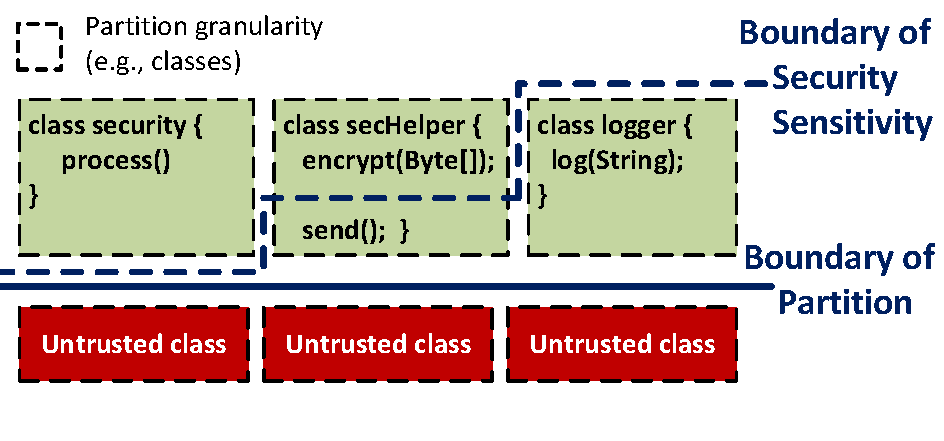
\includegraphics[width=\linewidth]{figures/partition.pdf}
%\footnotesize
%\vspace{-0.3in}
%\caption{
%Partitioning --- either manually or by automated tool ---
%often causes wider boundary of partition than the actual security sensitivity boundary
%due to (a) design granularity : {\tt SecHelper} contains a {\tt send()} method that is not partitioned from the rest of the class by design.
%or (b) better performance :  the less security sensitive {\tt logger} class is kept in 
%the privileged level to service frequent method calls. \fixmebj{Initial letter of all 
%class names must be Capital.}
%}
%\label{fig:partition}
%\end{figure}

%However, even if developers partition the applications and run only
%security sensitive components in the enclave,
%the developers may still leave some code irrelevant to
%enclave secrets inside the enclave.
%The reasons of having more-than-minimal TCB in enclaves
%are often that developers have to partition code in the granularity of source files or functions,
%or developers have to import more code to limit the width of interface and
%the frequency of interaction with the untrusted code.

\paragraph{\bf Challenge I---Cleanly partitioning classes and objects (\S\ref{sec:concept:partition})}
Java encapsulates the placement of object data and code within virtual memory, which facilitates features
like inheritance and garbage collection, but complicates integration with \sgx{}.
To program for an \sgx{} enclave, the developer must understand which regions of virtual memory 
are in the enclave, and which are outside of the enclave.
Note that \sgx{} allows code in the enclave to access memory
outside of the enclave.  Thus, it is easy for a developer to inadvertently write
code that discloses a secret, say by using a library that memoizes intermediate results to the untrusted heap.
Further, when a Java class inside of an enclave inherits methods or fields
from a parent class that is placed outside of the enclave, it is easy to 
inadvertently pass sensitive inputs to a function outside of the enclave,
or update a class field outside of the enclave.

In order for programmers to be able to sensibly program for \sgx{}, they need
a model of how objects are placed inside and outside of the enclave at runtime, as well as a model
for if and when updates to objects are propagated across the enclave boundary.
%\fixmedp{please fact check this rewrite, and make sure I am on the right track}
%\fixmebj{Looks ok to me. I will let Chia-che remove the fixmes.}
%% \sgx{} enclaves isolate the trusted components from the rest of the application,
%% and makes sure that no code or data
%% is shared between the trusted and untrusted parts.
%% For languages like C, which statically define functions and variables, it is easier for developers to cleanly
%% draw the line between trusted and untrusted components.
%% However, for a managed language like \java{}, a class can be inherited by other classes,
%% or referenced as other classes's fields, so the class may belong to both
%% untrusted and trusted components.
%% As a result, developers may struggle to manually partition the \java{} classes, especially if large portions of the classes are imported from libraries and not written by themselves.

%Reasoning about where in a program to draw the line between 
%trusted and untrusted code is subtle.
%On one hand, the developer has an incentive to minimize the size of the 
%API between the enclave and untrusted code, as well as an incentive to
%minimize the total code in the enclave.  These goals can sometimes be at odds.
%Each entry and exit to an enclave has a cost roughly comparable to a
%process context switch\fixmedp{right?}; an easy way to reduce enclave entries and exits is to simply 
%pull more code into the enclave, which increases the size of the TCB. For instance, in Figure~\ref{fig:partition}, even if the class {\tt Logger} is not security sensitive, 
%it is included in the enclave side of boundary of partition to avoid frequent entries and exits out of enclave.


%\fixmedp{I'm not sure how to explain Figure~\ref{fig:partition}, but it needs an explanation.}

%Fundamentally, the art of paritioning an application is to find a ``pinch point'' or
%``narrow waist'' in the application, where there is a natural point to insert an API and 
%security checks.  This is indeed as much art as science, often done manually by experts\fixmedp{any more supporting evidence or cites?}. Moreover, different classes of applications in managed languages like \java{} are tightly coupled; and it is necessary  to widen the boundary of partition to include some non-sensitive code in the trusted component.
%For instance, in Figure~\ref{fig:partition}, even if the {\tt send()} method is not security sensitive, it has to be included in the enclave code because of the design of the class {\tt SecHelper} to achieve a clean partition of the application.
%It is unlikely that the average developer will successfully navigate this design process without analysis tools, such as \fixmedp{examples?},
%to help identify these natural division points.


%% Experts can use a manual partitioning technique to achieve smallest TCB for the isolated components compared to automated tools.
%% However, the manual partitioning costs a lot of effort,
%% and rare expertise, lack of which can cause larger TCB.

%% Neither manual nor automated partitioning is perfect:
%% the resulted boundary of partitioning often has a gap from the actual boundary of security sensitivity (as shown in figure~\ref{fig:partition}),
%% leaving more code in the privileged level
%% than what's actually needed.
%% Having the gap between the ideal and resulted boundary
%% is mostly inevitable, due to multiple reasons.
%% One common reason is the granularity of partitioning,
%% which can vary from a binary file, a component, a source file,
%% a class, a method (a function) to a line of code.
%% Another reason is that a component or a method may be too frequently called
%% by the security sensitive code,
%% laying the boundary between the component or method from the security sensitive side may bring too much overhead or risk,
%% because the execution crosses the boundary too often.
%% Therefore, developers often will balance among the effort of partitioning,
%% risk or cost of communicating between different partitions,
%% and minimizing the TCB in the security sensitive parts.

%\fixmedp{Maybe move the commented paragraph below down into the design section?  I'd like to downplay the plugs for our work here, and instead fulfill these promises later}
%% \sysname{} automates partitioning of applications,
%% based on the boundary at the classes which the developers marked
%% as the interfaces of the enclave.
%% Only the classes that are depended by the marked classes
%% will be included in the enclaves,
%% to minimize the TCB.
%% Although not all classes pulled into the enclaves
%% are necessarily security sensitive,
%% the enclaves are protected from the potential vulnerabilities in those classes,
%% by the security guarantees of \java{} language,
%% and the information flow tracking in \sysname{}.

%Another threat to \sgx{} is the vulnerability of the 
%security sensitive code running in the Enclave. The 
%main guarantee of \sgx{} to isolate the secure data 
%from other components and privileged OS is undermined 
%if the Enclave code can be tricked to leak the 
%security sensitive data to the attacker. Executing 
%buggy code in \sgx{} enclave can inadvertently leak 
%information if the attacker can exploit memory-safety 
%vulnerabilities like buffer overflow and dangling 
%pointers.  

% Cumbersome and approximation to partition code
%The developers have to manually partition their code 
%into security sensitive and insensitive part. If this 
%partitioning is done by a novice developer, some of 
%the security insensitive parts of the application can 
%end up in the security sensitive part, increasing the 
%Trusted Computing Base(TCB). Moreover, the 
%partitioning of code is not straightforward, which 
%can also contribute to a less stricter TCB. The bigger the TCB, the more %vulnerable is the Enclave code to attacks.

% Buggy Code leads to inadvertant information leakage


% \sgx{} code only Integrity protected not confidential
%Moreover, \sgx{} only protects the integrity of the enclave code. The security critical part of the application is stored in plaintext while the secret data is provisioned securely after attestation. However, \sgx{} does not protect the confidentiality of enclave application code which may be executing a secret algorithm. \fixmebj{Talk more about the problem motivating security tag preservation.}
%\sgx{} can natively guarantee either code integrity or
%code confidentiality (as part of the enclave data), but not both.
%If application code is included in the enclave measurement and
%verified by the hardware,
%the code must stay in plaintext as part of the enclave image.
%If any code is stored or provisioned in encrypted forms,
%the application or infrastructure in enclave must dynamically load
%the code after decryption.
%Supporting dynamic loading makes enclaves open to code injection
%if the applications have exploitable vulnerabilities.

\paragraph{\bf Challenge II---Dynamically loading byte-code with integrity (\S\ref{sec:concept:loading})}
\sgx{} establishes trust by verifying the integrity of the code in the enclave.
Therefore, enclaves must be bootstrapped with static, native binaries.
%that have consistent measurements.
However, \java{} classes are shipped as byte-code,
and dynamically loaded by \jvm{}s.
The subtle security challenge for a Java developer 
is ensuring that, when a class is dynamically loaded into an enclave, by passing a string name of the class,
the application needs to be able to verify that this is a trusted class file
and that the initial state of the class is correct.
Thus, we introduce techniques to manage trust and verify the integrity of 
dynamically loaded code, including encrypted class files.

We note that using byte code is both a liability and opportunity.
One could pre-compile byte code to native code on a trusted host, and simply run the signed native code.
However, this foregoes the opportunity for performance-critical enhancements
such as profile-guided optimization or heap management optimizations for
smaller heaps.  Version 1 of \sgx{} only has up to 128 MB of total enclave page cache;
Version 2 will relax this extension.  As long as \sgx{} is a moving target,
we expect there will be value in the ability to dynamically optimize the
in-enclave code for the constraints and application behavior at runtime.

%This means the \sgx{} enclaves can only guarantee the code integrity of the initially loaded infrastructure, which in turn has to
%verify the integrity of classes dynamically loaded.
%\fixmedp{Can you say a bit more about why this is hard or interesting?}

%The hardware-level \sgx{} code integrity mechanism is based on a cryptographic
%signature of a static binary in plaintext.
%If any application dynamically loads any code after the enclave's initial measurement,
%the initial application must be trusted to attest the loaded code.
%The subtle tension is that there is no way to protect the confidentiality of
%a secret algorithm, except by dynamically loading an encrypted binary.
%Dynamically loading code increases the risk of code injection attacks and other control flow compromises. The interpreted and managed languages effectively compound the
%risks by dynamically loading all the application code.

%Any application partitioning solution that protects sensitive algorithms and data
%must have a robust dynamic loader that can measure encrypted libraries or classes.
%\sysname{} includes a loader that can measure encrypted class files,
%provisioned from a trusted host.

%% \sgx{} enclaves require code integrity in the isolated applications.
%% If the code integrity is not maintained, adversaries can corrupt the enclave code to
%% force the applications to leak the information provisioned from the remote,
%% trusted hosts.
%% \sgx{} hardware only guarantees
%% the integrity of the code initially loaded into the enclaves.
%% However, if an application choose to dynamically
%% load any code after the enclave starts,
%% the application is responsible for the integrity of the code loaded.
%% The fact that dynamic loading of applications, libraries or components
%% is a feature that can potentially make enclaves vulnerable and open to code injection,
%% raises concerns against supporting managed languages in the enclaves.

%% On the other hand, code confidentiality can be a desirable feature,
%% for application developers who prefer keeping the secret sauce of their algorithms concealed.
%% To enable the feature of code confidentiality in enclaves, the protected code must be dynamically loaded into the enclave,
%% because the \sgx{} hardware only accept
%% the initial loaded code to be in plaintext.
%% \sysname{} provides both code integrity and confidentiality by verifying
%% every classes dynamically loaded into the enclaves,
%% and allows loading classes provisioned from trusted hosts.


%% In general \sgx{} enclaves are prone to having side channels, such as timing channels. Because \sgx{} relies on the untrusted OS for paging,
%% an enclave will always leak page fault addresses, except the lower 12 bits (offsets in pages).
%% Such a leakage gives the untrusted OS to amplify the side channels,
%% by forcing page faults on every instruction or memory access.
%% This so-called {\em Controlled Channel Attack} is common to all applications who use \sgx{} protection, regardless of the programming models.
%% \sysname{} does not specifically defend against side channel attacks.

%% \paragraph{Denial-Of-Service Attacks}
%% \sgx{} is not designed to be safe against denial-of-service attacks.
%% Because the untrusted OS still controls the host resources,
%% there are countless ways to prevent an enclave from making progress.
%% For example, the OS can simply starve the enclaves by
%% never scheduling CPU, memory or other resources to the enclaves.
%% \sysname{} does not specifically defend against denial-of-service attacks.

\paragraph{\bf Challenge III---Seamless access of in-enclave objects (\S\ref{sec:concept:accessing})}
Java code outside of the enclave must be able to call enclave entry points and 
have some notion of objects that are inside the enclave.
Unlike C, where most function addresses are determined once
at the dynamic linking phase,  Java identifies most functions through
object references (e.g., {\tt Foo.toString()}).
Thus, the untrusted code must be able to reference
objects inside of the enclave in a way that makes sense when
the untrusted code behaves correctly, but that does not create unexpected information flows 
out of the enclave.
Similarly, the developer needs a constructor interface to declare which dynamically-created
objects should be placed in the enclave and which should be outside of the enclave. 


%% For native binaries, enclave entry points are statically inserted
%% into the untrusted code
%% at explicit locations known to interact with the enclaves.
%% However, for \java{} applications, instantiating or calling methods
%% on isolated components must dynamically trigger enclave entry.
%% For instance, calling the {\tt toString()} method of any object 
%% may trigger enclave entry based on whether the object's reference type is in the enclave.
%% Moreover, the the objects and methods determine the entry targets (the locations where the execution transfer after entering the enclaves) and the arguments passed into the enclaves at entry.
%% Unlike native binaries, the code behavior at enclave entry must be determined at runtime.
%% \fixmedp{I don't understand this point yet.  Is the issue that the untrusted code needs to track
%% opaque references into the enclave?  Can you explain more?}


%The \sgx{} hardware ensures that the enclave only has fixed number of entry points 
%(exactly one location where the execution starts, but multiple pre-defined locations 
%that the execution can jump to). However, for an application written in a language like JAVA with a virtual machine or interpreter, there are no clear entry points separating 
%the trusted and untrusted components. Moreover, due to the approach of executing intermediate code, it is also difficult to determine the entry points at runtime.

%Just separating an application into parts based on security sensitiveness is not enough to securely isolate the two parts using \sgx{}. In addition to application partition, there is a need to automatically determine the entry points without offloading the effort to the developers. \sysname{}  automatically identifies and exports all untrusted interfaces to the isolated classes at build time.

%\paragraph{Discussion.}
%This section has outlined several pitfalls for developers of partitioned applications.
%These common pitfalls render the hardware protections of \sgx{} useless.
%Language-level analysis can automate error-prone reasoning in the best case, or, in the worst case, 
%can at least offer invaluable guidance to the developer.  For \sgx{}-style
%hardware to be useful to a wide array of developers, developers need language-level
%tools that can also factor in hardware-level protection mechanisms.

\begin{comment}

\papersubsection{The Challenges of Combining Language and Hardware Protections}

Language and hardware protections provide varying benefits
to application security:
Languages improve the internal security inside the applications,
while hardware provides the base defenses that cannot be easily overridden or bypassed.
Commonly security experts exploits both types of protections
to further harden the security of applications.
For example, hardware protections may take information from the language runtimes or compilers to enforce the security policies,
or language protections may rely on hardware protections to bootstrap the initial trust they need. 

However, the combination of language and hardware protections is more
like a trick of the trade for security experts:
the use of hardware protections is deeply buried in the design of language protections,
so that users (application developers) lose direct access
to the security guarantees and features provided by the hardware.
\fixmets{Think of an example: Maybe TPM.}
The approaches of combining language and hardware protections are mostly ad-hoc to the use cases,
i.e., how one protection is used to improve or reinforce another.

There are two reasons for why combining language and hardware protections
is so inevitably hard.
First, hardware protections often have restrictions
on the languages that must be used
to access the security guarantees and features of the hardware.
For example, \sgx{} requires the loaded code to be implemented in C or C++,
or any languages that can compile applications into static binaries.
The restriction is not simply a design decision
made by the hardware or its SDK,
but a result of the fact that \sgx{} requires a static image to guarantee the integrity of execution.
On the other hand, if the language used is a managed language like \java{},
accessing \sgx{} hardware will be cumbersome,
because it is hard to provide any APIs to allow direct access to the \sgx{} hardware,
to harvest its security guarantees
or to utilize its features.

\begin{figure}[t!]
\centering
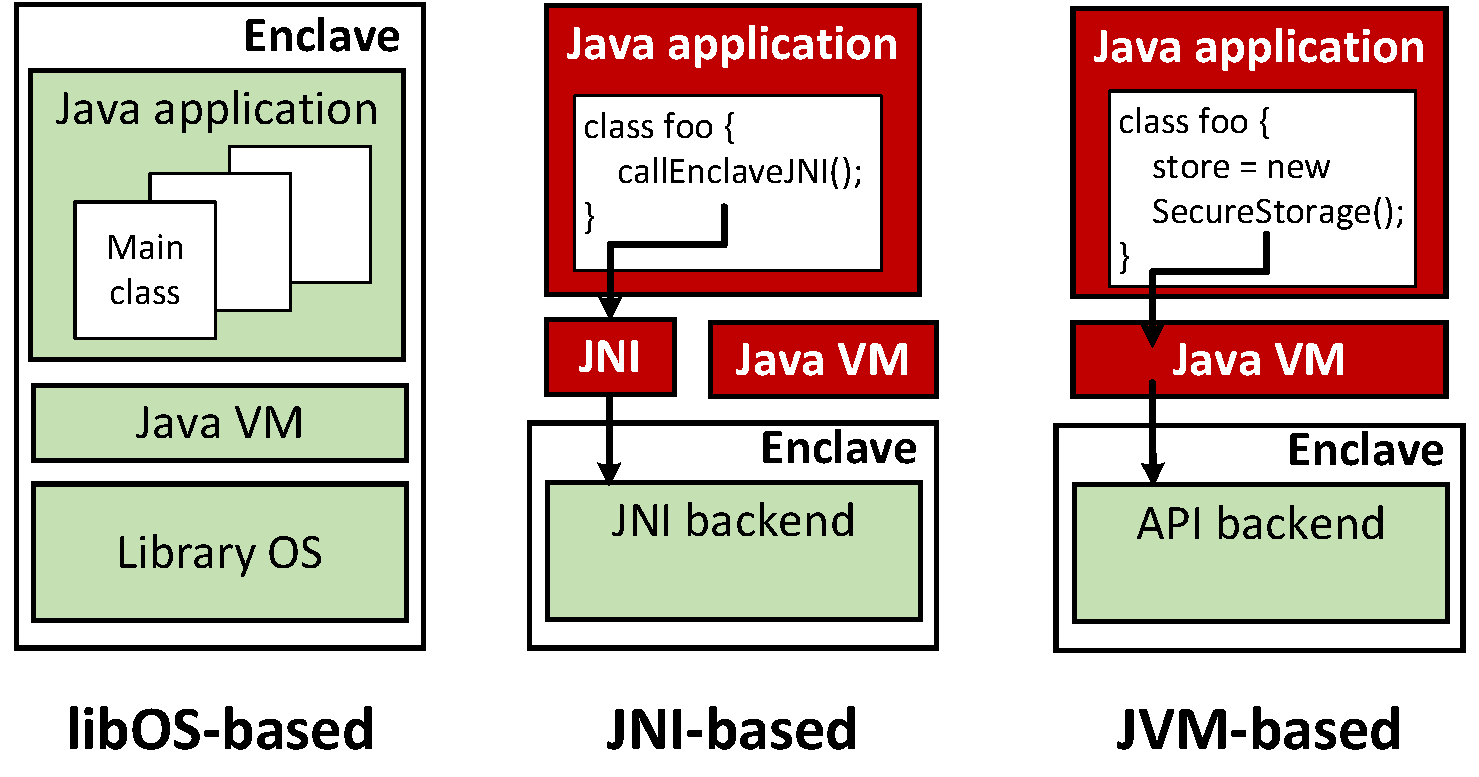
\includegraphics[width=\linewidth]{figures/alternatives.pdf}
\footnotesize
\caption{Alternative approaches to access \sgx{} hardware protection from \java{} applications.
The {\em \libos{}-based} approach runs the whole \java{} applications in the enclaves. 
The {\em JNI-based} approach uses JNI to run the security sensitive operations inside the enclaves.
The {\em \jvm{}-based} approach requires the \jvm{} to provide APIs to support common use cases of the enclaves.
Green (light) boxes are trusted components and red (dark) boxes are untrusted.
}
\label{fig:alternatives}
\end{figure}


Figure~\ref{fig:alternatives} illustrates the alternative approaches
to access \sgx{} hardware from \java{} applications:
The first approach is to run the whole \java{} applications with the \jvm{} inside the enclaves,
using a \libos{} ({\em \libos{}-based}).
This approach can secure applications as a whole,
but won't support any partitioned model for programming.
Another approach is to implement a JNI that create and interface with the enclaves
to run the security-sensitive operations ({\em JNI-based}).
The JNI-based approach is flexible enough for application developers
to implement the isolated components as well as the untrusted interface,
but requires developers to have the knowledge of
enclave implementation.
More importantly, the isolated components can only be developed in C or C++
language, so the applications lose the language protection of \java{} inside the enclaves.
A more plausible approach is to provide enclave-backed APIs
from the \jvm{},
to support common use cases ({\em \jvm{}-based})), such as a secure key-value store~\cite{vc3}.
Although the \jvm{}-based approach can save the application developers' effort
of implementing isolated components,
the use cases is limited to the pre-defined operations provided by the \jvm{} or the companion frameworks.
Because the backend implementation (isolated components and untrusted interfaces) in the \jvm{}-based approach is the same as the JNI-based approach,
the same language restriction also applies here. 

\end{comment}

%- Motivate the problem.
%- List all attack vectors
%- How can JAVA help?

\paragraph{Discussion}
Partitioning an application requires some input from the developer in order to identify 
sensitive data and code.  Each of the challenges above highlight cases where
Java either hides important information from the developer, or otherwise useful runtime
techniques can thwart the isolation benefits of using a hardware mechanism like \sgx{}.
A higher-level goal of \sysname{} is to provide constructs for the developer to specify
her goals, such as which objects should be isolated in an enclave,
and to have the language runtime use these developer-provided hints to 
make judicious choices on issues such as data placement.
A related goal is not eroding the benefits of developing in a high-level, managed language runtime.


%% The combination of language and hardware protections
%% is a technique used by many previous works.
%% However, the approach often seems like a trick of the trade for security experts:
%% the use of hardware protections is often deeply buried in the design of language protections,
%% as the underlying mechanism to bootstrap the trust
%% or to secure the core components of language protections.
%% %so that users (application developers) lose direct access
%% %to the security guarantees and features provided by the hardware.
%% %\fixmets{Think of an example: Maybe TPM.}
%% %The approaches of combining language and hardware protections are mostly ad-hoc to the use cases,
%% %i.e., how one protection is used to improve or reinforce another.
%% This work chooses a different approach,
%% by allowing \java{} applications
%% to straightforwardly utilize the protection of \sgx{} enclaves,
%% while still benefit from the safety properties
%% and advanced language protections from \java{}.
%% As a result, our framework also opens the win-win opportunity for
%% hardening both \sgx{} and \java{} protections.
%% \fixmedp{I also don't understand the point of this discussion.  What do you want the reader to learn from this?}

%\papersection{Threat Model}
\label{sec:threat}

In this section, we discuss the threat model of \sysname{},
including the adversaries,
and the components that must be trusted.

\paragraph{Adversaries}
We assume the same adversaries as other \sgx{} enclaves.
Any part of the system stacks, including the OSes,
device drivers, hypervisors, and even hardware,
such DRAM, GPU, buses, and peripheral devices, can be malicious
and attempt to attack the enclaves.
%The only trusted component is the CPU package, including L2 and L3 caches.
The attackers can perform any form of
online and offline attacks.
We also assume the attackers own all information
about \sgx{} hardware implementation, as well as every part of our solution.

We focus on the adversaries that target on
exploiting vulnerabilities in the isolated applications.
The attackers can manipulate any input to the application interfaces,
or the untrusted interfaces of the enclaves.
%Attackers may apply any techniques that compromise a regular privileged applications to compromise enclaves.
The vulnerabilities that attackers can exploit may not only fall in applications, but also in the infrastructures,
such as the libOS, the \java{} VM, JNIs and low-level interface to architecture.

%The only adversaries that are not addressed in \sysname{} are
%attackers exploiting {\em side channels} and
%{\em denial-of-service attacks}.
%Side channels, or even controlled channels, is a known problem of \sgx{} enclave
%and we expect to solve the problem in the future with
%stronger architectural support.
%Denial-of-service attacks are often considered benign for enclaves,
%because it only affect the ability of an untrusted host to legally access
%critical resources.

\paragraph{Trusted Components}
We trust any components loaded inside an enclave,
including the infrastructure (details discussed in Section~\ref{sec:implementation}), %(low-level interface, the libOS, \jvmname{}),
all supporting classes and their JNI,
and other resources or classes provisioned from remote hosts.
%All trusted components must be verified by either \sgx{} hardware or the infrastructure against their cryptographical measurements or checksums.
The implementation of \sgx{} hardware is also trusted to be invulnerable,
and use adversary-resistant key generators that cannot be compromised
by online or offline techniques.
We also assume \intel{} CPUs are resistant to direct, physical attack to the CPU packages, either to modify or peek into the chips.

\fixmets{Now JIT'ed code is not giving me error, but in case it fails later, we have to flip this discussion.}
We support running \java{} application both with and without JIT optimization.
Running \java{} application with JIT optimization
improve the performance of execution,
but can cause massive increase of the TCB of enclaves.
In case that JIT optimization is enabled in the enclaves,
the JIT compilers (\java{} VMs often have multiple JIT compilers, e.g., \jvmname{} has two) must be trusted by the users,
to always generate correct and invulnerable binary code.


%Note that in \sysname{} we disable JIT compiler that used to improve \java{} execution performance.
%The choice of disabling runtime compilation is due to the concerns that
%JIT compiler may largely extend the TCB because it must be trusted,
%and any bugs in different versions of compilers
%may causes code behaviors than what developers have tested and expect.
%Another practical reason is concerning the complexity and
%resources required for running a \java{} compiler with library OS in an %enclave.
%However, we consider these limitations to be not fundamental to the approach, and we keep compiler support in \sysname{} as a future work.



%In term of architecture, we trust the implementation of \sgx{} hardware,
%to maintain invulnerable implementation of \sgx{} instructions,
%and using adversary-resistant key generators that cannot be compromised
%by attacker using online or offline techniques.
%The CPU must keep enclave contents encrypted in DRAM and low-level caches that are shared by multiple cores.
%We also assume \intel{} CPUs are resistant to direct, physical attack to the CPU packages, either to modify or peek into the packages.

%\sysname{} protects confidentiality and integrity of provisioned security critical data in the trusted part of an application written in a high level managed language like JAVA.
% from the privileged operating system and the untrusted part of the same application. 
%\sysname{} assumes that the \sgx{} instructions are implemented correctly in the processor, and the SDK do not contain exploitable bugs to leak information. In addition, \sysname{} trusts the Graphene LibOS and the JVM running in the enclave with the trusted part of the application to not leak information. Thus, the security of the provisioned data is limited by the correctness of the processor, \sgx{}, Graphene LibOS, and JVM. \sysname{} also trusts the trusted part of the application to not leak information explicitly. \sysname{} prevents the trusted part of an application from implicitly leaking information.

%Threats that we do not cover
%\sysname{} inherits the threat model of \sgx{}~\cite{sgx}.
%The adversary controls the cloud provider's complete stack, OS, hypervisor, BIOS, system management mode, platform firmware, and device firmware. The adversary can also probe the memory and manipulate the I/O, but cannot read secret present in the processor.
%\sysname{} do not defend against attack vectors such as side-channel, covert-channel and control-channel~\cite{control-channel}. Denial of Service (DOS) attack is not part of \sysname's threat model. Even if the OS never schedules the enclave program or the untrusted part of the application is manipulated to never enter the enclave, no provisioned secret is leaked outside the enclave.


\chapter{System Overview}
\label{chap:overview}

\makeatletter
\def\input@path{{overview/}}
\makeatother
\graphicspath{{overview/figures/}}

%\section{Introduction}
%\label{sec:dcache:introduction}

Operating System kernels commonly cache file system data and metadata in 
a virtual file system (VFS) layer, which abstracts low-level file systems into a common API, 
such as POSIX.  
This caching layer has become a ubiquitous optimization
to hide access latency for 
persistent storage technologies, such as a local disk.
%whether a local disk or a network appliance, 
%have substantially higher access latencies than RAM,
%this caching layer 
%% SOSP Space - kind of quacking on
%% Caching
%% the file system directory hierarchy is particularly important because 
%% low-level file systems often spread this information across 
%% multiple disk sectors.
%% If an application wanted to open a single file on a system without a directory cache, 
%% most low-level file systems would issue numerous disk reads to locate the file and check the permissions
%% on the file and its parent directories;
%% a directory cache can commonly avoid these reads.
The directory cache is not exclusively a performance optimization; it also simplifies 
the implementation of {\tt mount}-ing multiple file systems, 
consistent file handle behavior,
and advanced security 
models, such as SELinux~\citep{selinux}.



%\fixmedp{Be charitable to developers, make our strong claims positively (we are really smarties) rather than calling them dummies}


%% Many observation shows that, in most systems, operations to storage are often
%% dominated by hierarchical structure traversal,
%% and fetching metadata of objects.\fixmetsai{references here}~\citep{duchamp94nfs}
%% In many file systems, traversal and metadata fetching
%% create random access patterns,
%% which are slower than sequential access patterns
%% on many storage media, e.g. magnetic disks.

% dp: I think this is getting down in the weeds.  We need to make the case for the work 
%     more strongly and generally first
%% Directory entry cache, a.k.a \dcache{},
%% is an important optimization in Linux kernels
%% to reduce storage operations for traversal and metadata fetching.
%% The design of \dcache{} is comparable to \vnode{} in BSD and \dnlc{} in Solaris.
%% \dcache{}, as well as \vnode{} and \dnlc{},
%% can be explained as a file system layer that
%% responds to requests on a cache hit,
%% but passes requests down to lower-leveled file systems on a cache miss~\citep{zadok06, skinner93}.

%\fixmedp{F1: Maybe thread together an argument about why no one would have tried a one-hop lookup before?}


%\marginpar{\scriptsize \textcolor{blue}{ Michael, I think the high-order bits are mostly right on Fig~\ref{fig:dcache:lookup-frac},
%but these number may change a bit as we refine the measurement}}

\begin{figure}[t]
\scriptsize
\centering
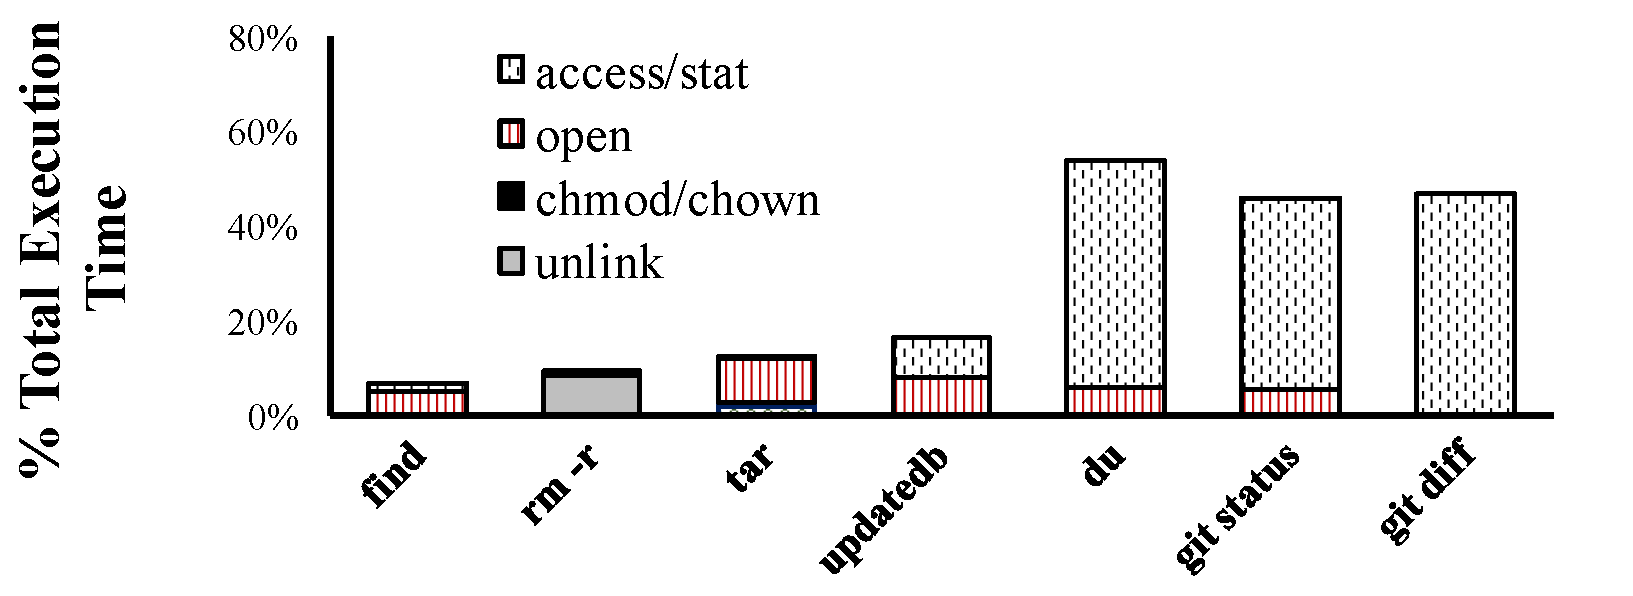
\includegraphics[width=5in]{dcache/plots/syscall-percentage.pdf} \\
\caption[Fraction of execution time on path-based system calls.]
{Fraction of execution time in several common utilities spent
executing path-based system calls with a warm cache, as measured with ftrace.}
\label{fig:dcache:lookup-frac}
%\vspace{-10pt}
\end{figure}

%\fixmedp{Please check these \% against time.  I think git diff is too high.  git status seems ok.}

Directory caches are essential for good application performance.
%Unix was designed such that ``(almost) everything is a file'',
%thus even accesses to in-memory file systems, device files, FIFOs and domain sockets
%first pass through the directory cache.
%In other words, 
Many common system calls must operate on file paths,
which require a directory cache lookup.
For instance, between 10--20\% of all system calls in the iBench system call traces do a path lookup~\citep{filenotafile}. 
Figure~\ref{fig:dcache:lookup-frac} lists the fraction of total execution time
%, as well as system time, 
several common command-line applications spend executing path-based system calls
(more details on these applications and the test machine in \S\ref{sec:dcache:eval}).
We note that these system calls include work other than path lookup,
and that these numbers include some instrumentation overhead;
% are coarse measurements that include  and work than path lookup;
%, and includes some time 
%for synchronous I/O (e.g., during {\tt rename}) as well as non-path tasks (e.g., creating 
%a file handle as part of {\tt open});
nonetheless, in all cases except {\tt rm},
the system call times and counts are dominated by
{\tt stat} and {\tt open}, for which 
%can be serviced from cache and for which 
path lookup is a significant component of execution time.
For these applications, path-based system calls account for 6--54\% of total execution time.
%and 25--77\% of system time.  
This implies that
lowering path lookup latency is
 one of the  biggest 
opportunities for a kernel to improve these applications' execution time.




\begin{figure}[t!]
\centering
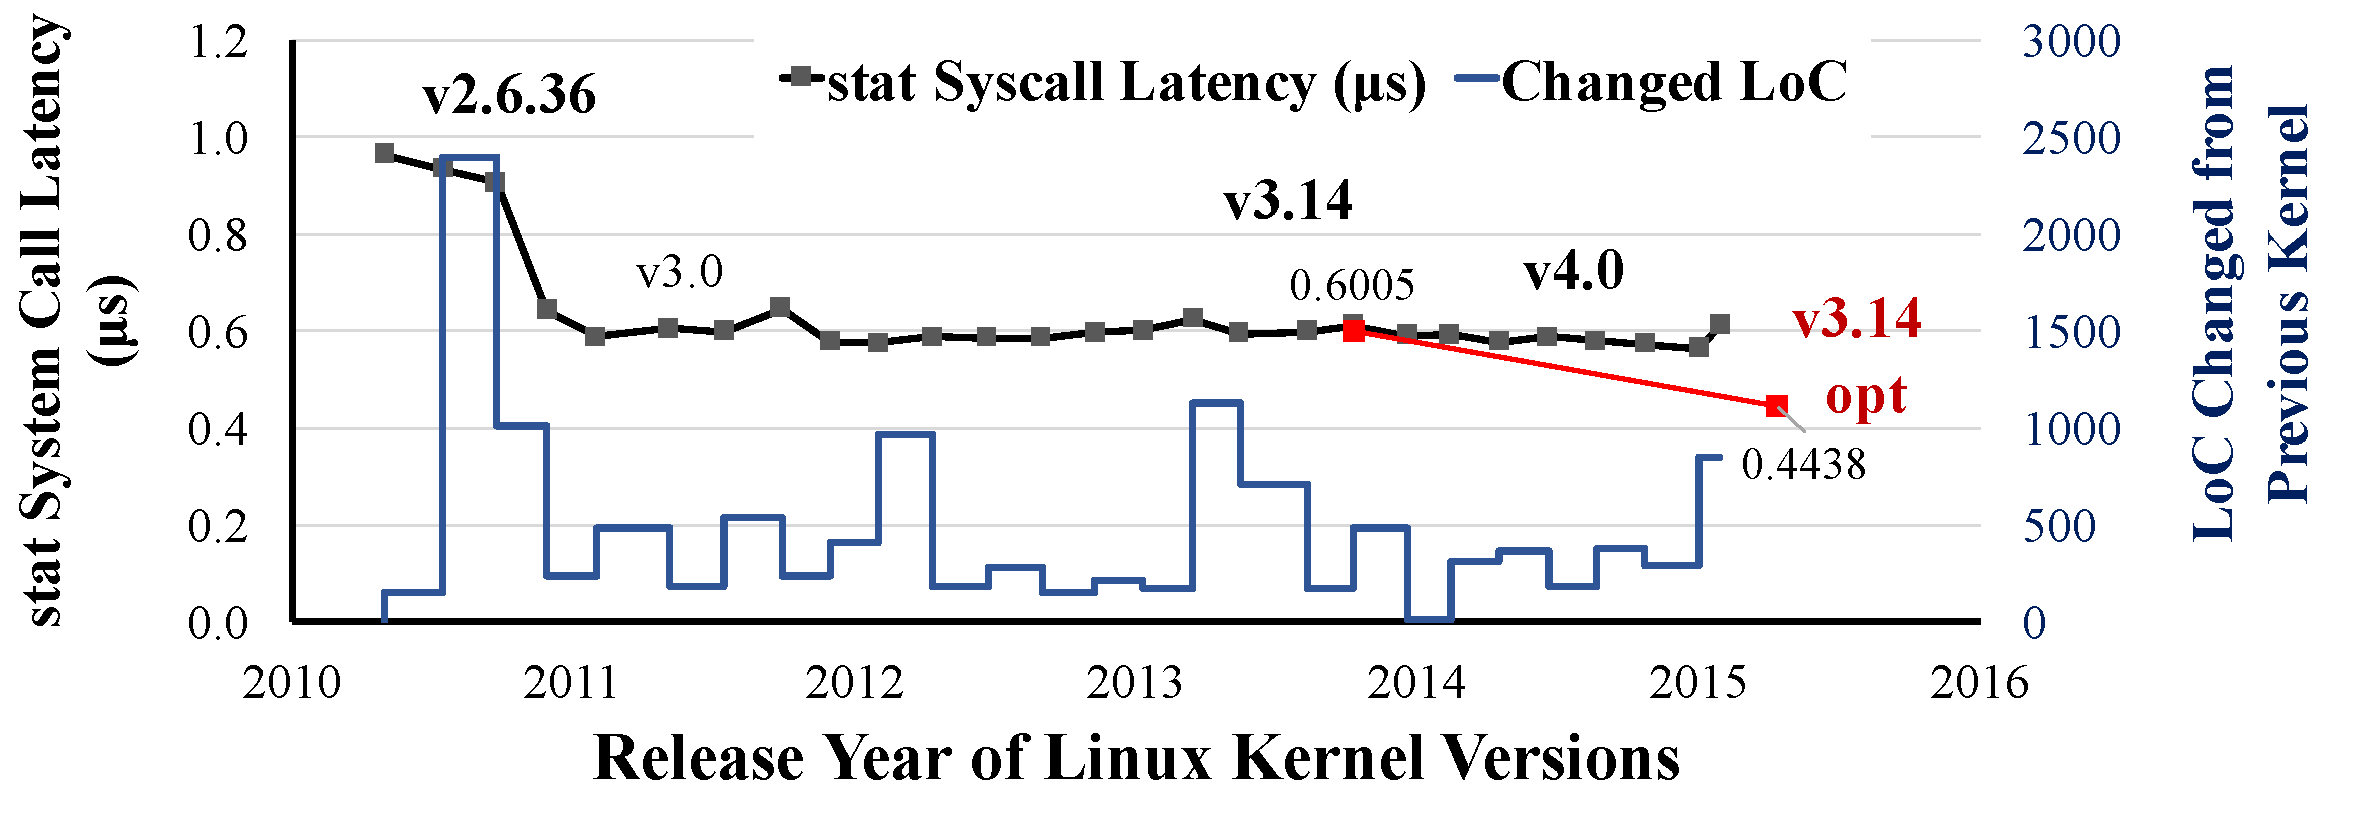
\includegraphics[width=6in]{dcache/plots/latency-by-version.pdf}
\footnotesize
\caption[Lantecy of {\tt stat} system call over years.]
{Latency of {\tt stat} system call with a long path {\tt XXX/YYY/ZZZ/AAA/BBB/CCC/DDD/FFF} on Linux over four years (lower is better), as well as the churn within the directory cache code (all insertions in {\tt dcache.c}, {\tt dcache.h}, {\tt namei.c}, {\tt namei.h} and {\tt namespace.c}). 
%Our optimizations significantly improve performance that has otherwise plateaued, despite significant ongoing developer effort.  
Our optimized \linuxver{} kernel 
further reduces {\tt stat} system call latency by \statspeedup{}\%.}
%\vspace{-15pt}
\label{fig:dcache:by-version}
\end{figure}


%\fixmedp{Add more evidence of lookup importance here: For instance, fraction of lookup time in file-related syscalls, or total lookup time in applications bound on file lookup latency.  }
Unfortunately, even directory cache hits are costly---0.3--1.1 \us{} for a {\tt stat} on our test Linux system, compared to only .04 $\mu$s for a {\tt getppid} and 0.3 \us{} for a 4 KB {\tt pread}. 
%\fixmetsai{Don, check this, I think read will be a better example, getppid is too trivial.}
This issue is taken particularly seriously in the Linux kernel community, which has 
made substantial revisions and increasingly elaborate optimizations to reduce the hit cost
of its directory cache, such as removing locks from the read path or replacing lock ordering with deadlock avoidance in a retry loop~\citep{corbet09jls,dcache-rcu}.
Figure~\ref{fig:dcache:by-version} plots directory cache hit latency against  lines of directory cache code changed 
over several versions of Linux, using a path-to-inode lookup \microbench{} on the test system described
in \S~\ref{sec:dcache:eval}.
These efforts have improved hit latency by 47\% from 2011 to 2013, but have plateaued
for the last three years.
%\fixmedp{if time, filter irrelevant changes from code deltas}
%at the cost of substantial developer effort.
%This latency appears to have plateaued 

The root of the problem is that the POSIX path permission semantics
seemingly require work that is linear in the number of path components,
and severely limit the kernel developer's implementation options.
%The root of this problem is that current directory cache
%designs reflect a straightforward implementation of the POSIX specification,
%which would seemingly require work that is linear in the number of path components.
For instance, in order to open file {\tt /\fnone{}/\fntwo{}/\fnthree{}} 
%for reading, 
one must have search permission
to parent directories {\tt /}, {\tt /\fnone{}}, and {\tt /\fnone{}/\fntwo{}},
as well as permission to access file {\tt \fnthree{}}.
The Linux implementation %of this specification is straightforward, 
simply walks the directory
tree top-down to check permissions.  
Unfortunately, when the critical path is dominated by 
walking a pointer-based data structure, 
including memory barriers on some architectures for multi-core consistency, 
modern CPUs end up stalling on hard-to-prefetch loads.
Moreover, because so many Linux features are built around this behavior, such as Linux Security Modules (LSMs)~\citep{wright+lsm},
namespaces, and mount aliases, it is not clear that any data-structural enhancements
are possible without breaking backward-compatibility with other Linux kernel features.
A priori, it is not obvious that a faster lookup algorithm, such as a single hash table lookup, 
can meet these API specifications and kernel-internal requirements; to our knowledge,
no one has tried previously.

%This paper proposes a decomposition of the directory cache, which allows
%most lookup operations to execute with a single hash table lookup (\S\ref{sec:dcache:dcache}),
%as well as optimizations to reduce the miss rate based on information that is {\em already in the cache}, but not used effectively (\S\ref{sec:dcache:readdir}).
%Our design maintains compatibility (\S\ref{sec:dcache:generalize}) through 
%several essential insights, including 
%how to separate the indexing of paths from checking parent permissions,
%and how to effectively and safely memoize the results of access control checks.


%% This paper proposes several new ways to organize a directory cache, which can yield 
%% substantial performance improvements over the current state of the art.
%% %This paper demonstrates that, despite this developer effort, there is still a substantial 
%% %missed opportunity hiding behind historical, intuitive, but not fundamental design choices.
%% Most of the Linux directory cache design reflects a straightforward implementation of the POSIX 
%% specification. %, with a division of labor that is suitable for mainstream file systems.

%This paper presents an alternative directory cache organization, which 
%improves performance by separating logical tasks, such as separating path indexing from permission checking; yet the design is sufficient to retain compatibility with POSIX.
%In the case of path lookup, 
%this paper demonstrates how 
%a per-component tree walk can be replaced with a single hash table lookup (\S\ref{sec:dcache:dcache}).
% without violating POSIX compliance.

%Our optimizations improve the performance of frequent lookup operations, but 
%introduce several costs, described in \S\ref{sec:dcache:dcache} and measured in \S\ref{sec:dcache:eval},
%which  we believe are acceptable and a net improvement for applications.
%First, these optimizations slow down infrequent modifications to the directory hierarchy, such as {\tt rename}, {\tt chmod},
% and {\tt chown} of a directory. 
%However, these slower operations
%account for less than .01\% of the system calls in the iBench traces~\citep{filenotafile}.
%Second,  the memory overheads of the dcache are increased.
%%(45\% per \dentry{}, as well as some  in our prototype).
%%(\fixmedp{XX MB} in our tests).  
%Third, lookup has a 
%probability of error from signature collisions that can be adjusted to be negligible
%%($2^{-141}$ in our configuration), 
%and within acceptable thresholds widely used by data deduplication systems~\citep{Debnath:2010:CSU:1855840.1855856, Srinivasan:2012:ILI:2208461.2208485, Quinlan:2002:VNA:645371.651321, Zhu:2008:ADB:1364813.1364831}.
%%, as well as how to remove
%%all memory barriers from the lookup path (\S\ref{sec:dcache:update}).
%In the micro-benchmark of Figure~\ref{fig:dcache:by-version}, our directory cache 
%optimizations improve lookup latency by 
%%revisions improve latency of accessing a long path
%%by 
%\statspeedup{}\% over unmodified Linux.
%%Our design addresses other missed
%%opportunities, such as identifying new opportunities to reduce the miss rate
%%through caching directory completeness.
%%\fixmedp{Do we want to highlight LoC?  3K is more than anything in the graph} \fixmetsai{Probably just mention in the evaluation. It's a metric that we should provide, but it's not awfully interesting.}
%%The total lines of code changed are fewer than 3,000 out of \fixmedp{XX}.
%%\fixmedp{Can we get 
%%, yet changes fewer than 3,000 lines of code.

%% SOSP cut - kind of long-winded
\begin{comment}
This paper rethinks current Linux directory cache design choices in light of the following goals:
\begin{compactitem}
\item {\bf Minimize the cost of a cache hit.} (\S\ref{sec:dcache:dcache}).
This means maximizing the benefit of temporal locality for frequent operations,
while pushing extra work of consistency maintenance onto less frequent, already-expensive operations.
%such as handling cache miss or updating massive metadata,
%in order to improve very frequent operations.
\item {\bf Maintain legacy compatibility.} (\S\ref{sec:dcache:generalize}).  Unix path semantics are complex, required by applications, file systems, and security modules, frustrating otherwise straightforward optimizations.  However tempting it may be to redesign path behavior to facilitate caching, path operations must exhibit the same behavior, with lower latency.
\item {\bf Never miss the same request twice in quick succession.} (\S\ref{sec:dcache:readdir}).  A number of less-frequent operations, such as reading a directory or secure temporary file creation, always miss in the cache {\em even if enough information is in cache to satisfy the operation.}  
%Of course, infrequent accesses should still be subject to a cache replacement policy, such as LRU.
\end{compactitem}
%Although directory caches must implement more complex semantics than a hardware memory cache,
%these principles should seem familiar to the reader with a basic architecture background.
%sadly, the Linux directory cache design violates all three.
\end{comment}

%This paper introduces several techniques to improve the performance of a directory cache,
%This paper explains several practical directory cache optimizations,
This paper demonstrates that these techniques improve performance for applications that use the directory cache heavily,
and the harm is minimal to applications that do not benefit.
%and that the worst case \microbench{} is only 12\% slower within \fixmedp{XX}\% of unmodified Linux.
%Each optimization we describe improves performance in isolation, and all can be combined.
%These optimizations change very few lines of code, and are backward-compatible with 
%legacy applications.  
%These changes are encapsulated in the VFS---individual file systems do not have to change their code.
%This paper describes a  prototype of these improvements implemented in Linux \linuxver{}.
%\S~\ref{sec:dcache:background} explains that the directory cache structure of Mac OS X, FreeBSD, and Solaris 
%are sufficiently similar that these principles should generalize.
%we compare and contrast Linux's directory cache
%with Mac OS X, FreeBSD, and Solaris in \S\ref{sec:dcache:background}, and explain inline how each
%optimization could be generalized to these other OS kernels.





%% \item {\bf Modularization and stackability}:
%% Any changes or optimizations must be implemented as modules inside Linux's VFS,
%% and can be stacked on top of the original design or any future optimizations. 
%% \item {\bf Backward compatibility}:
%% Any changes or optimizations must maintain least requirement of modifying any
%% file systems.
%% \item {\bf Generalization to other OSes}: Any changes or optimizations must be portable to other OSes with reasonable effort and change of design.




%% \dcache{} is proven to be effective on improving storage performance.
%% Experiments shows that,
%% in a Linux 3.x kernel, a \dcache{} with a xxx\% hit rate can speed up
%% metadata lookup and fetching time by xxx times.
%% \fixmetsai{experiment result, Linux version, and fs specs here}
%% However, we observed that Linux maintainers have made
%% constant and non-trivial efforts to improve \dcache{} in the Linux kernel.
%% We studied all \dcache{}-related source files in the Linux kernel Git repository,
%% and discovered that maintainers have committed
%% on average xxx revisions per source files.

%% We tested metadata lookup time on primary \dcache{}-related revisions.
%% Most changes on \dcache{} system only create xxx\%-xxx\% speed-up
%% than their predecessor.
%% \fixmetsai{result and graph here}.
%% Moreover, improvement to \dcache{} is still work-in-progress
%% for Linux maintainers.
%% \fixmetsai{reference to threads for latest dcache discussions}. 
%% All the evidences show that,
%% despite of significant reduction of storage operations,
%% efficiency of \dcache{} system internally still remains as a concern.

%% We argue that the design of \dcache{} needs to be carefully re-examined,
%% to fundamentally identify any missed opportunities that
%% improve value of \dcache{}.
%% At a high level, most optimization works for \dcache{} are focused on
%% improving ``how to cache'',
%% but we want to also lay eyes on ``what to cache'',
%% to ensure any valuable information returned from file systems
%% be captured by \dcache{} system.

%The contributions of this paper are as follows:
%\begin{compactitem}
%\item A performance analysis of the costs of path lookup and the opportunities
%to improve cache hit latency.
%\item A directory cache design that improves path lookup latency with a combination of techniques, including:
%  \begin{compactitem}
%  \item Indexing the directory cache by full path, reducing average-case lookup from linear to constant in the number of path components.
%  \item A Prefix Check Cache (PCC) that separates permission checking from path caching.  The PCC memoizes permission checks, and is compatible with LSMs~\citep{wright+lsm}.
%  \item Reducing the cost of checking for hash bucket collisions with path signatures.
%  \end{compactitem}
%\item Identifying opportunities to leverage metadata the kernel already has to reduce miss rates, such as tracking whether a directory is completely in cache.
%\item Carefully addressing numerous, subtle edge cases that would frustrate rote application of these techniques, such as integration with symbolic links and Linux namespaces.
%\item A thorough evaluation of these optimizations.  For instance, our optimizations improve throughput
%of the Dovecot IMAP server by up to \dovecotspeedup\% and latency of 
%updatedb by up to \updatedbspeedup{}\%.
%%git version control system by up to 25\%.
%
%\end{compactitem}

\papersection{\Thehostabi{}}
\label{sec:overview:host}

\issuedone{1.1.b}{Describe \thehostabi{} specification}
The development of \graphene{} starts with defining a simple host ABI (application binary interface) called \thehostabi{},
containing only OS abstractions essential to target applications.
%and is easily ported to different platforms.
%and minimal specifications for the host OSes and hardware.
%The host ABI is a new boundary between OSes (or hypervisors) and applications.
\Thehostabi{} separates
the implementation of an existing system API (application programming interfaces), which determines the compatibility against applications,
from hardware abstraction features, such as file systems, network stacks, and device drivers. 
\graphene{} moves the system API components
to a \libos{} in the userspace and reimplements the functionality using \thehostabi{}.
To port \graphene{} to a new host OS or hardware,
OS developers only have to implement \thehostabi{} on the target host system API,
%to new host OSes and hardware,
instead of paying a tremendous cost to translate the whole system API specification. Figure~\ref{fig:overview:porting} illustrates the porting process of \graphene{}.



%The host ABI separates the low-level, hardware management features, from the idiosyncrasy of system interface. 
%\graphene{} moves the upper layer of OS components,
%including the system calls and namespaces, into an library OS,
%leaving \thehostabi{} 
%as a narrowed interface to the host OSes and hardware.
%The host ABI intends to minimize the development effort on each host OS or hardware
%to mitigate the interface distinctions,
%to simply porting the OS abstractions defined in \thehostabi{}.


\begin{figure}[t!]
\centering
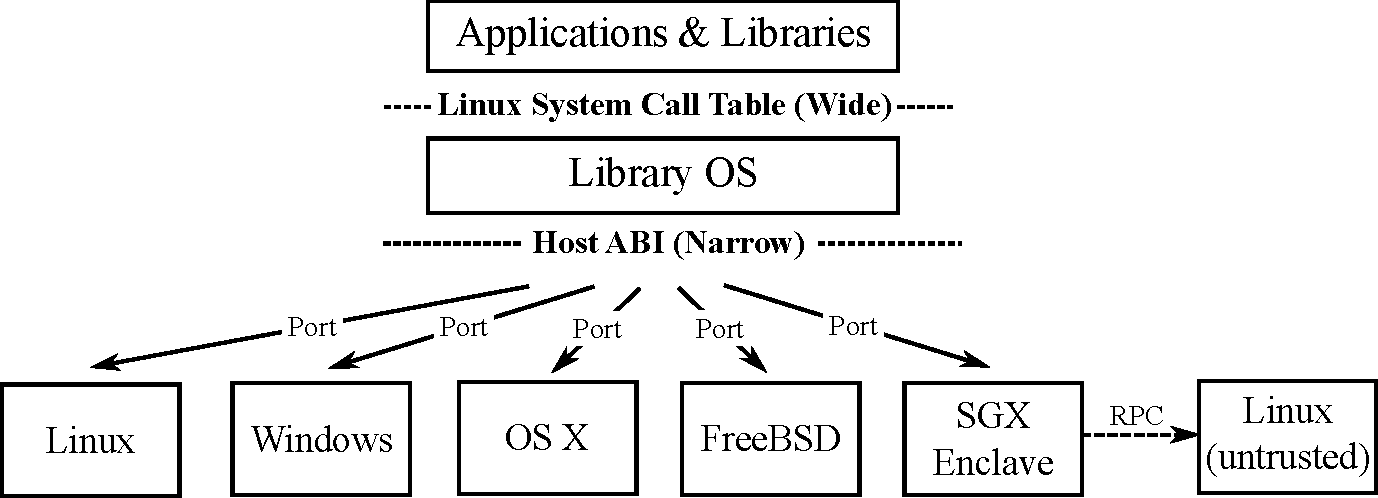
\includegraphics[width=30em]{porting.pdf}
\caption{Porting model of \graphene{}.}
%\vspace{-.1in}
\label{fig:overview:porting}
\end{figure}



\papersubsection{Platform Adaption Layers (PALs)}
\label{sec:overview:host:pal}


For each host OS or hardware, \graphene{} uses
a thin library called a {\bf platform translation layer (PAL)}
to translate among host interfaces.
%is loaded below the library OS, to translate each functions in \thehostabi{} to native system interfaces.
The main purpose of a PAL is to mitigate the semantic gap
between \thehostabi{} and
native host system APIs.
%The effort of PAL development is per host OS, whereas the library OS implementation is reusable on every hosts. %The simplicity of \thehostabi{} can be also estimated by the effort of implementing a PAL for each host.
By implementing a PAL on a new host OS or hardware,
users can reuse
the same \libos{} to run the same collection of unmodified Linux applications.
%To keep the porting effort low,
%the development of a PAL must be straightforward
%for average OS developers.
%to achieve with limited efforts.
%Based on the principle of porting simplicity, PAL development must be straightforward
%for average developers.







%The host ABI is defined for the simplicity of porting, as well as the sufficiency for implementing a library OS compatible to Linux.
%First of all, the number of host functions included in \thehostabi{}
%is much smaller than the number of system calls in a commodity OS such as Linux. 
\graphene{} currently contains PAL implementations for several popular OSes,
including Linux, \win{}, \osx{}, and FreeBSD.
%and \sgx{} with an untrusted Linux kernel.
Most of these OSes provide a POSIX-like system API similar to \thehostabi{}.
Due to the similarity, translating most of \thehostabi{} to one of the system APIs
are straightforward for average OS developers.
\Thehostabi{} is also much smaller than the actual POSIX API, making it extremely portable.



A part of \thehostabi{} may be challenging to port
on an OS,
due to unexpected system assumptions made by the OS.
For instance, \win{} does not support
fine-grained memory deallocation for de-privileged applications.
To implement system calls like \syscall{munmap} and \syscall{mprotect},
\graphene{} needs host ABIs to
deallocate or protect virtual memory pages at page granularity.
%A workaround is to change memory mappings at the physical page level,
%but will require running the \win{} PAL with root permissions.
%This type of porting challenges
%tends to be results of design decisions or assumptions made by OS developers.
%A \libos{} can potentially design
%different emulation strategies
%to compensate missing host abstractions.
A few host abstractions such as a bulk IPC feature are
optional to the host ABI;
if a host OS does not support these abstractions,
the \libos{} must fall back to alternatives. 

%In our experience, the development of a PAL is around ten thousand lines of code.

%For each port, the amount of code written for implementing \thehostabi{} is at the order of magnitude of thousands of lines of code, which is much more manageable than implementing a flat translation layer for system interfaces.


\begin{comment}
Based on the experience in \graphene{},
it is hard to ensure the portability of \thehostabi{} on every potential hosts.
%even a host ABI specialized for simplicity cannot guarantee to be portable on every hosts.
A host may simply lacks the functionality
for implementing a \hostapi{}.
The assumption is, maintaining the compatibility of \thehostabi{} poses a much less challenge than maintaining the whole system API.
Besides, the library OS may flexibly switch among emulation strategies
to compensate the absence of certain host abstraction.
As an example,
bulk IPC is optional in \thehostabi{} since its first definition,
due to the expectation
that implementing the feature may not be feasible on some hosts.
If bulk IPC is not available,
the library OS can fall back to RPC-based IPC, with a reasonable amount of performance penalty.
In the worst case, if there is no emulation strategies
to compensate for the absence of a \hostapi{},
user can predict the affected applications and avoid running these applications
on specific hosts. 
%at least users can predict whether an application will be affected and thus cannot run on certain hosts.
\end{comment}


%For a host OS that does not support ELF binaries, the PAL must follow the binary format which the host OS accepts, such as the Portable Executable (PE) format on \win{}.
%The PAL is the only layer in the user space which cannot be reused
%across different hosts. Besides the PAL, all of the other binaries in the user space are fully reusable, including the library OS, the supporting libraries, and the application executable.



%The host abstractions map to several common system calls in a commodity OS.
%For example, \funcname{StreamRead} and \funcname{StreamWrite} can directly map to the POSIX functions \funcname{pread} and \funcname{pwrite}, which are available in most OSes including Linux, BSD, \osx{}, and \win{}.
%More than half of the functions in \thehostabi{} can be counted toward this category.
%The rest of the host abstractions are either specific to Linux
%(e.g., TLS support),
%or belong to the POSIX functions that are not shared with commodity OSes
%(e.g., \funcname{mmap} on \win{}).
%The PAL emulates these host abstractions, using existing system interfaces available on the host OS, unless the software emulation is fundamentally impossible (e.g., restricted by the system interfaces), or too expensive (e.g., high overhead from copying data).



\papersubsection{Definitions and design principles}
 

\graphene{} defines \palcallnum{} calls in \thehostabi{} (also called \hostapis{}),
with a set of host abstractions
sufficient for \libos{} development.
%The host ABI defines the interaction between the library OS and a specific host.
%The \graphene{} library OS can be deployed on any ``host'' where \thehostabi{} has been ported.
This thesis defines
a {\bf host} of \thehostabi{}
to be an OS or hypervisor
which contains enough OS functionality for running a standalone application or virtual machine.
Most of the host targets in \graphene{}
are monolithic OSes,
including Linux, \win{}, \osx{}, and FreeBSD.
%which has defined a massive system API for programmability.
A monolithic OS 
usually contains a massive amount of system APIs,
which is sufficient for
implementing \thehostabi{}.


A special example of a host
is an \sgx{} (Software Guard Extensions) enclaves~\cite{intelsgx},
which
restricts OS functionality for security reasons.
The restrictions on \sgx{}
are results of a strong threat model
which distrusts any OS features except ones that are virtualized by the CPUs or migrated into enclaves.
The only way to obtain any missing OS features such as storage or networking
is to request through RPC (remote procedure call).
Requesting untrusted OS services through RPC also introduces new security threats that application developers tend not to anticipate~\cite{checkoway13iago,osdi16scone}.
Due to all the compatibility and security challenges discussed above,
this thesis uses \sgx{} as a representative example of a host
with unusual assumptions (e.g., threat models) and restrictions
compared to a monolithic OS.

%An innovative hardware abstraction like \sgx{} (software guard extensions)
%imposes unique assumptions and restrictions
%on a commodity OS,
%%creates a special host on top of Linux or \win{},
%%with unique interfaces and specifications regarding the host OSes.
%and thus creates a special host above the OS.

%If an OS has mutated or tweaked the interface for a hardware platform,
%such as an \sgx{} enclave 
%running on an untrusted Linux kernel,
%the combination of the OS (Linux) and the hardware platform (\sgx{}) is considered a specialized host.
%Especially, the \sgx{} port of \thehostabi{} faces several unique challenges,
%which will be discussed in Chapter~\ref{chap:sgx}.


\begin{comment}
%\fixme{each sentense should be a paragraph; starting the 2nd sentence}
\fixmedp{start with a strong opening stating the rationale}
The host ABI of \graphene{}
define functions needed from a host, in order to implement the library OS for reusing applications.
%to reuse an application and all its supporting libraries, including the \graphene{} library OS.
Each host of \graphene{} contains an OS and a hardware platform, either of which causes compatibility issues for running unmodified applications.
OS developers can port the library OS to a new host,
by simply reimplementing the narrowed host ABIs using abstractions available on the host.
%a new host platform.
%For each host which requires the compatibility for unmodified Linux applications, one only has to implement the narrowed host ABIs,
%instead of reimplementing the bloated, ``legacy'' system interfaces
%needed by the applications.
By implementing \thehostabi{}, OS developers skip the painful process of rebuilding the whole system interfaces of a commercial OS such as Linux.
The host ABIs strictly decouples the porting effort on the hosts from the compatibility feature for applications.
%The host ABIs decouple the OS development in the host and the implementation of compatibility for the existing Linux application.
What \thehostabi{} exposes is a simplified extended machine,
similar to a para-virtualization interface, capable of running the library OS as a lightweight virtual machine. % with compatibility against Linux applications.
%on which another layer of virtualization (i.e., the library OS) can be built to reproduce the compatibility for Linux.
\end{comment}


\begin{comment}
Two design principles drive the definition of \thehostabi{}s:
{\em simplicity} (i.e., easy to port on any hosts)
and {\em sufficiency} (i.e., containing enough OS functions for implementing a library OS).
The process of deciding \thehostabi{}s is comparable to
finding a ``pinch point'' within a OS implementation,
which can conveniently mediate a significant portion of OS execution paths for managing hardware abstractions.
%The two principles drive the development of \thehostabi{}s,
%The whole development of the \graphene{} library
%must be disciplined
%on extending \thehostabi{}s only when it is strongly required.
%of restraining extensions to \thehostabi{}s unless absolutely necessary.
The two principles
determine the soundness of the \graphene{} approach to improving compatibility
for any hosts.
\end{comment}


%%The host ABI is defined with partitioning in mind.
%\Thehostabi{} 
%determines a boundary which partitions several upper-level OS components, %, such as system calls and namespaces,
%into a library OS,
%%, as a dynamically-linked library which can be deployed
%%to various hosts.
%%The rationale behind the partitioning is based on the fact that not every OS component is equally important to compatibility, for applications which need to be ported across hosts.
%%When an OS is extended for a new hardware,
%%these OS components usually remain unchanged, or are predominantly reused.
%%Partitioning
%%into a library OS further guards these 
%in order to isolate the host idiosyncrasy. % on specific hardware. %any potential changes for adopting new hardware.
%%Similar isolation
%%exists in traditional OSes, but without partitioning:
%The strategy
%is also used in OSes:
%An example is the Linux virtual file system (VFS), an internal interface
%which encapsulates operations of file system drivers.
%%On the other hand,
%%drivers (e.g., drivers for file systems, block devices, or network cards)
%%and architecture-specific instructions
%%stay encapsulated in the host OS.
%%in the Linux kernels are usually encapsulated under a virtualized, in-kernel interface (e.g., the Linux virtual file system),
%%to simplify the development of the rest of the kernel.
%Similar to VFS,
%\thehostabi{} is intended
%to be a more ubiquitous interface,
%which encapsulates
%any host-specific behavior and semantic
%inside the host OS.
%%for encapsulating both OS and hardware idiosyncrasy on a wide range on hosts.
%%declares a ubiquitous system interface, to encapsulate both OS and hardware abstractions
%%for the library OS.




\Thehostabi{} shares several characteristics with a virtual hardware interface
exported by a hypervisor.
A generic, backward-compatible
virtual hardware interface
%a set of generic, virtual hardware,
%which the VM can control with the same drivers.
allows an unmodified OS kernel to run inside a virtual machine as on the bare metal.
%by exporting interfaces close to commodity hardware.
%To avoid additional porting effort, the virtual hardware are close to the typical commodity hardware.
%For instance, a virtual hardware interface
%usually includes a virtual NIC (network interface controller),
%such as the virtualized E1000 interfaces
%available in VMware workstation or QEMU.
%As a result, \thehostabi{} contains the
%typical OS features and interfaces, similar to the API of early UNIX systems.
The key difference between
a virtual hardware interface
and \thehostabi{}
is that \thehostabi{} does not target reusing a whole, unmodified OS kernel as a guest.
Instead, 
\thehostabi{} contains higher-level abstractions such as files and network sockets
to ensure portability on most host OSes.
The concept
of defining \thehostabi{}
with a customized guest OS (i.e., a \libos{}) running atop \thehostabi{} is similar to para-virtualization.
%\thehostabi{} expects the \libos{}
%to be rewritten and
%customized for \thehostabi{},
%similar to a 
%para-virtualizated VM.
%Compared to an actual para-virtualized VM,
A para-virtualized VM defines hypercalls as interfaces between a guest OS and a hypervisor.
Furthermore, \thehostabi{} avoids duplication of OS components
such as scheduler, page fault handler, file systems, and network stacks
between the host and \libos{}.
%Another difference is that \thehostabi{} is called by normal function calls, whereas para-virtualization relies on hypercalls.
To compare a VM and a \libos{} on a spectrum,
a VM reuses a whole OS on a wide, backward-compatible virtual hardware interface
whereas a \libos{} implements only system API components on a simplified host ABI.

The following paragraphs discuss the key design principles of \thehostabi{},
including porting simplicity, sufficiency for \libos{} development, and ease of migration.

\paragraph{Porting simplicity.}
%To reduce porting effort
%\thehostabi{}
%must be simple to port on a host OS or hardware.
To reduce porting efforts,
\graphene{} defines \thehostabi{}
using two strategies:
first, \graphene{} significantly reduces both the size and complexity of host OS features
that OS developers have to implement.
Effectively, \graphene{} avoids duplicated OS features and handling rare corner cases
on \thehostabi{}.
%The development of \graphene{} disciplinarily avoiding adding any functions to \thehostabi{},
%unless the library OS cannot internally implement an OS feature.
Second, the definition of \thehostabi{}
imitates common system APIs in a POSIX-like monolithic OS,
to directly translate most calls to
a few similar host abstractions.
%existing system calls or system library functions
%on each host.
%include functions which can be directly mapped to OS functions exported by the host.
%%the likelihood of finding similar features on the host, to be translated to functions in \thehostabi{}.
%The assumption that such a strategy is possible
%is based on
%the observation that
%%similarity of system interfaces is common among most OSes.
%similar OS functions, especially UNIX-style APIs,
%tend to commonly exist in most OSes.
%, to reduce the learning curve for programming applications.
For instance,
the stream APIs in \thehostabi{}, such as \palcall{StreamRead} and \palcall{StreamWrite}
are similar to
system calls like \syscall{read} and \syscall{write} exist on Linux, BSD, and POSIX API,
or \syscall{ReadFile} and \syscall{WriteFile}
on \win{}.
%with similar functionality and semantics.
%and 
%looks similar to \syscall{ReadFile} in \win{}, except the data types.
%The definition of \thehostabi{}
%is based on observations of the system interfaces in some of the important hosts,
%including Linux system calls and \win{} API.
%exported by the targeted hosts,
%and defines the functions in \thehostabi{}, to be easily translated to the native system interfaces.
%The host ABI is essentially a subset of the common features from every potential hosts.
%We expect %\thehostabi{} defined with simplicity in mind
%to be straightforward to port on most hosts,
%Most functions in \thehostabi{} can be easily translated to host system interfaces
%in various styles.
As the rest of this thesis proves, porting \thehostabi{} is straightforward
on most monolithic OSes.

%For example, \thehostabi{} defines \syscall{StreamRead} and \syscall{StreamWrite} for accessing I/O streams, similar to .
%xcept some nuanced details like order of parameters.


% by including OS functions , such as \syscall{FileRead} and \syscall{FileWrite}, similar to the Linux system calls, \syscall{pread} and \syscall{pwrite}.




\begin{comment}
The simplicity of \thehostabi{}s requires retaining a minimalist design of host functions. %, based on typical OS services for managing hardware.
%\graphene{} reduces the host functions
%to the bare minimum.
The host ABIs should only contain operations that
are absolutely necessary for requesting external hardware abstractions.
%A way to simplify \thehostabi{}s is to move host functions into the library OS
%and to replace them with wrappers consisting of other host functions.
Any functions that can be partially or wholly implemented inside the library OS
should be further simplified, or even removed from \thehostabi{}s.
%---in other words, whether \thehostabi{}s can be further reduced.
Moreover, \thehostabi{}s have to be simple enough to implement on
most hosts;
%In the simplest host ABIs, none of the host functions shall be able to internally implement the behavior of another host function,
%or the definition of \thehostabi{}s is further reducible.
that is, \thehostabi{}s should contain only OS functions that are commonly offered on
most hosts.
The host ABIs are close to simplified UNIX interfaces,
such as reading or writing a file or an I/O device as a byte stream,
or creating a virtual memory mapping.
%the most common OS functions
%offered on most of the potential hosts,
For most hosts,
implementing \thehostabi{} should be as straightforward as redirecting the functions to the closest host system calls.
%such as the Linux system calls or the \win{} APIs.
For example, the functionality of \syscall{StreamRead} and \syscall{StreamWrite} in \thehostabi{}s can loosely match with
\syscall{read} and \syscall{write} in Linux,
or \syscall{ReadFile} and \syscall{WriteFile} in \win{}.
%This thesis also evaluates the simplicity of \thehostabi{}s by counting the lines of code used to implement \thehostabi{}s on each host platforms.
Since most OSes have inherited a similar design from UNIX,
it is fair to assume finding
comparable OS functions %host platforms
to \thehostabi{} would be reasonably easy.
%fair to assume that \thehostabi{}s 
\end{comment}



\paragraph{Sufficiency for \libos{} development.}
%\Thehostabi{} defines
%the host abstraction available for a \libos{} to access host hardware abstractions.
To develop a \libos{} with compatibility against a wide range of applications,
\thehostabi{}
%are demonstrated by the fact that
%the exported host functions 
contain any OS abstractions that the \libos{} cannot easily emulate.
%and a full-function library OS is implemented on top of them.
For most hosts,
the host OS abstractions
%can be categorized into five types:
include
process creation, memory management, and I/O (typically, files and network connection)~\cite{dhamdhere2007os-textbook}.
%Besides security and protection,
%the definition of \thehostabi{} is closely related with hardware management,
%and offers the most basic abstractions for each category of OS functions.
%managing specific types of hardware,
%and each contain a few basic abstractions
%which can be expanded into other system interfaces.
%For example, the basic OS functions for memory management include
%allocating (\syscall{VirtMemAlloc}),
%protecting (\syscall{VirtMemProt}),
%and deallocating (\syscall{VirtMemFree}) memory regions. % at certain granularity
%(usually in pages).
%These basic functions can be used to implement other forms of memory allocation,
%such as growing heaps with \syscall{brk}
%or allocating thread-private stacks.
%The definition of the \drawbridge{} host ABI is a hint, for creating a list of host abstractions necessary for the library OS, including streams, memory, threads, and processes. 
%If \thehostabi{}s are insufficient for implementing certain system interfaces, one may extend \thehostabi{}s with the missing functions,
%with the discipline to retain the simplicity of \thehostabi{}s.
%The extension to \thehostabi{}s must be d, to keep the extension minimal, and to avoid adding redundant functions.
%The implementation of the \graphene{} library OS demonstrates that
%\thehostabi{} is sufficient for implementing significant portion of Linux system calls.
For each type of abstractions,
a monolithic OS may define several variants of system APIs with similar functionality.
For instance, Linux provides two system calls, \syscall{mmap} and \syscall{brk}, both for memory allocation in a process.
\syscall{mmap} allocates larger memory regions with page granularity,
whereas \syscall{brk} simply grows a single, continuous heap space for more fine-grained allocation.
Many applications such as GCC~\cite{gcc}
switch among system API variants in case one of them is unavailable on certain OS distributions.
This thesis shows that,
by adopting only the semantics of one of these similar APIs or abstractions, the host OS can stay simple with
the \libos{} emulating the rest of APIs.
For instance, \thehostabi{} includes \syscall{VirtMemAlloc}
as a similar feature as \syscall{mmap},
which is sufficient to emulating both \syscall{mmap} and \syscall{brk}.



\graphene{} defines \thehostabi{} partially based on
\drawbridge{},
a library OS for single-process \win{} applications.
The host ABI of \drawbridge{} 
contains 36 functions,
%demonstrates that its host ABI is sufficient
%for running a library OS in which 99.7\% of code comes from the \win{} 7 source.
%The host ABIs of \drawbridge{} are later extended
%for running a Linux-based library OS called Bascule~\cite{baumann13bascule}.
and several works have ported the host ABI to different hosts,
including \win{}, Linux, Barrelfish, and \sgx{}~\cite{porter11drawbridge,baumann14haven,mssql-on-linux,baumann13bascule}.
%and is capable of running a library OS for single-process, Linux applications, with a few host ABI changes~\cite{baumann13bascule}.
%ill loads and links the rest of application binaries, just like the native Linux loader (i.e., \code{ld.so}).
%\graphene{} takes the high-level definitions of the \drawbridge{} and Bascule host ABIs, and customizes for general-purpose Linux applications and a wider range of hosts. 
Although running \win{} and Linux applications may face
a different set of challenges,
the nature of their APIs is mostly similar, with a few exceptions.
During the development of \graphene{}, developers found the occasions in which
the host ABI of \drawbridge{}
is not sufficient to address Linux-specific challenges
and decide to extend \thehostabi{}.
Section~\ref{sec:overview:host:abi} and Chapter~\ref{chap:abi}
will further discuss the Linux-specific extensions of \thehostabi{}.


\paragraph{Migration.}
The \graphene{} library OS shares several features of VMs, including checkpointing and migrating a running application.
Migrating a process is also the key to emulating copy-on-write forking,
on a host without physical memory sharing (e.g., \sgx{}).
A hypervisor checkpoints and migrates a VM by snapshotting the VM states above a stateless virtual hardware interface. % as a clean boundary for snapshotting the application and OS state.
\Thehostabi{} is also defined to be statelessness,
by ensuring any states in the hosts to be temporary and reproducible to the applications and \libos{}.





\papersubsection{The \hostapis{}}
\label{sec:overview:host:abi}


%\fixmedp{the beginning doesn't capture the whole paragraph.}
%The host ABI shares several common abstractions with production OSes.
%The functions in \thehostabi{}
%define the basic features needed from the hosts, to run the library OS.
%The definition of the host functions
%should be unsurprising to average OS developers,
%making the implementation on a new host to be fairly straightforward.
%The host ABI reflects the common functionality of most OSes, including Linux and \win{}.
%Although the same OS abstractions may be defined
%as different idiosyncratic system interfaces on each host OSes,
%\graphene{} takes into consideration of porting the host functions to either OSes, in the most effortless way possible.





%fixmedp{give more of the background}
Table~\ref{tab:overview:abi} lists the \palcallnum{} calls defined in \thehostabi{}:
%Among these \hostapis{}, 
25 calls are inherited from the \drawbridge{} host ABI,
including functions to managing I/O (e.g., \palcall{StreamOpen}), memory allocation (e.g., \palcall{VirtMemAlloc}), scheduling (e.g., \palcall{ThreadCreate}), and several miscellaneous functions (e.g., \palcall{SystemTimeQuery}).
%Most of the host functions only affect the OS or hardware states
%related to the process itself.
%For example, \syscall{VirtMemAlloc} can only allocate memory in the calling process,
%and cannot affect other processes running in parallel.
%Only I/O streaming functions export states to the host OS, and share states with other processes or library OSes.
14 calls are added by \graphene{}, to implement Linux-specific features.
For example, unlike \win{} or \osx{}, Linux %The host ABI is also complemented with several Linux-specific abstractions, such as
delivers hardware exceptions to a process as signals.
Linux also requires 
the x86-specific segment registers (i.e., FS/GS registers)
to determine the location of thread-local storage (TLS), which can be hard-coded in application binaries by a compilation mode of GCC.
On \win{} or \osx{}, the x86-specific segment registers are mostly ignored, and even frequently reset to eliminate attack vectors.
%The host ABI contains host functions (), which can be directly called from the library OS. \graphene{} shows that \thehostabi{} is sufficient to implementing a large portion of the Linux system calls.
%These functions are not defined in \drawbridge{}, the \win{}-based library OS,
%because these abstractions do not exist in \win{}.
%The \drawbridge{} host ABI does not contain exception delivery because the feature is
%not commonly used in \win{} applications.
%Moreover, the x86 segment registers cannot be modified in \win{}
%because the OS assigns fixed values to these registers
%for the whole execution.
%Although \drawbridge{} excludes these abstractions, Bascule extends \thehostabi{} to include similar functions,
%demonstrating that the extension is indeed necessary.
\graphene{} discovers these abstractions as a necessity for implementing a rich Linux \libos{}.



\begin{table}[htp!]
\centering
\input{abi-table}
\caption{An overview of \thehostabi{} of \graphene{}. The ones marked with the symbol $\dagger$ are introduced in the initial publication of \graphene{}~\cite{tsai14graphene} or later extended for this thesis. The rest are inherited from \drawbridge{}~\cite{porter11drawbridge}.}
\label{tab:overview:abi}
\end{table}

%The interfaces, as part of \thehostabi{}, which access these host abstractions, are ultimately simplified to reduce the porting effort on each host.
%Unlike the system interfaces in the OS, \thehostabi{} does not prioritize backward compatibility. Therefore, \thehostabi{} includes only the minimum interfaces that the library OS needs to interact with the host. The host ABI does not have to include any of  the legacy system interfaces from a production OS, let alone preserving different flavors of system interfaces for backward compatibility.



\graphene{} introduces five calls for 
remote procedure call (RPC) between \libos{} instances
in a multi-process application.
\graphene{} simplifies porting multi-process abstractions
on each host OS
to implementing RPCs.
The basic RPC abstraction is 
a pipe-like RPC stream for message passing between processes.
To improve performance,
%RPC is critical for implementing the coordination of OS states
%across library OS instances.
%The basic form of RPC in \graphene{} is a pipe-like RPC byte stream, which a library OS can simply use to send messages.
%It is a common design choice
%to implement inter-process coordination through message-passing
%instead of shared memory, especially for hardware platforms that do not guarantee memory coherence~\cite{baumann09barrelfish}.
%A problem to the message-passing approach is the significant overheads
%on frequently exchanging distributed OS states.
\thehostabi{} defines an optional, bulk IPC abstraction
to send large chunks of virtual memory
across processes.
%The bulk IPC feature works similarly as sending the memory through RPC streams,
%but is much faster because it avoids copying memory in the host.


%for host platforms that urgently require lowering the RPC overheads.
%Another extension is for
%%\funcname{StreamSendHandle} and \funcname{StreamRecvHandle}
%delegating opened stream handles to another process, through a connecting pipe.
%The feature is similar to sending file descriptors
%through UNIX sockets in Linux, and is used to share opened network sockets with the \syscall{fork}'ed processes.
%%Another RPC abstraction is a bulk IPC channel; a process can use \funcname{PhsyicalMemoryCommit} to commit a large chunk of memory to a bulk IPC channel, which \funcname{PhsyicalMemoryMap} can map into another process, as copy-on-write. The library OS uses bulk IPC as an optimization to \syscall{fork}.
%Despite that either of the RPC primitives
%is not necessary easy to implement on every hosts, the inclusion of these host functions is completely optional, and the library OS can always fall back to the message-passing approach.



%All the host functions are designed to appear as ``stateless''
%as possible to the library OS.
%Being stateless to the library OS means that
%a host function does not preserve any permanent state of certain host abstraction.
%A stateless function can recover
%from disconnection of the library OS, and be reconnected at any timing.
%The host functions can maintain temporary bookkeeping for the convenience of porting,
%but should not assume the bookkeeping states to be permanent.
%The principle of defining all the host functions to be stateless
%is primarily for two purposes:
%{\em migration} and {\em security isolation}.
%For migration, the fact that the library OS can disconnect freely from the host functions simplifies the implementation of the migration feature.
%Migration is also an important foundation to implementing \syscall{fork}, because the cloned process need to receive a snapshot of the parent process.
%For security isolation, 
%a stateless host function is easier to check,
%because the security monitor only has to verify each instance of host function calls,
%instead of tracing multiple host functions over a longer period of time.

%the functions to access each host abstraction must appear \fixmedp{clarify `stateless'} stateless to the host, except for the handles to identify the resources. Each call to the host functions is independent. The arguments given for each call must be always be absolute values, instead of relative values.
%For example, the offset given to \funcname{StreamMap}, \funcname{StreamRead}, and \funcname{StreamWrite} (if the opened handle is a file) are offsets from the beginning of the file, and thus are irrelevant to how many bytes that are previously written or read.
%When enforcing isolation rules, the host OS can check the arguments of each calls to the host functions, independently and atomically.


%A host ABI (application binary interface) has to define the convention of application binaries, including the binary format and the linking procedure, as well as a set of  system interfaces.
%The host ABIs contain a minimal loader which recognizes a basic version of the ELF (Executable and Linkable Format), just enough to compose a binary of the library OS.
%The very initial loading procedure as part of \thehostabi{}s only loads a clean library OS instance.
%Each host of \graphene{} is supposed implement a minimal dynamic loader,
%which can load the \graphene{} library OS binary in ELF.
%The library OS then completes the dynamic loading procedure,
%by directly loading the Linux native dynamic loader (i.e., \code{ld.so}), and indirectly loading the rest of the application binaries.







\papersubsection{Host-enforced security isolation}
\label{sec:overview:host:security}


To target multi-tenant environments, 
\graphene{} enforces strong security isolation between mutually-untrusting applications running on the same host.
The security isolation of \graphene{} is comparable to running each application
in a VM or a container.
Just as a virtual hardware interface isolating each VM,
\thehostabi{} also enforces security isolation between library OS instances.
%according to the trust model of the applications.


On a trusted host OS,
\graphene{} delegates security isolation as a host-level feature.
The library OS and the application must mutually trust each other, due to lack of internal privilege separation in a process.
%The host ABI also separates API implementation
%from security isolation.
%To ensure isolation, each host must restrict access from the applications or the library OS, to any unauthorized host abstractions.
On each host, a reference monitor enforces security isolation policies, by access control on OS abstractions sharable among processes, including files, network sockets, and RPC streams.
%The host-level security isolation is orthogonal to API complexity.
Separating security isolation from API implementation simplifies security checks
for applications that only require
complete protection from other tenants.
%based on monitoring the references to host resources and rejecting authorized resource access.
%to the host abstractions.





%\graphene{} reduces the attack surface exposed to applications
%by restricting access to the host kernel ABI 
%and prevents access to unauthorized system calls, files, byte streams,
%and network addresses with a \emph{reference monitor}.
%The host kernel ABI exported by the \pal{} heavily 
%limits the ability of a \graphene{} application to interact with the rest of the system;
%any external interactions are further mediated by a reference monitor.
%Unlike a typical Linux system, \graphene{} applications cannot interact with shared 
%system daemons or other shared system resources.
%As a result, \graphene{} enforces security isolation similar to running applications in separate VMs---even
%applications that span multiple processes.


In \graphene{},
one or multiple processes of the same application run in a {\bf sandbox}.
Multiple library OS instances coordinate
in a sandbox
to present a unified OS view
to the application.
%As the library OS instances can coordinate shared OS states using simple RPC streams,
The design simplifies the enforcement of security isolation for multi-process abstractions.
\graphene{}
uses the reference monitor to block RPC streams across the sandbox boundary,
stopping applications in different sandboxes from accessing multi-process OS states.
%\graphene{} contributes a multi-process security model 
%based on the abstraction of a \emph{sandbox},
%or a set of mutually trusting processes.
%If a reference monitor exists, the reference monitor permits the processes within the same sandbox to communicate and exchange RPC messages, but disallows cross-sandbox communication.
The current design focuses on security isolation, although we do expect to extend the design for more sophisticated policies
in the future.

\begin{comment}
The only host abstractions that are shared across processes and must be mediated by the host for isolation are files, network sockets, and RPC streams
--- all other allowed host ABI modify only local process state, such as VMAs and threads.
%Thus, the reference monitor need only mediate file access, socket and RPC stream creation.
%an unprivileged daemon
%as well as extensions to the App\-Armor LSM~\cite{apparmor},
%which checks file and socket policies in the kernel.
%, reducing context switching overhead
%and the risk of race conditions~\cite{garfinkel03traps}.
In order for the reference monitor to restrict file access, socket and RPC stream creation,
each application includes a {\em manifest file}~\cite{hunt07rethink},
which describes a {\tt chroot}-like, restricted view of the local 
file system (similar to Plan 9's unioned file system views~\cite{pike90plan9}),
%including read-only shared files,
as well as {\em iptables}-style~\cite{iptablesman} network firewall rules.
To facilitate sharing read-only libraries, a manifest may specify a file system view which combines several different sub-directories of the local file system, and can prevent writing to files or directories.


For example, the \graphene{} reference monitor on the Linux host is implemented using \syscall{ioctl} to a special device (\code{/dev/graphene})~\fixme{a prospective design}.
A process is restricted by the Linux BPF-style system call filter, or the SECCOMP filter~\cite{seccomp}, to use \syscall{open} to access any files, or to \syscall{connect} or \syscall{bind} to any sockets.
It must use the \graphene{} special device to open or create streams, so the file paths or network addresses can be checked against the sandbox rules. The kernel module as the driver of the \graphene{} special device can coexist with any Linux Security Module (LSM), such as AppArmor~\cite{apparmor} or SELinux~\cite{selinux}.


When a new process is launched by the host, it begins execution in a new sandbox.  
Child processes may either inherit their parent's sandbox, or can be started in a separate sandbox---specified by a flag to the host abstractions of process creation.
A parent may specify a subset of its own file system view 
when creating a child, but may not request access to new regions of the host file system. 
%The restrictive policy enforced on the child will be written in a new manifest file generated by the parent, and the policy will be checked by the reference monitor.
The child may also issue an {\tt ioctl} call to 
dynamically detach from the parent's sandbox. The reference monitor prevents byte stream creation across sandboxes.
%among picoprocesses
%that are not in the same sandbox.
%and restricts external connections to remote URIs according to firewall rules in the manifest.
When a process detaches from a sandbox, effectively splitting the sandbox, the host must closes all RPC streams that could bridge the two sandboxes.
\end{comment}



\paragraph{Threat model.}
For most hosts, application trusts the host OSes as well a \libos{} instances in the same processes.
For multiple processes inside a sandbox,
the \liboses{} in these processes
also trust each other.
Applications or \liboses{} are not trusted by the host OSes or processes outside of the sandboxes.
Applications and \liboses{}
can become the adversary to the host OS,
by exploiting vulnerabilities on \thehostabi{}.
%the \graphene{} design reduces the attack surface between the hosts and the library OS instances, to defend against a malicious application.

%On a host with a reference monitor, the host OS and the reference monitor are both trusted, to mediate all system interfaces used to implement \thehostabi{}. The host must check all access to any abstractions with effects outside of a process's internal state, such as an opened file, or a connected network socket.
%Processes inside the same sandbox mutually trust each other. The adversary can run arbitrary code inside of one or more processes within one or more sandboxes.
%The adversary can control all code in its processes, including the library OS and the host-specific PAL.
%{\tt libLinux} and the \pal{}. 
%We also assume a trusted reference monitor process running on the host kernel that 
%launches \graphene{} applications and mediates all system calls with external effects,\fixmedp{define precisely}

%\graphene{} ensures that %The key security property the \graphene{} design upholds is that 
%the adversary cannot interfere with any victim picoprocesses
%in a separate sandbox.  
%The \graphene{} sandbox design ensures strict isolation: 
%if the only shared kernel abstractions are byte streams and files, 
%and the reference monitor ensures
%there is no writable intersection between sandboxes,
%the adversary cannot interfere with any victim picoprocess.


The threat model of \graphene{} on \sgx{}
contains the adversary from other hosts but excludes
the host OS, hypervisor, and any hardware except the CPU from its trusted computing base (TCB).
An untrusted OS or hypervisor
potentially has lots of opportunities to invade applications or VMs,
using Iago attacks~\cite{checkoway13iago}.
The challenges of porting \graphene{} to \sgx{} is not limited to resolving the compatibility issues of enclaves but also defending applications and \liboses{} against untrusted host OSes.







%%% The only processes allowed to run as standard kernel processes (non-\graphene{}) 
%%% are the reference monitor and
%%% system administration utilities that need more kernel interfaces than the \pal{} ABI provides.
%%% Ensuring that a collaborating picoprocess correctly implements
%%% some function (such as receiving a signal),
%%% as well as preventing exploitation of vulnerabilities in picoprocesses
%%% are beyond the scope of this work.

%\graphene{} reduces the system attack surface of the host, but does not change the size of its
%trusted computing base; however, reducing the effective system call table
%size of a picoprocess does facilitate adoption of a smaller host kernel,
%which we leave for future work.


\papersection{The \libos{}}
\label{sec:overview:libos}

This section gives the overview of \graphene{}, a library OS for reusing unmodified Linux applications
on \thehostabi{}.
%Existing library OSes have established reuse of single-process applications~\cite{porter11drawbridge}.
%The library OSes map a target system API, such as the Linux system calls, to abstractions in \thehostabi{}. %The reduction of host interfaces provides portability to various platforms that can translate the interfaces to host APIs or abstractions,
%and a narrower attack surface that developers can more likely reason about.
% and supporting data structures as library functions---mapping
%high-level APIs onto
%a few paravirtual interfaces to the host kernel.
%Recent library OSes improve efficiency over full guest OSes by eliminating duplicated features
%between the guest and host kernel,
%such as the CPU scheduler, or
%eliminating guest-level multiplexing code, as the library OS supports only one application;
%even compiling out unnecessary guest kernel APIs~\cite{unikernels}.
A \libos{} is comparable to a partial, guest OS running in a virtual machine.
However, compared with an actual virtual machine, the \libos{} design of \graphene{} and previous work~\cite{porter11drawbridge,unikernels} eliminates duplicated features between the guest to the host kernel, such as the CPU scheduler or file system drivers, and thus reduces the memory footprint.
%Library OSes have also been proven useful for reusing applications on new hardware platforms, such as \sgx{} enclaves~\cite{baumann14haven}.
%% dp: This sentence seems a little premature
%In recent works, library OSes provide rich OS features for isolated contexts while the host OSes are untrusted

%% Library OSes reduce the memory requirements of running a self-contained,
%% isolated application process
%% %guest \daniela{I would replaced guest by "isolated process or group of processes (a \libos{} instance)''}
%% by orders of magnitude
%% In a cloud computing environment,
%% increasing the number of applications per server has enormous
%% economic benefits.
%% Even on a desktop or portable system, \libos{}es can reduce the overheads
%% of sandboxing untrusted code and running applications
%% designed for another OS.

%Because library OSes execute within a VM \daniela{this phrase does not read good to me because (i) it might imply the picoprocesses need hypervisor support, as misunderstood by reviewer 1 and (ii) you already emphasized the drawbacks of leveraging a VM} or lightweight process ({\em picoprocess}~\cite{xax}),
%library OSes execute with

%% dp: Daniela, great suggestion!  We need to make this situation seem more
%%     like the sky will fall without our help
A principal drawback for prior library OSes is the inability to support multi-process applications. Many existing applications, such as network servers (e.g., Apache) and shell scripts (e.g., GNU makefiles), create multiple processes for performance scalability, fault isolation, and programmer convenience.
%These applications would benefit from the efficiency and security benefits
%of a library OS.
For the efficiency benefits of library OSes to be widely applicable,
especially for unmodified Unix applications,
library OSes must provide commonly-used multi-process abstractions, such as \syscall{fork}, signals, System V IPC message queues and semaphores, sharing file descriptors, and exit notification.
Without sharing memory across processes, the library OS instances must coordinate shared OS states to support multi-process abstractions.
%To support multi-process abstractions, library OSes often have to rely on sharing OS states,
%backed by the hosts' memory sharing features.
For example, \drawbridge{}~\cite{porter11drawbridge} cannot simulate process forking because copy-on-write memory sharing is not a universal OS feature.


\begin{figure}[t!]
\centering
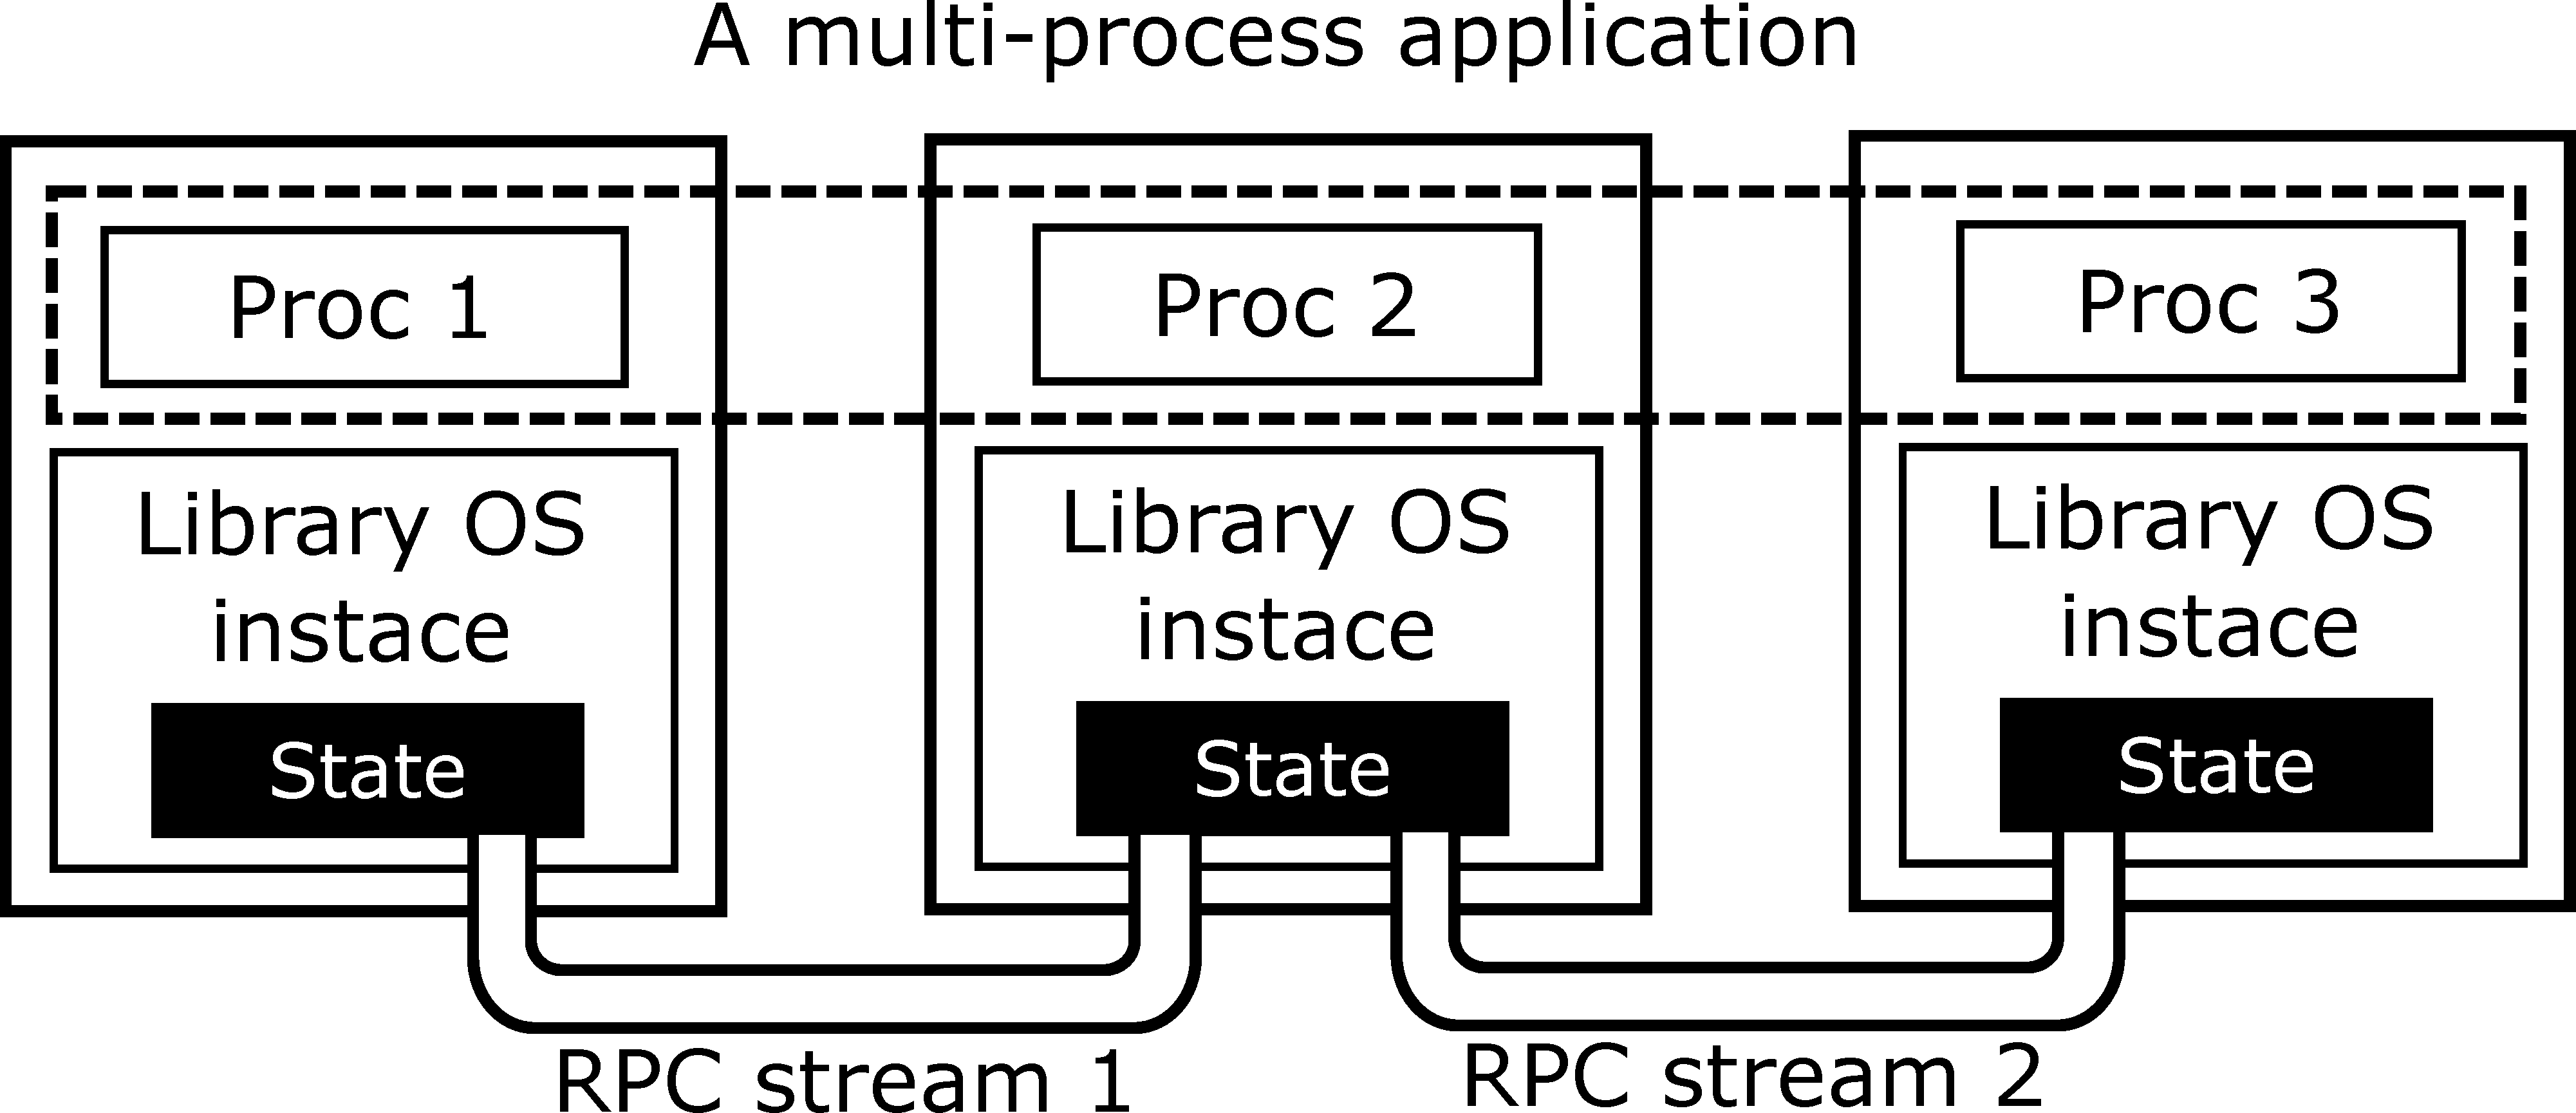
\includegraphics[width=24em]{concept.pdf}
\caption{Multi-process support model of \graphene{} \libos{}. For each process of an application, a \libos{} instance will serve system calls and keep local OS states. States of multi-process abstractions are shared by coordinating over host-provided RPC streams, creating an illusion of running in single OS for the application.}
%\vspace{-.1in}
\label{fig:graphene:concept}
\end{figure}

%{\bf \graphene{}} is a Linux-compatible library OS to run legacy, unmodified Linux applications. 
In \graphene{}, multiple library OS instances collaboratively implement
Linux abstractions, but present single, shared OS view to the application.
\graphene{} instances coordinate states
using message passing over RPC streams.
With a distributed POSIX implementation,
%placement of shared state and messaging complexity are first-order performance concerns.
%%We chose to shift implementation complexity into the library OS
%%in order to uphold simple enforcement of security isolation in the host.
%By coordinating shared states across library OS instances, 
\graphene{} can create an illusion of running in a single OS for multiple processes in an application.

%Previous library OS designs ensured security isolation of independent applications,
%comparable to a VM, by keeping a relatively narrow host ABI.
%We selected the \graphene{}
%design because it strikes a unique balance between
%and robust, flexible security enforcement.
%The \graphene{} design ensures security isolation of
%mutually distrusting, multi-process
%applications on the same host system.
%Essential to this goal is
%minimally expanding the host ABI to support multi-processing,
%as well as leveraging RPCs as a natural point to mediate inter-\picoproc{} communication.
%RPC coordination among \graphene{} instances can be dynamically disconnected, facilitating novel sandboxing
%techniques.  For instance, we develop an Apache web server extension that, upon logging in a given user,
%places the worker process's \libos{} in a sandbox with access to only that user's data.
%We expect more nuanced degrees of trust are possible in future work.

%\graphene{}'s design gives the user and system administrator a high degree of flexibility
%in isolating arbitrary groups of unmodified application processes,
%while upholding the efficiency and host compatibility benefits of recent library OSes.

%\fixmedp{After a complete draft is written, coalesce all goals and make sure they are addressed early on.  We are doing some scatter-shot motivation}


\papersubsection{\Libos{} architecture}
\label{sec:overview:libos:arch}

%Recent library OSes~\cite{porter11drawbridge,unikernels,baumann13bascule,osv}
%are designed for security and efficiency, but are limited to single-process applications.
%The security isolation of \liboses{} derives from 
%limited, explicit data sharing and 
%a narrow host interface.  
A \libos{} typically executes in either a para-virtualized VM~\cite{unikernels,osv}
% \daniela{I would have the use of a VM as a discussion topic in the end of the paper.}, 
or an OS process called a \emph{\picoproc{}}~\cite{porter11drawbridge,baumann13bascule}, with a restricted host ABI.
%The host ABI heavily restrict effects outside of the application's address space
%as a result, applications in a \picoproc{} have very little opportunity to interfere with each other,
%yielding security isolation comparable to a VM.
%The library OS deduplicates features for hardware management in both the guest and host kernels.
\graphene{} executes within a \picoproc{} (Figure~\ref{fig:overview:arch}),
which includes an unmodified application and its supporting libraries, which run alongside a library OS instance.
The \graphene{} \libos{} is implemented over \thehostabi{} designed to expose very generic abstractions that are easy to port on any host OS.
%Although the \graphene{} prototype  host kernel is Linux, 
%we adapt a host ABI from Drawbridge/Bascule,
%which has been previously implemented on \win{}, Hyper-V, and Barrelfish~\cite{porter11drawbridge,baumann13bascule,baumann09barrelfish}.
%The \graphene{} host ABI is
% summarized in Table~\ref{tab:abi} and discussed in more detail in \S\ref{sec:linux:pal}\fixmedp{if not cut...}.  
%which exposes only tens of simple host calls. \daniela{briefly define \picoproc{}: A \picoproc{} is unmodified application code running with a \libos{}.}


\begin{figure}[t]
\centering
\begin{minipage}[b]{1.25in}
\footnotesize
\raggedleft
Linux system calls \\
\graphenesyscallnum{} out of \linuxsyscallnum{}\\
\vspace{0.1in}
Host ABI \\
\palcallnum{} \hostapis{}\\
\vspace{0.2in}
\hostsyscallnum{} Linux system calls
\vspace{0.35in}
\end{minipage}
\hspace{-1.25in}
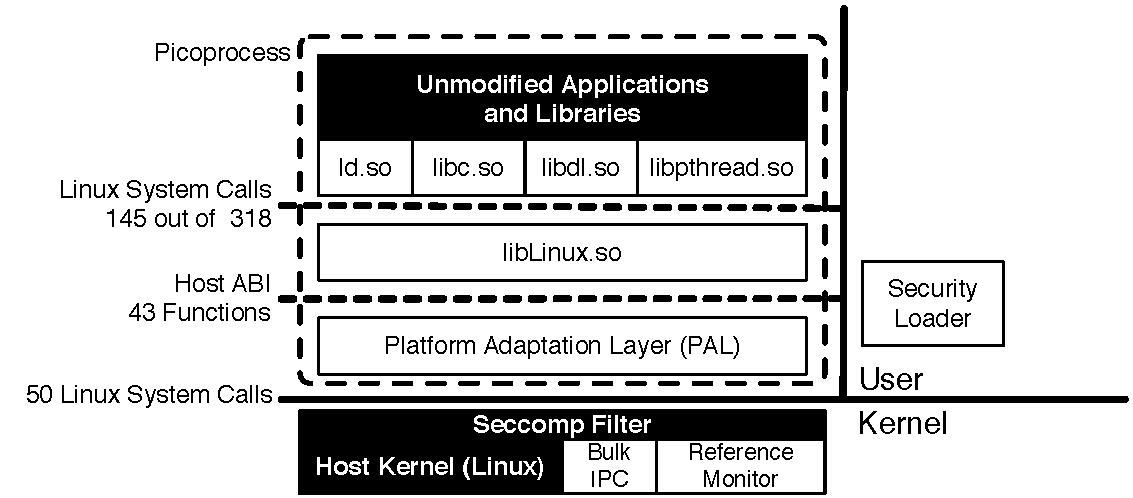
\includegraphics[width=32em]{arch.pdf}
\caption{Building blocks of \graphene{}.  Black components are unmodified.
We modify the four lowest application libraries on Linux:
{\tt ld.so} (the ELF linker and loader),
{\tt libdl.so} (the dynamic library linker),
{\tt libc.so} (standard library C),
and {\tt libpthread.so} (standard threading library), that issue Linux system calls as function calls directly to {\tt libLinux.so}.
Graphene implements the Linux system calls using a variant of the Drawbridge ABI, which is provided by the platform adaption layer (PAL).
A trusted reference monitor that ensures \libos{} isolation is implemented as a kernel module. Another small module is added for fast bulk IPC, but it is optional for hosts other than Linux.}
\label{fig:overview:arch}
\end{figure}


%\graphene{} shows the sufficiency of \thehostabi{} to support a rich Linux \libos{}.
As an example of this layering, consider the heap memory management abstraction. Linux provides applications with a data segment---a legacy abstraction dating back to original UNIX and the era of segmented memory. The primary thread's stack is at one end of the data segment, and the heap is at another.  The heap grows up (extended by \syscall{brk}) while the stack grows down until they meet in the middle.
In contrast, the host ABI provides only minimal abstractions for allocating, deallocating, and protecting regions of virtual memory.
This clean division of labor encapsulates idiosyncratic abstractions
in the library OS.


%These interfaces are host-independent \daniela{OS or kernel-independent}, as they tend to be very generic and easily
%implemented on any host OS kernel or VMM \daniela{postpone VMM for later}.

At a high level, a \libos{}
scoops the layer just below the system call table out of the OS kernel
and refactors the code as an application library.  
The driving insight is that there is a natural, functionally-narrow division point 
one layer below the system call table
in most OS kernels.
Unlike many OS interfaces, \thehostabi{} minimizes the amount of application state in the kernel, facilitating
migration. A \libos{} instance can programmatically read and modify its OS state, copy the state to another instance, and the remote instance can 
load a copy of this state into the OS---analogous to hardware registers.
A \picoproc{} may not modify another \picoprocs{}' OS states.



\papersubsection{Multi-process abstractions}
\label{sec:overview:libos:multiproc}


\issuedone{1.3.b}{An overview of multi-process support}
A key design feature of UNIX is that users compose simple utilities to create more significant applications.  Thus, it is unsurprising that many popular applications are multi-process---an essential feature missing from previous \liboses{}.
%This gap is filled by the \graphene{} \libos{}, which
%extends recent \liboses{} to support multi-process applications.
The underlying design challenge is minimally expanding a tightly-drawn isolation boundary without also exposing idiosyncratic kernel abstractions or re-duplicating mechanisms in both the host kernel and the library OS.

%requires a careful balance among the competing goals of 
%efficiency, host independence, and security isolation.
%The challenge, then, is minimal expansion of

%\vspace{5pt}
%\noindent {\bf Motivating Example.~}
For example, consider the process identifier (PID) namespace. In current, single-process library OSes, \syscall{getpid} could just return a fixed value to each application.
This single-process design is isolated, but the library OS cannot run a shell script, which requires forking and executing multiple binaries, signaling, waiting, and other PID-based abstractions.

%\paragraph{Design options.}
%Multi-process support requires extensions to the host ABI of recent, single-process library OS designs. Because multi-process abstractions, such as signals or System V IPC, tend to be idiosyncratic, an essential problem is identifying a minimal, host-independent substrate upon which  to implement OS-specific abstractions.
There are two primary design options for multi-process abstractions in \liboses{}: (1) implement processes and scheduling in 
the library OS; (2) treat each library OS instance as a process and distribute the shared POSIX implementation across a collection of library OSes.
\graphene{} follows the second option, which imposes fewer host assumptions.
%, maximize flexibility in mapping processes to physical resources, and facilitate inter-process security policy enforcement. % as enforcing security policies on related processes.

Multi-process abstractions
inside the library OS also possibly benefit from
hardware MMU virtualization, similar to
the model explored by Dune~\cite{belay12dune}.
However, this design reintroduces a duplicate scheduler and memory management.
Moreover, Intel and AMD have similar, but mutually incompatible MMU virtualization support,
which would complicate live migration across platforms.
None of these problems are insurmountable, and it would be interesting in future
work to compare both options.


In \graphene{}, multiple \liboses{} in multiple picoprocesses collaborate to implement shared abstractions. \graphene{} supports a rich of Linux multi-process abstractions including copy-on-write forking, \syscall{execve}, signals, exit notification, and System V IPC semaphores and message queues.
For instance, when process A signals process B on \graphene{}, A's library OS instance issues a query to B's instance over a pipe-like
RPC stream, and B's instance then calls the appropriate signal handler.
The host OS is unaware of the implementation
of multi-process abstractions,
as well as security isolation of the corresponding states.

%%% All collaborating \libos{} instances exchange messages as needed 
%%% to provide the application with a consistent view of 
%%% shared abstractions,
%%% such as


%\graphene{} approaches multi-processing by selectively replicating state and issuing remote procedure calls (RPCs) 
%%across multiple, collaborating
%library OS instances.
%Guests may work together to provide the unmodified multi-process application with
%coordination abstractions 

%%Shared abstractions on \graphene{}'s are implemented outside of the host, ensuring  host OS independence.
%% by implementing these
%%shared abstractions entirely
%%outside of the host kernel.
%%Shared abstractions are implemented outside of the host.
%%From the host kernel's perspective, 
%\graphene{} implements all shared abstractions by cooperatively managing the abstraction states over RPC streams.
%Single-process applications still service system calls from local state, and \graphene{}, includes optimizations to place state where it is most likely to be used, minimizing RPC overheads.
%The host reference monitor can easily isolate picoprocesses by 
%% \graphene{} design isolates \liboses{} by 
%%requiring all coordination to use 
%%explicit bytes streams \daniela{, pipe-like abstractions provided by the kernel. (suggestion: Reviewer  3)}.
%%Security isolation is enforced
%%by a kernel-level {\em reference monitor}, which can 
%%disconnect or prevent creation of a
%blocking all RPC messages, % between \liboses{} that should be isolated,
%without the need to understand the library OS details or semantics of these abstractions.
%In the PID example, only mutually-trusting picoprocesses can signal each other.
%%if the reference monitor prevents creation of RPC streams
%%across mutually untrusting \picoprocs{},
%%the \liboses{} cannot exchange signals.

%%% \graphene{} is designed to 
%%% The \graphene{} design leverages a number of optimizations to service application system calls 
%%% from local state whenever possible, and to minimize message passing overheads otherwise
%%%  (\S\ref{sec:namespaces:insights}).
%%% Our experience is that starting with a local system call design and then extending it to share state is relatively straightforward,
%%% and introduces little-to-no overhead when the request can be serviced locally.


The \graphene{} library OS is also capable of gracefully handling disconnection from other library OSes, facilitating dynamic application sandboxing.
RPC streams may disconnect at any time by either the reference monitor or at the request of a library OS.
%Message streams may be severed externally, by the reference monitor, or 
%one guest may simply disconnect from others to isolate itself.
%An application may disconnect itself from the 
%Any \graphene{} application may dynamically detach from the confederation, 
%or a host-level sandbox may dynamically separate two guests by severing their communication channels.
When a picoprocess is disconnected, the library OS will handle the subsequent
divergence, %and the library OS will will fork these abstractions
{\em transparently} to the application.
For instance, if a child process disconnect RPC streams from the parent by the reference monitor, the library OS will interpret the event as if the other process terminated, close any open pipes, and deliver exit notifications.
% \daniela{(applications run unmodified) - Reviewer 1 asked clarification on transparently}.

%% A key insight behind our design is that the common use case for these \daniela{cooperating} abstractions
%% is between a pair of processes.  Thus \graphene{} leverages a number of optimizations 
%% to reduce broadcast messages, avoid replication of needless state,
%% and service requests locally


\paragraph{Comparison with microkernels.}
The building blocks of \graphene{} are very similar to the system abstractions of a 
microkernel~\cite{liedtke95sosp,klein09sel4,elphinstone13microkernels,liedtke93sosp,chen93memory,baron1985mach-1,accetta86mach}, except a microkernel often has an even narrower, more restricted interface than the host ABI.
%such as the port and
%message abstractions of Mach~\cite{
A multi-server microkernel system, such as GNU Hurd~\cite{hurd} or Mach-US~\cite{stevenson95mach-us}, implements Unix abstractions across a set of daemons that are shared by all processes in the system. \graphene{}, on the other hand, implements system abstractions as a library in the application's address space and coordinates library state among \picoprocs{} to implement shared abstractions. \graphene{} guarantees isolation equivalent to running 
an application on a dedicated VM; it is similar to implementing the security isolation model on a multi-server microkernel by running a dedicated set of service daemons for each application.

%%% \graphene{}'s differences are motivated by two considerations: efficient support of both stand-alone, 
%%% single-process applications and multi-process applications; as well as flexible security isolation. 
%%% \graphene{} contributes techniques to seamlessly and efficiently transition 
%%% between single-process and multi-process support, as well as adapting 
%%% some known techniques to a new environment.

%The \graphene{} host ABI could be described as a hybrid microkernel, which also exposes the file system and network of the host kernel.
%Similarly, picoprocesses are assumed to be provided by a production OS, like Linux or \win{}, or by a Type 2 hypervisor.  A bare metal hypervisor could potentially export a PAL, but would require services from a trusted VM, such as Xen's dom0~\cite{barham03xen}.
%%or the \pal{} would implement more thread scheduling, networking, and file system code;
%%or the \pal{} ABI would change to push this code into the \libos{}.
%Arguably, recent library OS designs might be improved by rethinking the division of labor, but this is beyond the scope of this thesis.

%\paragraph{Alternatives.}
%Another approach to support multi-process applications in a library OS would be to use hardware MMU virtualization such as nested paging used by a system like Dune~\cite{belay12dune}
%in order to implement a second process abstraction, memory manager, and scheduler in the library OS.
%This approach threatens the efficiency benefits of deduplicating these features.
%A final option is exposing additional system interfaces, such as signals, by adding more system calls to a picoprocess. This approach undermines compatibility, as many of these coordination abstractions tend to be very OS-specific.
%%Unix signals vs.\ \win{} events, {\tt waitpid()} vs.\ blocking on a process handle, etc.
%%Although legacy OSes do enforce some access control rules on coordination abstractions,
%%kernel developers must audit and add hooks to millions of lines of code.
%%As a result,
%%users have lost confidence that a traditional OS can comprehensively enforce 
%%security isolation on these abstractions---a key motivation for using VMs
%%for security isolation.


%Systems must strike a careful balance between the competing goals of
%security isolation and multi-process coordination.
%Multi-process applications require OS-managed coordination abstractions such as signals, process exit notification, and System V IPC.
%These coordination abstractions operate within shared namespaces, such as the process ID namespace and the System V key space.
%These coordination APIs and namespaces must be consistent among coordinating processes, but can undermine security isolation among unrelated processes on the same host.
%System designs generally only meet one goal: traditional OSes have a rich but porous coordination interface, while sandboxing systems and VMs are strictly isolated.
%This thesis demonstrates that this unfortunate trade-off is not fundamental.
%coordination or isolation.  


%Traditional OS kernels typically provide  rich multi-process coordination APIs, but this richness also makes for a very porous attack surface area.  For instance, on \win{}, a program may inject libraries and create threads in another program~\cite{windows-dll-inject}; 
%similarly, unchecked file descriptor inheritance in Linux can lead to security problems~\cite{close-on-exec}.  
%Although legacy OSes do enforce some access control rules on these abstractions, kernel developers must audit and add hooks to so much code that users have lost confidence that an OS can comprehensively enforce security isolation on these abstractions.

%For achieving strong security isolation on applications, users have turned to VMs.
%For instance, if two customers host their websites in the same cloud service, the customers will insist on running their web servers in separate VMs for security.
%VMs take a heavy-handed approach to security isolation---ensuring that every application has a dedicated OS kernel in a hardware-isolated address space.
%Although virtual machines isolate applications and provide legacy OS abstractions within a VM, coordinating applications must be statically placed in the same VM,
%and cannot dynamically move to a separate VM.
%For instance, consider a web service running inside of a VM that wishes to isolate requests for different users in different VMs after authentication.  The web server administrator must statically create a VM for each user, introducing substantial
%overhead; and the developer loses convenient IPC abstractions and must rewrite large swaths of code.

\section{Summary}
\label{sec:graphene:summary}

The \graphene{} design is centered around
building a para-virtualized layer, which can reuse the OS components for reproducing Linux system interfaces.
%instead of building arbitrary compatibility layers for reproducing the system interface.
%constantly porting the significant  of the existing system interface.
%In \graphene{}, 
\graphene{} defines a host ABI, as a new boundary between the OS and user space.
The host ABI is simple enough to port (containing \palcalls{} functions),
and exports sufficient functionality for virtualizing a primary part of the system API components.
A library OS is built upon the host ABI,
and implements \graphenesyscalls{} Linux system calls to reuse unmodified Linux applications.
\graphene{} decouples the development for a compatibility layer,
from host-specific challenges to building OS features, and isolating applications from other malicious tenants.



%\sysname{} extends library OS designs 
%to include multi-process APIs required by common applications, such as a shell or 
%web server.
%\sysname{} demonstrates efficient, selective
%coordination of shared state across multiple library OS 
%instances---maintaining host independence.
%%simplifying security sandboxing of otherwise unwieldy OS features.
%Applications on \sysname{} enjoy both 
%strong security isolation with acceptable performance and low memory overheads.
%% from unrelated programs 
%%and seamless shared namespaces 
%%among a group of coordinating guests.
%%% Although this paper focuses on distributed coordination
%%% to facilitate the efficiency benefits,
%%% expect our experiences with distributed coordination 
%%% may also be particularly relevant to highly scalable OS designs, 
%%% which avoid the bottlenecks of shared OS data structures~\cite{baumann09barrelfish, song11eurosys}.
%%Graphene's overheads are acceptable and the memory 
%%footprint is substantially lower than a VM.



%% , which could benefit from the reduced memory footprint
%% in a cloud 

%% by introducing a novel design for  coordination APIs. 
%% to a new OS (Linux),
%% new classes of applications,
%% and introduces a
%% %an alternative design point for storage virtualization.
%% Our results further demonstrate the feasibility of the library OS model.
%% % generally,
%% Applications on Graphene enjoy both 
%% strong security isolation from unrelated programs 
%% and seamless shared namespaces 
%% among a group of coordinating guests.
%% Although we explore this concept in a library OS,
%% we expect the namespace coordination framework 
%% could also be adapted to limit the attack surface area between
%% processes in a traditional OS.
%% We expect these experiences with distributed coordination 
%% may also be particularly relevant to highly scalable OS designs, 
%% which avoid the bottlenecks of shared OS data structures~\cite{baumann09barrelfish}.
%and specifically of content-addressable storage as the primary virtual storage abstraction.
%%% This work opens up a number of interesting questions for future work, 
%%% including studying opportunities for low-level storage optimization within the CAS server,
%%% making CAS the root file system,
%%% eliminating storage management in the host kernel, and 
%%% investigating the impact of frequent migration among devices.

\begin{comment}
Enabling legacy applications in a restricted environment,
such as \picoprocs{} or enclaves,
requires extra effort for mitigating the limitations of platforms,
in order to support typical OS personalities.
\graphene{}, as described in this chapter, extends the existing \libos{} designs
from isolating single-process or unshared abstractions
to include multi-process APIs required by many UNIX applications,
such as servers or shell scripts.
The challenge that \graphene{} primarily overcomes
is the requirement for coordinating shared states across multiple \picoprocs{},
to provides a collaborative, unified OS view.
Essentially, \graphene{} implements all shared, multi-process abstractions
and OS states
based on coordination over host-provided, pipe-like RPC streams.
The RPC-based, distributed OS implementation enables multi-process support in \graphene{}, with minimal extension to the host interface,
and a sweet-spot for enforcing inter-application security isolation,
by simply sandboxing the RPC streams.
Such a model largely reduces the complexity of
enforcing security isolation
on idiosyncratic multi-process abstractions
and shared states.
Because the corporative nature of \picoprocs{} in \graphene{},
an application can even dynamically impose sandboxing on one of its processes,
to reflect per-process, variable security policies.
\end{comment}

\begin{comment}
In principle, we attempt to use \graphene{} to justify the platform independence
of the \libos{} design,
without sacrificing its qualitative benefits,
such as isolating mutually-untrusting applications
and a narrow attack surface to kernels.
\graphene{} implements a considerable number of common Linux system calls,
to support popular, modern applications
such as Apache web server, GNU Make, OpenJDK \java{} VM and the Python runtime.
\graphene{} translates the high-level system APIs used by applications
to a host ABI
inherited and extended from a previous Windows-compatible \libos{}~\cite{porter11drawbridge}.
In addition, we port the \pal{} (Platform Adaption Layer) of \graphene{}
to various platforms,
including FreeBSD, OSX, Windows, and even a more restricted environment, the \intel{} \sgx{} enclaves.
In particular, \graphene{} being ported to \intel{} \sgx{}
(\graphenesgx{})
can isolate applications --- either single-process or multi-process
--- on a host where neither the operating system nor the hardware (except the CPU package)
is trusted by the applications. 
Overall, \graphene{} shows that,
by simply porting the reasonably sized host ABI
to a new platform,
a whole large spectrum of legacy applications tested on the previous platforms
can be activated all together.
\end{comment}

\makeatletter
\def\input@path{{}}
\makeatother
\graphicspath{{}}
%%% dp: This title is pretty vague.  
%\section{Addressing the Combination of \java{} and \sgx{}}
\section{\java{} Support for Partitioning into \sgx{}}
\label{sec:civet:concept}

This section explains the support \sysname{} adds to \java{}
for partitioning applications into \sgx{} enclaves.
%support in addresses the challenges
%in partitioning \java{} applications on 

\subsection{Cleanly partitioning classes and objects}
\label{sec:civet:concept:partition}

%To address the partition challenge in a managed language like \java{},
%\sysname{} diminishes the need for developers
%to scrutinize the whole code base
%and identify the fine line of isolating trusted and untrusted classes. 

\sysname{} includes Shredder to automatically partition \java{} applications on \sgx{},
requiring  minimal developer effort.
Figure~\ref{fig:civet:builder} shows the workflow of a developer using the \sysname{} Shredder tool.
The developer selects the application's main class, either as a JAR or class files
and the classpath of the library.
The developer also specifies the list of
entry classes that should be in the enclave and export an interface to the code 
outside of the enclave.
%% When developers use the tool to partition their applications, they provide
%% the application package, either in JAR or classes,
%% the class paths of the depended libraries,
%% and a list of {\em entry classes} as the initial entry points of the enclave.
The Shredder then
identifies all classes that the entry classes depend upon,
until the transitive closure of these dependencies converges.
%performs {\bf dependency tracking} starting at the entry classes,
%until all the depended classes eventually converge.
%% dp: this feels out of place here; maybe put it at the beginning of the section?
%Afterward, \sysname{} packages the classes, with additional steps of augmentation, instrumentation, and signing, purpose of which is explain in \S\ref{sec:concept:loading} and \ref{sec:concept:accessing}.

\begin{figure}[t!]
\centering
\includegraphics[width=4.5in]{civet/figures/building-tool.pdf}
\caption[\sysname{}: overview of the design-time tool.]
{The \sysname{} design-time tool, for partitioning, packaging, augmentation, instrumentation, and signing.
\sysname{} partitions the \java{} application based on the entry classes
specified by the developers (classes {\tt Trusted}).
The Shredder tool recursively pulls all required supporting classes into the 
package to run in the enclave.
%from all the class paths.
%Only the minimum necessary classes are kept for the enclave,
The Shredder tool creates an enclave JAR file after augmentation,
instrumentation, and signing.}
\label{fig:civet:builder}
\end{figure}

The Shredder creates a single package with all dependencies of the
entry classes.
This is a reasonable simplification, although 
% for two reasons.  First, 
%loading all required classes from a single package is 
%is a reasonable simplification 
%that matches expected practice for enclaves.
%We note that 
it would be relatively easy in future work to add more signed JAR-style packages,
if needed.
This approach also allows us to 
reduce the attack surface and overheads by minimizing the 
enclave entry and exit points, albeit at the expense of duplicating some supporting
classes in and out of the enclave.
%\fixmedp{sounds like we don't let enclave code call out to classes? Might bear some discussion whether this is a limitation or not}

%% We argue that partition based on entry classes and
%% dependency tracking at class granularity
%% is sufficient for isolating the trusted and untrusted components.
%% There are basically two goals for our partition tool:

%% \begin{compactenum}
%% \item To create a static package of supporting classes, so \sysname{} runtime can load every required class from the package.
%% \item To avoid the isolated execution from leaving the enclave,
%% in between the entry triggered by method invocation
%% from the untrusted components,
%% and returning the control to the untrusted components.
%% \end{compactenum}


Unless the application explicitly asks the class loader to
dynamically load a class,
every piece of code needed during the execution of trusted classes
is included in the enclave image.
The image includes classes that are used in dynamic casting and parent classes 
that contain code inherited by the trusted classes.
Shredder also includes any required supporting JNI libraries in the image.
Shredder does not attempt to partition the JNI libraries to a smaller binary,
which we leave for future work.

%Because \java{} maintains type-safety in most cases \fixmedp{is it not always type safe?},
%any classes that have ever been cast to in the application can be tracked as a dependency. Methods that are inherited from the parent classes
%are also covered in dependency tracking.

%If an application will ever request for dynamic loading using class names,
%the developers must specify the classes in the partition tool.
%The case that dynamic loading is needed is most commonly seen in the crypto APIs:
%for example, to instantiate a {\tt Cipher} object,
%the applications will provide a string that describes the transformation
%of the cipher, such as {\tt AES/CBC/PKCS5PADDING}.
%Based on the string, the method {\tt Cipher.getInstance()} will load classes
%{\tt AESCipher}, {\tt PCBC}, and {\tt PKCS5Padding}.
%The rationale behind dynamic loading is that no matter
%which class name the application request for,
%the class loader will only search among the trusted classes,
%so no malicious classes will be loaded.

%% \sysname{} also includes any JNI 
%% In the case that any supporting classes require JNI,
%% \sysname{} will include the correspondent JNI libraries in the enclave image.
%% The JNI libraries are unpacked when the enclave starts,
%% and added to {\tt LD\_LIBRARY\_PATH} for the trusted \java{} VM.
%% \sysname{} currently does not partition the JNI libraries, but we see the partition of JNI as a manageable future work. 

Based on our case studies (\S\ref{sec:civet:cases}),
we observe that specifying the entry classes and identifying any dynamically loaded classes,
requires minimal developer effort.
In all of our use cases, the applications are partitioned with only one entry class, and very few dynamically loaded classes.


%\sysname{} transparently handles all the details of accessing \sgx{} hardware,
%in behave of the loaded \java{} applications (as shown in figure~\ref{fig:synthesis}).
%When \sysname{} is called to run isolated \java{} components,
%it creates two worlds of \java{} execution --- one is in the enclave and the other is outside the enclave.
%With the ability of running \java{} classes inside the enclave,
%\sysname{} can support the partitioned model with both isolated and untrusted classes implemented as \java{} classes.

%\begin{table*}[t!b!]
\centering
  \begin{tabular}{p{0.05in} >{\raggedright\arraybackslash}p{2.05in} >{\raggedright\arraybackslash}p{4.4in}}
  \toprule
  \multicolumn{2}{l}{\it Security guarantees or features} & {\it The modeling approach applied by \sysname{}} \\
  \midrule
  \midrule
  \multicolumn{3}{l}{\bf Natively provided by the \sgx{} hardware (including the SDK):} \\
  \midrule
  & Isolating security-sensitive components &
  Asking developers to identify multi-level sensitivity, by marking the {\em entry classes}. Complete separation between isolated and untrusted classes.
  \\
  \midrule
  & Secure entry / exit of enclaves &
  Exporting public methods of isolated classes. Arguments are type-checked.
  \\
  \midrule
  & Integrity of the execution environment & 
  Packaging all supporting classes into a signed JAR.
  \\
  \midrule
  & Attestation \& secure provisioning & 
  Providing class {\tt Enclave}, to create secure channels and exchange attestation.
  \\
  \midrule
  \midrule
  \multicolumn{3}{l}{\bf Improvement from combining of \java{} language and the \sgx{} hardware protection:} \\
  \midrule
  & Memory safety \& control flow integrity &
  Naturally provided by \java{} language.
  \\
  \midrule
  & Reducing the enclave TCB &
  Automated partitioning based on class dependencies.
  \\
  \midrule
  & Preventing information flow leakage &
  Tracking information flow in trusted classes, only allow releasing the information if not tainted or declassified by developers.
  \\
  \midrule
  & Code confidentiality & Dynamically loading provisioned classes.
  \\
  \end{tabular}
  
\footnotesize
\caption{
The approaches applied by \sysname{} to model the security guarantees and features of the \sgx{} hardware, and to enhance the security by combining language and hardware protections.
}
\label{tab:features}
\end{table*}


%Even though \sysname{} hides the low-level semantics of the \sgx{} hardware from the applications,
%the applications still have full access to the security guarantees ({\em what is secured?}) and features ({\em how is it secured?}) provided by the the \sgx{} hardware.
%We do so by identifying the high-level goals of these guarantees and features,
%and remodel the goals in the \java{} language.
%The underlying mechanisms of these goals is the original guarantees and features provided by the \sgx{} hardware.

%We discuss each security guarantee or features of the \sgx{} hardware,
%and how they are actually modeled in \sysname{} as follows.

%\paragraph{Isolated execution of security-sensitive components}
%The \sgx{} hardware ensures components with higher security sensitivity
%to be executed inside the enclave
%and completely isolated from the components that are less security sensitive.
%The isolated components shall not share any data with the untrusted components unless the isolated components decide
%to flow the data out of the enclave.  

%\sysname{} models this guarantee by asking the developers to make
%the classes that they believe to be security sensitive.
%Note that only the top-most classes that interact with the untrusted components have to be identified --- we can these classes as the {\em entry classes}.
%After developers identifying the multi-level security sensitive with an application, \sysname{} uses a building tool to partition the application
%based on the developers' hint.
%The partition completely separates the \java{} classes for the isolated components from the classes for the untrusted components.
%The execution of these isolated classes will be fully jailed inside the enclave, and any invocation of the methods exported by the isolated classes
%from the untrusted classes
%will be re-routed into the enclave.
%The returned values of the invoked methods will be routed back to
%the untrusted classes,
%either as proxies of the actually returned instances (if the instances are not yet safe to release from the enclave) or the actual values.



\subsection{Dynamically loading byte-code with integrity}
\label{sec:civet:concept:loading}


After the Shredder partitions the applications
and creates an enclave image as a JAR file,
developers can ship the enclave image with the rest of the application.
The application is then executed on an untrusted host with the 
%to the untrusted hosts that have the 
\sysname{} runtime framework installed.
%Then, on the untrusted hosts users will run the application,
Upon the first use, either by creating a trusted object or calling a static method of a trusted class,
%Whenever an entry class is instantiated, or one of its static method is invoked,
the \sysname{} runtime framework creates an enclave containing the trusted classes.

%\fixmedp{Trusted and isolated are used pretty interchangeably.  Pick one keyword and use it consistently, please}

Figure~\ref{fig:civet:runtime} shows the structure of the \sysname{} runtime framework(a more detailed view of Figure~\ref{fig:civet:synthesis}).
The \sysname{} runtime framework is split into the front-end (untrusted) and the back-end (trusted).
When the front-end calls into a trusted class,
it finds enclave image that contains the class,
checks if an enclave is created for the same image in the current \java{} VM,
and, if not, creates an enclave.
The trusted classes from the same image share an enclave.
%and \sysname{} does not support the scenarios that the developers want to 
%further partition the trusted classes.

\sysname{} runs a separate, lighter-weight \java{} VM in the enclave.
Running a \java{} VM in the enclave is a subtle challenge because a \java{} VM
often yields a large system API footprint, and, by default, uses a large heap. % requires access to abundant resources such as the heap.
To provide the required OS APIs inside the enclave, we use the Graphene library OS~\citep{tsai14graphene}~\footnote{Downloaded from \url{github.com/oscarlab/graphene}}.
In order to remove unneeded features and balance resource utilization with performance in current SGX enclaves, such as
a 128 MB limit on the size of the enclave page cache,
we adjust the build-time configuration of the JVM to change multithreaded garbage collector to single threaded, remove multiple JIT engines and stop non-essential threads in the JVM. 

%Moreover, a production \java{} VM like \jvm{} is implemented in
%millions of lines of code \fixme{get the actual number},
%which will cost tremendous effort to port into \sgx{} enclaves.

%To avoid the cost of porting the \java{} VM, \sysname{} uses {\em Graphene-SGX library OS}~\citep{graphene-sgx} 
%to facilitate the OS features needed by the \java{} VM.
%Therefore, we do not modify any code of \jvm{}, except tuning the compilation options to reduce its resource usage.

%\fixme{I am gonna avoid saying Graphene from now on.}
When \sysname{} creates an enclave, the \sgx{} hardware measures integrity of the initially-loaded library OS.
The library OS then loads \jvm{} and all of the supporting libraries,
such as {\tt libc},
the JLI (\java{} legacy interface) library, and the minimal \java{} classes needed to bootstrap the class loader.
Finally, \java{} VM loads the enclave image JAR file.

Graphene itself is responsible to maintain the code integrity of the JVM.
%\sysname{} depends on Graphene-SGX to maintain the code integrity.
When Graphene loads a binary or class files,
it verifies the integrity of the files by checking their measurements.
The measurements of binary or class files are also
hashed into the enclave measurement,
so no attacks can bypass the integrity check or manipulate Graphene to load  a malicious \java{} VM or bogus enclave image.

If an application requests dynamic loading by a class name,
the developers must specify the classes to the Shredder tool.
The case that dynamic loading is needed is most commonly seen in the crypto APIs:
for example, to instantiate a {\tt Cipher} object,
the applications provide a string that describes the transformation
of the cipher, such as {\tt AES/CBC/PKCS5PADDING}.
Based on the string, the method {\tt Cipher.getInstance()} loads classes
{\tt AESCipher}, {\tt PCBC}, and {\tt PKCS5Padding}.
The rationale behind this restriction on dynamic loading is that, no matter
which class name the application requests,
the class loader only searches among the trusted classes,
so no malicious classes will be loaded.
\fixmedp{Seems like you could also do a signature check at runtime, and there are other ways to relax this requirement, but whatever.}

%\paragraph{Integrity of the execution environment}
%The \sgx{} hardware must guarantee the execution of the isolated components
%is exactly the same as developed, tested and verified by the application developers.
%The \sgx{} hardware verify the cryptographic measurement of loaded binaries
%at the creation of the enclave,
%and can generate attestation that the enclave is created with such measurement.
%The purpose of the guarantee is to prevent code injection,
%unless the isolated applications are tricked into loading the code by the attackers.

%\sysname{} models this guarantee by creating a snapshot of developers'
%execution environment, including the version of \java{} VM,
%checksums of any infrastructure binaries,
%and the minimal supporting classes for the isolated component. 
%\sysname{} packs all these files into a JAR file and sign it with the developers' private key.
%When \sysname{} creates an enclave, the hardware measurement of the enclave includes only the infrastructure, as the \java{} VM and the \sysname{} back-end.
%Once the enclave is created, the \sysname{} back-end must  
%check whether the JAR file loaded has the correct signature.

\begin{figure}[t!]
\centering
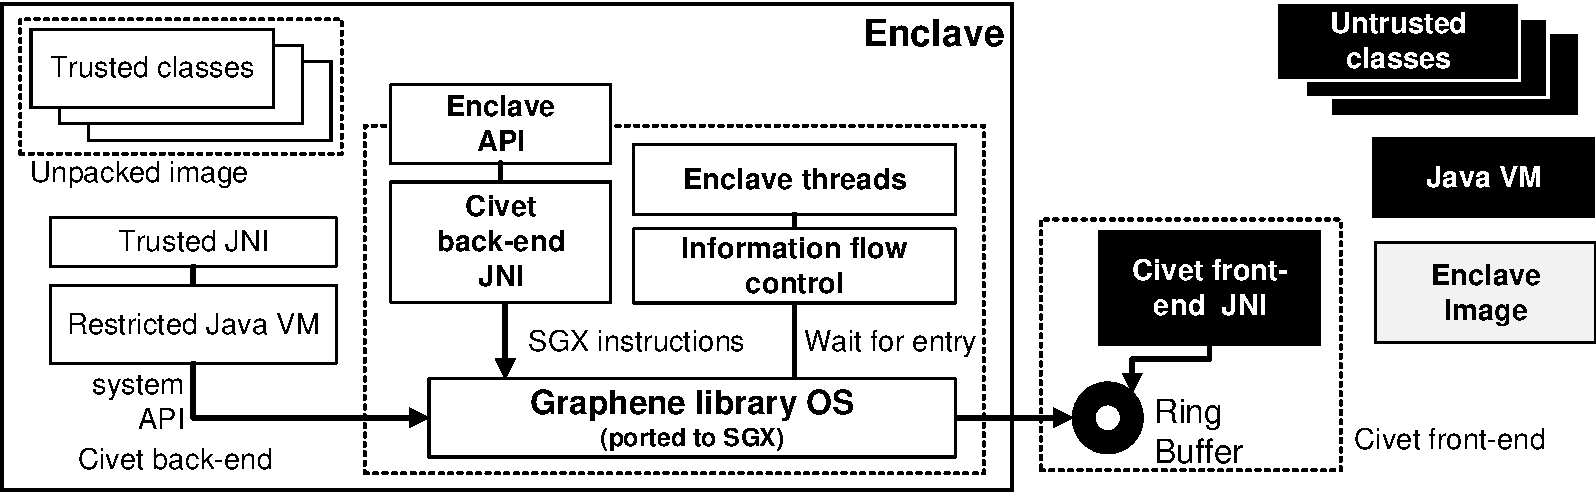
\includegraphics[width=4.5in]{civet/figures/civet-structure.pdf}
\caption[\sysname{}: framework overview.]
{\sysname{} framework overview.
\sysname{} creates two worlds for an partitioned \java{} application, each with an individual JVM.
The JVM in the enclave is ported using Graphene library OS.
Untrusted classes can invoke methods of trusted classes through proxy objects,
which can transparently access the enclave interface, through serialization
and deserialization over an ring buffer accessed by both untrusted JVM and trusted JVM. }
\label{fig:civet:runtime}
\end{figure}


\subsection{Seamless access to in-enclave objects}
\label{sec:civet:concept:interface}

For programmer convenience, 
untrusted code can seamlessly call in-enclave objects in \sysname{}.
This is particularly useful when application components are closed-source.
All public methods of trusted, programmer-identified entry classes are entry points for the enclave.
The \sysname{} runtime framework is responsible for generating glue code for entering and exiting
the enclave appropriately, tracking references to objects in the enclave, 
as well as marshalling arguments and return values for in-enclave functions.

%in \sysname{},
%access to in-enclave objects seamless for the untrusted components.
%The rationale behind this design is based on two reasons.
%First, the target of method invocation in \java{} is identified dynamically
%via referencing the object.
%Second, \sysname{} intends to avoid the developers' effort for injecting explicit entry points into the untrusted components,
%especially when the imported \java{} class libraries are close-source.

%% As \sysname{} dynamically determines the enclave entry points in the untrusted components,
%% it avoids the requirement for developers
%% to define the untrusted interface of the enclave.
%% Instead of inquiring manual definition,
%% \sysname{} applies a simple principle to automatically determine the entry points:
%% All public methods of the {\em public} trusted classes can be entry points of the enclave.

In order to reference objects inside the enclave from outside the enclave,
\sysname{} framework uses a byte code generation library --- {\em CGLib}~\citep{cglib} to create untrusted proxies for the in-enclave instances.
CGLib instruments the class that is being proxied,
and redirects the control to a handler 
assigned by \sysname{} upon any method invocation on the proxy.
The proxy then triggers enclave entry to run the trusted method.



%% When untrusted code calls a public method of a trusted class,
%% \sysname{} transparently identifies 
%% determines enclave entry based on whether the objects accessed is in the enclave or part of the untrusted components.
%% As classes can be replicated inside and outside the enclave,
%% the same method of the same class must trigger different behavior according to the sensitivity of the instances.
%% If the object is instantiated in the untrusted components, the method must be run outside the enclave.
%% If the object is instantiated in the enclave, the method should be trapped,
%% and trigger enclave entry to run the method.
 
In general, supporting classes can be duplicated inside and outside of the enclave.
Calls to a supporting class, such as {\tt String}, from inside of an enclave
go to the in-enclave version, and calls from outside the enclave go to the untrusted version.

An exception is made for entry classes, which are not allowed to be replicated.
Rather, any call to an entry class function is placed inside the enclave.
Thus, constructors and static methods of entry classes also cause enclave entries.
We note that this design point was taken to minimize programmer effort in porting to SGX;
alternatively, we could allow an entry class to be replicated by requiring the programmer to 
explicitly annotate calls to object functions.

The \sysname{} design-time tool creates untrusted proxy classes for all entry classes,
in which all constructors and static methods are redirected to
the \sysname{} front-end, which then enters the enclave.
We chose this approach because CGLib disallows redirecting 
constructors and static methods, as this can introduce ambiguity in
the invocation target when all classes are in the same JVM.

%% If the method called is a constructor or static method,
%% the affected object is no longer an instance,
%% but the class itself.
%% To allow seamless invocation of the method,
%% it causes ambiguity for the affiliation of the class, if the class is replicated in both partitions.
%% Therefore, \sysname{} restricts the invocation of constructors or static methods
%% to only the entry classes,
%% and disallows replicating the entry classes
%% in the untrusted components.
%% In addition, if the constructor of an entry class is called upon the constructor of its untrusted subclass,
%% the instantiation will be rejected by \sysname{}.

%% \paragraph{Interception of in-enclave objects.}
%% To seamlessly trigger the enclave entry upon method invocation,
%% \sysname{} intercepts the instances or classes that belong to the isolated components.
%% To intercept non-static method of in-enclave instances,
%% \sysname{} uses {\em CGLib} \fixme{cite} to create proxies of the in-enclave instances.
%% CGLib instruments the class that is being proxied,
%% and redirect the control to a handler assigned by \sysname{} upon any method invocation on the proxy.
%% The handler then triggers enclave entry to run the isolated method.

%% \sysname{} uses a different mechanism of interception for constructors and static methods,
%% because CGLib disallows redirecting constructors and static method
%% due to the ambiguity of invocation targets.
%% Instead, \sysname{} uses the design-time tool to create a dummy classes for all the entry classes,
%% in which all constructors and static methods are redirected to
%% the \sysname{} front-end.
%% Because we disallow replication of entry classes
%% in the untrusted components,
%% loading the dummy classes does not affect functionalities of the application. 

\paragraph{Passing arguments into the enclave.}
When a method triggers enclave entry, the arguments of the method have to be passed into the enclave for the invocation.
\sysname{} always copy the arguments into the enclave,
by serializing the arguments into byte streams,
copying the byte streams into the enclave memory,
and then de-serializing into objects.
By coping arguments into the enclave,
\sysname{} ensures execution of trusted code does not inadvertently leave the enclave.
If the code invokes a method on one of the arguments,
the in-enclave copy of the class is used on an in-enclave instantiation of the object.
Upon de-serialization, the arguments are also automatically type-checked,
thus avoiding the risk of memory corruption.

\paragraph{Returning objects.}
Once the triggered method finishes execution in the enclave,
it may return an object or literal back to the untrusted calling function.
In general, objects are returned similarly to passing input arguments---by serializing the object to a byte stream and returning the bytes.
%Technically, returning objects is the same as passing arguments, and only take serialization and de-serialization.

In order to ensure confidentiality of sensitive data, \sysname{} takes additional care to check
whether a returned object creates an unexpected control flow.
At enclave exit, \sysname{} only allows an object to be returned if it is not tainted with any secret data,
in which case the object is serialized and passed back to the caller.
Section~\ref{sec:civet:security} details our information flow tracking mechanism.

In cases where the object is tainted and an instance of a trusted class,
\sysname{} instead creates a reference in the enclave (to prevent garbage collection of the object internally),
and returns an opaque reference type, that causes the untrusted \sysname{} runtime to create a proxy out of the enclave.
This policy applies to all constructors.
If a proxy object is garbage collected, the destructor calls into the enclave to release the reference on the 
corresponding object in the enclave.
The \sysname{} untrusted runtime is responsible for translating any proxy objects passed as arguments to the enclave into opaque pointers,
which the in-enclave runtime then translates to local object references.

In the case of a tainted literal, we encrypt the plaintext return value concatenated with a nonce, using a temporary key, and return the ciphertext.
This encrypted literal can then be passed to subsequent enclave calls, where the value is decrypted as part of deserialization.

%% However, unconditionally allowing returning objects may become a threat to the information confidentiality of the enclave,
%% because the object may contain part of the enclave secrets due to the information flow.
%% \sysname{} only allows returning objects
%% that are not tainted by the information flow from any secrets. More details about determining the taintedness of the objects are discussed in section~\ref{sec:civet:security}.

%% Based on the taintedness of the objects, \sysname{} has different policies and mechanisms of returning the objects to the caller,
%% to maintain both information confidentiality and progress of the application.
%% The policies are described as follows:

%% \begin{compactitem}
%% \item {\bf the object is not tainted}: serialize and pass the object to the caller.
%% \item {\bf the object is tainted, and is instance of an isolated class}: 
%% create a proxy and intercept future invocation.
%% The policy commonly applies to all constructors.
%% \item {\bf the object is tainted, and is a literal}:
%% automatically encrypt the literal with a default key.
%% \end{compactitem}


%\paragraph{Secure entry and exit of the enclave}
%The \sgx{} hardware ensures that the enclave only has fixed number of entry points (exactly one location where the execution starts, but multiple pre-defined locations that the execution can jump to). 
%The untrusted components must be forbidden to jump to random code in the enclave.
%Moreover, if the isolated component want to exit the enclave,
%it must explicit call the exit instruction ({\tt EEXIT}) to make sure
%the control flow won't be manipulated to leave the enclave.

%\sysname{} models this guarantees by exporting all the public methods of the isolated classes
%(including constructors, static and non-static methods) as the entry points or untrusted interfaces.
%When the untrusted component calls a constructor or static method of an isolated class,
%the execution inside the enclave is triggered,
%either to instantiate the class or perform other operations.
%If a proxy of an isolated instance is returned to the untrusted components,
%the untrusted components can keep it or pass it around.
%As soon as any untrusted components call one of the public methods on the proxy, the execution re-enter the enclave and start the isolated execution.

%Exporting public methods as the entry points or the untrusted interface
%is assumed to be reasonably secure in \sysname{}.
%First, only for the entry classes (the top-most classes of the enclave),
%the constructors or static method will be exported.
%Because developers have expressed that these classes are the ones that interact with the untrusted classes, it is safe to allow the untrusted components to calls these methods and trigger execution in the enclave.
%Second, even if the public non-static methods can be called
%upon isolated classes, the untrusted components can only call upon the proxies,
%which are essentially returned values from the previous method calls.
%Without the proxy, the untrusted components can never call the public methods
%on random instances in the enclave, if the instances are never returned to the untrusted components.


\subsection{Remote Attestation and Provisioning}
\label{sec:civet:concept:others}

\paragraph{Generating attestation reports.}
A feature of \sgx{} hardware is the ability to generate an attestation report for a remote entity,
demonstrating the integrity of the enclave code at launch time.
%The \sgx{} hardware provides the feature of generating a attestation report to prove the integrity of the isolated execution to a remote entity.
\sysname{} provides helper API for developers to access these features,
with convenience and extended trust.
For attestation, \sysname{} generates a report that contains a list of classes loaded inside the enclave, with their measurements.
The report is attached with the attestation generated and signed by \sgx{}, but processed by Graphene.
The \sgx{}-generated attestation contains both
the enclave measurement (proving integrity of Graphene) and
the measurement verified by Graphene (proving integrity of other binaries and files).


%% \fixmedp{Huh?  Really?}
%% The attestation report contains the enclave measurement
%% and is signed using a key derived
%% from the measurements of both sides of attesters,
%% so the remote entity can verify it by retrieving the same key
%% (both attesters must be running in \sgx{} enclaves).

Note that \sysname{} also includes
the dynamic loading state in the attestation report.
%A stronger guarantee provided by \sysname{} than \sgx{}
%is to present the dynamic loading state in the attestation report.
The attestation generated by \sgx{} only contains
the initial state of the enclave, and does not record changes within the executable code
after the enclave starts. 
In both cases, the remote entity is trusting the initially loaded binary
to not dynamically load code that could compromise the enclave;
however, \sysname{} can offer a more precise accounting of the state of the enclave 
at the time a report is generated.

\fixmedp{For future work, would be cool to have some non-editable record of what is added to the enclave, so a corrupted enclave cannot hide the equivalent of a rootkit}

%% As a result, the entity that
%% verifies the attestation report has to blindly trust the initial code
%% in the enclave does not dynamically load any vulnerable code.  
%% The attestation report generated by \sysname{}
%% reflects the latest state of class loading,
%% allowing the trusted entity to audit the execution of enclaves.

% providing a class called {\tt Enclave}, with the APIs that service attestation and provisioning requests.
%The {\tt Enclave} APIs are wrapper to the low-level semantics required by the \sgx{} hardware,such as exchanging the attestations with remote hosts and verifying them, or 
%securing the channels after attesting the other side of communication.
%Because the works are completely hidden beneath the APIs,
%the developers are spared from all the cryptographic details during the process of attestation and provisioning.

\paragraph{Secure provisioning.}
\sysname{} provides an API that transparently validates a connection to a remote host to load
sensitive classes or secret data.
%to be used for secure provisioning.
To use this API, both sides of the connection
must be running in enclaves created by \sysname{}.
The API performs key exchange algorithm (e.g., Diffie-Hellman) on the connection,
secure the connection with encryption,
and authenticate the connection by exchanging the attestation reports.
\sysname{} provides convenient helper functions for developers to create a trusted path
for provisioning sensitive data to a remote enclave.
%Developers can use this API to design any provisioning scheme, without implementing the details of building the trusted path.


\section{Hardening \sgx{} at Enclave Boundary using Information Flow Control in \java{} }
\label{sec:civet:security}

\sysname{} % models the high-level security guarantees and features
%of the \sgx{} hardware in the \java{} language,
allows \java{} developers to directly utilize the security features of \sgx{}, such as isolation from an untrusted hypervisor, % execution, code integrity, etc,
in combination with language-level features that make the code in the enclave more robust.
% safety and advanced protections in \java{}.
%By bridging the gap between language and hardware protections,
%\sysname{} creates opportunities to combine \sgx{} hardware protections
%and security benefits given by \java{} as a managed language.
%In this section, we discussed the opportunities we explore to harden \sgx{} protection with the usage of \java{} language.

%\fixmedp{Honestly, a lot of this is getting pretty repetitive.  I would probably hoist the argument for Java into the motivational text and not bother repeating it here.}

%\subsection{Benefits from the usage of \java{} Language}

%We note that \java{} has several features that can reduce or eliminate
%common vulnerabilities.
%Memory corruption bugs are constant threats to applications
%implemented in C or C++ languages,
%but \java{} applications naturally defend against these vulnerabilities.
%\java{} is immune from memory corruption bugs, such as heap and buffer overflows.
%Several security enhancements come naturally with running \java{} classes
%in the enclave. \java{} applications are known to be immune to memory corruption bugs such as buffer or heap overflow.
%Type casting in \java{} is checked against the type of the target object.
%applications, \java{} perform strict type-checking on the objects to be casted.
%Type-checking prevents corruption of object either in the isolated components,
%or when receiving arguments from the untrusted interfaces.
%Similarly, 
%Similar as the memory corruption bugs,
%Because \java{} is memory safe, it is immune to known control flow attacks, such as return-oriented programming,
%where control flow is manipulated by unsafe writes to return pointers on the stack or function pointers in objects.
%applications implemented in C or C++ languages inevitably face the risk of ROP (return-oriented programming) attacks,
%where attackers can manipulate the control flow by corrupting the applications' stacks or heaps.
%Since \java{} classes can defend against memory corruption,
%attacks cannot manipulate the control flow by overriding the return pointers or function pointers.

%We do assume that the JVM and JNI code are free from memory corruption and control flow attacks.
%Proving a JVM implementation correct is beyond the scope, although similar 
%efforts have been made previously to prove a language runtime correct~\citep{yang10safe}.
%In the case of JNI, we would discourage developers from using JNI code in enclaves if at all possible.

%% Note that although memory corruption bugs and control flows attacks are forbidden in \java{} classes,
%% these vulnerabilities can still exist in the \java{} VM and JNI.
%% In \sysname{} we assume \java{} VM and JNI must be fully trusted,
%% and we leave it as a future work to secure these components.

%% dp: Meh.  prolix
%% For isolated components in the enclaves, memory corruption bugs and control flow attacks are just as dangerous as for other applications.
%% Because the isolated components are fully trusted by the CPU,
%% they can access any memory that are set to proper permissions, including the memory outside the enclaves.
%% Even if a vulnerable component is exploited to copy all the enclave secret out of the enclaves, no hardware solution can effectively stop the exploitation.
%% Even though isolated components cannot directly jump out of the enclave,
%% control flow attack can still manipulate the components to jump to certain locations internally and perform malicious operations. 
%% Therefore, preventing memory corruption bugs and control flow attacks
%% can be a strong reason for application developers
%% to choose \java{} language instead of C/C++ to implement the isolated components.

%\fixmedp{This whole subsection is already covered above.  Commenting}
\begin{comment}
\subsection{Reducing the enclave TCB}

%A \java{} applications often yield a huge TCB, including the \java{} VM,
%JNI and supporting classes that come in bulk.
%For example, a \java{} applications executed by \jvm{}
%will load the \java{} VM binaries up to 40MB \fixme{find out actual numbers}. The classes in the standard \java{} VM libraries such as {\tt rt.jar} includes more than 18,000 classes, and the size of the package is more than 30MB.
%On the other hand, the actual classes needed by an application from {\tt rt.jar}
%can be as less as 1,000 classes.
%Majority of the classes provided from {\tt rt.jar},
%--- even though they may never be loaded into the enclave ---
%still remains in the TCB.

Having unnecessary binaries and classes in the TCB of the enclave
can aggravate the risk of being attacks.
First of all, the huge amount of code loaded into the enclave
increase the opportunity of having gadgets that can be exploited in ROP attacks,  
which can still happen in the \java{} VM or JNI.
Even though most of the \java{} classes have static footprint of their supporting classes,
many of them still dynamically load classes, such as directly calling the class loader, or specifying providers to the \java{} cryptography framework.
Having huge TCB as \java{} classes in the enclave still intensify
the risk of attacks, even though \java{} classes are immune to control flow attacks. 

\sysname{} largely reduce the supporting classes that can be loaded into the enclave,
by partitioning out the necessary classes from all the libraries in the developers' class paths, into the enclave image.
When the enclave is created, the \java{} VM will not load any existing libraries such as {\tt rt.jar} from the host system,
but instead only search classes in the signed enclave image.
Minimizing the supporting classes that can be loaded into the enclave
guarantees that all the classes that are included in the TCB
are actually required by the isolated components,
and come from a trusted source such as the developers' execution environment. 

Note that we do not partition the JNI within the \java{} VM binaries.
We assume partitioning out the JNI functions that are required by the isolated classes
is fully feasible with some manageable efforts.
Moreover, the \java{} classes can be potentially partitioned at a smaller granularity than the whole classes, such as the methods and fields, which can even further reduce the TCB.
We leave these potential improvements as future works. 
\end{comment}

%\subsection{Information Flow Control at Enclave Boundary}
%Problem of not just leaking secrets but also tainted info
As an example of higher-level, language-based analysis, we implemented information flow tracking
in \sysname{}.
A common usage of enclaves is to protect sensitive data, such as an encryption key;
thus, a common concern is that this sensitive data not be inadvertently returned because of an error or exploit within the enclave code.
In general, we chose a design point that minimizes programmer effort; to adopt information flow tracking, we
do require the programmer to specify secret data classes and declassify objects to be released as is from the enclave.

\begin{figure}[t!]
\centering
\includegraphics[width=3.2in]{civet/figures/declassify.pdf}
\footnotesize
\caption[\sysname{}: declassifier APIs.]
{How \sysname{} provides declassifier APIs to declassify sensitive data.
When the untrusted class ({\tt Untrusted}) from Figure ~\ref{fig:civet:synthesis} now calls the {\tt encrypt} method of a trusted class ({\tt Trusted}),
\sysname{} automatically calls the {\tt encrypt} method inside enclave, and pass the {\tt String} parameter.
Before returning the result, the trusted class has to use the {\tt declassify} to remove the taint of {\tt tainted} variable that is tainted by the {\tt encrypt} method of class {\tt Encryptor} because of the tainted secret variable {\tt s}.
}
\label{fig:civet:declassify}
\end{figure}

%Because the code running in enclave has access to complete address space, including the trusted as well as untrusted memory regions, it is easy for the trusted code to inadvertently undermine \sgx{} protection by writing secret information in the untrusted region. Further, leaking any information derived from or related to the secret may be used by the untrusted code to guess the value of secret information. For example, even in the presence of memory protection, sandboxing and virtualization, it is possible to recover the secret key used by crypto algorithms~\citep{kocher1996timing,osvik2006cache,weiss2012cache, zhang2012cross}. So, to ascertain the secrecy of the sensitive data, no information derived from the secret should exit enclave in plaintext.

%We use JAVA tool phosphor source and sink to taint provisioned data and control leakage
%\sysname{} leverages extensive research on information flow tracking and control in \java{} to harden the \sgx{} security. 

In the enclave, we implement source-to-sink taint tracking, using the open-source Phosphor library~\citep{phosphor}.
%\fixmedp{check this}
The programmer manually selects the classes containing secret data that take secret input from a remotely-provisioned source.
This taint is propagated to any new variables that result from explicit or implicit flows from a secret object.
The only way to remove taint from an object is to pass the object through a \sysname{} declassifier API,
which returns an untainted copy of the object.

%\fixmedp{Would be nice to have a simple example class with a label and declassifier in a figure, if space and time allow}

\sysname{} enforces the policy that only untained data may be returned from an enclave.
If tainted data is being returned, the system transparently encrypts the data and removes its taint before letting the data leave the enclave.
In the cases where a developer wants to return references to sensitive data, \sysname{} instead returns an opaque reference or, in the case of a literal, encrypts the return value.

%mFor tainted data, the developer may opt to either throw a runtime error, or, by default, to return an encrypted object instead.
%The en

% to taint the secret data when provisioned and propagate the taint to any new data generated as an explicit or implicit result of the secret data. We specify the enclave exit points as targets and enforce the policy that any tainted data must pass through a declassifier, that encrypts the data before egress. We only consider the provisioned data as security sensitive, as the enclave image is only integrity protected.

%Declassifier API: correct usage and scenarios
The \sysname{} {\tt Enclave} class provides a {\tt declassify(Object o)} API that creates an untainted
copy of the object.  In practice, we expect this function to be used in conjunction with tests
on the returned data, or cryptographic functions to protect the data in transit across an untrusted channel.

Continuing our example from Figure~\ref{fig:civet:synthesis}, in Figure~\ref{fig:civet:declassify}, if the {\tt Untrusted} class wants to call the {\tt encrypt} method on the trusted object {\tt t}, \sysname{} front-end transparently passes the argument string {\tt o} to the enclave, and the corresponding {\tt encrypt} method is called in the enclave. The secret {\tt s} is tainted because it was provisioned from remote trusted server as shown in Figure ~\ref{fig:civet:synthesis}. As a result, the call to method {\tt encrypt} of class {\tt Encryptor} taints the encrypted output string {\tt tainted}. If the developer had returned this {\tt tainted} variable, the \sysname{} information flow tracking would re-encrypt the ciphertext, and thus make the return value useless for the {\tt Untrusted} class. However, as the developer wants to return the ciphertext as is, she can declassify the {\tt tainted} string by passing it through the declassifier API to get an untainted version of the same object. Such untainted objects can be released from the enclave without further encryption.

%to let the application developer explicitly indicate that the argument object does not contain any secret information, and is safe to leave the enclave as is. For instance, if the enclave code encrypts a blob of data using the tainted secret provisioned key, the information flow will taint the encrypted data. However, because the encrypted data is safe to exit enclave if a perfectly secure encryption algorithm is used, the developer can explicitly mark the encrypted data as declassified. We note that the developers need to be extra careful while declassifying objects to inadvertently leaking secret information.

%Dealing with confidential code
In order to protect the confidentiality of sensitive code,
\sysname{} also allows classes themselves to be tainted.
\sysname{} enforces a policy that any data returned from sensitive code is tainted, and the developer needs to explicitly declassify tainted output data to mitigate
concerns around reverse-engineering the code based on brute-force probing of its outputs.
Of course, the binary code itself is also not allowed to be copied out of the enclave.

% expose it to the untrusted world.
%The {\em code confidentiality} property of \sysname{} loads and executes encrypted classes from remote hosts to protect secret algorithm. We consider this provisioned code as equally security sensitive as provisioned data. ~

%\begin{table*}[t!b!]
\centering
  \begin{tabular}{p{0.05in} >{\raggedright\arraybackslash}p{2.05in} >{\raggedright\arraybackslash}p{4.4in}}
  \toprule
  \multicolumn{2}{l}{\it Security guarantees or features} & {\it The modeling approach applied by \sysname{}} \\
  \midrule
  \midrule
  \multicolumn{3}{l}{\bf Natively provided by the \sgx{} hardware (including the SDK):} \\
  \midrule
  & Isolating security-sensitive components &
  Asking developers to identify multi-level sensitivity, by marking the {\em entry classes}. Complete separation between isolated and untrusted classes.
  \\
  \midrule
  & Secure entry / exit of enclaves &
  Exporting public methods of isolated classes. Arguments are type-checked.
  \\
  \midrule
  & Integrity of the execution environment & 
  Packaging all supporting classes into a signed JAR.
  \\
  \midrule
  & Attestation \& secure provisioning & 
  Providing class {\tt Enclave}, to create secure channels and exchange attestation.
  \\
  \midrule
  \midrule
  \multicolumn{3}{l}{\bf Improvement from combining of \java{} language and the \sgx{} hardware protection:} \\
  \midrule
  & Memory safety \& control flow integrity &
  Naturally provided by \java{} language.
  \\
  \midrule
  & Reducing the enclave TCB &
  Automated partitioning based on class dependencies.
  \\
  \midrule
  & Preventing information flow leakage &
  Tracking information flow in trusted classes, only allow releasing the information if not tainted or declassified by developers.
  \\
  \midrule
  & Code confidentiality & Dynamically loading provisioned classes.
  \\
  \end{tabular}
  
\footnotesize
\caption{
The approaches applied by \sysname{} to model the security guarantees and features of the \sgx{} hardware, and to enhance the security by combining language and hardware protections.
}
\label{tab:features}
\end{table*}


%% dp: This title is pretty vague.  
%\section{Addressing the Combination of \java{} and \sgx{}}
\section{\java{} Support for Partitioning into \sgx{}}
\label{sec:concept}

%\fixmets{1.5 page}

This section explains the support \sysname{} adds to \java{}
for partitioning applications into \sgx{} enclaves.
%support in addresses the challenges
%in partitioning \java{} applications on 

\subsection{Cleanly partitioning classes and objects}
\label{sec:concept:partition}

%To address the partition challenge in a managed language like \java{},
%\sysname{} diminishes the need for developers
%to scrutinize the whole code base
%and identify the fine line of isolating trusted and untrusted classes. 

\sysname{} includes Shredder to 
 partition \java{} code for \sgx{},
reducing developer effort.
Figure~\ref{fig:builder} shows the workflow of a developer using the \sysname{} Shredder tool.
The developer selects the application's main class, either as a JAR or class files
and the classpath of the library.
The developer also specifies the list of
entry classes that should be in the enclave and exports an interface to the code 
outside of the enclave.
%% When developers use the tool to partition their applications, they provide
%% the application package, either in JAR or classes,
%% the class paths of the depended libraries,
%% and a list of {\em entry classes} as the initial entry points of the enclave.
The Shredder then
identifies all classes that the entry classes depend upon,
until the transitive closure of these dependencies converges.
%performs {\bf dependency tracking} starting at the entry classes,
%until all the depended classes eventually converge.
%% dp: this feels out of place here; maybe put it at the beginning of the section?
%Afterward, \sysname{} packages the classes, with additional steps of augmentation, instrumentation, and signing, purpose of which is explain in \S\ref{sec:concept:loading} and \ref{sec:concept:accessing}.

\begin{figure}[t!]
\centering
\includegraphics[width=1.0\linewidth]{building-tool.pdf}
\caption{\sysname{} \staticphase{} tool, for partitioning, packaging, augmentation, instrumentation, and signing.
\sysname{} partitions the \java{} application based on the entry classes
specified by the developers (classes {\tt Trusted}).
The Shredder tool recursively pulls all required supporting classes into the 
package to run in the enclave.
%from all the class paths.
%Only the minimum necessary classes are kept for the enclave,
The Shredder tool creates an enclave JAR file after augmentation,
instrumentation, and signing.}
\label{fig:builder}
\end{figure}

The Shredder creates a single package with all dependencies of the
entry classes.
This is a reasonable simplification, although 
% for two reasons.  First, 
%loading all required classes from a single package is 
%is a reasonable simplification 
%that matches expected practice for enclaves.
%We note that 
it would be relatively easy in future work to add multiple, signed JAR-style packages,
if needed.
This approach also allows us to 
reduce the attack surface and overheads by minimizing the 
enclave entry and exit points, albeit at the expense of duplicating some supporting
classes in and out of the enclave.
%\fixmedp{sounds like we don't let enclave code call out to classes? Might bear some discussion whether this is a limitation or not}

%% We argue that partition based on entry classes and
%% dependency tracking at class granularity
%% is sufficient for isolating the trusted and untrusted components.
%% There are basically two goals for our partition tool:

%% \begin{compactenum}
%% \item To create a static package of supporting classes, so the \sysname{} \dynamicphase{} framework can load every required class from the package.
%% \item To avoid the isolated execution from leaving the enclave,
%% in between the entry triggered by method invocation
%% from the untrusted components,
%% and returning the control to the untrusted components.
%% \end{compactenum}


Unless the application explicitly asks the class loader to
dynamically load a class,
every piece of code needed during the execution of trusted classes
is included in the enclave image.
The image includes classes that are used in dynamic casting and parent classes 
that contain code inherited by the trusted classes.
Shredder also includes any required supporting JNI libraries in the image.
Shredder does not attempt to partition the JNI libraries to a smaller binary,
which we leave for future work.

%Because \java{} maintains type-safety in most cases \fixmedp{is it not always type safe?},
%any classes that have ever been cast to in the application can be tracked as a dependency. Methods that are inherited from the parent classes
%are also covered in dependency tracking.

%If an application will ever request for dynamic loading using class names,
%the developers must specify the classes in the partition tool.
%The case that dynamic loading is needed is most commonly seen in the crypto APIs:
%for example, to instantiate a {\tt Cipher} object,
%the applications will provide a string that describes the transformation
%of the cipher, such as {\tt AES/CBC/PKCS5PADDING}.
%Based on the string, the method {\tt Cipher.getInstance()} will load classes
%{\tt AESCipher}, {\tt PCBC}, and {\tt PKCS5Padding}.
%The rationale behind dynamic loading is that no matter
%which class name the application request for,
%the class loader will only search among the trusted classes,
%so no malicious classes will be loaded.

%% \sysname{} also includes any JNI 
%% In the case that any supporting classes require JNI,
%% \sysname{} will include the correspondent JNI libraries in the enclave image.
%% The JNI libraries are unpacked when the enclave starts,
%% and added to {\tt LD\_LIBRARY\_PATH} for the trusted \jvm{}.
%% \sysname{} currently does not partition the JNI libraries, but we see the partition of JNI as a manageable future work. 

Based on our case studies (\S\ref{sec:case-study}),
we observe that specifying the entry classes and identifying any dynamically loaded classes,
is relatively simple.  %requires low developer effort.
In all of our use cases, the applications are partitioned with only one entry class, and very few dynamically loaded classes.


%\sysname{} transparently handles all the details of accessing \sgx{} hardware,
%in behave of the loaded \java{} applications (as shown in figure~\ref{fig:synthesis}).
%When \sysname{} is called to run isolated \java{} components,
%it creates two worlds of \java{} execution --- one is in the enclave and the other is outside the enclave.
%With the ability of running \java{} classes inside the enclave,
%\sysname{} can support the partitioned model with both isolated and untrusted classes implemented as \java{} classes.

%\begin{table*}[t!b!]
\centering
  \begin{tabular}{p{0.05in} >{\raggedright\arraybackslash}p{2.05in} >{\raggedright\arraybackslash}p{4.4in}}
  \toprule
  \multicolumn{2}{l}{\it Security guarantees or features} & {\it The modeling approach applied by \sysname{}} \\
  \midrule
  \midrule
  \multicolumn{3}{l}{\bf Natively provided by the \sgx{} hardware (including the SDK):} \\
  \midrule
  & Isolating security-sensitive components &
  Asking developers to identify multi-level sensitivity, by marking the {\em entry classes}. Complete separation between isolated and untrusted classes.
  \\
  \midrule
  & Secure entry / exit of enclaves &
  Exporting public methods of isolated classes. Arguments are type-checked.
  \\
  \midrule
  & Integrity of the execution environment & 
  Packaging all supporting classes into a signed JAR.
  \\
  \midrule
  & Attestation \& secure provisioning & 
  Providing class {\tt Enclave}, to create secure channels and exchange attestation.
  \\
  \midrule
  \midrule
  \multicolumn{3}{l}{\bf Improvement from combining of \java{} language and the \sgx{} hardware protection:} \\
  \midrule
  & Memory safety \& control flow integrity &
  Naturally provided by \java{} language.
  \\
  \midrule
  & Reducing the enclave TCB &
  Automated partitioning based on class dependencies.
  \\
  \midrule
  & Preventing information flow leakage &
  Tracking information flow in trusted classes, only allow releasing the information if not tainted or declassified by developers.
  \\
  \midrule
  & Code confidentiality & Dynamically loading provisioned classes.
  \\
  \end{tabular}
  
\footnotesize
\caption{
The approaches applied by \sysname{} to model the security guarantees and features of the \sgx{} hardware, and to enhance the security by combining language and hardware protections.
}
\label{tab:features}
\end{table*}


%Even though \sysname{} hides the low-level semantics of the \sgx{} hardware from the applications,
%the applications still have full access to the security guarantees ({\em what is secured?}) and features ({\em how is it secured?}) provided by the the \sgx{} hardware.
%We do so by identifying the high-level goals of these guarantees and features,
%and remodel the goals in the \java{} language.
%The underlying mechanisms of these goals is the original guarantees and features provided by the \sgx{} hardware.

%We discuss each security guarantee or features of the \sgx{} hardware,
%and how they are actually modeled in \sysname{} as follows.

%\paragraph{Isolated execution of security-sensitive components}
%The \sgx{} hardware ensures components with higher security sensitivity
%to be executed inside the enclave
%and completely isolated from the components that are less security sensitive.
%The isolated components shall not share any data with the untrusted components unless the isolated components decide
%to flow the data out of the enclave.  

%\sysname{} models this guarantee by asking the developers to make
%the classes that they believe to be security sensitive.
%Note that only the top-most classes that interact with the untrusted components have to be identified --- we can these classes as the {\em entry classes}.
%After developers identifying the multi-level security sensitive with an application, \sysname{} uses a building tool to partition the application
%based on the developers' hint.
%The partition completely separates the \java{} classes for the isolated components from the classes for the untrusted components.
%The execution of these isolated classes will be fully jailed inside the enclave, and any invocation of the methods exported by the isolated classes
%from the untrusted classes
%will be re-routed into the enclave.
%The returned values of the invoked methods will be routed back to
%the untrusted classes,
%either as proxies of the actually returned instances (if the instances are not yet safe to release from the enclave) or the actual values.



\subsection{Dynamically loading byte-code with integrity}
\label{sec:concept:loading}

A key motivation for dynamic loading is the ability to load encrypted
classes from a remote, trusted host. 
For instance, one may want to load proprietary code into an enclave
that must first be decrypted and then validated, in order to 
protect an implementation of a trade secret.

Shredder creates a partition image as a JAR file, which
developers can ship with the rest of the application.
The application is then executed on an untrusted host with the 
%to the untrusted hosts that have the 
\sysname{} \dynamicphase{} framework installed.
%Then, on the untrusted hosts users will run the application,
Upon the first use, either by creating a trusted object or calling a static method of a trusted class,
%Whenever an entry class is instantiated, or one of its static method is invoked,
the \sysname{} \dynamicphase{} framework creates an enclave containing the trusted classes.

%\fixmedp{Trusted and isolated are used pretty interchangeably.  Pick one keyword and use it consistently, please}

Figure~\ref{fig:runtime} shows the structure of the \sysname{} \dynamicphase{} framework (a more detailed view of Figure~\ref{fig:synthesis}).
The \sysname{} runtime framework is split into the front-end (untrusted) and the back-end (trusted).
When the front-end calls into a trusted class,
it finds enclave image that contains the class,
checks if an enclave is created for the same image in the current \jvm{},
and, if not, creates an enclave.
The trusted classes from the same image share an enclave.
%and \sysname{} does not support the scenarios that the developers want to 
%further partition the trusted classes.

\sysname{} runs a separate, lighter-weight \jvm{} in the enclave.
Running a \jvm{} in the enclave is a subtle challenge because a \jvm{}
often yields a large system API footprint, and, by default, uses a large heap. % requires access to abundant resources such as the heap.
To provide the required OS APIs inside the enclave, we use the \graphene{} \libos{}~\cite{tsai14graphene}~\footnote{Downloaded from \url{github.com/oscarlab/graphene}}.
In order to remove unneeded features and balance resource utilization with performance in current \sgx{} enclaves, such as
a 128 MB limit on the size of the enclave page cache,
we adjust the build-time configuration of the \jvm{} to change multi-threaded garbage collector to single threaded, remove multiple JIT engines and stop non-essential threads in the \jvm{}. 
\fixmedp{say how, more specifically (in English.  You don't need to list specific options, but give us a bit more here}

%Moreover, a production \jvm{} like \jvmname{} is implemented in
%millions of lines of code \fixmets{get the actual number},
%which will cost tremendous effort to port into \sgx{} enclaves.

%To avoid the cost of porting the \jvm{}, \sysname{} uses {\em \sgx{}-\sgx{} \sgx{}}~\cite{graphene-sgx} 
%to facilitate the OS features needed by the \jvm{}.
%Therefore, we do not modify any code of \jvmname{}, except tuning the compilation options to reduce its resource usage.

%\fixmets{I am gonna avoid saying \sgx{} from now on.}
When \sysname{} creates an enclave, the \sgx{} hardware measures integrity of the initially-loaded \libos{}.
The \libos{} then loads \jvmname{} and all of the supporting libraries,
such as {\tt libc},
the JLI (\java{} legacy interface) library, and the minimal \java{} classes needed to bootstrap the class loader.
Finally, \jvm{} loads the enclave image JAR file.

The \graphene{} \libos{} maintains the code integrity of the \jvm{}.
When \graphene{} loads a binary or class files,
it verifies the integrity of the files by checking their measurements.
The measurements of binary or class files are also
hashed into the enclave measurement,
so no attacks can bypass the integrity check or manipulate \graphene{} to load  a malicious \jvm{} or bogus enclave image.

If an application requests dynamic loading by a class name,
the developers must specify the classes to the Shredder tool.
The case where dynamic loading is needed is most commonly seen in the crypto APIs:
for example, to instantiate a {\tt Cipher} object,
the applications provide a string that describes the transformation
of the cipher, such as {\tt AES/CBC/PKCS5PADDING}.
Based on the string, the method {\tt Cipher.getInstance()} loads classes
{\tt AESCipher}, {\tt PCBC}, and {\tt PKCS5Padding}.
The rationale behind this restriction on dynamic loading is that, no matter
which class name the application requests,
the class loader only searches among the trusted classes,
so no malicious classes will be loaded.
\fixmedp{Seems like you could also do a signature check at \dynamicphase{}, and there are other ways to relax this requirement, but whatever.}

%\paragraph{Integrity of the execution environment}
%The \sgx{} hardware must guarantee the execution of the isolated components
%is exactly the same as developed, tested and verified by the application developers.
%The \sgx{} hardware verify the cryptographic measurement of loaded binaries
%at the creation of the enclave,
%and can generate attestation that the enclave is created with such measurement.
%The purpose of the guarantee is to prevent code injection,
%unless the isolated applications are tricked into loading the code by the attackers.

%\sysname{} models this guarantee by creating a snapshot of developers'
%execution environment, including the version of \jvm{},
%checksums of any infrastructure binaries,
%and the minimal supporting classes for the isolated component. 
%\sysname{} packs all these files into a JAR file and sign it with the developers' private key.
%When \sysname{} creates an enclave, the hardware measurement of the enclave includes only the infrastructure, as the \jvm{} and the \sysname{} back-end.
%Once the enclave is created, the \sysname{} back-end must  
%check whether the JAR file loaded has the correct signature.

\begin{figure}[t!]
\centering
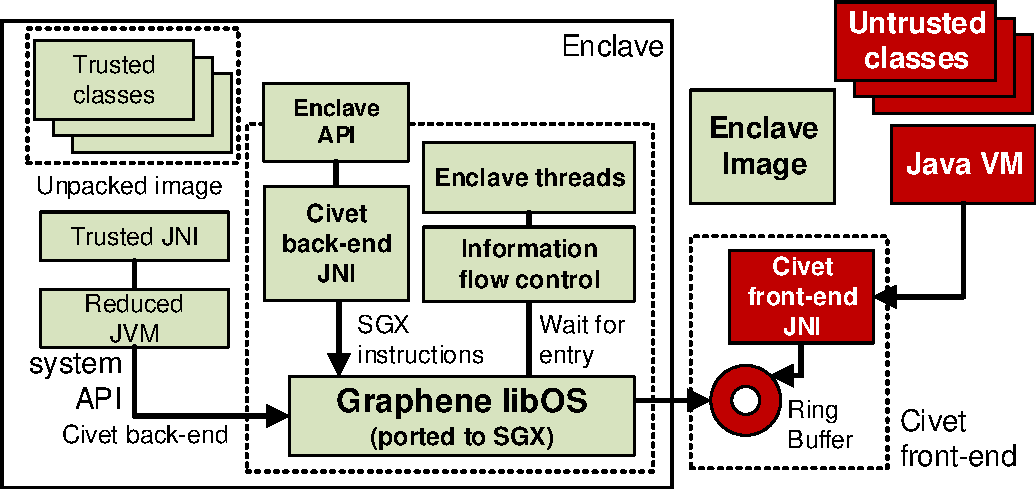
\includegraphics[width=1.0\linewidth]{civet-structure.pdf}
\caption{\sysname{} framework overview.
\sysname{} creates two worlds for a partitioned \java{} application, each with an individual \jvm{}.
The \jvm{} in the enclave is ported using the \graphene{} \libos{}.
Untrusted classes can invoke methods of trusted classes through proxy objects,
which can transparently access the enclave interface, through serialization
and deserialization over a ring buffer accessed by both untrusted and trusted \jvm{}. }
\label{fig:runtime}
\end{figure}


\subsection{Seamless access to in-enclave objects}
\label{sec:concept:accessing}

For programmer convenience, 
untrusted code can seamlessly call in-enclave objects in \sysname{}.
This is particularly useful when application components are closed-source.
All public methods of trusted, programmer-identified entry classes are entry points for the enclave.
The \sysname{} \dynamicphase{} framework is responsible for generating glue code for entering and exiting
the enclave appropriately, tracking references to objects in the enclave, 
as well as marshalling arguments and return values for in-enclave functions.

%in \sysname{},
%access to in-enclave objects seamless for the untrusted components.
%The rationale behind this design is based on two reasons.
%First, the target of method invocation in \java{} is identified dynamically
%via referencing the object.
%Second, \sysname{} intends to avoid the developers' effort for injecting explicit entry points into the untrusted components,
%especially when the imported \java{} class libraries are close-source.

%% As \sysname{} dynamically determines the enclave entry points in the untrusted components,
%% it avoids the requirement for developers
%% to define the untrusted interface of the enclave.
%% Instead of inquiring manual definition,
%% \sysname{} applies a simple principle to automatically determine the entry points:
%% All public methods of the {\em public} trusted classes can be entry points of the enclave.

In order to reference objects inside the enclave from outside the enclave,
\sysname{} framework uses a byte code generation library --- {\em CGLib}~\cite{cglib} to create untrusted proxies for the in-enclave instances.
CGLib instruments the class that is being proxied,
and redirects the control to a handler 
assigned by \sysname{} upon any method invocation on the proxy.
The proxy then triggers enclave entry to run the trusted method.



%% When untrusted code calls a public method of a trusted class,
%% \sysname{} transparently identifies 
%% determines enclave entry based on whether the objects accessed is in the enclave or part of the untrusted components.
%% As classes can be replicated inside and outside the enclave,
%% the same method of the same class must trigger different behavior according to the sensitivity of the instances.
%% If the object is instantiated in the untrusted components, the method must be run outside the enclave.
%% If the object is instantiated in the enclave, the method should be trapped,
%% and trigger enclave entry to run the method.
 
In general, supporting classes can be duplicated inside and outside of the enclave.
Calls to a supporting class, such as {\tt String}, from inside of an enclave
go to the in-enclave version, and calls from outside the enclave go to the untrusted version.

An exception is made for entry classes, which are not allowed to be replicated.
Rather, any call to an entry class function is placed inside the enclave.
Thus, constructors and static methods of entry classes also cause enclave entries.
We note that this design point was taken to minimize programmer effort in porting to \sgx{};
alternatively, we could allow an entry class to be replicated by requiring the programmer to 
explicitly annotate calls to object functions.

The Shredder creates untrusted proxy classes for all entry classes,
in which all constructors and static methods are redirected to
the \sysname{} front-end, which then enters the enclave.
We chose this approach because CGLib disallows redirecting 
constructors and static methods, as this can introduce ambiguity in
the invocation target when all classes are in the same \jvm{}.

%% If the method called is a constructor or static method,
%% the affected object is no longer an instance,
%% but the class itself.
%% To allow seamless invocation of the method,
%% it causes ambiguity for the affiliation of the class, if the class is replicated in both partitions.
%% Therefore, \sysname{} restricts the invocation of constructors or static methods
%% to only the entry classes,
%% and disallows replicating the entry classes
%% in the untrusted components.
%% In addition, if the constructor of an entry class is called upon the constructor of its untrusted subclass,
%% the instantiation will be rejected by \sysname{}.

%% \paragraph{Interception of in-enclave objects.}
%% To seamlessly trigger the enclave entry upon method invocation,
%% \sysname{} intercepts the instances or classes that belong to the isolated components.
%% To intercept non-static method of in-enclave instances,
%% \sysname{} uses {\em CGLib} \fixmets{cite} to create proxies of the in-enclave instances.
%% CGLib instruments the class that is being proxied,
%% and redirect the control to a handler assigned by \sysname{} upon any method invocation on the proxy.
%% The handler then triggers enclave entry to run the isolated method.

%% \sysname{} uses a different mechanism of interception for constructors and static methods,
%% because CGLib disallows redirecting constructors and static method
%% due to the ambiguity of invocation targets.
%% Instead, \sysname{} uses the \staticphase{} tool to create a dummy classes for all the entry classes,
%% in which all constructors and static methods are redirected to
%% the \sysname{} front-end.
%% Because we disallow replication of entry classes
%% in the untrusted components,
%% loading the dummy classes does not affect functionalities of the application. 

\paragraph{Passing arguments into the enclave}
When a method triggers enclave entry, the arguments of the method have to be passed into the enclave for the invocation.
\sysname{} always copy the arguments into the enclave,
by serializing the arguments into byte streams,
copying the byte streams into the enclave memory,
and then de-serializing into objects.
By coping arguments into the enclave,
\sysname{} ensures execution of trusted code does not inadvertently leave the enclave.
If the code invokes a method on one of the arguments,
the in-enclave copy of the class is used on an in-enclave instantiation of the object.
Upon de-serialization, the arguments are also automatically type-checked,
thus avoiding the risk of memory corruption.

\paragraph{Returning objects}
Once the triggered method finishes execution in the enclave,
it may return an object or literal back to the untrusted calling function.
In general, objects are returned similarly to passing input arguments---by serializing the object to a byte stream and returning the bytes.
%Technically, returning objects is the same as passing arguments, and only take serialization and de-serialization.

In order to ensure confidentiality of sensitive data, \sysname{} takes additional care to check
whether a returned object creates an unexpected control flow.
At enclave exit, \sysname{} only allows an object to be returned if it is not tainted with any secret data,
in which case the object is serialized and passed back to the caller.
Section~\ref{sec:security} details our information flow tracking mechanism.

In cases where the object is tainted and an instance of a trusted class,
\sysname{} instead creates a reference in the enclave (to prevent garbage collection of the object internally),
and returns an opaque reference type, that causes the untrusted \sysname{} runtime to create a proxy out of the enclave.
This policy applies to all constructors.
If a proxy object is garbage collected, the destructor calls into the enclave to release the reference on the 
corresponding object in the enclave.
The \sysname{} untrusted components are responsible for translating any proxy objects passed as arguments to the enclave into opaque pointers,
which the in-enclave components then translate to local object references.

%In the case of a tainted literal, we encrypt the plaintext return value concatenated with a nonce, using a temporary key, and return the ciphertext.
%This encrypted literal can then be passed to subsequent enclave calls, where the value is decrypted as part of deserialization.

%% However, unconditionally allowing returning objects may become a threat to the information confidentiality of the enclave,
%% because the object may contain part of the enclave secrets due to the information flow.
%% \sysname{} only allows returning objects
%% that are not tainted by the information flow from any secrets. More details about determining the taintedness of the objects are discussed in section~\ref{sec:security}.

%% Based on the taintedness of the objects, \sysname{} has different policies and mechanisms of returning the objects to the caller,
%% to maintain both information confidentiality and progress of the application.
%% The policies are described as follows:

%% \begin{compactitem}
%% \item {\bf the object is not tainted}: serialize and pass the object to the caller.
%% \item {\bf the object is tainted, and is instance of an isolated class}: 
%% create a proxy and intercept future invocation.
%% The policy commonly applies to all constructors.
%% \item {\bf the object is tainted, and is a literal}:
%% automatically encrypt the literal with a default key.
%% \end{compactitem}


%\paragraph{Secure entry and exit of the enclave}
%The \sgx{} hardware ensures that the enclave only has fixed number of entry points (exactly one location where the execution starts, but multiple pre-defined locations that the execution can jump to). 
%The untrusted components must be forbidden to jump to random code in the enclave.
%Moreover, if the isolated component want to exit the enclave,
%it must explicit call the exit instruction ({\tt EEXIT}) to make sure
%the control flow won't be manipulated to leave the enclave.

%\sysname{} models this guarantees by exporting all the public methods of the isolated classes
%(including constructors, static and non-static methods) as the entry points or untrusted interfaces.
%When the untrusted component calls a constructor or static method of an isolated class,
%the execution inside the enclave is triggered,
%either to instantiate the class or perform other operations.
%If a proxy of an isolated instance is returned to the untrusted components,
%the untrusted components can keep it or pass it around.
%As soon as any untrusted components call one of the public methods on the proxy, the execution re-enter the enclave and start the isolated execution.

%Exporting public methods as the entry points or the untrusted interface
%is assumed to be reasonably secure in \sysname{}.
%First, only for the entry classes (the top-most classes of the enclave),
%the constructors or static method will be exported.
%Because developers have expressed that these classes are the ones that interact with the untrusted classes, it is safe to allow the untrusted components to calls these methods and trigger execution in the enclave.
%Second, even if the public non-static methods can be called
%upon isolated classes, the untrusted components can only call upon the proxies,
%which are essentially returned values from the previous method calls.
%Without the proxy, the untrusted components can never call the public methods
%on random instances in the enclave, if the instances are never returned to the untrusted components.


\subsection{Remote Attestation and Provisioning}
\label{sec:concept:others}

\paragraph{Generating attestation reports}
A feature of \sgx{} hardware is the ability to generate an attestation report for a remote entity,
demonstrating the integrity of the enclave code at launch time.
%The \sgx{} hardware provides the feature of generating a attestation report to prove the integrity of the isolated execution to a remote entity.
\sysname{} provides helper API for developers to access these features,
with convenience and extended trust.
For attestation, \sysname{} generates a report that contains a list of classes loaded inside the enclave, with their measurements.
The report is attached with the attestation generated and signed by \sgx{}, but processed by \graphene{}.
The \sgx{}-generated attestation contains both
the enclave measurement (proving integrity of \sgx{}) and
the measurement verified by \sgx{} (proving integrity of other binaries and files).


%% \fixmedp{Huh?  Really?}
%% The attestation report contains the enclave measurement
%% and is signed using a key derived
%% from the measurements of both sides of attesters,
%% so the remote entity can verify it by retrieving the same key
%% (both attesters must be running in \sgx{} enclaves).

Note that \sysname{} also includes
the dynamic loading state in the attestation report.
%A stronger guarantee provided by \sysname{} than \sgx{}
%is to present the dynamic loading state in the attestation report.
The attestation generated by \sgx{} only contains
the initial state of the enclave, and does not record changes within the executable code
after the enclave starts. 
In both cases, the remote entity is trusting the initially loaded binary
to not dynamically load code that could compromise the enclave;
however, \sysname{} can offer a more precise accounting of the state of the enclave 
at the time a report is generated.

\fixmedp{For future work, would be cool to have some non-editable record of what is added to the enclave, so a corrupted enclave cannot hide the equivalent of a rootkit}

%% As a result, the entity that
%% verifies the attestation report has to blindly trust the initial code
%% in the enclave does not dynamically load any vulnerable code.  
%% The attestation report generated by \sysname{}
%% reflects the latest state of class loading,
%% allowing the trusted entity to audit the execution of enclaves.

% providing a class called {\tt Enclave}, with the APIs that service attestation and provisioning requests.
%The {\tt Enclave} APIs are wrapper to the low-level semantics required by the \sgx{} hardware,such as exchanging the attestations with remote hosts and verifying them, or 
%securing the channels after attesting the other side of communication.
%Because the works are completely hidden beneath the APIs,
%the developers are spared from all the cryptographic details during the process of attestation and provisioning.

\paragraph{Secure provisioning}
\sysname{} provides an API that transparently validates a connection to a remote host to load
sensitive classes or secret data.
%to be used for secure provisioning.
To use this API, both sides of the connection
must be running in enclaves created by \sysname{}.
The API performs key exchange algorithm (e.g., Diffie-Hellman) on the connection,
secure the connection with encryption,
and authenticate the connection by exchanging the attestation reports.
\sysname{} provides convenient helper functions for developers to create a trusted path
for provisioning sensitive data to a remote enclave.
%Developers can use this API to design any provisioning scheme, without implementing the details of building the trusted path.


\section{Filtering Information Flow at Enclave Border}
\label{sec:security}

\sysname{} % models the high-level security guarantees and features
%of the \sgx{} hardware in the \java{} language,
allows \java{} developers to directly utilize the security features of \sgx{}, such as isolation from an untrusted hypervisor, % execution, code integrity, etc,
in combination with language-level features that make the code in the enclave more robust.
% safety and advanced protections in \java{}.
%By bridging the gap between language and hardware protections,
%\sysname{} creates opportunities to combine \sgx{} hardware protections
%and security benefits given by \java{} as a managed language.
%In this section, we discussed the opportunities we explore to harden \sgx{} protection with the usage of \java{} language.

%\fixmedp{Honestly, a lot of this is getting pretty repetitive.  I would probably hoist the argument for Java into the motivational text and not bother repeating it here.}

%\subsection{Benefits from the usage of \java{} Language}

%We note that \java{} has several features that can reduce or eliminate
%common vulnerabilities.
%Memory corruption bugs are constant threats to applications
%implemented in C or C++ languages,
%but \java{} applications naturally defend against these vulnerabilities.
%\java{} is immune from memory corruption bugs, such as heap and buffer overflows.
%Several security enhancements come naturally with running \java{} classes
%in the enclave. \java{} applications are known to be immune to memory corruption bugs such as buffer or heap overflow.
%Type casting in \java{} is checked against the type of the target object.
%applications, \java{} perform strict type-checking on the objects to be casted.
%Type-checking prevents corruption of object either in the isolated components,
%or when receiving arguments from the untrusted interfaces.
%Similarly, 
%Similar as the memory corruption bugs,
%Because \java{} is memory safe, it is immune to known control flow attacks, such as return-oriented programming,
%where control flow is manipulated by unsafe writes to return pointers on the stack or function pointers in objects.
%applications implemented in C or C++ languages inevitably face the risk of ROP (return-oriented programming) attacks,
%where attackers can manipulate the control flow by corrupting the applications' stacks or heaps.
%Since \java{} classes can defend against memory corruption,
%attacks cannot manipulate the control flow by overriding the return pointers or function pointers.

%We do assume that the \jvm{} and JNI code are free from memory corruption and control flow attacks.
%Proving a \jvm{} implementation correct is beyond the scope, although similar 
%efforts have been made previously to prove a language runtime correct~\cite{yang10safe}.
%In the case of JNI, we would discourage developers from using JNI code in enclaves if at all possible.

%% Note that although memory corruption bugs and control flows attacks are forbidden in \java{} classes,
%% these vulnerabilities can still exist in the \jvm{} and JNI.
%% In \sysname{} we assume \jvm{} and JNI must be fully trusted,
%% and we leave it as a future work to secure these components.

%% dp: Meh.  prolix
%% For isolated components in the enclaves, memory corruption bugs and control flow attacks are just as dangerous as for other applications.
%% Because the isolated components are fully trusted by the CPU,
%% they can access any memory that are set to proper permissions, including the memory outside the enclaves.
%% Even if a vulnerable component is exploited to copy all the enclave secret out of the enclaves, no hardware solution can effectively stop the exploitation.
%% Even though isolated components cannot directly jump out of the enclave,
%% control flow attack can still manipulate the components to jump to certain locations internally and perform malicious operations. 
%% Therefore, preventing memory corruption bugs and control flow attacks
%% can be a strong reason for application developers
%% to choose \java{} language instead of C/C++ to implement the isolated components.

%\fixmedp{This whole subsection is already covered above.  Commenting}
\begin{comment}
\subsection{Reducing the enclave TCB}

%A \java{} applications often yield a huge TCB, including the \jvm{},
%JNI and supporting classes that come in bulk.
%For example, a \java{} applications executed by \jvmname{}
%will load the \jvm{} binaries up to 40MB \fixmets{find out actual numbers}. The classes in the standard \jvm{} libraries such as {\tt rt.jar} includes more than 18,000 classes, and the size of the package is more than 30MB.
%On the other hand, the actual classes needed by an application from {\tt rt.jar}
%can be as less as 1,000 classes.
%Majority of the classes provided from {\tt rt.jar},
%--- even though they may never be loaded into the enclave ---
%still remains in the TCB.

Having unnecessary binaries and classes in the TCB of the enclave
can aggravate the risk of being attacks.
First of all, the huge amount of code loaded into the enclave
increase the opportunity of having gadgets that can be exploited in ROP attacks,  
which can still happen in the \jvm{} or JNI.
Even though most of the \java{} classes have static footprint of their supporting classes,
many of them still dynamically load classes, such as directly calling the class loader, or specifying providers to the \java{} cryptography framework.
Having huge TCB as \java{} classes in the enclave still intensify
the risk of attacks, even though \java{} classes are immune to control flow attacks. 

\sysname{} largely reduce the supporting classes that can be loaded into the enclave,
by partitioning out the necessary classes from all the libraries in the developers' class paths, into the enclave image.
When the enclave is created, the \jvm{} will not load any existing libraries such as {\tt rt.jar} from the host system,
but instead only search classes in the signed enclave image.
Minimizing the supporting classes that can be loaded into the enclave
guarantees that all the classes that are included in the TCB
are actually required by the isolated components,
and come from a trusted source such as the developers' execution environment. 

Note that we do not partition the JNI within the \jvm{} binaries.
We assume partitioning out the JNI functions that are required by the isolated classes
is fully feasible with some manageable efforts.
Moreover, the \java{} classes can be potentially partitioned at a smaller granularity than the whole classes, such as the methods and fields, which can even further reduce the TCB.
We leave these potential improvements as future works. 
\end{comment}

%\subsection{Information Flow Control at Enclave Boundary}
%Problem of not just leaking secrets but also tainted info
As an example of higher-level, language-based analysis, we implemented information flow tracking
in \sysname{}.
A common usage of enclaves is to protect sensitive data, such as an encryption key;
thus, a common concern is that this sensitive data not be inadvertently returned because of an error or exploit within the enclave code.
In general, we chose a design point that minimizes programmer effort; to adopt information flow tracking, we
do require the programmer to specify secret data classes and declassify objects to be released as is from the enclave.

\begin{figure}[t!]
\centering
\includegraphics[width=1.0\linewidth]{declassify.pdf}
\footnotesize
\caption{How \sysname{} provides a declassifier API to declassify sensitive  data.
When the untrusted class ({\tt Untrusted}) from Figure ~\ref{fig:synthesis} now calls the {\tt encrypt} method of a trusted class ({\tt Trusted}),
\sysname{} automatically calls the {\tt encrypt} method inside enclave, and pass the {\tt byte[]} input.
Before returning, {\tt Trusted.encrypt} uses {\tt declassify()} to release the cipher generated and tainted  by {\tt cipher.doFinal()}.}
\label{fig:declassify}
\end{figure}

%Because the code running in enclave has access to complete address space, including the trusted as well as untrusted memory regions, it is easy for the trusted code to inadvertently undermine \sgx{} protection by writing secret information in the untrusted region. Further, leaking any information derived from or related to the secret may be used by the untrusted code to guess the value of secret information. For example, even in the presence of memory protection, sandboxing and virtualization, it is possible to recover the secret key used by crypto algorithms~\cite{kocher1996timing,osvik2006cache,weiss2012cache, zhang2012cross}. So, to ascertain the secrecy of the sensitive data, no information derived from the secret should exit enclave in plaintext.

%We use JAVA tool phosphor source and sink to taint provisioned data and control leakage
%\sysname{} leverages extensive research on information flow tracking and control in \java{} to harden the \sgx{} security. 

In the enclave, we implement source-to-sink taint tracking, using the open-source Phosphor library~\cite{phosphor}.
%\fixmedp{check this}
The programmer manually selects the classes containing secret data that take secret input from a remotely-provisioned source.
This taint is propagated to any new variables that result from explicit or implicit flows from a secret object.
The only way to remove taint from an object is to pass the object through a \sysname{} declassifier API,
which returns an untainted copy of the object.

%\fixmedp{Would be nice to have a simple example class with a label and declassifier in a figure, if space and time allow}

\sysname{} enforces the policy that only untained data may be returned from an enclave.
If tainted data is being returned, the system transparently encrypts the data and removes its taint before letting the data leave the enclave.
In the cases where a developer wants to return references to sensitive data, \sysname{} instead returns an opaque reference or, in the case of a literal, encrypts the return value.

%mFor tainted data, the developer may opt to either throw a runtime error, or, by default, to return an encrypted object instead.
%The en

% to taint the secret data when provisioned and propagate the taint to any new data generated as an explicit or implicit result of the secret data. We specify the enclave exit points as targets and enforce the policy that any tainted data must pass through a declassifier, that encrypts the data before egress. We only consider the provisioned data as security sensitive, as the enclave image is only integrity protected.

%Declassifier API: correct usage and scenarios
The \sysname{} framework provides a {\tt declassify(Object)} API that creates an untainted
copy of the object.  In practice, we expect this function to be used in conjunction with tests
on the returned data, or cryptographic functions to protect the data in transit across an untrusted channel.

Continuing our example from Figure~\ref{fig:synthesis}, in Figure~\ref{fig:declassify}, if the {\tt Untrusted} class wants to call the {\tt encrypt} method on the trusted object {\tt t}, \sysname{} front-end transparently passes the argument string {\tt o} to the enclave, and the corresponding {\tt encrypt} method is called in the enclave. The secret {\tt s} is tainted because it was provisioned from remote trusted server as shown in Figure ~\ref{fig:synthesis}. As a result, the call to method {\tt encrypt} of class {\tt Encryptor} taints the encrypted output string {\tt tainted}. If the developer had returned this {\tt tainted} variable, the \sysname{} information flow tracking would re-encrypt the ciphertext, and thus make the return value useless for the {\tt Untrusted} class. However, as the developer wants to return the ciphertext as is, she can declassify the {\tt tainted} string by passing it through the declassifier API to get an untainted version of the same object. Such untainted objects can be released from the enclave without further encryption.

%to let the application developer explicitly indicate that the argument object does not contain any secret information, and is safe to leave the enclave as is. For instance, if the enclave code encrypts a blob of data using the tainted secret provisioned key, the information flow will taint the encrypted data. However, because the encrypted data is safe to exit enclave if a perfectly secure encryption algorithm is used, the developer can explicitly mark the encrypted data as declassified. We note that the developers need to be extra careful while declassifying objects to inadvertently leaking secret information.

%Dealing with confidential code
%In order to protect the confidentiality of sensitive code,
%\sysname{} also allows classes themselves to be tainted.
%\sysname{} enforces a policy that any data returned from sensitive code is tainted, and the developer needs to explicitly declassify tainted output data to mitigate
%concerns around reverse-engineering the code based on brute-force probing of its outputs.
%Of course, the binary code itself is also not allowed to be copied out of the enclave.

% expose it to the untrusted world.
%The {\em code confidentiality} property of \sysname{} loads and executes encrypted classes from remote hosts to protect secret algorithm. We consider this provisioned code as equally security sensitive as provisioned data. ~

%\begin{table*}[t!b!]
\centering
  \begin{tabular}{p{0.05in} >{\raggedright\arraybackslash}p{2.05in} >{\raggedright\arraybackslash}p{4.4in}}
  \toprule
  \multicolumn{2}{l}{\it Security guarantees or features} & {\it The modeling approach applied by \sysname{}} \\
  \midrule
  \midrule
  \multicolumn{3}{l}{\bf Natively provided by the \sgx{} hardware (including the SDK):} \\
  \midrule
  & Isolating security-sensitive components &
  Asking developers to identify multi-level sensitivity, by marking the {\em entry classes}. Complete separation between isolated and untrusted classes.
  \\
  \midrule
  & Secure entry / exit of enclaves &
  Exporting public methods of isolated classes. Arguments are type-checked.
  \\
  \midrule
  & Integrity of the execution environment & 
  Packaging all supporting classes into a signed JAR.
  \\
  \midrule
  & Attestation \& secure provisioning & 
  Providing class {\tt Enclave}, to create secure channels and exchange attestation.
  \\
  \midrule
  \midrule
  \multicolumn{3}{l}{\bf Improvement from combining of \java{} language and the \sgx{} hardware protection:} \\
  \midrule
  & Memory safety \& control flow integrity &
  Naturally provided by \java{} language.
  \\
  \midrule
  & Reducing the enclave TCB &
  Automated partitioning based on class dependencies.
  \\
  \midrule
  & Preventing information flow leakage &
  Tracking information flow in trusted classes, only allow releasing the information if not tainted or declassified by developers.
  \\
  \midrule
  & Code confidentiality & Dynamically loading provisioned classes.
  \\
  \end{tabular}
  
\footnotesize
\caption{
The approaches applied by \sysname{} to model the security guarantees and features of the \sgx{} hardware, and to enhance the security by combining language and hardware protections.
}
\label{tab:features}
\end{table*}


%\input{Design of \jvm{} for \sgx{}}
%\section{The \thelibos{} Architecture}


The \libos{} of \graphene{}, or 
\thelibos{},
is a single library to be loaded beneath a Linux application,
as a compatible layer between
Linux \linuxapis{} and \thehostabi{}.
The purpose of \thelibos{} is to reuse an unmodified Linux application
upon an incompatible host OS or hardware.
%to support compatible OS features.
%for exporting compatible features.
An unmodified Linux application is built with the assumption of running on a Linux kernel or equivalent.
A Linux kernel
has exported a set of idiosyncratic features and characteristics,
or {\bf personality},
which an unmodified Linux application depends on.
%In order to reuse an unmodified Linux application
%on an incompatible host,
\thelibos{} takes the role of reproducing the Linux personality,
and is equivalent to a guest Linux kernel
over various host options.
%using \thehostabi{} exported by the host OS and PAL.
%The purpose of \thelibos{}
%is to resue an unmodified Linux application,
%by combining with a PAL and a host OS to behave as an equivalence of a Linux kernel. 
%%which is developed upon the assumption of running on a Linux kernel or equivalent.
%The main purpose of \thelibos{} is to reproduce
%the idiosyncratic features and behaviors of Linux,
%or the {\bf Linux personality},
%to resurrect Linux applications upon incompatible
%host OSes or hardware.
\graphene{} develops \thelibos{} as an ELF dynamic library (i.e., \code{\tt libLinux.so}),
loadable and linkable by a PAL.
%to be loaded on a host by the corresponding PAL.
%at the beginning of a \picoproc{}.


A key component of \thelibos{}
is a Linux system call table, which redirects \linuxapis{} from a Linux application to functions in \thelibos{}.
%a key Linux kernel component applications. 
%that \thelibos{} implements is the Linux system call table.
%For Linux and similar OSes,
A system call table is a primary entry point of a Linux kernel.
Each entry of the system call table
points to the kernel implementation of a Linux API related with a \linuxapi{} number (e.g., \code{NR\_open}).
%and triggers in-kernel operations for servicing requests from applications.
%and defines the interaction between applications and kernel.
\graphene{} moves the Linux system call table into \thelibos{},
and implements a number of \linuxapi{} handlers in the user space.
%The system call table in \thelibos{} contains a number of \linuxapi{} handlers,
Each \linuxapi{} handler emulates
individual \linuxapi{} that \graphene{} supports;
\graphene{} develops each handler
based on either a known specification, % known by the Linux application developers,
mostly described by a Linux manpage~\cite{linux-man-syscall},
or bug-for-bug behaviors
observed in a real Linux kernel.
For example, \syscall{rt\_sigaction} is partially documented
in the corresponding Linux manpage, and \thelibos{} implements the \linuxapi{} by mimicking the Linux kernel.
\graphene{} grows the functionality of \thelibos{}
primarily by extending the guest-level Linux system call table
with more complete \linuxapi{} implementation.

%Otherwise, for a few \linuxapis{} whose behaviors
%are not clearly defined by the Linux manpages,
%such as \syscall{rt\_sigaction},
%the \linuxapi{} handlers mimic the bug-for-bug behaviors of an actual Linux kernel.
%A continuing goal in \graphene{} is
%to extend \thelibos{} with more complete \linuxapi{} handlers.


%grow the functionality of \thelibos{},
%by extending the system call table with more complete handlers.




%The development of \linuxapi{} handlers in \thelibos{}
%is equivalent to implementing the specifications described in the Linux man pages~\cite{linux-man-syscall},
%including the valid inputs to each \linuxapi{},
%as well as the expected outcome.


%\paragraph{Implementing Linux Personality.} 
%\fixmedp{Revisit the logical flow of these paragraphs}
\Thelibos{} currently implements \graphenesyscallnum{} \linuxapis{},
and demonstrates 
the sufficiency of running applications ranging from servers to command-line applications.
For reference,
a relatively recent Linux kernel contains more than three hundred \linuxapis{}, including a long tail of infrequently-used \linuxapis{}.
%upon \thehostabi{}. % to interact with the host.
%Among the whole Linux \linuxapi{} table,
%A Linux kernel exports a long tail of infrequently-used \linuxapis{}.
%For reference, the Linux \linuxversion{} kernel exports \linuxsyscallnum{} \linuxapis{}.
A study of the Linux \linuxapi{} usage~\cite{tsai16apistudy}
indicates that only forty \linuxapis{} are indispensable to every applications available in the Ubuntu official repositories.
%The study also shows that
In the meantime, more than a hundred \linuxapis{} are used by only a single application,
or no application at all.
The development of \thelibos{} begins with
implementing twelve basic \linuxapis{} needed for running a ``hello world'' application,
such as \syscall{read}, \syscall{write}, and \syscall{open},
and then gradually grows the count of \linuxapis{}.
%for each new application introduced to run on \graphene{}.
As the count of \linuxapis{} continues to grow,
each time \thelibos{} is tested against a new application, the number of \linuxapis{} that need to be added
has dropped.
%Based on the types of applications priorized in \graphene{}, including servers, command-line programs, and language runtimes, some \linuxapis{} to be more important %for reusing the applications
%than the others. % \linuxapis{}.
According to the usage of each \linuxapi{} in applications,
developers can prioritize the popular \linuxapis{}, over other \linuxapis{} that are either unpopular among applications, or only used by administrative tools such as \code{reboot} or \code{ifconfig}.
\thelibos{} demonstrates that
\thehostabi{} is sufficient for implementing
a significant subset of the Linux \linuxapis{} to run
a representative sample of applications.


%The current \thelibos{} implementation
%includes a set of high-valued Linux \linuxapis{} for the types of applications
%that \graphene{} has targeted,
%including servers, command-line programs, and runtimes.
%The remaning \linuxapis{} may require extending \thehostabi{} with more privileged abstractions,
%including administrative operations
%and host-specific features.
%\thelibos{} demonstrates that \thehostabi{} is sufficient
%for exporting the host abstractions, to support a representative sample of Linux applications.

%such as memory sharing, scheduler configuration, and NUMA (non-uniform memory architecture) support.


%Linux exports a very long tail of infrequently-used \linuxapis{}.
%applications.




%An analysis indicates roughly 100 additional calls that can be implemented
%with the existing \pal{} ABI and coordination framework, less than 10 administrative calls that will not make sense to expose to 
%an application, such as loading a kernel module or rebooting the system, and roughly 54 that will require 
%\pal{} extensions to meaningfully implement, such as controlling scheduling,
%NUMA placement, I/O privilege, and shared memory.
%In the last category of system calls, the degree to which actual host details should be exported versus emulated is debatable.

%We believe represent the most commonly used system calls.
%When an application requests a call or argument that {\tt libLinux.so} does not implement,
%the picoprocess exits with a distinct error message. 
%Each time we have tested \graphene{} with a new application, the number of extra system calls
%required has dropped---most recently we only added 4 calls
%(namely, epoll\_create, epoll\_wait, semget and semop)
%to support the Apache web server.
%Thus, we believe \graphene{} implements a representative sample of Linux calls.

%such as {\tt sched\_setparam}, which manipulates scheduler-specific
%parameters or 
%{\tt uselib}, which has been abandoned 
%in {\tt glibc} version 2 in favor of a user-space dynamic linker.
%We do not plan to implement administrative interfaces, such as {\tt reboot}.
%The growth in the set of supported system calls has been driven by 
%the requirements of new applications we use to exercise \graphene{}, and has been 
%slowing considerably over time.



\subsection{\Linuxapi{} redirection}


\thelibos{} transparently intercepts \linuxapis{} in a Linux application. In a Linux kernel, a \linuxapi{} interrupt handler is assigned
to trigger the kernel operations,
whenever the application executes
a ``\assembly{syscall}'' or ``\assembly{int \$80}'' instruction.
The handler
performs a context switch from the application to kernel,
and redirects \linuxapi{} arguments to the kernel routine which services the requested \linuxapi{}.
%based on a kernel convention agreed by applications and Linux kernels.
\thelibos{} intercepts the \linuxapis{}
from an unmodified Linux executable or library, and redirects
to the system call table implemented inside \thelibos{}.
%intercepts the \linuxapis{}
%in an executable or library binary, and redirect the \linuxapis{}
%to the \linuxapi{} handlers inside \thelibos{}.
%\thelibos{} implements the callback functions for a subset of the Linux \linuxapis{}.
%For reference, Linux kernel \linuxversion{}
%has defined \linuxsyscallnum{} \linuxapis{} in total.


In normal cases,
\thelibos{} can redirect \linuxapis{} from an unmodified Linux application
using a modified C library (\libc{}).
%from an unmodified Linux application.
Most Linux executables and libraries avoid invoking \linuxapis{} directly,
but use \libc{} functions as wrappers to \linuxapis{}.
%which internally execute ``\code{syscall}'' or ``\code{int \$80}'' instructions.
%an executable or library in Linux and similar OSes invokes \linuxapis{} through \libc{},
%instead of directly containing the \code{syscall} instructions.
%The \libc{}
%contains a large set of \linuxapi{} wrappers,
%which encapsulate direct \linuxapis{} to the kernel as functions.
For example, the \libc{} function \funcname{read} is a wrapper to the \syscall{read} \linuxapi{},
which internally executes
the \assembly{syscall} instruction.
% that bares the same name and definition.
By defualt, \thelibos{} uses a modified
{\bf GNU C library (\glibc{})}~\cite{glibc},
since \glibc{} is compatible against most Linux applications released by Ubuntu. % are compatible against \glibc{}.
%which is compatible against most of the Linux applications released for Ubuntu.
%Other \libc{} variants, ,
%which are either fully or partially compatible with \glibc{},
%can be also modified to redirect \linuxapis{} to \thelibos{}.
%are alternatives upon \thelibos{} as long as they are modified for .
\graphene{} can also use other \libc{} variants,
such as \projname{uClibc}~\cite{uclibc} and \projname{musl}~\cite{musl},
if the application requires less \libc{} functionality.
%\graphene{} demonstrates that 
%are also demonstrated
%to be acceptable alternatives,
%with slight modification for \linuxapi{} redirection.




\graphene{} restricts the modification in \glibc{}
to up to \gipclines{} lines of code.
The C source code in \glibc{} consistently uses a platform-independent macro,
%referenced a single macro called
\funcname{INLINE\_SYSCALL},
to invoke \linuxapis{} to the kernel.
%when it needs to invoke a \linuxapi{}.
\funcname{INLINE\_SYSCALL} contains a piece of assembly code
that copies \linuxapi{} number and arguments to registers,
and then uses \assembly{syscall} to enter a Linux kernel.
\graphene{} modifies \funcname{INLINE\_SYSCALL}
to redirect a \linuxapi{} to
an entry point of \thelibos{} called \funcname{syscalldb}.
\funcname{syscalldb} saves the current register state, similar to a context switch,
and then
calls the \linuxapi{} handler
indicated by the \linuxapi{} number.
%, to trigger operations inside \thelibos{}.
For assembly code in \glibc{},
\graphene{} replaces each \code{syscall} instruction with
a dynamic call to
\funcname{syscalldb}, given the address of \funcname{syscalldb} is dynamically determined.
Figure~\ref{fig:libos:syscall-redirection} summarizes the mechanism of \linuxapi{} redirection.
%to \thelibos{}.


\begin{figure}[t!]
\centering
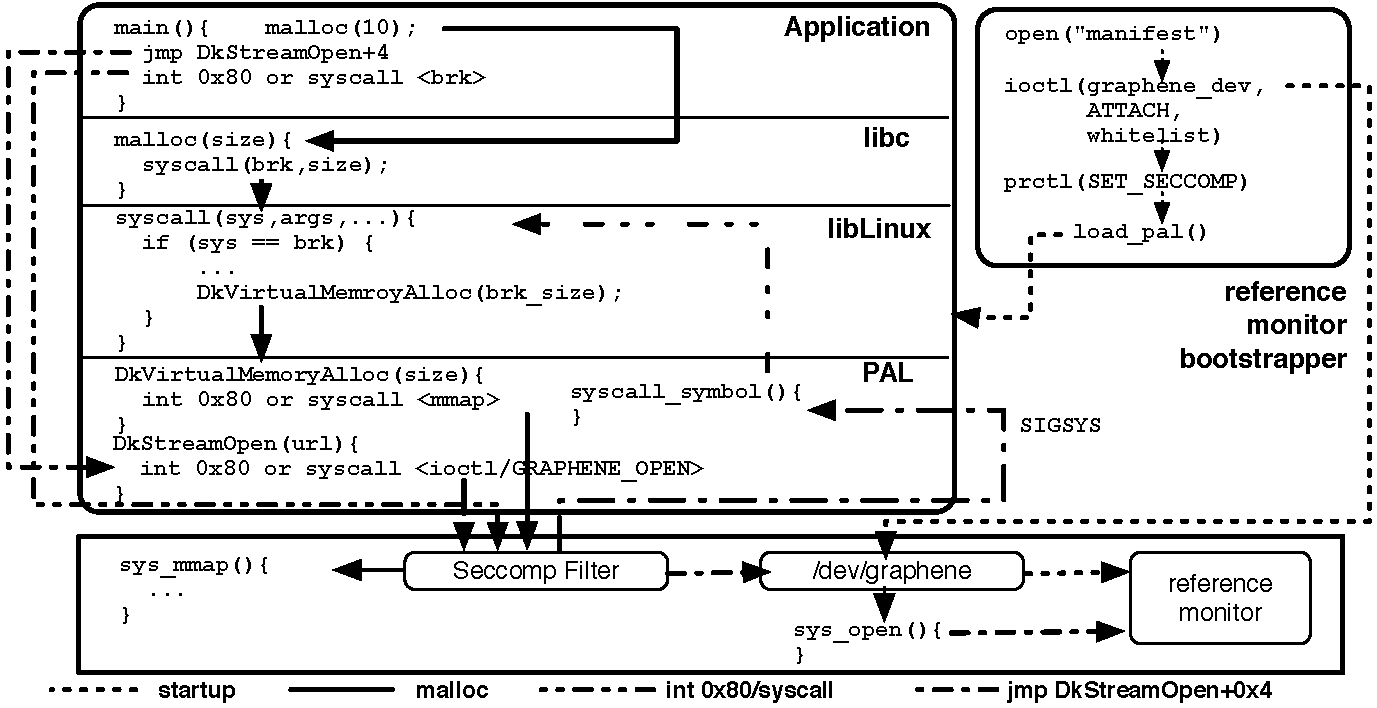
\includegraphics[width=\linewidth]{syscall-redirection.pdf}
\footnotesize
\caption{System call redirection for \thelibos{}.
In the normal case (first line of {\tt main}), {\tt malloc} is invoked causing the invocation of {\tt brk} ({\tt libLinux}) and {\tt mmap} in the \pal{}. In the second line, the application jumps to an address in \pal{}, which is permissible.
Files are accessed through {\tt ioctl} to {\tt /dev/graphene} and checked by reference monitor.
The third line invokes {\tt brk} with an {\tt int} instruction, which is redirected to the {\tt libLinux} function.}
\label{fig:libos:syscall-redirection}
\end{figure}


\graphene{} modifies several \glibc{} libraries with individual purposes,
%When using \graphene{}, an application must be deployed with the modified \libc{} libraries,
including \code{ld.so}, \code{libc.so}, \libpthread{}, and \libdl{}.
\Glibc{} partitions its code into separate libraries to reduce the binary sizes
loaded by each application.
%Despite that \glibc{} has partitioned its code into separate libraries,
\graphene{} only modifies the libraries which contains direct \linuxapis{} (i.e., \assembly{syscall} instructions).
%not every libraries of \glibc{} need to be modified for \linuxapi{} redirection.
%Only \code{libc.so}, \libpthread{}, and \libdl{} have included \code{syscall} instructions,
%and thus have to be modified for \graphene{}.
Other \libc{} libraries, such as \code{libm.so},
never directly invoke \linuxapis{} and only rely on 
existing \libc{} functions;
therefore, \graphene{} leaves \code{libm.so} and other similar \libc{} libraries unmodified.



\paragraph{Hard-coded \linuxapis{}.}
A static binary, or a platform-dependent application, may contain hard-coded \assembly{syscall} instructions
that cannot be redirected by a modified \libc{}.
Some application developers choose to statically link an executable against \libc{},
as a static binary with hard-coded \linuxapis{}. %\code{syscall} instructions.
Other application developers may program an application---usually a language runtime (e.g., go runtime) or system software (e.g., \projname{busybox})---with assembly code that directly invokes
platform-depenedent,
rare \linuxapis{} that are not wrapped by \libc{} functions.
%one of the \linuxapi{} wrappers in \libc{}, or \funcname{syscall}.
%As a result, a ELF binary may contain hard-coded \assembly{syscall} instructions.
%Either way leads to hard-coding \code{syscall} instructions in the ELF binaries.
Because modified \glibc{} does not redirect hard-coded \linuxapis{},
the \linuxapis{}
trigger context-switching into the host kernel,
causing security and compatibility issues as
exposing unauthorized, or unsynchronized host resources and states to the application.


As a solution,
\thelibos{} depends on host-level \linuxapi{} restriction to redirect hard-coded \linuxapis{}.
%to prevent \linuxapis{} from anywhere other than a PAL.
A direct \linuxapi{} traps into the host kernel,
unless the host has virtualized the interrupt handler to the \libos{}.
\graphene{} depends on each host to
detect unauthorized \linuxapis{} either from a wrong code location or with an unexpected \linuxapi{} number.
On Linux or a similar OS, the PAL can install a \linuxapi{} filter,
such as SECCOMP filter~\cite{seccomp}.
On some architecture, there are architectural limitation;
for example, SGX forbids \linuxapis{} inside an enclave and triggers an exception for an in-enclave \linuxapi{}.
%\code{syscall} instructions
%(e.g., SGX restriction).
%The details of the \linuxapi{} restriction mechanisms are discussed in
%\fixme{update labels}
%Section~\ref{sec:linux:syscall} and Section~\ref{sec:sgx:syscall}.
\thehostabi{} specifies that the host captures unauthorizes \linuxapis{}
and redirects to an exception handler (set up by \palcall{ExceptionSetHandler}).
%If a binary makes an illegal \linuxapi{},
%the host-level \linuxapi{} restriction will trigger an \code{ILLEGAL} exception
%at \thehostabi{},
%and thus the \linuxapi{} is redirected by an exception handler
%assigned by \thelibos{}.
The exception handler 
retrieves the \linuxapi{} number and arguments
from the saved context,
runs the \linuxapi{} handler,
and eventually pushes the return value back to the saved context. %\code{RAX} register.


Redirecting \linuxapis{} based on exceptions
can be expensive,
due to the overhead of context-switching between the host and guest.
Whenever an application invokes a direct \linuxapi{},
it traps into the host kernel, and then returns to the \libos{} to handle the \linuxapi{}.
Therefore, the process of redirecting a \linuxapi{} includes at least two times of context-switching, which can take up to microseconds.
To bypass the overhead,
\thelibos{} can 
rewrite the binary at run-time to redirect the hard-coded \linuxapis{};
%use {\bf binary translation} to modify the hard-coded \code{syscall} instructions;
\thelibos{} can
either scan-and-rewrites the whole binary at loading time,
or rewrites a single \assembly{SYSCALL} instruction in the exception handler.
%binary translation
%can be triggered when a host-level exception is raised
%for an illegal \linuxapi{},
%to optimize consecutive \linuxapi{} invocation at the same location.
%\thelibos{} can also perform a full scan in application binaries
%to spot and modify hard-code \code{syscall} instructions.
\graphene{} leaves the implementation of binary rewriting
as future work.



%\section{Automatic Partitioning of JAVA Applications}
\label{sec:partitioning}
\sysname{} reduces the TCB of a security critical 
application by automatically partitioning the 
application into trusted and untrusted parts. It is not 
easy for a novice developer to find the right 
partitioning boundary. As a result, the developer may 
include classes, which are not necessary for operation, 
in the trusted part. These extra classes may expose new 
attack vectors, reducing the security of the enclave. 
\sysname{} provides an enclave image utility to help 
the developer partition the code with minimum effort. 
The developer only needs to identify the classes that 
represent the secure objects.

The enclave image utility calculates the transitive 
closure of dependencies of the secure object classes.
The tool traverses all the imported classes by secure 
classes and marks them as secure too. The tool keeps 
traversing the newly added secure classes until there 
is no new class to be marked secure. It not only 
follows the user-defined classes but also the system 
classes to create a list of all the secure classes.

The utility then replaces the references of secure classes in the untrusted part with proxy stubs to make a remote method call instead of direct method invocation. The tool uses Phosphor information  flow tracking library to instrument the secure classes so that the information flow can be tracked at runtime as explained in Section ~\ref{sec:info-leak}. The output of the tool is an instrumented secure classes JAR and another JAR containing untrusted code with proxy stubs.

The enclave image tool then packages the Graphene LibOS, JVM, JNI, and the instrumented trusted JAR together, and generates the enclave object by cryptographically signing the package using its private key and \fixmebj{XX} algorithm. The untrusted JAR and the enclave object are deployed together in the cloud machine with \sgx{} capability. 

Thus, the automatic partition tool reduces the attack vectors exposed in the enclave, and removes the burden of the developer to create the partition boundary by finding the entry/exit points. This enforces a strict smallest possible TCB for the secure application.

%\papersection{Security isolation}
\label{sec:linux:security}

\issuedone{1.1.d}{Describe the security isolation story for Linux hosts}
\graphene{} separates OS features from security isolation.
This section explains the Linux host design for isolating mutually untrusting applications, with a reduced attack surface for protecting Linux kernels.
The discussion starts with the security guarantees and threat model, followed by the technical details of security isolation on a Linux host.



\papersubsection{Goals and threat model}

The security isolation model of \graphene{} ensures that mutually-untrusting applications cannot interfere with each other.
A goal of \graphene{} is to provide security isolation with comparable strength as
running applications in separate VMs.
When running two unrelated applications on the same machine,
the security requirement
of the OS involves not only blocking unauthorized access under normal circumstance,
but also preventing an application
from maliciously exploiting OS vulnerabilities to attack the other application.
Because a modern OS, such as Linux or \win{}, contains a rich of features and APIs,
it is difficult to eliminate OS vulnerabilities
or even just to verify whether an OS contains any vulnerabilities. 
A Linux container~\cite{lxc}
does provide a separate OS view for each application,
but still relies on the correctness of the whole Linux kernel to enforce security isolation.
On the other hand, a VM or a \libos{}
isolates the whole OS kernel or a part of the kernel in an unprivileged guest space
for each application.
The security isolation model prevents
any vulnerabilities inside the VM or the \libos{} from compromising the host kernel and other applications.



\graphene{} enforces security isolation %between applications
by separating 
backward-compatible OS features from security mechanisms.
A Linux kernel exports a wide range of system calls,
either as a legacy of previous kernels or as new programmability features. % of newer kernels.
By implementing OS features in a \libos{},
\graphene{} reduces the attack surface of a Linux kernel
to a small amount of system call corner cases.
%to implement \thehostabi{}.
%If a machine only runs applications in \graphene{},
%a Linux developer can try to carve out a minimal Linux kernel, containing only features needed by the Linux PAL.
A reduced attack surface
eliminates majority of execution paths inside a Linux kernel in which a malicious application can explore for vulnerabilities.
The complexity of Linux features and APIs exported by a \libos{} is unrelated with the attack surface of the host kernel,
unless the \libos{} asks for additional \hostapis{}.
A Linux developer can even carve out a minimal Linux kernel with only the features needed by the Linux PAL,
similar to shrinking a Linux kernel to a microkernel.
Otherwise, \graphene{} depends on the host security mechanisms to restrict a \libos{} from accessing unauthorized system calls and resources upon an unmodified Linux kernel.





The Linux PAL installs a {\bf system call filter} and a {\bf reference monitor}
for restricting the system calls, files, RPC streams, and network addresses
accessed by a \picoproc{}.
The Linux PAL requires \hostsyscallnum{} system calls in total
for implementing both required and optional \hostapis{}.
A system call filter, such as the Linux \seccomp{} filter~\cite{seccomp},
can restrict the system call access of an application
to only a small subset of all the system calls, with additional constraints on the parameters and optional flags permitted for each system call.
%The system call filter
%forbids an application from invoking any system calls
%that will interfere other \picoproc{} or increase the risk of exploitation in the host kernel.
A reference monitor further examines the arguments of permitted system calls to restrict the host resources accessed by an application, based on security policies configured in a manifest file~\cite{hunt07rethink}.
The system call filter and the reference monitor
significantly limit the ability of an untrusted \graphene{} \picoproc{} to interfere with the rest of the system,
preventing the risk of exposing any unknown vulnerabilities
on a kernel path never exercised by the system call footprint of \graphene{}.



\graphene{} contributes a multi-process security model 
based on a {\bf sandbox},
or a set of mutually-trusting \picoprocs{} running inside an isolated container.
The reference monitor permits picoprocesses within the same sandbox
to communicate over RPC streams,
allowing the \libos{} to share and coordinate any states
to create an unified OS view.
If two \picoprocs{} belong to different sandboxes,
the reference monitor will block any attempt of connecting RPC streams
between the \picoprocs{}
The access control over RPC streams
enforces an all-or-nothing security isolation model:
either two \picoprocs{} are in the same sandbox and share all the \libos{} states; or they are separated in two sandboxes and share nothing.
Even though the \libos{} instance can span its state across multiple \picoprocs{},
a host kernel needs not to examine the accesses to shared \libos{} states, but still enforces security isolation between sandboxes.




Files and network addresses
are the only host resources allowed to be shared across sandboxes,
using well-studied, explicit rules.
For sharing files, the reference monitor restricts the file access of a \picoproc{}
within a few host file or directories,
creating a restricted view of the local file system
(close to Plan 9's unionized file system views~\cite{pike90plan9}).
The file rules
in a manifest are similar to the policies of a {\bf AppArmor profile}~\cite{apparmor};
for each permitted file or directory,
a developer specifies the URI prefix and the permitted access type, either as read-only or readable-writable. %, within the target file or directory.
For sharing network addresses,
the reference monitor restricts a \picoproc{} from connecting through a local address or connecting to a remote address,
using {\bf iptables-like firewall rules}~\cite{iptablesman}.
Each network rule in a manifest
specifies the local or remote IP address and port range that a \picoproc{} is permitted to bind or connect a network socket.
The rules in a manifest file
specify a minimal list of files and network addresses that a \picoproc{} needs to access, and are largely based on existing security policies (e.g., AppArmor profiles, firewall rules).





\paragraph{Threat model (details).}
When running on a normal Linux host (without \sgx{} or other security hardware), \graphene{} assumes a trusted host kernel and reference monitor.
All the components inside the kernel space, including the \code{gipc} kernel module for bulk IPC, and the reference monitor,
are fully trusted by the other parts of the host kernel and the \graphene{} \picoprocs{}.
%which mediates all system calls with effects outside of a picoprocess's address space,
%such as file {\tt open} or network socket {\tt bind} or {\tt connect}.
On the other hand,
the host Linux kernel does not trust the \picoproc{}, including the Linux PAL, a \thelibos{} instance, \glibc{}, and the application.
The system call filter and reference monitor
initialized before an application starts running
defend the whole host kernel from malicious system calls invoked by a \picoproc{}.



All the components running within a \picoproc{}, including the Linux PAL, the \libos{} (\thelibos{}), \glibc{} libraries, and the application,
mutually trust each other. %, because all these components
%execute in the same guest address space.
Without internal sandboxing, the Linux PAL or \thelibos{}
cannot protect its internal states or control flows from an application.
Although some scenarios might require protecting the PAL or \thelibos{}
from the application,
\graphene{} only restricts the adversary
within a \picoproc{};
in other word, an adversary
only compromises the \libos{} in the same \picoproc{},
but can never interfere the host kernel 
or other unrelated \picoprocs{}.



For a multi-process application,
\graphene{} assumes that the \picoprocs{} 
%launched by the same application instance
running inside the same sandbox
trust each other and that all untrusted code run in sandboxed \picoprocs{}.
\graphene{} assumes the adversary can run arbitrary code inside
one or multiple \picoprocs within a sandbox.
The adversary can exploit any vulnerabilities in the \libos{}
or IPC protocol,
to propagate the attack to other \picoprocs{}.
\graphene{} ensures that
the adversary cannot interfere with any victim \picoprocs{}
in a separate sandbox.
A sandbox strictly isolates the coordination of \thelibos{} instances;
%if the only shared kernel abstractions are byte streams and files, 
the reference monitor ensures
that there is no writable intersection between sandboxes, so that
the adversary cannot interfere with any victim \picoprocs{}.


%%% The only processes allowed to run as standard kernel processes (non-\graphene{}) 
%%% are the reference monitor and
%%% system administration utilities that need more kernel interfaces than the \pal{} ABI provides.
%%% Ensuring that a collaborating picoprocess correctly implements
%%% some function (such as receiving a signal),
%%% as well as preventing exploitation of vulnerabilities in picoprocesses
%%% are beyond the scope of this work.

\graphene{} reduces the attack surface of the host Linux kernel, but does not change the trusted computing base; however, reducing the effective system call table size of a \picoproc{} does facilitate adoption of a smaller host kernel.
This thesis leaves the creation of a smaller host kernel for future work.

\papersubsection{System call restriction}
\label{sec:linux:security:syscall-restriction}


\graphene{} reduces the host ABI to \palcallnum{} calls
and the Linux system call footprint to \hostsyscallnum{} system calls.
To reduce the effective attack surface to a Linux host,
the Linux host restricts a \picoproc{} from accessing any system calls that are not part of the ordinary footprint of a Linux PAL.
The system call restriction on Linux focuses on blocking most of the system calls
that interferes with other processes.
The remaining permitted system calls with external effects are checked by 
the reference monitor (see Section~\ref{sec:linux:security:ref-monitor}).
 
%% dp: Meh
%%% Any picoprocess implementation 
%%% must restrict access to the host system call table,
%%% generally by blocking system calls in the host kernel~\cite{porter11drawbridge}
%%% or using {\tt ptrace}~\cite{xax}.


%The \pal{} is a host-provided library which implements \palcalls{} generic kernel ABIs,
%implemented using 
%These native system calls include {\tt ioctl} with 5 opcodes exclusively used by \graphene{} kernel extensions.

%This section describes how we adapt recent Linux sandboxing techniques 
%to \graphene{}.


%all allowed system calls with potentially external effects.

%%% For instance, an attempt to open a file will be checked by the reference monitor
%%% to see if the file is included in the sandbox definition, specified in the manifest
%%% with required permissions.
%%% Once the file handle is open, the \pal{} is then allowed to issue an {\tt mmap} or {\tt read}
%%% on the handle, as this operation can only affect the picoprocess address space
%%% or  file, which was already checked.

%Because the \pal{} is in the same address space as the application code, it is not
%trusted to enforce any security policies, and our threat model assumes that
%the \pal{} can be compromised by the adversary.
%Thus, the host kernel 
%only permits system calls that appear in the \pal{}'s source code and, through the reference monitor, further inspects calls that can have external effects.

%\begin{figure}[t!]
%\centering
%\includegraphics[width=\linewidth]{syscall-restriction.pdf}
%\footnotesize
%\caption[System call restriction approach in sysname{}]
%{System call restriction approach. The reference monitor loads policies into the LSM at startup.  A \graphene{} application requests OS services in three different ways. 
%In the normal case (first line of {\tt main}), {\tt malloc} is invoked causing the invocation of {\tt brk} ({\tt libLinux}) and {\tt mmap} in the \pal{}. In the second line, the application jumps to an address in \pal{}, which is permissible.
%Files are accessed through {\tt ioctl} to {\tt /dev/graphene} and checked by reference monitor.
%The third line invokes {\tt brk} with an {\tt int} instruction, which is redirected to the {\tt libLinux} function.}
%\label{fig:graphene:syscall-restriction}
%\end{figure}



\issuedone{1.3.d}{Extend the discussion of \seccomp{} filter}
\graphene{} restricts the host system calls 
using a \seccomp{} %(SECure COMPuting)
filter~\cite{seccomp}, a feature introduced in Linux 2.6.12.
% a recent Linux system call filtering mechanism, called 
A \seccomp{} filter allows a Linux process to install an immutable Berkeley Packet Filter (BPF) program
that specifies allowed system calls, as well as specifies
the consequence of invoking certain system calls, such as creating a \code{ptrace} event or raising a \code{SIGSYS} signal.
The BPF grammar is rich enough to filter scalar argument values,
such as only permitting specific opcodes for \syscall{ioctl},
as well as filter certain register values, such as blocking system calls from program counters (i.e., \code{RIP} register values) outside of the Linux PAL.
%This feature is particularly salient in the case of {\tt ioctl},
%where the \pal{} uses 5 out of over 400 opcodes for our bulk IPC module and sandbox creation;
%our BPF rules will block any other {\tt ioctl} opcode.
The current \seccomp{} filter installed by the Linux PAL contains \seccomplines{} lines of straightforward BPF macros.  %Experiments show that adding more precise argument checks has no significant impact on system call latency.
Once a \seccomp{} filter is installed in a process,
the filter intermediates
every system calls from the process and its future children, and guarantees the processes can never bypass the restriction.
The Linux PAL uses \code{SIGSYS} signals to capture rejected system calls,
and can either terminate the whole application or
redirect the system call to \thelibos{}.
The consecutive steps of system call redirection are described in Section~\ref{sec:libos:syscall-redirection}.



Developing a \seccomp{} filter presents several technical challenges.
First, a filter must restrict consecutive \picoprocs{}
to install a new filter the reverts the system call restriction.
%A \seccomp{} filter is installed using the \syscall{prctl} system call, so
Blocking the \syscall{prctl} system call in a \seccomp{} filter will prevent further installation of \seccomp{} filters.
Second, the BPF grammar can only filter certain values or ranges of a register.
The filter needs to
ensure that only the Linux PAL can invoke system calls;
however,
for satisfying the dynamic loading behavior of \thehostabi{},
the Linux PAL
is built as a shared library loaded at an address randomized by the Linux ASLR (Address Space Layout Randomization) feature.
If a filter only permits a specific range of program counters,
a child \picoproc{}
will load the Linux PAL at another randomized address,
and the inherited filter will restrict the child \picoproc{} to invoke any system calls.
The Linux PAL introduces a small, initial loader
loaded at a fixed address
within each \picoproc{} and permitted to invoke system calls.
Finally, a \seccomp{} filter
cannot check a string argument, such as a file path for \syscall{open} or a network address for \syscall{bind}.
Checking a string argument requires
involves reading user memory of unknown sizes and string comparison, and the BPF grammar only allows checking an argument arithmetically.
Filtering permitted file paths and network addresses
must rely on a trusted reference monitor (see Section~\ref{sec:linux:security:ref-monitor}).
%In order to avoid the overhead of trapping to the reference monitor on 
%every use of {\tt open}, {\tt stat}, {\tt bind} or {\tt connect} system calls, we instead 
%force picoprocess to only use {\tt ioctl} system call to \graphene{} special device ({\tt /dev/graphene}) as alternative interface these system calls. Direct access to these system calls are banned by seccomp filter.
%extend AppArmor~\cite{apparmor} 
%to enforce file system isolation in the kernel.



The \seccomp{} filter blocks  unauthorized system calls
from anywhere inside a \picoproc{}.
Even if none of the application binaries contains any \assembly{syscall} or \assembly{int \$80} instruction,
a piece of malicious application code can always bypass the Linux PAL
to invoke unauthorized system calls.
The application code can simply
jump to a \assembly{syscall} instruction inside the Linux PAL,
or corrupt a returned address on the current stack to launch a ROP (return-oriented programming) attack.
Even if the Linux PAL is hidden or isolated from the application,
an adversary can always leverage a gadget, a byte sequence that resembles the target instruction, within an executable or a library.
Therefore, the \seccomp{} enforces both program-counter-based 
and argument-based restrictions
to block unauthorized system calls from both the Linux PAL and the rest of \picoproc{}.


%In order to reduce the impact of bugs in the reference monitor,
%the reference monitor itself runs with a \seccomp{} filter, blocking unexpected system calls.


\paragraph{Security implications.}
Using an existing system call restriction mechanism like \seccomp{},
\graphene{} limits the ability of an untrusted application to attack a Linux kernel.
Ideally, since \thelibos{} only requires \thehostabi{},
\graphene{} can adopt a modified Linux kernel
that only exports \palcallnum{} \hostapis{} to each \picoproc{}.
%However, as a usability feature, \graphene{} runs \graphene{} on an unmodified Linux kernel using a Linux PAL to translate among host interfaces.
The \seccomp{} filter instead isolates a \picoproc{} on an unmodified Linux kernel,
with a reduced attack surface 
comparable to only exporting \thehostabi{}.
%The filter only permits \hostsyscallnum{} system calls with specific flags and opcodes
%required by the Linux PAL.
According to the principle of least privilege,
each component or layer in a system should only be granted access to a minimal amount of resources or abstractions
required for performing the expected tasks.
The \seccomp{} filter only permits
a minimal amount of system calls with specific flags and opcodes
required by the Linux PAL,
so an untrusted application
can only trigger
a limited amount of execution paths inside the host Linux kernel.
\graphene{} limits
the ability of an untrusted application to explore
known and unknown vulnerabilities
on any kernel execution paths for servicing one of the blocked system calls.



Although a regular Linux process can also leverage a \seccomp{} filter,
\graphene{} makes a major contribution
to reduce the system call footprint of any large-scale application
to a fixed, small system call profile.
Analysis %of applications and libraries
%in the official Ubuntu repositories
shows that the system call  footprint of a large-scale application such as Apache or MySQL can contain more than 100 system calls.
Since \thelibos{} has absorbed the Linux system call table,
running Apache, MySQL, or any other application in \graphene{} leads to at most \hostsyscallnum{} host system calls.
As a system
running a wide range of applications
can exposes a different partial view of the system call table to each application,
\graphene{}
has a static system call profile for all applications,
allowing OS developers to focus
on testing or analyzing a small portion of execution paths and corner cases
of a Linux kernel.
\citet{sun15unpredictability}
proposes sandboxing an uncertain, potentially-malicious application
in \graphene{}
with an unpredictable \thelibos{} implementation.







\paragraph{Static binaries.}
Besides security purposes,
a \seccomp{} filter provides a compatibility feature
for redirecting hard-coded system calls
in a statically-linked application binary.
\graphene{} leverages the \seccomp{} filter to redirect these leaked system calls
back to \thelibos{}. 
The filter contains BPF rules to check if the program counters
invoking the system calls
are parts of the Linux PAL.
The filter blocks system call invoked outside of the Linux PAL
and delivers a \code{SIGSYS} signal
to the PAL signal handler for redirecting the system calls to \thelibos{}.



\papersubsection{Reference monitor}
\label{sec:linux:security:ref-monitor}

The reference monitor on a Linux host
checks the arguments of host system calls for referencing any sharable host resources.
A host system call like \syscall{open}, \syscall{connect}, or \syscall{bind}
specifies a file system path or a network address
for opening a file or network stream and cannot be filtered by a \seccomp{} filter.
The host kernel trusts the reference monitor
to only permit
a list of sharable resources in a \picoproc{},
based on
rules in a manifest file.
Once the reference monitor has permitted the creation of a file or network stream,
consecutive operations on the stream
such as reading or writing data can be trusted
as long as being mediated by one of the permitted system calls.


\begin{figure}
\centering
\begin{lstlisting}
loader.exec = file:/usr/sbin/apache2        # allow loading executable 
loader.preload_libs = file:/graphene/libLinux.so    # loading libLinux
fs.allow_ro.libc = file:/graphene/libc/     # loading modified libc
fs.allow_ro.mods = file:/usr/lib/apache2/modules/   # loading modules
fs.allow_ro.cond = file:/etc/apache2/       # reading configuration
fs.allow_rw.logs = file:/var/log/apache2/   # writing to logs
fs.allow_ro.http_docs = file:/var/www/      # reading website files
net.allow_bind.httpd = 0.0.0.0:80           # binding to local port 80
net.allow_conn.any = 0.0.0.0:1-65535        # allow any connection
\end{lstlisting}
\caption{A example of a manifest file, containing security rules for the reference monitor to permit accessing sharable resources. The manifest file is for running a Apache http server (without php and other language engines).}
\label{fig:linux:manifest-example}
\end{figure}


The reference monitor enforces simple, white-listing rules
based on security mechanisms
already familiarized by users and developers.
Figure~\ref{fig:linux:manifest-example} shows an example of resource access rules
in a manifest.
First, a manifest lists
the URI prefixes of permitted files or directories
of an application,
similar to an AppArmor profile.
The executable (\code{loader.exec}) and the preloaded \libos{} binaries (\code{loader.preload\_libs})
are permitted for read-only access by default.
The reference monitor
simply compares file URIs against each permitted URI prefix
and checks the access types;
unlike many existing security mechanisms in Linux and similar OSes, such as permission bits, Access Control Lists (ACLs), and SELinux labels,
the reference monitor does not retrieve
security policies from file metadata, but obtains the manifest from an out-of-band channel.


Manifest-based security
simplifies the inspection, authentication, and population
of security policies.
An Android application is deployed with a similar manifest,
listing the accessed files and other resources,
which users approve when installing the application.
Developers can authenticate a security policy by signing the content of a manifest.
Moreover, to run an application, a user can choose among multiple manifest files
with different levels of security privileges.



Network rules in a manifest are similar to {\bf iptables firewall rules} for defending a server or a desktop machine.
A network rule specifies a local or remote address
that the application is permitted to bind or connect a network stream.
A local or remote address
can be an IPv4 or IPv6 address (possible to specify an ``any'' address, i.e., \code{0.0.0.0} or \code{[::1]}), combined with a specific port number or range.
When an application creates a network stream,
the reference monitor checks whether the local and remote addresses
match one of the network rules.







%is implemented using {\tt ioctl} system call to a special device {\tt /dev/graphene}.
%A picoprocess is restricted by seccomp filter~\cite{seccomp} to use any {\tt open} or socket {\tt connect} and {\tt bind} system calls.
%It must use the \graphene{} special device to open or create streams,
%so the file paths or network addresses can be checked against the sandbox rules.
%The kernel module as the driver of the \graphene{} special device can coexist with any LSM such as \emph{AppArmor} or \emph{SELinux}.

The reference monitor on a Linux host
is implemented as a Linux Security Module (LSM) extended from the existing AppArmor module.
AppArmor is the default LSM of most Linux distributions,
and a Linux kernel disallows multiple LSMs (e.g., AppArmor, SELinux) to be effective simultaneously.
\graphene{} instruments
a few security hooks of the AppArmor, to add checks for file system paths
and network addresses.
The security checks of the reference monitor are stackable with other host security mechanisms.
For example, if a manifest lists a root-privileged file and the \graphene{} application runs in a unprivileged process,
existing security checks in a Linux kernel
still blocks the file access even though the reference monitor permits the access.
The drawback of the implementation
is that \graphene{} must run on a modified Linux kernel.
Linux kernels do not support loading LSM as a dynamic kernel module.
\graphene{} only replaces
the AppArmor LSM in a Linux kernel; the rest of the Linux kernel remains unchanged.


A trusted security loader initializes the reference monitor
when launching an application in \graphene{}.
When a user launches an application in \graphene{} from the command line,
the first \picoproc{} begins in a new sandbox.
The security loader
reads the manifest file given by the user,
and submits the sandbox rules to the reference monitor.
The reference monitor exports a miscellaneous device called \code{/dev/graphene}
for the security loader to submit sandbox rules using the \syscall{ioctl} system call.
Once the reference monitor
starts a \picoproc{} in a sandbox, neither the first \picoproc{} nor any consecutive \picoprocs{} spawned in the sandbox can ever escape the sandbox or drop the restrictions on certain resources.


\paragraph{Alternative approaches.}
Other approaches can implement the reference monitor without modifying a Linux kernel, with a trade-off of performance or development simplicity.
An approach is to implement the reference monitor as a trusted process receiving \code{ptrace} events from \graphene{} \picoprocs{}.
Using the \syscall{ptrace} system call, this reference monitor can retrieve user memory from the monitored \picoprocs{},
and block the system calls which request for unpermitted resources.
Unfortunately, intercepting every system calls with \code{ptrace} events introduces significant overhead to \hostapis{};
thus, this approach is not ideal for isolating \graphene{} applications on a Linux host.


Another approach is to translate the resource rules in a manifest file
to AppArmor or iptables rules.
As explained in previous paragraph, the file and network rules in a manifest file are similar to the file lists in an AppArmor profile and the firewall rules enforced by iptables.
Instead of implementing a \graphene{}-specific reference monitor,
\graphene{} can convert a manifest file, either statically or dynamically,
to security rules recognized by AppArmor and iptables.
This approach requires no modification
in a Linux kernel, and can benefit from
existing optimizations of AppArmor and iptable. %these security mechanisms.
\graphene{} leaves the integration with AppArmor and iptables for future work.




\paragraph{Dynamic process-specific isolation.}
A child \picoproc{} may either inherit its parent's sandbox, 
or start in a new sandbox,
by either specifying a flag to \palcall{ProcessCreate} or calling the sandboxing \hostapi{}, \palcall{SandboxSetPolicy}.
A new sandbox may obtain a subset of the original file system view,
but can never request access to new regions of the 
host file system. 
%The restrictive policy enforced on the child will be written in a new manifest file generated by the parent, and the policy will be checked by the reference monitor.
If a child \picoproc{} voluntarily moves itself to a new sandbox
using \palcall{SandboxSetPolicy},
the Linux PAL issue another \syscall{ioctl} call to \code{/dev/graphene}
to dynamically detach
the \picoproc{}
from the parent's sandbox and update sandbox rules. The reference monitor
closes existing RPC streams and prevents RPC stream creation 
across sandboxes.
%among picoprocesses
%that are not in the same sandbox.
%and restricts external connections to remote URIs according to firewall rules in the manifest.
When a process detaches from a sandbox,
the reference monitor effectively splits the original sandbox
by closing any RPC streams that could bridge the two sandboxes.


\begin{comment}
We hasten to note that program counter filtering
is only provided for backwards compatibility, not security.
An attacker can compromise the \pal{}, so system policies are enforced
externally by the reference monitor.


Dynamically redirecting system calls to {\tt libLinux} is 
less efficient than dynamically linking against
the \graphene{} libc or statically compiling {\tt libLinux} into the application.
The overhead of dynamic redirection comes from 
transferring control to the kernel, then back to 
the \pal{}, and then to {\tt libLinux}.
We leave exploration of more efficient alternatives for future work,
such as redirecting the hardware system call table to {\tt libLinux}
on a host system like Dune~\cite{belay12dune},
or dynamically rewriting parts of the static binary~\cite{hunt99detours}.
\end{comment}

%\paragraph{Example.}
%Figure~\ref{fig:graphene:syscall-restriction} illustrates three possible situations. 
%%% An unmodified Linux application is dynamically linked against the 
%%% \graphene{} {\tt libc}, 
%%% which then dynamically links its system calls from {\tt libLinux},
%%% which in turn links in the host kernel ABI from the \pal{}.
%%% The application requests OS functionality in three ways.
%An unmodified application first invokes the {\tt libc} function {\tt malloc}, which issues 
%a {\tt brk} system call to {\tt libLinux}, which requests memory 
%from the host via a {\tt Dk\-Virtual\-Memory\-Alloc} \pal{} call,
%which ultimately issues an {\tt mmap} host system call.
%The {\tt mmap} host system call is allowed by seccomp because it only 
%affects the picoprocess's address space.
%The second line of the application jumps to the \pal{} instruction that issues
%an {\tt open} system call.
%From a security perspective, this is permissible,
%as it is isomorphic to \pal{} functionality.
%In practice, this could cause
%corruption of {\tt libLinux} or application data structures,
%but the only harm is to the application itself. 
%Because this system call involves the file system, the reference monitor LSM first checks if the file to be opened is included in the sandbox definition (manifest) before allowing  the {\tt open} system call in the kernel.  
%Finally, the application uses inline assembly to issue a {\tt brk} system call;
%%in an attempt to obtain I/O port privilege; 
%because this system call was not issued by the \pal{},
%seccomp will redirect this call back to the \pal{},
%which then calls the {\tt libLinux} implementation.


Sandbox creation in \graphene{} can provide
more options than virtualization, to reflect the security policy of applications at any timing,
in the granularity of picoprocess. 
A picoprocess can voluntarily detach itself from the current sandbox, dropping its privileges,
after finishing security-sensitive operations.
If a picoprocess decides one of its children is not trustworthy, it may also start the child under a restricted manifest,
or promptly shut down RPC streams to stop sharing OS states.
The picoprocess that moves to a separate sandbox will have a restrictive view of the filesystem, and no coordination with the previous sandboxes.
Section~\ref{sec:eval:graphene} describes an experiment that improves security isolation of Apache http server without sacrificing functionality.



%We add a \pal{} call which
%permits a picoprocess to request that it be moved into a new sandbox.
%This call, as well as file system path checks, are implemented
%as extensions to the  AppArmor LSM~\cite{apparmor}.
%%We modify \sandboxmodlines{} lines in the
%%to implement this call,
%The new sandbox call closes any open stream handles that cross sandbox boundaries;
%mediate path lookups;
%and create a new broadcast stream for multi-process
% coordination (\S\ref{sec:graphene:namespaces:blocks}).
%%The reference monitor also interposes on this call so that it can 
%%mediate future stream creation.

%To securely apply seccomp filtering we leveraged the fact that all
%\graphene{} processes have the same parent and also the new
%{\tt NO\_NEW\_PRIVS} bit introduced for Linux processes starting kernel
%version 3.5. This bit can be set by any process, is inherited across
%{\tt fork}, {\tt clone}, and {\tt execve}, and cannot be unset by
%children processes. Thus, we set the {\tt NO\_NEW\_PRIVS} bit in the initial
%\graphene{} process and apply seccomp filters allowing only system calls
%with corresponding functions in the \pal{}. As a result all \graphene{}
%processes will inherit the filters and cannot relax or bypass it.



%which reduces the kernel
%system call API surface to user-level processes. This mechanism allows
%a process to specify a whitelist filter for system calls, which is
%implemented as a Berkeley Packet Filter (BPF) program. The invocation
%of a disallowed system call causes the application to throw a {\tt SIGSYS}
%signal, which can be caught by a registered handler provided by the
%application. In \graphene{} we registered this handler at the \pal{}.


%\graphene{} applications rely on an OS loaded as a library to request
%system services. As most of traditional applications, \graphene{}
%processes do not normally issue system calls directly: they invoke
%wrapper functions from a \graphene{}-compliant version of libc, which
%allows for portability, security (parameters are limited and checked)
%and easiness of programming. However, while standard libc functions
%directly invoke the kernel system call themselves, our modified
%version of libc wrappers invoke functions from another library which
%represents the OS, libLinux (Figure \ref{fig:graphene:syscall-restriction}). A
%\graphene{} application can access all necessary system functionality
%through libLinux, which invokes corresponding system call functions at
%the \pal{}, also loaded as a library with a
%\graphene{} process. The \pal{} is the layer responsible for directly
%invoking system calls at the kernel. As discussed in \S\ref{sec:graphene:impl} the \pal{} provides \graphene{} applications with a
%subset of the kernel system call interface.\graphene{} applications rely
%on an OS loaded as a library to request system services.
%
%Even though we expect most of \graphene{} applications to leverage libc
%wrappers, we need to address applications that need to invoke system
%calls directly. Applications might need to bypass a library such as
%libc because some needed wrappers are not provided (there are no
%wrappers in libc for module and NUMA related system calls), or the
%wrapper does not meet the programmer’s needs. \graphene{} applications
%that need to perform direct invocation of system calls run unmodified
%as long as the system calls invoked are provided by the libos{l{}. We
%do not consider this a security violation; even though the application
%would be risking not functioning according to the libosaradigm for
%bypassing the \pal{}, all potential damage would be confined in the
%misbehaving application itself.  However, we do not allow the direct
%invocation of a system call that does not have a corresponding
%function in the libosnd \pal{}. In Figure \ref{fig:graphene:syscall-restriction}
%we illustrate these three situations. We have a \graphene{} application
%loaded with three libraries: a \graphene{}-compliant libc, libLinux
%representing the library OS with functions for a selected number of
%system calls, and the \pal{} which actually invokes host kernel system
%calls. The illustrated application requests three different types of
%OS functionality. It first invokes a function from libc, then it
%directly invokes a system call whose functionality is provided by the
%\pal{}, and third it attempts to directly invoke a system call not
%present in the \pal{}, which is not allowed by \graphene{}.

%We enforce system call restriction by leveraging seccomp Linux system
%call filtering mechanism~\cite{seccomp}, which reduces the kernel
%system call API surface to user-level processes. This mechanism allows
%a process to specify a whitelist filter for system calls, which is
%implemented as a Berkeley Packet Filter (BPF) program. The invocation
%of a disallowed system call causes the application to throw a {\tt SIGSYS}
%signal, which can be caught by a registered handler provided by the
%application. In \graphene{} we registered this handler at the \pal{}.
%
%To securely apply seccomp filtering we leveraged the fact that all
%\graphene{} processes have the same parent and also the new
%{\tt NO\_NEW\_PRIVS} bit introduced for Linux processes starting kernel
%version 3.5. This bit can be set by any process, is inherited across
%{\tt fork}, {\tt clone}, and {\tt execve}, and cannot be unset by
%children processes. Thus, we set the {\tt NO\_NEW\_PRIVS} bit in the initial
%\graphene{} process and apply seccomp filters allowing only system calls
%with corresponding functions in the \pal{}. As a result all \graphene{}
%processes will inherit the filters and cannot relax or bypass it.


%\begin{figure}
%\begin{centering}
%\includegraphics[width=2.0in\textwidth]{figures/syscall_restriction.png}
%\footnotesize
%\caption{System call restriction approach. \graphene{} application requesting OS services. The {\tt printf} function is handled by a wrapper function at our modified version of libc., which invoked a corresponding syscall function at libLinux, the library OS.This function invokes a system call function at the \pal{}, which actually invokes kernel system calls. The application also directly invokes two system calls and the last invocation is prohibited.
%\label{fig:syscall_restriction}
%\end{centering}
%\end{figure}

%\end{comment}

%\papersection{Seamless Provisioning of Secure Objects and Classes}
\label{sec:provisioning}

%\section{Framework Implementation}
\label{sec:implementation}

In this section we describe the design of \sysname{}.
\sysname{} adds language support in \java{} virtual machines to
create and execute partitioned applications in enclaves.

\subsection{Partitioned \java{} Execution}

To executed partitioned applications,
\sysname{} creates two worlds of \java{} execution,
one in an enclave and one outside the enclave,
to execute code at different security levels.
Each world contains an individual \java{} vM.
We allow only classes that are part of a signed enclave images to
be executed inside the enclave,
and all the other classes of the application
must run outside the enclave and access the secured classes through
an interface exported by the enclave.

Using \java{} language to implement enclaves
has the benefit of minimizing the development or porting cost.
Consider partitioning a native application for enclaves.
There are two primary sources of development or porting cost:
Separating the security-sensitive code from all the remaining code,
and designing the interface between the two.
%\java{} classes have huge advantage on fulfilling both goals
%with minimal works, for two reasons:
\java{} classes are well modularized and are natural granularity for partitioning.
Public methods can be exported as
enclave interfaces, with proper type-checking of arguments.

%\sysname{} allows \java{} applications
%to easily model enclave support as part of the language,
%without the awareness of the native interface to architecture.
%To reflect this concept, we have implemented two key principles in the language support:
%\begin{compactenum}
\sysname{} models each enclave as an object,
both inside and outside the enclave.
The object is used to access enclave information and features,
such as retrieving security attestation.
Instantiating and interfacing with the isolated classes
in enclaves is transparent to the untrusted part of application,
except the first instantiation.

%For the untrusted side of an application, both the enclave itself and
%the classes isolated in the enclaves
%are encapsulated as black boxes, to which the application
%can request for isolated execution seamlessly.
%These objects can be passed as parameters to other methods,
%or even overrode to extend their functionalities.

\begin{figure}[t!]
\vspace{-0.1in}
\centering
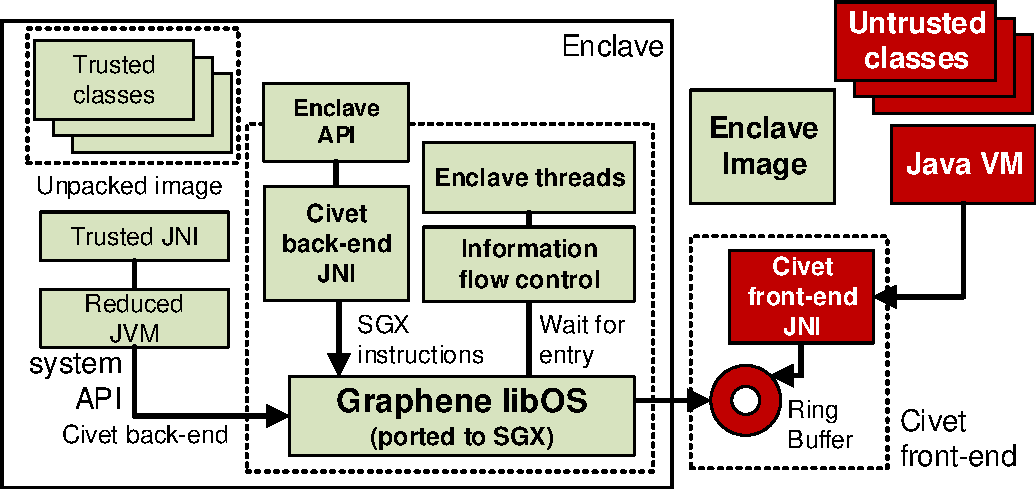
\includegraphics[width=3in]{civet-structure.pdf}
\vspace{-10pt}
\caption{\sysname{} framework overview. \sysname{} creates two worlds for an partitioned \java{} application, each with an individual JVM. The JVM in the enclave is ported using Graphene library OS. Untrusted classes can invoke methods of trusted classes through proxy objects, which will transparently access the enclave interface, through serialization and deserialization over an ring buffer accessed by both untrusted JVM and trust JVM. }
\label{fig:overview}
\end{figure}

\paragraph{Framework overview.} Figure ~\ref{fig:overview} shows the design and 
components of ~\sysname{} infrastructure.
All supporting classes to be isolated in the enclave
are packed into a JAR package --- an enclave image ---
and signed using a key given by the developers.
The untrusted side of the application initializes the enclave
using the enclave image JAR,
and starts to instantiate objects inside the enclave.
For each objects in the enclave, \sysname{} create a {\em proxy object} outside the enclave,
to access the interface exported from the enclave.
%and to represent the isolated objects to the rest of world.

The JVM running inside the enclave is a \jvmname{} VM
ported with the libOS-based programming model, using Graphene library OS.
Proxying isolated objects are handled through JNI in the untrusted JVM,
to access the low-level enclave interfaces.
To invocation of methods on the proxy objects are communicated
through a {\em ring buffer} outside the enclave memory,
accessible by both the enclave and the untrusted application.
The object ID, name of the invoking method, and all parameters are
serialized into binary forms and passed through the ring buffer.
In the enclave, one or more worker threads, initialized by the trusted JVM,
will poll the ring buffer,
accept the invocation requests,
de-serialize the parameters, invoke the method,
and return the result through the ring buffer.

%\begin{figure}[t!]
%\footnotesize
%\noindent
%\begin{minipage}[t]{.38\linewidth}
%\begin{lstlisting}[title=Isolated class,frame=none]
%class Secured {
%  Object run(
%    String args[]
%  ) {
%    ...
%  }
%}
%\end{lstlisting}
%\end{minipage}\hfill
%\begin{minipage}[t]{.54\linewidth}
%\begin{lstlisting}[title=Untrusted class,frame=none]
%class Untrusted {
%  static void main(
%    String[] args) {
%    Enclave e =
%      new Enclave(
%        "enclave.jar");
%    Secured o =
%      e.createInstance(
%        Secured.class);
%    Object r =
%      o.run(args);
%  }
%}
%\end{lstlisting}
%\end{minipage}
%\vspace{-10pt}
%\caption{Example code for using \sysname{} to interact with enclaves. Untrusted classes can use class {\tt Enclave} to create an enclave for a signed image JAR, and instantiate isolated object in the enclave. Invocation of methods of isolated objects will be proxied and forwarded into the enclave.}
%\label{fig:enclave-example}
%\end{figure}

Figure~\ref{fig:enclave-example} shows a code snippet that exercises such a framework.
The instance of class {\tt Enclave} represents the enclave created with
the given image JAR,
and is used to instantiated other isolated objects in the enclave.
Once isolated objects are instantiated,
\sysname{} also creates proxy objects outside the enclave.
All proxy objects belong to subclasses of the original classes,
so they can be casted to the superclasses
and passed around the untrusted application as arguments to other methods.

\paragraph{Limitations.}
Due to the limitations of \java{} class proxying,
untrusted classes cannot transparently invoke static methods
of isolated classes,
due to the ambiguity of which classes shall be accessed.
Also, enclave cannot execute any classes
that are not part of the enclave image JAR.
If untrusted classes passed a object
as the argument to an method of isolated classes,
and the class of the passed object is not part of the enclave image,
the framework will throw a ``Class Not Found'' exception.

\paragraph{Security Implications.}
The primary security implication of such a language support is to
improve {\em usability} of the security hardware.
By providing wrappers for security features and interfaces of an enclave,
developers can easily adopt enclaves into their programming models,
or override existing classes to leverage the hardware.
Because interaction with enclaves are mostly transparent
except the instantiation of first isolated objects,
developers need not to extensively modify existing code,
or constantly be aware of enclave interaction.
Yet all instantiated isolated objects will stay inside the enclave,
regardless of any further method invocation,
until the information flow filtering allows releasing the results.

Modeling the enclave support in language is also an improvement
for security policy specification.
Without language support, developers must constantly
keep partitioning in mind,
tracking whether the current location in code
will become part of the enclave,
because copying memory out of the enclave amy
violate the enclave's security policy.
In \sysname{}, developers use only minimal lines of code to
express the subjects that need to be put into the enclave,
and the framework will automatically isolate the subjects and any
of their products.  

%\sysname{} provides an encalve image utility that 
%takes a JAVA application JAR and a list of secure 
%classes as input, calculates transitive closure on 
%dependencies of those secure classes including system 
%classes, and outputs a JAR containing the trusted 
%secure JAVA classes and another JAR containing the 
%untrusted JAVA classes.
%The classes in the untrusted JAR are modified to use 
%proxy class replacements of the trusted classes.
%The utility also instruments the trusted JAVA classes 
%for information flow tracking.
%\sysname{} builds and cryptographically signs the 
%enclave to contain the Graphene LibOS, the trusted 
%JVM, JNI, information flow tracking library, and the 
%instrumented JAVA classes.

%At the runtime, the untrusted classes use 
%\sysname{} API to create and execute an enclave. 
%The \sgx{} hardware verifies the integrity of the 
%enclave code, and then starts the Graphene LibOS in 
%the enclave. Graphene loads the trusted JVM and JNI 
%in the enclave memory, and JVM runs the trusted JAVA 
%classes. The proxy objects and method calls are 
%passed between the enclave and untrusted world using 
%ring buffers. This communication channel is monitored 
%by the information filter to prevent any secure data 
%or other data derived from the secure data from 
%leaking to the untrusted world. The secret data and 
%code is provisioned in the enclave from the remote 
%servers after remote attestation using the 
%provisioning API of \sysname{}.

\subsection{Partitioning and Generating Images}

To initialize an enclave, the \sysname{} framework
loads an enclave image JAR containing all the supporting classes needed
for executing the isolated part of application.
The enclave image is a collection of all related classes in the developer's
environment as a snapshot, offered to the enclave
to recreate the stable, deterministic environment where the
developers have tested the application.
All loaded classes are part of the enclave's TCB,
so they must be signed by developers and verified by the infrastructure
during the runtime, to guarantee the integrity.

To minimize the effort for developers to package the supporting classes,
\sysname{} provides a building tool
to generate enclave image JARs,
%by collecting all required, supporting classes
from the developer's class paths.
The building tool
starts with one or more root classes given by the developer.
The root classes are the bottom line of enclave isolation,
and specify the boundary of partitioning.
The public methods of the root classes automatically
become part of the enclave interface.


Figure~\ref{fig:builder} shows the work flow of \sysname{}'s building tool.
The building tool takes an manifest file from the developers,
which specifies the class paths for the applications,
the root classes, and other attributes such as the signing key.
The tool recursively traces all dependency of the root classes,
until the supporting classes eventually converge.
Then, the supporting classes will be processed through
instrumentation and augmentation:
instrumentation adds information flow tracking in the classes,
and the augmentation adds an empty, dummy constructor to each class,
so their proxy objects create be instantiated.
After all previous steps, the tool packs all the collected classes,
signs them with the developer's key, and keep the public key
inside the image JAR. 

Automated partitioning in the \sysname{} building tool
covers most of the corner cases of dependency tracking.
There are exceptions such as
classes dynamically loaded using {\tt ClassLoader}s,
or subclasses that are not dependency of any class in the enclave.
%but developers intend to pass as a generalization of parameter types,
For these exceptions,
developers can specify additional classes to include in the enclave image.

\paragraph{Security Implications.}
By automating application partitioning,
\sysname{} can minimize the enclave TCB, more than
manual partitioning by developers.
Minimizing the TCB essentially reduce the attack factors in the enclave,
because any unused code can be effectively trimmed,
and any vulnerabilities in the trimmed code are eliminated.
As future work, \sysname{} can further reduce code by methods,
to even minimize the enclave TCB.

%\subsection{Providing Enclave Guarantees.}

\subsection{Enclave Infrastructure}

Beside initializing enclaves and partitioning \java{} applications,
\sysname{} also provides classes for access enclave infrastructure features.
Accessing enclave infrastructure features through classes
is both developer-friendly and platform-independent.

\paragraph{Wrappers to Architecture Features.}
\intel{} \sgx{} provides hardware-generated attestation
to prove the integrity of enclave,
and hardware-generated sealing keys
to encrypt data for permanent storage.
Accessing these features can be hard for \java{} classes,
because of the use of architecture-dependent instructions,
and cryptographical operations in both sides that request attestation.

\sysname{} provides methods like {\tt generateAttestation}
and {\tt verifyAttestation} in class {\tt Enclave}
to allow \java{} classes to conveniently access these features.
Attestation is especially needed for the enclave to open
a secured channel for communication with a remote, trusted service.
Once both sides of the communication have attested each other,
and guarantee the channel is securely encrypted,
the channel will be declassified from the information flow filtering,
and exempted from blocking for avoiding information leakage.

\paragraph{Secure Provisioning.}
Secure provisioning is a common step taken after remote attestation.
Most applications isolated in enclaves
needs to communicate with a remote, trusted service
to acquire certain security-sensitive resources.
The resources being provisioned are often encryption keys,
or sensitive information that needs to be processed.

\sysname{} provides classes called {\tt EnclaveProvServer}
and {\tt EnclaveProvClient}
to allow developers of enclaves to quickly build up
enclave provisioning services.
The server and client classes will transparently exchange attestation,
and create a secured channel.
Both the server and client can ship \java{} objects
to the other side,
while serialization, de-serialization and proper type-checking
will happen transparently.

\paragraph{Information Flow Filtering.}
Although the execution environment inside an enclave is isolated
from the system stacks and other applications,
it can still be vulnerable to information flow leakage,
if the execution is buggy.
\sysname{} effectively blocks information leakage
by applying information flow tracking and filtering, transparently
to the developers.

\sysname{} uses {\em Phosphor}~\cite{bell2014phosphor}
as the instrumentation framework for
tracking explicit and implicit information flow in isolated \java{} classes.
Explicit information flow is affected by direct assignment
and operations of objects.
Implicit information flow is affected by control flow that is determined by
branch conditions and method invocation.

By default, all classes in enclaves must be traced.
\sysname{} assumes
developers can easily make mistakes if
information flow tracking is an optional features.
To prevent human mistakes compromising the security of an enclave,
\sysname{} do not ask developers to annotate the classes
for tagging the objects,
but instead applies a whitelist-based policy:
\sysname{} will determine the tag of objects instatiated from a class,
based on a conservative default policy,
unless developers annotate the class as {\em not} security sensitive.

Once an object is tagged, the object contains secret that should not be
flown outside of the enclave.
\sysname{} blocks any possible information leakage on this object,
through two channels.
The first is the return values of enclave interface.
When the invocation to an enclave method from the untrusted application
is completed,
the trusted JVM will serialize the return value and
send it to the ring buffer.
The information flow filtering happens at the serialization:
if the to-be-serialized object is tainted by information flow,
either implicit or explicit,
the object will not be serialized and an ``Access Denied''
exception will be thrown.
The second channel of leaking information will be through
JNI calling system calls
to send data to files, pipes or sockets.
Because all system calls are intercepted by
Graphene library OS in the enclave,
the libOS can encrypted all outbound streams using a default enclave key.

\paragraph{Default Tagging Policy.}
Because \sysname{} only expect developers to make minimal modification
to the applications,
it will be excessive if it requires developers to
annotate every object that needs to be flown out of the enclave legally.
Fortunately, not all objects have to be tagged as secret since the beginning.
We design a conservative, default tagging policy,
which can skip tagging certain objects
if we are {\em absolutely} sure they contain no secret.
For instance, input arguments passed from the untrusted applications are
exempted from tagging.
Because the enclave image is visible outside the enclave,
methods and constants that come from the enclave image
will not contain any secret,
thus can be skipped for tagging.
Mostly, objects that are initially tagged are
objects that are generated in the enclave (e.g., a random number),
or objects that are provisioned from remote services.

\paragraph{Declassification.}
If the developers must send an object outside the enclave
regardless of the tag of the object,
the object has to be explicitly declassified.
A method {\tt release} in class {\tt Enclave} can declassify the tag
on an object.
Declassification is useful in many scenarios,
such as when developers use a provisioned key to encrypt a secret.
The information flow tracking will certainly tag the generated ciphertext
due to the information flow in the encryption algorithm.
However, because the encryption algorithm obfuscates the secret in the ciphertext,
the developers can explicitly declassify the object
to send it to network or permanent storage.

%Design Architecture

%\begin{figure}[t!]
%\centerline{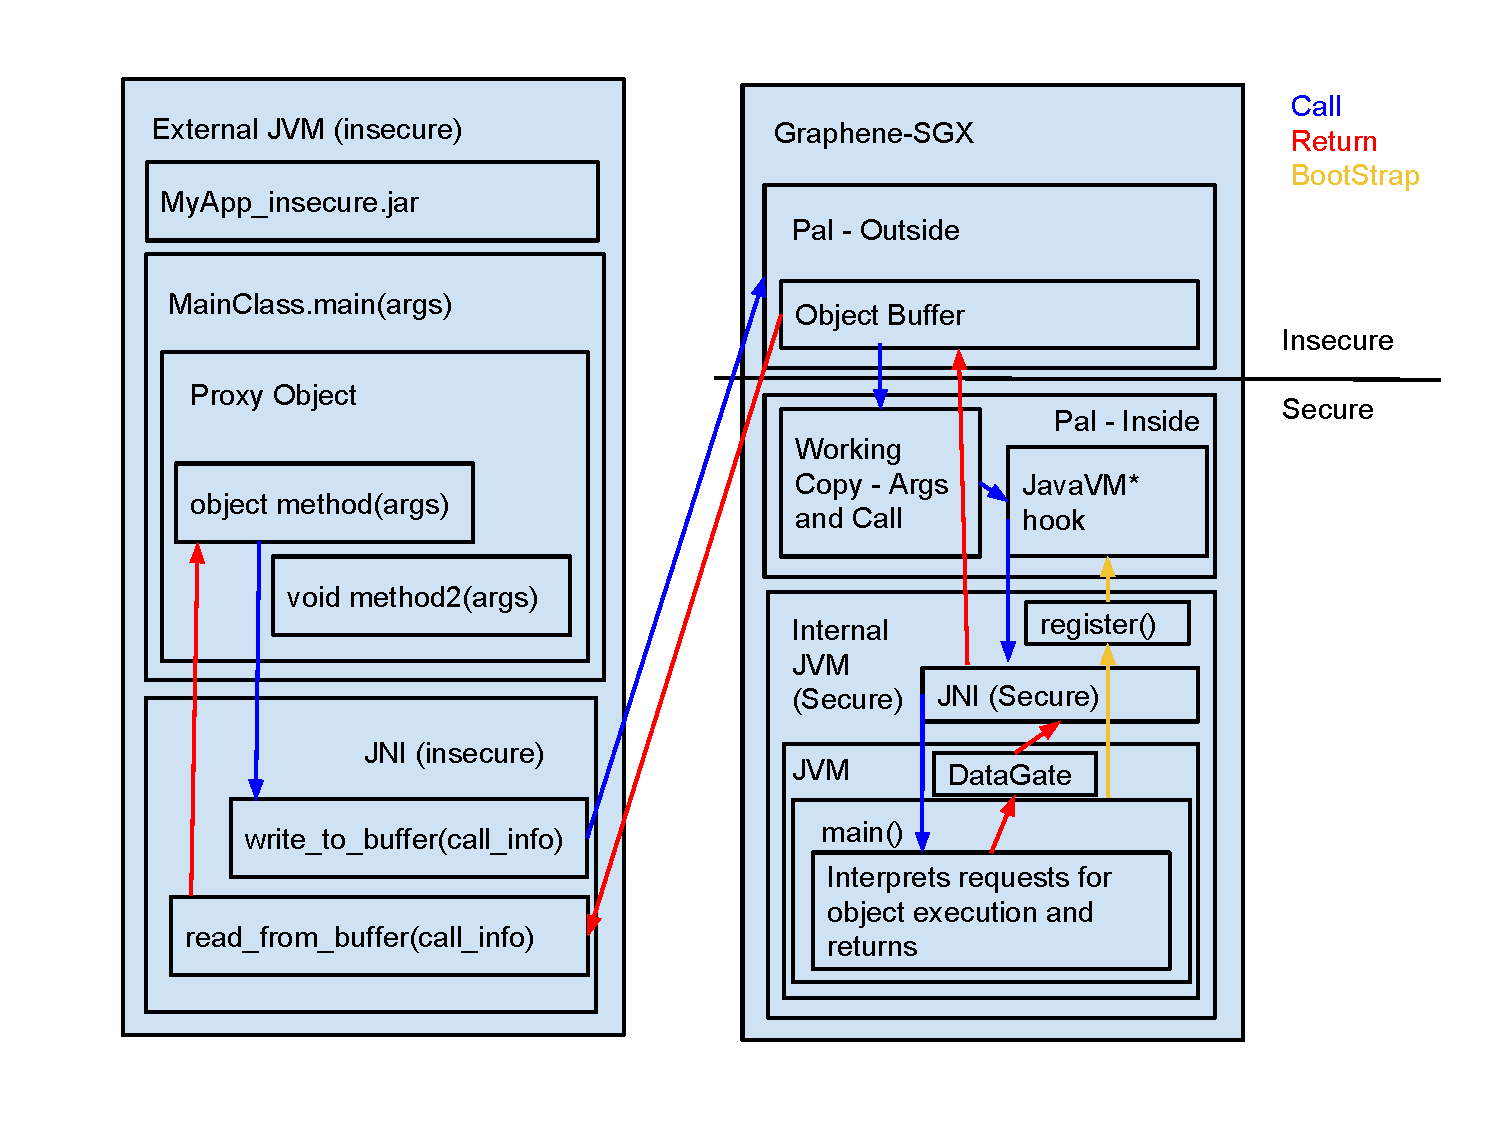
\includegraphics[width=\linewidth]{civet_flow.pdf}}
%\caption{Cevit Architecture and control flow.}
%\label{fig:architecture}
%\end{figure}

%\sysname{} leverages JAVA, a managed language 
%runtime, to help thwart the attacks discussed in 
%section~\ref{sec:background}. The modularity of JAVA 
%allows automatic partitioning of applications to 
%reduce the number of classes added to the Trusted 
%Computing Base. The type-safety property enforced by 
%JAVA runtime avoids exploitation of memory-safety 
%vulnerabilities in the application . JAVA framework 
%also eases the information flow tracking to prevent 
%information leakage due to buggy code. Moreover, 
%\sysname{} uses JAVA runtime to seamlessly 
%provision secure objects and classes in the enclave.




%\subsection{Automatic Partitioning of JAVA Applications}
%\subsection{Preventing Information Leakage}
%\subsection{Seamless Provisioning of Secure Objects and Classes}

\section{Implementation Details}
\label{sec:implementation}

In this section, we discuss in detail about how the framework of \sysname{}
is implemented. 

\paragraph{The \graphene{} \libos{} ported to \sgx{}}
Similar to Drawbridge~\cite{porter11drawbridge}
in Haven~\cite{baumann14haven},
\graphene{}~\cite{tsai14graphene} maps a larger number of Linux system APIs
to a narrow, portable host interface.
Library OSes like Drawbridge and Haven unlock the platform limitations of \sgx{} and
allows many applications to be ported to enclave painlessly.
%The untrusted interface of \graphene{} \libos{} after porting to \sgx{}
%is mostly identical to the original host interface,
%therefore \graphene{} has a finite  bound on interface for the enclave.

%\graphene{} uses checksums to verify the integrity of applications.
%The checksums are collected by a compile-time Signer tool of \graphene{}.
%The Signer tool ensures the integrity of the file checksums
%by including them as part of the enclave's measurement.
%Even if the same \libos{} is used
%to run the applications,
%different binaries in the enclaves yield different measurements. 
%Such a design decouples the problem of distributing 
%and guaranteeing code integrity for each application, as the enclave integrity is based on the integrity of the application --- not just the libOS.
 
\sysname{} makes minor modifications to \graphene{} to allow
the enclave to run
in the same process as the the untrusted \jvm{}.
The trusted and untrusted VM share a ring buffer (as shown in Figure~\ref{fig:runtime} for communication during control transfer,
but the ring buffer itself is not trusted. The \sysname{} framework encrypts tainted security-sensitive data before passing the data on the ring buffer.
 
\paragraph{Control transfer at enclave entry}

\sysname{} transparently transfers the control from the untrusted classes to trusted classes --- triggering enclave entry in the process ---
by intercepting the trusted classes's method or constructor invocation by untrusted classes.
\sysname{} intercepts classes in two ways:
(a) For an entry class that has finite entry points,
\sysname{} creates a wrapper class that redirects all constructors and static methods.
(b) For other trusted classes, \sysname{} adds the redirection calls only when a reference is returned by the enclave. %\fixmebj{Is this correct?}
%(b) For other trusted classes, the interception is installed when a reference of 
%object is returned to the untrusted classes.
On future access of the object in the enclave, a proxy object is created to trigger the interception, using CGLib.

When the control transfers between the trusted and untrusted classes,
the arguments and return values of the methods
are stored in the ring buffer.
\sysname{} relies on serialization and deserialization to safely transfer object in and out of the enclave.
When \sysname{} deserializes an object, the \jvm{} perform type-checking sanitize the input. % the members.

%After \sysname{} transfers the arguments, the \jvm{} thread that
%invoke the intercepted  method does not directly enter the enclave.
%On the other hand, several enclave threads that are pre-created during the enclave creation that are block-waiting on the ring buffer.
%One of the enclave threads consumes the queued job, invokes the method,
%and returns to block-waiting for more new requests.
%No variable on the stack has to be persistent for the enclave threads,
%and only instances of the trusted classes are persisted across enclave entry and exit.

%Moreover, upon enclave entry and exit, the objects that can be safely transferred in or out of the enclave must be serialized / deserialized.
%However, not all classes implement the interface {\tt Serializable},
%especially when the classes contain internal states that cannot be simply interpreted.
%But, \sysname{} assumes that the types of all arguments and return objects must be {\tt Serializable}. 

\paragraph{Limitations}
As we leverage dependency tracking for automated partition, there are few corner cases that the Shredder cannot gracefully handle.
Because CGLib creates subclasses of objects when intercepting them,
it requires the intercepted object to be never finalized.
If a trusted class is also a final class, developers have to manually modify the class definition. Even though final attribute prevents further extension of the class, we argue that the application developer who is building the enclave can safely remove the final attribute as the \sysname{} signs the enclave jar.

 We also do not let trusted classes make method or constructor invocation of the untrusted classes, as the untrusted classes may be able to influence and interfere with the execution of trusted classes. Moreover, we only consider the provisioned code and data as security-sensitive. Even though this limits the usage scenarios, we argue that for any right usage of \sgx{} hardware, these limitations are not disruptive.

%\input{Implementation Details}
%% ASPLOS
%\input{cloud}
%\input{Case Studies}
\section{Case Studies}
\label{sec:case-study}

In order to evaluate the utility of \sysname{}, we partitioned
several example \java{} applications, which we use in our evaluation.


\paragraph{Session Encryption in SSH Client/Server.}
%Code that handles security sensitive data
In order to show the ability of \sysname{} to protect a 
confidential data and avoid leaking that data,
%A \java{} program with a secret that is either generated during runtime
%or provisioned from trusted remote enclaves,
%can be partitioned and secured by \sysname{} to prevent leaking the secret.
%We demonstrate this use case
%using 
we partitioned a \java{}-based SSH client and server~\citep{apache-sshd}.
In this case, the protected secret is the session key.
%For an SSH connection, one primary secret that needs to be secured
%is the session key used for encrypting and decrypting the data
%between the two communicating parties.
For both the SSH client and server, we create
a control class in the enclave that includes 
the key generator, encryption engine objects, secret key
and the {\em BouncyCastle}~\citep{bouncycastle} cryptography library.
The rest of the application is outside of the enclave.
%from the rest of the application.
%\fixmedp{surprising the private key isn't also in the enclave}

We use information flow tracking to ensure that the only data
leaving the enclave is ciphertext output from the encryption algorithm,
or plaintext returned from the decryption algorithm.
This involves adding lines to the end of both algorithms, and does assume that
the encryption and decryption functions are implemented correctly.
Attempts to copy the session key directly into an output buffer at any other point in the code
will result in encryption of the buffer before leaving the enclave.

{\tt org.apache.sshd.common.FactoryManager} is identified as the entry class for Shredder, because this class returns all the objects required for the SSH Protocol.
Shredder generates the enclave image that includes the secret key classes, random generator, key generator, engine for diffie-hellman key-exchange, and encryption-decryption engine. Both the client as well as the server are partitioned to be run using \sysname{}. The client and server first mutually attests each other, exchange the key, and then setup the secure session. We use these SSH client and server for transferring files using SFTP. For simplicity, we run both client and the server on the same host, but in different enclaves. 
%We measure the bandwidth of file transfer as discussed in \S\ref{sec:eval:perf}

%\fixmedp{I took some liberty here: We have to be able to receive data too, right?  Also, I would be more careful with the use of ``guarantee'' in general}

%% The information flow filtering guarantees that no part of the session key
%% can leak from the enclave despite any vulnerabilities 
%% in the crypto library or the control class.
%% The only data that can be released from the enclave
%% is the cipher text of the inputs from the SSH client and server,
%% encrypted with the session key, after declassification.
%% We only had to add only one line of code to declassify the cipher text using the {\tt Enclave.declassify(ciphertext)} API. Thus, in addition to only identifying classes with sensitive information, the developers have to just add one statement per declassifying location in the enclave classes.

\paragraph{Secret Hadoop Algorithm.}
%Code that contains a secret algorithm
\sysname{} not only protects confidential data, but also protects confidential code.
For instance, if a company has developed an analysis tool that gives them a essential competitive advantage,
they must either run their own data center or trust a cloud provider not to leak their tool 
to any competitors.
%, such 
%as trade secret, that developers intend to protect from insecure system stack.

To demonstrate this use case, we modify a Hadoop sort algorithm~\citep{hadoop-sort},
so that the implementation of its Partitioner, Mapper, Combiner, Sorter and Reducer
are isolated from the rest of the Hadoop infrastructure. 
The algorithm sorts values from a key-value store, in which
the input keys and values are encrypted.
The output of the sorting algorithm is a sorted, encrypted key value store.
%based on original values a key-value store, in which
%both input keys and values are encrypted.

The Hadoop framework schedules proxy Partitioners, Mappers, Combiners, Sorters, and Reducers,
and then creates enclaves for these classes.
Once a baseline \sysname{} enclave is created, encrypted class files
are downloaded from a trusted server using our remote attestation tools,
and then decrypted, loaded, and measured for integrity. 
%We evaluate the Job completion time for our sort algorithm in \S\ref{sec:eval:perf}.
%, requests for the real classes to be provisioned from a trusted server, loads, and executes the provisioned classes.

The information flow control at the enclave border protects against
accidental output of a plaintext key-value pair from the encrypted store,
as well as protects the class code file itself.
Similarly, intermediate state from the code cannot be inadvertently returned by a function to the untrusted Hadoop framework,
although we do allow encrypted outputs to be passed from a Mapper to a Combiner or Reducer.
The contents of any code cannot be leaked outside enclave by copying the code into an output object, as the tainted object is automatically encrypted before leaving enclave. %\fixmedp{does this just happen naturally?},
Also, in conjunction with the trusted remote server, we rate-limit instantiations of the code to mitigate the risk of
brute-force mapping of its outputs or reverse-engineering the code.


%% any output of the isolated classes ---
%% even if it is just an intermediate state ---
%% is encrypted before leaving the enclave.
%% \sysname{} not only protects the implementation of the algorithm,
%% but any output of the algorithm that may potentially help attackers
%% reverse-engineer the implementation. The {\em confidential code} property of ~\sysname{} is not limited to Hadoop, but can also be leveraged by standard \java{} applications.

\paragraph{Secure Data Manager Web-app.}
%JAVA Web-start Application
\sysname{} can also secure {\em Java Network Launch Protocol} (JNLP) applets and web-start apps, effectively 
extending trust from a remote trusted server to a client enclave using any web-app 
plugged into a supported browser. This allows the developers to offload some of the 
computation on secret data to the client machine from the trusted server.
%\java{} applications in the form of
%can also be secured by \sysname{}. 

For instance, in a large medical hospital with a centralized repository of patient data,
the doctors may want to access any patient data from any terminal using a web browser.
A web developer can design an applet such as Secure Data 
Manager(SDM)~\citep{sdm-applet} to store the secret patient data on a client machine, 
and display this information securely using Intel Protected Audio and Video Path 
(PAVP) technology~\citep{intel-pavp}.
However, to protect the sensitive patient information from untrusted system stack, the 
developer can use \sysname{} to isolate the classes that represent the secure data 
in an enclave. The developer just has to identify such classes representing the secret 
data and display methods, and the \sysname{} seamlessly creates enclave for 
managing secret data.
% or perform computations on secret data isolated in an enclave.
%We demonstrate this use case using a 
%\fixmedp{what is the practial use case?  Like, what is the data actually used for?}
The trusted data manager class authenticates the doctor and loads the provisioned data 
from the remote trusted server. The Intel PAVP enabled displays can then take the input from the display methods of the trusted data manager class.

For simplicity, we only partition and run the SDM applet from a browser without the support for Intel PAVP display devices. We identify four classes --- {\tt SafetyBox}, 
{\tt AuthenticationInfo}, {\tt LoginEntry}, and {\tt Type} --- as entry class to the Shredder and generate a web-start app image containing the enclave image. The web-app loads normally, and when it tries to access any of the above four classes, \sysname{} seamlessly creates an enclave for those objects. 
%We measure the latency of I/O from the SDM in \S\ref{sec:eval:perf}.


%\fixmedp{This last example is pretty content free.  Can you give me an example of a web app that would use this, and flesh out the story a bit?}

\chapter{Evaluation}
\label{chap:eval}
%\subsection{Other Related Works}

\section{Summary}
\label{sec:graphene:summary}

The \graphene{} design is centered around
building a para-virtualized layer, which can reuse the OS components for reproducing Linux system interfaces.
%instead of building arbitrary compatibility layers for reproducing the system interface.
%constantly porting the significant  of the existing system interface.
%In \graphene{}, 
\graphene{} defines a host ABI, as a new boundary between the OS and user space.
The host ABI is simple enough to port (containing \palcalls{} functions),
and exports sufficient functionality for virtualizing a primary part of the system API components.
A library OS is built upon the host ABI,
and implements \graphenesyscalls{} Linux system calls to reuse unmodified Linux applications.
\graphene{} decouples the development for a compatibility layer,
from host-specific challenges to building OS features, and isolating applications from other malicious tenants.



%\sysname{} extends library OS designs 
%to include multi-process APIs required by common applications, such as a shell or 
%web server.
%\sysname{} demonstrates efficient, selective
%coordination of shared state across multiple library OS 
%instances---maintaining host independence.
%%simplifying security sandboxing of otherwise unwieldy OS features.
%Applications on \sysname{} enjoy both 
%strong security isolation with acceptable performance and low memory overheads.
%% from unrelated programs 
%%and seamless shared namespaces 
%%among a group of coordinating guests.
%%% Although this paper focuses on distributed coordination
%%% to facilitate the efficiency benefits,
%%% expect our experiences with distributed coordination 
%%% may also be particularly relevant to highly scalable OS designs, 
%%% which avoid the bottlenecks of shared OS data structures~\cite{baumann09barrelfish, song11eurosys}.
%%Graphene's overheads are acceptable and the memory 
%%footprint is substantially lower than a VM.



%% , which could benefit from the reduced memory footprint
%% in a cloud 

%% by introducing a novel design for  coordination APIs. 
%% to a new OS (Linux),
%% new classes of applications,
%% and introduces a
%% %an alternative design point for storage virtualization.
%% Our results further demonstrate the feasibility of the library OS model.
%% % generally,
%% Applications on Graphene enjoy both 
%% strong security isolation from unrelated programs 
%% and seamless shared namespaces 
%% among a group of coordinating guests.
%% Although we explore this concept in a library OS,
%% we expect the namespace coordination framework 
%% could also be adapted to limit the attack surface area between
%% processes in a traditional OS.
%% We expect these experiences with distributed coordination 
%% may also be particularly relevant to highly scalable OS designs, 
%% which avoid the bottlenecks of shared OS data structures~\cite{baumann09barrelfish}.
%and specifically of content-addressable storage as the primary virtual storage abstraction.
%%% This work opens up a number of interesting questions for future work, 
%%% including studying opportunities for low-level storage optimization within the CAS server,
%%% making CAS the root file system,
%%% eliminating storage management in the host kernel, and 
%%% investigating the impact of frequent migration among devices.

\begin{comment}
Enabling legacy applications in a restricted environment,
such as \picoprocs{} or enclaves,
requires extra effort for mitigating the limitations of platforms,
in order to support typical OS personalities.
\graphene{}, as described in this chapter, extends the existing \libos{} designs
from isolating single-process or unshared abstractions
to include multi-process APIs required by many UNIX applications,
such as servers or shell scripts.
The challenge that \graphene{} primarily overcomes
is the requirement for coordinating shared states across multiple \picoprocs{},
to provides a collaborative, unified OS view.
Essentially, \graphene{} implements all shared, multi-process abstractions
and OS states
based on coordination over host-provided, pipe-like RPC streams.
The RPC-based, distributed OS implementation enables multi-process support in \graphene{}, with minimal extension to the host interface,
and a sweet-spot for enforcing inter-application security isolation,
by simply sandboxing the RPC streams.
Such a model largely reduces the complexity of
enforcing security isolation
on idiosyncratic multi-process abstractions
and shared states.
Because the corporative nature of \picoprocs{} in \graphene{},
an application can even dynamically impose sandboxing on one of its processes,
to reflect per-process, variable security policies.
\end{comment}

\begin{comment}
In principle, we attempt to use \graphene{} to justify the platform independence
of the \libos{} design,
without sacrificing its qualitative benefits,
such as isolating mutually-untrusting applications
and a narrow attack surface to kernels.
\graphene{} implements a considerable number of common Linux system calls,
to support popular, modern applications
such as Apache web server, GNU Make, OpenJDK \java{} VM and the Python runtime.
\graphene{} translates the high-level system APIs used by applications
to a host ABI
inherited and extended from a previous Windows-compatible \libos{}~\cite{porter11drawbridge}.
In addition, we port the \pal{} (Platform Adaption Layer) of \graphene{}
to various platforms,
including FreeBSD, OSX, Windows, and even a more restricted environment, the \intel{} \sgx{} enclaves.
In particular, \graphene{} being ported to \intel{} \sgx{}
(\graphenesgx{})
can isolate applications --- either single-process or multi-process
--- on a host where neither the operating system nor the hardware (except the CPU package)
is trusted by the applications. 
Overall, \graphene{} shows that,
by simply porting the reasonably sized host ABI
to a new platform,
a whole large spectrum of legacy applications tested on the previous platforms
can be activated all together.
\end{comment}


\makeatletter
\def\input@path{{}}
\makeatother
\graphicspath{{}}

\declarecommand{\dentry}{dentry}
\declarecommand{\dentries}{dentries}
\declarecommand{\Dentry}{Dentry}
\declarecommand{\Dentries}{Dentries}
\declarecommand{\vnode}{{\tt vnode}}
\declarecommand{\vnodes}{{\tt vnodes}}
\declarecommand{\dcache}{{dcache}}
\declarecommand{\inode}{{inode}}
\declarecommand{\dnlc}{{\tt DNLC}}
\declarecommand{\fnone}{{X}}
\declarecommand{\fntwo}{{Y}}
\declarecommand{\fnthree}{{Z}}
\declarecommand{\fnfour}{{A}}
\declarecommand{\fnfive}{{B}}
\declarecommand{\fnsix}{{C}}
\declarecommand{\lnone}{{L}}
\declarecommand{\lntwo}{{R}}
\declarecommand{\completeflag}{{\tt DIR\_COMPLETE}}
\declarecommand{\lookupflag}{{\tt NEED\_LOOKUP}}

\declarecommand{\ubuntuver}{{14.04}}
\declarecommand{\linuxver}{{3.14}}
\declarecommand{\prefixcheckcachesize}{{4}}
\declarecommand{\PCCsize}{{64 KB}}
\declarecommand{\lookuptablesize}{{64}}
\declarecommand{\lookuptableway}{{2}}

\declarecommand{\statspeedup}{{26}}
\declarecommand{\openspeedup}{{13}}
\declarecommand{\slowpathcost}{{xx}}
\declarecommand{\dentryoldsize}{{192}}
\declarecommand{\dentrynewsize}{{192}}
\declarecommand{\dentrysizeoverhead}{{64}}
\declarecommand{\dovecotspeedup}{{12}}
\declarecommand{\gitspeedup}{{7}}
\declarecommand{\updatedbspeedup}{{29}}

\newcolumntype{L}[1]{>{\raggedright\let\newline\\\arraybackslash\hspace{0pt}}m{#1}}
\newcolumntype{C}[1]{>{\centering\let\newline\\\arraybackslash\hspace{0pt}}m{#1}}
\newcolumntype{R}[1]{>{\raggedleft\let\newline\\\arraybackslash\hspace{0pt}}m{#1}}

\chapter{Related Work: Dcache Optimization}

%\section{Introduction}
%\label{sec:dcache:introduction}

Operating System kernels commonly cache file system data and metadata in 
a virtual file system (VFS) layer, which abstracts low-level file systems into a common API, 
such as POSIX.  
This caching layer has become a ubiquitous optimization
to hide access latency for 
persistent storage technologies, such as a local disk.
%whether a local disk or a network appliance, 
%have substantially higher access latencies than RAM,
%this caching layer 
%% SOSP Space - kind of quacking on
%% Caching
%% the file system directory hierarchy is particularly important because 
%% low-level file systems often spread this information across 
%% multiple disk sectors.
%% If an application wanted to open a single file on a system without a directory cache, 
%% most low-level file systems would issue numerous disk reads to locate the file and check the permissions
%% on the file and its parent directories;
%% a directory cache can commonly avoid these reads.
The directory cache is not exclusively a performance optimization; it also simplifies 
the implementation of {\tt mount}-ing multiple file systems, 
consistent file handle behavior,
and advanced security 
models, such as SELinux~\citep{selinux}.



%\fixmedp{Be charitable to developers, make our strong claims positively (we are really smarties) rather than calling them dummies}


%% Many observation shows that, in most systems, operations to storage are often
%% dominated by hierarchical structure traversal,
%% and fetching metadata of objects.\fixmetsai{references here}~\citep{duchamp94nfs}
%% In many file systems, traversal and metadata fetching
%% create random access patterns,
%% which are slower than sequential access patterns
%% on many storage media, e.g. magnetic disks.

% dp: I think this is getting down in the weeds.  We need to make the case for the work 
%     more strongly and generally first
%% Directory entry cache, a.k.a \dcache{},
%% is an important optimization in Linux kernels
%% to reduce storage operations for traversal and metadata fetching.
%% The design of \dcache{} is comparable to \vnode{} in BSD and \dnlc{} in Solaris.
%% \dcache{}, as well as \vnode{} and \dnlc{},
%% can be explained as a file system layer that
%% responds to requests on a cache hit,
%% but passes requests down to lower-leveled file systems on a cache miss~\citep{zadok06, skinner93}.

%\fixmedp{F1: Maybe thread together an argument about why no one would have tried a one-hop lookup before?}


%\marginpar{\scriptsize \textcolor{blue}{ Michael, I think the high-order bits are mostly right on Fig~\ref{fig:dcache:lookup-frac},
%but these number may change a bit as we refine the measurement}}

\begin{figure}[t]
\scriptsize
\centering
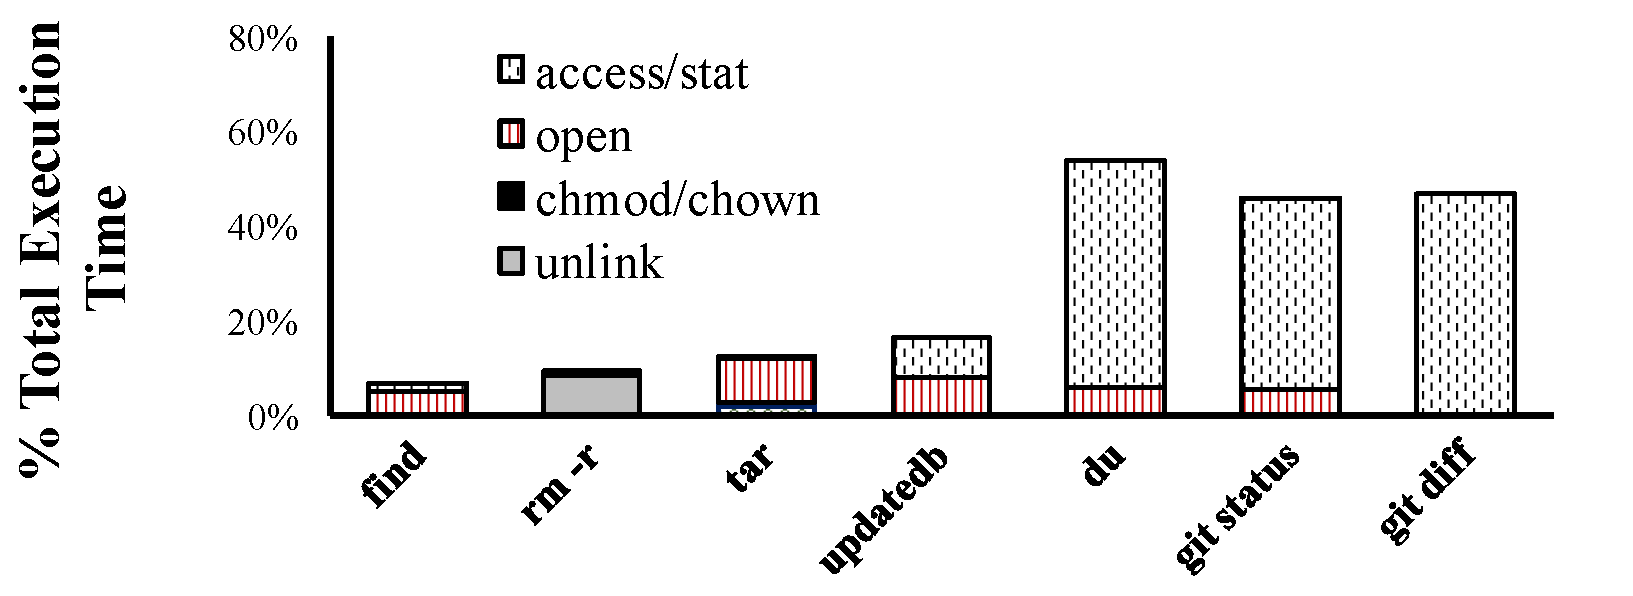
\includegraphics[width=5in]{dcache/plots/syscall-percentage.pdf} \\
\caption[Fraction of execution time on path-based system calls.]
{Fraction of execution time in several common utilities spent
executing path-based system calls with a warm cache, as measured with ftrace.}
\label{fig:dcache:lookup-frac}
%\vspace{-10pt}
\end{figure}

%\fixmedp{Please check these \% against time.  I think git diff is too high.  git status seems ok.}

Directory caches are essential for good application performance.
%Unix was designed such that ``(almost) everything is a file'',
%thus even accesses to in-memory file systems, device files, FIFOs and domain sockets
%first pass through the directory cache.
%In other words, 
Many common system calls must operate on file paths,
which require a directory cache lookup.
For instance, between 10--20\% of all system calls in the iBench system call traces do a path lookup~\citep{filenotafile}. 
Figure~\ref{fig:dcache:lookup-frac} lists the fraction of total execution time
%, as well as system time, 
several common command-line applications spend executing path-based system calls
(more details on these applications and the test machine in \S\ref{sec:dcache:eval}).
We note that these system calls include work other than path lookup,
and that these numbers include some instrumentation overhead;
% are coarse measurements that include  and work than path lookup;
%, and includes some time 
%for synchronous I/O (e.g., during {\tt rename}) as well as non-path tasks (e.g., creating 
%a file handle as part of {\tt open});
nonetheless, in all cases except {\tt rm},
the system call times and counts are dominated by
{\tt stat} and {\tt open}, for which 
%can be serviced from cache and for which 
path lookup is a significant component of execution time.
For these applications, path-based system calls account for 6--54\% of total execution time.
%and 25--77\% of system time.  
This implies that
lowering path lookup latency is
 one of the  biggest 
opportunities for a kernel to improve these applications' execution time.




\begin{figure}[t!]
\centering
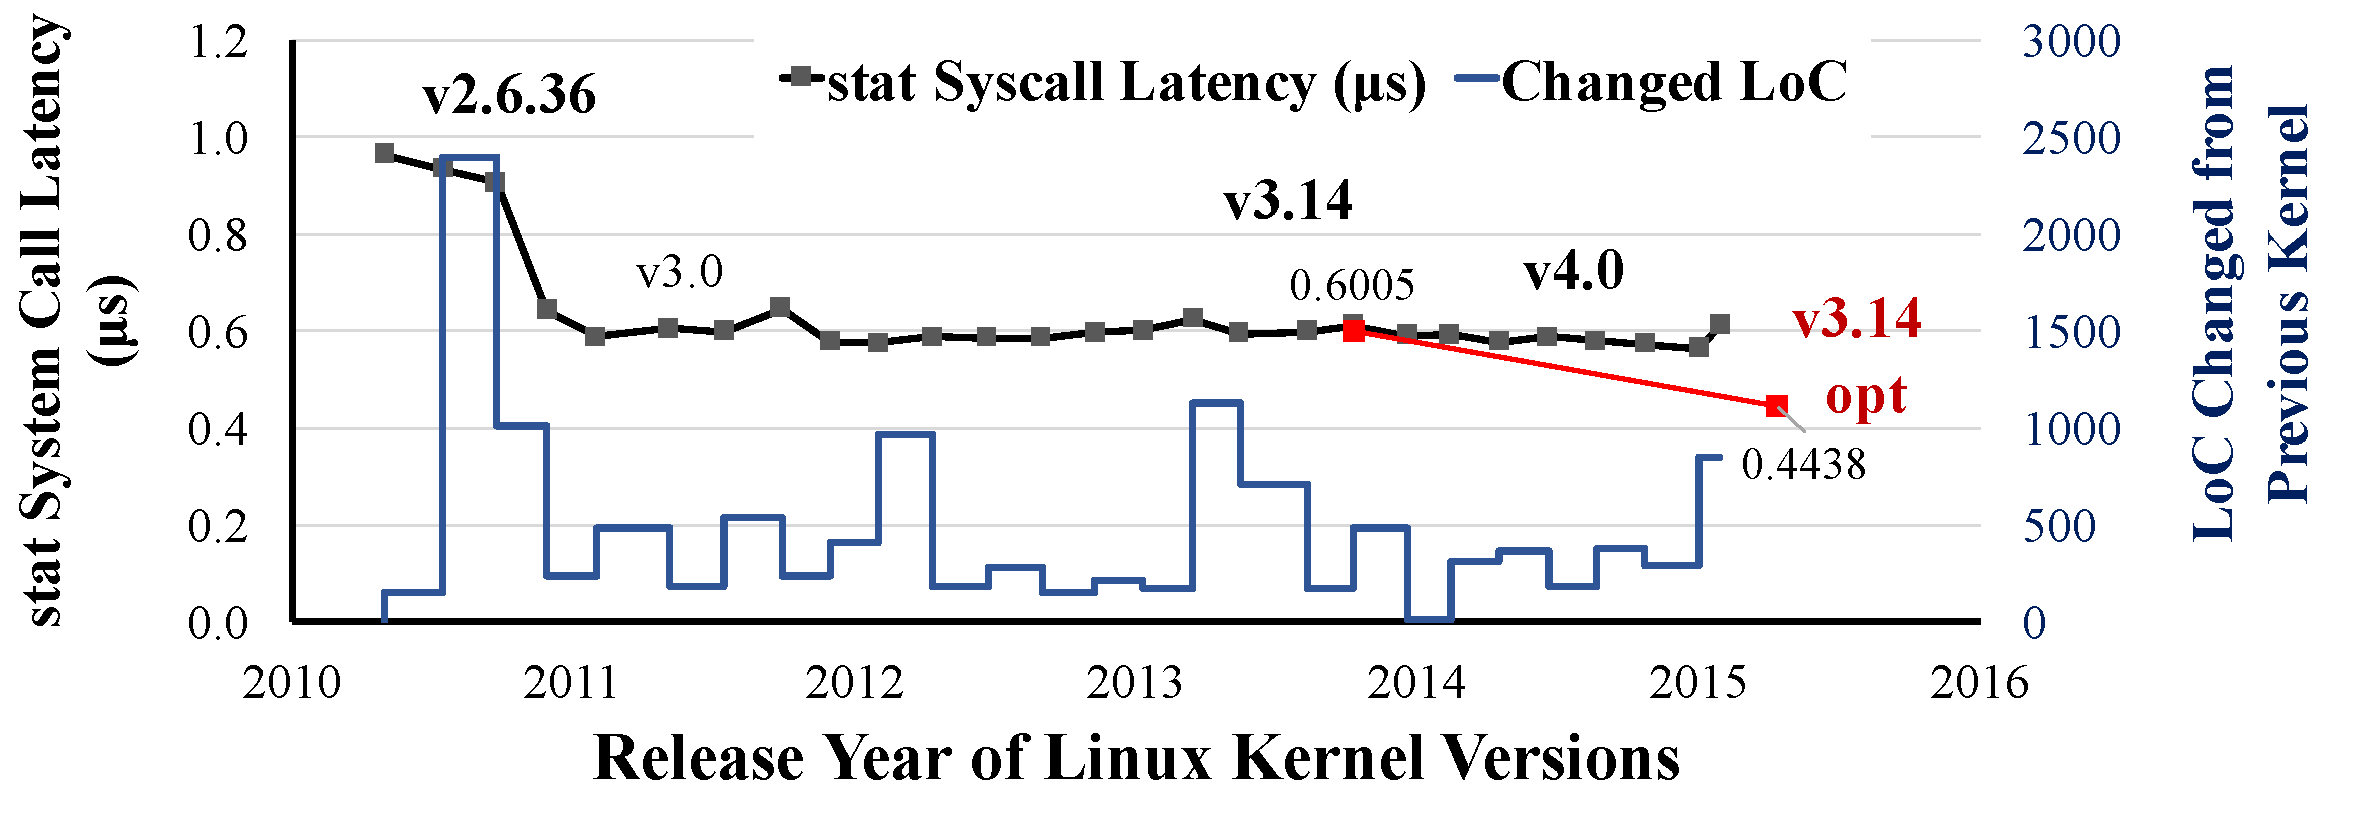
\includegraphics[width=6in]{dcache/plots/latency-by-version.pdf}
\footnotesize
\caption[Lantecy of {\tt stat} system call over years.]
{Latency of {\tt stat} system call with a long path {\tt XXX/YYY/ZZZ/AAA/BBB/CCC/DDD/FFF} on Linux over four years (lower is better), as well as the churn within the directory cache code (all insertions in {\tt dcache.c}, {\tt dcache.h}, {\tt namei.c}, {\tt namei.h} and {\tt namespace.c}). 
%Our optimizations significantly improve performance that has otherwise plateaued, despite significant ongoing developer effort.  
Our optimized \linuxver{} kernel 
further reduces {\tt stat} system call latency by \statspeedup{}\%.}
%\vspace{-15pt}
\label{fig:dcache:by-version}
\end{figure}


%\fixmedp{Add more evidence of lookup importance here: For instance, fraction of lookup time in file-related syscalls, or total lookup time in applications bound on file lookup latency.  }
Unfortunately, even directory cache hits are costly---0.3--1.1 \us{} for a {\tt stat} on our test Linux system, compared to only .04 $\mu$s for a {\tt getppid} and 0.3 \us{} for a 4 KB {\tt pread}. 
%\fixmetsai{Don, check this, I think read will be a better example, getppid is too trivial.}
This issue is taken particularly seriously in the Linux kernel community, which has 
made substantial revisions and increasingly elaborate optimizations to reduce the hit cost
of its directory cache, such as removing locks from the read path or replacing lock ordering with deadlock avoidance in a retry loop~\citep{corbet09jls,dcache-rcu}.
Figure~\ref{fig:dcache:by-version} plots directory cache hit latency against  lines of directory cache code changed 
over several versions of Linux, using a path-to-inode lookup \microbench{} on the test system described
in \S~\ref{sec:dcache:eval}.
These efforts have improved hit latency by 47\% from 2011 to 2013, but have plateaued
for the last three years.
%\fixmedp{if time, filter irrelevant changes from code deltas}
%at the cost of substantial developer effort.
%This latency appears to have plateaued 

The root of the problem is that the POSIX path permission semantics
seemingly require work that is linear in the number of path components,
and severely limit the kernel developer's implementation options.
%The root of this problem is that current directory cache
%designs reflect a straightforward implementation of the POSIX specification,
%which would seemingly require work that is linear in the number of path components.
For instance, in order to open file {\tt /\fnone{}/\fntwo{}/\fnthree{}} 
%for reading, 
one must have search permission
to parent directories {\tt /}, {\tt /\fnone{}}, and {\tt /\fnone{}/\fntwo{}},
as well as permission to access file {\tt \fnthree{}}.
The Linux implementation %of this specification is straightforward, 
simply walks the directory
tree top-down to check permissions.  
Unfortunately, when the critical path is dominated by 
walking a pointer-based data structure, 
including memory barriers on some architectures for multi-core consistency, 
modern CPUs end up stalling on hard-to-prefetch loads.
Moreover, because so many Linux features are built around this behavior, such as Linux Security Modules (LSMs)~\citep{wright+lsm},
namespaces, and mount aliases, it is not clear that any data-structural enhancements
are possible without breaking backward-compatibility with other Linux kernel features.
A priori, it is not obvious that a faster lookup algorithm, such as a single hash table lookup, 
can meet these API specifications and kernel-internal requirements; to our knowledge,
no one has tried previously.

%This paper proposes a decomposition of the directory cache, which allows
%most lookup operations to execute with a single hash table lookup (\S\ref{sec:dcache:dcache}),
%as well as optimizations to reduce the miss rate based on information that is {\em already in the cache}, but not used effectively (\S\ref{sec:dcache:readdir}).
%Our design maintains compatibility (\S\ref{sec:dcache:generalize}) through 
%several essential insights, including 
%how to separate the indexing of paths from checking parent permissions,
%and how to effectively and safely memoize the results of access control checks.


%% This paper proposes several new ways to organize a directory cache, which can yield 
%% substantial performance improvements over the current state of the art.
%% %This paper demonstrates that, despite this developer effort, there is still a substantial 
%% %missed opportunity hiding behind historical, intuitive, but not fundamental design choices.
%% Most of the Linux directory cache design reflects a straightforward implementation of the POSIX 
%% specification. %, with a division of labor that is suitable for mainstream file systems.

%This paper presents an alternative directory cache organization, which 
%improves performance by separating logical tasks, such as separating path indexing from permission checking; yet the design is sufficient to retain compatibility with POSIX.
%In the case of path lookup, 
%this paper demonstrates how 
%a per-component tree walk can be replaced with a single hash table lookup (\S\ref{sec:dcache:dcache}).
% without violating POSIX compliance.

%Our optimizations improve the performance of frequent lookup operations, but 
%introduce several costs, described in \S\ref{sec:dcache:dcache} and measured in \S\ref{sec:dcache:eval},
%which  we believe are acceptable and a net improvement for applications.
%First, these optimizations slow down infrequent modifications to the directory hierarchy, such as {\tt rename}, {\tt chmod},
% and {\tt chown} of a directory. 
%However, these slower operations
%account for less than .01\% of the system calls in the iBench traces~\citep{filenotafile}.
%Second,  the memory overheads of the dcache are increased.
%%(45\% per \dentry{}, as well as some  in our prototype).
%%(\fixmedp{XX MB} in our tests).  
%Third, lookup has a 
%probability of error from signature collisions that can be adjusted to be negligible
%%($2^{-141}$ in our configuration), 
%and within acceptable thresholds widely used by data deduplication systems~\citep{Debnath:2010:CSU:1855840.1855856, Srinivasan:2012:ILI:2208461.2208485, Quinlan:2002:VNA:645371.651321, Zhu:2008:ADB:1364813.1364831}.
%%, as well as how to remove
%%all memory barriers from the lookup path (\S\ref{sec:dcache:update}).
%In the micro-benchmark of Figure~\ref{fig:dcache:by-version}, our directory cache 
%optimizations improve lookup latency by 
%%revisions improve latency of accessing a long path
%%by 
%\statspeedup{}\% over unmodified Linux.
%%Our design addresses other missed
%%opportunities, such as identifying new opportunities to reduce the miss rate
%%through caching directory completeness.
%%\fixmedp{Do we want to highlight LoC?  3K is more than anything in the graph} \fixmetsai{Probably just mention in the evaluation. It's a metric that we should provide, but it's not awfully interesting.}
%%The total lines of code changed are fewer than 3,000 out of \fixmedp{XX}.
%%\fixmedp{Can we get 
%%, yet changes fewer than 3,000 lines of code.

%% SOSP cut - kind of long-winded
\begin{comment}
This paper rethinks current Linux directory cache design choices in light of the following goals:
\begin{compactitem}
\item {\bf Minimize the cost of a cache hit.} (\S\ref{sec:dcache:dcache}).
This means maximizing the benefit of temporal locality for frequent operations,
while pushing extra work of consistency maintenance onto less frequent, already-expensive operations.
%such as handling cache miss or updating massive metadata,
%in order to improve very frequent operations.
\item {\bf Maintain legacy compatibility.} (\S\ref{sec:dcache:generalize}).  Unix path semantics are complex, required by applications, file systems, and security modules, frustrating otherwise straightforward optimizations.  However tempting it may be to redesign path behavior to facilitate caching, path operations must exhibit the same behavior, with lower latency.
\item {\bf Never miss the same request twice in quick succession.} (\S\ref{sec:dcache:readdir}).  A number of less-frequent operations, such as reading a directory or secure temporary file creation, always miss in the cache {\em even if enough information is in cache to satisfy the operation.}  
%Of course, infrequent accesses should still be subject to a cache replacement policy, such as LRU.
\end{compactitem}
%Although directory caches must implement more complex semantics than a hardware memory cache,
%these principles should seem familiar to the reader with a basic architecture background.
%sadly, the Linux directory cache design violates all three.
\end{comment}

%This paper introduces several techniques to improve the performance of a directory cache,
%This paper explains several practical directory cache optimizations,
This paper demonstrates that these techniques improve performance for applications that use the directory cache heavily,
and the harm is minimal to applications that do not benefit.
%and that the worst case \microbench{} is only 12\% slower within \fixmedp{XX}\% of unmodified Linux.
%Each optimization we describe improves performance in isolation, and all can be combined.
%These optimizations change very few lines of code, and are backward-compatible with 
%legacy applications.  
%These changes are encapsulated in the VFS---individual file systems do not have to change their code.
%This paper describes a  prototype of these improvements implemented in Linux \linuxver{}.
%\S~\ref{sec:dcache:background} explains that the directory cache structure of Mac OS X, FreeBSD, and Solaris 
%are sufficiently similar that these principles should generalize.
%we compare and contrast Linux's directory cache
%with Mac OS X, FreeBSD, and Solaris in \S\ref{sec:dcache:background}, and explain inline how each
%optimization could be generalized to these other OS kernels.





%% \item {\bf Modularization and stackability}:
%% Any changes or optimizations must be implemented as modules inside Linux's VFS,
%% and can be stacked on top of the original design or any future optimizations. 
%% \item {\bf Backward compatibility}:
%% Any changes or optimizations must maintain least requirement of modifying any
%% file systems.
%% \item {\bf Generalization to other OSes}: Any changes or optimizations must be portable to other OSes with reasonable effort and change of design.




%% \dcache{} is proven to be effective on improving storage performance.
%% Experiments shows that,
%% in a Linux 3.x kernel, a \dcache{} with a xxx\% hit rate can speed up
%% metadata lookup and fetching time by xxx times.
%% \fixmetsai{experiment result, Linux version, and fs specs here}
%% However, we observed that Linux maintainers have made
%% constant and non-trivial efforts to improve \dcache{} in the Linux kernel.
%% We studied all \dcache{}-related source files in the Linux kernel Git repository,
%% and discovered that maintainers have committed
%% on average xxx revisions per source files.

%% We tested metadata lookup time on primary \dcache{}-related revisions.
%% Most changes on \dcache{} system only create xxx\%-xxx\% speed-up
%% than their predecessor.
%% \fixmetsai{result and graph here}.
%% Moreover, improvement to \dcache{} is still work-in-progress
%% for Linux maintainers.
%% \fixmetsai{reference to threads for latest dcache discussions}. 
%% All the evidences show that,
%% despite of significant reduction of storage operations,
%% efficiency of \dcache{} system internally still remains as a concern.

%% We argue that the design of \dcache{} needs to be carefully re-examined,
%% to fundamentally identify any missed opportunities that
%% improve value of \dcache{}.
%% At a high level, most optimization works for \dcache{} are focused on
%% improving ``how to cache'',
%% but we want to also lay eyes on ``what to cache'',
%% to ensure any valuable information returned from file systems
%% be captured by \dcache{} system.

%The contributions of this paper are as follows:
%\begin{compactitem}
%\item A performance analysis of the costs of path lookup and the opportunities
%to improve cache hit latency.
%\item A directory cache design that improves path lookup latency with a combination of techniques, including:
%  \begin{compactitem}
%  \item Indexing the directory cache by full path, reducing average-case lookup from linear to constant in the number of path components.
%  \item A Prefix Check Cache (PCC) that separates permission checking from path caching.  The PCC memoizes permission checks, and is compatible with LSMs~\citep{wright+lsm}.
%  \item Reducing the cost of checking for hash bucket collisions with path signatures.
%  \end{compactitem}
%\item Identifying opportunities to leverage metadata the kernel already has to reduce miss rates, such as tracking whether a directory is completely in cache.
%\item Carefully addressing numerous, subtle edge cases that would frustrate rote application of these techniques, such as integration with symbolic links and Linux namespaces.
%\item A thorough evaluation of these optimizations.  For instance, our optimizations improve throughput
%of the Dovecot IMAP server by up to \dovecotspeedup\% and latency of 
%updatedb by up to \updatedbspeedup{}\%.
%%git version control system by up to 25\%.
%
%\end{compactitem}

\section{Background}
\label{sec:background}

This section summarizes \sgx{},
and current design points for running or porting applications on \sgx{}.
%and the legacy frameworks of porting 
%including \haven{}~\cite{baumann14haven}, \scone{}~\cite{osdi16scone}, and Panoply~\cite{shinde17panoply}. 


\subsection{Software Guard Extensions (SGX)}
\label{sec:background:sgx}

%\begin{figure}[t!]
%\centering
%\includegraphics[width=\linewidth]{figures/libosvssdk.pdf}
%\footnotesize
%\vspace{-0.3in}
%\caption{
%Comparison between libOS-based model (e.g., \haven{} and \graphenesgx{})
%and SDK-based (SDK for \sgx{}) model for migrating applications in enclaves.
%Green (light) boxes are trusted components and red (dark) boxes are untrusted.
%The libOS-based model often yields a larger TCB in the enclave,
%while the SDK-based model requires developers to be responsible of
%securing the enclave on the untrusted interface.
%}
%\label{fig:libosvssdk}
%\end{figure}

The primary SGX abstraction is an \emph{enclave}: an isolated execution environment within the virtual address space of a process.
The code and data in enclave memory do not leave the CPU
package unencrypted; when memory contents are read back into cache,
the CPU decrypts the contents, and checks the integrity of cache lines and the virtual-to-physical mapping.
SGX also cryptographically measures the integrity of enclaves at start-up, and 
provide attestation to remote systems or other enclaves.
%Remote entities can identify the owners of enclaves by distinguishing the cryptographic measurements
%generated with different signing keys.

%%% \sgx{} is a new feature on the 6th-genaration \intel{} CPUs.
%%% it contains a set of new x86/64 instructions, to initiate, destroy, and attest isolated execution environments (i.e., enclaves) in the address space of applications.
%%% When \sgx{} loads an application in an enclave,
%%% the code and data of the application will remain encrypted in the main memory,
%%% forbidding any mean to eavesdrop the application secrets.
%is a set of new x86/x64 instructions introduced
%to the latest \intel{} CPUs,
%to bootstrap an isolated execution environment
%inside applications' virtual memory address space.
%\sgx{} creates a memory region
%(generally referred as {\bf enclave}), storing both the code and data of the isolated execution,
%which stays encrypted in DRAMs and only the CPU is capable of encryption and decryption.
%The CPU derives the encryption key
%from the cryptographic measurement of the initial state of enclave memory,
%to allow remote entities to verify the soundness of execution and establish the trust
%needed for provisioning sensitive data.

\sgx{} enables a threat model where one only trusts the \intel{} CPUs and the 
code running in the enclave(s).
%whereas the rest of application, system software, off-CPU-package hardware devices and providers are untrusted. 
\sgx{} protects applications from three different types of attacks on the same host, which are summarized in Figure~\ref{fig:sgx-threats}: untrusted application code inside the same process but outside the enclave; operating systems, hypervisors, and other system software;
%\fixme{added Mona's suggestion}
other applications on the same host; and off-chip hardware.
A SGX enclave can also trust a remote service or enclave, and be trusted after inter-platform attestation~\cite{sgx-attestation}.




%%% \begin{compactenum}

%%% \item {\bf Inside process memory:}
%%% \sgx{} partitions the application process into two privilege levels, as the trusted part (in enclaves) which can access the whole process memory, and the untrusted part (outside enclaves) forbidden to access enclave memory.
%%% %the privileged part (in the  enclave region) can access all process memory,
%%% %while the unprivileged part (outside the enclave region) is limited to access only data that are not isolated by \sgx{}.

%%% \item {\bf From hosting OSes or hypervisors:}
%%% \sgx{} assumes that OSes and hypervisors can be compromised by either exploiting system vulnerabilities
%%% or malicious system software installed by administrators.
%%% Both types of compromise are legitimate threats to modern OSes, due to complexity of modern OSes and usage of public facilities like clouds.

%%% %Operating systems or hypervisors
%%% %that are either compromised by rootkits
%%% %or deliberately modified by the host providers.
%%% %An attacking host can access the raw data in DRAMs, or remap the
%%% %physical pages to other contexts.

%%% \item {\bf Physically from the hardware:}
%%% One type of attacks that cannot be defended by software-based solutions~\cite{flicker, criswell2014virtualghost}
%%% is from the attackers who have physical access to the hosts.
%%% \sgx{} can resist attacks on the host hardware
%%% including hacking peripheral devices like ethernet cards and connectors~\cite{hudson15thunderstrike}, tapping into buses, or eavesdroping DRAM data using Cold-boot attack~\cite{halderman09coldboot}.


%%% \end{compactenum}


%%% \sgx{} protects an application against unpredictable threats from both local and remote hosts.
%%% \sgx{} establishes a trusted path
%%% from one enclave to another,
%%% providing end-to-end protection to both enclaves to
%%% exchange data with confidentiality and integrity.
%%% %, processing the data and returning the computation results with end-to-end protection.
%%% We can further divide up the protection using \sgx{} into three elements:
%The use cases of \sgx{} mostly involve the process that an enclave
%retrieves a signed attestation from the processor,
%to exchange provisioning of critical information from remote servers.
%The purpose of such process is equivalent to
%expanding the trusted execution
%from remote servers
%to untrusted hosts,
%to harness resources such as CPU cycles and DRAMs.

%%% \begin{compactenum}

%%% \item {\bf Isolated execution:}
%%% \sgx{} guarantees the execution initiated in an enclave
%%% to be isolated from any part of the system except the enclave itself.
%%% %any part of the system except the enclave itself can access the execution state. 
%%% Achieved by the secrecy of encryption keys in \intel{} CPUs.

%%% \item {\bf Attestation of integrity:}
%%% Remote entities with a \sgx{}-enabled CPU can verify the integrity of an enclave, using the \intel{} Attestation Services (ISV)~\cite{isv}.
%%% %for its integrity of running the exact code that it is given.
%%% Achieved by the uniqueness of CPU keys to sign the cryptographic measurement of enclaves.

%%% \item {\bf Authentication:}
%%% Remote entities can identify the owners of enclaves by distinguishing the cryptographic measurements generated with different signing keys.


%%% %explicitly launched for processing the specific tasks, regardless of the identicality of execution.
%%% %That is, two mutually distrusting users can launch the same execution in  separate enclaves, yet be able to distinguish by the measurements as MACs (Message Authentication Code) signed by the users' private keys.

%%% \end{compactenum}


%One must note that \sgx{} only promises the integrity of application binaries
%initially loaded in enclaves.
%The gap between integrity of binaries and complete security has to be filled
%by ones who develop and approve the applications.
%More specifically, the clients are responsible of
%testing whether the applications contain any vulnerabilities
%that lead to information leak.
%To minimize the risk of leaving any flaws in the applications unintentionally,
%developers often tend to cut down the trusted computing base (TCB)
%of the applications. With smaller TCB, clients who launched the enclaves
%can more easily reason about the thoroughness of securing the execution.

%To achieve smaller TCB, the software development kit of \sgx{}
%intends to encourage developers to partition the applications and
%keep only security sensitive components in the enclaves.
%Such an intention is exactly contradicted by the trust model of \haven{},
%which must trust the loaded application as a whole.
%Except for the cases in which the whole applications must be secured,
%\haven{} actually downgrades the trustworthiness of enclaves.
%Figure~\ref{fig:libosvssdk} shows the comparison of the two models.


%%% By synthesizing and streamlining these three elements (i.e., isolation, attestation and authentication),
%%% \sgx{} provides a promising build block to securing applications
%%% from unpreditable security threats.

%developing applications
%that are resistant to unpreditable, unavoidable threats.
%Users expect \sgx{} to build up a wall for protecting the sensitive data, even against a catastrophic scenario like a complete takeover of the infrastructure.  

%\fixmedp{Explain how to read the figures in the captions. What do colors and shading mean?}
%
%\fixme{Disabled the whole discussion about SDK. dp: ok with me, but probably drop from figure} 
\begin{comment}
\subsection{The legacy framework (The \sdk{})}

{\bf Intel's \sgx{} SDK} (software development kit) for Linux~\cite{intel-sgx-sdk} is the official framework
for programming \sgx{} execution within Linux applications.
\sdk{} includes the components of two phases:
a {\bf compile-time utility} to generate a valid executable for running inside enclave,
and a {\bf run-time framework} to trigger the hardware-enforced isolated execution.
The two-phased design is based on the assumption that compilation of applications
is controlled by trusted, security experts,
to retain the trustworthiness of isolation model when running on untrusted OSes.


The work flow of \sgx{} programming using \sdk{} is as follows:
\begin{compactenum}
\item At the build-time (on trusted hosts), developers create a self-contained, static executable as the initial code and data after enclave creation.
We refer the executable as an ``enclave image''.
The enclave image is statically links with the enclave infrastructure, which provides enclave APIs (e.g., retrieving attestation) and a extremely small set of POSIX functions (e.g., {\tt memset()}).
After linking, the compile-time utility signs the executable and inserts the enclave signature structure
({\tt SIGSTRUCT}) in the application code.
\item At the execution-time (on untrusted hosts), the enclave image is taken by the framework. The user-space driver then requests enclave creation with the kernel driver, through {\tt ioctl()} to a pseudo-device {\tt /dev/isgx}.
The kernel driver creates and initializes an enclave using the authenticated signature structure,
and a token exchanged from an architectural enclave, {\tt AESMD}, for ensuring the validity of enclave. 
\end{compactenum}





%During the compile time,
%the developers create a self-contained, static binary, as the initial image of an run-time enclave (an ``enclave image'').
%\sdk{} provides the infrastructural libraries (libsgx) for static linking, which contain enclave APIs and few POSIX functions.
%A signing tool of \sdk{} will generates a valid enclave signature
%derived from the enclave image.
%Both the static linking and signing must happen on a trusted, development machine.


%After generating the enclave image, developers then ship it with the rest of application,
%to untrusted hosts (\sgx{}-enabled)
%where the \sdk{} run-time framework is installed.
%The run-time framework provides both kernel and user-space drivers,
%to interface \sgx{} hardware using the new x86 instructions (e.g., {\tt ECREATE}, {\tt EADD}, {\tt EENTER}).
%The framework also includes an architectural enclave (AESM), for validating the enclave attributes (and generating a run-time token),
%and a kernel EPC (enclave page cache) driver that manages paging for all running enclaves.



% includes both compile-time and run-time components:
%for the compile time, the SDK provides all the infrastructure libraries,
%which the applications statically link with,
%and a signing tool that generates the enclave signatures for hardware validation.
%The run-time framework then takes the signed enclave binaries,
%and uses the kernel and user-space drivers to initiate the isolated execution in enclaves.



\sdk{} centers the whole programming model based on the concept of partitioning an application,
and isolating only minimum application code in enclaves.
The partitioning minimizes the risk of compromising the enclaves,
due to smaller trusted computing base (TCB) and less opportunity of omitting security glitches.
With this model,
developers are expected
to identify the part of an application that performs the sensitive operations,
and define an validated interface to
the sensitive part and rest of the application.
\sdk{} encourages partitioning by reducing the difficulty of defining and accessing the interface---a language tool automatically generates the interface code with extra argument-sanitizing code.
The generated interface code essentially filters input and output of the enclave,
and prevents randomly copying memory across the enclave boundary, leaking or corrupting internal data.


%The Intel SDK has its limitations. The infrastructure of the SDK provides APIs in enclaves for accessing SGX features (e.g., attestation), as well as a small set of POSIX APIs
%(\roughly{}10 functions, such as {\tt printf} and {\tt memset}).


Despite that \sdk{} attempts to alleviate the difficulty of partitioning for SGX,
porting a piece of application code that is sophisticated and interactive to the rest of application
is still a significant cost to pay.
In general, developers want to find a reasonable granularity of partitioning---a ``sweet spot'' that partitions the application code neither too small nor too large, 
to nicely balance between frequency of enclave exits and risk of introducing incompatible code.
For an application written in C/C++, partitioning is cumbersome especially if the application is poorly modularized.


Unfortunately, the limited POSIX support in the \sdk{} infrastructure really strikes
the opportunity of fine-grained partitioning.
The lack of POSIX APIs in the infrastructure is fundamental, due to the restriction
on OS interaction from the enclaves.
The missing APIs encapsulates system calls, which can expose the enclave to some risky OS interaction model, such as {\bf Iago Attacks}~\cite{checkoway13iago}.

%In conclusion, this work targets on completing the API support, either at POSIX level or system calls,
%while retaining the isolation model.
%The platform can assist developers to refocus on partitioning applications for minimizing the risks.

\end{comment}

\subsection{SGX Software Design Space}

This subsection summarizes the principal design choices facing any 
framework for running applications on SGX.  We explain the decisions in
recent systems for SGX applications, and the trade-offs in this space.

\begin{figure}[t!]
\centering
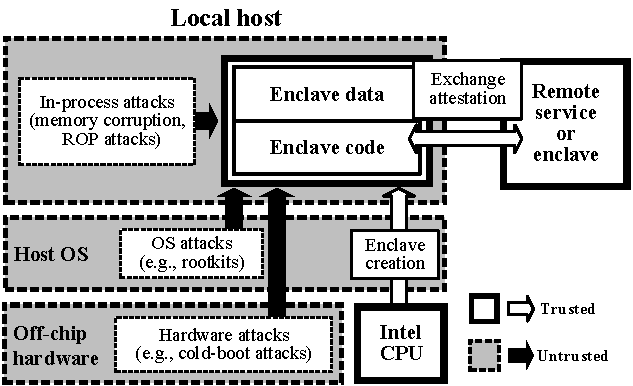
\includegraphics[width=.5\linewidth]{sgx.pdf}
\caption{The threat model of \sgx{}. \sgx{} protects applications
from three types of attacks:
in-process attacks from outside of the enclave,
attacks from OS or hypervisor, and attacks from off-chip hardware.}
% Red (dark) boxes are untrusted components and green (light) boxes are trusted.}
%For each enclave, \sgx{} establishes the chain of trust from the \intel{} CPU.
%Enclaves across physical machines or even infrastructures can remotely attest the integrity of execution, using the signatures generated and signed by the CPU.
%Green (light) boxes and arrows represent the trusted components and operations, and red (dark) boxes and arrows represent the otherwise.
\label{fig:sgx-threats}
\end{figure}

\paragraph{How much functionality to pull into the enclave?}
At one extreme, a library OS like Haven~\cite{baumann14haven} pulls most
of the application-supporting code of the OS into the enclave.
On the other extreme, thin ``shim'' layers, like SCONE~\cite{osdi16scone} and Panoply~\cite{shinde17panoply} 
wrap an API layer such as the system call table.
Pulling more code into the enclave increases the size of the TCB,
but can reduce the size and complexity of the interface, and attack surface, 
between the enclave
and the untrusted OS.

The impact of this choice on performance
largely depends on two issues. First, entering or exiting the enclave 
is expensive; if the division of labor reduces enclave border crossings, 
it will improve performance.
The second is the size of the Enclave Page Cache (EPC),
limited to 128MB on version 1 of SGX.
If a large supporting framework tips the application's working set size
past this mark, the enclave will incur expensive swapping.


\paragraph{Shielding complexity.}
SGX hardware can isolate an application from an untrusted OS, but 
SGX alone can't protect an application that  requires
functionality from the OS.  {\em Iago attacks}~\cite{checkoway13iago}
are semantic attacks from the untrusted OS against the application, where an unchecked system call return 
value or effect compromises the application.
Iago attacks can be subtle and hard to comprehensively detect, at least with the current
POSIX or Linux system call table interfaces.

Thus, any SGX framework must provide some {\em shielding} support, to 
validate or reject inputs from the untrusted OS.  
The complexity of shielding is directly related to the interface complexity:
inasmuch as a library OS or shim can reduce the size or complexity of the 
enclave API, 
the risks of a successful Iago attack are reduced.

\paragraph{Application code complexity.}
Common example applications for SGX in the literature 
amount to a simple network service running a TLS
library in the enclave, putting minimal demands on a shim layer. 
Even modestly complex applications, such as the R runtime and a simple
analytics package, require dozens of system calls providing wide-ranging functionality, 
including \syscall{fork} and \syscall{execve}.
For these applications, the options for the user or developer become: 
(1) modifying the application to require less of the runtime; (2) opening and shielding more 
interfaces to the untrusted OS; (3) pulling more functionality into a shim or a library OS.
The goal of this paper is to provide an efficient baseline, based on (3),
so that users can quickly run applications on SGX, and developers can 
explore (1) or (2) at their leisure.

\paragraph{Application partitioning.} An application can have multiple
enclaves, or put less important functionality outside of the enclave.
For instance, a web server can keep cryptographic keys in an enclave,
but still allow client requests to be serviced outside of the enclave.
Similarly, a privilege-separated or multi-principal application might create a separate enclave for
each privilege level.

This level of analysis is application-specific, and beyond the focus of this paper.
%which is on running unmodified applications in enclaves.
However, partitioning a complex application into multiple enclaves
can be good for security. In support of this goal,
\graphenesgx{} can run smaller pieces of code, such as a library, in an enclave, as well as
coordinate shared state across enclaves.

%* Partitioned vs. unpartitioned app?

%** Right choice depends a lot on whether the app has multiple principals or security concerns.

\begin{comment}
\fixmedp{Did a first cut at 2.2; needs to integrate the figure (or drop it).  I didn't know what to write for 2.3 yet.  I left the old text below for now (if there is anything you really want to save), but it needs to go away}

\subsection{Open Challenges}

\fixmedp{Here, I would give a taste of some of the issues we solve and why they are hard, like dynamic loading (and maybe fork or IPC).  Keep it short, a few paragraphs.}
\end{comment}

%\begin{figure}[t!]
%\centering
%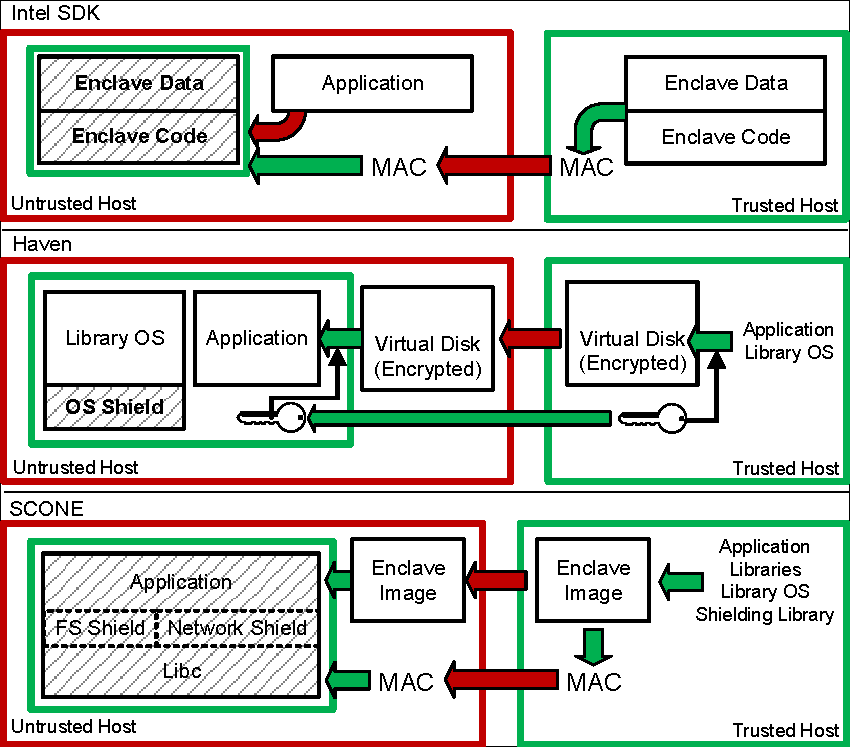
\includegraphics[width=\linewidth]{figures/sdkvslibos.pdf}
%\caption{Comparison of the code integrity model among different \sgx{} frameworks, including the \sdk{}, \haven{} and \scone{}.}
%%Green (light) boxes and arrows represent the trusted components
%%and operations, and red (dark) boxes and arrows represent the otherwise.
%%Patterned blocks represent the code and data included in the initial measurements of the enclaves.}
%\label{fig:sdkvslibos}
%\end{figure}


\begin{comment}
\subsection{\sgx{} shielding systems}
\label{sec:background:shielding-systems}




The current \sgx{} shielding systems, such as \haven{}~\cite{baumann14haven}, \scone{}~\cite{osdi16scone}, and Panoply~\cite{shinde17panoply}, enforce end-to-end isolation to
legacy applications without partitioning.
A \sgx{} shielding system preserves the trusted computing base (TCB)
of an application, and further increases it with a shielding layer to defend against the untrusted OSes.
By avoiding application partitioning,
%model of quarantining an unmodified, COTS application in an \sgx{} enclave.
a shielding system minimizes the effort of reprogramming the applications for \sgx{} execution, often with recompilation or packaging the binaries in an encrypted enclave.
%to merely recompiling or packaging the application code before signing it off for enclave execution.
%These \libos{}es internalize OS features into the enclave, to maintain a fixed-size,
%narrow interface to the untrusted host OSes.
%Porting applications using a \sgx{} \libos{} is vastly different from the programming model of \sdk{}---no programming effort is needed when porting with a \sgx{} \libos{}, and applications are isolated without partitioning.
In the following paragraphs, we compare the current shielding systems with the \graphenesgx{} approach.

\haven{}~\cite{baumann14haven} uses a \libos{} called \drawbridge{} in each enclave
to shield a single-process \emph{Windows} application from the untrusted host OS.
\haven{} absorbs the implementation of system APIs (i.e., Win32 APIs) from the host OS,
%\haven{} uses \drawbridge{}~\cite{porter11drawbridge} as the backbone of its enclave infrastructure, 
and exports a narrow enclave interface on which untrusted inputs are carefully filtered to defend against the Iago-type attacks.
Adding a \libos{} to each enclave causes a bloat of TCB---for \haven{}, the size of a \libos{} binary and shielding layer is \roughly{}200MB.
\haven{} has to establish the trust and integrity in all these binaries loaded into an enclave. Except that the shielding layer is a part of the enclave since its creation, \haven{} enforces the integrity of both the \libos{} and the isolated application,
by storing all binaries on an encrypted virtual disk and relying a remote, trusted server to provision the key for decryption.
\haven{} builds a trusted path from a remote server to local cloud machines,
to securely bootstrap application execution inside the enclaves.
%Other minor comparison between \haven{} and this work: the development and evaluation of \haven{}, at publication, is based on a simulated architecture.
%On the contrast, \graphenesgx{} is a released open-source platform, tested by many developers from institutes and corporations. \fixme{maybe bring up TCB?}



\scone{}~\cite{osdi16scone} isolates Linux micro-services in enclaves as a container-like environment.
After a brief attempt of building a \libos{} like \haven{},
\scone{} chooses a different approach of shielding the system API usage in applications, by designing shielding strategies based on each API.
\scone{} stacks the application on top of file-system and network shielding libraries, and extends a standard library C (musl~\cite{musl}) to securely exit the enclave for system calls.
Within the \sgx{}-aware Libc, \scone{} carefully filters the inputs from the host system calls, as the defend against known Iago attacks.
For instance, \scone{} ensures that pointers given to and returned by a host system call will point to addresses outside the enclave,
to prevent the host OS to manipulate pointers and cause memory corruption in the enclave.
\scone{} also authenticates or encrypts file or network streams
based on configurations given by the developers.


%The \libos{} implementation in \scone{} is based on musl~\cite{musl} and LKL (Linux kernel library)~\cite{lkl}.
%The design of a SCONE enclave (or Secure Container) has similarity
%with a basic block of \graphenesgx{}:
%they both validate input files based on cryptographic methods, and are fully configurable at a per-file basis.
%However, \graphenesgx{} supports a more complete set of Linux system APIs.
%The APIs that \graphenesgx{} especially contributes over \scone{} are the Linux multi-process APIs, including copy-on-write {\tt fork()}, {\tt exec()}, signals, and system V IPC (message queues and semaphores).

Panoply~\cite{shinde17panoply} further reduces the TCB of a shielding system over the SCONE approach, by excluding both a \libos{} and \libc{} from enclaves.
Instead, Panoply uses a shim layer shielding a portion of the POSIX API. The shim layer yields about 20 KLoC as its TCB (trusted computing base), which is much smaller than libc and/or a library OS.
% in other shielding systems.
As Panoply delegates the libc functions outside the enclave, its shim library defends the supported POSIX API,
including 91 {\em safe} functions and 163 {\em wild (unsafe)} functions.
Panoply also supports multi-process API including \fork{}, \exec{}, signaling, and sharing untrusted memory with inline encryption.
Compared to \graphenesgx{}, Panoply has made some different design decisions in supporting multi-process API,
including supporting fork by copying memory on-demand with statically determining memory access,
and using secured messaging for inter-process negotiating instead of coordinating over an encrypted RPC stream.




\subsection{Comparison and security implications}

\fixme{need to drop the SDK discussion, revisit the security claims, and discuss Iago attacks in details.}

Figure~\ref{fig:sdkvslibos} shows the comparison between \haven{}, \scone{}, Panoply, and \graphenesgx{}.
%The \sdk{} model uses a static MAC of the enclave code and data, given to the \sgx{} driver for bootstrapping the isolated execution.
The \haven{} model only initiates enclaves with the OS shield layer,
which unpacks the enclave binaries from a virtual disk---decrypted using a provisioned key.  
The \scone{} model extends the \sdk{} model---it statically links the application binaries with the shielding library, creating a static enclave image verifiable by its MAC. The \sdk{} and \scone{} model retain more flexibility in deploying and integrating \sgx{} enclaves by focusing on the code integrity rather than encryption.

The key concerns that affects users choosing among these solutions are {\bf trusted computing base (TCB) size} and {\bf attack surface}.
However, since all these solutions are based on different design decisions, assumption and requirements, the comparison of TCB size and attack surface is often imprecise and inconclusive.

\paragraph{TCB size.}
Most studies measure the TCB size of a system by the total LoC (lines of code) written for all the trusted components, or the size (in bytes) of all the trusted binaries.
The comparison of TCB size is only meaningful when two systems have comparable system features,
and are order-of-magnitude different in term of LoC or binary size.
For instance, the comparison of TCB size between \haven{} and \scone{} is never an apples-to-apples comparison.
The implemented system features and personalities
in these two systems are fundamentally different, and \haven{} supports a much larger fraction of Windows features than the fraction of Linux features supported by \scone{}.

We argue that the only occasion that the reduction of TCB size
can be convincingly demonstrated is when a design has partitioned a system into isolated components,
or removed unreachable execution paths.
For instance, the \sdk{} promotes application partitioning for \sgx{};
it requires additional partitioning effort but is effective for confining the TCB size.
By statically linking the application binaries
with the shielding layers and standard C library, \scone{} offers more opportunities in stripping the Libc and shield code of unused APIs, and thus reducing its TCB size.



\paragraph{Attack surface.}

Most studies estimate the severity of having an attack surface by the size of interface to the trusted and untrusted components.
The experience of \scone{} provides an important insight for estimating attack surface: the narrowness of interface is not proportional to the difficulty of defending against incoming attacks.
An interface overloaded with too many features or semantics can become a major source of vulnerabilities.

%\subsection{The \graphene{} Library OS}
%
%\graphene{}~\cite{tsai14graphene} introduces a \libos{} design that supports
%both single-process and multi-process Linux applications,
%but retains a narrow host interface (43 functions) as a vantage point for enforcing security isolation.
%The main contribution of \graphene{} is an distributed implementation of the POSIX namespace coordination,
%to support Linux multi-process abstractions across \libos{} instances.
%All the multi-process abstractions in \graphene{} is implemented using simple pipe-like RPC streams,
%without relying on any host memory sharing support.
%Based on this design, \graphene{} can easily isolate mutually untrusting applications,
%by blocking the RPC streams between unrelated applications.
%
%
%
%The design decisions made by \graphene{} are important keys to the \graphenesgx{} framework.
%First, the host interface contains mostly internal abstractions, and three external ones including files, network connections, and RPC streams.
%The simplicity of the host interface facilitates shielding the \libos{}
%from risky OS interaction.
%Moreover, \graphene{} implements multi-process abstractions across instances without memory sharing.
%\graphenesgx{} can rely on the distributed POSIX implementation
%to support multi-process applications across multiple enclaves, by coordination over validated RPC streams.


\end{comment}




\section{Minimizing Hit Latency}
\label{sec:dcache}

This section describes
%The first category of optimizations we describe are 
algorithmic improvements to the dcache hit path.  
In the case of a cache hit, one of the most expensive operations
is checking whether 
a process's credentials permit the process to search
the path to a \dentry{} top-down (called a {\bf prefix check}).
This section shows how the hit latency can be significantly reduced
%(by 26\% in our \microbench{}s)
by caching prefix check results.
%this particularly expensive data structure traversal in the common case.
This section explains the optimization, how it is integrated into the existing Linux directory cache 
framework, how these cached results are kept coherent with other file system operations,
and how we use path signatures to further accelerate lookup.


% Should we justify the cost of the search component with measurement?

\subsection{Caching Prefix Checks}
\label{sec:dcache:prefixcheck}

\begin{figure}[t!]
\centering
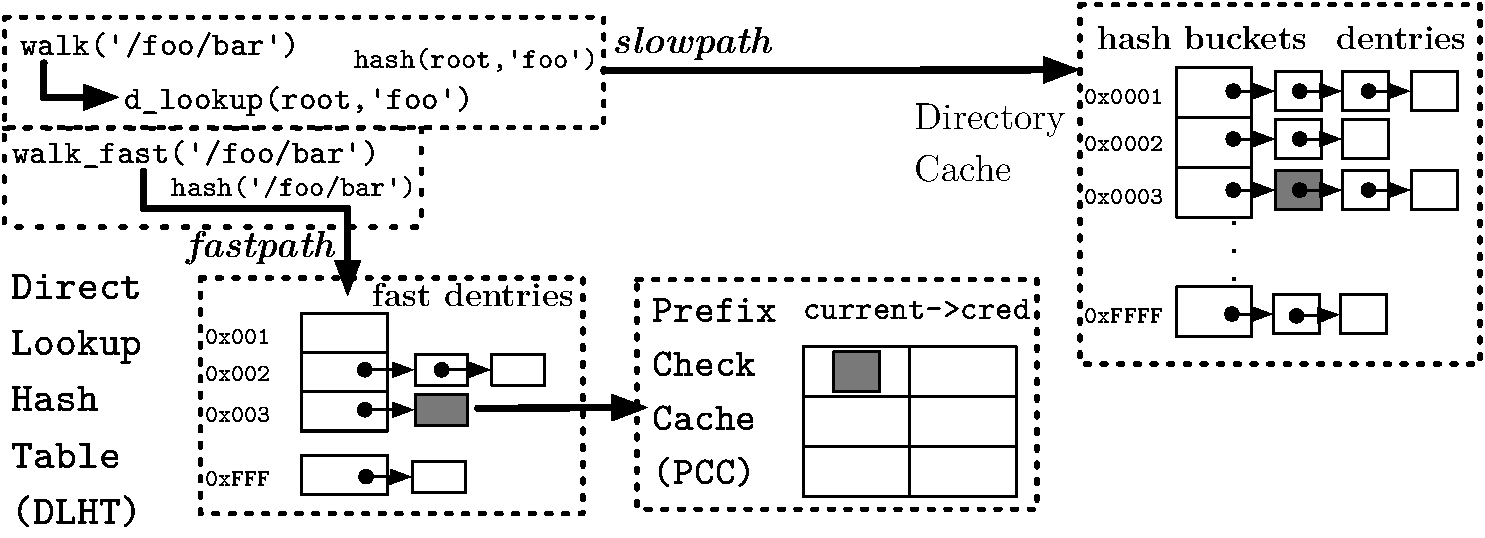
\includegraphics[width=4in]{dcache/figures/dcache-structure.pdf}
\footnotesize
\caption[Optimized Linux directory cache structure.]
{Optimized Linux directory cache structure. \dentries{} are chained in hash buckets. To index the hash bucket for a target \dentry{}, the original lookup routine {\tt d\_lookup} uses a hashing function with key as a combination of the pointer to parent directory and file name ({\em slowpath}).
Our {\em fastpath} hashes the full canonical path of target file to look up the \dentry{}
in the Direct Lookup Hash Table,
and checks the per-credential Prefix Check Cache.}
\label{fig:dcache}
\end{figure}

%\fixmedp{update the picture with new tables}
Like many Unix variants, Linux stores cached path-to-inode mappings (\dentries{}) in a hash
table (\S\ref{sec:background:dcache}).  This hash table is keyed by a combination of 
the virtual address of the parent \dentry{} and the next path component string, illustrated in
Figure~\ref{fig:dcache}.  
Virtual addresses of kernel objects do not change over time and are identical across processes.
%Each path component is checked for search permission in a top-down fashion,
%which we call a {\bf prefix check}.
%For instance, to look up component {\tt alice} in {\tt /home/alice/foo.txt},
%the kernel would take the virtual address of the \dentry{} for {\tt /home}, 
%and hash it with the string ``alice'' in order to find the bucket to search
%for the \dentry{} mapping ``alice'' to an inode, in order to check search permission on 
%the {\tt alice} directory.
%The latency of a prefix check, and thus a lookup, 
%grows linearly with the number of path components in the prefix.

In practice, prefix checks have a high degree of spatial and temporal locality,
and are highly suitable for caching,
even if this 
means pushing some additional work onto infrequent modifications of the directory structure (e.g., {\tt rename} of a directory).
RCU already makes this trade-off (\S\ref{sec:background:dcache}).

%Application file access patterns exhibit substantial temporal and spatial locality.
%Moreover, lookups (i.e., reads of the directory hierarchy)
%are vastly more common than modifications of the directory structure (e.g., {\tt rename} of a 
%non-empty directory) or permission changes within the directory structure (e.g., {\tt chmod} or {\tt chown} of a directory).


%% dp: Maybe cut this. Kind of meh
%% Caching prefix checks is analogous to caching access permissions along with 
%% virtual-to-physical translations in a hardware 
%% translation lookaside buffer (TLB). 
%% For instance, each level of an x86 page table encodes access permissions 
%% (e.g., read, write, execute, and user/kernel).  As the hierarchy grows deeper with larger address spaces
%% and hardware virtualization support~\citep{intel10, nestedpagetables}, 
%% needless loads can be elided.

%Linux's use of RCU already makes this trade-off (\S\ref{sec:background:dcache}).

In order to cache prefix check results, we must first decouple 
{\em finding} a \dentry{} from the prefix check.
We added a second, system-wide hash table exclusively for finding a \dentry{}, called the {\bf direct lookup hash table (DLHT)}.
%which only stores recently-accessed \dentries{},
%of \fixmedp{directories?}
The DLHT stores recently-accessed \dentries{}
hashed
by the full, canonicalized path.
A \dentry{} always exists in the primary hash table as usual,
and may exist in the DLHT.
The DLHT is lazily populated, and entries can be removed for coherence
with directory tree modifications (\S\ref{sec:dcache:rename}).

\begin{comment}
\fixmedp{proposed change; measure impact}
\fixmetsai{no done yet, and not sure about the impact. In general, if a file (a leaf) is constantly accessed, there is benefit to add it to DLHT.
Also a dentry found on fastpath means all of its ancestors have passed prefix checks, so if only directories stored, we still have to do one more check.}
%We limit the DLHT to directories because only directories 
%can be in a prefix.  Our lookup algorithm always does a second hashtable
%lookup in the primary hashtable for the final path component.
\end{comment}

Each process caches the result of previous prefix checks
in a {\bf prefix check cache} (PCC), associated with the process's credentials
(discussed further in \S\ref{sec:dcache:cred}), which can be shared among processes
with identical permissions.
The PCC is a hash table that caches dentry virtual addresses 
and a version number (sequence lock), used to detect stale entries (\S\ref{sec:dcache:rename}).
When a prefix check passes, indicating that the credentials are allowed to access the \dentry{}, 
an entry is added to the PCC; entries are replaced according to an LRU policy.
A miss in the PCC can indicate a permission denied
or 
%, which we believe is an uncommon case, or, more commonly,
that the permission check has not executed recently.

%The PCC is a hash table to quickly check if a dentry{} is recently prefix-checked.
%% dp: Meh
\begin{comment}
For simplicity, we implemented a set associative cache, resembling the design of a L1 cache in CPU, but a more sophisticated data structure such as
{\em Cuckoo hashing}~\citep{cuckoo04} can be even more efficient. 
\end{comment}
%lookup and insertion time asymptotically constant.
%The PCC is initially 64 entries, and in our current prototype doubles in size, up to a configurable
%maximum size,
%each time it exceeds a 50\% load factor.  
%If the maximum size and load factor are exceeded
%\fixmedp{implement}  





%% We changed the kernel path hashing strategy to 
%% simply hash the entire canonicalized path, rather than hash 
%% the virtual address of the parent \dentry{} and the next path component.
%% Thus, given any path, the kernel can directly look up the \dentry{} 
%% without walking the entire directory hierarchy.

%% We create a separate hash table, which we call a {\bf direct lookup hash table (DLHT)}.
%% When a \dentry{} is being hashed,
%% it is inserted into both \dcache{} hash table and fast lookup hash table,
%% using their hashing functions respectively.


%% Our {\bf first design} includes placing a {\bf prefix check cache (PCC)} into each \dentry{},
%% %which stores the results of up to \prefixcheckcachesize{} prefix checks,
%% %for \prefixcheckcachesize{} credentials who have most recently look up the \dentry{}.
%% which stores limited amount of prefix checks for credentials who have most recently looked it up.
%% Each cached prefix check is stored using one 64-bit word: 63 bits for a credential identifier
%% and one bit for the prefix check result.
%% However, adding prefix check cache largely increases the size of each \dentry{},
%% thus it will compress the total number of \dentries{} that can be loaded into RAM.
%% The prefix check caches in the most popular \dentries{}
%% will be frequently replaced
%% and have a high cache miss rate,
%% while the other ones can remain underused. 
%\fixmedp{If time, figure out how compact we can reasonably make this}
%The credential identifier, detailed in \S\ref{sec:dcache:selinux},
%represents the process's user id, group membership, capabilities, or any other credentials 
%that could have influenced the prefix check results.
%If any process attributes change that could influence a prefix check, the process must also change
%its credential identifier.


%% To improve space efficiency and cache miss rate of popular \dentries{},
%% our {\bf second design}
%% instead places a {\bf \dentry{} lookup table (DLT)}
%% into the Linux {\tt cred} structure (explained in section~\ref{sec:dcache:cred}).
%% The \dentry{} lookup table is a hash-based set-associative table,
%% and each of its entry contains two 32-bit words:
%% one for storing the lower 9th-40th bit of \dentry{} pointer that has been prefix-checked,
%% and the other for caching the sequence counter of the \dentry{} to determine whether it has been updated.
%% %(0 represents the prefix check has failed).
%% For each credential
%% we initially allocate a DLT with \lookuptablesize{} entries split in \lookuptableway{} ways.
%% The table can be dynamically extended if a credential is looking up more \dentries{},
%% and needs to cache more prefix check results. 

%% dp: worth exploring...
\begin{comment}
Thus, given any path prefix, the kernel
has a {\em fastpath} that directly looks up the prefix 
in the DLHT.  The fastpath case looks up the immediate
parent in the DLHT, checks cached permission for the entire prefix 
(described next), and then looks up the file itself in the primary hashtable.
If the fastpath fails, the code falls back on the original Linux lookup algorithm,
using the primary hashtable exclusively, and traversing components one at a time.
\end{comment}

Thus, given any path, the kernel
has a {\em fastpath} that directly looks up the path
in the DLHT.
If the fastpath hits in the DLHT,
the \dentry{} is then looked up in the process's PCC.
If a PCC entry is found and the version counter matches 
the cached counter, the cached prefix check result is used.
%with the same pointer is found and the sequence counter matches with the the \dentry{}, the results of the cached prefix check are used.
If the fastpath lookup misses in the DLHT or PCC, 
or the version counter in the PCC entry is older than the \dentry{}, 
the code falls back on the original 
Linux lookup algorithm (the {\em slowpath}),
using the primary hashtable exclusively and traversing one component at a time.

%\fixmedp{Chia-che, check this}
In the case of a relative path, such as {\tt foo/bar} under directory {\tt /home/alice},
we effectively concatenate the relative path and the path of the current working directory.
To implement relative paths, Linux already stores 
a pointer to the {\tt dentry} of the current working directory
in each process descriptor ({\tt task\_struct}).
Rather than {\tt memcpy} the strings, we store the intermediate state of the hash function 
in each {\tt dentry} so that hashing can resume from any prefix.

%\fixmedp{Chia-che check this; we should handle these cases; hacks are ok}
%\fixmetsai{revisited}
The current design includes two very infrequent edge cases.
First, a \dentry{} could be freed and reallocated with stale PCC entries.
We detect this case by initializing newly allocated \dentries{} with
%the maximum version number,
a monotonically increasing version number,
allowing PCC entries to detect staleness across reallocation.
Freeing a \dentry{} removes it from the DLHT.
Second, a version number can wrap around after every $2^{32}$ initializations of new dentries or
renames, chmods, or chowns
of non-empty directories; 
our design currently handles wrap-around by invalidating all active PCCs.
%entries less than $2^{31}$
%our design uses a garbage collector to scan all existing PCCs to gradually eliminate stale entries. \fixmetsai{need to implement}

\begin{figure}[t!]
\centering
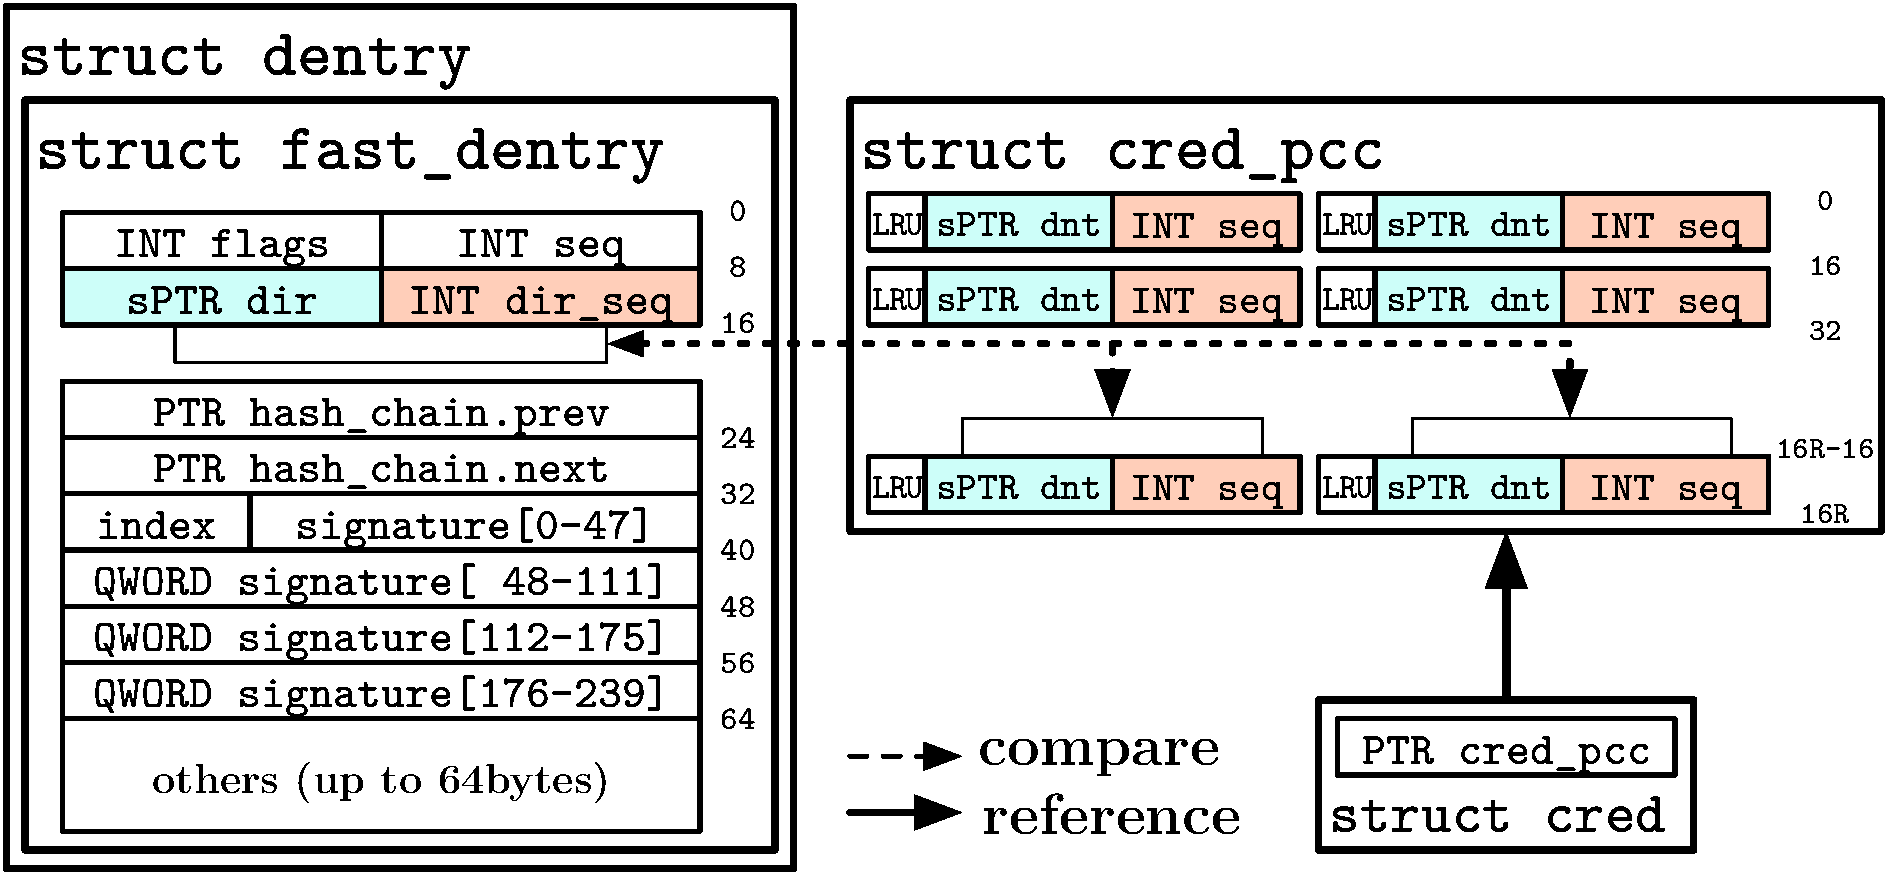
\includegraphics[width=4.5in]{dcache/figures/dcache-data_structure.pdf}
\footnotesize
\caption[Data structures added in Linux for directory cache optimization]
{Data structures added for fast directory cache lookup. To support {\em fastpath} lookup, we add a 88-byte fast dentry structure to the original \dentry{} and a variable-sized PCC structure into {\tt cred}. 
%% dp: meh
%Both structures are aligned to 64-byte cacheline to make lookup cache-friendly.
}
\label{fig:dcache-data-structure}
\end{figure}

Figure~\ref{fig:dcache-data-structure} illustrates the modifications 
to the Linux \dentry{} structure.  The {\tt fast\_dentry}
stores the signature, flags, a sequence count, a mount point,
lists for managing deep directory entries (\S\ref{sec:readdir:deep}),
and a list ({\tt hash\_chain}) for adding the fast\_dentry to a DLHT bucket.
The PCC is added to the kernel credential structure ({\tt struct cred}), %discussed in \S\ref{sec:dcache:cred}),
and stores a tunable number of tuples of \dentry{} pointers and sequence numbers;
the system is evaluated with a PCC of \PCCsize{}.
Because the highest and lowest bits in each \dentry{} pointer are identical,
the PCC only stores the unique pointer bits (8--39 in x86\_64 Linux) to save space.

%% SOSP Space
%% Although caching prefix checks is straightforward as described thus far,
%% this change 
%% causes ripples through the rest of the code, creating several additional challenges, such as 
%% keeping the cache coherent with modifications.
%% The following subsections address these challenges in the course of 
%% explaining the implementation in more detail.

%\fixmedp{Should we talk about signatures here? I'm tempted to push this to another subsection.}
%\fixmedp{Later: Make sure we explain how we shoot down entries somewhere}

% Order of subsections:
%% Credential IDs and generalization
%% Shootdown
%% Signatures and collisions
%% Special cases



%% \fixmedp{Move down...}
%% Permission caching is a simpler approach to determine file permission
%% than merging access rights of all parent directories.
%% The merging approach is used by related works like DLFS~\citep{lensing13dlfs},
%% which can only resolve permission based on
%% credentials of users and groups.
%% It cannot support more sophisticated access,
%% such as SELinux or AppArmor.
%% On the other hand, The permission caching approach requires no effort of
%% implementing permission merging,
%% thus it is able to support any access control,
%% including SELinux and AppArmor.
%% More details of access control support is discussed in section~\ref{sec:dcache:selinux}.

%% Using permission caching, our lookup method can calculate access right of
%% entering all parent directories to access target file,
%% without any sophisticated merging logic.
%% For every security credential, the access right is calculated by forcing
%% the lookup routine to fall back to the slow path at the first access on any file.
%% Because the slow path shares the exactly same logic as the original component-based lookup in Linux kernel,
%% it can rely on the existing routine of access right checking to determine permissions. 
%% This section will discuss more details about permission caching for fast directory cache lookup.

\subsection{Coherence with Permission and Path Changes}
\label{sec:dcache:rename}

When permissions on a directory or the directory structure are changed, such as with {\tt chmod} or {\tt rename},
any cached prefix checks that include this directory must be invalidated.
Our design  ensures the safety of concurrent lookups and changes by 
invalidating relevant PCC and DLHT entries before a change to the hierarchy,
preventing stale slowpath lookups from being re-cached, and leveraging VFS-level synchronization
to ensure correct slowpath behavior.
  
First, we ensure that a fastpath lookup cannot complete with stale data after a change to the directory structure.
Before a mutation, such as a {\tt rename} or {\tt chmod}, the operation 
must recursively walk all children in the \dcache{} 
and increment the {\tt fast\_dentry} version counter ({\tt seq}). % (steps a1--a4).  
The {\tt fast\_dentry} version counter is used by each process's PCC to detect changes to cached prefix checks on a lookup; % (step b2);
incrementing this version counter invalidates all PCC entries for that \dentry{} without directly modifying
each PCC.  
Changes to the directory structure (e.g., {\tt mount} and {\tt rename}) 
also remove \dentries{} under the old and new path 
from the direct
lookup hash table (DLHT).
PCC and DLHT entries are lazily repopulated on the slowpath.
%These paths can be lazily added back to the DLHT on the slowpath.

Second, we ensure that the results of a  stale slowpath lookup cannot be re-added to the DLHT or PCC by using an atomic, global sequence counter ({\tt invalidation}).
The sequence counter is read before and after a slowpath traversal; results are added to the DLHT and PCC only 
if the counter has not changed, implying no concurrent shootdowns.

Third, we use VFS-level synchronization to ensure that slowpaths synchronize correctly 
with the mutation. 
As an example, {\tt rename}
%%Before the rename begins, our code acquires the 
%%  {\tt invalidation\_lock}, invalidates the relevant children, 
%% acquires the appropriate 
%% VFS-level locks, and then releases the {\tt invalidation\_lock}.
%Rename has stricter requirements to ensure atomicity.
%In the case of {\tt rename}, 
acquires both
a global {\tt rename\_lock} sequence lock, along with per-\dentry{}
locks on the old and new parent directory.
When the {\tt rename\_lock} is held for writing, all lookups on the slowpath 
(i.e., the current Linux code)
must lock each \dentry{}
in a hand-over-hand fashion from the root (or current working directory, for relative paths) 
to the target child.
The locks on target \dentries{} obstruct the hand-over-hand traversal until the rename completes.
The {\tt invalidation} counter prevents caching the results of slowpath lookups that already passed 
this point before the \dentry{} locks were acquired.
%The {\tt rename\_lock} is held until all relevant DLHT entries are evicted,
%and our fastpath traversal is also retried if a concurrent rename is detected by the {\tt rename\_lock}'s sequence count.
%In the current Linux VFS, and our {\em slowpath}, 
Our implementation follows the VFS's existing locking discipline to avoid deadlocks;
it adds version counters that detect inconsistencies and falls back on the slowpath.
Thus, 
relevant PCC and DLHT entries are invalidated before the rename begins, blocking the fastpath;
slowpath traversals will block until the rename is complete
and the per-\dentry{} locks are released;
and a sequence counter ensures that only slowpath traversals that observe the new paths can repopulate the DLHT and PCC.



%% SOSP Space
%% Our \dcache{} design deliberately pushes some additional work onto the uncommon cases of 
%% directory permission changes or changes to the directory structure itself, in order
%% to accelerate frequent lookups.

%% dp: SOSP Space cut
%This is illustrated in Figure~\ref{fig:invalidation}.
%In order to invalidate PCC entries that refer to this directory's children, 
%a permission change operation 
%this choice avoids computing and updating
%prefix checks that will not be used.

%% dp: SOSP Space cut
%% Michael finds this hard to follow
\begin{comment}
\begin{figure}[t!]
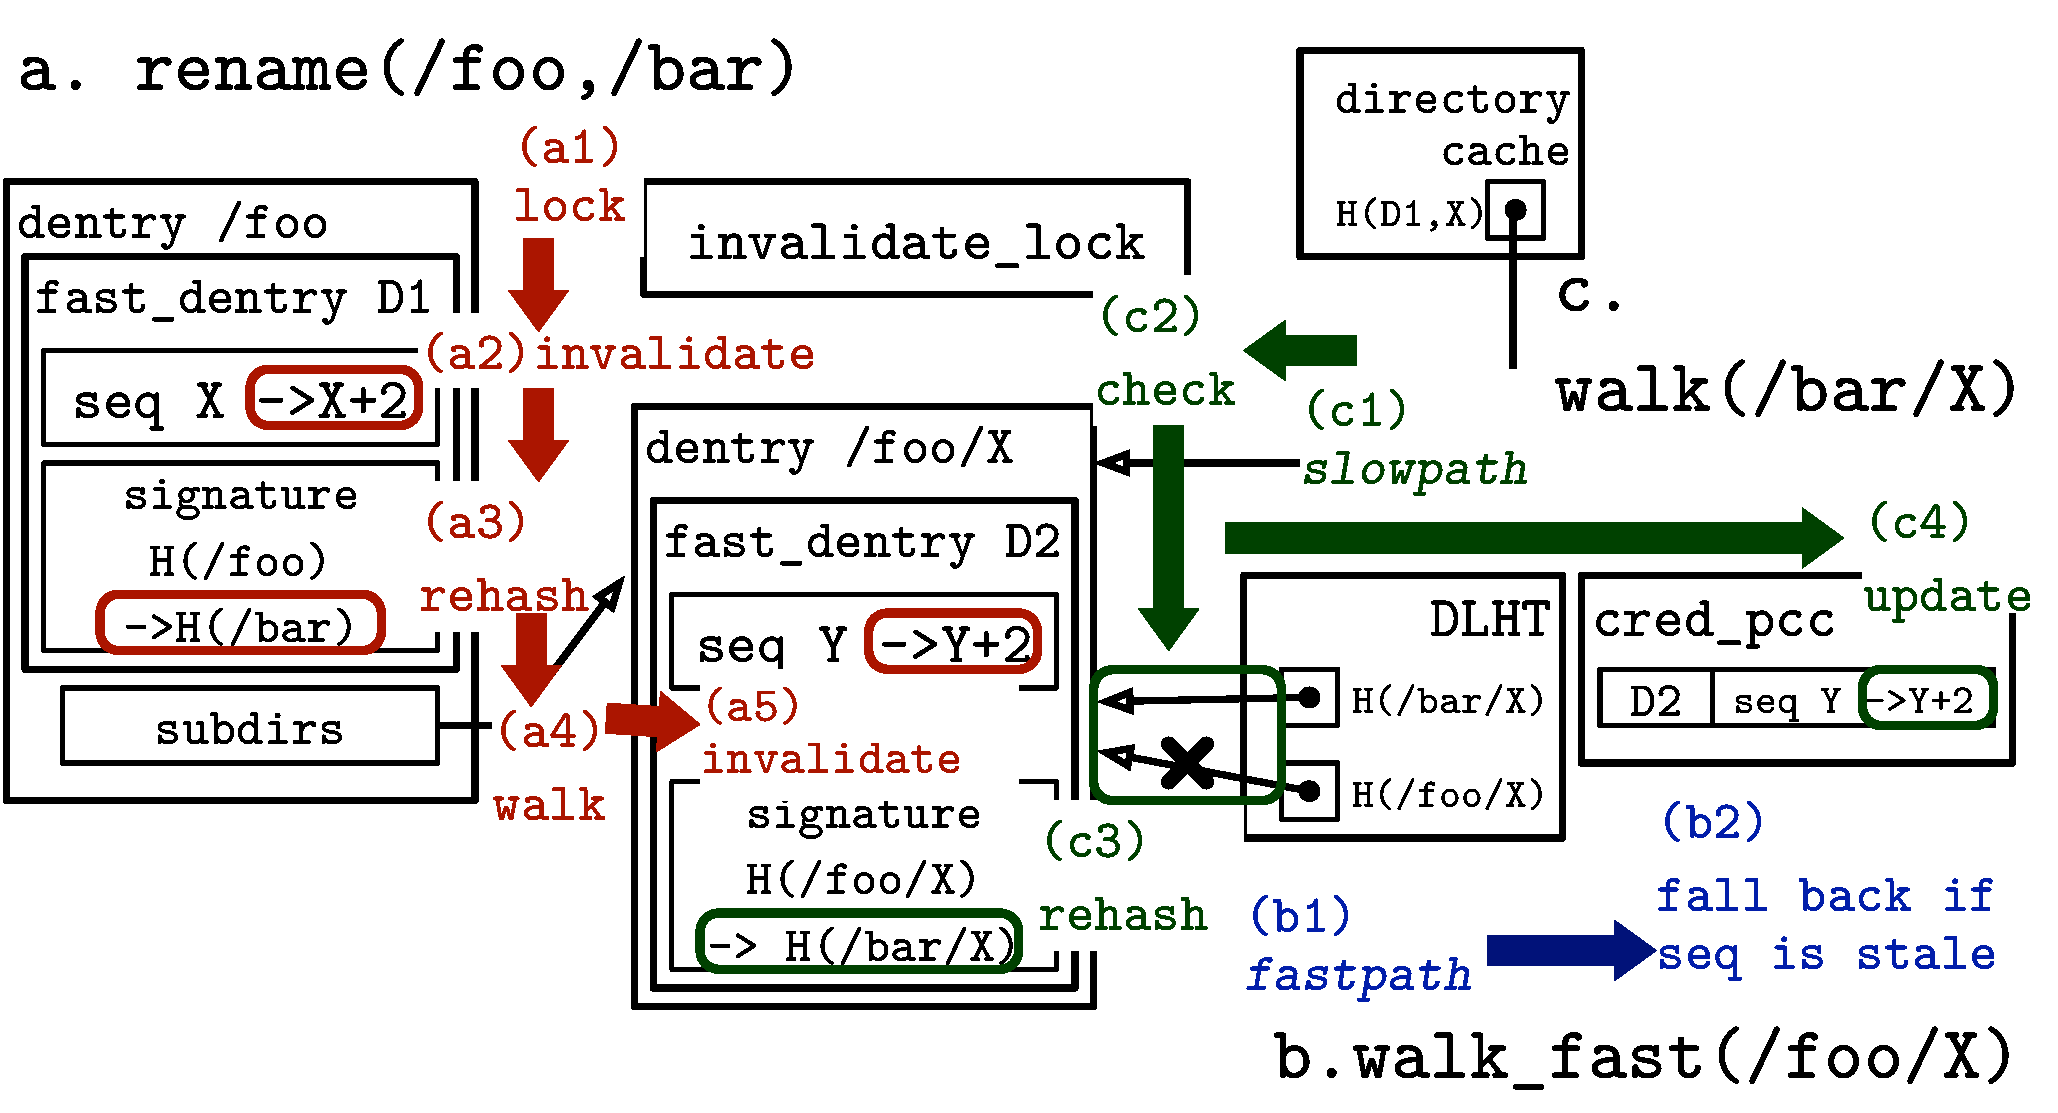
\includegraphics[width=1.0\linewidth]{dcache/figures/invalidation.pdf}
\vspace{-15pt}
\footnotesize
\caption{Procedure of updating directory trees for {\tt rename}/{\tt chmod} system calls.
The procedure {\color{red} (a)} invalidates the \dentries{} in all PCCs by incrementing the sequence counters {\color{red} (a2)}. The path will be rehashed. {\color{red} (a2)}.
The procedure then walks all child \dentries{} {\color{red} (a4)} and invalidate them {\color{red} (a4)} (but no rehashing).
A global lock will be held for coherence {\color{red} (a1)}.
If later the old path is looked up on the {\em fastpath} {\color{blue} (b)}, the found \dentry{} {\color{blue} (b1)} has a different sequence counter with the current PCC {\color{blue} (b2)}, thus revalidation is needed.
The forced {\em slowpath} {\color{OliveGreen} (c)} will look up the new path hierachically {\color{OliveGreen} (c1)}, check if the global lock is held {\color{OliveGreen} (c2)}, rehash signature {\color{OliveGreen} (c3)} and finally update the PCC {\color{OliveGreen} (c4)}.  }
\label{fig:invalidation}
%\vspace{-10pt}
\end{figure}
\end{comment}

%% Permissions changes are kept coherent  by 
%% causing fastpath traversals to retry on the slowpath when relevant \dentries{} change.
%% Slowpath traversals will always see a correct
%% view of the directory hierarchy via standard VFS-level synchronization.
%% Once a permission change is applied to a directory, the child version numbers are incremented
%% recursively.  
%% Once these changes are applied, any fastpath lookup will notice the difference in version numbers
%% between the child \dentry{} and the PCC entry, and retry the prefix check.

%% There is a brief window between the permission change of a parent and the version number change to a child.
%% A fastpath traversal during this time is equivalent to executing just before the permission change, which we consider acceptable, as no additional permissions can be acquired
%% and this window is quite short.
%% Similarly, a slowpath lookup  can start before the permission change, 
%% see the old value, and complete just after a permission change.
%% We prevent slowpath lookups from recreating potentially stale PCC entries
%% values by using a global sequence lock ({\tt invalidation\_lock}).



%We also increment the version counter on all children {\em before}
%the rename begins, and hold the
%Once a path is evicted from the DLHT, it 


%% dp: I think this is false
%A positive externality of this design is that the fastpath is never blocked by the {\tt rename\_lock} while {\em slowpath} can be forced to retry.  



\begin{comment}
\fixmedp{moved down from above (too early); dumped para here for now}
When directory structure changes, new prefix check result must be merged
onto every \dentry{} in the directory.
%In order to minimize the penalty on modifications,
We choose to lazily update the prefix check results, by preserving the original
component-based lookup algorithm as a fallback
while we temporarily block directly looking up the \dentries{} until the next access.


In the case of operations that influence a potentially-cached prefix check,
namely {\tt rename}, {\tt chmod}, {\tt chown},
and changes to security-relevant extended attributes,
we must clear the cached prefix check results on all descendants.
The way to clear cached prefix checks (or``to invalidate")
without actually zeroing any structures
is to force aging the sequence counters in the \dentries{}.
Specifically for {\tt rename}, we must also rehash all descendants in direct lookup hash table, because their canonical paths will also change.
\end{comment}

These recursive traversals shift directory permission and structure changes 
from constant time to linear in the size of the sub-tree.
As one example, 
%We found a simple recursive of the subtree to invalidate or rehash all descendants
%can be expensive in a deep directory.
 to {\tt rename} or {\tt chmod} a directory that has
10,000 descendants with at most depth of 4
takes roughly 330 microseconds to complete. 
%\fixmedp{updated numbers}
In the original Linux kernel, {\tt rename} and {\tt chmod} are nearly constant-time operations, and only take 4.5 and 1.1 microseconds.
A few applications, such as {\tt aptitude} or {\tt rsync},
rely on {\tt rename} to atomically replace a directory, 
but this is a small fraction of their total work % done even by these applications,
and orders of magnitude less frequent than lookups, making this a good trade-off overall.

\begin{comment}
The performance penalty for \fixmedp{app example} is \fixmedp{XX\%}.
\S\ref{sec:eval} includes more detailed measurements of these costs and the benefits of constant time lookup, indicating 
that this cost is acceptable.
\end{comment}
%We found a simple recursive walk of the subtree sufficient for our implementation, adding 12--16\% overhead 
%to {\tt chmod} of a directory---a very infrequent operation.
%To serialize readers, we hold the the parent dentry lock on the modified directory,
%which blocks the lookup slowpath until the modification is complete.
%Fast-path lookups which observe the old cached permissions are essentially serialized before the permission change.
%Subsequent executions of the slowpath will repopulate these caches.

\paragraph{Directory References.}
%\fixmedp{Chia-che check}
Unix semantics allow one to {\tt cd} into a directory, and continue
working in that directory after a subsequent permission change 
would otherwise prohibit further accesses.
%hold a reference to a file or directory
%after a permission check that 
%with an opened handle or the current working directory.
For instance, suppose a process is in working directory {\tt /foo/bar}
and {\tt foo}'s permissions change such that the process would not
be able to enter {\tt bar} in the future.
The process should be able continue to open files under {\tt bar}
as long as the process does not leave the directory or exit.
Similar semantics apply to open directory handles.
%Our solution must handle this use case without overriding the premission change.
%\fixmetsai{Don, I rewrote this part to reflect the current design. See if it make sense.}
In our design, such a permission change would ultimately result in a blocked PCC entry,
and a fastpath lookup would violate the expected behavior.
Our design maintains compatibility by
checking if the open reference is still permitted in the PCC.
If the PCC has a more recent entry that would prevent re-opening this handle,
the lookup is forced to take the 
the slowpath, and this stale result is not added to the PCC.

%If a PCC entry for {\tt /foo/bar} is inserted after {\tt /foo}'s permission change, future access to {\tt /foo/bar} will be allowed even after leaving or closing {\tt /foo}.
%This idiosyncrasy of isolating a working directory is supported by 

%If PCC no longer permits the current working directory or base handle, user can still look up paths inside the directory using 
 
%Our current prototype supports this idiosyncrasy by storing the version number
%of the current working directory as of the last {\tt cd};
%if the PCC entry is potentially newer, we only allow the slowpath 
%until the next {\tt cd}, for backward compatibility.
%We believe this is a case where the implementation has leaked into the interface,
%and a reasonable alternative in this situation would be to return an error, such as a stale file handle.

%% \paragraph{Updating Permissions.}
%% Access right of reaching a directory entry is determined by cached permissions
%% calculated in the slow path.
%% When the permission of a directory changes,
%% the kernel must invalidate all prefix check cache in every directory entry under the tree rooted at the directory,
%% to guarantee upcoming access to one of the directory entries be forced to
%% fall back to the slow path for recalculating the permission.

%% Invalidating of prefix check caches is required in two conditions:
%% \begin{compactitem}
%% \item Access permission of a directory is changed by {\tt chmod}, {\tt chown} or other system calls.
%% \item A directory is moved under a different parent directory.
%% \end{compactitem}
%% When invalidation is necessary, the kernel will traverse the whole tree of \dentries{} under the target directory,
%% and mark all \dentries{} as {\tt DENTRY\_INVALIDATED}.
%% If the {\em fastpath} finds a marked \dentry{}, it will fall back to component-based lookup,
%% which flushes the prefix check caches, unmark the \dentry{}, and revalidate the access permission. 

\begin{comment}
In order to mitigate the overhead on {\tt rename}, we push the work of rehashing onto the slowpath.
Because {\tt rename} also clears cached prefix checks,
any following lookup of the descendants
will be forced to fall back to hierarchical slowpath,
which can update direct lookup hash table complimentary.

Because we only invalidate \dentries{} at the operations like {\tt rename} and {\tt chmod}, and force consequential lookup to fall back to slowpath,
consistency of the directory structure is always maintained even if the operations happen concurrently.
The only exception is when a slowpath walk starts before a recursive invalidation happens,
and update a \dentry{} using wrong prefix check after it is invalidated,
the newly cached result will be counted as valid.
To prevent this scenario, we use a
global {\tt invalidate\_lock} sequence lock
to block prefix check caching
whenever an invalidation is in action.
This design is similar to the {\tt rename\_lock} used in the Linux kernel.

%\fixmedp{I see mount/umount as a case of shooting down entries.  I think the text below should be 
%merged in with rename discussion (although there are two sorts of shootdown)}
%\fixmetsai{The two kinds of shootdown is fundamentally different, because invalidation is to force lookup to fall back, but disconnection is to skip dentries while looking up.}

%Because dentries in our prototype are hashed by full path, rather than their parent pointer and file name,
%we must also recursively rehash all children and clear the prefix check cache when a 
%directory is moved.
%We find that this recursive traversal only increases the cost of a {\tt rename} by about 1\%.
% under a different directory.
%\fixmedp{Revisit if we save S4}

Because recursive invalidation can still be an major latency issue on some systems,
we provide an optimization to hide the overhead in the background
and remove penalty on the latency of operations that needs recursive invalidation.
The optimization use a kernel task to handle recursive invalidation
offline with spared CPU cycles.
The only caveat is that fastpath must be {\em disabled} when any invalidation is in process.

Finally, Unix specifies that when a file system is mounted over a non-empty directory,
all files or subdirectories under the directory will be disconnected from the system,
and become unavailable until the file system is unmounted.
We modify {\tt mount} to recursively invalidate all child \dentries{}.
When the file system is unmounted, these \dentries{} can be found again on slowpath and be resurrected for fast lookup.
\end{comment} 


%\paragraph{Disconnecting Directory Entries after Mounting.}
%Unix operating systems allow file system be mounted at any existing directories
%in the system.
%If the directory where mounting happens is not empty,

%In the original design, disconnecting \dentries{} is simple.
%Because all \dentries{} are looked up from their parents,
%disconnecting the root \dentry{} will automatically make all other \dentries{} in the tree unavailable.
%Our solution is to force a tree traversal to mark
%all \dentries{} under the tree as {\tt DENTRY\_DISCONNECTED}.


\subsection{Accelerating Lookups with Signatures}
\label{sec:dcache:collision}
\label{sec:dcache:signatures}

Our optimized lookup uses 240-bit signatures to minimize the cost of
key comparison.
Linux looks up \dentries{} in a hash table with chaining.
When the hash table key is a relatively short path component, the cost of simply 
comparing the keys is acceptable.  However, a full path on Linux can be up to 4,096 characters,
and comparing even modest-length strings can erode the algorithmic benefits of
direct lookup.
We avoid this cost by creating a signature of the path, which 
minimizes the cost of key comparisons.
%can 
%identify a path more compactly and 
%within a bucket of the direct lookup hash table.  

Using signatures introduces a risk of collisions, 
which could cause the system to map a path onto the wrong \dentry{}.
We first explain how signature collisions could cause problems in our design,
followed by the required collision resistance properties,
and, finally, how we selected the signature size to make this
risk vanishingly small.

%We use the multilinear~\citep{lemire2013strongly} 2-universal hash function to generate 192-bit signatures,
%a size selected to make the risk of a signature collision vanishingly small (analysis below).

%% Our fast lookup method uses a hashing function to map canonical paths of files
%% into indexes of hash buckets where the target directory entries are chained.
%% Because the number of hash buckets is limited,
%% collision will almost always happens.
%% In other word, two or more directory entries are often chained in the same hash bucket.
%% To correctly look up the files,
%% a collision detection method is necessary for differentiating directory
%% entries that matches the queried canonical paths.

%% We start with a naive solution of collision detection,
%% by store canonical paths in directory entries
%% and compare them against the queried paths during the lookup.
%% Although path comparison is always accurate
%% on differentiating directory entries,
%% storing canonical paths has expensive cost on memory space, and path comparison can significantly slows down the fast path.
%% The overhead of path storing and comparison may be smaller if the file system
%% has only very short paths,
%% but we cannot make any assumption of average path length in the system. 

%% A better solution of collision detection than path comparison
%% is to use a secondary hashing function to generate signatures of paths.
%% In this solution, each directory entry will have its signatures generated at allocation,
%% and stored inside the entry.
%% To look up a queried path, the lookup routine will map the path (canonicalized)
%% into the target signature
%% and compare it against directory entries in the hash bucket.
%% Because a signature is mostly shorter than the canonical path it represents,
%% storing and comparing it will have a lower overhead
%% on memory space and lookup time.

%%% dp: Although we are right to beat these guys up, I think it is a little too defensive
%%%     Let's save this for the rebuttal if needed
%% Unlike the path comparison solution, the signature-based solution can still cause
%% collision, but at a lower probability.
%% Although the signature-based (or hash-based) solution can be seen in several related work
%% such as DLFS~\citep{lensing13dlfs},
%% many of these works tend to underestimating the probability of collision.
%% Based on our verification, the system described in DLFS
%% actually have higher probability of collision than what the authors claim,
%% and cannot survive in systems that create millions of files. 
%% However, we prove that the signature-based solution can
%% actually be safe to use in our solution of file system directory cache lookup,
%% and the probability of signature collision is truly negligible.

%% dp: Let's start with the risks


\paragraph{Signature collisions.}
When a user looks up a path, our design first calculates a signature
of the canonicalized path, looks up the hash in the global DLHT,
and, if there is a hit in the DLHT, 
looks up the dentry and sequence number in the per-credential PCC.

A user can open the wrong file if the \dentry{} for another file 
with the same signature is already in the DLHT, and that \dentry{} is in the PCC.
For example, if Alice has opened file {\tt /home/alice/foo} with signature X,
and then opens file {\tt /home/alice/bar} that also has signature X,
her second open will actually create a handle to file {\tt foo}.
This creates the concern that a user might corrupt her own files through no fault of her own.  
%For instance, Alice might attempt to open a document for work and overwrite a photo she was just viewing.
This risk can be configured to be vanishingly small based on the signature size (discussed below).



Any incorrect lookup result must be a file that the process (or another process
with the same credentials) has permission to access.
For a fastpath lookup to return anything, a matching \dentry{} pointer must be in the task's PCC,
which is private to tasks with the same credentials.
Thus, a collision will not cause Alice to accidentally open completely irrelevant 
files that belong to Bob, which she could not otherwise access.

%\fixmetsai{Don, I am moving this paragraph here, since it looks like a direct follow-up to the previous paragraph.}
Our design correctly handles the case where 
two users access different files with the same signature,
because misses in the PCC will cause both users to fall back on the slowpath.
%Our design does best-effort collision detection when two users access different files
%with the same signature.
Suppose Bob has opened {\tt foo}, which collides with Alice's {\tt bar}.
When Alice opens {\tt bar}, its signature will 
match in the DLHT, but will miss in the PCC.
This causes Alice's lookup to take the slowpath
to re-execute the prefix check,
ultimately opening the correct file and adding this \dentry{} to her PCC.
%The prefix check will return a result and a pointer to the dentry 
%for {\tt bar}, which is added to Alice's PCC.
%Alice will use this cached \dentry{},
%pointing to the correct file ({\tt bar}), not Bob's {\tt foo}.
Thus, if Bob were adversarial, he cannot cause 
Alice to open the wrong file by changing dcache-internal state.
% experience a collision by influencing dcache state,
%except to lower it by evicting Alice's files from the DLHT.

We choose a random key at boot time for our signature hash function,
mitigating the risk of deterministic errors or offline collision generation,
as one might use to attack an application that opens a file based on user input, such as web server.
Thus, the same path will not generate the same signature 
across reboots or instances of the same kernel.
%Based on the expected success rate of a brute-force attack,
%explained below, one could also periodically drop the cache and rekey the signature function,
%although we expect this would only be needed in a system with years-to-decades of uptime and orders-of-magnitude more powerful hardware than current systems.

%% When signatures replace full path comparisons, the concern is that the 
%% kernel may open a different file than the one the user intended.
%% The worst case is when a user, Alice, looks up two different paths with colliding signatures,
%% both take the fast path, and the second lookup returns the first file.
%% In this case, Alice cannot open any files she couldn't otherwise access, but may open the wrong file.
%% %In the rare event this happens, all permission checks will execute correctly, 
%% %so the user cannot access any files she couldn't otherwise access.
%% Signature collisions are detected on the {\em slowpath},
%% which is always taken the first time a user accesses a given path; colliding paths are permanently blocked from the DLHT with a \dentry{} flag.
%% %\fixmedp{add collision detection?}
%% Thus, an adversarial user, Mallory, cannot influence 
%% the risk Alice will experience a collision,
%% except to lower it by evicting Alice's files from the DLHT.
%Finally,
%We mitigate the risk of 
%deterministic errors or offline collision generation 
%by %salting
%using a random key for our signature hash function chosen at boot time, keeping signatures
%hidden from users, and using a collision-resistant hash function (discussed in more detail below).

%% Thus, the one remaining and important concern about optimizing lookup with a signature comparison
%% is that a user might corrupt her own files through no fault of her own.  
%% For instance, Bob might attempt to open a document for work and overwrite a photo he was just viewing.
%% This risk is configurable based on the signature size.  

Despite all of these measures, 
this risk may still be unacceptable for applications running as root,
which can open any file,
especially those that accept input from an untrusted user.
For example, suppose a malicious user has identified
a path with the same signature as the password database.
This user  might pass this path to a setuid-root utility
and trick the setuid utility into overwriting 
the password database.
This risk could be eliminated by disallowing signature-based 
lookup acceleration for privileged binaries or security-sensitive path names,
although this is not implemented in our prototype.

% (generally \fixmedp{XX-YY (bill says 160--256, but no handy cites)} bits)\fixmedp{cites}.

%% Because this is unacceptable behavior, we select a signature such that
%% collisions will be indistinguishable from disk sector corruptions.
%% Although we do not do this in our prototype, 
%% even this risk could be eliminated for 
%% for root processes by using more expensive checks.

\paragraph{Collision Resistance Requirements.}
The security of our design hinges on an adversary only being able to find collisions
through brute force.  
Our design can use either a 2-universal hash function or a pseudorandom function family (PRF)
to generate path signatures.
%; the 
%principal concerns are performance and risk of side channels.
In terms of collision resistance, the difference between a 2-universal hash
and a PRF is that the adversary can potentially learn the secret key 
by observing the outputs of the 2-universal function, but cannot learn the key from 
the outputs of a PRF.
Because our dcache design does not reveal the signatures to the user,
only whether two paths have a signature collision,
a hash function from either family is sufficient.

One caveat is that, with a 2-universal hash function, 
one must be careful that timing and other side channels do not leak 
the signature.  For example, one cannot use bits from the signature
to also index the hash table, as one might learn bits of the signature from 
measuring time to walk the chain on a given hash bucket.
In the case of our selected function, one can safely use the lower bits from 
the 256-bit hash output, as lower bits are not influenced by the values in higher bits in our particular algorithm;
we thus use a 16 bit hash table index and a 240-bit signature.
In contrast, when the signature is generated with a PRF,
concerns about learning the signature from side channels are obviated.

Our design uses the 2-universal multilinear hash function~\citep{lemire2013strongly}.
%and we carefully audit any code that calculates or compares signatures for potential side channels.
We did several experiments using PRFs based on the AES-NI hardware, and could not
find a function that was fast enough to improve over baseline Linux.
% until  paths had 4 or more components. \fixmedp{Still true?}
Using current 128-bit AES hardware, we could improve performance at 4 or more path components,
but creating a 256-bit PRF required a more elaborate construction that is too expensive.
%This was largely because we could not get enough bits from the 128-bit AES hardware without adding more elaborate constructions.
A more cautious implementation might favor a PRF to avoid any risk of overlooked side channels, especially
if a fast, 256-bit PRF becomes available in future generations of hardware.


%% SOSP Space
\begin{comment}
\begin{figure}[t!]
\centering
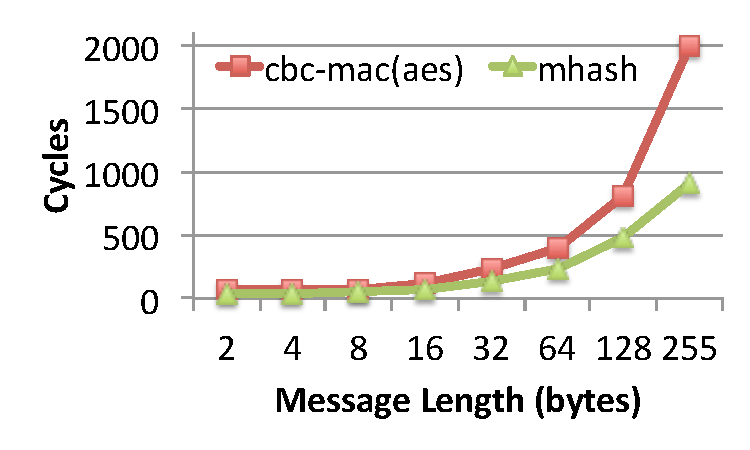
\includegraphics[width=.7\linewidth]{dcache/plots/hash.pdf}
\vspace{-10pt}
\footnotesize
\caption{
Cycles to hash messages of varying sizes using the 2-universal multilinear hash (mhash) and using the PRF cbc-mac(aes) using the Intel AES-NI instructions.
Lower is better; at lower values, cbc-mac(aes) is roughly twice as slow as mhash. }
\label{fig:hash}
\vspace{-10pt}
\end{figure}

Thus, the main reason to select a 2-universal function over a 
PRF is performance.  
Our design can use a hash function from either family.
Figure~\ref{fig:hash} compares the performance of hashing different message lengths
using the 2-universal multilinear hash function~\citep{lemire2013strongly}  (mhash)
and, as a PRF,
the CBC-MAC algorithm with hardware-accelerated AES
as the block cipher.
Because AES only creates a 128-bit hash value, we ran the algorithm twice with different keys to create a 256-bit output;
as a result, using CBC-MAC(aes) takes roughly twice as long as mhash.
In terms of the impact this has on lookup performance, 
mhash can outperform baseline Linux even for a single-component path,
whereas CBC-MAC(aes) is only faster than Linux with four path components.
We expect that, with hardware support for a 256-bit hash output, a PRF would be equally practical
for our purposes.

In order to realize the best performance, we use the mhash function in our experiments,
and carefully audit any code that calculates or compares signatures for potential side channels.
\fixmedp{Clear this fixme when done}
A more cautious implementation might favor a PRF to avoid any risk of overlooked side channels.
\end{comment}

%% \fixmedp{Educated speculation from here forward.  Revisit once we have numbers}
%% For a PRF, we used the CBC-MAC algorithm to create a signature, using AES
%% as the block cipher.  
%% Because AES only creates a 128-bit hash value, we ran the algorithm twice with different keys to create a 256-bit output.
%% In our experiments, hardware-accelerated AES instructions make the cbc-mac(aes)
%% fast enough to accelerate lookup by \fixmedp{XX\%} for the test in Figure~\ref{fig:by-version}.
%% The 
%% also improves lookup by \fixmedp{XX\%} in this test.
%% Because the improvements from a 2-universal hash are marginal,
%% we err on the side of caution and report only results with a PRF-based signature.


\paragraph{Probability of a signature collision.}
We selected a 240-bit signature, 
which is comparable to signature sizes used in data 
deduplication systems, ranging from 128--256 bits.  Deduplication designs commonly 
select a signature size that introduces a
risk of collisions substantially less than the risk of undetected ECC RAM 
errors~\citep{Debnath:2010:CSU:1855840.1855856, Srinivasan:2012:ILI:2208461.2208485, Quinlan:2002:VNA:645371.651321, Zhu:2008:ADB:1364813.1364831}.

We assume an adversary that is searching for collisions by brute force.
This adversary must lookup paths on the system,
such as by opening local files or querying paths on a web server.
Because our hash function is keyed with a random value and the output is 
hidden from the user,
the adversary cannot search for collisions except on the target system.
Thus, the adversary is limited by the rate of lookups on the system,
as well as the capacity of the target system to hold multiple signatures
in cache for comparison.

%Assuming an adversary is using brute force to find a collision,
We calculate the expected time 
at which the risk of a collision becomes non-negligible (i.e., higher than $2^{-128}$) 
%to find a collision 
%with a 240-bit hash value, and
%Suppose the adversary makes $t$ attempts to look up any paths in the directory cache, 
and model the risk of collision as follows.
First, $|H(X)|=2^{240}$ is
the number of possible signatures.
We  limit the cache to $n=2^{35}$ entries (i.e., assuming 10TB of dcache space in RAM and 320 bytes per entry),
with an LRU replacement policy.
We calculate the number of queries ($q$) after which the risk of a collision is 
higher than $P=2^{-128}$ as follows:
\begin{align*}
q \simeq ln(1 - p) * \frac{|H(x)|}{-n} \simeq ln(1-2^{-128}) * \frac{2^{240}}{-2^{35}} \simeq 2^{77}
\end{align*}
At a very generous 
lookup rate of 100 billion per second (current cores can
do roughly 3 million per second),
the expected time 
%in the brute force attack
at which the probability of a brute-force collision goes above $2^{-128}$
is 48 thousand years.

%% If one does a similar calculation with a completely unbounded 
%% dcache (i.e, each new signature is compared against all previous signatures),
%% the expected time drops to 8 years.
%% In such a worst case, the cache can be dropped and a new random signature key selected
%% after every 8 years of uptime, but with any reasonable bound on the cache size,
%% this should not be a concern.

%% and an uptime of 10 years, for $t \simeq 3.16 * 10^{19}$.
%% We assume an unbounded directory cache.
%% The probability of successfully causing any collision is:

%% \vspace{-0.15in}
%% \begin{align*}
%% P_{Adv}(t,H(X)) \simeq 1 - \epsilon^{-\frac{t^2}{2|H(X)|}}
%% \end{align*}
%% \vspace{-0.15in}

%% Thus, with 192 signature bits, the probability of a collision
%% is less than XXX, which is algorithmically negligible.

%% In order to less than a one in a billion \fixmedp{machines?}
%% the number of attempts by the adversary must be at least:

%% \vspace{-0.15in}
%% \begin{align*}
%% T_{Adv}({10}^{-9},2^{192}) \simeq \sqrtsign{\ln{(1-{10}^{-9})} \times -2 \times 2^{192}} \simeq 2^{81}
%% \end{align*}
%% \vspace{-0.15in}


%% In a system with 10-year uptime, assuming the directory cache is never shrinked, an adversary must perform at least ${10}^{17}$ lookups per second, to achieve one success in a billion manipulated systems. Such an adversary is computationally impossible to succeed in the real world.

%% \fixmedp{I'm confused.  We seem pretty far from $2^{-128}$.  Also, I'm not sure why we are talking about the number of systems.  Let's assume the number of systems is independent and focus on one system, since each has a different random key.}

\begin{comment}

\fixmedp{Chia-Che, please update these calculations.  What happens if we do things Michael's way?}
\fixmedp{once this is resolved, respond to D6}
\fixmedp{Add a note that this is an upper bound and why (just check that what is going on is clear after revision}

We consider two possible collision cases separately.
First, consider the case where two \dentries{} in the cache have a 
matching signature.
This type of collision could cause an application to access the wrong file,
and eventually retrieve wrong content or corrupt the file.
The probability of this type of collision is:
%
\begin{align*}
P_+(n,H(X)) = \frac{n(n-1)}{2} \times \frac{1}{|H(X)|} \simeq \frac{n^2}{2|H(X)|}
\end{align*}
%
where $n$ is the number of directory entries in the system, and $|H(X)|$ is
the number of possible signatures.  

The second type of collision happens if a user 
asks for a path that does not exist in the cache, which 
collides with an existing directory entry
with a different path.
This type of collision will cause the application to
assume existence of a nonexistent file and potentially corrupt other files.
The probability of this type of collision among $q$ queried paths is:

\vspace{-0.15in}
\begin{align*}
P_-(n,H(X),q) = 1 - (1 - \frac{n}{|H(X)|})^q \simeq 1 - \epsilon^{-q\frac{n}{|H(X)|}}
\end{align*}
\vspace{-0.15in}

We argue that the probability of both types of collision is negligible
when using a 192-bit universal hashing function to generate path signatures.
In our assumption, most systems will devote no more than 16GB of physical memory in directory cache, indicating that at most $\simeq 10^8$
\dentries{} will coexist at the same time.
A very busy system with a 10-year uptime, performing an average of 1000 lookup per second,
will query the directory cache for $3\times{10}^{11}$ times ($=q$).
%The number of directory entries is much smaller than
%the number of actual files and directories on storage because directory cache only keeps entries
%that are most recently accessed.
%has the longest possible history of queries.
Using a 192-bit signature, number of possible signatures is ${2}^{192}$ (=$|H(X)|$).
The probability of either collision can be calculated as follows:

\vspace{-0.15in}
\begin{align*}
P_+(10^8,{2}^{192}) \simeq \frac{{(10^8)}^2}{2\times{2}^{192}} \simeq {2}^{-139}
\end{align*}
\vspace{-0.28in}
\begin{align*}
P_-(10^8,{2}^{192},3\times{10}^{11}) \simeq 1 - \epsilon^{-3\times{10}^{11}\frac{10^8}{{2}^{192}}} \simeq {2}^{-128}
\end{align*}
\vspace{-0.15in}

In conclusion, with a directory cache no larger than 16GB, 192-bit signatures make the risk of collision 
negligible within $3\times{10}^{11}$ lookup operations,
or roughly every 10 years.
If a system decides to dedicate more physical memory than 16GB in directory cache,
longer signatures will have to be used,
or a shorter life span of the system must be assumed.
We can enforce this assumption and mitigate the risk of brute force attacks 
by changing the signature key,
and dropping or recalculating the signature for all dcache entries
after this threshold of lookups has been met.

\paragraph{Adversary Resistance.}



Because permission check only happens on the {\em slowpath}, signature collision will never cause security breach with benign users. However, many priviledged processes (e.g. Setuid-to-root programs, system services) in the system can be manipulated by a malicious user to exploit signature collision.
Fortunately, the strength of such an adversary is limited by the system latency, because it cannot perform an offline attack to the signature algorithm, but brute-forcely attempt for lookup in the system.

Assume a stronger adversary uses {\em Birthday Attack} to discover any pairs of paths that have signature collision. Suppose the adversary makes $t$ attempts to look up any paths in the directory cache, the probability of successfully causing any collision is:

\vspace{-0.15in}
\begin{align*}
P_{Adv}(t,H(X)) \simeq 1 - \epsilon^{-\frac{t^2}{2|H(X)|}}
\end{align*}
\vspace{-0.15in}

In other word, to achieve $10^{-9}$ success rate (one in a billion machines), the number of attempts by the adversary must be at least:

\vspace{-0.15in}
\begin{align*}
T_{Adv}({10}^{-9},2^{192}) \simeq \sqrtsign{\ln{(1-{10}^{-9})} \times -2 \times 2^{192}} \simeq 2^{81}
\end{align*}
\vspace{-0.15in}

In a system with 10-year uptime, assuming the directory cache is never shrinked, an adversary must perform at least ${10}^{17}$ lookups per second, to achieve one success in a billion manipulated systems. Such an adversary is computationally impossible to succeed in the real world.
\end{comment}



%The probability of either type of collision is lower than $2^{-128}$,
%which is algorithmically negligible.
%Because mean-time-to-failure (MTTF) of most hard drives ranges from $10^6$ to $1.5\times10^6$ hours~\citep{schroeder07mttf},
%any directory collisions will be indistinguishable from a disk sector 
%failure that corrupts directory metadata.
%\fixmedp{Let's consider dropping the first case for space here.}

%it is guaranteed that any systems will have to restart to recover from disk \fixmedp{sector?} failures before collision happens in the directory cache.

%At high probability, the collision will never appear in the history of queries
%before the system is restarted.

%% The only possible attack using signature collision is to maintain
%% an oracle of all queried paths for brute-force attack across system restart.
%% To defend this attack, we use a randomly generated seed to randomize
%% the hashing function every time the system starts. 

%% In our threat model, we are not defending any offline birthday attack
%% that deliberately queries two paths or creates two files that are known to
%% have colliding signatures.
%% These attacks is not a threat for us because they cannot bypass
%% permission check while accessing the files.
%% In most cases, an adversary that uses birthday attack can only corrupt
%% a file that it already owns the access right.
%% The worst scenarios is that the adversary may trick a seteuid-to-root
%% program to enter a directory which it does not have privilege to.  



\begin{comment}
A good design of caching systems requires a fully optimized lookup method,
which uses the fastest way possible to
determine whether requested data exists in the cache.
Efficiency of the lookup method is especially essential and dominating the
overall lookup performance when
the caching system has a significantly high hit rate.
In the directory cache, a high hit rate can be expected in file systems with temporal locality in file access pattern, low memory pressure
and infrequent metadata relocation.
We predict that these characteristics can be found in majority of systems,
because applications are inclined to access files repeatedly,
and enough spared memory is often available.
These systems will certainly benefit from any improvement on the efficiency of
directory cache lookup.

The directory cache in current Linux kernel uses component-based lookup.
To search for a requested file, the lookup routine will scan and delimit 
every component in path of the file,
and iterate through chained entries in correspondent hash buckets as many times
as the number of components.
The latency of directory cache lookup will grow linearly as longer and deeper
paths are queried.
Despite many efforts have been made in Linux kernel, directory cache lookup
is still one expensive cost to pay in many file system operations. 

We present the design of a significantly faster directory cache lookup
for Linux \linuxver{} kernel.
The lookup method can maximize the speed of searching
a directory entry for a target file which is previously accessed and 
has its metadata cached in memory.


The basic design of our lookup method is simple:
To search the directory entry for a requested file,
instead of breaking the path of file into components and iterates hash buckets repeatedly,
we use a hashing function that maps the whole canonical path of the file
into the index of hash bucket,
and directly look up the directory entry that stores the metadata of the last component.
If the directory entry is found, it is returned immediately to caller routine
for file system operations.
If the directory entry is not found, it is a case of cache miss.
When a cache miss happens, VFS asks file system drivers to locate
and retrieve metadata from the storage.
\end{comment}

%% To deal with cache misses,
%% our solution keeps the original component-based lookup method of Linux kernel,
%% as a slow path to fall back when our lookup method fails searching the
%% directory entry.
%% When a cache miss happen, even if the directory entry for the requested file
%% does not exists in the cache, the parent directories of the file may have been
%% accessed and have their directory entries created.
%% Using component-based lookup as slow path can recollect all created parent
%% directory entries, and request file system drivers to retrieve metadata of the rest
%% of parent directories and the files to cache.
%% Because the file system driver interface of Linux kernel is designed to look
%% up metadata by the parent directory and a file name,
%% using component-based lookup can keep file system drivers unchanged,
%% which can largely alleviate the pain of porting third-party file system driver
%% codes to the new directory cache design.

%% Another reason of using component-based lookup as slow path is to
%% calculate user access right against the target file.
%% To allow an user to access a file, the user requires not only the privileges
%% of file operations,
%% but also permission to enter every parent directory of the file.
%% The easiest way of calculating the permission is to resolve the access right
%% at each parent directory,
%% while looking up entries by each component of the path.
%% Once the permission of a directory or a file is calculated in the slow path,
%% we cache the permission in directory entry
%% and reuse it to determine the access right at next time when
%% the directory entry is looked up in the fast path.
 
%% The permission cached in directory entries is bound to the user credential
%% of process who performs the slow path.
%% If a different user credential look up a directory entry by the fast path,
%% it cannot be guaranteed to have permission to access the file.
%% For example, user {\tt A} and {\tt B} accesses the file {\tt /home/foo/bar},
%% but only user {\tt A} has the permission to entry the directory {\tt /home/foo}.
%% If user {\tt A} has accessed the file first, the kernel will create the directory
%% entry of {\tt /home/foo/bar}, which can be directly looked up in the fast path
%% by user {\tt B}.
%% In these cases of {\bf permission cache miss}, we must
%% force directory cache lookup to fall back to the slow path, in order to calculate
%% the access right for the new user credential.




%% The design of constructing a faster lookup method upon a slower one
%% is comparable to the concept of {\bf TLB (translation lookaside buffer)}.
%% TLB is a hardware optimization of multiple-level page tables traversal
%% in MMU to
%% translate virtual memory addresses into physical pages.
%% By falling back to page table traversal, TLB can recover from incoherence
%% without a sophisticated synchronization and update scheme.
%% The operating system only needs to flush the TLB timely whenever incoherence
%% is suspected or the page table needs to be updated.
%% Similarly, our fast lookup method for file system directory cache works without
%% any logic to update or to sync up directory entries, but simply fall backs to
%% slower component-based lookup to reassure coherence.

%% \paragraph{Expected Speed-up of Lookup Time}
%% Based on expected hit rate, we can predict the average lookup time
%% in directory cache
%% before and after applying the fast path:

%% \vspace{-0.22in}
%% \begin{flalign*}
%% & {Lookup\;time}_{original} = {Time}_{slow\;path} + {Time}_{storage\;lookup} \\
%% & \times (1 - (Hit\;rate))\\
%% & {Lookup\;time}_{optimized} = {Time}_{fast\;path} \times (Hit\;rate) \\
%% & + ({Time}_{slow\;path} + {Time}_{storage\;lookup}) \times (1 - (Hit\;rate))
%% \end{flalign*}
%% \vspace{-0.22in}

%% From the expected lookup times, we can calculate the improvement of performance as follows:

%% \vspace{-0.22in}
%% \begin{flalign*}
%% & {Speed\;up} = \frac{({Time}_{slow\;path} - {Time}_{fast\;path}) \times (Hit\;rate)}{{Lookup\;time}_{original}}
%% \end{flalign*}
%% \vspace{-0.22in}

\section{Generalizing the Fast Path}
\label{sec:generalize}

Thus far, we have explained our fast path optimization using the relatively straightforward
case of canonical path names.  
This section explains how these optimizations integrate with Linux's
advanced security modules,
%, such as SELinux~\citep{selinux} and AppArmor~\citep{apparmor},
as well as how we 
address a number of edge cases in Unix path semantics,
%which must be implemented correctly, 
such as mount options, mount aliases, and symbolic links.  
%Linux also includes a number of  which must work correctly with any VFS-level optimizations.
%This section explains how we address these challenges.

\subsection{Generalizing Credentials}
\label{sec:dcache:cred}
\label{sec:dcache:selinux}

%Two key requirements of our dcache optimizations are that they must be general
%and that space overheads for extra metadata must be minimized.
Linux includes an extensible security
module framework (LSMs~\citep{wright+lsm}), upon which SELinux~\citep{selinux}, AppArmor~\citep{apparmor}, and others are built.
An LSM can override the implementation of search permission checks,
checking customized attributes of the directory hierarchy or
process.
Thus, our dcache optimizations must still work correctly even when an LSM overrides the default access control rules.
%the default definition of 
%we need a general mechanism to encapsulate all possible credentials of a process with minimal 
%space overhead in the \dentries{}.

Our approach leverages the {\tt cred} structure in Linux, which is designed to store 
the credentials of a 
process ({\tt task\_struct}), and has several useful properties.
First, a {\tt cred} struct is comprehensive, including all variables that influence default permissions,
and including an opaque {\tt security} pointer for an LSM to store metadata.
Second, a {\tt cred} is copy-on-write (COW), so when a process changes its credentials, such as 
by executing a {\tt setuid} binary or changing roles in SELinux, 
the {\tt cred} is copied.  We manually checked 
that AppArmor and SELinux respect the COW conventions for changes to private metadata.
Moreover, a {\tt cred} can be shared by processes in common cases, such as a shell script forking children with the same credentials.
Thus, the {\tt cred} structure meets most of our needs, with a few changes, which we explain below.

%\fixmedp{Clarify per-process is shared with common cred}

%As explained in Section~\ref{sec:dcache:prefixcheck}, 
We store cached prefix checks (\S\ref{sec:dcache:prefixcheck}) in each  {\tt cred} structure,
coupling prefix check results with immutable credentials.
New {\tt cred} structures are initialized with an empty PCC.
When more processes share the PCC, they can further reduce the number of slowpath lookups.


%% describe two designs of prefix check caching:
%% one is using a prefix check cache in each \dentry{},
%% and one is using a \dentry{} lookup table in each {\tt cred} structure.
%% The former uses a 63-bit integer, called the credential identifier (CID), as a layer of indirection to {\tt cred},
%% while the latter simply places a pointer in {\tt cred} to reference the DLT.
%% Using CID, we must handle the very infrequent case of CID wrap-around.
%% Using DLT, we can avoid handling CID wrap-around, and have better space efficiency as explained in section~\ref{sec:dcache:prefixcheck}.

%to minimize the complexity of freeing and reallocating the {\tt cred} structure itself.
%A simple alternative would have been to simply store the kernel virtual address of the {\tt cred} in 
%various \dentry{} prefix caches, but these caches would have to be cleared before the {\tt cred} is 
%freed, lest a recycled {\tt cred} obtain access to a stale prefix.
%Rather than incur this bookkeeping cost, we simply assign a unique CID integer value to 
%Each time a {\tt cred} is allocated and reused, a new CID is assigned to the cred.
%The CID approach allows stale CID's to safely persist in a prefix cache until they are evicted by LRU,
%and does not complicate freeing a {\tt cred}.

%Using CID, we must handle the very infrequent case of CID wrap-around
%by simply resetting 
%the CID of all active {\tt cred} and clearing all prefix caches.
%We note that, even if an extremely efficient machine changed credentials one trillion 
%times per second
%(cf.\ current cores process at most 4 billion instructions/second),
%a wrap-around would occur once every 106 days. 
%We believe this is acceptable:
%most end-user machines reboot for kernel patches more frequently than this, 
%and even highly-available systems can afford to clear the prefix check cache 
%(not the entire dcache) a few times a year in exchange for the demonstrated benefits.



% reuse
%% The key challenge of implementing permission caching is
%% to identify security credentials within cached permission records in each directory entry.
%% If the access rights of a process are changed, such as updating user/group ID by calling system call {\tt setuid} and {\tt setgid}, or applying new SELinux labels or AppArmor rules,
%% the previous cached permissions should not be
%% reused in the lookup routine if it can cause privilege escalation.

%% Our solution uses the {\tt cred} structure defined in Linux kernel to identify different security credentials.
%% The {\tt cred} structure is a kernel structure referenced by {\tt task\_struct},
%% to store all real/effective user/group IDs, capability, security labels and security records of processes.
%% The {\tt cred} structure can be shared by related threads and processes,
%% so child processes or other threads will not need be forced to recalculate permissions
%% if the directory entry is looked up once by the parent process.
%% Another reason of identifying by {\tt cred} structures
%% is that the {\tt cred} structure in each {\tt task\_struct} is always
%% recreated if the access rights are changed.

%% In order to identify cached permission by {\tt cred} structures,
%% our solution assigns a credential ID to every {\tt cred} structure allocated in the kernel.
%% The credential IDs are allocated incrementally, so they will not be reused soon
%% when {\tt cred} structures are destroyed.
%% Whenever the permission is recalculated, the credential ID of the {\tt cred} structure referenced by the current {\tt task\_struct},
%% will be assigned to the permission cache in the directory entry.
%% The credential ID in permission cache is later used to determine whether the permission can be reused by calling processes.

%Either placing CID or DLT in the {\tt cred} structure,
%it is always beneficial to share cached prefix check with more processes that share the same critical credentials.

One challenge is that Linux often 
allocates new {\tt cred} structures {\em even when credentials do not change}.
The underlying issue is that COW behavior is not implemented in the page tables, 
but rather by convention in code that {\em might} modify the {\tt cred}.
In many cases, such as in {\tt exec}, it is simpler to just allocate another {\tt cred} in advance,
rather than determine whether the credentials will be changed.
This liberal allocation of new {\tt cred}s 
creates a problem for reusing prefix cache entries across child processes 
with the same credentials.
To mitigate this problem, we wait until a new {\tt cred}
is applied to a process ({\tt commit\_creds()}).
If the contents of the {\tt cred} did not change, the old {\tt cred} and PCC is reused and shared.

%Only when Linux Security Module (LSM) specify that the new process has a different credentials,
%CID or DLT will be allocated when
%we defer allocation of the 
%CID or DLT
%the {\tt cred} is actually applied to the process ({\tt commit\_creds()}),
%and only allocate a new CID if the contents have changed.

%\fixmedp{Maybe cut if not implemented?}
%% In order to safely reuse {\tt cred} structures with LSMs,
%% we added a return parameter to the LSM credential initialization hook 
%% to communicate whether the credential changed with respect to prefix checking.
%% This optimization is our only modification to the LSM API and is optional;
%% without this change, we can disable {\tt cred} structure reuse with a LSM.

%%%  is a helpful optimization; without this LSM ch
%%% \fixmedp{How does the LSM determine if cred are equal?  Some function?  I just cut for now}
%%% \fixmetsai{Answered below}
%%% We rely on LSM to specify whether a credential change is relevant to file system traversal.
%%% For example, upon updating application profiles using {\em AppArmor},
%%% or altering {\tt search} permission on directory objects using {\em SELinux},
%%% or simply setting user IDs
%%% or adding {\tt CAP\_DAC\_OVERRIDE} capability to a process,
%%% the LSMs or VFS can mark the PCC in the new {\tt cred} as stale, and force allocating a new PCC at {\tt commit\_creds()}.

%dp: Not impl, not that interesting
%% To further improve reuse of cached prefix check,
%% we track the most recently used {\tt cred} structures in a hash table, keyed by the content of the structure.
%% %% dp: Ok
%% %\fixmetsai{I believe it should be "most recently used cred" because we are exploiting the temporal locality}
%% If a newly allocated {\tt cred} structure matches a recently used {\tt cred},
%% the old {\tt cred} and PCC are reused.
%% %has a matching credential, %according to the LSM,
%% %we can then reuse the CID or DLT.
%% %we then check the hash table for 
%% %a reusable CID.
%% This captures the case where identical credentials appear independently, such
%% as one user with two ssh connections to the system.
%Our solution maintains a credential cache with limited size,
%which can track credential IDs of most recently referenced {\tt cred} structures.
%For each {\tt cred} structure, a signature is generated based on
%all access rights related and can be used to match with the credential cache.
%\end{comment}

%% We predict that permission caching with credential identification is effective
%% on limiting the penalty of lookup performance
%% for recalculating permissions.
%% We observe that temporal locality of directory cache lookup
%% is often delimited among the files accessed by
%% related application processes,
%% which mostly share security credentials.
%% As a result, the performance loss caused by permission cache miss is often trivial
%% in most systems. 

Our {\tt cred} approach memoizes complex and potentially arbitrary
permission evaluation functions
of different LSMs. %, with minimal memory overhead.
%% SOSP Space
%% In contrast, the recent DLFS file system~\citep{lensing13dlfs} minimized disk seeks
%% to lookup a file that is not in the dcache (i.e., optimizing the miss path for prefix checking).
%% DLFS stored the parent permissions as a closed-form expression on disk.  Not only does this require
%% substantially more space, but it doesn't easily generalize to LSMs.


\subsection{Non-Canonical Paths and Symbolic Links}

Our optimized hash table is keyed
by full path.  However, a user may specify variations of a path, such as {\tt /\fnone{}/\fntwo{}/./\fnthree{}}
for {\tt /\fnone{}/\fntwo{}/\fnthree{}}.
Simple variations are easily canonicalized in the course of hashing.

A more complex case is where, if {\tt /\fnone{}/\lnone{}} is a symbolic link,
the path {\tt /\fnone{}/\lnone{}/../\fntwo{}} could map to a path other than {\tt /\fnone{}/\fntwo{}}.
Similarly, if the user doesn't have permission to search {\tt /\fnone{}/\fnthree{}}, 
a lookup of {\tt /\fnone{}/\fnthree{}/../\fntwo{}} should fail even if user has permission to search
{\tt /\fnone{}/\fntwo{}}.
In order to maintain bug-for-bug compatibility with Linux,
our prototype issues an additional fastpath lookup at each dot-dot to check
permissions. % and to handle symbolic links (discussed more below).
Maintaining Unix semantics introduces overhead for non-canonical paths.

We see significantly higher performance by using
%We suggest that users should also be given the opportunity to reduce these overheads by using 
Plan 9's {\em lexical}
path semantics~\citep{pike00lexical}.  %, on an opt-in basis.
Plan 9 minimized network file system lookups by pre-processing
paths such as {\tt /\fnone{}/\lnone{}/../\fntwo{}} to {\tt /\fnone{}/\fntwo{}}.
We note that Plan 9 does component-at-a-time lookup, but does not have a directory cache.
%% dp: SOSP Space
%Plan 9 eschews symbolic links and Unix compatibility for paths at several points.

%We expect such a behavior would be similar to the {\tt noatime} mount option, 
%which disables a particularly expensive and rarely used 
%Unix behavior\citep{atime-sux}, except when needed by a legacy application.

\paragraph{Symbolic Links.}  We resolve symbolic links on our lookup fastpath
by creating \dentry{} aliases for symbolic links.
For instance, if the path {\tt /\fnone{}/\lnone{}} is an alias to {\tt /\fnone{}/\fntwo{}},
our kernel will create dentries that redirect {\tt /\fnone{}/\lnone{}/\fnthree{}} to {\tt /\fnone{}/\fntwo{}/\fnthree{}}.
In other words, symbolic links are treated as a special directory type, and can create children,
caching the translation.

Symbolic link dentries store the 240-bit signatures that represent the target path.
The PCC is separately checked for the target \dentry{}.
If a symbolic link changes, we must invalidate all descendant aliases,
similar the invalidation for a directory {\tt rename}.
This redirection seamlessly handles the cases where
permission changes happen on the translated path,
or the referenced \dentries{} are removed to reclaim space.


%% Because the directory structure may change at any moment, we choose not to
%% store any pointers to the referenced \dentries{} in the aliases.
%% Instead, we store 
%% during lookup,
%% use a separate fastpath walk to search for the \dentries{}.  

%\fixmedp{Add a figure with the symlink dentry}

%% Tao tested these shells, none do canonicalization:
%% busybox
%% csh
%% dash
%% fish
%% ksh93
%% mksh
%% pdksh
%% rc
%% tcsh
%% zsh

%In order to keep these translations coherent, symbolic link aliases must also store pointers 
%to the symbolic links that led to them and the target signature.  These links and signatures are validated 
%at lookup time.  In order to minimize this space overhead, we currently bound the symbolic link depth to 4
%and require deeper sets of links to follow the slow path.
%We expect common use cases to only redirect a path once or twice.

%%% A symbolic link can be resolved in the fast path
%%% if the target file itself is the symbolic link.
%%% However, a symbolic link may exist at one of the parent directories of the target file,
%%% and the file becomes an alias of another file
%%% under the directory where the symbolic link points to.
%%% For example, the path {\tt /home/foo/bar} will be an alias of {\tt /other/bar},
%%% if {\tt /home/foo} is a symbolic link that points to {\tt /other}.  
%%% When this case happens, the alias of target file cannot be looked up
%%% in the fast path,
%%% because no directory entry is ever created for the alias in the slow path.
%%% Although the alias can still be looked up in the slow path,
%%% accessing the file cannot benefit from the speed up of our lookup method.
%%% In many systems, resolving symbolic links can be a frequent operation
%%% if a symbolic link is created as a shortcut to
%%% some of the most frequently accessed files, such as personal folders or
%%% important system files and binaries.
%%% For example, the GNU C compiler {\tt /usr/bin/gcc} is often created as a symbolic
%%% link to the actual binary of latest release (e.g. {\tt /usr/bin/gcc-4.6}),
%%% to keep flexibility of switching between binary releases.

%%% \fixmetsai{nail down the detail of symbolic links.}


\begin{comment}

Plan 9 introduced the idea of 
optimization through lexical path semantics~\citep{pike00lexical}.  Specifically, in Unix and Linux,
the path {\tt /home/alice/../bob} could map to a path other than {\tt /home/bob}
if {\tt /home/alice} is a symbolic link.  In Plan 9, this path can be pre-processed
to {\tt /home/bob} before lookup, with the assistance of a per-process, lexical substitution table.

%The authors specifically recommend that Unix variants should experiment with lexical semantics;
This paper adapts this lexical canonicalization strategy, but
uses it to do a constant number of component lookups in the common case, as well as 
maintaining compatibility with Unix semantics and legacy applications.


%\fixmedp{Can someone figure out if this is actually part of POSIX?}
Our prototype does change an arguably silly behavior of the {\tt ..} path component.
Suppose Bob tries to open path {\tt /home/alice/../bob/foo.txt}.
If Bob doesn't have permission to search Alice's home directory, this lookup should 
fail even if Bob can open {\tt /home/bob/foo.txt}.  
Assuming that {\tt /home/alice} is not a symbolic link (a case we discuss below)\fixmedp{Revisit},
there is no particularly good reason not to optimize this path to {\tt /home/bob/foo.txt} 
as part of canonicalization, but rather this is an artifact of an implementation creeping 
into the interface.

Nonetheless, we could easily simulate this behavior by checking intermediate components at each {\tt ..}, albeit at some additional cost.
\end{comment}

%\fixmedp{Does this simple xor-ing scheme damage our analysis?  Seems to undermine universality.  Do we still do this in our implementation?  Also, the more I read this, the more this feels too far down in the weeds.  Commenting for now}
\begin{comment}
In our lookup method, the hashing function is called
as a one-time effort before searching the directory entry for any file.
In order to compute the hash value efficiently, we choose the hashing function
that requires no canonicalizing the paths beforehand.
We reuse the fast component hashing function {\tt $h_{simple}(C)$}
in currently Linux kernels to construct our hashing function:
 
\vspace{-0.22in}
\begin{flalign*}
& H(C_1/C_2/..../C_n) =\\
& h_{simple}(C_1) \oplus h_{simple}(C_2) \oplus ... \oplus h_{simple}(C_n)
\end{flalign*}
\vspace{-0.22in}
 
The hashing function is fast because {\tt $h_{simple}(C)$} is designed to be
much faster than other universal hashing functions.
The hashing function can be computed as the queried path is scanned,
even if the path is not canonical.
For example, when a {\bf dot-dot (..)} is scanned in the path, 
our hashing function can roll back the hashing result,
by XOR'ing with the hash value of last scanned component.
\end{comment}


\subsection{Mount Points}

Our fastpath handles several subtle edge cases introduced by mount points.
%The final challenge we faced in generalizing the {\em fastpath}
%was handling several edge cases in how mount points can affect lookup in subtle ways.

%\fixmedp{I am again confused.  Why wouldn't this just be rolled into the prefix check on the slowpath?}
\paragraph{Mount options.}  Mount options, such as read-only or nosuid,
can influence file access permission checks.
The Linux \dcache{} generally notices mount points as part of the hierarchical file system walk,
and checks for permission-relevant mount flags inline.
Once this top-down walk is eliminated, we need to be able to identify the current mount point for any given \dentry{}.
We currently add a pointer to each \dentry{}, although more space efficient options are possible. 
%\fixmedp{Make a global table if time?  Revisit after solving namespace issues}


%% Many file system routines require not only directory entry of the file to access,
%% but also looking up the record of mount point for the file.
%% For example, while writing to a file, the kernel needs to check certain
%% attributes of the mount point,
%% such as whether it is mounted as read-only file system.
%% Sometimes, file system drivers maintains global states of file system
%% in the mount point, which cannot be referenced directly from directory entries
%% or inodes.

%\fixmedp{I'm not sure I get the relevance of crossing mount points.  Revive this text if I missed something important.}
%% The original design of directory cache lookup
%% in Linux kernel
%% keep track of mount points along with directory entries
%% during component-based lookup.
%% However, if a directory entry is directly looked up,
%% the kernel cannot tell whether the path has crossed any mount point
%% from the root to the target directory entry.
%% Fortunately, directory entries stay under the same mount point
%% in most occasions.
%% Only renaming across mount points will cause directory entries to move from
%% one mount point to another.
%% We simply maintain a pointer in each directory entry to
%% reference back to its mount point.

%\fixmedp{I need some help understanding this.  I'd like to discuss before I edit this one.}

\paragraph{Mount Aliases.}
Some pseudo file systems, such as {\tt proc}, {\tt dev}, and {\tt sysfs},
can have the same {\em instance} mounted at multiple places.
This feature is used by {\tt chroot} environments and to 
move these file systems during boot.
A {\tt bind} mount can also create a mount alias.
%Mount aliases can also creating by mounting a 

In our system, a \dentry{} only stores one signature and can only be in the direct lookup hash table
by one path at a time.  
Our current design simply picks the most recent to optimize---favoring locality.
If a slowpath walk notices that the matching \dentry{} (by path) has a different signature,
is under an aliased mount, and is already in the DLHT, the slowpath will replace the signature,
increment the \dentry{} version count, and
update the pointer to the \dentry{}'s mount point.
The version count increment is needed in case the aliased paths
have different prefix check results.
%As the only caveat, we must invalidate PCC for the \dentry{} because permission can be different for another path. 
This approach ensures correctness in all cases, and good performance on the most recently used path for any mount-aliased \dentry{}.

\begin{comment}
The challenge is that the same \dentry{}
under different mount aliases can be accessed by different canonical path.
% to make drivers of these file systems able to dynamically append an remove nodes,
%even at early stages of boot. \fixmetsai{Please read this. I believe this is the reason why they do so.}
Our system must handle the case where a lookup creates and hashes a \dentry{}
under one mount and then searches for the same \dentry{} under a second mount using a different path.
We address this problem by creating \dentry{} aliases when searching under the second mount.
Like \dentries{}, these \dentry{} aliases also have a pointer that points to the mounts they are rooted, which may have different mount options as their mount aliases. 
It is similar to the approach of supporting symbolic links.
\end{comment}

%We address this problem by only allowing fastpath lookups to succeed on the most
%recently created mount alias.  When a second mount point is created, all active 
%dentries are moved to the newer mount point, except for {\tt chroot} cases.
%Fastpath lookups will fail under the old mount point,
%but redirect to the alias on the component-at-a-time, slowpath lookups.

%We initially permitted duplicate dentries to be created as aliases, 
%but found this not terribly useful, as the majority of accesses used the more recent mount alias,
%and the complexity overhead of keeping alias dentries coherent was substantial.


%% Sometimes multiple mount points may be sharing the same directory entries.
%% Sharing mount points is not an issue in component-based lookup
%% because the hierarchy of directory entries still remain the same under the
%% mount points.
%% However, according to the location of mount points,
%% a directory entry that is shared among mount points can have multiple
%% aliases of paths.
%% Using our lookup method it can only find the directory entry by one of the aliases,
%% but quering any of other aliases with cause a cache miss.

%% Two reasons can cause multiple mount points to share directory entries.
%% The first reason is to bind a mount point as an alias of another.
%% When two mount points are bound, any file operations made on one of the mount points
%% will happen on the other mount point immediately.
%% The second reason is that some special file systems, such as {\tt Proc}, {\tt Dev}, {\tt SysFS} file systems,
%% maintains global file system states shared among all mount points of the same type.

%% We combined two solutions to track directory entries shared across mount points.
%% The first solution is to hash the directory entry based on
%% the alias that is most recently accessed.
%% The penalty of this solution is that when other aliases of the directory entry
%% is requested, the kernel must fall back to the slow path for lookup.
%% The second solution is to clone the whole tree of directory entries for different
%% mount points, so each directory entry will be linked with exactly one alias.
%% Cloning directory entries at mount point aliases
%% can make lookup by the fast path possible for all aliases,
%% but requires updating all aliased directory entries in many file system operations such as creation, renaming or update metadata.
%% We pick the solutions based on the characteristics of file systems.
%% For example, a file system that constantly creates global visible directory entries,
%% mostly special files system,
%% will not clone directory entries at mount point aliases.  

\paragraph{Mount Namespaces.} Mount namespaces in Linux allow processes
to create private mount points, including {\tt chroot} environments, 
that are only visible to the process and its descendants.
When a process creates a new mount namespace, it also allocates a new, namespace-private direct lookup hash table.
The slowpath always incorporates any mount redirection, and any new signature-to-\dentry{} mappings will be correct
within the namespace.
Thus, the same path (and signature) inside a namespace will map to a different \dentry{} than outside of the namespace.
Similarly, the prefix check cache (PCC) will always be private within the namespace.

As with mount aliases, we only allow a \dentry{} to exist on one direct lookup hash table at a time.
This favors locality, and makes the invalidation task tractable when a renamed directory is shared across many namespaces.
The invalidation code used for directory tree modifications simply evicts each child \dentry{} from whatever
DLHT it is currently stored in.
%; this invalidation only requires a reference to the \dentry{} because the hash bucket list pointers are embedded
%in the \dentry{} structure.  

%% SOSP SPace
%Our current design is the product of several iterations; the current structure cleanly handles 
%each of these tricky cases, and maintains good performance in the common case.

\paragraph{Network File Systems.} Our prototype does not support 
direct lookup on network file systems, such as NFS versions 2 and 3~\citep{sandberg85nfs}.
In order to implement close-to-open consistency on a stateless protocol, 
the client must revalidate all path components at the server---effectively forcing 
a cache miss and nullifying any benefit to the hit path.
We expect these optimizations could benefit
a stateful protocol with callbacks on directory modification, such as AFS~\citep{howard88} or NFS 4.1~\citep{rfc5661}.


%%  (and {\tt cred}/prefix check cache).

%% \fixmedp{Chia-Che, check (and implement?).  I don't think a private CI}
%% The {\tt chroot} case is handled easily: each process stores a hash of its root path, and this is simply overridden.
%% Other mount points must be 

%% If a process has its own mount namespace, using the same canonical path it should find a different \dentry{} from other processes that are outside the namespace.
%% We seemlessly address the problem by forcing the process to create a new {\tt cred} structure and allocate a new CID or DLT.
%% With different CID or DLT, processes can see different view of file system on fastpath.  
%We do not currently support mount namespaces on the lookup fastpath,
%and non-default namespaces must take the lookup slowpath.
%We expect that the fastpath can be extended to mount namespaces 
%with process-local, lexical substitution tables, similar to Plan 9~\citep{pike00lexical}.


%%% Unlike other mount points, while mounting a file system in a mount namespace,
%%% the kernel cannot disconnect the directory entries of
%%% files and subdirectories under the directory where the mount point is created.
%%% The existing directory entries must remain visible to the rest of system,
%%% but processes in the mount namespace should be able to access files or directories under their private mount points.

%%% \fixmetsai{nail the detail of mount namespace}

%\fixmedp{I don't think the fastpath actually affects openat.  We can discuss if you disagree, but I'm commenting this.}
\begin{comment}
\paragraph{Atomic File Operations.} 
For many file system operations, recent Linux kernels provide a
set of system calls that perform the same operations, with atomicity guarantee.
For example, different from {\tt open},
the system call {\tt openat} accepts the descriptor of an opened file
as the root of directory cache lookup.
When {\tt openat} is used for opening an file,
the kernel can securely looks up the target directory entry,
with no interference from any concurrent renaming of its parent directories.  
These kinds of system calls are mainly designed for
defending {\bf time-to-check-to-time-to-use (TOCTOU) attacks}.

To preserve the security property of atomic file operations,
we force our lookup method to fall back to the slow path whenever
the lookup routine is called by one of these atomic system calls.
Because the slow path has no difference from the original lookup routine
of the Linux kernels, it maintains the same property of atomicity.
\end{comment}



%\subsection{Summary}
%
%This section demonstrates how our directory cache optimizations
%can support the wide range of features Linux has built
%upon the directory cache, including namespaces, enhanced security modules, and symbolic links.
%Our prototype focuses on Linux, which has arguably the most features intertwined with its directory cache,
%but we believe these optimizations would work in other systems, with modest 
%porting effort.
%
%Our design has the following requirements, which we expect would be met by any 
%POSIX-compliant directory cache.
%First, POSIX permission semantics require directory access checks on the path from
%the current root or working directory to the file (i.e., prefix checking);
%our implementation inherits Linux's invariant that any cached directory's parents are in the cache,
%but any design that can implement prefix checking should suffice.
%Second, we require that, if a directory's permissions change, there is a programmatic way to find all
%descendants in the cache (\S\ref{sec:dcache:rename}).
%Our implementation integrates with optimistic synchronization 
%in the Linux dcache for good performance and consistency, but 
%this design could integrate with any reasonable synchronization scheme, such as
%FreeBSD's reader/writer locks.  
%%% SOSP Space
%%We assume there is sufficient synchronization
%%in the kernel slowpath to prevent inconsistency during cache invalidation,
%%such as using a lock to ensure the atomicity of a directory rename.
%Finally, we leverage the fact that Linux has an immutable credentials structure (\S\ref{sec:dcache:cred});
%adapting to mutable or less consolidated credentials would require extra effort.
%

\section{Improving the Hit Rate}
\label{sec:readdir}

The previous sections explain how changes to the structure of the dcache
can lower the average hit latency, through algorithmic improvements.
This section identifies several simple changes that can improve the hit rate.
In the case of a dcache miss, the low-level file system is called to service the system call.
At best, the on-disk metadata format is still in the page cache, but must be translated
to a generic format; at worst, the request blocks on disk I/O.
%In each case, we demonstrate that the additional bookkeeping in the dcache is minimal.
Although not every application heavily exercises these cases with unusually low hit rates,
the evaluation shows several widely-used applications that substantially benefit 
from these optimizations.

%% This section discusses some typical cases in the directory cache of Linux kernels which
%% causes cache misses that are actually avoidable.
%% Based on our case study, these cases of unneeded cache miss
%% are not caused by implementation mistakes,
%% but false obedience to important design principles of caching systems.
%% We observe that these problems are not specific to Linux kernels,
%% but existing in many UNIX operating system kernels.

\subsection{Caching Directory Completeness}

Although the Linux dcache tracks the hierarchical structure of directories, 
it has no notion of whether a directory's contents are completely or partially in the cache.
Suppose Alice creates a new directory {\tt \fnone{}} on a local file system; 
if her next system call attempts to create
file {\tt \fnone{}/\fntwo{}}, the dcache will miss on this lookup and ask the low-level file system if {\tt \fnone{}/\fntwo{}} exists.  
This overhead can be avoided if the VFS tracks that
all directory contents are in the cache.
%This subsection observes a missed opportunity in not tracking %such obvious cases 
%that all 

A second example is {\tt readdir}, which lists the files in a directory,
along with 
their \inode{} number
and their types, such as a regular file, 
character device, directory, or symbolic link.
%Aside from creation of a new directory, the most common way to obtain a complete
%directory listing is through the VFS {\tt readdir} operation.
In the current VFS {\tt readdir} operation, 
the low-level file system is always called, {\em even if the entire directory
is in cache}.
%Readdir returns a listing of the files, both 
For directories too large to list in the user-supplied buffer,
{\tt readdir} may be called multiple times, storing an offset into the directory.
To construct this listing,
the low-level file system must 
reparse and translate the on-disk format,
and may need to read the metadata block from disk into the buffer cache.
As a result,
{\tt readdir} is generally an expensive file system operation,
especially for large directories. % with plenty of files.

%The {\tt readdir} operation is used to implement system calls such as 
%{\tt getdents}, which are called by the c 
%Directory listing ({\tt readdir}) is a frequently used operation implemented
%by file system drivers.
%The operation is often made by system calls {\tt getdents} or {\tt getdents64},
%which are called by the function {\tt readdir} in GNU Library C.


%% We suggest that cost of {\tt readdir} can be reduced by
%% avoiding requesting the file system driver repeatedly to list the same directories.
%% Because most file system drivers implement {\tt readdir} in a stateless way,
%% they must read all related blocks from the disk to construct the result.
%% The cost of {\tt readdir} is primarily dominated by disk IO for
%% reading data blocks and metadata blocks,
%% and interpretion of raw data to retrieve file names, types and inode numbers.

%% File system drivers may individually improve cost of {\tt readdir}
%% by either caching or changing placement of metadata.
%% For example, page cache is general useful in file system drivers
%% to buffer disk IO for retreiving metadata.
%% If related blocks for constructing a directory list is still buffered in memory since the last query,
%% the file system driver does not need to read from the disk again.
%% However, using page cache, the file system driver stil have to
%% interpret raw data from the cached pages
%% to get metadata needed for constructing the {\tt readdir} results.
%% File systems such as DLFS choose to internally cache most recent results of {\tt readdir},
%% so the results can be directly returned when the same directory is listed again.
%% These file system drivers can only maintain very limited size of result caching,
%% because memory management for controlling cache size is out of scope for
%% the implementation of file system drivers.
%% For instance, DLFS can cache only up to one result for each process,
%% which is replaced at the next {\tt readdir}.

We observe that repeatedly listing a directory is a common behavior
in file systems.
For example,
a user or a shell script may repeatedly run the {\tt ls} command
in a directory.
%If {\tt readdir} is called by an application who is confident that the
%directory list will stay static,
%it may avoid repeatedly listing directory by caching the {\tt readdir} results itself.
%However, 
Some applications coordinate state through directory contents,
requiring frequent and repeated directory listings.
For example, {\tt maildir} is a popular email back-end storage format~\citep{maildir},
yielding better performance scalability than the older {\tt mbox} format.
% way for IMAP and POP3 email server to store email message.
Maildir stores each inbox or subfolder as a directory,
and each individual message is a file within the directory.
File names encode attributes including  flags and read/unread status.
%For each mailbox or subfolder that an IMAP server stores in maildir format,
%it maintains several directories where it stores each received mail as a file,
%with file name as a tuple of a unique identifier, the email format version,
%and flags for the mail.
If a message changes state, such as through deletion or being marked as read,
% mail is marked with certain flags,
the IMAP server server will rename or unlink the file, and reread the directory to
sync up the mail list. 
Similarly, a mail delivery agent (MDA), running as a separate process, 
may concurrently write new messages into the directory, requiring the IMAP server
to monitor the directory for changes and  periodically re-read the directory's contents.
%\fixmetsai{eval number here.}


%\fixmedp{We need to implement the lseek restriction}
Our Linux variant caches {\tt readdir} results returned by the low-level file system
in the directory cache.
%Caching of {\tt readdir} results works as follow.
If all of a directory's children are in the cache,
the \dentry{} is marked with a new \completeflag{} flag.
This flag is set upon creation of a new directory ({\tt mkdir}),
or when a series of {\tt readdir} system calls completes without  an {\tt lseek()} on the directory handle
or a concurrent eviction of any children to reclaim space.
% SOSP Space
%We add an additional version number to a directory \dentry{} to track these events:
%the version number is incremented when a directory's child is evicted from cache to save space. 
We note that concurrent file creations or deletions interleaved  with a series of {\tt readdir}s
will still be in the cache and yield correct listing results.
% SOSP Space
%When a directory is opened for read and the \completeflag{} flag is not already set, the version number is 
%recorded in the file handle.  If the version number has not changed 
%when a {\tt readdir} hits the end of the directory, the \completeflag{} is set.
%A seek on the directory handle invalidates the version number.  
After setting the \completeflag{} flag, subsequent {\tt readdir} requests
will be serviced directly from the dentry's child list.
Once a directory enters the complete state, it leaves this state only 
if a child \dentry{} is removed from the cache to reclaim space.

%% When the VFS layer is asked for listing a directory for the first time,
%% it must call {\tt readdir} operation of the file system driver.
%% Once the file system driver returns the results of {\tt readdir},
%% the VFS layer scans the directory list, allocate a \dentry{} for
%% each name that does not exist in the directory cache,
%% and connect it to the target directory's \dentry{} as a child.
%% Once all files in the directory have their \dentries{} under the target directory,
%% the \dentry{} of the target directory is markerd with {\tt LIST\_COMPLETED}.
%% Once the VFS layer needs to list a directory already marked with {\tt LIST\_COMPLETED},
%% it will not call the file system driver, but simply populate the result
%% based on the children of the target directory's \dentry{}.
%% A listed directory will only be invalidated (unmarked)
%% when any of its child \dentry{} is removed for cache shrinking.

One caveat to this approach is that readdir returns part of the
information that would normally appear in an inode, but not enough to
create a complete \inode{}.
For these files or subdirectories, we add \dentries{} without an \inode{} as children of the directory.
These \dentries{} must be separated from negative \dentries{} when they are looked up, and be linked with a proper \inode{}.
%To be able to cache and reuse {\tt readdir} results without inducing additional
%disk reads for each file inode,
%we leverage the \lookupflag{} flag to differentiate between a negative and incomplete \dentry{}.
%The \lookupflag{} flag was only used by btrfs~\citep{btrfs} until Linux
%kernel version 3.3.
%For \dentries{} that already have an inode in memory, there is no need to use this flag;
%similarly, once one of these \dentries{} is looked up, the flag is dropped and a proper \inode{} is linked
%to the \dentry{}.
%\fixmetsai{I think we can leave out the detail. NEED\_LOOKUP bit is removed from 3.3 but in 3.13 they added a MISS\_TYPE flag}
This approach allows {\tt readdir} results to be used for subsequent {\tt lookup}s, cleanly
integrates with existing dcache mechanisms, and gets the most possible
use from every disk I/O without inducing I/O that was not required.

%% If a \dentry{} is created by a file name listed in the {\tt readdir} result,
%% it must become an uninstantiated \dentry{}.
%% It is not practical to instantiate all newly created \dentries{} at {\tt readdir},
%% because it will take a disk lookup for each \dentry{},
%% and cause huge penalty on the performance of {\tt readdir}.
%% As long as the \dentries{} allocated this way are not guaranteed to be accessed soon,
%% it would be better if they are instantiated lazily.
%% A flags in \dentry{} called {\tt NEED\_LOOKUP} is used
%% to mark uninstantiated \dentries{} and force them be instantiated
%% when they are looked up for the first time.


%uninstantiated (not linked with an inode) \dentries{}.
%% The {\tt readdir} results contain enough metadata to create \dentries{} for every file in the directory.
%% An alternative is to keep a separate {\tt readdir} cache in the VFS layer
%% to store raw {\tt readdir} results.
%% We argue that appending {\tt readdir} results into the directory cache
%% has more benefits than caching them separately.
%% Intergration with the directory cache can benefit from the memory management and cache replacement already designed in the current system,
%% and fill up the directory cache faster to speed up any future lookup.
%% Moreover, at creation or deletion of files,
%% if a \dentry{} is added or deleted to a directory listed before,
%% the cached directory list still remains intact, without any need to reconstruct or invalidate the list.

We note that Solaris includes a similar complete directory caching mode~\citep{solarisinternals},
but it is not integrated with readdir or calls other than lookup,
is a separate cache (so the same dentries can be stored twice, and both hash tables must be checked before missing),
and the comments indicate that it only has performance value for large directories.
Our results demonstrate that, when properly integrated into the directory cache,
tracking complete directories has more value than previously thought.

%% SOSP Space
%% Several file systems have used B+ trees or other optimizations
%% to reduce the {\em miss} time for a directory lookup or listing~\citep{ext4, lensing13dlfs}.
%% We demonstrate that simple changes can substantially increase the hit rate.
%% Both optimizations are important, and complementary.


\paragraph{File Creation.}
Directory completeness caching can also avoid compulsory misses on new file creation.
%A side-benefit of caching directory completeness is that it can also answer
%queries for files that do not exist under the directory, even on the first lookup request.
Although negative dentry caching works well for repeated queries for specific files that do not exist,
negative dentries are less effective when an application requests 
{\em different} files that do not exist.
A common example of unpredictable lookups comes from secure temporary file creation utilities~\citep{tmpfiles}.
In our prototype, a miss under a directory with the {\tt DIR\_COMPLETED}
flag is treated as if a negative \dentry{} were found, eliding this compulsory miss.
% SOSP Maybe-cut
In our current implementation, this flag will only be set in a directory that has been read 
or newly created, but other heuristics to detect frequent misses for negative dentries
and to load the directory may also be useful.



%One side-product of caching {\tt readdir} results is to improve cost of file creation
%in a listed directory.
%When a file is open for creation,
%and the correspondent \dentry{} is not found in the directory cache,
%the kernel will request for disk lookup to determine existence of the file before
%calling file system drivers to populate the file on the disk.

%% SOSP Space
%In the current Linux dcache, the first time a path is looked up, the low-level file system will always be called
%(i.e., a compulsory miss).
%Caching directory completeness can reduce the space that would be used for negative dentries 
%and avoid compulsory misses on new file creation.


%The disk lookup before actual on-disk creation is a cost that can be saved
%if the directory is already listed (marked {\tt LIST\_COMPLETED})
%and any names that are not listed are known to be absent on the disk.


%One limitation of this optimization is that the disk lookup before file creation in
%a directory cannot be skipped if the directory is never listed,
%or the listing is invalidated due to cache shrinking.
%Our solution is to use a low-priority housekeeping kernel thread to periodically
%list directories that are known to have frenquent file creation.
%We observe that file creation in a system is often concentrated on a few directories,
%such as the directory {\tt /tmp} for temporary files.


\subsection{Aggressive Negative Caching}

Negative \dentries{} cache the fact that a path does not exist on disk.
%Negative caching can be essential to performance, as applications often lookup file paths
%that may not exist, such as trying to atomically create a lock file, re-creating a temporary file that was just deleted,
%or searching a library load path.
This subsection identifies several 
opportunities for more aggressive use of negative \dentries{},
some of which work in tandem with direct lookup.
%cases where Linux could further leverage 

%% Negative \dentries{} are the \dentries{} associated with file names that are known
%% to be not existing in the storage.
%% The importance of negative \dentries{} is often understimated,
%% but knowing a file to be absent is actually as critical as knowing it to be present.
%% Without allocating negative \dentries{}, the kernel will waste time calling repeated
%% disk lookup for nonexisting file names requested by users.

%% We identify several cases in Linux kernel where negative \dentries{} are not created
%% when the file name is known to be absent.
%% The Linux kernel will only create negative \dentries{} when file system drivers
%% have performed disk lookup and reply that the file or directory is not found.

\paragraph{Renaming and Deletion.}
When a file is renamed or unlinked, the old path can be converted to a negative \dentry{}.
Although Linux does convert a cached, but unused \dentry{} to a negative \dentry{} on unlink,
this is not the case for {\tt rename} and {\tt unlink} of a file that is still in use.
We extend these routines to keep negative \dentries{} after a file is removed, in the case
that the path is reused later, as happens with creation of lock files or Emacs's backup (``tilde'') files.

%% One example of the kernel knowing the absense of a file or directory
%% without disk lookup is the moment
%% when the file or directory is successfully renamed or deleted.
%% When a file is renamed from one file name to another,
%% the kernel can tell that its original name becomes an absent file in the storage.
%% Similarily, when a file is removed, the kernel knows that the its name
%% becomes absent.

%% The Linux kernel never makes any \dentries{} negative at renaming.
%% It is the same at deletion when there are concurrent uses of the deleted \dentries{}
%% and their reference counts are larger than one.
%% In both cases, the kernel cannot directly mark the \dentries{} negative
%% due to the risk that other processes may try to dereference the pointers in the \dentries{}
%% to the inodes.

%% We suggest to allocate new \dentries{} as negative and hashed as the names of files
%% to be renamed or deleted.
%% It is a simple modification to the Linux kernel, but effectively avoid consequential
%% disk lookup for the deleted files.
%% Compare with the overhead for the file system driver to lookup existence of the file in storage,
%% In-memory allocation of negative \dentries{} is a reasonable price.

\paragraph{Pseudo File Systems.}
Pseudo file systems, like {\tt proc}, {\tt sys}, and {\tt dev},
do not create negative \dentries{} for searched, nonexistent paths.
This is a simplification based on the observation that disk I/O will never be involved in a miss.
Because our fastpath is still considerably faster than a miss, negative \dentries{} can be beneficial
even for in-memory file systems,
accelerating lookup of frequently-searched  files that do not exist. 


% design is based on the fact that there is no performance benefit on the slowpath because the existence of paths is determined in memory.
%Using {\em fastpath}, it becomes reasonable to keep naegative \dentries{} even on in-memory file systems 


\paragraph{Deep Negative \Dentries{}.}
\label{sec:readdir:deep}
Finally, we extended the direct lookup fastpath (\S\ref{sec:dcache}) 
with the ability to create ``deep'' negative \dentries{}.
Consider the case where a user tries to open {\tt /\fnone{}/\fntwo{}/\fnthree{}/\fnfour{}},
and {\tt /\fnone{}/\fntwo{}/\fnthree{}} does not exist.
In the slowpath, 
%If a file doesn't exist in the current slowpath, %, top-down lookup path (i.e., the hit {\em slowpath}),
the lookup will fail when it hits the first missing component, and it is sufficient to only cache
a negative \dentry{} for {\tt \fnthree{}}.
Repeated lookups for this path will never hit on the fastpath, however, because there is no entry for 
the full path.

%For instance, if  the lookup will fail on the dentry for {\tt \fnthree{}}.\fixmedp{Right?  Not A?}

In order for this case to use the fastpath, we allow negative \dentries{} to create negative children,
as well as deep children.
In other words, we allow negative \dentry{} {\tt /\fnone{}/\fntwo{}/\fnthree{}} to create children {\tt \fnfour{}} and {\tt \fnfour{}/\fnfive{}},
which can service repeated requests for a non-existent path.
If a file is created for a path that is cached as negative, and the file is not a directory, any negative children are evicted from the cache.

We also create deep negative \dentries{} under regular files to capture lookup failures that return {\tt ENOTDIR} instead of {\tt ENOENT}.
This type of lookup failure happens when a filename is 
use as if it were a directory, and a path underneath is searched.
For example, if {\tt /\fnone{}/\fntwo{}/\fnthree{}} is a regular file, and a user searches for {\tt /\fnone{}/\fntwo{}/\fnthree{}/\fnfour{}}, the Linux kernel will return {\tt ENOTDIR} and never create a negative \dentry{}.
We optimize this case with a deep, {\tt ENOTDIR} \dentry{}.
%Although this type of lookup doesn't cause a cache miss because lookup would stop at {\tt \fnthree{}}, we be further optimize the fastpath using deep negative \dentries{}.
 

%\fixmedp{Worth caching ENOTDIR type errors, or ENOENT only?}

%% When a nonexisting path is checked by the file system driver,
%% a negative dentry is created for the shorter prefix of the path
%% that is absent in the storage,
%% but no negative dentry will be created for other longer prefixes of the path
%% even though they are also known to be absent.
%% Allocating negative \dentries{} that are deeper than the first-level
%% negative \dentries{} is not necessary for component-based lookup
%% because the lookup routine will stop at the first negative \dentry{} it has reached.

%% However, in our {\em fastpath}, deep negative \dentries{} are important for determining
%% absense of deeper paths whose prefixes may be also absent.
%% Without deep negative \dentries{},
%% our {\em fastpath} will always fall back to the {\em slowpath} for these paths,
%% which is a missed oppportunity of optimization.


\chapter{Evaluation}
\label{chap:eval}
\subsection{Other Related Works}

\chapter{Conclusion}


\makeatletter
\def\input@path{{syspop/}}
\makeatother
\graphicspath{{syspop/figures/}}


\declarecommand{\projecturl}{\url{http://oscar.cs.stonybrook.edu/api-compat-study}}
\declarecommand{\compatmetric}{weighted completeness}
\declarecommand{\Compatmetric}{Weighted completeness}
\declarecommand{\CompatMetric}{Weighted Completeness}
\declarecommand{\usagemetric}{API importance}
\declarecommand{\Usagemetric}{API importance}
\declarecommand{\UsageMetric}{API Importance}
\declarecommand{\unwusagemetric}{unweighted API importance}
\declarecommand{\Unwusagemetric}{Unweighted API importance}
\declarecommand{\UnwusageMetric}{Unweighted API Importance}
%\declarecommand{\byinst}{{\tt by-inst}}
%\declarecommand{\byvote}{{\tt by-vote}}
\declarecommand{\osversion}{Ubuntu Linux 15.04}
\declarecommand{\osdist}{Ubuntu/Debian Linux}
\declarecommand{\osarch}{x86-64}
\declarecommand{\kernelversion}{3.19}
\declarecommand{\osinstaller}{{\tt APT}}
\declarecommand{\packagenum}{30,976}
\declarecommand{\binarynum}{66,275}
\declarecommand{\execnum}{34,376}
\declarecommand{\librarynum}{31,899}
\declarecommand{\syscallnum}{320}
\declarecommand{\popsamples}{2,935,744}
%% dp: The weird typesetting for libc seems excessive
\declarecommand{\libc}{libc}
\declarecommand{\Libc}{Libc}
\declarecommand{\libpthread}{libpthread}
\declarecommand{\glibc}{GNU libc}



\chapter{Evaluating Compatibility}
\label{chap:metric}
%\section{Introduction}
%\label{sec:dcache:introduction}

Operating System kernels commonly cache file system data and metadata in 
a virtual file system (VFS) layer, which abstracts low-level file systems into a common API, 
such as POSIX.  
This caching layer has become a ubiquitous optimization
to hide access latency for 
persistent storage technologies, such as a local disk.
%whether a local disk or a network appliance, 
%have substantially higher access latencies than RAM,
%this caching layer 
%% SOSP Space - kind of quacking on
%% Caching
%% the file system directory hierarchy is particularly important because 
%% low-level file systems often spread this information across 
%% multiple disk sectors.
%% If an application wanted to open a single file on a system without a directory cache, 
%% most low-level file systems would issue numerous disk reads to locate the file and check the permissions
%% on the file and its parent directories;
%% a directory cache can commonly avoid these reads.
The directory cache is not exclusively a performance optimization; it also simplifies 
the implementation of {\tt mount}-ing multiple file systems, 
consistent file handle behavior,
and advanced security 
models, such as SELinux~\citep{selinux}.



%\fixmedp{Be charitable to developers, make our strong claims positively (we are really smarties) rather than calling them dummies}


%% Many observation shows that, in most systems, operations to storage are often
%% dominated by hierarchical structure traversal,
%% and fetching metadata of objects.\fixmetsai{references here}~\citep{duchamp94nfs}
%% In many file systems, traversal and metadata fetching
%% create random access patterns,
%% which are slower than sequential access patterns
%% on many storage media, e.g. magnetic disks.

% dp: I think this is getting down in the weeds.  We need to make the case for the work 
%     more strongly and generally first
%% Directory entry cache, a.k.a \dcache{},
%% is an important optimization in Linux kernels
%% to reduce storage operations for traversal and metadata fetching.
%% The design of \dcache{} is comparable to \vnode{} in BSD and \dnlc{} in Solaris.
%% \dcache{}, as well as \vnode{} and \dnlc{},
%% can be explained as a file system layer that
%% responds to requests on a cache hit,
%% but passes requests down to lower-leveled file systems on a cache miss~\citep{zadok06, skinner93}.

%\fixmedp{F1: Maybe thread together an argument about why no one would have tried a one-hop lookup before?}


%\marginpar{\scriptsize \textcolor{blue}{ Michael, I think the high-order bits are mostly right on Fig~\ref{fig:dcache:lookup-frac},
%but these number may change a bit as we refine the measurement}}

\begin{figure}[t]
\scriptsize
\centering
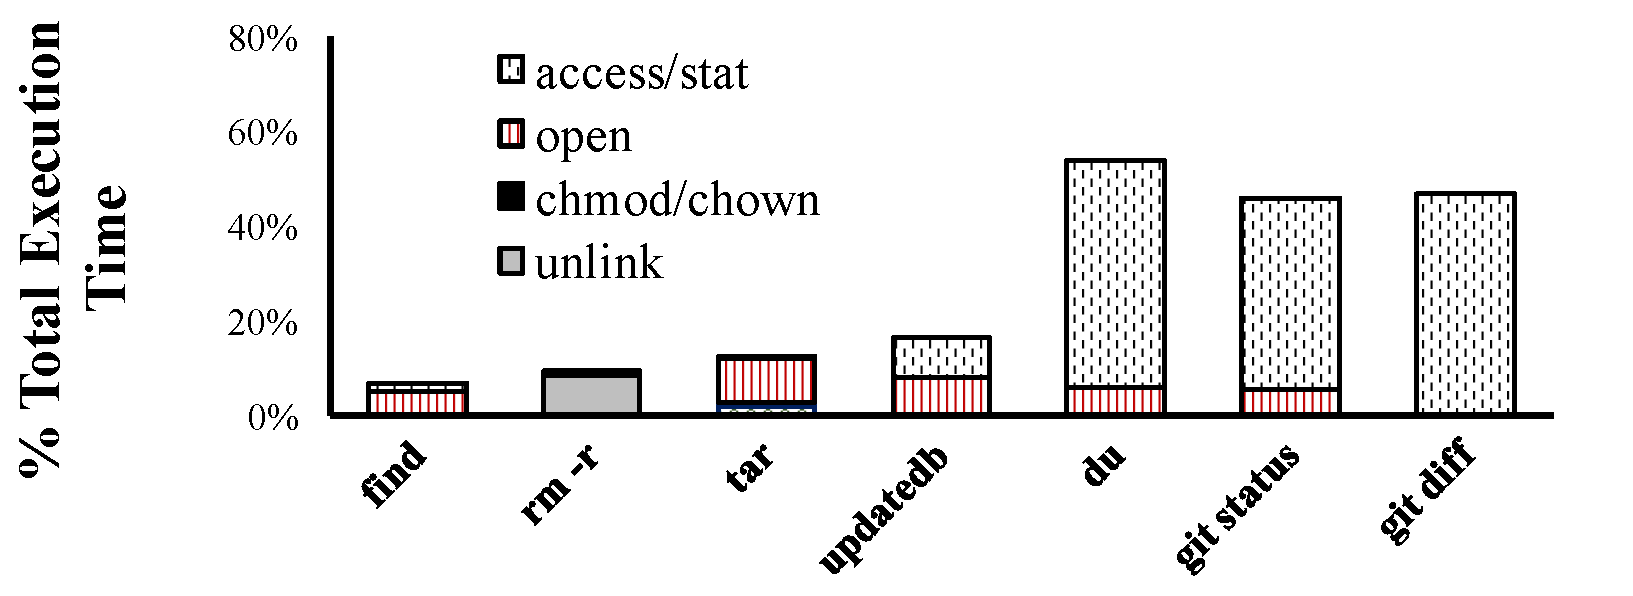
\includegraphics[width=5in]{dcache/plots/syscall-percentage.pdf} \\
\caption[Fraction of execution time on path-based system calls.]
{Fraction of execution time in several common utilities spent
executing path-based system calls with a warm cache, as measured with ftrace.}
\label{fig:dcache:lookup-frac}
%\vspace{-10pt}
\end{figure}

%\fixmedp{Please check these \% against time.  I think git diff is too high.  git status seems ok.}

Directory caches are essential for good application performance.
%Unix was designed such that ``(almost) everything is a file'',
%thus even accesses to in-memory file systems, device files, FIFOs and domain sockets
%first pass through the directory cache.
%In other words, 
Many common system calls must operate on file paths,
which require a directory cache lookup.
For instance, between 10--20\% of all system calls in the iBench system call traces do a path lookup~\citep{filenotafile}. 
Figure~\ref{fig:dcache:lookup-frac} lists the fraction of total execution time
%, as well as system time, 
several common command-line applications spend executing path-based system calls
(more details on these applications and the test machine in \S\ref{sec:dcache:eval}).
We note that these system calls include work other than path lookup,
and that these numbers include some instrumentation overhead;
% are coarse measurements that include  and work than path lookup;
%, and includes some time 
%for synchronous I/O (e.g., during {\tt rename}) as well as non-path tasks (e.g., creating 
%a file handle as part of {\tt open});
nonetheless, in all cases except {\tt rm},
the system call times and counts are dominated by
{\tt stat} and {\tt open}, for which 
%can be serviced from cache and for which 
path lookup is a significant component of execution time.
For these applications, path-based system calls account for 6--54\% of total execution time.
%and 25--77\% of system time.  
This implies that
lowering path lookup latency is
 one of the  biggest 
opportunities for a kernel to improve these applications' execution time.




\begin{figure}[t!]
\centering
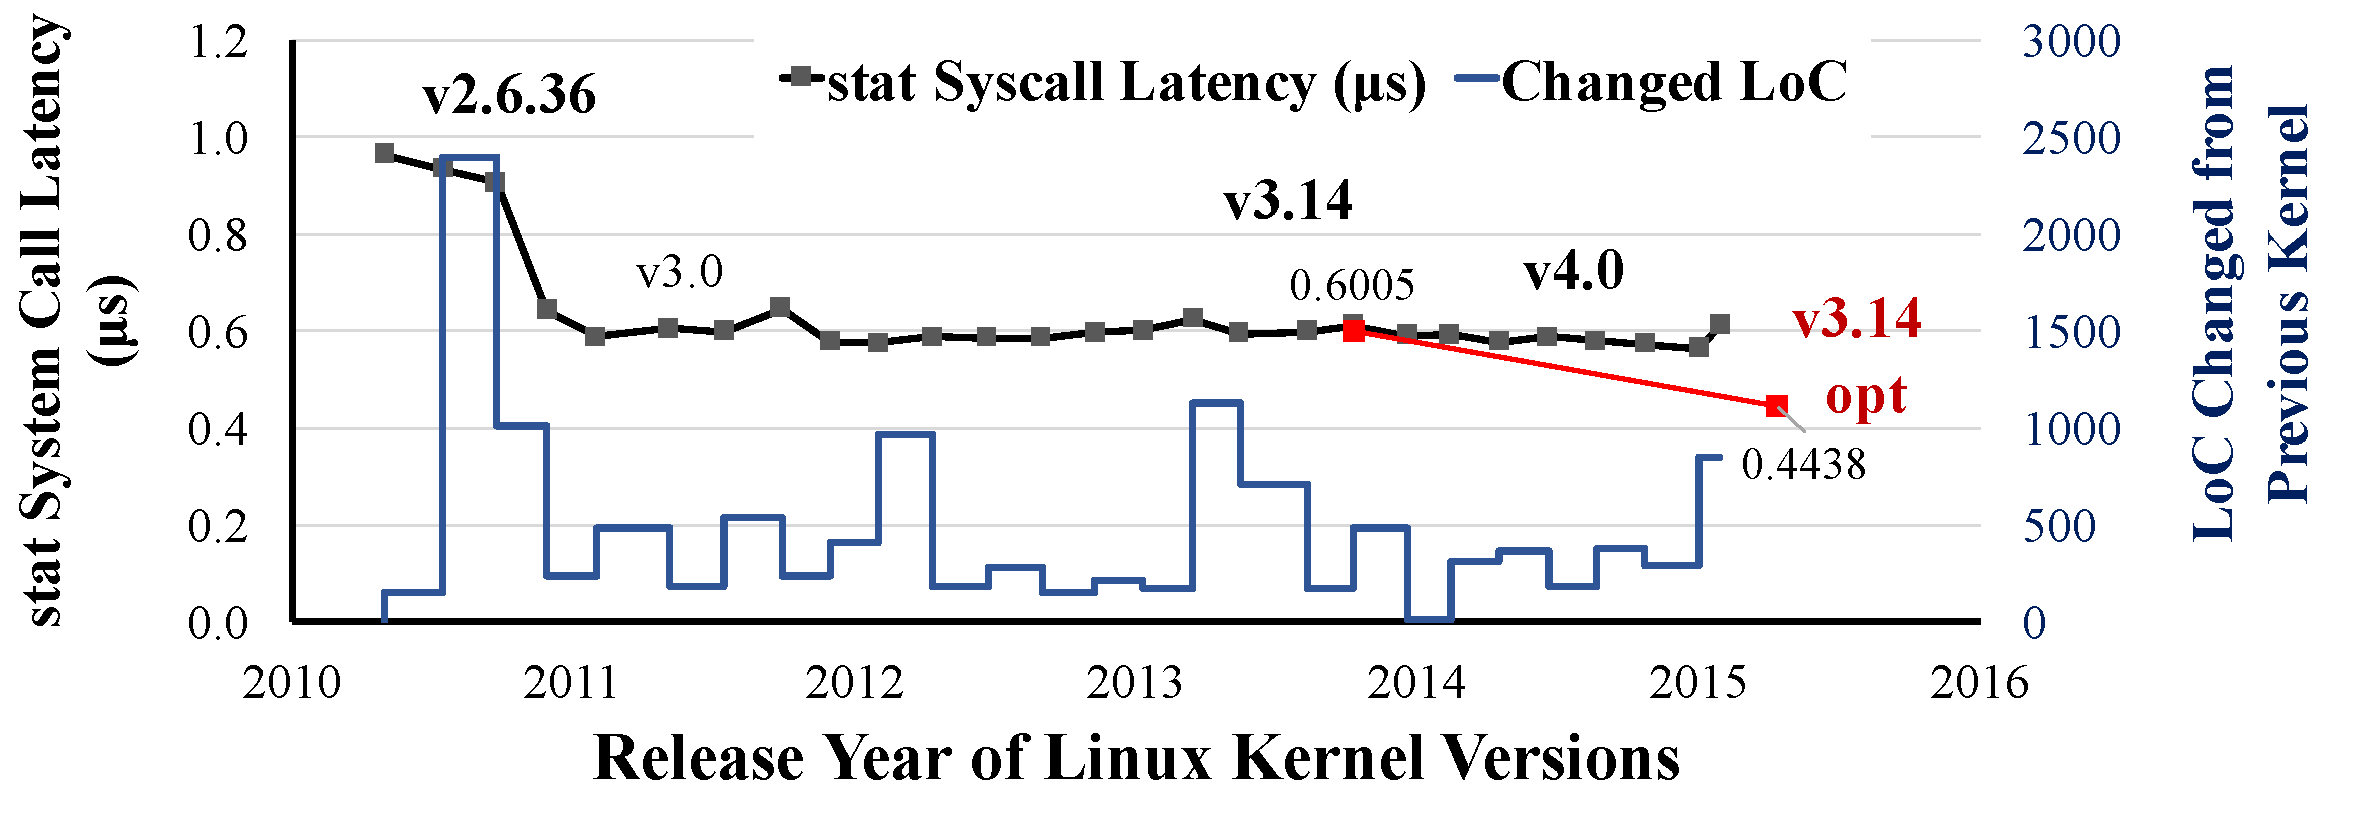
\includegraphics[width=6in]{dcache/plots/latency-by-version.pdf}
\footnotesize
\caption[Lantecy of {\tt stat} system call over years.]
{Latency of {\tt stat} system call with a long path {\tt XXX/YYY/ZZZ/AAA/BBB/CCC/DDD/FFF} on Linux over four years (lower is better), as well as the churn within the directory cache code (all insertions in {\tt dcache.c}, {\tt dcache.h}, {\tt namei.c}, {\tt namei.h} and {\tt namespace.c}). 
%Our optimizations significantly improve performance that has otherwise plateaued, despite significant ongoing developer effort.  
Our optimized \linuxver{} kernel 
further reduces {\tt stat} system call latency by \statspeedup{}\%.}
%\vspace{-15pt}
\label{fig:dcache:by-version}
\end{figure}


%\fixmedp{Add more evidence of lookup importance here: For instance, fraction of lookup time in file-related syscalls, or total lookup time in applications bound on file lookup latency.  }
Unfortunately, even directory cache hits are costly---0.3--1.1 \us{} for a {\tt stat} on our test Linux system, compared to only .04 $\mu$s for a {\tt getppid} and 0.3 \us{} for a 4 KB {\tt pread}. 
%\fixmetsai{Don, check this, I think read will be a better example, getppid is too trivial.}
This issue is taken particularly seriously in the Linux kernel community, which has 
made substantial revisions and increasingly elaborate optimizations to reduce the hit cost
of its directory cache, such as removing locks from the read path or replacing lock ordering with deadlock avoidance in a retry loop~\citep{corbet09jls,dcache-rcu}.
Figure~\ref{fig:dcache:by-version} plots directory cache hit latency against  lines of directory cache code changed 
over several versions of Linux, using a path-to-inode lookup \microbench{} on the test system described
in \S~\ref{sec:dcache:eval}.
These efforts have improved hit latency by 47\% from 2011 to 2013, but have plateaued
for the last three years.
%\fixmedp{if time, filter irrelevant changes from code deltas}
%at the cost of substantial developer effort.
%This latency appears to have plateaued 

The root of the problem is that the POSIX path permission semantics
seemingly require work that is linear in the number of path components,
and severely limit the kernel developer's implementation options.
%The root of this problem is that current directory cache
%designs reflect a straightforward implementation of the POSIX specification,
%which would seemingly require work that is linear in the number of path components.
For instance, in order to open file {\tt /\fnone{}/\fntwo{}/\fnthree{}} 
%for reading, 
one must have search permission
to parent directories {\tt /}, {\tt /\fnone{}}, and {\tt /\fnone{}/\fntwo{}},
as well as permission to access file {\tt \fnthree{}}.
The Linux implementation %of this specification is straightforward, 
simply walks the directory
tree top-down to check permissions.  
Unfortunately, when the critical path is dominated by 
walking a pointer-based data structure, 
including memory barriers on some architectures for multi-core consistency, 
modern CPUs end up stalling on hard-to-prefetch loads.
Moreover, because so many Linux features are built around this behavior, such as Linux Security Modules (LSMs)~\citep{wright+lsm},
namespaces, and mount aliases, it is not clear that any data-structural enhancements
are possible without breaking backward-compatibility with other Linux kernel features.
A priori, it is not obvious that a faster lookup algorithm, such as a single hash table lookup, 
can meet these API specifications and kernel-internal requirements; to our knowledge,
no one has tried previously.

%This paper proposes a decomposition of the directory cache, which allows
%most lookup operations to execute with a single hash table lookup (\S\ref{sec:dcache:dcache}),
%as well as optimizations to reduce the miss rate based on information that is {\em already in the cache}, but not used effectively (\S\ref{sec:dcache:readdir}).
%Our design maintains compatibility (\S\ref{sec:dcache:generalize}) through 
%several essential insights, including 
%how to separate the indexing of paths from checking parent permissions,
%and how to effectively and safely memoize the results of access control checks.


%% This paper proposes several new ways to organize a directory cache, which can yield 
%% substantial performance improvements over the current state of the art.
%% %This paper demonstrates that, despite this developer effort, there is still a substantial 
%% %missed opportunity hiding behind historical, intuitive, but not fundamental design choices.
%% Most of the Linux directory cache design reflects a straightforward implementation of the POSIX 
%% specification. %, with a division of labor that is suitable for mainstream file systems.

%This paper presents an alternative directory cache organization, which 
%improves performance by separating logical tasks, such as separating path indexing from permission checking; yet the design is sufficient to retain compatibility with POSIX.
%In the case of path lookup, 
%this paper demonstrates how 
%a per-component tree walk can be replaced with a single hash table lookup (\S\ref{sec:dcache:dcache}).
% without violating POSIX compliance.

%Our optimizations improve the performance of frequent lookup operations, but 
%introduce several costs, described in \S\ref{sec:dcache:dcache} and measured in \S\ref{sec:dcache:eval},
%which  we believe are acceptable and a net improvement for applications.
%First, these optimizations slow down infrequent modifications to the directory hierarchy, such as {\tt rename}, {\tt chmod},
% and {\tt chown} of a directory. 
%However, these slower operations
%account for less than .01\% of the system calls in the iBench traces~\citep{filenotafile}.
%Second,  the memory overheads of the dcache are increased.
%%(45\% per \dentry{}, as well as some  in our prototype).
%%(\fixmedp{XX MB} in our tests).  
%Third, lookup has a 
%probability of error from signature collisions that can be adjusted to be negligible
%%($2^{-141}$ in our configuration), 
%and within acceptable thresholds widely used by data deduplication systems~\citep{Debnath:2010:CSU:1855840.1855856, Srinivasan:2012:ILI:2208461.2208485, Quinlan:2002:VNA:645371.651321, Zhu:2008:ADB:1364813.1364831}.
%%, as well as how to remove
%%all memory barriers from the lookup path (\S\ref{sec:dcache:update}).
%In the micro-benchmark of Figure~\ref{fig:dcache:by-version}, our directory cache 
%optimizations improve lookup latency by 
%%revisions improve latency of accessing a long path
%%by 
%\statspeedup{}\% over unmodified Linux.
%%Our design addresses other missed
%%opportunities, such as identifying new opportunities to reduce the miss rate
%%through caching directory completeness.
%%\fixmedp{Do we want to highlight LoC?  3K is more than anything in the graph} \fixmetsai{Probably just mention in the evaluation. It's a metric that we should provide, but it's not awfully interesting.}
%%The total lines of code changed are fewer than 3,000 out of \fixmedp{XX}.
%%\fixmedp{Can we get 
%%, yet changes fewer than 3,000 lines of code.

%% SOSP cut - kind of long-winded
\begin{comment}
This paper rethinks current Linux directory cache design choices in light of the following goals:
\begin{compactitem}
\item {\bf Minimize the cost of a cache hit.} (\S\ref{sec:dcache:dcache}).
This means maximizing the benefit of temporal locality for frequent operations,
while pushing extra work of consistency maintenance onto less frequent, already-expensive operations.
%such as handling cache miss or updating massive metadata,
%in order to improve very frequent operations.
\item {\bf Maintain legacy compatibility.} (\S\ref{sec:dcache:generalize}).  Unix path semantics are complex, required by applications, file systems, and security modules, frustrating otherwise straightforward optimizations.  However tempting it may be to redesign path behavior to facilitate caching, path operations must exhibit the same behavior, with lower latency.
\item {\bf Never miss the same request twice in quick succession.} (\S\ref{sec:dcache:readdir}).  A number of less-frequent operations, such as reading a directory or secure temporary file creation, always miss in the cache {\em even if enough information is in cache to satisfy the operation.}  
%Of course, infrequent accesses should still be subject to a cache replacement policy, such as LRU.
\end{compactitem}
%Although directory caches must implement more complex semantics than a hardware memory cache,
%these principles should seem familiar to the reader with a basic architecture background.
%sadly, the Linux directory cache design violates all three.
\end{comment}

%This paper introduces several techniques to improve the performance of a directory cache,
%This paper explains several practical directory cache optimizations,
This paper demonstrates that these techniques improve performance for applications that use the directory cache heavily,
and the harm is minimal to applications that do not benefit.
%and that the worst case \microbench{} is only 12\% slower within \fixmedp{XX}\% of unmodified Linux.
%Each optimization we describe improves performance in isolation, and all can be combined.
%These optimizations change very few lines of code, and are backward-compatible with 
%legacy applications.  
%These changes are encapsulated in the VFS---individual file systems do not have to change their code.
%This paper describes a  prototype of these improvements implemented in Linux \linuxver{}.
%\S~\ref{sec:dcache:background} explains that the directory cache structure of Mac OS X, FreeBSD, and Solaris 
%are sufficiently similar that these principles should generalize.
%we compare and contrast Linux's directory cache
%with Mac OS X, FreeBSD, and Solaris in \S\ref{sec:dcache:background}, and explain inline how each
%optimization could be generalized to these other OS kernels.





%% \item {\bf Modularization and stackability}:
%% Any changes or optimizations must be implemented as modules inside Linux's VFS,
%% and can be stacked on top of the original design or any future optimizations. 
%% \item {\bf Backward compatibility}:
%% Any changes or optimizations must maintain least requirement of modifying any
%% file systems.
%% \item {\bf Generalization to other OSes}: Any changes or optimizations must be portable to other OSes with reasonable effort and change of design.




%% \dcache{} is proven to be effective on improving storage performance.
%% Experiments shows that,
%% in a Linux 3.x kernel, a \dcache{} with a xxx\% hit rate can speed up
%% metadata lookup and fetching time by xxx times.
%% \fixmetsai{experiment result, Linux version, and fs specs here}
%% However, we observed that Linux maintainers have made
%% constant and non-trivial efforts to improve \dcache{} in the Linux kernel.
%% We studied all \dcache{}-related source files in the Linux kernel Git repository,
%% and discovered that maintainers have committed
%% on average xxx revisions per source files.

%% We tested metadata lookup time on primary \dcache{}-related revisions.
%% Most changes on \dcache{} system only create xxx\%-xxx\% speed-up
%% than their predecessor.
%% \fixmetsai{result and graph here}.
%% Moreover, improvement to \dcache{} is still work-in-progress
%% for Linux maintainers.
%% \fixmetsai{reference to threads for latest dcache discussions}. 
%% All the evidences show that,
%% despite of significant reduction of storage operations,
%% efficiency of \dcache{} system internally still remains as a concern.

%% We argue that the design of \dcache{} needs to be carefully re-examined,
%% to fundamentally identify any missed opportunities that
%% improve value of \dcache{}.
%% At a high level, most optimization works for \dcache{} are focused on
%% improving ``how to cache'',
%% but we want to also lay eyes on ``what to cache'',
%% to ensure any valuable information returned from file systems
%% be captured by \dcache{} system.

%The contributions of this paper are as follows:
%\begin{compactitem}
%\item A performance analysis of the costs of path lookup and the opportunities
%to improve cache hit latency.
%\item A directory cache design that improves path lookup latency with a combination of techniques, including:
%  \begin{compactitem}
%  \item Indexing the directory cache by full path, reducing average-case lookup from linear to constant in the number of path components.
%  \item A Prefix Check Cache (PCC) that separates permission checking from path caching.  The PCC memoizes permission checks, and is compatible with LSMs~\citep{wright+lsm}.
%  \item Reducing the cost of checking for hash bucket collisions with path signatures.
%  \end{compactitem}
%\item Identifying opportunities to leverage metadata the kernel already has to reduce miss rates, such as tracking whether a directory is completely in cache.
%\item Carefully addressing numerous, subtle edge cases that would frustrate rote application of these techniques, such as integration with symbolic links and Linux namespaces.
%\item A thorough evaluation of these optimizations.  For instance, our optimizations improve throughput
%of the Dovecot IMAP server by up to \dovecotspeedup\% and latency of 
%updatedb by up to \updatedbspeedup{}\%.
%%git version control system by up to 25\%.
%
%\end{compactitem}

\section{API compatibility metrics}
\label{sec:metric:definitions}

We started this study from a research perspective, in search of a better way to evaluate
the completeness of system prototypes with a Unix compatibility layer.
In general, compatibility is treated as a binary property
(e.g., bug-for-bug compatibility), which loses 
important information when evaluating a prototype that is almost certainly incomplete.
Papers often appeal to noisy indicators that the prototype probably covers all important use cases,
such as the number of total supported system or library calls, as well as the variety
of supported applications.


These metrics are easy to quantify, but problematic.
Simply put, not all APIs are equally important: some are indispensable (e.g., \syscall{read} and \syscall{write}),
whereas others are very rarely used (e.g., \syscall{preadv} and \syscall{delete\_module}).
A simple count of system calls is easily skewed by 
system calls that are variations on a theme (e.g., \syscall{setuid}, \syscall{seteuid}, and \syscall{setresuid}).
Moreover, some system calls, such as \syscall{ioctl},
export widely varying operations---some used by 
by {\em all} applications and many that are essentially never used (\S\ref{sec:study:opcodes}).
%We use the term {\em vectored system call} for calls, such as {\tt ioctl},
%which essentially export a nested system call table, selected by an opcode argument.
%by {\em any} applications in Ubuntu 
Thus, a system with ``partial support'' for \syscall{ioctl}
is just as likely to support all or none of the Linux applications distributed with Ubuntu.



%This paper considers system APIs (``APIs'') broadly:
%this includes system calls, as well as any other means by which OS kernel functionality is
%requested, such as a pseudo-file system ({\tt /proc}).
%This paper also considers
%libraries like libc, which are typically responsible for exporting an API, like POSIX,
%as well as the primary way application developers interact with the OS kernel.
%For applications, system libraries are also system APIs. Modern applications rarely use the kernel interfaces like system calls directly, but instead call library APIs as wrapper or translation layer of kernel interfaces. 
%For Linux platforms, \libc{}, or {\em Standard Library C}, is the most ubiquitously used system libraries, providing a large fraction of
%general-purpose APIs commonly used by every application.


%%%  for the rest of the paper) as channels upon which
%%% applications request system functionalities,
%%% based on the contract between users and OS developers.
%%% The basic form of APIs on UNIX platforms is the system call,
%%% but others exist.
%%% For example, other APIs can be used through accessing system pseudo files or devices,
%%% such as {\tt /proc} files,
%%% or even communicating with administrative services using specific protocols (not covered in this paper).
%%% Although a API can contain multiple channels ---
%%% for instance, {\tt stat} system call provides several file attributes, or a pseudo file can be either read or written ---
%%% we group the usage data by system call numbers, vectored system call operation codes, and file paths,
%%% as the basic granularities of our analysis.  



%and easy to miss important cases in single system calls with a wide variety of options, such as {\tt ioctl}.

One of the ways to understand the importance of a given interface
is to measure its impact on end-users.  
In other words, if a given interface were not supported, how many users would notice its absence?
Or, if a prototype added a given interface, how many more users would be able to use the system?
%% probably don't need this note to Bianca
%\note{Drop footnote here.}
%\footnote{This assumes that the prototype is well-supported by the developers, and the maintainers have reasonable
%  installation instructions, are responsive to bug reports, etc.  The issues around maturity and support
%  of research prototypes are orthogonal to the question of which APIs need to be present
%  in a proof-of-concept system.}
To answer these questions, we must consider both the 
difference in API usage
among applications,
and the popularity of applications among end-users.
We measure the former by analyzing application binaries,
and determine the latter from installation statistics collected
by Debian and Ubuntu~\citep{ubuntu-popularity,debian-popularity}.
An {\bf installation} is a single system installation, and can 
be a physical machine, a virtual machine, a partition in a multi-boot system,
or a chroot environment created by {\tt debootstrap}.
Our data is drawn from over 2.9 million installations
(2,745,304 Ubuntu and 187,795 Debian).
%\fixmedp{Add a summary about how big this data set is (i.e., millions of systems)}
%Although difficult to measure directly, we approximate this based on package installation statistics~\citep{ubuntu-popularity}.


%%% This paper borrows the notion of installations from the package installation statistics.
%%% An {\em installation} represents a set of software installed in a standalone environment
%%% using the provided Ubuntu or Debian package installer.
%%% An installation does not necessarily represent a physical machine;
%%% it can be a partition in a multi-boot system,
%%% a virtual machine,
%%% or even a subsystem installed by 

We introduce two new metrics: one for each API, and one for a whole system.
For each API, we measure how disruptive its absence
would be to applications and end users---a metric we call {\bf  \usagemetric{}}.
For a system, we compute a weighted percentage we call {\bf \compatmetric{}}. 
For simplicity, we define a {\bf system} as a set of implemented or translated APIs,
and assume an 
application will work on a target system if the application's API footprint is implemented on the system.
These metrics can be applied to all system APIs,
or a subset of APIs,
such as system calls 
or standard library functions.
%pseudo-file system interfaces ({\tt /proc}),
%device interfaces ({\tt /dev}), or standard library functions.
%These metrics , and is fully generalizable to other families of OS distributions.



This paper focuses on \osdist{}, as it is a well-managed Linux distribution with a wide array of 
supported software, which also collects
package installation statistics.
The default package installer on \osdist{} is \osinstaller{}.
A {\bf package} is the smallest granularity of installation, typically
matching a common library or application.
A package may include
multiple executables, libraries, and configuration files.
Packages also track dependencies, such as a package containing 
Python scripts depending on the Python interpreter.
%Note that a package may install multiple executables,
%but the granularity of a package
%typically matches a single application or a set of 
%common, supporting libraries.
%one or more application binaries, but installation statistics are only collected
%at package granularity.
\osdist{} installation statistics are collected at package granularity
and collect several types of statistics.
This study is based on
data of how many
Ubuntu or Debian installations
installed a given target package.
%Other installation statistics are ignored,
%because they do not provide complete information about users' actual choices of packages.}
%\byinst{} shows how many systems installed the package,
%and \byvote{} shows how many systems regularly use the package.
%We calculate our measurements based on both data, depending on
%whether one is interested in supporting
%{\it all} packages installed on a system, or prioritizing {\it important} packages.

%%% For a system, a package is the smallest unit of installation.
%%% %by the package installer.
%%% Each package is a set of files that will be placed into the
%%% file systems. %when the package is installed.
%%% Note that a package does not always include standalone executables.
%%% Other files that can be found in a package
%%% includes scripts, shared libraries, configuration files,
%%% or even kernel extensions (modules).
%%% For those packages that do not include executables,
%%% our study tracks their dependencies. %of those packages.
%%% For example, a package containing Python scripts will depend on
%%% the Python package.
%%% We mark both packages as compatible if Python itself is supported.



For each binary in a package---either as a standalone executable or shared 
library---we use static analysis to identify all possible APIs the binary could call,
or the {\bf API footprint}.
The APIs can be called from the binaries directly,
or indirectly through calling functions exported by other shared libraries.
A package's API footprint is the union of the API 
footprints of each of its standalone executables.
We weight the API footprint of each package by its installation frequency
to approximate the overall importance of each API.
%Based on installation statistics of the package, we approximate the transitive importance of the system calls in each binary's footprint.
Although our initial focus was on evaluating research,
our resulting metric and data analysis provide insights for
the larger community, such as trends in API usage.



% Bug-for-bug compatibility beyond our scope; techniques largely orthogonal to this study; we assume that, once a given system call (say write) is supported and works for a reasonable sample of applications, handling edge cases should be straightforward engineering.  That said, for system calls 

%%% Put current metric discussion here

%% Then a subsection on approach and assumptions



\begin{comment}
API compatibility is one of most important system properties, for maintaining the availability of the whole system and decoupling the development of the OS and every applications.
For an OS of the size of Linux or Microsoft Windows, millions of softwares and subsystems are implemented on top of the platform,
counting on the API contracted to provide its services.
If a system engineer decides to change the API,
an inevitable risk is to sweep and update every existing applications accordingly, which are designed and maintained by countless third parties in the world.

Then, why would a system engineer try to change the API of an OS?
The answer is related with the procedure of developing an OS.
When an OS prototype is built, developers have to rely on experiences and instincts to make educated guess about what to be the ideal API of the system.
As time goes by, the OS gains a larger user base, and receives feedbacks about how the API should really be designed.
As soon as a developer realizes that refining the API can effectively improve either efficiency, robustness, security or user-friendliness of the system,
the risk of losing compatibility {\em slightly} can be totally worthy.

Unfortunately, the reality is that system engineers are frighten by the cost of refining the API for being unable to know how compatibility can be effected.
Since there is no data set about the actual usage of the API among applications, they must assume any application developers can potentially depend on the API.
It often takes a very long time, says 6 years \fixmetsai{LSB took 6 years, reference?}, to confirm, announce, communicate or simply wait until the API is officially deprecated.

We argue that knowing the API usage is the first step of understanding and evaluating compatibility.
Instead of using a realistic metric, system engineers often express the affects on API compatibility by numbers of interfaces that are implemented or modified.
Evaluation by counting the interfaces is extremely inaccurate, because every part of the API have different importance among applications.
Some interfaces are simply more frequently used and thus more important than others; for example, the consequence of changing system call {\tt open}, which is used ubiquitously,  is not the same as changing others like {\tt msgget}.
\end{comment}


\begin{comment}
%Bhushan: - Begin here -
Knowing the values of system interfaces among users is the prerequisite of evaluating platform compatibility.
When OS developers test their systems, a common approach is to prepare numerous test cases that exercise individual system interfaces.
It is often a natural thing to do for OS developers to maintain a list of supported system interfaces,
for either development purpose or advertisement.
However, because system interfaces have different values for users, they cannot be equal while evaluating platform compatibility of the OS.
A frequently used system interface should be considered more important for compatibility than a rarely used one.
\end{comment}

\subsection{\Usagemetric{}}

System developers can benefit from an importance metric for APIs,
which can in turn guide optimization efforts, deprecation decisions,
and porting efforts.  
Reflecting the fact that users install and use different software packages,
%Because users install different software on different systems, 
we define
\usagemetric{} as the probability that
an API will be indispensable to 
 at least one application on a randomly selected 
installation.
We want a metric that decreases
as one identifies and removes instances
of a deprecated API,
and a metric that will remain high for an indispensable API, 
even if only one ubiquitous application uses the API.



%, the  of that API will decrease.
%Similarly, an \usagemetric{} near 100 percent indicates an API is indispensable,
%at least for one ubiquitous application.
%The unsupported API with the highest \usagemetric{} creates an upper bound on 
%the system's overall  \compatmetric{}.
%For instance, if a system is missing an API with an \usagemetric{} of 20\%,
%the \compatmetric{} will never be higher than 80\% (but could be significantly lower).


%%% Given a complete list of installed applications in an OS installation,
%%% by examining the API footprint of every application,
%%% we can easily determine whether removing an API is disruptive for such an installation.
%%% %The result is a binary property: whether the API is important to
%%% %the installation or not.
%%% However, it is hard to predict what applications an installation will include.
%%% Thus, we define the metric for API usage as the probability
%%% that that target API
%%% is indispensable for an random installation.

%\vspace{0.1in}
%{\noindent
%\fbox{\begin{minipage}{\linewidth}
%\setlength{\parindent}{-0.1in}
%\setlength{\leftskip}{0.1in}
%\setlength{\rightskip}{0.1in}
% Definition: {\bf \UsageMetric{}.} \\
%For a given API, the probability that an installation includes
%at least one application requiring the given API.
%at least one broken application
%(whose API footprint covers the target API),
%if the target API was removed.
%\end{minipage}}}
%\vspace{0.1in}

\noindent Intuitively, if an API is used by no packages or installations,
the \usagemetric{} will be {\em zero}, causing no negative effects if removed.
We assume all packages installed in an OS installation are indispensable.
As long as an API is used by at least one package,
the API is considered {\it important} for the installation.
Appendix \ref{sec:defs:usagemetric} includes a formal definition of \usagemetric{}.
 
%% Besides the metric, the popularity of system interfaces can be important development hints as well.
%% Knowing the most and least valuable system interfaces of an OS,
%% the developers can make better decision on prioritizing the maintenance or retirement of the interfaces.
%% More influences of system interface popularity are discussed in \fixmetsai{later section?}.

%We define the popularity of a system interface by the probability that an installation become unsupported if the interface is removed.
%In other word, the popularity indicates the {\em cost} or {\em penalty} of deprecating an interface.

\begin{comment}
\paragraph{Formal Definition.}
A given system installation ($\mathtt{Inst}$)
is a set of packages installed ($\{\mathtt{pkg}_1, \mathtt{pkg}_2, ..., \mathtt{pkg}_k \in \mathtt{Pkg}_\mathtt{all}\}$).
For each package $\mathtt{pkg}$ in the \osdist{} repository,
our framework generates the API footprint as 
${\mathtt{Footprint}}_\mathtt{pkg} = \{\mathtt{api}_1, \mathtt{api}_2, ..., \mathtt{api}_k \in \mathtt{API}_\mathtt{all}\}$.  
For an API supported by the OS, we calculate the \usagemetric{} as the product 
of probabilities that an installed package will require this API.
This is calculated as follows:
\begin{align*}
&\mathtt{Dependent}_\mathtt{api} = \{\mathtt{pkg}|\mathtt{api} \in \mathtt{Footprint}_\mathtt{pkg}\} \\
&\mathtt{Importance}(\mathtt{api}) = Pr\{\mathtt{Dependent}_\mathtt{api} \bigcap \mathtt{Inst} \neq \emptyset\} \\
&= 1 - Pr\{\forall \mathtt{pkg} \in \mathtt{Dependent}_\mathtt{api}, \mathtt{pkg} \notin \mathtt{Inst}\} \\
&= 1 - \prod_{\mathtt{pkg} \in \mathtt{Dependent}_\mathtt{api}} Pr\{\mathtt{pkg} \notin \mathtt{Inst}\} \\
&= 1 - \prod_{\mathtt{pkg} \in \mathtt{Dependent}_\mathtt{api}} (1 - \frac{\text{installation of $\mathtt{pkg}$}}{\text{total installation}})
\end{align*}
\end{comment}


\subsection{\Compatmetric{}}

We also measure compatibility at the granularity of an OS,
which we call \compatmetric{}.
\Compatmetric{} is the fraction of applications that are likely to work,
weighted by the likelihood that these applications will be installed on a system.
%\fixmedp{check this synopsis}
% function of the APIs supported, weighted by the popularity 
%of the applications that require these APIs.

The goal of \compatmetric{} is to measure the degree to which a
new OS prototype or translation layer is compatible with a baseline OS.
In this study, the baseline OS is \osdist{}.



%%  as a function of the API footprint of each potentially-installed
%% application, weighted by the popularity of each application.
%% We introduce the metric , which we define in terms of an OS installation (i.e.,
%% the libraries and applications) and a target API implementation, which may provide a subset
%% of the original system's APIs.


%% An accurate metric for API compatibility must take into account at least two factors:
%% \begin{compactenum}
%% \item For each interface in the API, what are the applications that rely on it and could be affected if the interface is removed? ({\em application footprint})
%% \item For each application, how many installations of the system in the world has included it? ({\em application popularity})
%% \end{compactenum}


%% \fixmedp{Term for each call, vs system overall: API Importance and Effective Coverage?}

%% To accurately evaluate compatibility, we design a metric that is quantifiable, \fixmetsai{one more word here}, and easy to interpret.

\begin{comment}
We defined {\bf platform compatibility} as "{\em the probability of porting any installation of an OS distribution onto the target OS without any effort}".
The definition of an {\em installation} is a combination of application setup on a standalone OS instance.
An Installation can exist on physical machines,
or any machines of generalized sense such as a virtual machines, containers or subsystems.
In our model, installations represent customers of the OS, who are considered equal when providing any services.
\end{comment}

%\vspace{0.1in}
%\fixmetsai{Find a good name for our metric} 
%{\noindent
%\fbox{\begin{minipage}{\linewidth}
%\setlength{\parindent}{-0.1in}
%\setlength{\leftskip}{0.1in}
%\setlength{\rightskip}{0.1in}
%Definition: {\bf \CompatMetric{}.} \\
%For a target system, the fraction of applications supported,
%weighted by the popularity of these applications.
%For any installation, the expected fraction of installed applications that can work on the target OS.
%\fixmedp{shouldn't the weight go in the definition?}
%\Compatmetric{} is the total size of all supported applications,
%weighted by the popularity of each application.
%\end{minipage}}}
%\vspace{0.1in}

%\noindent In terms of porting effort, we are primarily interested in avoiding code changes, 
%such as {\tt \#ifdef LINUX}; although we leave this notion somewhat vague.
%We consider recompilation, relinking, or other mechanical processes acceptable.

%% Our analysis framework scans through all available packages in the \osdist{} repository and generates system interface footprint data for individual package.
%% The footprint data is based on static analysis,
%% and it lists all potentially used system interfaces regardless of the applications' runtime coverage. 
%% To build the metric, we also import the package popularity statistics from the official \osdist{} reports~\citep{ubuntu-popularity, debian-popularity}.

The methodology for measuring the \compatmetric{} of a target system's API subset is summarized as follows:
\begin{compactenum}
\item Start with a list of supported APIs of the target system, either identified from the system's source, or as provided by the developers of the system.
\item Based on the API footprints of packages, the framework generates a list of supported and unsupported packages.
\item The framework then considers the dependencies of packages. If a supported package depends on an unsupported package, both packages are marked as unsupported.
\item Finally, the framework weighs the list of supported packages based on package installation statistics.
As with \usagemetric{}, we measure the effected package that is most installed;
\compatmetric{} instead calculates the expected fraction of packages in a typical installation that will work on the target system.
%Specifically, each package's weight is based on 
%and the framework calculates the expected fraction of packages from a typical installation that will work on the target system.
\end{compactenum}
%\fixmedp{``typical installation'' raised some hackles.  Can we either use a different term, or talk more about this concept?}

\begin{comment}
\paragraph{Formal Definition.}
Suppose an OS supports a set of APIs ($\mathtt{API}_\mathtt{Supported}$),
% = \{i_1, i_2, ..., i_n\}$
which is a subset of the APIs of the original system ($\mathtt{API}_\mathtt{all}$).
In this study, $\mathtt{API}_\mathtt{all}$ is the sum of Linux APIs, including
the system call table, sysctl, proc, and so forth.
%(total APIs are $\Sigma = \{i_1, i_2, ..., i_m\}, m \geq n$).
A list of supported packages ($\mathtt{Pkg}_\mathtt{Supported}$) can be generated by checking whether the API footprint is
a subset of the target system's supported APIs ($\mathtt{API}_\mathtt{Supported}$):
\begin{align*}
\mathtt{Pkg}_\mathtt{Supported} = \{\mathtt{pkg} | \mathtt{Footprint}_\mathtt{pkg} \subseteq \mathtt{API}_\mathtt{Supported}\}
\end{align*}
\end{comment}


\vspace{10pt}
We note that this model of a typical installation is useful in reducing the metric to a single number,
but also does not capture the distribution of installations.
This limitation is the result of the available package installation statistics,
which do not include correlations among installed packages.
%Using package installation statistics has the important limitation that 
%which package installations are correlated.
This limitation requires us to 
assume that package installations are independent,
except when \osinstaller{} identifies a dependency.
For example, if packages {\em foo} and {\em bar} are both reported as being installed once,
we cannot tell if they were on the same installation, or if two different installations.
If foo and bar both use an obscure system API, we assume that two installations would be affected if the obscure API were removed.
If foo depends on bar, we assume the installations overlap. % overlapping installations are on the same system.
%We note that packages do include installation dependences, which could be used in future work to reduce this over-approximation.
%\fixmedp{Check my edit: I was confused by the old wording}
Appendix \ref{sec:defs:compatmetric} formally defines \compatmetric{}.



%% In our experiment, we assume installation of any packages to be {\em independent events}.
%% This is a strong assumption that can affect the precision of the metric.
%%  We introduce the assumption for the following reasons:
 
%%  \begin{compactenum}
%%  \item The official \osdist{} package popularity reports contain no relative popularity between packages. Neither is the raw data of individual installation published. 
%%  \item Most of the packages depend on others due to library dependency. Our analysis combines the popularity among libraries into the statistics of executables, and only counts executables for evaluation. 
%%  \end{compactenum}
 
%% As a limitation, we do not consider the case where executables may have relative popularity due to users' preference. For example, Apache-PHP-Mysql is a combination installed on many machines that provide web services.
%% In our experiment, we assume installation of each package is irrelevant with others.

\begin{comment}
Formally, \compatmetric{} is the expected fraction of packages on a given system($\mathtt{Inst}$)
having an API footprint within the target 
system's supported APIs.
%We approximate the expected value as follows:
%Based on the list of supported packages, we can calculate the probability of an installation $\zeta = \{p^{\zeta}_1, p^{\zeta}_1, ..., p^{\zeta}_q\}$ to be fully compatible as follows:
By assuming independence of package installation, we can calculate the probability of supporting an installation as follows:
\begin{align*}
&\mathtt{Weighted Compliance}(\mathtt{API}_\mathtt{Supported}) =\\
&E(\frac{|\mathtt{Pkg}_\mathtt{Supported} \bigcap \mathtt{Inst}|}{|\mathtt{Inst}|}) \sim \frac{E(|\mathtt{Pkg}_\mathtt{Supported} \bigcap \mathtt{Inst}|)}{E(|\mathtt{Inst}|)} \\
&\sim \frac{\sum_{\mathtt{pkg} \in \mathtt{Pkg}_\mathtt{Supported}} (\frac{\text{installation of $\mathtt{pkg}$}}{\text{total installation}})}{\sum_{\mathtt{pkg} \in \mathtt{Pkg}_\mathtt{all\hspace{0.21in}}} (\frac{\text{installation of $\mathtt{pkg}$}}{\text{total installation}})} \\
&\text{where E}(\mathtt{x})\text{ is the Expectation of }\mathtt{x}\text{ occurring.}
\end{align*}
\end{comment}

%% dp:Meh
%\subsection{Justifying the Practicability of the Metric}

\section{Data collection}
\label{sec:metric:collection}

We use static binary analysis to identify the system call footprint of a binary.  This approach has the advantages
of not requiring source code or test cases.  Dynamic system call logging using a tool like {\tt strace} is simpler,
but can miss input-dependent behavior.  A limitation of our static analysis is that we must assume the disassembled binary
matches the expected instruction stream at runtime.  In other words, we assume that the binary isn't deliberately obfuscating
itself, such as by jumping into the middle of an instruction (from the perspective of the disassembler).
%In practice, such obfuscation is generally done only by malware, and our results are not concerned with system security.
To mitigate this, we spot check that static analysis returns as superset of {\tt strace} results.

We note that, in our experience, things like the system call number or even operation codes are fairly straightforward
to identify from a binary.  These tend to be fixed scalars in the binary, whereas other arguments, such as the contents of a write buffer,
are input at runtime.
We assume that binaries can issue system calls directly with inline system call instructions, or can call system calls through a library, such as \libc{}.
Our static analysis identifies system call instructions and constructs a whole-program call graph.

\begin{figure}[t!]
\centering
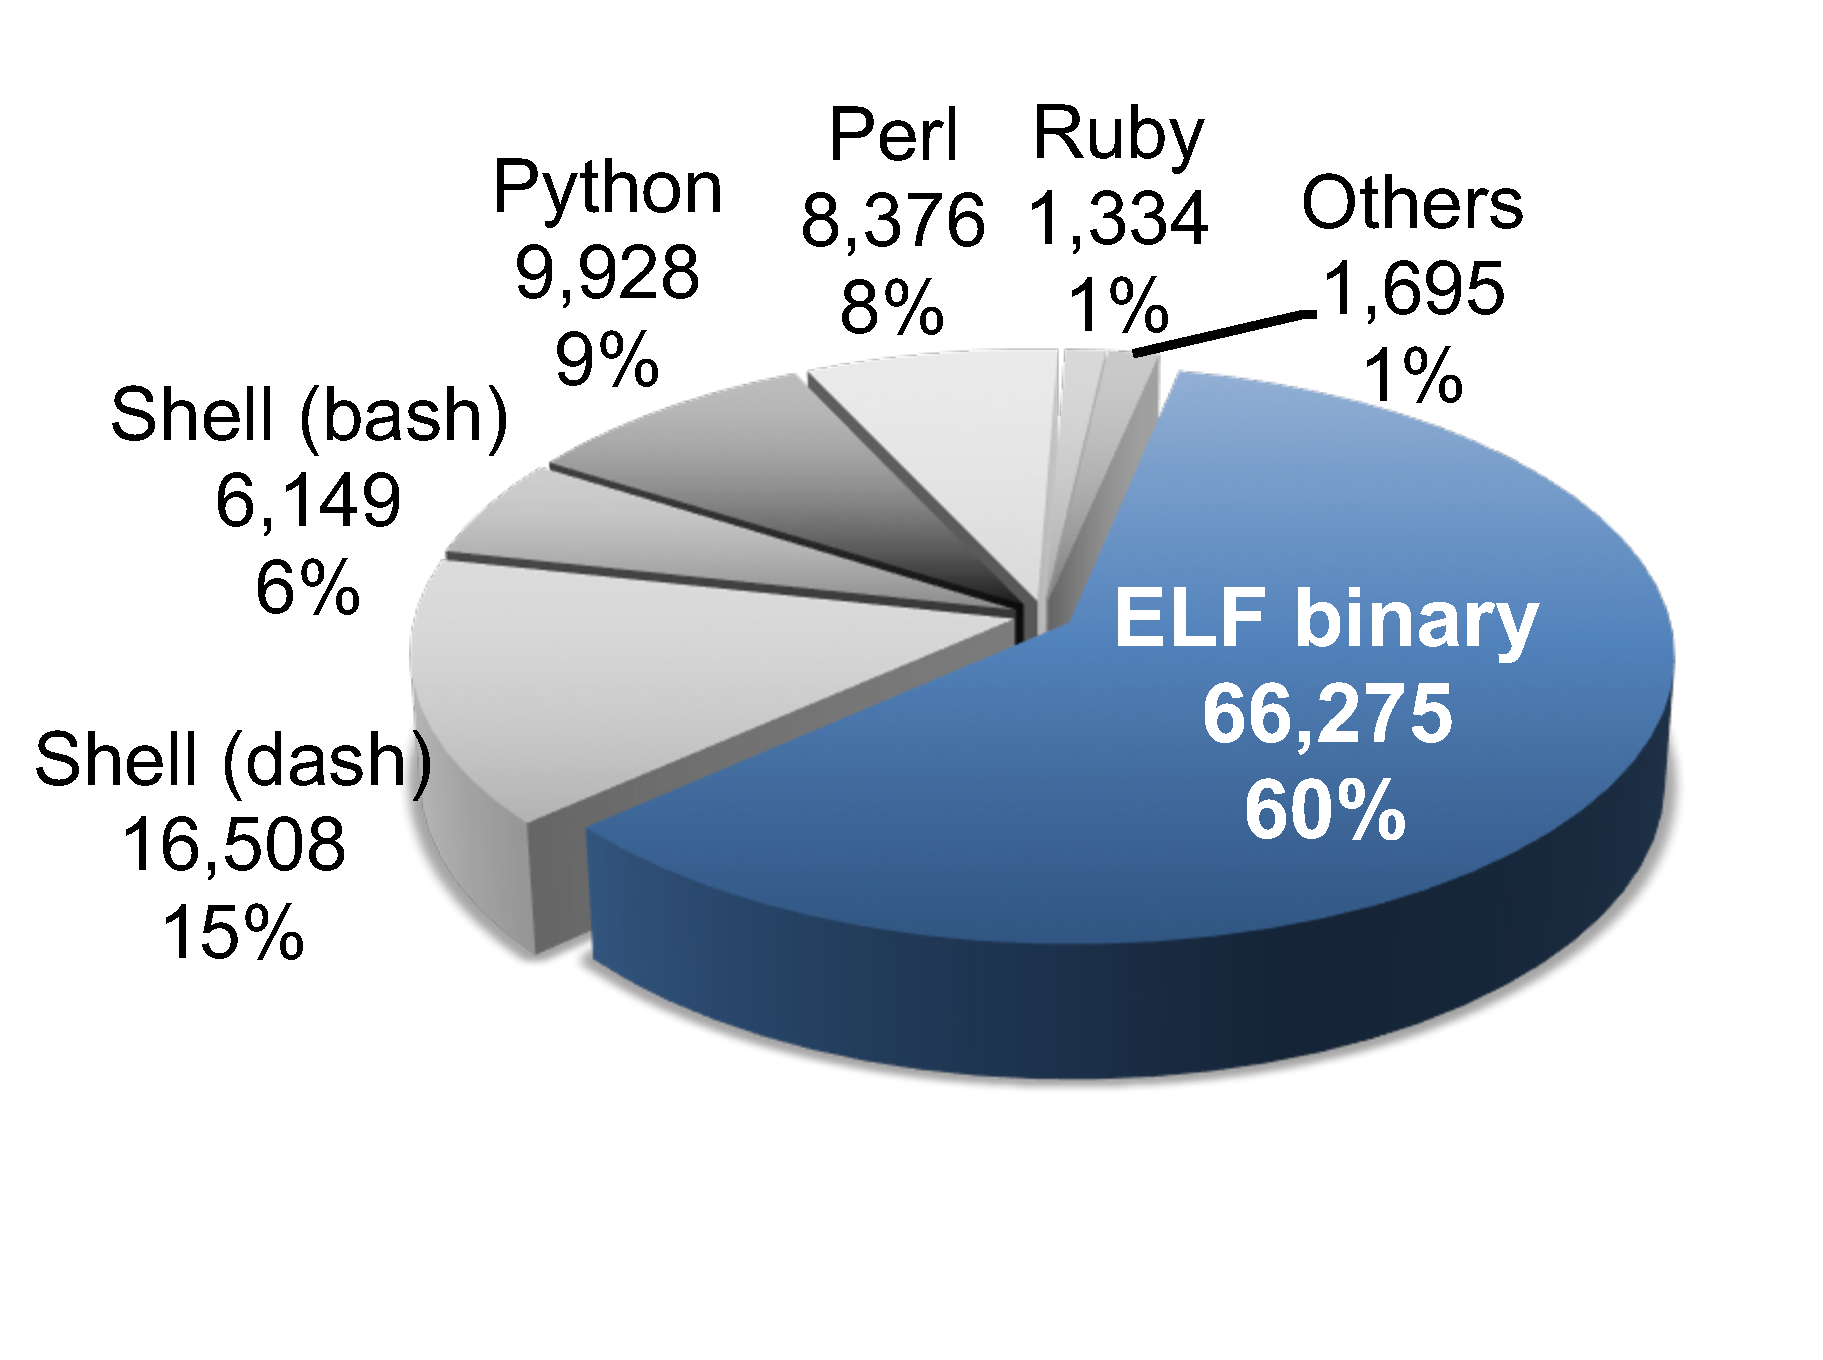
\includegraphics[width=3.2in]{executable-type.pdf}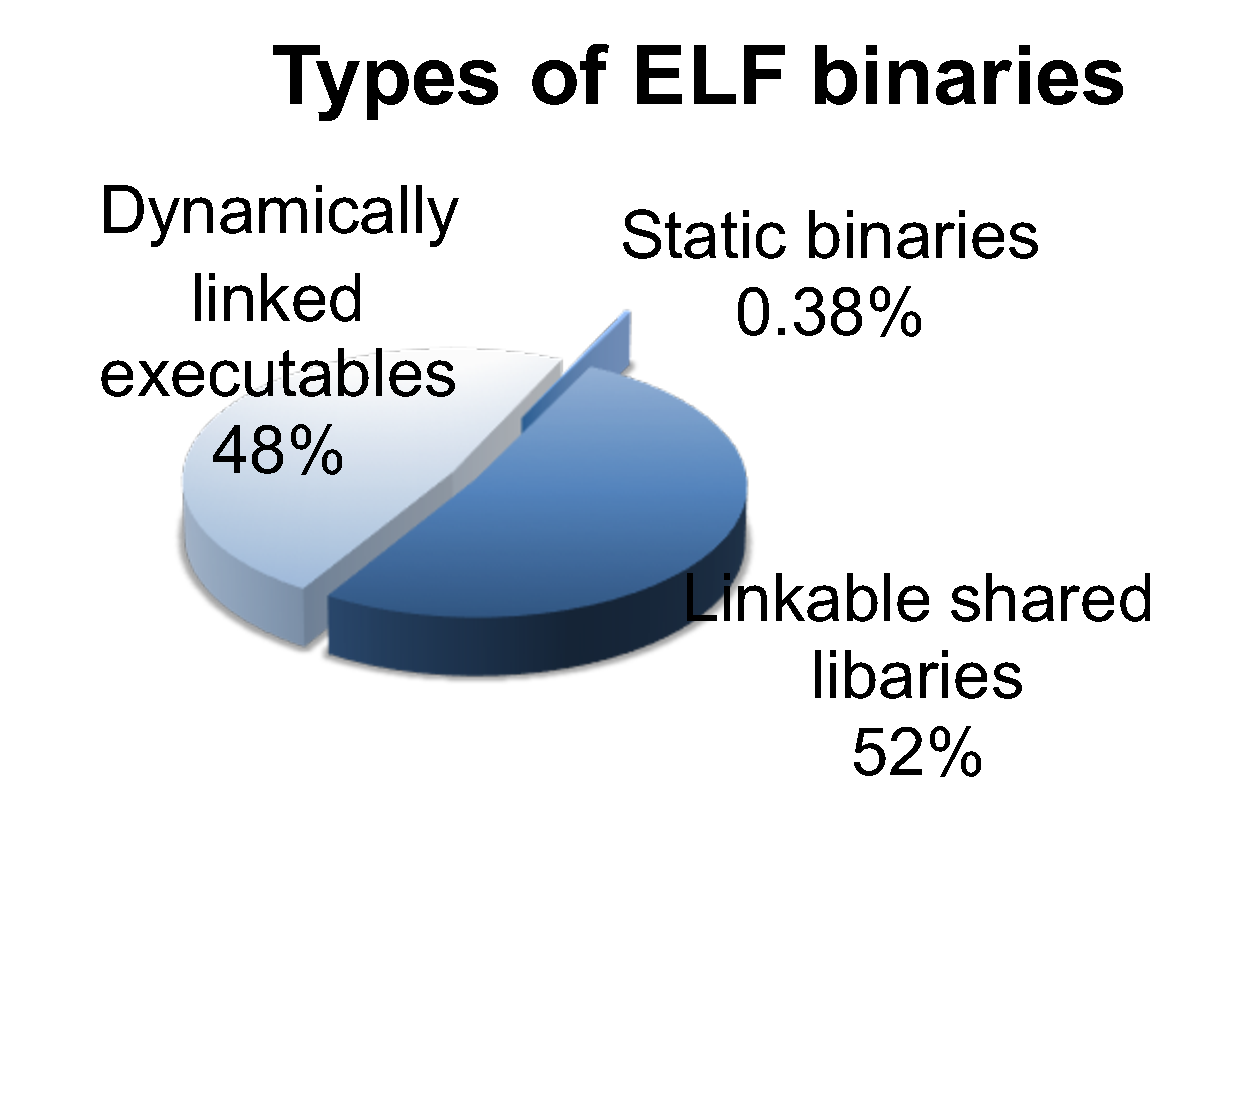
\includegraphics[width=2.4in]{elf-binary-type.pdf}
\vspace{-0.5in}
\footnotesize
\caption{Percentage of ELF binaries and applications written in interpreted languages among all executables in the \osdist{} repository, categorized by interpreters. ELF binaries include static binaries, shared libraries and dynamically-linked executables. Interpreters are detected by {\em shebangs} of the files. Higher is more important.}
\label{fig:syspop:executable-type}
\end{figure}

Our study focuses primarily on ELF binaries, which account for the largest fraction of Linux applications
%which account for the plurality of Linux applications
(Figure~\ref{fig:syspop:executable-type}).
For interpreted languages, such as Python or shell scripts,
we assume that the system call footprint of the interpreter and major supporting libraries over-approximates the expected system call footprint of the applications.
Libraries that are dynamically loaded, such as application modules or
language native interface (e.g.,JNI, Perl XS) are not considered in our study. 
%\fixmedp{Does the analysis handle JNI, Perl XS, or other wrappers for native libraries?  I 
%could imagine the answer being yes if a .so is shipped, but possibly no 
%if it is somehow inlined}

%\fixmedp{Maybe move this up and merge with discussion above}

%% Similarly, there is a distinction between installation and regular use.  Ideally, one might filter applications
%% that were installed but never used, or have a second variant of \usagemetric{} that is weighted by frequency of use.
%% %Although we leave this for future work
%% However, we hasten to note that some infrequently-used applications are nonetheless important to users,
%% and frequency-independent metrics are still important.
%Similarly, there is a distinction between installation and regular use.
%Figure~\ref{fig:package-popularity} shows the trend of package installation statistics for the 500 most commonly installed packages.
%The \byinst{} data may {\it over-approximate} the \usagemetric{} of a package,
%whereas the \byvote{} may {\it under-approximate} important, but infrequently used packages.
%We err on the side of over-approximating \usagemetric{}, using \byinst{}
%weighting where not otherwise specified,
%although we present measurements based on both when appropriate.
%instead under-approximating is a safer strategy to quarantee the compatibility requirements to be fully deliverable.
%In this paper, we present measurements based on both \byinst{} and \byvote{} statisitcs to draw more observations.

%\begin{figure}[t!]
%\vspace{-0.1in}
%\center{
%\includegraphics[width=3.6in]{figures/package-popularity.pdf}
%}
%\footnotesize
%\vspace{-10pt}
%\caption{Package installation statisitics in \osdist{}, for 500 most installed packages managed by the repository. \byinst{} shows installations of packages. \byvote{} shows regularly used packages voted by installations. Higher is more popular.\fixmebj{Change the scale.}}
%\label{fig:package-popularity}
%\end{figure}


\section{Implementation Details}
\label{sec:syspop:framework}

This section provides additional implementation details of our analysis framework. % for mining the API footprint for ELF executables and libraries.

%Analyzing the footprint of an applications requires interpretation of its behavior. As discussed in section~\ref{sec:measure:analysis}, we choose to build our framework by using {\bf static analysis} technique instead of dynamic analysis. The reason is that static analysis can trace potential executions of the applications, regardless of the runtime coverage of the code.

Our analysis is based on disassembling binaries inside each application package, using the standard {\tt objdump} tool.
This approach eliminates the need for source or recompilation, and can handle closed-source binaries.
We implement a simple call-graph analysis to detect system calls reachable from the binary entry point ({\tt e\_entry} in ELF headers). 
%\fixmedp{You do actually parse the elf header for e\_entry, right?}
%In our study, we only count executables during measuring both \usagemetric{} and \compatmetric{}.
We search all binaries, including libraries, for system call instructions ({\tt int \$0x80}, {\tt syscall} or {\tt sysenter}) or calling the {\tt syscall} API of \libc{}.
We find that the majority of binaries --- either shared libraries or executables --- do not directly choose system calls, but 
rather use the GNU C library APIs.
Among 66,275 studied binaries, only 7,259 executables and 2,752 shared libraries issue system calls.

% system calls. Therefore, analyzing the libraries that an executable depends on is necessary for retrieving a complete set of API footprint.


%, to predict its runtime behaviors.
%The framework requires no scanning of the source code, or recompiling of the applications with additional debug symbols.
%Consider the size and complexity of Ubuntu repositories,
%static analysis of ELF binaries is certainly easier to automate, and is able to analyze the applications that are close-sourced.

%To trace the footprint of applications, it require {\em Call-Graph Analysis} to rip off potential control flows that can eventually lead to usage of system API.
%Challenges of analyzing call-graph is a known issues for researchers in many area such as security, robustness, etc.

Our call-graph analysis allows us to only select system calls that are actually used by the application, not all the system calls that appear in \libc{}.
Our analysis takes the following steps:
\begin{compactitem}
\item For a target executable or a library, generate a call graph of internal function usage.
\item For each library function that the executable relies on, identify the code in the library that is reachable from each entry point called by the executable.
%trace coverage of code in the binary, and generate the minimal subset of the library's footprint that the function could actually link to.
\item For each library function that calls another library call, recursively trace the call graph and aggregate the results. 
\end{compactitem}
\vspace{10pt}

Precisely determining all possible call-graphs from static analysis is challenging.
Unlike other tools built on 
call-graphs, such as control flow integrity (CFI), our framework can tolerate the error caused by over-approximating the analysis results.
For instance, 
programs sometimes make function call based on a function pointer passed as an argument by the caller of the function. 
Because the calling target is dynamic, it is difficult to determine at the  call site.
Rather, we track sites where the function pointers are assigned to a register, such as using the {\tt lea} instruction with an address
relative to the current program counter.
%Instead of precisely tracking calling target at the {\tt call} instruction, 
%A function pointer is mostly assigned by {\tt lea} instruction to generate a relative address to the current program counter. 
This is an over-approximation because, rather than trace the data flow, we assuming that a function pointer assigned to a local variable will be called.
This analysis could be more precise if it included a data flow component. 
%\fixmedp{As an aside, this level of data flow analysis shouldn't be that hard, right?  Not  that it matters, except for the thesis/journal version.}

We also hard-code for a few common and problematic patterns.
For instance, we generally assume that the registers that pass a system call number to a system call,
or an opcode to a vectored system call, are not the result of arithmetic in the same function.
We spot checked this assumption, but did not do the data flow analysis to detect this case.

%must trace the register values such as {\tt RAX/EAX} for system call number or {\tt RBX/EBX} for parameter to vectored system calls. 

%Based on {\em Case-by-case study}, we assume no arithmetic but direct assignment of integers is possible when the program is issuing a system call. 

%If our analysis cannot precisely determine whether an API is used, we 
%err on the side of assuming an API is used.

%In the case of a run

%allow slightly enlarge the traced footprint of application, to gain simplicity for complex call-graph analysis corner cases. 
%For the specific run-time scenario of the application that can hard to interpret, we do a {\bf Case-by-Case study} to find out strategy of analyze the footprint practicably.

%  that call-graph analysis is complex for generating the accurate control flow of the run time. Fortunately, unlike other studies that relies on 

%In our study, we specifically call it {\bf Over-approximation}. 


%The following is a few example of using {\bf Over-approximation} and {\bf Case-by-Case study} to simplify call-graph analysis:
%\begin{compactenum}
%\item 
%\item 
%\end{compactenum}

Finally, the last mile of the analysis is to recursively aggregate footprint data. We insert all raw data into a {\tt Postgresql} database, and 
use recursive SQL queries to generate the results. 
To scan through all \packagenum{} packages in the repository, collect the data, and generate the results takes roughly three days.

   




\chapter{Evaluation}
\label{chap:eval}

\subsection{Limitations}
\label{sec:metric:limitations}

%\fixmedp{Make sure we explain these:  the fact that the new metrics cannot distinguish between APIs that are critical to a small population, in that their functionality cannot be provided any other way, because they are new APIs not yet widely adopted, or because they are old APIs that are no longer used or were never used.}

\paragraph{Popularity Contest Dataset.}
The analysis in this paper is limited
by the \osdist{}'s package installer, \osinstaller{},
and their package installation statistics.
Because most packages in \osdist{} are open-source,
our observations on Linux API usage may have a bias toward open-source development patterns.
Commercial applications that are purchased and distributed
through other means are not included in this survey data,
although data from other sources could, in principle, be incorporated
into the analysis if additional data were available.
%the analysis can only be conducted manually,
%thus making it really hard to collect large amounts of samples.

We assume that the package installation statistics provided by \osdist{} are representative.
%The \osdist{} repository hosts \packagenum{} packages that contain application executables and libaries. 
The popularity contest dataset is reasonably large (\popsamples{} installations),
but reporting is opt-in.
Moreover,
%\fixmedp{check this para}
%The popularity contest dataset does not correlate 
%package installations, only shows how often each package is installed.
%Thus, we assume the installation of every package
%as an independent event, unless \osinstaller{} identifies the dependency otherwise.
the data does not show how often these packages
are actually used, only how often they are installed.
Finally, this data set does not include sufficient historical data
to compare changes to the API usage over time.


%% Another limitation of using
%% the package installation statistics
%% is that the statistics only show
%% the installation count of each package,
%% but no details about which packages each installation contains or
%% relative preferences among packages.
%% Therefore, our study must 




%% dp: This is covered elsehwere
%The usage statistics collected in this paper generate
%convincing observations and measurements for Linux-compatible platforms,
%due to the large-scale analysis of software packages in the \osdist{} repository.
%Although our analysis does not require source code,
%our resulting dataset is mostly focused on open-source applications.
%Only very few applications in the \osdist{} repositories are close-source,
%such as the Nvidia driver utilities.
%Our analysis only requires application binaries, and our resulting dataset covers 
%both open-source and closed-source applications. \fixmedp{Right?  Double check that do include some closed binaries}
%Because we focus on \osdist{} applications, and most are open-source (xx\% \fixmetsai{Need to find this number, it's not hard.}),
%the data may be biased toward open-source applications. 
%As a result, our observations on Linux API usage are largely biased toward open-source applications.
%Because the repositories for close-source applications
%are more scattered
%(even though they can be downloaded by \osinstaller{} if manually configured),
%it is hard to collect large amount samples about them.

%% Our study is focused on applications managed by \osinstaller{},
%% which are mostly open-source
%% (even though our approach requires no source code for analysis).

\paragraph{Static Analysis.}
Because our study only analyzes pre-compiled binaries, some compile-time customizations may be missed.
Applications that are already ported using macro like {\tt \#ifdef LINUX} will be considered dependent to Linux-specific APIs,
even though the application can be re-compiled for other systems.
Our static analysis tool only identifies 
whether an API is potentially used,
not how frequently the API is used during the execution.
Thus, it is not sufficient to draw inferences about performance.

%This study is only sufficient to draw conclusions or insight about compatibility, not about any impact on performance.
%The static analysis on application binaries only tells
%Also the package installation statistics provide no information
%about how often a package is used.
%This study cannot provide evidence for whether any APIs may dominate
%execution time.


%\note{Move this here}
We assume that, once a given API (e.g., {\tt write}) is supported and works for a reasonable sample of applications,
handling missed edge cases should be straightforward engineering that is unlikely to invalidate the experimental results of the project.
That said, in cases where an input can yield significantly different behavior, e.g.,
the path given to {\tt open},
we measure the \usagemetric{} of these arguments.
Verifying bug-for-bug compatibility generally requires techniques largely orthogonal to the ones used in this study,
and thus this is beyond the scope of this work.

We do not do inter-procedural data-flow analysis.  As a result,
we were unable to identify system call numbers for 2,454 call sites (4\% of the
relevant call sites)
across all binaries in the repository.  As a result,
some system call usage values may be underestimated, and may go up 
with a more sophisticated static analysis.


%% The package installation statistics provided by \osdist{}
%% show only information about how often packages are ``installed'',
%% not how often packages are ``used''.
%% Our study is based on an over-approximation of the actual package usage:
%% installed packages in any installation contain
%% at least the packages actually used.


\paragraph{Metrics.}
The proposed metrics are intended to be simple numbers for easy comparison.
But this coarseness loses some nuance. 
For instance, our metrics cannot distinguish between
APIs that are critical to a small population, such as those that offer 
functionality that cannot be provided any other way, 
versus APIs that are rarely used because the software is unimportant.
Similarly, these metrics alone cannot differentiate a new API 
that is not yet widely adopted from an old API with declining usage.


%% Although studying historical data may provide more insight about
%% how developer or user behaviors change, our approach requires more historical data to make any conclusions.
%% The installation statistics contain no version information,
%% so it is insufficient to determine the adoption time of any application changes.
%% For packages, \osinstaller{} only keeps the latest version of each package in each maintained snapshot.
%% The only way to backtrace all historical versions of a package
%% is to pull from a version-control repository maintained by the package developers, which may not always exist.

\section{Linux Systems and Emulation Layers}

This section uses \compatmetric{} to evaluate systems or emulation layers with partial Linux compatibility.
We also evaluate several \libc{} variants for their degree of completeness against the APIs exported by \glibc{} 2.21.

\subsection{\CompatMetric{} of Linux Systems}

\begin{table}[t]
\centering
\small
\begin{tabular}{m{0.8in}>{\centering}m{1in}>{\raggedright\arraybackslash\footnotesize}m{3.2in}>{\raggedleft\arraybackslash}m{0.8in}}
\toprule
Systems & \# & Suggested APIs to add & W.Comp. \\
\midrule
\addlinespace
UML \kernelversion{} & 284 & {\tt name\_to\_handle\_at}, {\tt iopl}, {\tt ioperm}, {\tt perf\_event\_open} & 93.1\% \\
\addlinespace
\hline
\addlinespace
L4Linux 4.3 & 286 & {\tt quotactl}, {\tt migrate\_pages}, {\tt kexec\_load} & 99.3\% \\
\addlinespace
\hline
\addlinespace
FreeBSD-emu 10.2 & 225 & {\tt inotify}*, {\tt splice}, {\tt umount2}, {\tt timerfd}* & 62.3\% \\
\addlinespace
\hline
\addlinespace
Graphene  & 143 & {\tt sched\_setscheduler}, {\tt sched\_setparam} & 0.42\% \\
Graphene\textsuperscript{\P} & 145 & {\tt statfs}, {\tt utimes}, {\tt getxattr}, {\tt fallocate}, {\tt eventfd2} & 21.1\% \\
\end{tabular}
\caption{\Compatmetric{} of several Linux systems or emulation layers. For each system, we manually identify the number of supported system calls (``\#''), and calculate the \compatmetric{} (``W.Comp.'') . Based on \usagemetric{}, we suggest the most important APIs to add.
(*: system call family.
\P: Graphene after adding two more system calls.) }
\label{tab:linux-compat}
\end{table}

To evaluate the \compatmetric{} of Linux systems or emulation layers,
the prerequisite is to identify the supported APIs of the target systems.
Due to the complexity of Linux APIs and system implementation,
it is hard to automate the process of identification.
However, OS developers are mostly able to maintain such a list based on the internal knowledge. 

We evaluate the \compatmetric{} of four Linux-compatible systems or emulation layers:
User-Mode-Linux~\citep{user-mode-linux}, L4Linux~\citep{hartig97mu}, FreeBSD emulation layer~\citep{freebsd-emu}, and Graphene library OS~\citep{tsai14graphene}.
For each system, we explore techniques
to help identifying the supported system calls,
based on how the system is built.
For example, User-Mode-Linux and L4Linux
are built by modifying the Linux source code,
or adding a new architecture to Linux.
These systems will define architecture-specific system call tables,
and reimplement {\tt sys\_*} functions in the Linux source
that are originally aliases to {\tt sys\_ni\_syscall}
(a function that returns {\tt -ENOSYS}). 
Other systems, like FreeBSD and Graphene,
are built from scratch,
and often maintain their own system call table structures,
where unsupported systems calls
are redirected to dummy callbacks.

%Because the evaluation is simply a proof-of-the-concept,
%we count only system calls,
%omitting other APIs such as vectored system calls and pseudo-files. 

Table~\ref{tab:linux-compat} shows \compatmetric{},
considering only system calls.
The results also identify the most important system calls
that the developers should consider adding. 
User-Mode-Linux and L4Linux both have a \compatmetric{} over 90\%,
with more than 280 system calls implemented.
FreeBSD's  \compatmetric{} is  62.3\% because it is missing some less
important system calls
such as {\tt inotify\_init} and {\tt timerfd\_create}.
Graphene's \compatmetric{} is only 0.42\%.
We observe that the primary culprit is 
scheduling control; by adding two scheduling system calls,
Graphene's \compatmetric{} would be 21.1\%.

\subsection{\CompatMetric{} of \Libc{}}

\begin{table}[t]
\center{
\setlength{\tabcolsep}{1pt}
\small
\begin{tabular}{m{0.7in}>{\centering}m{0.4in}>{\raggedright\arraybackslash\footnotesize}m{1.1in}>{\raggedleft\arraybackslash}m{0.45in}>{\raggedleft\arraybackslash}m{0.55in}}
\toprule
\Libc{} variants & \# & Unsupported (samples) & {\footnotesize W.Comp.} & {\footnotesize W.Comp.} {\scriptsize (normalized)} \\
\midrule
\addlinespace
eglibc 2.19 & 2198 & None & 100\% & 100\% \\
\addlinespace
\hline
\addlinespace
uClibc 0.9.33 & 1867 & {\tt \_\_uflow}, {\tt \_\_overflow}  & 1.1\% & 41.9\% \\
\addlinespace
\hline
\addlinespace
musl 1.1.14 & 1890 & {\tt secure\_getenv}, {\tt random\_r} & 1.1\% & 43.2\% \\
\addlinespace
\hline
\addlinespace
dietlibc 0.33 & 962 & {\tt memalign}, {\tt stpcpy}, {\tt \_\_cxa\_finalize}  & 0\% & 0\% \\
\end{tabular}
}
\caption{\Compatmetric{} of \libc{} variants. For each variant, we calculate \compatmetric{} based on symbols directly retrieved from the binaries,
and the symbols after reversing variant-specific replacement (e.g.,{\tt printf} becomes {\tt \_\_printf\_chk}).}
\label{tab:libc-compat}
\end{table}

This study also uses \compatmetric{} to evaluate the compatibility of several \libc{} variants --- eglibc~\citep{eglibc}, uClibc~\citep{uclibc}, musl~\citep{musl} and dietlibc~\citep{dietlibc} --- against \glibc{},
listed in Table~\ref{tab:libc-compat}.
We observe that, if simply matching exported API symbols, only eglibc is directly compatible to \glibc{}.
Both uClibc and musl have a low \compatmetric{}, because \glibc{}'s headers replace a number of APIs with safer variants at compile time, using macros.
For example, \glibc{} replaces {\tt printf} with {\tt \_\_printf\_chk}, which performs an additional check for stack overflow.
%Because these new APIs often have the same interface as the old ones,
%we assume other \libc{} variants can easily
%reverse the API replacement during symbol resolution.
After normalizing for this compile-time API replacement, both uClibc and musl are at over 40\% \compatmetric{}.
In contrast, dietlibc is still not compatible with most binaries linked against \glibc{} --- if no other approach is taken to improve its compatibility.
The reason of low \compatmetric{} is that dietlibc does not implement many ubiquitously used \glibc{} APIs such as {\tt memalign} (used by 8887 packages) and {\tt \_\_cxa\_finalize} (used by 7443 packages).

\section{Summary}
\label{sec:graphene:summary}

The \graphene{} design is centered around
building a para-virtualized layer, which can reuse the OS components for reproducing Linux system interfaces.
%instead of building arbitrary compatibility layers for reproducing the system interface.
%constantly porting the significant  of the existing system interface.
%In \graphene{}, 
\graphene{} defines a host ABI, as a new boundary between the OS and user space.
The host ABI is simple enough to port (containing \palcalls{} functions),
and exports sufficient functionality for virtualizing a primary part of the system API components.
A library OS is built upon the host ABI,
and implements \graphenesyscalls{} Linux system calls to reuse unmodified Linux applications.
\graphene{} decouples the development for a compatibility layer,
from host-specific challenges to building OS features, and isolating applications from other malicious tenants.



%\sysname{} extends library OS designs 
%to include multi-process APIs required by common applications, such as a shell or 
%web server.
%\sysname{} demonstrates efficient, selective
%coordination of shared state across multiple library OS 
%instances---maintaining host independence.
%%simplifying security sandboxing of otherwise unwieldy OS features.
%Applications on \sysname{} enjoy both 
%strong security isolation with acceptable performance and low memory overheads.
%% from unrelated programs 
%%and seamless shared namespaces 
%%among a group of coordinating guests.
%%% Although this paper focuses on distributed coordination
%%% to facilitate the efficiency benefits,
%%% expect our experiences with distributed coordination 
%%% may also be particularly relevant to highly scalable OS designs, 
%%% which avoid the bottlenecks of shared OS data structures~\cite{baumann09barrelfish, song11eurosys}.
%%Graphene's overheads are acceptable and the memory 
%%footprint is substantially lower than a VM.



%% , which could benefit from the reduced memory footprint
%% in a cloud 

%% by introducing a novel design for  coordination APIs. 
%% to a new OS (Linux),
%% new classes of applications,
%% and introduces a
%% %an alternative design point for storage virtualization.
%% Our results further demonstrate the feasibility of the library OS model.
%% % generally,
%% Applications on Graphene enjoy both 
%% strong security isolation from unrelated programs 
%% and seamless shared namespaces 
%% among a group of coordinating guests.
%% Although we explore this concept in a library OS,
%% we expect the namespace coordination framework 
%% could also be adapted to limit the attack surface area between
%% processes in a traditional OS.
%% We expect these experiences with distributed coordination 
%% may also be particularly relevant to highly scalable OS designs, 
%% which avoid the bottlenecks of shared OS data structures~\cite{baumann09barrelfish}.
%and specifically of content-addressable storage as the primary virtual storage abstraction.
%%% This work opens up a number of interesting questions for future work, 
%%% including studying opportunities for low-level storage optimization within the CAS server,
%%% making CAS the root file system,
%%% eliminating storage management in the host kernel, and 
%%% investigating the impact of frequent migration among devices.

\begin{comment}
Enabling legacy applications in a restricted environment,
such as \picoprocs{} or enclaves,
requires extra effort for mitigating the limitations of platforms,
in order to support typical OS personalities.
\graphene{}, as described in this chapter, extends the existing \libos{} designs
from isolating single-process or unshared abstractions
to include multi-process APIs required by many UNIX applications,
such as servers or shell scripts.
The challenge that \graphene{} primarily overcomes
is the requirement for coordinating shared states across multiple \picoprocs{},
to provides a collaborative, unified OS view.
Essentially, \graphene{} implements all shared, multi-process abstractions
and OS states
based on coordination over host-provided, pipe-like RPC streams.
The RPC-based, distributed OS implementation enables multi-process support in \graphene{}, with minimal extension to the host interface,
and a sweet-spot for enforcing inter-application security isolation,
by simply sandboxing the RPC streams.
Such a model largely reduces the complexity of
enforcing security isolation
on idiosyncratic multi-process abstractions
and shared states.
Because the corporative nature of \picoprocs{} in \graphene{},
an application can even dynamically impose sandboxing on one of its processes,
to reflect per-process, variable security policies.
\end{comment}

\begin{comment}
In principle, we attempt to use \graphene{} to justify the platform independence
of the \libos{} design,
without sacrificing its qualitative benefits,
such as isolating mutually-untrusting applications
and a narrow attack surface to kernels.
\graphene{} implements a considerable number of common Linux system calls,
to support popular, modern applications
such as Apache web server, GNU Make, OpenJDK \java{} VM and the Python runtime.
\graphene{} translates the high-level system APIs used by applications
to a host ABI
inherited and extended from a previous Windows-compatible \libos{}~\cite{porter11drawbridge}.
In addition, we port the \pal{} (Platform Adaption Layer) of \graphene{}
to various platforms,
including FreeBSD, OSX, Windows, and even a more restricted environment, the \intel{} \sgx{} enclaves.
In particular, \graphene{} being ported to \intel{} \sgx{}
(\graphenesgx{})
can isolate applications --- either single-process or multi-process
--- on a host where neither the operating system nor the hardware (except the CPU package)
is trusted by the applications. 
Overall, \graphene{} shows that,
by simply porting the reasonably sized host ABI
to a new platform,
a whole large spectrum of legacy applications tested on the previous platforms
can be activated all together.
\end{comment}


\chapter{A Study of System APIs}
\label{chap:study}
\section{Linux API Study}
\label{sec:syspop:study}

%\note{about 3 pages, include graphs}
%\note{try to break the page here so the whole observation can start on a new page}

%This section presents measurements of API usage,
%as well as several trends in how APIs are used. Of particular note is that
%the OS interface required by essentially all applications is 
%%the total OS interface that essentially all applications require is
%substantially larger than the roughly 300 Linux system calls---the required interface
%also includes several vectored system call operations, such as {\tt ioctl}, and special filesystem interfaces like {\tt /sys} and {\tt /proc}.
%We also note that a number of system calls and other APIs are so rarely used that they can be deprecated with little disruption or effort.
%
%This section first examines the use of system calls in Linux applications.
%Section~\ref{sec:observation:hello} analyzes the most efficient path to add system calls
%to a prototype, outlining a path from the minimal footprint for ``hello world'', 
%up through the most demanding application (qemu), maximizing the number
%of supported applications at each step.
%Section~\ref{sec:observation:vector} analyzes the importance of operations
%under vectored system calls, such as {\tt ioctl}.
%Section~\ref{sec:observation:pseudo} evaluates the \usagemetric{} of 
%pseudo-files, such as those under {\tt /proc}.
%Finally, Section~\ref{sec:observation:libc}
%examines current usage patterns for \libc{}.
%Throughout the section, we identify several points at which APIs could be gainfully
%restricted, removed, or refactored,
%as well as identifying points where unexpected APIs can be essential to performance or
%functionality.
%We highlight key insights and recommendations in boxes.

%% \rev{Explain the structure.}{In the following subsections,
%% we will discuss our findings on the API usage of different interface types,
%% followed by %boxed take-aways our quick tips (in double-framed boxes)
%% the lessons or insights in boxes.} 
%% \fixmedp{If a reviewer asked for a structure, I expect they want to know something like:
%% We first present system calls, then ioctls,
%% then pseudo file systems, etc.  In other words, what is the organizing principle for 
%% the following sub-sections?  Not that we discuss and then have a box} 

%\subsection{\usagemetric{} of Linux System Calls}
\subsection{System calls}
\label{sec:syspop:study:syscall}

%We begin by looking at the \usagemetric{} of each system call, 
%ordered by total application installations and regularly used applications 
%in order to answer the following questions:
%\begin{compactitem}
%\item Which system calls are the most important to support when implementing a new system,
%or have high costs to replace, if desired?
%%1) do we definitely need to support any of the surveyed systems?
%%2) are used by at least one frequently used application on the surveyed systems?
%\item Which system calls are very rarely used and candidates for deprecation?
%\item Which system calls are not supported by the OS, but still attempted by applications?
%\end{compactitem}
%\vspace{10pt}

There are \syscallnum{} system calls defined in \osarch{} Linux \kernelversion{} (as listed in {\tt unistd.h}). 
Figure~\ref{fig:syscall-popularity-trend} shows the 
distribution of system calls by importance.
The Figure is ordered by most important (at 100\%) to least important (around 0\%)---similar
to inverted CDF.
The figure highlights several points of interest on this line.

%The trends \byinst{} are useful to answer questions about supporting complete installations, 
%while the trends \byvote{} are useful to answer questions about supporting most popular 
%applications on most of the systems.
Over two-thirds ({\em 224 of \syscallnum{}}) 
of system calls on Linux are indispensable:
required by 
at least one application on every installation.
%only a little 
%over one-thirds ({\em 121 of \syscallnum{}}) of system calls are required 
%by at least one regularly used application (\byvote{}).
%\fixmedp{Would be nice to have more to say here, like filling out weighted compliance and the number of packages}
Among the rest, 33 system calls are important on more than ten percent of the installations.
44 system calls have very low \usagemetric{}:
less than ten percent of the installations include at least one application
that uses these system calls.
%Moreover, less than 10\% of the systems require 43 system calls.
%and 58 system calls are regularly used on less than 10\% of the systems (\byvote{}).
%For instance, {\tt timer\_delete}, {\tt timer\_create} and {\tt timer\_settime} are used by 
%at least one application on all the systems, however, the applications using these 
%system calls are regularly used only on 17\% of the systems. 
%Another system call 
%{\tt tkill} used by {\tt strace} installed ubiquitously on all systems 
%is used regularly only on 3\% of the systems. So, even if the installation statistics imply that 
%{\tt tkill} needs to be supported to support at least one of the machines,
%only 3\% of those machines regularly use that system call.

Our study also shows the contributors
to an API's importance. %\usagemetric{}.
For instance, Table~\ref{tab:syspop:wrapped} lists system calls that are
only called by one or two particular libraries
(e.g., \libc{}).
These system calls are wrapped by library APIs,
so applications depend on them only because the libraries do.
To eliminate the usage of these system calls,
developers only have to pay minimum efforts to re-implement the wrappers in libraries.

\begin{figure}[t]
\centering
\includegraphics[width=\textwidth]{syscall-popularity-all-by-inst.pdf}
\caption[N-most important system calls in Linux.]
{The trend of \usagemetric{} as N-most important system calls among total \syscallnum{} system calls of \osversion{} with Linux kernel \kernelversion{}. .
Higher is more important; 100\% indicates all installations include software that make the system call.}
\label{fig:syscall-popularity-trend}
\end{figure}

%\callout{It is easy to support regularly used parts of an installation than complete installations of the surveyed systems.} 

Among the 44 system calls with a \usagemetric{} above zero but less than ten percent,
some are cases where a more popular alternative is available.
%developers appear more motivated by 
%portability than security.
%, the bottom 20 non-zero are listed in Table~\ref{tab:syscall-popularity-bottom}, along with the packages that use these interfaces.
%%11 of the bottom 20 system calls are Linux-specific.
%%This shows that portability to other Unix variants
%%has a significant effect on adoption.
%%bP: These conclusions cannot be made with weighted importance.
For instance, Linux supports both POSIX and System V message queues.
The five APIs for POSIX message queues have a lower
\usagemetric{} than System V message queues.
We believe this is attributable to System V message queues %provide a better designed interface, they
being more portable to other UNIX systems.
%they are not adopted by most popular applications.}
Similarly, we observed that {\tt epoll\_wait} (100\%) has a higher \usagemetric{} than {\tt epoll\_pwait} (3\%),
even though {\tt epoll\_pwait} is commonly considered more robust
for the same purpose---waiting on file descriptor events.
Table~\ref{tab:dominated} lists
system calls used by only one or two packages---generally special-purpose utilities,
such as {\tt kexec\_load}, which is used by {\tt kexec-tools}).
%,These system calls are mostly used by special-purpose utilities (e.g., 
%and generally address  because their semantics are not friendly enough.

\begin{table}[t!b!]
  \centering
  \small
  \begin{tabular}{>{\footnotesize\raggedright\arraybackslash}p{1.45in} >{\raggedleft\arraybackslash}p{0.25in}>{\raggedright\arraybackslash}p{1.15in}}
\toprule
{\bf System Calls} & {\bf Imp.} & {\bf Packages}\\
\midrule
{\tt clock\_settime}, {\tt iopl}, {\tt ioperm},  {\tt signalfd4}  & 100\% & libc \\
{\tt mbind}             & 36.0\% & libnuma, libopenblasp \\
{\tt addkey}            & 27.2\% & libkeyutils \\
{\tt keyctl}            & 27.2\% & pam\_keyutil, libkeyutils \\
{\tt requestkey}        & 14.4\% & libkeyutils \\
{\tt preadv}, {\tt pwritev}   & 11.7\% & libc \\
    \end{tabular}%
   \caption{System calls which are only directly used by particular libraries, and their \usagemetric{} (``Imp.''). Only system calls with \usagemetric{} larger than ten percent are shown.
These system calls are wrapped by library APIs,
thus they are easy to deprecate by modifying the libraries.  
}
  \label{tab:wrapped}%
\end{table}%

\begin{table}[t!b!]
\centering
\small
\begin{tabular}{>{\palign[\footnotesize]{l}}p{2.9in} >{\palign{r}}p{1.1in}>{\palign{l}}p{2in}}
\toprule
{\bf System Calls} & {\bf \UsageMetric{}} & {\bf Used Packages}\\
\midrule
{\tt seccomp}, {\tt sched\_setattr}, {\tt sched\_getattr}  & 1\% & coop-computing-tools \\
\hline
{\tt kexec\_load} & 1\% & kexec-tools \\
\hline
{\tt clock\_adjtime} & 4\% & systemd \\
\hline
{\tt renameat2} & 4\% & systemd, coop-computing-tools \\
\hline
{\tt mq\_timedsend}, {\tt mq\_getsetattr} & 1\% & qemu-user \\
\hline
{\tt io\_getevent} & 1\% & ioping, zfs-fuse \\
\hline
{\tt getcpu} & 4\% & valgrind, rt-tests \\
\hline
\end{tabular}%
\caption[System call usage dominated by particular package(s)]
{System calls with usage dominated by particular package(s), and their \usagemetric{}. This table excludes system calls that are officially retired.}
\label{tab:dominated}%
\end{table}%


In some cases, system calls are effectively offloaded to a file in {\tt /proc} or {\tt /sys}.
For instance, some of the information that was formerly available via 
{\tt query\_module} can be obtained from {\tt /proc/modules}, {\tt /proc/kallsyms} 
and the files under the directory {\tt /sys/module}. Similarly, the information that can be obtained from the {\tt sysfs} system call
is now available in {\tt /proc/filesystems}.

%We found five  API that have very low 
%compared to the System V message queue API.

We also found five system calls {\tt uselib}, {\tt nfsservctl}, {\tt afs\_syscall}, {\tt vserver} and {\tt security} system calls that are officially retired, but still have a low, but non-zero, \usagemetric{}. 
For instance {\tt nfsservctl} is removed from Linux kernel 3.1 but
still has \usagemetric{} of seven percent,  %\fixmedp{Do we have some examples of apps that use it?}
because it is tried by NFS utilities such as {\tt exportfs}.
These utilities still attempt the old calls for backward-compatibility with older kernels.
%Application maintainers of packages using these retired system calls need to be notified to port their applications to support latest kernel.


%\callout{System developers can use our framework to actively notify relevant package maintainers while retiring system calls.} 
%\callout{Among 43 least-used system calls, some are replaceable
%by alternatives with higher \usagemetric{};
%5 are officially retired but still tried by few applications.
%System developers could use this data to identify relevant applications,
%accelerating replacement of these system calls.}




\begin{table}[t!b!]
\centering
\small
\begin{tabular}{>{\palign[\footnotesize]{l}}p{.5\textwidth} >{\palign{l}}p{.45\textwidth}}
\toprule
\textbf{Unused System Calls} & \textbf{Reason for Disuse}\\
\midrule
{\footnotesize
{\tt set\_thread\_area}, {\tt tuxcall}, {\tt create\_module}, and 7 more. } & Officially retired.\\
\hline
{\tt sysfs} & replaced by {\tt /proc/filesystems}.\\
\hline
{\tt rt\_tgsigqueueinfo}, {\tt get\_robust\_list} & Unused by applications.\\
\hline
{\tt remap\_file\_pages} & No non-sequential ordered mapping; repeated calls to mmap preferred.\\
\hline
{\tt mq\_notify} & Unused: Asynchronous message delivery.\\
\hline
{\tt lookup\_dcookie} & Unused: for profiling.\\
\hline
{\tt restart\_syscall} & Transparent to applications.\\
\hline
{\tt move\_pages} & Unused: for NUMA usage. \\
\hline
\end{tabular}%
\caption{Unused system calls and explanation for disuse.}
\label{tab:syspop:unused}%
\end{table}%



%On the other end of the spectrum, 

In total, 18 of \syscallnum{} system calls in Linux \kernelversion{} are not used by any application in the \osdist{} repository. We list these system calls in Table~\ref{tab:syspop:unused}.
In addition to the issues discussed above,
Ten of these system calls do not have an entry point, but are still defined in the Linux headers.
%\fixmedp{Why are they in the count then?  do you mean 320 defined system call numbers}
%Similarly, we analyze the 21 system calls with 0 \usagemetric{} as shown in 
%Table~\ref{tab:unused}. 
%{\tt sysfs} is replaced by alternate interface {\tt /proc/file\linebreak[0]systems}.
%%On the other hand, even though {\tt remap\_file\_pages} system call was added to map pages of a file into memory in a non-sequential order since Linux version 2.6 (in 2003), no application is actually using it. This indicates that either no application is mapping pages in non-sequential order or applications are repeatedly using the more popular generic system call like {\tt mmap}.
%Similarly, {\tt mq\_notify} system call for receiving asynchronous notification about new messages in message queue is not used, because \usagemetric{} of message queue interfaces is less than 5\% in the first place and applications using message queue do not use asynchronous communication.
Five of the unused system calls such as {\tt rt\_tgsig\linebreak[0]queueinfo}, {\tt get\_robust\_list}, {\tt remap\_\linebreak[0]file\_pages}, {\tt mq\_notify}, {\tt lookup\_dcookie} provide an interface that is not used by the applications. These system calls can be potential candidates for deprecation.
However, even though {\tt restart\_\linebreak[0]syscall} is not used by any application, it is internally used by the kernel. % transparent to userspace.
%Finally, 4 NUMA related system calls are not used 
%\rev{rewrite}{because none of our samples is written to be NUMA-aware}.
%\fixmetsai{Check if libnuma uses these system calls.}

%\callout{In addition to ten already retired system calls, we found seven other candidate system calls for deprecation or in need of more exposure to developers.}

\begin{comment}
\begin{table}[t]
\center{
\footnotesize
\begin{tabular}{m{0.45\linewidth}m{0.45\linewidth}}
\hline
Syscalls & Packages\\
\hline
process\_vm\_writev & coop-computing-tools, care, proot, stress-ng \\
vserver & util-vserver\\
syncfs & ceph-test, ploop, ruby-passenger, ceph\\
io\_getevents & ioping, zfs-fuse\\
uselib & mupdf, mupdf-tools\\
afs\_syscall & openafs-fileserver, openafs-kpasswd, openafs-krb5, openafs-client, openafs-dbserver\\
kexec\_load & kexec-tools\\
mq\_getsetattr, mq\_timedsend & qemu-user, qemu-user-static\\
vmsplice & criu, qemu-user-static, fio, stress-ng, qemu-user\\
timer\_gettime & ben, galax-extra, libocamlnet-ocaml-bin, ocsigenserver, galax, approx, qemu-user-static, galaxd, matita, cduce, qemu-user, turnserver, stress-ng\\
timerfd\_gettime & ben, approx, libocamlnet-ocaml-bin, ocsigenserver, openclonk, matita, galax, galaxd, qemu-user-static, galax-extra, cduce, qemu-user\\
eventfd & blktap-utils, julia, nodejs\\
semtimedop & tgt, dahdi, gtk-gnutella, prayer, libopenni-sensor-primesense0, libopenni-sensor-pointclouds0\\
timer\_getoverrun & emacs24-lucid, emacs24, qemu-user-static, qemu-user, emacs24-nox, rt-tests, reconserver, miredo\\
mq\_timedreceive & qemu-user-static, nilfs-tools, xjadeo, rt-tests, qemu-user\\
acct & watchdog, acct, qemu-user-static, qemu-user, scm, atop\\
fanotify\_init, fanotify\_mark & fatrace, fnotifystat, health-check, clamav-daemon\\
open\_by\_handle\_at & qemu-system-mips, qemu-system-misc, qemu-system-sparc, qemu-system-ppc, qemu-system-arm, qemu-system-x86\\
\hline
\end{tabular}
}
\footnotesize
\caption{20 system calls with the lowest \usagemetric{} among 297 used system calls in \osversion{} with Linux Kernel \kernelversion{}, except the ones with \usagemetric{} lower than 0.01\% (considered negligible).}
\label{tab:syscall-popularity-bottom}
\end{table}
\end{comment}

\begin{comment}
There are 43 system calls with low non-zero \usagemetric{} of less than 10\%.
%, the bottom 20 non-zero are listed in Table~\ref{tab:syscall-popularity-bottom}, along with the packages that use these interfaces.
%%11 of the bottom 20 system calls are Linux-specific.
%%This shows that portability to other Unix variants
%%has a significant effect on adoption.
%%bP: These conclusions cannot be made with weighted importance.
We found 5 POSIX message queue API that have very low 
\usagemetric{} compared to the System V message queue API because 
even if POSIX message queues provide a better designed interface, they are less 
widely available. We also found 5 system calls {\tt uselib}, {\tt nfsservctl}, {\tt afs\_syscall}, {\tt vserver} and {\tt security} system calls that are officially retired, and have non-zero albeit negligible \usagemetric{}. 
For instance {\tt nfsservctl} is removed from Linux kernel 3.1 but
still has \usagemetric{} of 7\%. Application maintainers of packages using these retired system calls need to be notified to port their applications to support latest kernel.
Also, we observed that {\tt epoll\_wait} (100\%) has more \usagemetric{} than {\tt epoll\_pwait} (3\%)
even though {\tt epoll\_pwait} is safer to use to wait for a file descriptor to become available.
In some cases, system calls are effectively offloaded to a file in {\tt /proc} or {\tt /sys}.
For instance, some of the information that was formerly available via 
{\tt query\_module} can be obtained from {\tt /proc/modules}, {\tt /proc/kallsyms} 
and the files under the directory {\tt /sys/module}. Also same information obtained from {\tt sysfs} is
also available from {\tt /proc/filesystems}.

\callout{System developers can use our framework to actively notify relevant package maintainers while retiring system calls.} 
\end{comment}

%%% \begin{figure}[H]
%%% \center{
%%% \includegraphics[height=1.1in]{figures/syscall-popularity-top-1.pdf}
%%% \hspace{-0.3in}
%%% \includegraphics[height=1.1in]{figures/syscall-popularity-top-2.pdf}
%%% }

%%% \begin{minipage}[t]{\linewidth}
%%% \scriptsize
%%% \vspace{-0.1in}
%%% \setlength{\parindent}{-0.2in}
%%% \setlength{\leftskip}{0.2in}
%%% {\bf * Top-1:} \hspace{0.1in}(195 system calls) \hspace{0.1in}\usagemetric{} = 1.0000\\
%%% {\tiny\tt
%%% read,write,open,close,stat,polllseek,mmap,brk,rt\_sigprocmask,ioctl,access,pipe,select,shmget,nanosleep,socket,clone,vfork,kill,
%%% etc.
%%% }

%%% \vspace{0.1in}
%%% {\bf * Top-2:} \hspace{0.1in}(8 system calls) \hspace{0.1in}\usagemetric{} = 0.9999\\
%%% {\tiny\tt
%%% reboot,timer\_create,iopl,getitimer,accept4,
%%% etc.
%%% }
%%% \end{minipage}
%%% \footnotesize
%%% \caption{20 groups of system calls with the highest \usagemetric{} among 279 used system calls in \osversion{} (Linux Kernel \kernelversion{})}
%%% \label{fig:syscall-popularity-top}
%%% \end{figure}

%\begin{figure}[H]
%\center{
%\includegraphics[height=1.15in]{figures/syscall-popularity-bottom.pdf}
%}
%\footnotesize
%\caption{20 system calls with the lowest \usagemetric{} among 279 used system calls in \osversion{} (Linux Kernel \kernelversion{}), except the ones with \usagemetric{} lower than 0.0001 (considered negligible).\fixmedp{Convert to table}}
%\label{fig:syscall-popularity-bottom}
%\end{figure}

%\subsection{From ``Hello World'' to Qemu}
%\label{sec:observation:hello}

Figure~\ref{fig:syscall-compatibility} shows the optimal path of adding system calls to a prototype system,
using a simple, greedy strategy of implementing the N-most important APIs, which in turns
maximizes \compatmetric{}.
In other words, the leftmost points on the graph are the most important APIs,
but the y coordinate only increases once enough system calls
are supported that a simple program, such as ``hello world'' can execute. %\fixmedp{Right?}
Similar to a CDF, this line
continues up to 100\% of Ubuntu applications.  The graph highlights several 
points of interest in this curve.

Essentially, one cannot run even the most simple programs without at least 40 system calls.
After this, the number of additional applications one can support by adding another system call increases
steadily until an inflection point at 125 system calls, or supporting extended attributes on files,
where \compatmetric{} jumps to 25\%.
To support roughly half of \osdist{} applications, one must have 145 system calls, and
the curve plateaus around 202 system calls.  
On the most extreme end, qemu's MIPS emulator (on an \osarch{} host) requires 270 system calls~\citep{Bellard05}.
A \compatmetric{} of 100\% implies that
%all Linux system calls
all Linux applications ever used
are supported by the prototype.

\begin{figure}[t]
\centering
\includegraphics[width=.8\textwidth]{syscall-compatibility.pdf}
\caption{Accumulated \compatmetric{} when N top-ranked system calls are implemented in the OS. Higher is more compliant.}
\label{fig:syscall-compatibility}
\end{figure}

\begin{table}[t]
\center{
\begin{tabular}{c>{\footnotesize\raggedright\arraybackslash}m{.5\textwidth}>{\raggedleft}m{.15\textwidth}>{\raggedleft\arraybackslash}m{.15\textwidth}}
\toprule
Stage & {\normalsize Sample System Calls} & \# syscalls & {\footnotesize \CompatMetric{}} \\
\addlinespace
\midrule
I &
{\tt mmap}, {\tt vfork}, {\tt exit}, {\tt read},
{\tt gettid}, {\tt fcntl}, {\tt getcwd}
{\tt sched\_yield}, {\tt kill}, {\tt dup2}
& 40 & 1.12 \% \\
\midrule
II &
{\tt mremap}, {\tt ioctl}, {\tt access}, {\tt socket},
{\tt poll}, {\tt recvmsg}, {\tt dup},
{\tt unlink}, {\tt wait4}, {\tt select}, {\tt chdir}, {\tt pipe}
& +41 (81) & 10.68 \% \\
\midrule
III &
{\tt sigaltstack}, {\tt shutdown}, {\tt symlink},
{\tt alarm}, {\tt listen}, {\tt pread64}, {\tt getxattr}, 
{\tt shmget}, {\tt epoll\_wait},
{\tt chroot}
& +64 (145) & 50.09 \% \\
\midrule
IV &
{\tt flock}, {\tt semget}, {\tt ppoll},
{\tt mount}, {\tt brk}, {\tt pause},
{\tt clock\_gettime}, {\tt getpgid}, {\tt settimeofday},
{\tt capset}
& +57 (202) & 90.61 \% \\
\midrule
V & {\normalsize All remaining} & +70 (272) & 100 \% \\
\bottomrule
\end{tabular}
}
\footnotesize
\caption[Proposed steps of Linux system call implemetation prioritzed by importance]
{Five stages of implementing system calls based on the \usagemetric{} ranking. For each stage, a set of system calls is listed, with the work needed to accomplish (\# of system calls) and the \compatmetric{} that can be reached.}
\label{table:syscall-stage}
\end{table}

Table~\ref{table:syscall-stage} breaks down the recommended development phases by rough categories of required system calls.
We do not provide a complete ordered list here in the interest of brevity, but this list is available as part of our dataset, 
at \projecturl{}.

A goal of \compatmetric{} is to help guide the process of developing new system prototypes.
Section~\ref{sec:observation:syscall} showed that 224 out of \syscallnum{} system calls on \osdist{} have 100\% \usagemetric{}.
In other words, if one of these 224 calls is missing, at least one application on a typical system will not work.
\Compatmetric{}, however, is more forgiving, as
it tries to capture the fraction of a typical installation that could work.
Only 
40 system calls are needed to have \compatmetric{} more than 1\%.
%However, to achieve non-zero \compatmetric{} to \osdist{}, it does not require a system to support all 226 system calls;
%only 
%% The reason of such a gap is that \usagemetric{} is
%% a metric more sensitive to the API usage of individual applications:
%% as long as at least one application in every installation uses
%% a specific API, its \usagemetric{} will be 100\%.
%% \compatmetric{} is a metric made relatively relaxed:
%% this metric evaluates the expected fraction of any installation that can be supported,
%% to provide meaningful measurements

%\callout{It takes the most effort to support first and last 10\%
%of any installation (0--10\% and 90--100\% \compatmetric{}).
%The gain in functionality is precipitous when adding the 81st--202nd system calls.}

For simplicity, Table~\ref{table:syscall-stage}
only includes system calls, % \compatmetric{} based on system ,
but one can construct a similar path including other APIs, % the metric also considers other APIs,
such as vectored system calls, pseudo-files and library APIs.
For example, developers need not implement every operation of
{\tt ioctl}, {\tt fcntl} and {\tt prctl}
during the early stage of developing a system prototype.
%\fixmedp{Would it make sense to do this after the ioctls and files are covered, and include important ioctls and files?  Also, check my rewrite}

%\fixmedp{This callout is not really justified by the text  I took the point to be that the right 132 and 202 system calls are ``sweet spots'' on the path to maturity.}

\subsection{Vectored System Calls}
\label{sec:syspop:study:vector}

%\fixmedp{I think RD is right: can we give more landscape of what the long tail of vectored calls are for?  Why do they exist?}

Some system calls, such as {\tt ioctl}, {\tt fcntl},
and {\tt prctl}, essentially export a secondary system call table, 
using the first argument as an operation code.
These {\it vectored} system calls significantly expand the system API, 
dramatically increasing the effort to realize full API compatibility.
%and essentially make it harder to implement a compatibility layer.
It is also difficult to enforce robust security policies on these interfaces,
as the arguments to each operation are highly variable.
%\fixmedp{Can we comment on what, say SELinux or AppArmor actually do with ioctl?}


The main expansion is from {\tt ioctl}.
Linux defines 635 operation codes, and 
Linux kernel modules and drivers can define additional operations.
In the case of {\tt ioctl}, we obverse that there are 52 operations with the 100\% \usagemetric{} (Figure~\ref{fig:syspop:opcode-popularity}),
each of which are as important as the 226 most important system calls.
Of these 52 operations,  47 are frequently used operations for TTY console (e.g., {\tt TCGETS}) or generic operations on IO devices (e.g., {\tt FIONREAD}).

%A narrow vectored system call like {\tt fcntl} has eighteen operations in , and {\tt prctl} has 44 operations so far.
%A wider vectored system call like 
%which are further 



On the narrow end, {\tt fcntl} and {\tt prctl} have 18 and 44 operations, respectively, in Linux kernel \kernelversion{}.
Unlike {\tt ioctl}, {\tt fcntl} and {\tt prctl} are not extensible by modules or drivers,
and their operations tend to have higher \usagemetric{} (Figure~\ref{fig:syspop:opcode-popularity}).
For {\tt fcntl}, eleven out of eighteen {\tt fcntl} operations in Linux \kernelversion{} have \usagemetric{} at around 100\%.
For {\tt prctl}, only nine out of 44 operations have \usagemetric{} around 100\%,
and only eighteen has \usagemetric{} larger than 20\%.
%Because of the more equally important operations, {\tt fcntl} is a less urgent target for reformation, while {\tt prctl} has plenty of unused or infrequently used read-only operations that can be moved to pseudo-file system interfaces like {\tt /proc}.


Thus, developers of a new system prototype should support these 47 most important {\tt ioctl}
operations, about half of the {\tt fcntl} opcodes, and only 9--20 {\tt prcntl} operations.


%% Although the 47-most important ioctl operations have 100\% \usagemetric{},
%% promoting any of these operations to system calls is not beneficial.
%% Vectored system calls with limited amounts of operation codes
%% are almost equally easy to secure and maintain
%% as normal system calls.
%% However the disruptiveness of removing these operations codes
%% is unbearable for applications. 

%% However, knowing the most important operations for vectored system calls,
%% developers of new system prototypes can choose to
%% implement only part of these vectored system calls to obtain significant improvement on \compatmetric{}.
%% %For instance, Graphene library OS~\citep{tsai14graphene} only implements {\tt FIONREAD} of {\tt ioctl} to satisfy the most common usage in applications. 

%\callout{In building a prototype system, a relatively small set of operations
%in vectored system calls are essential.}
%Highly important operations in vectored system calls
%can be implemented first, to achieve better \compatmetric{}
%with partial support of these system calls.}}

%These operations are candidates for promotion to standalone system calls,
%for better usability, more attention for their security, and ease of filtering.  

%\callout{The most ubiquitous vector operations should be upgraded to system calls.}


Compared to system calls, 
{\tt ioctl} has a much longer tail of infrequently used operations.
Out of 635 {\tt ioctl} operation codes defined by modules or drivers hosted in Linux kernel \kernelversion{},
only 188 have \usagemetric{} more than one percent,
and for only 280 we can find usage of the operations in at least one application binary.
Those unused operations are good targets for deprecation, in the interest
of reducing the system attack surface.
%since leaving them around causes the OS open to attacks if any vulnerabilities exist in these APIs.
%\fixmetsai{What can we find out in this long tail?}

%\callout{{\tt ioctl} system call has a very long tail of unused operations, which may create system security risks.}

\begin{figure}[t]
\centering
\includegraphics[width=.48\textwidth]{ioctl-popularity-by-inst.pdf}
\includegraphics[width=.25\textwidth]{fcntl-popularity-by-inst.pdf}
\includegraphics[width=.25\textwidth]{prctl-popularity-by-inst.pdf}
\caption{Ranking of \usagemetric{} among {ioctl}, {\tt fcntl} and {\tt prctl} opcodes.  Higher is more important; 100\% indicates all installations include software that request the operations.}
\label{fig:syspop:opcode-popularity}
\end{figure}


%\fixmedp{If time, it would be nice to investigate these zero cases and make sure no one really uses them}

%\begin{figure}[t]
%\center{
%\includegraphics[width=0.95\linewidth]{figures/fcntl-popularity.pdf}
%}
%\footnotesize
%\caption{Ranking of \usagemetric{} among {\tt fcntl} commands.}
%\label{fig:fcntl-popularity}
%\end{figure}

%\begin{figure}[t]
%\center{
%\includegraphics[width=0.95\linewidth]{figures/prctl-popularity.pdf}
%}
%\footnotesize
%\caption{Ranking of \usagemetric{} among {\tt prctl} codes.}
%\label{fig:prctl-popularity}
%\end{figure}

\subsection{Pseudo-Files and Devices}
\label{sec:syspop:study:pseudo}

In addition to the main system call table, Linux exports many additional APIs through 
pseudo-file systems, such as {\tt /proc}, {\tt /dev}, and {\tt /sys}.
These are called pseudo-file systems because they are not backed by disk, but
rather export the contents of kernel data structures to an application or administrator
as if they were stored in a file.
These pseudo-file systems are a convenient location to export tuning parameters, statistics, 
and other subsystem-specific or device-specific APIs.
Although many of these pseudo-files are used on the command line or in scripts by an administrator,
a few are routinely used by applications.
% interfaces are often the last resort of APIs, for accommodation of the most exotic interfaces. 
In order to fully understand usage patterns of the Linux kernel, pseudo-files must also be considered.

We apply static analysis to find cases where the binary is hard-coded to use a pseudo-file.
Our analysis cannot capture cases where a path to one of these file systems is passed as 
an input to the application, such as {\tt dd if=/dev/zero}.
However, when a pseudo-file is widely-used as a replacement for a system call,
these paths tend to be hard-coded in the binary as a string or string pattern.
%most instances of these file systems as system call replacements have hard-coded paths or patterns 
%in the binary.  
A common pattern we observed was {\tt sprintf(``/proc/\%d/cmdline'', pid)}; our analysis captured these patterns as well.
We also do not differentiate types of access in this study, such as separating read
versus write of a pseudo-file; rather we only consider whether the file is accessed or not.
Thus, our analysis is limited to strings stored in the binary, but we believe this captures
an important usage pattern.  %is a reasonable sample.


%% Note that matching hard-coded paths in binaries does not differentiate
%% the type of access on the files or devices.
%% The possible access on a pseudo file includes reading or writing data, retrieving file attributes, waiting on file descriptor events,
%% or performing directory operations.
%% Our study treat all access to one particular pseudo-file or device
%% as using the same API.

\begin{figure}[t]
\centering
\includegraphics[width=5.5in]{syspop/figures/dev-proc-popularity-by-inst.pdf}
\caption{\usagemetric{} distribution over files under {\tt /dev} and {\tt /proc}.  Higher is more important; 100\% indicates all installations include software that accesses the file. }
\label{fig:syspop:dev-proc-popularity}
\end{figure}

Figure~\ref{fig:syspop:dev-proc-popularity} shows the \usagemetric{} of common pseudo-files under {\tt/dev} and {\tt /proc}.  
These files are ordered from highest \usagemetric{}; the long tail
of files used rarely or directly by administrators is omitted.

%There are two striking facets of this data.
Some files %under {\tt /proc} and {\tt /dev}
are essential,
such as {\tt /dev/null} and {\tt /proc\-/\-cpuinfo}.
These files are widely used in %are hard to deprecate because the usage of
%these APIs exists in not only 
binaries and scripts.
%\fixmedp{Can we comment on how many apps or libraries include a hard-coded string or pattern?}
Among 12,039 binaries that use a hard-coded path,
3,324 access {\tt /dev/null} and 439 access {\tt /proc/cpuinfo}.
However, it is plausible to provide the same functionality in
simpler ways.
For instance, {\tt /proc/cpuinfo} provides a formatted wrapper for
the {\tt cpuinfo} instruction, which one could export
directly to userspace using virtualization hardware, similar to Dune~\citep{belay12dune}.
Similarly, {\tt /dev/zero} or {\tt /dev/null} are convenient for use on the command
line, but it is surprising that a significant number of applications
issue {\tt read} or {\tt write} system calls, rather than simply zeroing a buffer
or skipping the {\tt write}
(e.g., {\tt grub-install}).
%\fixmedp{Can we offer concrete examples of apps that do this?}
Thus, in implementing a Linux compatibility layer, a small number of pseudo-files
are essential, and perhaps others could be eliminated with modest application changes.


%% provide more security-aware alternatives
%% to these APIs, so security-sensitive applications
%% can remove the usage to reduce their attack surfaces.}
%% %These system calls can be either repromoted to system call interfaces,
%% %or directly served inside system libraries using a library OS approach,
%% %to avoid increasing API footprint.
%% For example, \libc{} can encapsulate {\tt /dev/null} and serve it in the user space.
%% %without the usage of real system calls.
%% {\tt /proc/cpuinfo} can be stored as a static information in user's memory,
%% or retrieved from CPU using the {\tt CPUINFO} instruction.

APIs as pseudo-files or pseudo-devices also have a large subset
of infrequently used or unused APIs.
%Second, pseudo-file systems contain a large collection of APIs that are infrequently used,
Many of them
are designed to support one specific application or user.
%only serve certain special purposes for few applications or end-users
For example, {\tt /dev/kvm} is only intended for {\tt qemu} to
communicate with the kernel portion of the KVM hypervisor.
Similarly {\tt /proc/kallsyms} is used primarily to export debugging information to kernel developers.

Because so many files in {\tt /proc} are accessed from the command line
or by only a single application, it is hard to conclude that any should be deprecated.
Nonetheless, these files represent large and complex APIs that create an important attack surface to defend.
As noted in other studies, the permission on {\tt /proc} tend to be
set liberally enough to leak a  significant amount of information~\citep{memento}.
%\fixmedp{Can we comment on how many of these are really accessible from regular applications/ how used in SELinux/AppArmor}
For files used by a single application, an abstraction like a fine-grained capability~\citep{shapiro99eros}
might better capture this need.  
%\fixmedp{I think kvm actually does use some sort of capability already. Please check.}
For files used primarily by the administrator,
carefully setting directory permissions should be sufficient.
%, but with careful consideration of using any security-enhanced Linux variant.



%% Although cleaning up the unused APIs is beneficial for the cleanness of the system design,
%% because pseudo-files and pseudo-devices are often considered
%% the last resort of APIs,
%% developers may choose not to deprecate them.
%% %there is no reason to deprecate them or delegate them to other interfaces
%% %if OS maintainers still consider the APIs useful.
%% %For example, {\tt /proc/kallsyms}
%% %only has \usagemetric{} less then ten percent,
%% %but it is
%% %a necessary API for Linux kernel development.
%% Instead of deprecating unused API,
%% we can apply more secure mechanisms, such as AppArmor or SELinux,
%% to restrict the access to particular applications.}
%% %to prevent them from becoming system vulnerabilities. 

%\callout{A few pseudo-files are essential and must be implemented
%by any Linux-emulator.  Most serve a specific purpose, and might benefit
%from stricter enforcement of the principle of least privilege.}

%For pseudo-files and devices that are ubiquitously important, system developers should provide more secure alternatives
%if possible. Infrequently used APIs that are important for particular applicatins need to be further secured.}}

%First, the \usagemetric{} of these file under {\tt /proc} is very bimodal.
%There are over 1,000 files that are not directly used by any application; we expect that most of these
%are interfaces for an administrator to adjust kernel behavior.

%Second, there are 148 files with an \usagemetric{} score above 90\%---almost as many as there are system calls with a similar \usagemetric{} score.

%\fixme{Remove the discussion about performance impact for now. Will resurrect it after I confirm it is true.}
%In some cases, libraries or applications can tolerate a missing {\tt /proc} file
%by falling back to default values or alternate interfaces.
%For instance, {\tt gcc} will try to read {\tt /proc/cpuinfo} to guide its selection of optimizations and {\tt /proc/meminfo} to avoid
%swapping; if this file is not available, 
%{\tt gcc} will use default values.
%Our static analysis does not detect these cases.
%Nonetheless, in building a Linux-compatibility system, whether these pseudo-files are accurately 
%emulated can have a first-order impact on performance.
%In our experience building the Graphene library OS~\citep{tsai14graphene}, {\tt gcc}
%performance \fixmedp{data nugget here}.

%developers interested in emulating Linux or similar systems should carefully evaluate their emulation of {\tt /proc}.

In the case of the {\tt /dev} file system, the most commonly used files are pseudo-devices, such as accessing
the virtual terminal ({\tt /dev/tty}, {\tt /dev/console}, and {\tt /dev/pts}), or other functionality 
such as the random number generator ({\tt /dev/urandom}).
Even among pseudo-devices, features such as accessing one's standard in and out, or a process's TTY
via the {\tt /dev/} interface are not heavily used.

Intuitively, one would not expect many device paths to be hard-coded, and most direct interactions 
with a device would be done using administrative tools.
For instance, we see that some applications do hard-code paths like {\tt /dev/hda} (commonly used for an IDE hard drive),
yet an increasing number of systems have a root hard drive using SATA, which would consequently be named {\tt /dev/sda}.
Thus, although applications may use paths like {\tt /dev/hda} as a default device path, modern systems are sufficiently varied
that these generally need to be searched at runtime.

%\begin{figure}[t]
%\centering
%\includegraphics[width=0.9\linewidth]{figures/sys-popularity.pdf}
%\caption{\usagemetric{} distribution over the set of files under {\tt /%sys}.  Higher is more heavily used; 1 indicates all systems include %software that accesses the file. }
%\label{fig:sys-popularity}
%\end{figure}

%In the case of {\tt /sys} (Figure~\ref{fig:sys-popularity}), 
%we again note that there are 63 paths with a \usagemetric{} value above 90\%,
%and a total of 97 above 20\%.  Several of these export CPU or power management features,
%or user-accessed buses, like USB.  Unlike {\tt /dev}, several of these hard-coded files 
%are also actual (expected) devices, such as PCMCIA devices.

%Table~\fixmedp{XX} lists the {\tt /proc} files with a \usagemetric{} score of one.  
%\fixmedp{What else to say about this?  Might be more interesting to know how ubiquitously used these are}

\subsection{\Libc{} functions}
\label{sec:syspop:study:libc}

In addition to studying kernel interfaces, we also analyze the \usagemetric{} of APIs
defined in core system libraries, such as \libc{}.
Most programmers don't directly use the APIs exported by the kernel,
but instead program to more user-friendly APIs in \libc{} and other libraries.
%The \libc{} implementation contains lots of wrappers,
%or more user-friendly API variants of system calls and others.
For instance, \glibc{}~\citep{glibc} exports APIs for using locks and condition variables, which internally 
use the subtle {\tt futex} system call~\citep{franke02futex}.

%Figure~\ref{fig:syspop:libc-popularity} 
Our result shows that among %shows the \usagemetric{} of 
the global function symbols exported by 
\libc{} --- 1,274 in total % API among all packages. 
%Here we define \libc{} API as functions that are exported as global function symbols in \libc{}.
%The definition yields a total of 1,274  APIs,
%Among these APIs,
--- 42.8\% have a \usagemetric{} of 100\%,
50.6\% have a \usagemetric{} of less than 50\%,
and 39.7\% have a \usagemetric{} of less than one percent, including some that are not used at all.
In other words, about 40\% of the APIs inside \libc{}
are either not used or only used by few applications.
This result implies that most processes are loading a significant amount of 
unnecessary code into their address space.
By splitting \libc{} into several sub-libraries, based on \usagemetric{}
and common linking patterns, systems could realize a non-trivial space savings.

%\fixmedp{Can we assert that important and unimportant APIs are interleaved
%  on the same pages, so lazy loading doesn't help?}
There are several reasons to avoid loading extra code into an application.
First, there are code reuse attacks, such as return-oriented programming (ROP)~\citep{return-oriented},
that rely on the ability to find particular code snippets, called gadgets.
Littering a process with extra gadgets offers needless assistance to an attacker.
Similarly, when important and unimportant APIs are on the same page,
memory is wasted.  
Finally, the space overhead of large, unused jump tables is significant.
In \glibc{} 2.21, {\tt libc-2.21.so} essentially has 1274 relocation entries, occupying 30,576 bytes of virtual memory. 
%\fixmedp{true?: Because important and unimportant APIs are interleaved, all of these pages typically demand-allocated, even for applications that only use the most popular entries.}
By sorting the relocation table according to API usage,
most \libc{} instances could load only first few pages of relocation tables, and leave the remaining relocation entries for lazy loading.

We analyzed the space savings of a 
\glibc{} 2.21 which removed any APIs with \usagemetric{} lower than 90\%.
In total, \libc{} would retain 889 APIs
and the size would be reduced to 63\% of its original size.
%to \libc\_minor (in total  will stay in \libc{}).
%The size of \libc{} is reduced to 
The probability an application would need a missing function and load it from another library is less than 9.3\%(equivalent to 90.7\% \compatmetric{} for the stripped \libc{}).
%and the probability of any application loading \libc\_minor is smaller than 9.3\% 
Further decomposition is also possible, 
such as placing APIs
that are commonly accessed by the same application into the same sub-library.

%% Knowing the usage of \libc{} APIs, developers can decompose
%% a large \libc{} binary into smaller libraries.
%% Breaking down the size of \libc{} binary effectively reduces
%% the security threats in \libc{},
%% such as the risk of ROP (Return-Oriented Programming) attack.
%% The simplest way of decomposing \libc{} is
%% to move all APIs with lower \usagemetric{}
%% to another library \libc\_minor.


%It could reduce effective memory footprint to deprecate the functions that are never used, 
%or move rarely-used APIs into a separate library. % additional libraries so they do not have to be loaded or installed all the time.

%% \rev{Transition}{Another minor benefit of decomposing \libc{}
%% or just re-ordering \libc{} APIs
%% is to optimize the resource usage needed for dynamic loading of these APIs.}
%% %Other usage of this statistics is to provide them to compilers as a hint to optimize the dynamic loading.
%% Dynamic libraries like \libc{} are relocated during loading time
%% of user processes,
%% and the virtual memory used for storing relocation tables for
%% all libraries loaded in all user processes can be a non-trivial memory footprint because they are unable to share physical pages.
%% In \glibc{} 2.21, {\tt libc-2.21.so} essentially has 1274 relocation entries, occupying 30,576 bytes of virtual memory. 
%% By sorting the relocation table according to API usage,
%% Most \libc{} can load only first few pages of relocation tables, and leave the remaining relocation entries for lazy loading.

%\callout{Decomposing or re-ordering library API can lower memory costs
%in typical application processes.}
%API usage statistics are hints for compilers to optimize memory footprint of dynamic loading by sorting relocation tables by \usagemetric

%\begin{figure}[t]
%\centering
%\includegraphics[width=3.6in]{syspop/figures/libc-popularity.pdf}
%\caption[\Usagemetric{} distribution of GNU Library C functions]
%{\usagemetric{} distribution over the set of GNU Library C. Higher is more important; 100\% indicates all installations include software that use the \libc{} API. }
%\label{fig:libc-popularity}
%\end{figure}

%%%We observe that majority (xx \%) of the executables in the \osdist{} repository are ELF binaries (Figure~\ref{fig:executable-type}).
%%%The other executables rely on interpreters like shell, perl, python, etc. We focus our study
%%%only on the ELF binaries which also include the interpreters for other scripts. However, we do
%%%not use the scripts popularity and their footprint while calculating the metric for system call popularity.
%%%Overall, in order to get a compatibility score with Linux for any given OS, we calculate popularity of 4 different
%%%interfaces that the applications use.

\paragraph{Effects of standard libraries on \usagemetric{}.} \Libc{} and the dynamic linker ({\tt ld.so}) 
also contribute to the system call footprint of every dynamically-linked executable.
This has a marked effect on the \usagemetric{} of some system calls.
The APIs used to initialize a program  are listed in Table~\ref{table:libc-init-call}.
In several cases, such as {\tt set\_tid\_address}, however, \libc{} or \libpthread{} may be the only binaries using these interfaces directly,
indicating that changes to some important system interfaces would only require changes in one or two low-level libraries.

%\callout{GNU Library C and the dynamic linker can have a first-order effect on the \usagemetric{} of some system calls.}

%%% \begin{compactenum}
%%% \item Users and developers are often unaware of the footprint caused inside initialization and finalization of \libc{}. For library APIs, users at least have basic sense about what the footprint may look like.
%%% \item It requires only minimal effort to maintain compatibility between GNU Library C and kernel, because the development is actually closely coupled. 
%%% \end{compactenum}
 

%%% These APIs are also the fundamental API footprint of a {\tt Hello World} program.
%%% The developers of GNU C library made the choice of relying on certain APIs, making them one of the most important in the system. 

%%% For example, in our study, the usage in \libc{} has increased the \usagemetric{} of system call {\tt set\_tid\_address} by 0.75, suggesting that deprecating the system call will takes only little effort but changing {\em libc} itself.    

\begin{table}[t]
\centering
\small
\begin{tabular}{>{\footnotesize\raggedright\arraybackslash}m{.6\textwidth}>{\raggedright\arraybackslash}m{.3\textwidth}}
\hline
\addlinespace
System Calls & Libraries \\
\addlinespace
\hline
{\tt access}, {\tt arch\_prctl}, {\tt mprotect} & ld.so \\
\hline
{\tt clone}, {\tt execve}, {\tt getuid}, {\tt gettid},
{\tt kill}, {\tt getrlimit}, {\tt setresuid} & libc \\
\hline
{\tt close}, {\tt exit}, {\tt exit\_group}, {\tt getcwd},
{\tt getdents}, {\tt getpid}, {\tt lseek}, {\tt lstat},
{\tt mmap}, {\tt munmap}, {\tt madvise}, {\tt mprotect},
{\tt mremap}, {\tt newfsstat}, {\tt read} &
libc, ld.so \\
\hline
{\tt rt\_sigreturn}, {\tt set\_robust\_list}, {\tt set\_tid\_address} &
libpthread \\
\hline
{\tt rt\_sigprocmask} &
librt \\
\hline
{\tt futex} &
libc, ld.so, libpthread \\
\hline
\end{tabular}
\footnotesize
\caption{Ubiquitous system call usage caused by initialization or finalization of \libc{} family.}
\label{table:libc-init-call}
\end{table}

\papersection{Security isolation}
\label{sec:linux:security}

\issuedone{1.1.d}{Describe the security isolation story for Linux hosts}
\graphene{} separates OS features from security isolation.
This section explains the Linux host design for isolating mutually untrusting applications, with a reduced attack surface for protecting Linux kernels.
The discussion starts with the security guarantees and threat model, followed by the technical details of security isolation on a Linux host.



\papersubsection{Goals and threat model}

The security isolation model of \graphene{} ensures that mutually-untrusting applications cannot interfere with each other.
A goal of \graphene{} is to provide security isolation with comparable strength as
running applications in separate VMs.
When running two unrelated applications on the same machine,
the security requirement
of the OS involves not only blocking unauthorized access under normal circumstance,
but also preventing an application
from maliciously exploiting OS vulnerabilities to attack the other application.
Because a modern OS, such as Linux or \win{}, contains a rich of features and APIs,
it is difficult to eliminate OS vulnerabilities
or even just to verify whether an OS contains any vulnerabilities. 
A Linux container~\cite{lxc}
does provide a separate OS view for each application,
but still relies on the correctness of the whole Linux kernel to enforce security isolation.
On the other hand, a VM or a \libos{}
isolates the whole OS kernel or a part of the kernel in an unprivileged guest space
for each application.
The security isolation model prevents
any vulnerabilities inside the VM or the \libos{} from compromising the host kernel and other applications.



\graphene{} enforces security isolation %between applications
by separating 
backward-compatible OS features from security mechanisms.
A Linux kernel exports a wide range of system calls,
either as a legacy of previous kernels or as new programmability features. % of newer kernels.
By implementing OS features in a \libos{},
\graphene{} reduces the attack surface of a Linux kernel
to a small amount of system call corner cases.
%to implement \thehostabi{}.
%If a machine only runs applications in \graphene{},
%a Linux developer can try to carve out a minimal Linux kernel, containing only features needed by the Linux PAL.
A reduced attack surface
eliminates majority of execution paths inside a Linux kernel in which a malicious application can explore for vulnerabilities.
The complexity of Linux features and APIs exported by a \libos{} is unrelated with the attack surface of the host kernel,
unless the \libos{} asks for additional \hostapis{}.
A Linux developer can even carve out a minimal Linux kernel with only the features needed by the Linux PAL,
similar to shrinking a Linux kernel to a microkernel.
Otherwise, \graphene{} depends on the host security mechanisms to restrict a \libos{} from accessing unauthorized system calls and resources upon an unmodified Linux kernel.





The Linux PAL installs a {\bf system call filter} and a {\bf reference monitor}
for restricting the system calls, files, RPC streams, and network addresses
accessed by a \picoproc{}.
The Linux PAL requires \hostsyscallnum{} system calls in total
for implementing both required and optional \hostapis{}.
A system call filter, such as the Linux \seccomp{} filter~\cite{seccomp},
can restrict the system call access of an application
to only a small subset of all the system calls, with additional constraints on the parameters and optional flags permitted for each system call.
%The system call filter
%forbids an application from invoking any system calls
%that will interfere other \picoproc{} or increase the risk of exploitation in the host kernel.
A reference monitor further examines the arguments of permitted system calls to restrict the host resources accessed by an application, based on security policies configured in a manifest file~\cite{hunt07rethink}.
The system call filter and the reference monitor
significantly limit the ability of an untrusted \graphene{} \picoproc{} to interfere with the rest of the system,
preventing the risk of exposing any unknown vulnerabilities
on a kernel path never exercised by the system call footprint of \graphene{}.



\graphene{} contributes a multi-process security model 
based on a {\bf sandbox},
or a set of mutually-trusting \picoprocs{} running inside an isolated container.
The reference monitor permits picoprocesses within the same sandbox
to communicate over RPC streams,
allowing the \libos{} to share and coordinate any states
to create an unified OS view.
If two \picoprocs{} belong to different sandboxes,
the reference monitor will block any attempt of connecting RPC streams
between the \picoprocs{}
The access control over RPC streams
enforces an all-or-nothing security isolation model:
either two \picoprocs{} are in the same sandbox and share all the \libos{} states; or they are separated in two sandboxes and share nothing.
Even though the \libos{} instance can span its state across multiple \picoprocs{},
a host kernel needs not to examine the accesses to shared \libos{} states, but still enforces security isolation between sandboxes.




Files and network addresses
are the only host resources allowed to be shared across sandboxes,
using well-studied, explicit rules.
For sharing files, the reference monitor restricts the file access of a \picoproc{}
within a few host file or directories,
creating a restricted view of the local file system
(close to Plan 9's unionized file system views~\cite{pike90plan9}).
The file rules
in a manifest are similar to the policies of a {\bf AppArmor profile}~\cite{apparmor};
for each permitted file or directory,
a developer specifies the URI prefix and the permitted access type, either as read-only or readable-writable. %, within the target file or directory.
For sharing network addresses,
the reference monitor restricts a \picoproc{} from connecting through a local address or connecting to a remote address,
using {\bf iptables-like firewall rules}~\cite{iptablesman}.
Each network rule in a manifest
specifies the local or remote IP address and port range that a \picoproc{} is permitted to bind or connect a network socket.
The rules in a manifest file
specify a minimal list of files and network addresses that a \picoproc{} needs to access, and are largely based on existing security policies (e.g., AppArmor profiles, firewall rules).





\paragraph{Threat model (details).}
When running on a normal Linux host (without \sgx{} or other security hardware), \graphene{} assumes a trusted host kernel and reference monitor.
All the components inside the kernel space, including the \code{gipc} kernel module for bulk IPC, and the reference monitor,
are fully trusted by the other parts of the host kernel and the \graphene{} \picoprocs{}.
%which mediates all system calls with effects outside of a picoprocess's address space,
%such as file {\tt open} or network socket {\tt bind} or {\tt connect}.
On the other hand,
the host Linux kernel does not trust the \picoproc{}, including the Linux PAL, a \thelibos{} instance, \glibc{}, and the application.
The system call filter and reference monitor
initialized before an application starts running
defend the whole host kernel from malicious system calls invoked by a \picoproc{}.



All the components running within a \picoproc{}, including the Linux PAL, the \libos{} (\thelibos{}), \glibc{} libraries, and the application,
mutually trust each other. %, because all these components
%execute in the same guest address space.
Without internal sandboxing, the Linux PAL or \thelibos{}
cannot protect its internal states or control flows from an application.
Although some scenarios might require protecting the PAL or \thelibos{}
from the application,
\graphene{} only restricts the adversary
within a \picoproc{};
in other word, an adversary
only compromises the \libos{} in the same \picoproc{},
but can never interfere the host kernel 
or other unrelated \picoprocs{}.



For a multi-process application,
\graphene{} assumes that the \picoprocs{} 
%launched by the same application instance
running inside the same sandbox
trust each other and that all untrusted code run in sandboxed \picoprocs{}.
\graphene{} assumes the adversary can run arbitrary code inside
one or multiple \picoprocs within a sandbox.
The adversary can exploit any vulnerabilities in the \libos{}
or IPC protocol,
to propagate the attack to other \picoprocs{}.
\graphene{} ensures that
the adversary cannot interfere with any victim \picoprocs{}
in a separate sandbox.
A sandbox strictly isolates the coordination of \thelibos{} instances;
%if the only shared kernel abstractions are byte streams and files, 
the reference monitor ensures
that there is no writable intersection between sandboxes, so that
the adversary cannot interfere with any victim \picoprocs{}.


%%% The only processes allowed to run as standard kernel processes (non-\graphene{}) 
%%% are the reference monitor and
%%% system administration utilities that need more kernel interfaces than the \pal{} ABI provides.
%%% Ensuring that a collaborating picoprocess correctly implements
%%% some function (such as receiving a signal),
%%% as well as preventing exploitation of vulnerabilities in picoprocesses
%%% are beyond the scope of this work.

\graphene{} reduces the attack surface of the host Linux kernel, but does not change the trusted computing base; however, reducing the effective system call table size of a \picoproc{} does facilitate adoption of a smaller host kernel.
This thesis leaves the creation of a smaller host kernel for future work.

\papersubsection{System call restriction}
\label{sec:linux:security:syscall-restriction}


\graphene{} reduces the host ABI to \palcallnum{} calls
and the Linux system call footprint to \hostsyscallnum{} system calls.
To reduce the effective attack surface to a Linux host,
the Linux host restricts a \picoproc{} from accessing any system calls that are not part of the ordinary footprint of a Linux PAL.
The system call restriction on Linux focuses on blocking most of the system calls
that interferes with other processes.
The remaining permitted system calls with external effects are checked by 
the reference monitor (see Section~\ref{sec:linux:security:ref-monitor}).
 
%% dp: Meh
%%% Any picoprocess implementation 
%%% must restrict access to the host system call table,
%%% generally by blocking system calls in the host kernel~\cite{porter11drawbridge}
%%% or using {\tt ptrace}~\cite{xax}.


%The \pal{} is a host-provided library which implements \palcalls{} generic kernel ABIs,
%implemented using 
%These native system calls include {\tt ioctl} with 5 opcodes exclusively used by \graphene{} kernel extensions.

%This section describes how we adapt recent Linux sandboxing techniques 
%to \graphene{}.


%all allowed system calls with potentially external effects.

%%% For instance, an attempt to open a file will be checked by the reference monitor
%%% to see if the file is included in the sandbox definition, specified in the manifest
%%% with required permissions.
%%% Once the file handle is open, the \pal{} is then allowed to issue an {\tt mmap} or {\tt read}
%%% on the handle, as this operation can only affect the picoprocess address space
%%% or  file, which was already checked.

%Because the \pal{} is in the same address space as the application code, it is not
%trusted to enforce any security policies, and our threat model assumes that
%the \pal{} can be compromised by the adversary.
%Thus, the host kernel 
%only permits system calls that appear in the \pal{}'s source code and, through the reference monitor, further inspects calls that can have external effects.

%\begin{figure}[t!]
%\centering
%\includegraphics[width=\linewidth]{syscall-restriction.pdf}
%\footnotesize
%\caption[System call restriction approach in sysname{}]
%{System call restriction approach. The reference monitor loads policies into the LSM at startup.  A \graphene{} application requests OS services in three different ways. 
%In the normal case (first line of {\tt main}), {\tt malloc} is invoked causing the invocation of {\tt brk} ({\tt libLinux}) and {\tt mmap} in the \pal{}. In the second line, the application jumps to an address in \pal{}, which is permissible.
%Files are accessed through {\tt ioctl} to {\tt /dev/graphene} and checked by reference monitor.
%The third line invokes {\tt brk} with an {\tt int} instruction, which is redirected to the {\tt libLinux} function.}
%\label{fig:graphene:syscall-restriction}
%\end{figure}



\issuedone{1.3.d}{Extend the discussion of \seccomp{} filter}
\graphene{} restricts the host system calls 
using a \seccomp{} %(SECure COMPuting)
filter~\cite{seccomp}, a feature introduced in Linux 2.6.12.
% a recent Linux system call filtering mechanism, called 
A \seccomp{} filter allows a Linux process to install an immutable Berkeley Packet Filter (BPF) program
that specifies allowed system calls, as well as specifies
the consequence of invoking certain system calls, such as creating a \code{ptrace} event or raising a \code{SIGSYS} signal.
The BPF grammar is rich enough to filter scalar argument values,
such as only permitting specific opcodes for \syscall{ioctl},
as well as filter certain register values, such as blocking system calls from program counters (i.e., \code{RIP} register values) outside of the Linux PAL.
%This feature is particularly salient in the case of {\tt ioctl},
%where the \pal{} uses 5 out of over 400 opcodes for our bulk IPC module and sandbox creation;
%our BPF rules will block any other {\tt ioctl} opcode.
The current \seccomp{} filter installed by the Linux PAL contains \seccomplines{} lines of straightforward BPF macros.  %Experiments show that adding more precise argument checks has no significant impact on system call latency.
Once a \seccomp{} filter is installed in a process,
the filter intermediates
every system calls from the process and its future children, and guarantees the processes can never bypass the restriction.
The Linux PAL uses \code{SIGSYS} signals to capture rejected system calls,
and can either terminate the whole application or
redirect the system call to \thelibos{}.
The consecutive steps of system call redirection are described in Section~\ref{sec:libos:syscall-redirection}.



Developing a \seccomp{} filter presents several technical challenges.
First, a filter must restrict consecutive \picoprocs{}
to install a new filter the reverts the system call restriction.
%A \seccomp{} filter is installed using the \syscall{prctl} system call, so
Blocking the \syscall{prctl} system call in a \seccomp{} filter will prevent further installation of \seccomp{} filters.
Second, the BPF grammar can only filter certain values or ranges of a register.
The filter needs to
ensure that only the Linux PAL can invoke system calls;
however,
for satisfying the dynamic loading behavior of \thehostabi{},
the Linux PAL
is built as a shared library loaded at an address randomized by the Linux ASLR (Address Space Layout Randomization) feature.
If a filter only permits a specific range of program counters,
a child \picoproc{}
will load the Linux PAL at another randomized address,
and the inherited filter will restrict the child \picoproc{} to invoke any system calls.
The Linux PAL introduces a small, initial loader
loaded at a fixed address
within each \picoproc{} and permitted to invoke system calls.
Finally, a \seccomp{} filter
cannot check a string argument, such as a file path for \syscall{open} or a network address for \syscall{bind}.
Checking a string argument requires
involves reading user memory of unknown sizes and string comparison, and the BPF grammar only allows checking an argument arithmetically.
Filtering permitted file paths and network addresses
must rely on a trusted reference monitor (see Section~\ref{sec:linux:security:ref-monitor}).
%In order to avoid the overhead of trapping to the reference monitor on 
%every use of {\tt open}, {\tt stat}, {\tt bind} or {\tt connect} system calls, we instead 
%force picoprocess to only use {\tt ioctl} system call to \graphene{} special device ({\tt /dev/graphene}) as alternative interface these system calls. Direct access to these system calls are banned by seccomp filter.
%extend AppArmor~\cite{apparmor} 
%to enforce file system isolation in the kernel.



The \seccomp{} filter blocks  unauthorized system calls
from anywhere inside a \picoproc{}.
Even if none of the application binaries contains any \assembly{syscall} or \assembly{int \$80} instruction,
a piece of malicious application code can always bypass the Linux PAL
to invoke unauthorized system calls.
The application code can simply
jump to a \assembly{syscall} instruction inside the Linux PAL,
or corrupt a returned address on the current stack to launch a ROP (return-oriented programming) attack.
Even if the Linux PAL is hidden or isolated from the application,
an adversary can always leverage a gadget, a byte sequence that resembles the target instruction, within an executable or a library.
Therefore, the \seccomp{} enforces both program-counter-based 
and argument-based restrictions
to block unauthorized system calls from both the Linux PAL and the rest of \picoproc{}.


%In order to reduce the impact of bugs in the reference monitor,
%the reference monitor itself runs with a \seccomp{} filter, blocking unexpected system calls.


\paragraph{Security implications.}
Using an existing system call restriction mechanism like \seccomp{},
\graphene{} limits the ability of an untrusted application to attack a Linux kernel.
Ideally, since \thelibos{} only requires \thehostabi{},
\graphene{} can adopt a modified Linux kernel
that only exports \palcallnum{} \hostapis{} to each \picoproc{}.
%However, as a usability feature, \graphene{} runs \graphene{} on an unmodified Linux kernel using a Linux PAL to translate among host interfaces.
The \seccomp{} filter instead isolates a \picoproc{} on an unmodified Linux kernel,
with a reduced attack surface 
comparable to only exporting \thehostabi{}.
%The filter only permits \hostsyscallnum{} system calls with specific flags and opcodes
%required by the Linux PAL.
According to the principle of least privilege,
each component or layer in a system should only be granted access to a minimal amount of resources or abstractions
required for performing the expected tasks.
The \seccomp{} filter only permits
a minimal amount of system calls with specific flags and opcodes
required by the Linux PAL,
so an untrusted application
can only trigger
a limited amount of execution paths inside the host Linux kernel.
\graphene{} limits
the ability of an untrusted application to explore
known and unknown vulnerabilities
on any kernel execution paths for servicing one of the blocked system calls.



Although a regular Linux process can also leverage a \seccomp{} filter,
\graphene{} makes a major contribution
to reduce the system call footprint of any large-scale application
to a fixed, small system call profile.
Analysis %of applications and libraries
%in the official Ubuntu repositories
shows that the system call  footprint of a large-scale application such as Apache or MySQL can contain more than 100 system calls.
Since \thelibos{} has absorbed the Linux system call table,
running Apache, MySQL, or any other application in \graphene{} leads to at most \hostsyscallnum{} host system calls.
As a system
running a wide range of applications
can exposes a different partial view of the system call table to each application,
\graphene{}
has a static system call profile for all applications,
allowing OS developers to focus
on testing or analyzing a small portion of execution paths and corner cases
of a Linux kernel.
\citet{sun15unpredictability}
proposes sandboxing an uncertain, potentially-malicious application
in \graphene{}
with an unpredictable \thelibos{} implementation.







\paragraph{Static binaries.}
Besides security purposes,
a \seccomp{} filter provides a compatibility feature
for redirecting hard-coded system calls
in a statically-linked application binary.
\graphene{} leverages the \seccomp{} filter to redirect these leaked system calls
back to \thelibos{}. 
The filter contains BPF rules to check if the program counters
invoking the system calls
are parts of the Linux PAL.
The filter blocks system call invoked outside of the Linux PAL
and delivers a \code{SIGSYS} signal
to the PAL signal handler for redirecting the system calls to \thelibos{}.



\papersubsection{Reference monitor}
\label{sec:linux:security:ref-monitor}

The reference monitor on a Linux host
checks the arguments of host system calls for referencing any sharable host resources.
A host system call like \syscall{open}, \syscall{connect}, or \syscall{bind}
specifies a file system path or a network address
for opening a file or network stream and cannot be filtered by a \seccomp{} filter.
The host kernel trusts the reference monitor
to only permit
a list of sharable resources in a \picoproc{},
based on
rules in a manifest file.
Once the reference monitor has permitted the creation of a file or network stream,
consecutive operations on the stream
such as reading or writing data can be trusted
as long as being mediated by one of the permitted system calls.


\begin{figure}
\centering
\begin{lstlisting}
loader.exec = file:/usr/sbin/apache2        # allow loading executable 
loader.preload_libs = file:/graphene/libLinux.so    # loading libLinux
fs.allow_ro.libc = file:/graphene/libc/     # loading modified libc
fs.allow_ro.mods = file:/usr/lib/apache2/modules/   # loading modules
fs.allow_ro.cond = file:/etc/apache2/       # reading configuration
fs.allow_rw.logs = file:/var/log/apache2/   # writing to logs
fs.allow_ro.http_docs = file:/var/www/      # reading website files
net.allow_bind.httpd = 0.0.0.0:80           # binding to local port 80
net.allow_conn.any = 0.0.0.0:1-65535        # allow any connection
\end{lstlisting}
\caption{A example of a manifest file, containing security rules for the reference monitor to permit accessing sharable resources. The manifest file is for running a Apache http server (without php and other language engines).}
\label{fig:linux:manifest-example}
\end{figure}


The reference monitor enforces simple, white-listing rules
based on security mechanisms
already familiarized by users and developers.
Figure~\ref{fig:linux:manifest-example} shows an example of resource access rules
in a manifest.
First, a manifest lists
the URI prefixes of permitted files or directories
of an application,
similar to an AppArmor profile.
The executable (\code{loader.exec}) and the preloaded \libos{} binaries (\code{loader.preload\_libs})
are permitted for read-only access by default.
The reference monitor
simply compares file URIs against each permitted URI prefix
and checks the access types;
unlike many existing security mechanisms in Linux and similar OSes, such as permission bits, Access Control Lists (ACLs), and SELinux labels,
the reference monitor does not retrieve
security policies from file metadata, but obtains the manifest from an out-of-band channel.


Manifest-based security
simplifies the inspection, authentication, and population
of security policies.
An Android application is deployed with a similar manifest,
listing the accessed files and other resources,
which users approve when installing the application.
Developers can authenticate a security policy by signing the content of a manifest.
Moreover, to run an application, a user can choose among multiple manifest files
with different levels of security privileges.



Network rules in a manifest are similar to {\bf iptables firewall rules} for defending a server or a desktop machine.
A network rule specifies a local or remote address
that the application is permitted to bind or connect a network stream.
A local or remote address
can be an IPv4 or IPv6 address (possible to specify an ``any'' address, i.e., \code{0.0.0.0} or \code{[::1]}), combined with a specific port number or range.
When an application creates a network stream,
the reference monitor checks whether the local and remote addresses
match one of the network rules.







%is implemented using {\tt ioctl} system call to a special device {\tt /dev/graphene}.
%A picoprocess is restricted by seccomp filter~\cite{seccomp} to use any {\tt open} or socket {\tt connect} and {\tt bind} system calls.
%It must use the \graphene{} special device to open or create streams,
%so the file paths or network addresses can be checked against the sandbox rules.
%The kernel module as the driver of the \graphene{} special device can coexist with any LSM such as \emph{AppArmor} or \emph{SELinux}.

The reference monitor on a Linux host
is implemented as a Linux Security Module (LSM) extended from the existing AppArmor module.
AppArmor is the default LSM of most Linux distributions,
and a Linux kernel disallows multiple LSMs (e.g., AppArmor, SELinux) to be effective simultaneously.
\graphene{} instruments
a few security hooks of the AppArmor, to add checks for file system paths
and network addresses.
The security checks of the reference monitor are stackable with other host security mechanisms.
For example, if a manifest lists a root-privileged file and the \graphene{} application runs in a unprivileged process,
existing security checks in a Linux kernel
still blocks the file access even though the reference monitor permits the access.
The drawback of the implementation
is that \graphene{} must run on a modified Linux kernel.
Linux kernels do not support loading LSM as a dynamic kernel module.
\graphene{} only replaces
the AppArmor LSM in a Linux kernel; the rest of the Linux kernel remains unchanged.


A trusted security loader initializes the reference monitor
when launching an application in \graphene{}.
When a user launches an application in \graphene{} from the command line,
the first \picoproc{} begins in a new sandbox.
The security loader
reads the manifest file given by the user,
and submits the sandbox rules to the reference monitor.
The reference monitor exports a miscellaneous device called \code{/dev/graphene}
for the security loader to submit sandbox rules using the \syscall{ioctl} system call.
Once the reference monitor
starts a \picoproc{} in a sandbox, neither the first \picoproc{} nor any consecutive \picoprocs{} spawned in the sandbox can ever escape the sandbox or drop the restrictions on certain resources.


\paragraph{Alternative approaches.}
Other approaches can implement the reference monitor without modifying a Linux kernel, with a trade-off of performance or development simplicity.
An approach is to implement the reference monitor as a trusted process receiving \code{ptrace} events from \graphene{} \picoprocs{}.
Using the \syscall{ptrace} system call, this reference monitor can retrieve user memory from the monitored \picoprocs{},
and block the system calls which request for unpermitted resources.
Unfortunately, intercepting every system calls with \code{ptrace} events introduces significant overhead to \hostapis{};
thus, this approach is not ideal for isolating \graphene{} applications on a Linux host.


Another approach is to translate the resource rules in a manifest file
to AppArmor or iptables rules.
As explained in previous paragraph, the file and network rules in a manifest file are similar to the file lists in an AppArmor profile and the firewall rules enforced by iptables.
Instead of implementing a \graphene{}-specific reference monitor,
\graphene{} can convert a manifest file, either statically or dynamically,
to security rules recognized by AppArmor and iptables.
This approach requires no modification
in a Linux kernel, and can benefit from
existing optimizations of AppArmor and iptable. %these security mechanisms.
\graphene{} leaves the integration with AppArmor and iptables for future work.




\paragraph{Dynamic process-specific isolation.}
A child \picoproc{} may either inherit its parent's sandbox, 
or start in a new sandbox,
by either specifying a flag to \palcall{ProcessCreate} or calling the sandboxing \hostapi{}, \palcall{SandboxSetPolicy}.
A new sandbox may obtain a subset of the original file system view,
but can never request access to new regions of the 
host file system. 
%The restrictive policy enforced on the child will be written in a new manifest file generated by the parent, and the policy will be checked by the reference monitor.
If a child \picoproc{} voluntarily moves itself to a new sandbox
using \palcall{SandboxSetPolicy},
the Linux PAL issue another \syscall{ioctl} call to \code{/dev/graphene}
to dynamically detach
the \picoproc{}
from the parent's sandbox and update sandbox rules. The reference monitor
closes existing RPC streams and prevents RPC stream creation 
across sandboxes.
%among picoprocesses
%that are not in the same sandbox.
%and restricts external connections to remote URIs according to firewall rules in the manifest.
When a process detaches from a sandbox,
the reference monitor effectively splits the original sandbox
by closing any RPC streams that could bridge the two sandboxes.


\begin{comment}
We hasten to note that program counter filtering
is only provided for backwards compatibility, not security.
An attacker can compromise the \pal{}, so system policies are enforced
externally by the reference monitor.


Dynamically redirecting system calls to {\tt libLinux} is 
less efficient than dynamically linking against
the \graphene{} libc or statically compiling {\tt libLinux} into the application.
The overhead of dynamic redirection comes from 
transferring control to the kernel, then back to 
the \pal{}, and then to {\tt libLinux}.
We leave exploration of more efficient alternatives for future work,
such as redirecting the hardware system call table to {\tt libLinux}
on a host system like Dune~\cite{belay12dune},
or dynamically rewriting parts of the static binary~\cite{hunt99detours}.
\end{comment}

%\paragraph{Example.}
%Figure~\ref{fig:graphene:syscall-restriction} illustrates three possible situations. 
%%% An unmodified Linux application is dynamically linked against the 
%%% \graphene{} {\tt libc}, 
%%% which then dynamically links its system calls from {\tt libLinux},
%%% which in turn links in the host kernel ABI from the \pal{}.
%%% The application requests OS functionality in three ways.
%An unmodified application first invokes the {\tt libc} function {\tt malloc}, which issues 
%a {\tt brk} system call to {\tt libLinux}, which requests memory 
%from the host via a {\tt Dk\-Virtual\-Memory\-Alloc} \pal{} call,
%which ultimately issues an {\tt mmap} host system call.
%The {\tt mmap} host system call is allowed by seccomp because it only 
%affects the picoprocess's address space.
%The second line of the application jumps to the \pal{} instruction that issues
%an {\tt open} system call.
%From a security perspective, this is permissible,
%as it is isomorphic to \pal{} functionality.
%In practice, this could cause
%corruption of {\tt libLinux} or application data structures,
%but the only harm is to the application itself. 
%Because this system call involves the file system, the reference monitor LSM first checks if the file to be opened is included in the sandbox definition (manifest) before allowing  the {\tt open} system call in the kernel.  
%Finally, the application uses inline assembly to issue a {\tt brk} system call;
%%in an attempt to obtain I/O port privilege; 
%because this system call was not issued by the \pal{},
%seccomp will redirect this call back to the \pal{},
%which then calls the {\tt libLinux} implementation.


Sandbox creation in \graphene{} can provide
more options than virtualization, to reflect the security policy of applications at any timing,
in the granularity of picoprocess. 
A picoprocess can voluntarily detach itself from the current sandbox, dropping its privileges,
after finishing security-sensitive operations.
If a picoprocess decides one of its children is not trustworthy, it may also start the child under a restricted manifest,
or promptly shut down RPC streams to stop sharing OS states.
The picoprocess that moves to a separate sandbox will have a restrictive view of the filesystem, and no coordination with the previous sandboxes.
Section~\ref{sec:eval:graphene} describes an experiment that improves security isolation of Apache http server without sacrificing functionality.



%We add a \pal{} call which
%permits a picoprocess to request that it be moved into a new sandbox.
%This call, as well as file system path checks, are implemented
%as extensions to the  AppArmor LSM~\cite{apparmor}.
%%We modify \sandboxmodlines{} lines in the
%%to implement this call,
%The new sandbox call closes any open stream handles that cross sandbox boundaries;
%mediate path lookups;
%and create a new broadcast stream for multi-process
% coordination (\S\ref{sec:graphene:namespaces:blocks}).
%%The reference monitor also interposes on this call so that it can 
%%mediate future stream creation.

%To securely apply seccomp filtering we leveraged the fact that all
%\graphene{} processes have the same parent and also the new
%{\tt NO\_NEW\_PRIVS} bit introduced for Linux processes starting kernel
%version 3.5. This bit can be set by any process, is inherited across
%{\tt fork}, {\tt clone}, and {\tt execve}, and cannot be unset by
%children processes. Thus, we set the {\tt NO\_NEW\_PRIVS} bit in the initial
%\graphene{} process and apply seccomp filters allowing only system calls
%with corresponding functions in the \pal{}. As a result all \graphene{}
%processes will inherit the filters and cannot relax or bypass it.



%which reduces the kernel
%system call API surface to user-level processes. This mechanism allows
%a process to specify a whitelist filter for system calls, which is
%implemented as a Berkeley Packet Filter (BPF) program. The invocation
%of a disallowed system call causes the application to throw a {\tt SIGSYS}
%signal, which can be caught by a registered handler provided by the
%application. In \graphene{} we registered this handler at the \pal{}.


%\graphene{} applications rely on an OS loaded as a library to request
%system services. As most of traditional applications, \graphene{}
%processes do not normally issue system calls directly: they invoke
%wrapper functions from a \graphene{}-compliant version of libc, which
%allows for portability, security (parameters are limited and checked)
%and easiness of programming. However, while standard libc functions
%directly invoke the kernel system call themselves, our modified
%version of libc wrappers invoke functions from another library which
%represents the OS, libLinux (Figure \ref{fig:graphene:syscall-restriction}). A
%\graphene{} application can access all necessary system functionality
%through libLinux, which invokes corresponding system call functions at
%the \pal{}, also loaded as a library with a
%\graphene{} process. The \pal{} is the layer responsible for directly
%invoking system calls at the kernel. As discussed in \S\ref{sec:graphene:impl} the \pal{} provides \graphene{} applications with a
%subset of the kernel system call interface.\graphene{} applications rely
%on an OS loaded as a library to request system services.
%
%Even though we expect most of \graphene{} applications to leverage libc
%wrappers, we need to address applications that need to invoke system
%calls directly. Applications might need to bypass a library such as
%libc because some needed wrappers are not provided (there are no
%wrappers in libc for module and NUMA related system calls), or the
%wrapper does not meet the programmer’s needs. \graphene{} applications
%that need to perform direct invocation of system calls run unmodified
%as long as the system calls invoked are provided by the libos{l{}. We
%do not consider this a security violation; even though the application
%would be risking not functioning according to the libosaradigm for
%bypassing the \pal{}, all potential damage would be confined in the
%misbehaving application itself.  However, we do not allow the direct
%invocation of a system call that does not have a corresponding
%function in the libosnd \pal{}. In Figure \ref{fig:graphene:syscall-restriction}
%we illustrate these three situations. We have a \graphene{} application
%loaded with three libraries: a \graphene{}-compliant libc, libLinux
%representing the library OS with functions for a selected number of
%system calls, and the \pal{} which actually invokes host kernel system
%calls. The illustrated application requests three different types of
%OS functionality. It first invokes a function from libc, then it
%directly invokes a system call whose functionality is provided by the
%\pal{}, and third it attempts to directly invoke a system call not
%present in the \pal{}, which is not allowed by \graphene{}.

%We enforce system call restriction by leveraging seccomp Linux system
%call filtering mechanism~\cite{seccomp}, which reduces the kernel
%system call API surface to user-level processes. This mechanism allows
%a process to specify a whitelist filter for system calls, which is
%implemented as a Berkeley Packet Filter (BPF) program. The invocation
%of a disallowed system call causes the application to throw a {\tt SIGSYS}
%signal, which can be caught by a registered handler provided by the
%application. In \graphene{} we registered this handler at the \pal{}.
%
%To securely apply seccomp filtering we leveraged the fact that all
%\graphene{} processes have the same parent and also the new
%{\tt NO\_NEW\_PRIVS} bit introduced for Linux processes starting kernel
%version 3.5. This bit can be set by any process, is inherited across
%{\tt fork}, {\tt clone}, and {\tt execve}, and cannot be unset by
%children processes. Thus, we set the {\tt NO\_NEW\_PRIVS} bit in the initial
%\graphene{} process and apply seccomp filters allowing only system calls
%with corresponding functions in the \pal{}. As a result all \graphene{}
%processes will inherit the filters and cannot relax or bypass it.


%\begin{figure}
%\begin{centering}
%\includegraphics[width=2.0in\textwidth]{figures/syscall_restriction.png}
%\footnotesize
%\caption{System call restriction approach. \graphene{} application requesting OS services. The {\tt printf} function is handled by a wrapper function at our modified version of libc., which invoked a corresponding syscall function at libLinux, the library OS.This function invokes a system call function at the \pal{}, which actually invokes kernel system calls. The application also directly invokes two system calls and the last invocation is prohibited.
%\label{fig:syscall_restriction}
%\end{centering}
%\end{figure}

%\end{comment}

%\section{Implications for System Developers}
\label{sec:analysis}

The statistics in Section~\ref{sec:observation} can inform decisions of application developers, library developers,
and kernel developers.  Similarly, the ability to easily generate a comprehensive data set of API footprints
has several practical uses.

% to make well informed decisions that may affect the efficiency, security and compatibility of the system.

%As a side-effect of our study, we generate a system call profile for every 
%application binary i.e., we determine what are the possible system calls 
%made by a given application either directly to the kernel or via a 
%dynamically linked library. 

One practical benefit of this study is the ability to automatically identify a system call profile of
every application distributed with \osdist{}. In fact, we observed that the total 31,433 applications 
have 11,680 different system call footprint and 9,133 out of these applications have a unique system call footprint.
We note that these numbers may vary with dynamic analyses, but the fact that one third of all Debian/Ubuntu applications
have a unique system call footprint is interesting.

System call footprints have been explored previously for identifying malware or software compromises~\citep{policy-extraction}. %\fixmedp{Is this a correct interpretation?}
%This approach has been explored previously in the literature
Linux has recently added seccomp, a Berkeley Packet Filter-based system call filtering framework~\citep{seccomp};
generation of seccomp policies can be easily automated using our framework,
reducing the system's attack surface in the event of an application compromise.

%\callout{We can automatically create system call filters for applications to reduce security risks.}

%%% this has been ond 
%%% Kernel rootkits enter the system by exploiting some vulnerability in the
%%% application and elevating the privilege to modify the system behavior.
%%% The set of system calls or kernel interfaces 
%%% used by an application constitute the bare minimum kernel attack surface 
%%% that needs to be exposed to vulnerabilities in that particular application.
%%% However, unless the access of kernel interface is limited to only this minimal set,
%%% all the linux interfaces are exposed to the vulnerabilities in the application.
%%% Linux kernel v3.5 added the BPF based seccomp support for system call filtering to limit which
%%% syscalls can be called by a process/application. 
%%% As a side-effect of our study, we generate a system call profile for every 
%%% application binary i.e., we determine what are the possible system calls 
%%% made by a given application either directly to the kernel or via a 
%%% dynamically linked library.
%%% We can easily automate the conversion of this system call profile generated
%%% by our analysis for each application to seccomp filter rules.
%%% These seccomp rules can reduce the attack surface available to vulnerability exploits in the application,
%%% improving the overall security of the system.

%\fixmedp{From here down is a little repetitive.  It is ok, but I think this has been covered elsewhere, or could be merged up into the appropriate section}
These tools can also help OS developers evaluate when it is safe to remove a deprecated interface,
or when interfaces appear to be irrelevant to most users (e.g., {\tt remap\_file\_ pages}).
In the case of an irrelevant interface, this may either indicate something is a candidate for deprecation (e.g., {\tt lookup\_dcookie}),
or that a useful or important feature (e.g., {\tt faccessat}) is not getting sufficient traction.
Linux developers currently wait as long as 
six years to retire an interface, allowing ample time for application and library developers to change.
% let the applications and libraries to change the use of deprecated ABI before it is completely dropped. 
Our dataset and methodology can allow more proactive outreach and more rapid system evolution.
%The reason for this long wait is that the kernel developers have no way of knowing if there is any application in the wild
%still using the interface to be deprecated. Using our system, the kernel developers can be proactive and
%notify the maintainers of only those applications that are affected by the change. 

%%% Apart from helping new OS developers to maintain compliance to Linux ABI based on the metric discussed in section \S\ref{sec:measure},
%%% our popularity distribution can also help kernel developers to choose the interfaces to be deprecated.
%%% More the number of interfaces to kernel, bigger is the available attack surface. Thus, it is desirable to
%%% remove some of the less popular interfaces to reduce the attack surface. Moreover, maintaining each
%interface incurs additional effort for kernel developers. 

%% dp:  meh
%%% Apart from just removing the
%%% interfaces no longer used by any application, the kernel developers can also move the less popular system calls
%%% to optional ioctl calls provided by dynamically loaded kernel modules. In fact, the kernel developers can
%%% just notify particular libraries to handle the missing syscall by registering for seccomp upcall so that
%%% the libraies can load the required kernel module at runtime if needed.
%%% Moreover, this syscall popularity
%%% distribution can provide the application and library developers a good approximation of the possible candidates for
%%% deprecation so that they can avoid refactoring the code by avoiding use of least popular interfaces especially 
%%% if there is another popular alternative is available.

The \libc{} function call popularity can similarly help library developers to remove function calls that
are not used (222 functions). 
Moreover, the function call importance distribution can also help reduce the library's memory footprint by
organizing the in-memory layout by importance.
%Unimportant functions will never be demand-paged in on many systems.
% 2MB is a little underwhelming
%%% Although \libc{}'s text segment is only about 2MB, this could be a non-trivial improvement for 
%%% embedded devices, and potentially reduce the need for 
%%% loading the code for only most popular functions in memory. While the reduction in memory footprint is small
%%% it is still substantial for embedded devices. For instance, the total \libc{} text section is only about 2MB.

% dp: I also think this is  a reach
\begin{comment}
The x86 processor fetches instructions at the order of cacheline size and usually have an prefetch hardware
that learns sequential or step-based access patterns of memory and prefetch those instructions or data before
it is actually needed. The performance of an application can be highly optimized if there are very low number of
cache misses and if the prefetch hardware can always fetch the right data or instruction.
The compilers know about the details of target architecture and can organize the code to optimize the code
for the target architecture. Using the \libc{} function call popularity, the compilers can place the most frequently used code
together causing less cacheline misses. The least popular part of the library will be demand loaded in memory only if it is accessed.
In fact, this approach can help reduce the working memory set of the application without even any need for special case handling.
For instance, 46\% of all the function call constitute the top 90\% of the most popular function calls. 
\end{comment}

%Commands to get the numbers for this calculation.
% grep -n -e '0\.09' libc-popularity.csv | head -n 1 | cut -d ":" -f 1
% wc -l libc-popularity.csv



%Popularity of system calls can help kernel developers decide on which system calls can be easily deprecated.


%1. Which syscalls/function calls to deprecate?
%	- Help application developers to choose popular system calls as they have lower risk of being deprecated. Application developers do not have to refactor the code if they can avoid the
%	  potential candidates for deprecation.

%2. Help compiler tools to load only most popular system calls in memory during linking so that the memory footprint will be reduced and caching can be used much more efficiently
%	- Kernel compilers can also organize the code such that all the code for popular system calls is placed together so that it will cause least number of cache line misses and be easy to prefetch.

%3. Automatically generate sandbox profiles and reduce the attack surface of OS/library/application

%4. Case study the most used and unused syscalls and find the reason behind them.
%	If the answer is because \libc{} decided to do so, find out if a syscall is used by \libc{} but not by any application, we need to figure out why?

%5. Make popular vector calls/fs access as syscalls and make less popular ones as optional ioctls.

%%=======Inferences=======
%1. syncfs is less prefered over sync by developers.
%2. security which is undefined is used by librsbac.so.1.0.0 but everyone now uses librsbac.so.1 instead which doesnt use security
%3. numa based syscalls have very low popularity - get\_mempolicy, set\_mempolicy, numactl, sched\_getaffinity, sched\_setaffinity, move\_pages, migrate\_pages.
%4. Recently added syscalls like finit_module, kcmp have lower popularity.
%5. Pople use setresuid and getresuid more often than confusing and distribution dependent setuid/setreuid thanks to setuid demystified paper.




% Unused System Calls & Possible reason for not using
% get\_kernel\_syms & Removed in 2.6
% getpmsg, putpmsg, tuxcall & Unimplemented
% io\_getevents, restart\_syscall, rt\_tgsigqueueinfo, kcmp, finit\_module & No \libc{} wrapper for this system call
% lookup\_dcookie & special-purpose system call only used by oprofile profiler
% epoll\_ctl\_old, epoll\_wait\_old & Replaced by epoll\_ctl and epoll\_wait
% semtimedop & Timeout option for semop which is by itself not popular(0.162)
% migrate\_pages, move\_pages & Applicaitons are not NUMA-aware
% recvmmsg, sendmmsg & Linux specific. Other generic syscalls like recvmsg(0.968) and sendmsg(0.808) are prefered.
% clock\_adjtime & Added in 2.6.39 to support Precision Time Protocol. Other system call adjtimex(0.021) is prefered
% process\_vm\_readv, process\_vm\_writev & Nonstandard Linux extensions. No atomicity guarantee.




%%%% Unused system calls %%%%

% get_kernel_syms Removed in 2.6
% getpmsg The getpmsg() function shall be equivalent to getmsg(), except that it provides finer control over the priority of the messages received. - Unimplemented
% putpmsg The putpmsg() function is equivalent to putmsg(), except that the process can send messages in different priority bands. - Unimplemented
% tuxcall Unimplemented
% lookup_dcookie added in 2.6 - return a directory entry's path <=====
% epoll_ctl_old - old
% epoll_wait_old - old
% restart_syscall added in 2.6 - a helper function that restarts a system call <=====
% migrate_pages added in 2.6.16 - move all pages in a process to another set of nodes<===== 
% move_pages added in 2.6.18 - move individual pages of a process to another node <=====
% rt_tgsigqueueinfo added in 2.6.31 - send a signal plus data to a process or thread. These system calls are not intended for direct application use; they are provided to allow the implementation of sigqueue(3) and pthread_sigqueue(3). <=====
% recvmmsg added in 2.6.33  -  receive multiple messages on a socket <=====
% clock_adjtime - add in 2.6.39 - \libc{} doesnt offer the syscall <=====
% sendmmsg added in 3.0 - send multiple messages on a socket <=====


%%%% Least popular syscall (<1%) in ascending order of popularity%%%%

% process_vm_writev - added in 3.2 These system calls are nonstandard Linux extensions. The data transfers performed by process_vm_readv() and process_vm_writev() are not guaranteed to be atomic in any way. These system calls were designed to permit fast message passing by allowing messages to be exchanged with a single copy operation (rather than the double copy that would be required when using, for example, shared memory or pipes). <===== 

% finit_module added in 3.8
% kcmp added in 3.5 - compare  two  processes  to determine if they share a kernel resource
% process_vm_readv - read process_vm_writev details. <=====
% security - Unimplemented system calls  
% getcpu - 2.6.19  determine CPU and NUMA node on which the calling thread is running
% syncfs - 2.6.39 synchronizes just the file system containing file referred to by the open file descriptor fd
% sysfs - 1.2 get file system type information
% get_mempolicy - 2.6.6 retrieve NUMA memory policy for a process
% mq_notify - 2.6.6
% get_thread_area
% set_thread_area
% get_robust_list
% set_mempolicy
% remap_file_pages
% semtimedop
% vserver
% timerfd_gettime
% mbind
% io_getevents
% timer_getoverrun
% uselib
% afs_syscall
% io_destroy
% _sysctl
% query_module
% create_module
% kexec_load
% fanotify_init
% fanotify_mark
% timerfd_settime
% name_to_handle_at
% open_by_handle_at
% timerfd_create
% modify_ldt
% prlimit64
% mq_getsetattr
% tee
% mq_timedsend
% vmsplice
% perf_event_open
% mq_open
% mq_timedreceive
% mq_unlink
% io_cancel
% sched_rr_get_interval
% io_setup
% acct
% io_submit
% rt_sigqueueinfo
% clock_nanosleep
% epoll_pwait
% preadv
% pwritev
% nfsservctl
% ustat
% request_key
% rt_sigpending
% add_key
% getdents64
% timer_gettime
% setfsgid
% setfsuid
% keyctl
% capget
% waitid
% msgrcv
% msgsnd



%%%% Most popular syscall (>90%) in decending order of popularity%%%%

% vfork
% exit_group
% exit
% close
% stat
% fstat
% lseek
% mmap
% munmap
% gettid
% rt_sigprocmask
% write
% open
% read
% writev
% getrlimit
% getuid
% sched_yield
% getcwd
% getdents
% futex
% clock_getres
% getpid
% getgid
% fcntl
% tgkill
% clone
% lstat
% dup2
% newfstatat
% openat
% execve
% kill
% setpgid
% setresuid
% setresgid
% sched_setscheduler
% pread64
% sched_setparam
% ioctl
% madvise
% mprotect
% rt_sigreturn
% rt_sigaction
% set_tid_address
% set_robust_list
% 


\section{Summary}
\label{sec:graphene:summary}

The \graphene{} design is centered around
building a para-virtualized layer, which can reuse the OS components for reproducing Linux system interfaces.
%instead of building arbitrary compatibility layers for reproducing the system interface.
%constantly porting the significant  of the existing system interface.
%In \graphene{}, 
\graphene{} defines a host ABI, as a new boundary between the OS and user space.
The host ABI is simple enough to port (containing \palcalls{} functions),
and exports sufficient functionality for virtualizing a primary part of the system API components.
A library OS is built upon the host ABI,
and implements \graphenesyscalls{} Linux system calls to reuse unmodified Linux applications.
\graphene{} decouples the development for a compatibility layer,
from host-specific challenges to building OS features, and isolating applications from other malicious tenants.



%\sysname{} extends library OS designs 
%to include multi-process APIs required by common applications, such as a shell or 
%web server.
%\sysname{} demonstrates efficient, selective
%coordination of shared state across multiple library OS 
%instances---maintaining host independence.
%%simplifying security sandboxing of otherwise unwieldy OS features.
%Applications on \sysname{} enjoy both 
%strong security isolation with acceptable performance and low memory overheads.
%% from unrelated programs 
%%and seamless shared namespaces 
%%among a group of coordinating guests.
%%% Although this paper focuses on distributed coordination
%%% to facilitate the efficiency benefits,
%%% expect our experiences with distributed coordination 
%%% may also be particularly relevant to highly scalable OS designs, 
%%% which avoid the bottlenecks of shared OS data structures~\cite{baumann09barrelfish, song11eurosys}.
%%Graphene's overheads are acceptable and the memory 
%%footprint is substantially lower than a VM.



%% , which could benefit from the reduced memory footprint
%% in a cloud 

%% by introducing a novel design for  coordination APIs. 
%% to a new OS (Linux),
%% new classes of applications,
%% and introduces a
%% %an alternative design point for storage virtualization.
%% Our results further demonstrate the feasibility of the library OS model.
%% % generally,
%% Applications on Graphene enjoy both 
%% strong security isolation from unrelated programs 
%% and seamless shared namespaces 
%% among a group of coordinating guests.
%% Although we explore this concept in a library OS,
%% we expect the namespace coordination framework 
%% could also be adapted to limit the attack surface area between
%% processes in a traditional OS.
%% We expect these experiences with distributed coordination 
%% may also be particularly relevant to highly scalable OS designs, 
%% which avoid the bottlenecks of shared OS data structures~\cite{baumann09barrelfish}.
%and specifically of content-addressable storage as the primary virtual storage abstraction.
%%% This work opens up a number of interesting questions for future work, 
%%% including studying opportunities for low-level storage optimization within the CAS server,
%%% making CAS the root file system,
%%% eliminating storage management in the host kernel, and 
%%% investigating the impact of frequent migration among devices.

\begin{comment}
Enabling legacy applications in a restricted environment,
such as \picoprocs{} or enclaves,
requires extra effort for mitigating the limitations of platforms,
in order to support typical OS personalities.
\graphene{}, as described in this chapter, extends the existing \libos{} designs
from isolating single-process or unshared abstractions
to include multi-process APIs required by many UNIX applications,
such as servers or shell scripts.
The challenge that \graphene{} primarily overcomes
is the requirement for coordinating shared states across multiple \picoprocs{},
to provides a collaborative, unified OS view.
Essentially, \graphene{} implements all shared, multi-process abstractions
and OS states
based on coordination over host-provided, pipe-like RPC streams.
The RPC-based, distributed OS implementation enables multi-process support in \graphene{}, with minimal extension to the host interface,
and a sweet-spot for enforcing inter-application security isolation,
by simply sandboxing the RPC streams.
Such a model largely reduces the complexity of
enforcing security isolation
on idiosyncratic multi-process abstractions
and shared states.
Because the corporative nature of \picoprocs{} in \graphene{},
an application can even dynamically impose sandboxing on one of its processes,
to reflect per-process, variable security policies.
\end{comment}

\begin{comment}
In principle, we attempt to use \graphene{} to justify the platform independence
of the \libos{} design,
without sacrificing its qualitative benefits,
such as isolating mutually-untrusting applications
and a narrow attack surface to kernels.
\graphene{} implements a considerable number of common Linux system calls,
to support popular, modern applications
such as Apache web server, GNU Make, OpenJDK \java{} VM and the Python runtime.
\graphene{} translates the high-level system APIs used by applications
to a host ABI
inherited and extended from a previous Windows-compatible \libos{}~\cite{porter11drawbridge}.
In addition, we port the \pal{} (Platform Adaption Layer) of \graphene{}
to various platforms,
including FreeBSD, OSX, Windows, and even a more restricted environment, the \intel{} \sgx{} enclaves.
In particular, \graphene{} being ported to \intel{} \sgx{}
(\graphenesgx{})
can isolate applications --- either single-process or multi-process
--- on a host where neither the operating system nor the hardware (except the CPU package)
is trusted by the applications. 
Overall, \graphene{} shows that,
by simply porting the reasonably sized host ABI
to a new platform,
a whole large spectrum of legacy applications tested on the previous platforms
can be activated all together.
\end{comment}



\makeatletter
\def\input@path{{}}
\makeatother
\graphicspath{{}}
\chapter{Future Directions}
\label{chap:future}



In our previous works, we explore several models of enabling
whole or part of legacy applications
in different system designs and platforms
(i.e., \liboses{}, \sgx{} enclaves, optimized directory cache).
%reusing or resurrecting the development efforts in legacy code
%that occur in diverse scenarios.
%The cases studied include
%partitioned systems such as library OSes,
%conventional components in legacy OSes such as file system directory cache in Linux,
%and partitioning a legacy \java{} application for isolated execution.
For future works and the fulfillment of the thesis,
we will explore
opportunities in generalizing the current works to more use cases,
and mitigating the principal weaknesses.

%improving the solutions in more generalized models,
%and reducing the weaknesses we observe in these solutions.
%that occur in diverse scenarios.
%For instance, \graphene{} and \gsgx{} both utilize a highly compatible library OS,
%but isolate applications with drastically different assumptions.
%In addition, \gsgx{} and \civet{} relies on two distinct strategies to maximize the usability
%--- \gsgx{} secures an application as it is, whereas \civet{} benefits from language techniques.
%As future works, we will focus on improving \graphene{}, \graphenesgx{} and \civet{},
%to build more generalized models, and minimize the weakness we have observed in these solutions.



\section{Generalizing Platform Independence}
\label{sec:future:independence}

Existing \liboses{} support legacy applications
by implementing the OS abstractions and personalities,
%that the applications depend on,
using the interfaces provided on the host platforms.
The responsibility of \liboses{} % in the process
is essentially translating the abstractions or APIs to the host interfaces and conventions.
In addition,
to provide \term{platform independence},
\liboses{} rely on the definition of host ABI to be
generic enough for the underlying platforms~\citep{porter11drawbridge, baumann13bascule, baumann14haven, tsai14graphene}
--- assuming that porting the host ABI to new platforms
will be reasonably easy.
%the semantics and assumptions of the ABI are supposed to be
%reasonably feasible for implementation
%on most host platforms.
The abstractions in the host ABI
include the commonly shared features of most platforms,
such as file systems, networks, memory mappings, etc,
with the semantics defined as translatable as possible.
%For instance, most platforms provide the abstractions and features
%of a hierarchical file system,
%with operations for opening,
%accessing and querying the files,
%using similar interfaces.
%Whether the host ABI can be ported to most platforms
%and provide host features for high-level APIs that the \liboses{} cannot internally implement,
%is the key to generalizing the platform independence.
The key to the platform independence is the portability of the host ABI,
as well as its completeness to support \liboses{} for implementing all high-level system APIs.



%Platform independence in library OSes are demonstrated by the complexity of legacy applications being supported,
%on top of various host platforms.
%The rationale behind the argument of such a proof-of-the-concept is that
%a complex application will exercise a wide range of system features and conventions,
%that mostly overlap with the common footprints of other applications.
%For instance, Drawbridge~\cite{porter11drawbridge} is tested with
%popular Windows applications such as Internet Explorer and Microsoft Powerpoint.
%To demonstrate the platform independence of the host ABI,
%\graphene{} is ported to many platform such as FreeBSD, Windows, OSX and \intel{} \sgx{} enclaves,
%and most applications can be supported on all these platforms
%transparently.

The narrowness of host interfaces causes limitations for \liboses{} to implementing OS personalities.
In existing \liboses{},
the host ABI is mostly defined for supporting \liboses{} with single OS personality:
%The primary reason is that the definition of host interfaces
%is mostly biased by the specifications that developers choose to implement,
%and the applications preferred for testing.
For instance, in \drawbridge{}~\citep{porter11drawbridge}, the host ABI
is defined to support a \libos{} with Windows personality.
%, which is adopted by many other library OSes,
%is defined for a library OS of Windows personality.
In \graphene{}, we implement Linux personality over the \drawbridge{} host ABI,
and observe a few necessary, but missing host abstractions,
due to the difference between the platforms.
A similar process is taken by another \libos{}, Bascule, that inherits the \drawbridge{} host ABI.
For instance, Linux applications heavily rely on exception handling,
but the relative host interface to set up handlers
is missing in \drawbridge{}, and added in both Bascule and \graphene{} afterward.

In this thesis we focus on implement Linux personality:
\graphene{} supports \syscalls{} Linux system calls,
selected by what we considered to be the most commonly used.
However, according to our study of Linux system API usage in a large, representative application sample,
for any Linux installations,
there are only 0.4\% of the installed applications whose system API footprint
are completely supported by \graphene{}.
Moreover, the study suggests that completeness of \graphene{} can be largely boosted (from 0.4\% to 21\%)
by adding two scheduling system calls,
{\tt sched\_setscheduler} and {\tt sched\_setparam}.
In future, we will guide the implementation of system APIs
using the measurements derived from our study.


\begin{table}[t]
\footnotesize
\centering
\begin{tabular}{>{\bf}p{1.2in}>{\raggedright\arraybackslash}p{2.4in}>{\raggedright\arraybackslash}p{2.4in}}
\toprule
{\bf Host ABI Function} & {\bf Functions in the \libos{}} & {\bf Description} \\
\midrule
Scheduler policies & {\tt sched\_setscheduler}, {\tt sched\_setparam}, {\tt sched\_setaffinity} & Specifying scheduler policies such as priority level or CPU affinity in the manifests.\\
\midrule
Huge pages & {\tt MAP\_HUGETLB} flags for {\tt mmap} & Specifying virtual memory to be backed by huge pages. \\
\midrule
Memory sharing & {\tt shmget}, {\tt shmat}, {\tt shmdt} & Sharing memory using RPC. \\
\midrule
Raw sockets & {\tt socket} with {\tt SOCK\_RAW}  & Sending RAW packets (e.g., DHCP clients) \\
\midrule
NUMA & {\tt set\_mempolicy}, {\tt migrate\_page} & Accessing host NUMA features. \\
\bottomrule
\end{tabular}
\caption[List of host ABI functions to be added in \graphene{} as future works]
{List of host ABI functions that are missing in \graphene{} host ABI.
We expect supporting these functions in the future,
by either extending the host interfaces or configuration in manifest files.}
\label{tab:future:abi}
\end{table}


The Linux system calls that are not implemented in \graphene{}
% besides the one we anticipate to be supported in the near future,
can be primarily categorized into two types.
One type is the APIs
to specify policies for scheduling host resources;
and the other is to provide functionality of host hardware features.
Examples for the former type are the scheduling system calls mentioned earlier.
% such as {\tt sched\_setscheduler}.
The latter type includes
various {\tt ioctl} operations,
and \term{NUMA-related APIs} like {\tt migrate\_pages}.
These abstractions are impossible to implement in \liboses{}
without extension to the host ABI.
To complete these system calls,
we will design \term{new host interface} to expose these host abstractions
to applications,
or rely on \term{manifest file}
to specify the scheduling policy of hardware resource.
%The advance the completeness of \graphene{},
%we will design host ABI to by
%either providing an platform-independent interface
%for \picoprocs{},
%or allowing users to specify the resource multiplexing policy in the manifests.
Table~\ref{tab:future:abi} lists the first-order host abstractions
that need be provided in the \graphene{} host ABI.


\begin{table}[t]
\footnotesize
\centering
\begin{tabular}{>{\bf}p{1.2in}>{\raggedright\arraybackslash}p{0.8in}>{\raggedright\arraybackslash}p{1.6in}>{\raggedright\arraybackslash}p{2.2in}}
\toprule
{\bf Feature} & {\bf Platform} & {\bf Limitations} & {\bf Proposed strategy} \\
\midrule
Memory mappings & Windows & No fine-grained deallocation or protection & Redesign ABI functions for platform independence \\
\midrule
Thread-local storage & Windows, OSX & FS or GS register is not available & Overwrite TLS allocation in libc, or binary translation \\
\midrule
Position-dependent binaries & Windows, \sgx{} & Memory addresses are occupied or restricted & Reserve virtual memory before \picoprocs{} start \\
\midrule
Special instructions & \sgx{} & {\tt CPUID} and {\tt RDTSC} are forbidden & Exception handling or binary translation \\
\bottomrule
\end{tabular}
\caption[List of platform limitations affecting host ABI porting]
{List of limitations on host features that affects porting the host ABI to the target platforms,
and the coping strategies.}
\label{tab:future:abi-limit}
\end{table}

%Besides the feasibility of implementing OS personalities,
We also have to demonstrate the neutrality and portability of the host ABI,
to justify that \graphene{} is independent to most host platforms.
However, the assumptions made in our host ABI definitions
can be violated on specific host platforms
due to the platform limitations and characteristics.
For instance, although not defined explicitly in the host ABI,
a Linux \picoprocs{} requires the host platforms
to reserve part of the address space (often near {\tt 0x4000000}), for loading position-dependent binaries.
% that are not compiled as position independent.
Such a requirement is a challenge to the platforms
in which the virtual memory of a process is partially preoccupied by the host,
or restricted to a specific range.
We observe the phenomenon in two of the ported platforms:
in Windows, user stacks and PCBs (process control blocks) can overlap with the demanded address;
in \sgx{} enclaves, the range of mappable memory is
restricted to a preset region.
%processes are only allowed to access a limited range of virtual memory.
Table~\ref{tab:future:abi-limit}
lists the platform limitations that affects the implementation of host ABI,
and the proposed strategies to remove the limitations.
% for the reinforcement of platform independence.


Essentially,
justifying the platform independence of \graphene{} will
require porting its host ABI to more diverse platforms,
especially ones that do not rely on a monolithic kernel with abundant APIs.
One opportunity is to port \graphene{} to a \term{\microkernel{}}
(e.g., L4~\citep{l4family, klein09sel4}) or a \term{hypervisor} (e.g., Qemu, Xen).
Instead of relying on host features (e.g., Seccomp filter)
to restrict the attack surface of \picoprocs{},
\graphene{} ported to a \microkernel{} or hypervisor will minimize both the attack surface and the shared TCB of the host.
The functionality of \graphene{} on L4 will be similar as
L4Linux~\citep{hartig97mu},
but at a lower cost because \graphene{} does not port the whole Linux kernel to user space.
On the other hande,
a \microkernel{} or hypervisor
may provide a reduced paravirtual APIs,
without the full host abstractions required by the host ABI.
A few host abstractions that may be missing
are file access, network sockets and other single-process, multiplexed resources.
Implementing the host ABI on these platforms will requires
extension of the host paravirtual APIs, or reduction of the \graphene{} host ABI
--- for example, running an in-process file system, or a NFS (networked file system) client in \picoprocs{}.



%Porting \picoprocs{} to \microkernel{} will allow running legacy applications
%in a host with restricted resource,
%at a smaller cost than porting a whole kernel to user space

%Another platform that is worth to port \graphene{} is 
\term{Barrelfish}~\citep{baumann09barrelfish, zellweger14barrelfishdc} is a \microkernel{}-style
research OS designed for multi-core, heterogeneous environment.
Barrelfish runs applications with OS implementation tied to each heterogeneous core,
to decouple OS coordination from
architectural characteristics such as instruction sets, cache coherence, and memory hierarchies.
Not unlike \graphene{} using a
distributed, collaborative OS implementation,
Barrelfish duplicates the OS functionality
(``OS nodes'')
with independent, unshared state on each core.
Inter-core message-passing is used among OS nodes and applications
to coordinate OS state and services.
Porting \graphene{} to Barrelfish can enable the legacy support on the platform,
and extend the host architectures for \graphene{}
to include heterogeneous cores.
The implementation of \graphene{} host ABI on Barrelfish
can rely on its tool chain that partially supports the common POSIX APIs
--- including simple file IO, network sockets,
and user-space RPC.
To allow \graphene{} to run in a environment with heterogeneous ISAs,
\graphene{} will have to be ported to different architectures,
such as x86 and ARM.


We observe that many platforms provide \term{POSIX-compliant APIs},
which is the closest to a platform-independent specification.
Besides a few limitations on the \graphene{} host ABI,
such as TLS support and loading position-dependent binaries (both discussed in Table~\ref{tab:future:abi-limit}),
most of the \pal{} calls can be smoothly ported to POSIX.
A POSIX port will allow \graphene{} to be easily migrated to any POSIX-compliant platforms,
with little development effort to deal with
the rest of host ABI.





%and uses asynchronous message passing across heterogeneous cores pinned to applications.
%The distributed POSIX implementation of \graphene{}
%will be an advantage when porting it to Barrelfish.
%%In addition, the OSX and Windows ports of \graphene{} are still in-progress.
%Overall, when generalizing the host ABI implementation to more platforms,
%we observe that a large portion of \graphene{} \pal{}
%can be reused for another platform.
%In particular, a wide range of platforms adopt the POSIX specifications.
%By translating the \graphene{} host ABI to standard POSIX APIs,
%the platform independence of \graphene{} can be guaranteed on
%every POSIX-compliant hosts.



\section{Partitioning Legacy Applications}
\label{sec:future:partitioning}


%Although \graphene{}, \gsgx{} and \civet{} can fundamentally reduce the TCB required for an application,
%we observe missed opportunities in these solutions to further minimize the risk.
%In \graphene{}, the \libos{} of untrused applications are evicted from the TCB,
%but the host kernel must still be trusted. The system call restriction enforced by Seccomp filters is helpful, but it is hard to reason that the vulnerabilities are eliminated in the kernel.
%For a system that requires stronger enforcement, the \graphene{} PAL can be ported to a bare-metal or a \microkernel{} such as L4~\citep{l4family}.
%
%In \gsgx{} and \civet{}, we observe more opportunities of reducing TCB with engineering efforts.
%For instance, \gsgx{}, the size of \libos{} and supporting libraries
%can be as large as tens to hundreds of megabytes.
%The supporting classes partitioned by the \civet{} design-time tool
%may contain more than thousands of \java{} classes.
%All these code and data are not always necessary, and can be shredded more carefully or in finer granularity.


In our ongoing work,
we explore a system design called \term{\civet{}} to automatically partition legacy \java{} applications into \sgx{} enclaves.
%to isolate a minimal, security-sensitive component
%in \intel{} \sgx{} enclaves.
%We have a prototype framework to show the proof-of-the-concept.
As a proof-of-concept,
we build a framework prototype that demonstrates the partitioning of
three representative use cases described in \S\ref{sec:civet:cases}.
For future works,
the implementation can be extended to handle more scenarios.


In particular, a primary challenge in \civet{} is
to improve the effectiveness of the partitioning
--- in other word, pursuing the minimality of the isolated, security-sensitive components.
%Another aspect of partitioning is
%the effort needed for the developers
%to identify the boundary of partitioning.
\civet{} uses a \emph{Shredder} that identifies the minimal supporting classes required
for the isolated execution,
to generate a clean, self-contained partitions
with the smallest TCB, and less resource for loading and compiling classes in enclaves.
%The fewer classes the Shredder partitions,
%the smaller code size and TCB the created enclaves have.
%Observing the effectiveness of the current Shredder,
We evaluate the effectiveness of the current Shredder design:
based on the dependency analysis from the entry classes identified by the developers,
even for a minimal ``Hello World'' enclave,
%after shredding the unused classes based on the dependency analysis from a few developer-identified interface classes,
%effectively
the Shredder generate a partition with
xxx classes, xxx methods,
and xxx lines of code in total \fixme{Collect the actual number}.
%are still left in the partition,
%even if the component to isolate
%is simply a ``Hello World''.
Compared with the overloaded TCB of the unstripped \java{} runtime classes
(from {\tt rt.jar}),
the shredded code effectively reduces xx\% of the enclave code.
The remaining classes generated by the Shredder
includes the dependency of OpenJDK \java{} VM and the \civet{} framework,
as well as the super classes
with overridden methods that are never used.
%The resulting TCB includes
%methods used by the 
%\java{} VM class loader and the \civet{} framework;
%overridden super-class methods;
%and others that are part of a supporting classes
%but never used.
In future, we can further reduce the size of supporting classes,
by partitioning 
at the granularity of methods,
to shred all unused code in the isolated classes.


Another important aspect of partitioning is
the effort for developers
to identify the scope of partitioning,
based on the understanding of the execution.
\civet{} requires developers to provide two simple hints
for guiding the partitioning:
(1) the classes used as the enclave interfaces,
and (2) dynamically-loaded classes.
From the developers' perspective,
however,
the loaded classes are not necessarily exposed to the developers.
Due to the encapsulation and run-time loading
of \java{},
the actual loaded classes during execution
may be obfuscated to the application developers of \java{}.
%identifying these classes are not necessarily straightforward,
%as we found in our use cases.
%For example, some applications do not have the obvious interfaces
%to interact with the sensitive components,
%or, in the worst case, are not well modularized (e.g., all methods are in one main class).
%On the other hand,
A common example is the loading of \java{} cryptography APIs:
\java{} provides a generic interface
to loads encryption or other cryptographic engines
based on hard-coded or input strings that describe the algorithm options.
\fixme{Describe details of this example.}
%sometimes the \java{} VM loads classes based on some inputs from the users or developers,
%such as loading cryptography APIs based on hard-coded or inputed strings
%which describe the algorithms and options.
%Even if developers who conduct the partitioning know the algorithms that will be used,
%it is hard to identify the actual classes that will be loaded
%unless the developers have knowledge about the internals of cryptography APIs.
To precisely analyze the loading classes
in a \java{} application,
\civet{} can rely on a training phase for detecting dynamically-triggered class loading,
or conducting sophisticated date-flow analysis
to retrieve the class names from the source or the byte-code.


An alternative approach for partitioning applications will be to determine the minimal partition ``bottom-up'',
starting from the execution or data that needs to be protected.
Instead of using a Shredder to remove unused classes,
the partitioning can instead rely on a \term{Collector} that 
starts with minimal isolated classes,
and gradually includes more byte-code into the enclave.
The Collector will
incorporate the classes
that access any protected methods or objects,
until it ultimately determines a clean,
minimal partition as self-contained and with the narrowest interface.

Besides the effectiveness for partitioning applications,
we also observe opportunities in reducing the TCB of infrastructure,
including the OpenJDK \java{} VM and its libraries,
JNI libraries,
non-\java{} code of the \civet{} framework,
and the underlying \libc{} and \graphene{} \libos{}.
In current work, we reduce the unused code on a best-efforts basis.
In future, we seek more
systematic approach
to fundamentally shrink the size of enclave code.

%the \civet{} framework, the OpenJDK \java{} VM,
%and the underlying \graphene{} \libos{},
%to further reduce the TCB.
%The unused library functions, \java{} VM features, JNI code, and system calls in \graphene{}
%can all technically be removed with manageable efforts.


\section{Emulating Legacy Security Models in Applications}
\label{sec:future:security}

%In \graphene{} or many others like VM or container-based solutions,
%applications are protected with a trust model of all-or-nothing.
%In other word, each process or component of an application can only be fully trusted or not trusted at all.
%The key reason of such a restriction is that the applied isolation cannot reflect the complexity of privilege model in the application.
%In reality, multiple principles can co-exist in an application.
%For instance, a web server that serves requests from clients identified as different clearance
%will need to maintain the correspondent confidentiality levels.
%The web server may perform operations that are more sensitive (e.g., retrieve a secret key)
%or more vulnerable (e.g., execute privilege-escalating scripts).
%For components in the same process, we have seen examples, such as the heart-bleed bug~\citep{heartbleed} in OpenSSL, in which sensitive components are intruded by more functional components.

In \liboses{}, security isolation is enforced on mutually untrusting applications,
to disallow OS-level interaction,
or sharing any OS and application state.
Such a model is fail-safe, but inflexible.
On the other hand, many legacy applications are already
configured with security policies,
based on existing security models adopted in commodity operating systems.
For instance, in UNIX systems, applications or processes
can be assigned with \term{credential IDs} or \term{POSIX capabilities},
to specify the privilege of accessing abstractions or resources.
In Linux, more sophisticated, fine-grained security models
such as \term{AppArmor}~\citep{apparmor} and \term{SELinux}~\citep{selinux}
can further specify the objects (i.e., \emph{``what can I access?''})
and the actions (i.e., \emph{``how can I access it?''}) of access control.
Specifically, SELinux can enforce a \term{multi-level security} model, or \term{DAC (Discretionary Access Control)},
to control the propagation of information contamination.
Both AppArmor and SELinux require configuration efforts,
and generally, the developers are responsible for
providing the profiles
that reflect the appropriate policies.
In addition,
Linux supports isolation of various \term{namespaces},
such as PID, mount points, and \sysvipc{} keys, 
to allow applications to isolate a part of the OS views in selected processes.
The isolation of namespaces is often used in the concept known as \term{containers}.
Overall, the usage of these models consists in
part of the existing development effort,
and defines the least privileges each subject requires
to fulfill its tasks, more or less.


Security models can be critical for application:
a security model can enforce policies that not only restraint unrelated applications,
but also ensure the safe behaviors of cooperating components.
In \liboses{}, applications need a model that,
when a \picoproc{} creates or interacts with others,
one can choose to put only partial trust in another.
For instance,
an Apache web server with privilege-escalating PHP scripts (e.g., suPHP)
can isolate the scope of
the script execution
with restricted policies.
When running in \graphene{},
the \picoprocs{} will coordinate OS states such as process ID namespaces or signaling,
but restrict access for specific OS abstractions. 


%due to the much larger attack surface in the PHP engine.
%However, A \picoproc{} that runs the web server
%still needs to maintains minimal coordination with the \picoproc{} running the PHP engine,
%such as connection through pipes,
%or sharing the process ID namespace for signaling.


At the center of these problems is the fact that existing \liboses{} including \graphene{}
cannot reflect \term{non-binary},
precisely-defined policies in applications.
The design of \picoprocs{} disallows any management of credentials and access control inside \liboses{},
because OS states and data structures are always
vulnerable to in-process attackers. % inside the same \picoproc{}.
In \graphene{}, every process is granted with the local \emph{root} permissions
--- allowed to access any OS resources and abstractions
in its sandbox.
Alternatively, we present a new opportunity in \graphene{},
to allow \emph{expelling} a \picoproc{} from its current sandbox (\S\ref{sec:graphene:security});
however, once a \picoproc{} is detached from a sandbox,
it is forbidden by the reference monitor to coordinate with other \picoprocs{}
by all means.


\begin{table}[t]
\footnotesize
\centering
\begin{tabular}{>{\bf}p{1.2in}>{\raggedright\arraybackslash}p{2.4in}>{\raggedright\arraybackslash}p{2.4in}}
\toprule
{\bf Security Model} & {\bf In-application example} & {\bf Proposed strategy} \\
\midrule
UID-based & Process calls {\tt seteuid()} system call for escalating or dropping privilege & Mapping UIDs/GIDs to sandboxes \\
\midrule
Namespaces & Clone child process with isolated namespaces & Isolating RPC streams and IPC helper threads for different namespaces \\
\midrule
AppArmor & Specify white-list of allowed files and network address for an application & Translating AppArmor profiles to sandbox rules \\
\midrule
Multi-level security &  &  \\
\bottomrule
\end{tabular}
\caption[List of security models to be added in \graphene{} as future works]
{List of security models that are missing in \graphene{}.
We expect emulating in-application policies based on different security models in the future, and propose possible strategies for emulation.
\fixme{Propose strategy for MLS}}
\label{tab:future:security}
\end{table}

%A partitioned system that sandboxes mutually untrusting applications
%must restrict any interaction or coordination between the sandboxes.
%Take \graphene{} for instance;
%the related \picoprocs{} (created from the same application)
%in a sandbox will trust each other
%and be permitted to coordinate freely over the host RPC streams.
%On the contrary, two unrelated \picoprocs{} from separate sandboxes will be completely detached,
%with the \graphene{} reference monitor enforcing a strict,
%all-or-nothing access control on RPC streams.
%The rationale behind this design is to enforce simple but strong isolation from the host,
%instead of relying on permission checks that are fragile and subtle
%in a complex operating system.


An alternative for \picoprocs{} to enforce non-binary security
is to use the host interface
for specifying capabilities and permissions,
and rely on centralized entities---often the kernels----to mediate all 
access control.
The design is similar to the method adopted in the building blocks of \term{HiStar}~\citep{zeldovich+histar}.
In HiStar, processes are assigned with labels, which will taint the components or resources that the processes ever interact with or access,
based on the \term{information flow control} of the kernel.
Applying this model to \graphene{} will require
massive changes to the design;
all multi-process abstractions coordinated over RPC will have to be mediated by the kernel, with inevitable extension to the host interface.
Another limitation is the prerequisite of
trusting the host kernel,
which may be impractical on some platforms such as \sgx{} enclaves.

%In general, to enforce security isolation between sandboxes,
%\graphene{} must assume
%unrelated applications will never share any resources or states,
%unless completely mediated by the host.
%In other word, if two mutually untrusting applications
%will ever share a resource or state,
%\graphene{} must place the \picoprocs{} of both applications in a sandbox
%and allow any coordination among them.
%No partial isolation can be enforced in \graphene{}.
%The all-or-nothing security isolation will
%cause violation to the \emph{least privilege principle}
%if the involved parties
%require more fine-grained access control.
%In fact, partial isolation is required by many applications,
%when one process untrusts another because of the security vulnerabilities,
%still have to interact in a limited, controlled way.
%For instance,
%a web server (e.g.,Apache) may prefer to be completely detach from a PHP engine (e.g.,FastCGI-PHP),
%due to the much larger attack surface in the PHP engine.
%However, A \picoproc{} that runs the web server
%still needs to maintains minimal coordination with the \picoproc{} running the PHP engine,
%such as connection through pipes,
%or sharing the process ID namespace for signaling.
%In a sense, \graphene{} does provide dynamic sandboxing
%for \picoprocs{} that have dropped privileges,
%but the sandboxed \picoproc{} will be completely detached from the others,
%and appear to them as being destroyed.

The key to enforcing abstraction-specific policies in \liboses{}
is the placement of abstraction states
in \picoprocs{}.
In \graphene{}, each \picoproc{} can receive a state replica
from the owners of abstractions,
while the security policies are completely ignored.
However, based on the policies,
a \picoproc{} shall be permitted or rejected for
replicating the abstraction state according to whether the process is allowed to share the abstraction.
If we ensure all abstraction states to be placed in the permitted \picoprocs{},
\liboses{} can approve RPC messaging for coordination,
by either permission checks
or access control by the host.

For instance,
%A plausible model to allow partial security isolation among \picoprocs{}
%is to enforce \term{namespace} access control.
%The mechanism is similar to the namespace in UNIX system:
when a process clones a child with namespace isolation
(e.g., using {\tt CLONE\_NEWPID} flag),
the \libos{} can set up iptables-like firewall rules---a host feature
already provided by the reference monitor of \graphene{} (\S\ref{sec:graphene:security})---on the coordinating RPC streams
to restrict the access of namespace state.
The assignment of the rules on the host must happen
prior to the process creation.
%the kernel data structures related with the namespaces will be strictly separated.
%In \graphene{}, similar policies can be enforced
%by setting up firewall rules on the host RPC streams.
%Assuming a \picoproc{} strictly uses different RPC streams to coordinate different namespaces or abstractions,
%host policies can be assigned to allow another untrusted
%\picoproc{} accessing specific RPC streams.
The \libos{} will have to isolate the RPC streams and the responding IPC helper threads that manage separate namespaces.
%A even more fail-safe approach will be to assign 
%\term{BPF (Berkeley Packet Filter)} rules to filter RPC streams on the host,
%by comparing the sources or specific fields of RPC messages.

%firewall rules to filter the contents of RPC streams,
%to prevent \picoprocs{} to make mistakes on separating RPC streams.
%The \picoprocs{} can submit \term{BPF-style} (Berkeley Packet Filter) firewall rules to the reference monitors, to filter the fields in RPC messages.
%Either approaches are platform-independent, and the former one requires no changes to the current host ABI.


%Another model of non-binary security isolation
%is to enforce \term{multi-level security} (MLS) among \picoprocs{},
%so applications can be protected
%with the ``no read up, no write down'' rule.
%This model is similar to security isolation model of HiStar~\citep{zeldovich+histar}.
%The \liboses{} will enforce DAC-type (Discretionary Access Control) policies,
%by labeling \picoprocs{} based on the level of secrecy or integrity.
%Among the \picoprocs{}, \term{information flow} can be implied to
%determine whether a \picoproc{} is allowed to send or receive RPC messages
%on the host streams connected with other \picoprocs{}.
%The directional access control on host RPC streams is
%a reasonable extension to the host ABI.




We propose strategies for emulating different security models in \liboses{}  (discussed in table~\ref{tab:future:security}).
\term{Credential IDs}, such as user IDs or group IDs,
are commonly used to specify the owner of objects in operating systems,
primarily for
isolating users that share the same  host.
In other use cases, however, credentials can matter even in a single application
--- when a process uses system calls like {\tt seteuid()} and {\tt setegid()}
to temporarily change its privileges for accessing resources.
We can emulate credential IDs by mapping the credentials to host sandboxes.
When a process changes its credential,
the host can migrate the \picoproc{} from a sandbox to another,
as long as the migration
does not compromise either of them.
Another common security model used in Linux, \term{AppArmor}, 
allows developers to specify a profile for an application,
to white-list
all the files, network addresses, and other resources
permitted in the application.
In fact, the policies specified in AppArmor are conceptually similar
to sandboxing in \graphene{}.
We can simply emulate AppArmor model in \graphene{} by translating the AppArmor profiles into sandbox rules.
\fixme{Rethink about MLS and SELinux}

Speaking at the high level,
emulating security models in a platform-independent way
is fundamentally a research problem. 
From the perspective of developers and users,
they choose security models---among the available options of their preferred systems---based on what they see suitable for
the applications.
The secure platforms (e.g., \liboses{}, \microkernel{}, \sgx{} enclaves), on the other hand,
determine the architectures and mechanisms for
enforcing certain security principles.
As a future direction,
decoupling security models (\emph{``what to secure?''}) and secure platforms (\emph{``how to secure?''})
will provide more options
for developers and users to define their desired policies.




%\section{Seamless Transition of Partitioned Systems}




%\section{Future Directions}

%
%\paragraph{Security Isolation for Multi-Principle Applications.}

%
%\paragraph{Seamless Transition of Security Isolation.}
%Each existing solution of security isolation can protect applications
%under specific security principles and assumptions.
%For instance, \graphene{} or other \picoproc{}-based solutions isolate mutually untrusting applications on a trusted host,
%whereas enclaves protect more sensitive applications on an untrusted host.
%No existing solutions can support all security principles and assumptions.
%Moreover, many solutions provide a container-like environment in which the operating system views are completely isolated.
%These limitations cause different solutions to be mutually exclusive,
%and users are held responsible for making the decisions of choosing the solution
%--- simply put, to explicitly run {\tt pal} or {\tt pal-sgx} to load applications in \graphene{} or \gsgx{}. 
%The penalties of the security solution such as performance overhead or incompatibility
%will make users to be reluctant
%to choose one solution to run all related applications,
%if given the choice.
%
%%Security isolation for applications mostly requires users to run applications in a container-like environment, consciously and explicitly.
%%Simply put, a user must always launch an application in \graphene{} or \gsgx{} by executing their loaders, {\tt pal} or {\tt pal-sgx}.
%%In practice, however, users often have insufficient knowledge of the requirement of applications
%%to decide whether to enforce stronger security isolation.
%%The common result of the problem is that isolation solutions becomes mutually exclusive for an operating system to choose.
%
%While operating systems have sufficient information to determine the security principles of an application,
%the existing solutions of security isolation
%are not designed to seamlessly transit into one another.
%We can use \graphene{}, \gsgx{} and Linux as an example of transition between solutions.
%%We observe that \graphene{} and \gsgx{} provide compatible Linux personality,
%%so that applications can run seamlessly in these environments.
%The Linux personality of \graphene{} and \gsgx{}
%make it feasible to dynamically migrate applications from Linux to a \picoproc{}
%%For instance, operating systems can determine how to isolate an application based on its origin
%that is signed by the developers to always run in an enclave,
%can demand a regular process to be migrated into another enclave
%if the the process is requesting any interaction
%--- a requirement that can be verified by the enclave, without trusting the Linux host.
%%while a suspicious, downloaded application will run in a \picoproc{}.
%%If a regular application interacts with the sensitive one, the latter's \libos{} can demand the former to be migrated into an enclave.
%%In contrast, if a application becomes tainted by a suspicious application,
%%operating system can migrate the application to a \picoproc{}.
%Similar technique can be applied to drop the privilege of a regular application to a \picoproc{}
%if tainted by a low-security applications already isolated in another \picoproc{}.
%
%
%\paragraph{Minimizing TCB.}

\chapter{Conclusion}


\renewcommand{\bibname}{\centerline{\normalsize\bf{References}}}
\bibliographystyle{dinat}
\bibliography{../bibliography}

\end{document}
